\makeatletter
\newcommand\footnoteref[1]{\protected@xdef\@thefnmark{\ref{#1}}\@footnotemark}
\makeatother
%!TEX ROOT=bakalarka.tex


\chapter{Supervised Learning}
\label{chapter:sl}

In this chapter I will describe the simple and recurrent neural networks and their learning algorithms in a supervised setting. This is done primarily to test these models if they are capable enough to generate the outputs necessary for walking.

\section{Introduction}

Supervised learning is the machine learning task of inferring a function from labeled training data. The training data consist of a set of training examples. Each example is a pair consisting of an input vector and a desired output vector. A supervised learning algorithm analyzes the training data and produces an inferred function, which can be used for mapping new examples. Optimal scenario will allow the algorithm to correctly determine the class labels for unseen instances. This requires the learning algorithm to generalize from the training data to unseen situations in a "reasonable" way.\cite{cite:wiki-sl}

In mathematical terms, the goal of supervised learning is optimizing a loss function in form

\begin{equation}
L(\theta)=\sum_{i=1}^{N}L_i(\theta)
\end{equation}

where $L_i(\theta)$ is a function of parameters $\theta$ and is associated with the i-th observation in the data set.

\medskip

Common choice of the loss function when optimizing regression is the mean squared error (MSE). MSE has statistical implications, since the Gauss–Markov theorem states that:

 \textit{"In a linear model in which the errors have expectation zero conditional on the independent variables, are uncorrelated and have equal variances, the best linear unbiased estimator of any linear combination of the observations, is its least-squares estimator."} \cite{cite:wiki-mse}

The overall solution minimizes the sum of the squares of the errors made in the results of every single equation.
\begin{equation}
\label{eq:loss}
\min_{\mathbf{\theta}}\dfrac{1}{N} \sum_{i=1}^{N}\left(\mathbf{\hat{y}_i}-\mathbf{y_i}\right)^2
= \min_{\mathbf{\theta}} \sum_{i=1}^{N}\left(\mathbf{\hat{y}_i}-\mathbf{y_i}\right)^2
\end{equation}
$\mathbf{y_i}$ is the i-th observed output,  $\mathbf{\hat{y}}$ is a function of parameters $\mathbf{\theta}$ and i-th observed input $\mathbf{x_i}$.
\begin{equation}
\mathbf{\hat{y}_i}=G(\mathbf{\theta, x_i})
\end{equation}

The inferred function $G$ is usually a function approximator suitable for the task at hand. 

\section{Artificial Neural Networks}

Neural networks (NN) are a family of function approximators inspired by biological processes in the brain. The network is generally presented as a system of interconnected 'neurons' which exchange messages with each other. The connections have numeric weights that can be tuned based on experience, making neural nets adaptive to inputs and capable of learning. A simple example can be seen in fig \ref{fig:nn}.

\begin{figure}
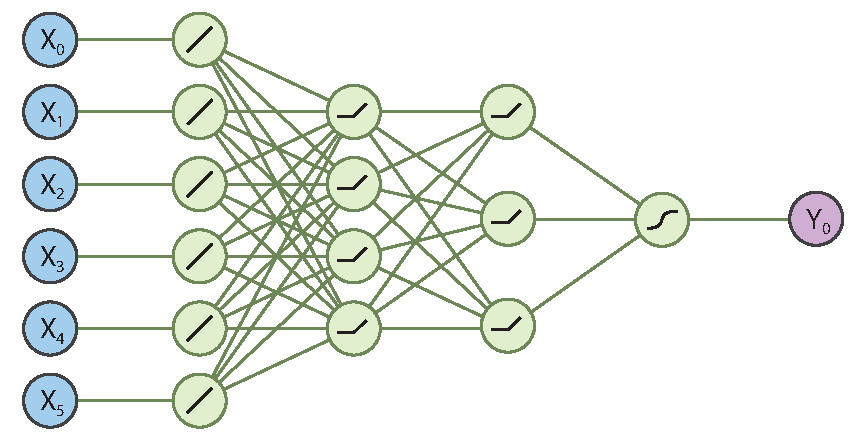
\includegraphics[width=\textwidth]{images/supervised/nn.pdf}
\caption{An example neural network with six inputs, two hidden layers and one output}
\label{fig:nn}
\end{figure}


The basic feed-forward neural network comprises of several building blocks:

\begin{itemize}
\item \textbf{Layer:} Set of neurons in the same depth in the model. The common NN setup includes an input layer (the size of the input), output layer (the size of the output) and one or more hidden layers.

\item \textbf{Activation function:} In each neuron the information propagates through an activation function. The function is often non-linear and it is this function that introduces non-linearity to the whole function approximation process.

The function should meet a few requirements, most importantly it must be continuous and differentiable (If the learning is done using the function's gradient. This is not necessary in other settings, for example evolutionary learning).

Some examples of commonly used activation functions are: (fig \ref{plot:activations})
\begin{figure}[htbp]
%% Creator: Matplotlib, PGF backend
%%
%% To include the figure in your LaTeX document, write
%%   \input{<filename>.pgf}
%%
%% Make sure the required packages are loaded in your preamble
%%   \usepackage{pgf}
%%
%% Figures using additional raster images can only be included by \input if
%% they are in the same directory as the main LaTeX file. For loading figures
%% from other directories you can use the `import` package
%%   \usepackage{import}
%% and then include the figures with
%%   \import{<path to file>}{<filename>.pgf}
%%
%% Matplotlib used the following preamble
%%   \usepackage[utf8x]{inputenc}
%%   \usepackage[T1]{fontenc}
%%
\begingroup%
\makeatletter%
\begin{pgfpicture}%
\pgfpathrectangle{\pgfpointorigin}{\pgfqpoint{5.022831in}{2.009132in}}%
\pgfusepath{use as bounding box, clip}%
\begin{pgfscope}%
\pgfsetbuttcap%
\pgfsetmiterjoin%
\definecolor{currentfill}{rgb}{1.000000,1.000000,1.000000}%
\pgfsetfillcolor{currentfill}%
\pgfsetlinewidth{0.000000pt}%
\definecolor{currentstroke}{rgb}{1.000000,1.000000,1.000000}%
\pgfsetstrokecolor{currentstroke}%
\pgfsetdash{}{0pt}%
\pgfpathmoveto{\pgfqpoint{0.000000in}{0.000000in}}%
\pgfpathlineto{\pgfqpoint{5.022831in}{0.000000in}}%
\pgfpathlineto{\pgfqpoint{5.022831in}{2.009132in}}%
\pgfpathlineto{\pgfqpoint{0.000000in}{2.009132in}}%
\pgfpathclose%
\pgfusepath{fill}%
\end{pgfscope}%
\begin{pgfscope}%
\pgfsetbuttcap%
\pgfsetmiterjoin%
\definecolor{currentfill}{rgb}{1.000000,1.000000,1.000000}%
\pgfsetfillcolor{currentfill}%
\pgfsetlinewidth{0.000000pt}%
\definecolor{currentstroke}{rgb}{0.000000,0.000000,0.000000}%
\pgfsetstrokecolor{currentstroke}%
\pgfsetstrokeopacity{0.000000}%
\pgfsetdash{}{0pt}%
\pgfpathmoveto{\pgfqpoint{0.448229in}{0.303680in}}%
\pgfpathlineto{\pgfqpoint{1.743298in}{0.303680in}}%
\pgfpathlineto{\pgfqpoint{1.743298in}{1.859132in}}%
\pgfpathlineto{\pgfqpoint{0.448229in}{1.859132in}}%
\pgfpathclose%
\pgfusepath{fill}%
\end{pgfscope}%
\begin{pgfscope}%
\pgfpathrectangle{\pgfqpoint{0.448229in}{0.303680in}}{\pgfqpoint{1.295069in}{1.555453in}} %
\pgfusepath{clip}%
\pgfsetrectcap%
\pgfsetroundjoin%
\pgfsetlinewidth{0.501875pt}%
\definecolor{currentstroke}{rgb}{0.000000,0.000000,1.000000}%
\pgfsetstrokecolor{currentstroke}%
\pgfsetdash{}{0pt}%
\pgfpathmoveto{\pgfqpoint{0.448229in}{1.112143in}}%
\pgfpathlineto{\pgfqpoint{0.461310in}{1.113967in}}%
\pgfpathlineto{\pgfqpoint{0.474392in}{1.115893in}}%
\pgfpathlineto{\pgfqpoint{0.487473in}{1.117927in}}%
\pgfpathlineto{\pgfqpoint{0.500555in}{1.120072in}}%
\pgfpathlineto{\pgfqpoint{0.513636in}{1.122336in}}%
\pgfpathlineto{\pgfqpoint{0.526718in}{1.124722in}}%
\pgfpathlineto{\pgfqpoint{0.539799in}{1.127237in}}%
\pgfpathlineto{\pgfqpoint{0.552881in}{1.129886in}}%
\pgfpathlineto{\pgfqpoint{0.565962in}{1.132676in}}%
\pgfpathlineto{\pgfqpoint{0.579044in}{1.135611in}}%
\pgfpathlineto{\pgfqpoint{0.592125in}{1.138698in}}%
\pgfpathlineto{\pgfqpoint{0.605207in}{1.141944in}}%
\pgfpathlineto{\pgfqpoint{0.618288in}{1.145353in}}%
\pgfpathlineto{\pgfqpoint{0.631370in}{1.148932in}}%
\pgfpathlineto{\pgfqpoint{0.644451in}{1.152687in}}%
\pgfpathlineto{\pgfqpoint{0.657533in}{1.156624in}}%
\pgfpathlineto{\pgfqpoint{0.670614in}{1.160748in}}%
\pgfpathlineto{\pgfqpoint{0.683696in}{1.165066in}}%
\pgfpathlineto{\pgfqpoint{0.696777in}{1.169581in}}%
\pgfpathlineto{\pgfqpoint{0.709859in}{1.174301in}}%
\pgfpathlineto{\pgfqpoint{0.722940in}{1.179229in}}%
\pgfpathlineto{\pgfqpoint{0.736022in}{1.184370in}}%
\pgfpathlineto{\pgfqpoint{0.749103in}{1.189728in}}%
\pgfpathlineto{\pgfqpoint{0.762185in}{1.195307in}}%
\pgfpathlineto{\pgfqpoint{0.775266in}{1.201109in}}%
\pgfpathlineto{\pgfqpoint{0.788348in}{1.207137in}}%
\pgfpathlineto{\pgfqpoint{0.801430in}{1.213393in}}%
\pgfpathlineto{\pgfqpoint{0.814511in}{1.219877in}}%
\pgfpathlineto{\pgfqpoint{0.827593in}{1.226591in}}%
\pgfpathlineto{\pgfqpoint{0.840674in}{1.233533in}}%
\pgfpathlineto{\pgfqpoint{0.853756in}{1.240702in}}%
\pgfpathlineto{\pgfqpoint{0.866837in}{1.248095in}}%
\pgfpathlineto{\pgfqpoint{0.879919in}{1.255708in}}%
\pgfpathlineto{\pgfqpoint{0.893000in}{1.263538in}}%
\pgfpathlineto{\pgfqpoint{0.906082in}{1.271579in}}%
\pgfpathlineto{\pgfqpoint{0.919163in}{1.279823in}}%
\pgfpathlineto{\pgfqpoint{0.932245in}{1.288264in}}%
\pgfpathlineto{\pgfqpoint{0.945326in}{1.296891in}}%
\pgfpathlineto{\pgfqpoint{0.958408in}{1.305695in}}%
\pgfpathlineto{\pgfqpoint{0.971489in}{1.314665in}}%
\pgfpathlineto{\pgfqpoint{0.984571in}{1.323789in}}%
\pgfpathlineto{\pgfqpoint{0.997652in}{1.333053in}}%
\pgfpathlineto{\pgfqpoint{1.010734in}{1.342443in}}%
\pgfpathlineto{\pgfqpoint{1.023815in}{1.351945in}}%
\pgfpathlineto{\pgfqpoint{1.036897in}{1.361542in}}%
\pgfpathlineto{\pgfqpoint{1.049978in}{1.371218in}}%
\pgfpathlineto{\pgfqpoint{1.063060in}{1.380956in}}%
\pgfpathlineto{\pgfqpoint{1.076141in}{1.390739in}}%
\pgfpathlineto{\pgfqpoint{1.089223in}{1.400549in}}%
\pgfpathlineto{\pgfqpoint{1.102304in}{1.410368in}}%
\pgfpathlineto{\pgfqpoint{1.115386in}{1.420178in}}%
\pgfpathlineto{\pgfqpoint{1.128467in}{1.429961in}}%
\pgfpathlineto{\pgfqpoint{1.141549in}{1.439700in}}%
\pgfpathlineto{\pgfqpoint{1.154630in}{1.449376in}}%
\pgfpathlineto{\pgfqpoint{1.167712in}{1.458973in}}%
\pgfpathlineto{\pgfqpoint{1.180793in}{1.468474in}}%
\pgfpathlineto{\pgfqpoint{1.193875in}{1.477865in}}%
\pgfpathlineto{\pgfqpoint{1.206956in}{1.487129in}}%
\pgfpathlineto{\pgfqpoint{1.220038in}{1.496252in}}%
\pgfpathlineto{\pgfqpoint{1.233119in}{1.505222in}}%
\pgfpathlineto{\pgfqpoint{1.246201in}{1.514026in}}%
\pgfpathlineto{\pgfqpoint{1.259282in}{1.522654in}}%
\pgfpathlineto{\pgfqpoint{1.272364in}{1.531094in}}%
\pgfpathlineto{\pgfqpoint{1.285445in}{1.539338in}}%
\pgfpathlineto{\pgfqpoint{1.298527in}{1.547379in}}%
\pgfpathlineto{\pgfqpoint{1.311608in}{1.555209in}}%
\pgfpathlineto{\pgfqpoint{1.324690in}{1.562823in}}%
\pgfpathlineto{\pgfqpoint{1.337771in}{1.570216in}}%
\pgfpathlineto{\pgfqpoint{1.350853in}{1.577385in}}%
\pgfpathlineto{\pgfqpoint{1.363934in}{1.584327in}}%
\pgfpathlineto{\pgfqpoint{1.377016in}{1.591040in}}%
\pgfpathlineto{\pgfqpoint{1.390097in}{1.597525in}}%
\pgfpathlineto{\pgfqpoint{1.403179in}{1.603781in}}%
\pgfpathlineto{\pgfqpoint{1.416260in}{1.609809in}}%
\pgfpathlineto{\pgfqpoint{1.429342in}{1.615611in}}%
\pgfpathlineto{\pgfqpoint{1.442423in}{1.621189in}}%
\pgfpathlineto{\pgfqpoint{1.455505in}{1.626547in}}%
\pgfpathlineto{\pgfqpoint{1.468587in}{1.631688in}}%
\pgfpathlineto{\pgfqpoint{1.481668in}{1.636617in}}%
\pgfpathlineto{\pgfqpoint{1.494750in}{1.641336in}}%
\pgfpathlineto{\pgfqpoint{1.507831in}{1.645852in}}%
\pgfpathlineto{\pgfqpoint{1.520913in}{1.650169in}}%
\pgfpathlineto{\pgfqpoint{1.533994in}{1.654294in}}%
\pgfpathlineto{\pgfqpoint{1.547076in}{1.658230in}}%
\pgfpathlineto{\pgfqpoint{1.560157in}{1.661985in}}%
\pgfpathlineto{\pgfqpoint{1.573239in}{1.665565in}}%
\pgfpathlineto{\pgfqpoint{1.586320in}{1.668974in}}%
\pgfpathlineto{\pgfqpoint{1.599402in}{1.672219in}}%
\pgfpathlineto{\pgfqpoint{1.612483in}{1.675306in}}%
\pgfpathlineto{\pgfqpoint{1.625565in}{1.678242in}}%
\pgfpathlineto{\pgfqpoint{1.638646in}{1.681031in}}%
\pgfpathlineto{\pgfqpoint{1.651728in}{1.683681in}}%
\pgfpathlineto{\pgfqpoint{1.664809in}{1.686196in}}%
\pgfpathlineto{\pgfqpoint{1.677891in}{1.688582in}}%
\pgfpathlineto{\pgfqpoint{1.690972in}{1.690845in}}%
\pgfpathlineto{\pgfqpoint{1.704054in}{1.692991in}}%
\pgfpathlineto{\pgfqpoint{1.717135in}{1.695024in}}%
\pgfpathlineto{\pgfqpoint{1.730217in}{1.696950in}}%
\pgfpathlineto{\pgfqpoint{1.743298in}{1.698774in}}%
\pgfusepath{stroke}%
\end{pgfscope}%
\begin{pgfscope}%
\pgfsetrectcap%
\pgfsetmiterjoin%
\pgfsetlinewidth{1.003750pt}%
\definecolor{currentstroke}{rgb}{0.000000,0.000000,0.000000}%
\pgfsetstrokecolor{currentstroke}%
\pgfsetdash{}{0pt}%
\pgfpathmoveto{\pgfqpoint{0.448229in}{1.859132in}}%
\pgfpathlineto{\pgfqpoint{1.743298in}{1.859132in}}%
\pgfusepath{stroke}%
\end{pgfscope}%
\begin{pgfscope}%
\pgfsetrectcap%
\pgfsetmiterjoin%
\pgfsetlinewidth{1.003750pt}%
\definecolor{currentstroke}{rgb}{0.000000,0.000000,0.000000}%
\pgfsetstrokecolor{currentstroke}%
\pgfsetdash{}{0pt}%
\pgfpathmoveto{\pgfqpoint{1.743298in}{0.303680in}}%
\pgfpathlineto{\pgfqpoint{1.743298in}{1.859132in}}%
\pgfusepath{stroke}%
\end{pgfscope}%
\begin{pgfscope}%
\pgfsetrectcap%
\pgfsetmiterjoin%
\pgfsetlinewidth{1.003750pt}%
\definecolor{currentstroke}{rgb}{0.000000,0.000000,0.000000}%
\pgfsetstrokecolor{currentstroke}%
\pgfsetdash{}{0pt}%
\pgfpathmoveto{\pgfqpoint{0.448229in}{0.303680in}}%
\pgfpathlineto{\pgfqpoint{1.743298in}{0.303680in}}%
\pgfusepath{stroke}%
\end{pgfscope}%
\begin{pgfscope}%
\pgfsetrectcap%
\pgfsetmiterjoin%
\pgfsetlinewidth{1.003750pt}%
\definecolor{currentstroke}{rgb}{0.000000,0.000000,0.000000}%
\pgfsetstrokecolor{currentstroke}%
\pgfsetdash{}{0pt}%
\pgfpathmoveto{\pgfqpoint{0.448229in}{0.303680in}}%
\pgfpathlineto{\pgfqpoint{0.448229in}{1.859132in}}%
\pgfusepath{stroke}%
\end{pgfscope}%
\begin{pgfscope}%
\pgfpathrectangle{\pgfqpoint{0.448229in}{0.303680in}}{\pgfqpoint{1.295069in}{1.555453in}} %
\pgfusepath{clip}%
\pgfsetbuttcap%
\pgfsetroundjoin%
\pgfsetlinewidth{0.501875pt}%
\definecolor{currentstroke}{rgb}{0.000000,0.000000,0.000000}%
\pgfsetstrokecolor{currentstroke}%
\pgfsetdash{{1.000000pt}{3.000000pt}}{0.000000pt}%
\pgfpathmoveto{\pgfqpoint{0.448229in}{0.303680in}}%
\pgfpathlineto{\pgfqpoint{0.448229in}{1.859132in}}%
\pgfusepath{stroke}%
\end{pgfscope}%
\begin{pgfscope}%
\pgfsetbuttcap%
\pgfsetroundjoin%
\definecolor{currentfill}{rgb}{0.000000,0.000000,0.000000}%
\pgfsetfillcolor{currentfill}%
\pgfsetlinewidth{0.501875pt}%
\definecolor{currentstroke}{rgb}{0.000000,0.000000,0.000000}%
\pgfsetstrokecolor{currentstroke}%
\pgfsetdash{}{0pt}%
\pgfsys@defobject{currentmarker}{\pgfqpoint{0.000000in}{0.000000in}}{\pgfqpoint{0.000000in}{0.055556in}}{%
\pgfpathmoveto{\pgfqpoint{0.000000in}{0.000000in}}%
\pgfpathlineto{\pgfqpoint{0.000000in}{0.055556in}}%
\pgfusepath{stroke,fill}%
}%
\begin{pgfscope}%
\pgfsys@transformshift{0.448229in}{0.303680in}%
\pgfsys@useobject{currentmarker}{}%
\end{pgfscope}%
\end{pgfscope}%
\begin{pgfscope}%
\pgfsetbuttcap%
\pgfsetroundjoin%
\definecolor{currentfill}{rgb}{0.000000,0.000000,0.000000}%
\pgfsetfillcolor{currentfill}%
\pgfsetlinewidth{0.501875pt}%
\definecolor{currentstroke}{rgb}{0.000000,0.000000,0.000000}%
\pgfsetstrokecolor{currentstroke}%
\pgfsetdash{}{0pt}%
\pgfsys@defobject{currentmarker}{\pgfqpoint{0.000000in}{-0.055556in}}{\pgfqpoint{0.000000in}{0.000000in}}{%
\pgfpathmoveto{\pgfqpoint{0.000000in}{0.000000in}}%
\pgfpathlineto{\pgfqpoint{0.000000in}{-0.055556in}}%
\pgfusepath{stroke,fill}%
}%
\begin{pgfscope}%
\pgfsys@transformshift{0.448229in}{1.859132in}%
\pgfsys@useobject{currentmarker}{}%
\end{pgfscope}%
\end{pgfscope}%
\begin{pgfscope}%
\pgftext[x=0.448229in,y=0.248124in,,top]{\fontsize{8.000000}{9.600000}\selectfont \(\displaystyle -3\)}%
\end{pgfscope}%
\begin{pgfscope}%
\pgfpathrectangle{\pgfqpoint{0.448229in}{0.303680in}}{\pgfqpoint{1.295069in}{1.555453in}} %
\pgfusepath{clip}%
\pgfsetbuttcap%
\pgfsetroundjoin%
\pgfsetlinewidth{0.501875pt}%
\definecolor{currentstroke}{rgb}{0.000000,0.000000,0.000000}%
\pgfsetstrokecolor{currentstroke}%
\pgfsetdash{{1.000000pt}{3.000000pt}}{0.000000pt}%
\pgfpathmoveto{\pgfqpoint{0.664074in}{0.303680in}}%
\pgfpathlineto{\pgfqpoint{0.664074in}{1.859132in}}%
\pgfusepath{stroke}%
\end{pgfscope}%
\begin{pgfscope}%
\pgfsetbuttcap%
\pgfsetroundjoin%
\definecolor{currentfill}{rgb}{0.000000,0.000000,0.000000}%
\pgfsetfillcolor{currentfill}%
\pgfsetlinewidth{0.501875pt}%
\definecolor{currentstroke}{rgb}{0.000000,0.000000,0.000000}%
\pgfsetstrokecolor{currentstroke}%
\pgfsetdash{}{0pt}%
\pgfsys@defobject{currentmarker}{\pgfqpoint{0.000000in}{0.000000in}}{\pgfqpoint{0.000000in}{0.055556in}}{%
\pgfpathmoveto{\pgfqpoint{0.000000in}{0.000000in}}%
\pgfpathlineto{\pgfqpoint{0.000000in}{0.055556in}}%
\pgfusepath{stroke,fill}%
}%
\begin{pgfscope}%
\pgfsys@transformshift{0.664074in}{0.303680in}%
\pgfsys@useobject{currentmarker}{}%
\end{pgfscope}%
\end{pgfscope}%
\begin{pgfscope}%
\pgfsetbuttcap%
\pgfsetroundjoin%
\definecolor{currentfill}{rgb}{0.000000,0.000000,0.000000}%
\pgfsetfillcolor{currentfill}%
\pgfsetlinewidth{0.501875pt}%
\definecolor{currentstroke}{rgb}{0.000000,0.000000,0.000000}%
\pgfsetstrokecolor{currentstroke}%
\pgfsetdash{}{0pt}%
\pgfsys@defobject{currentmarker}{\pgfqpoint{0.000000in}{-0.055556in}}{\pgfqpoint{0.000000in}{0.000000in}}{%
\pgfpathmoveto{\pgfqpoint{0.000000in}{0.000000in}}%
\pgfpathlineto{\pgfqpoint{0.000000in}{-0.055556in}}%
\pgfusepath{stroke,fill}%
}%
\begin{pgfscope}%
\pgfsys@transformshift{0.664074in}{1.859132in}%
\pgfsys@useobject{currentmarker}{}%
\end{pgfscope}%
\end{pgfscope}%
\begin{pgfscope}%
\pgftext[x=0.664074in,y=0.248124in,,top]{\fontsize{8.000000}{9.600000}\selectfont \(\displaystyle -2\)}%
\end{pgfscope}%
\begin{pgfscope}%
\pgfpathrectangle{\pgfqpoint{0.448229in}{0.303680in}}{\pgfqpoint{1.295069in}{1.555453in}} %
\pgfusepath{clip}%
\pgfsetbuttcap%
\pgfsetroundjoin%
\pgfsetlinewidth{0.501875pt}%
\definecolor{currentstroke}{rgb}{0.000000,0.000000,0.000000}%
\pgfsetstrokecolor{currentstroke}%
\pgfsetdash{{1.000000pt}{3.000000pt}}{0.000000pt}%
\pgfpathmoveto{\pgfqpoint{0.879919in}{0.303680in}}%
\pgfpathlineto{\pgfqpoint{0.879919in}{1.859132in}}%
\pgfusepath{stroke}%
\end{pgfscope}%
\begin{pgfscope}%
\pgfsetbuttcap%
\pgfsetroundjoin%
\definecolor{currentfill}{rgb}{0.000000,0.000000,0.000000}%
\pgfsetfillcolor{currentfill}%
\pgfsetlinewidth{0.501875pt}%
\definecolor{currentstroke}{rgb}{0.000000,0.000000,0.000000}%
\pgfsetstrokecolor{currentstroke}%
\pgfsetdash{}{0pt}%
\pgfsys@defobject{currentmarker}{\pgfqpoint{0.000000in}{0.000000in}}{\pgfqpoint{0.000000in}{0.055556in}}{%
\pgfpathmoveto{\pgfqpoint{0.000000in}{0.000000in}}%
\pgfpathlineto{\pgfqpoint{0.000000in}{0.055556in}}%
\pgfusepath{stroke,fill}%
}%
\begin{pgfscope}%
\pgfsys@transformshift{0.879919in}{0.303680in}%
\pgfsys@useobject{currentmarker}{}%
\end{pgfscope}%
\end{pgfscope}%
\begin{pgfscope}%
\pgfsetbuttcap%
\pgfsetroundjoin%
\definecolor{currentfill}{rgb}{0.000000,0.000000,0.000000}%
\pgfsetfillcolor{currentfill}%
\pgfsetlinewidth{0.501875pt}%
\definecolor{currentstroke}{rgb}{0.000000,0.000000,0.000000}%
\pgfsetstrokecolor{currentstroke}%
\pgfsetdash{}{0pt}%
\pgfsys@defobject{currentmarker}{\pgfqpoint{0.000000in}{-0.055556in}}{\pgfqpoint{0.000000in}{0.000000in}}{%
\pgfpathmoveto{\pgfqpoint{0.000000in}{0.000000in}}%
\pgfpathlineto{\pgfqpoint{0.000000in}{-0.055556in}}%
\pgfusepath{stroke,fill}%
}%
\begin{pgfscope}%
\pgfsys@transformshift{0.879919in}{1.859132in}%
\pgfsys@useobject{currentmarker}{}%
\end{pgfscope}%
\end{pgfscope}%
\begin{pgfscope}%
\pgftext[x=0.879919in,y=0.248124in,,top]{\fontsize{8.000000}{9.600000}\selectfont \(\displaystyle -1\)}%
\end{pgfscope}%
\begin{pgfscope}%
\pgfpathrectangle{\pgfqpoint{0.448229in}{0.303680in}}{\pgfqpoint{1.295069in}{1.555453in}} %
\pgfusepath{clip}%
\pgfsetbuttcap%
\pgfsetroundjoin%
\pgfsetlinewidth{0.501875pt}%
\definecolor{currentstroke}{rgb}{0.000000,0.000000,0.000000}%
\pgfsetstrokecolor{currentstroke}%
\pgfsetdash{{1.000000pt}{3.000000pt}}{0.000000pt}%
\pgfpathmoveto{\pgfqpoint{1.095763in}{0.303680in}}%
\pgfpathlineto{\pgfqpoint{1.095763in}{1.859132in}}%
\pgfusepath{stroke}%
\end{pgfscope}%
\begin{pgfscope}%
\pgfsetbuttcap%
\pgfsetroundjoin%
\definecolor{currentfill}{rgb}{0.000000,0.000000,0.000000}%
\pgfsetfillcolor{currentfill}%
\pgfsetlinewidth{0.501875pt}%
\definecolor{currentstroke}{rgb}{0.000000,0.000000,0.000000}%
\pgfsetstrokecolor{currentstroke}%
\pgfsetdash{}{0pt}%
\pgfsys@defobject{currentmarker}{\pgfqpoint{0.000000in}{0.000000in}}{\pgfqpoint{0.000000in}{0.055556in}}{%
\pgfpathmoveto{\pgfqpoint{0.000000in}{0.000000in}}%
\pgfpathlineto{\pgfqpoint{0.000000in}{0.055556in}}%
\pgfusepath{stroke,fill}%
}%
\begin{pgfscope}%
\pgfsys@transformshift{1.095763in}{0.303680in}%
\pgfsys@useobject{currentmarker}{}%
\end{pgfscope}%
\end{pgfscope}%
\begin{pgfscope}%
\pgfsetbuttcap%
\pgfsetroundjoin%
\definecolor{currentfill}{rgb}{0.000000,0.000000,0.000000}%
\pgfsetfillcolor{currentfill}%
\pgfsetlinewidth{0.501875pt}%
\definecolor{currentstroke}{rgb}{0.000000,0.000000,0.000000}%
\pgfsetstrokecolor{currentstroke}%
\pgfsetdash{}{0pt}%
\pgfsys@defobject{currentmarker}{\pgfqpoint{0.000000in}{-0.055556in}}{\pgfqpoint{0.000000in}{0.000000in}}{%
\pgfpathmoveto{\pgfqpoint{0.000000in}{0.000000in}}%
\pgfpathlineto{\pgfqpoint{0.000000in}{-0.055556in}}%
\pgfusepath{stroke,fill}%
}%
\begin{pgfscope}%
\pgfsys@transformshift{1.095763in}{1.859132in}%
\pgfsys@useobject{currentmarker}{}%
\end{pgfscope}%
\end{pgfscope}%
\begin{pgfscope}%
\pgftext[x=1.095763in,y=0.248124in,,top]{\fontsize{8.000000}{9.600000}\selectfont \(\displaystyle 0\)}%
\end{pgfscope}%
\begin{pgfscope}%
\pgfpathrectangle{\pgfqpoint{0.448229in}{0.303680in}}{\pgfqpoint{1.295069in}{1.555453in}} %
\pgfusepath{clip}%
\pgfsetbuttcap%
\pgfsetroundjoin%
\pgfsetlinewidth{0.501875pt}%
\definecolor{currentstroke}{rgb}{0.000000,0.000000,0.000000}%
\pgfsetstrokecolor{currentstroke}%
\pgfsetdash{{1.000000pt}{3.000000pt}}{0.000000pt}%
\pgfpathmoveto{\pgfqpoint{1.311608in}{0.303680in}}%
\pgfpathlineto{\pgfqpoint{1.311608in}{1.859132in}}%
\pgfusepath{stroke}%
\end{pgfscope}%
\begin{pgfscope}%
\pgfsetbuttcap%
\pgfsetroundjoin%
\definecolor{currentfill}{rgb}{0.000000,0.000000,0.000000}%
\pgfsetfillcolor{currentfill}%
\pgfsetlinewidth{0.501875pt}%
\definecolor{currentstroke}{rgb}{0.000000,0.000000,0.000000}%
\pgfsetstrokecolor{currentstroke}%
\pgfsetdash{}{0pt}%
\pgfsys@defobject{currentmarker}{\pgfqpoint{0.000000in}{0.000000in}}{\pgfqpoint{0.000000in}{0.055556in}}{%
\pgfpathmoveto{\pgfqpoint{0.000000in}{0.000000in}}%
\pgfpathlineto{\pgfqpoint{0.000000in}{0.055556in}}%
\pgfusepath{stroke,fill}%
}%
\begin{pgfscope}%
\pgfsys@transformshift{1.311608in}{0.303680in}%
\pgfsys@useobject{currentmarker}{}%
\end{pgfscope}%
\end{pgfscope}%
\begin{pgfscope}%
\pgfsetbuttcap%
\pgfsetroundjoin%
\definecolor{currentfill}{rgb}{0.000000,0.000000,0.000000}%
\pgfsetfillcolor{currentfill}%
\pgfsetlinewidth{0.501875pt}%
\definecolor{currentstroke}{rgb}{0.000000,0.000000,0.000000}%
\pgfsetstrokecolor{currentstroke}%
\pgfsetdash{}{0pt}%
\pgfsys@defobject{currentmarker}{\pgfqpoint{0.000000in}{-0.055556in}}{\pgfqpoint{0.000000in}{0.000000in}}{%
\pgfpathmoveto{\pgfqpoint{0.000000in}{0.000000in}}%
\pgfpathlineto{\pgfqpoint{0.000000in}{-0.055556in}}%
\pgfusepath{stroke,fill}%
}%
\begin{pgfscope}%
\pgfsys@transformshift{1.311608in}{1.859132in}%
\pgfsys@useobject{currentmarker}{}%
\end{pgfscope}%
\end{pgfscope}%
\begin{pgfscope}%
\pgftext[x=1.311608in,y=0.248124in,,top]{\fontsize{8.000000}{9.600000}\selectfont \(\displaystyle 1\)}%
\end{pgfscope}%
\begin{pgfscope}%
\pgfpathrectangle{\pgfqpoint{0.448229in}{0.303680in}}{\pgfqpoint{1.295069in}{1.555453in}} %
\pgfusepath{clip}%
\pgfsetbuttcap%
\pgfsetroundjoin%
\pgfsetlinewidth{0.501875pt}%
\definecolor{currentstroke}{rgb}{0.000000,0.000000,0.000000}%
\pgfsetstrokecolor{currentstroke}%
\pgfsetdash{{1.000000pt}{3.000000pt}}{0.000000pt}%
\pgfpathmoveto{\pgfqpoint{1.527453in}{0.303680in}}%
\pgfpathlineto{\pgfqpoint{1.527453in}{1.859132in}}%
\pgfusepath{stroke}%
\end{pgfscope}%
\begin{pgfscope}%
\pgfsetbuttcap%
\pgfsetroundjoin%
\definecolor{currentfill}{rgb}{0.000000,0.000000,0.000000}%
\pgfsetfillcolor{currentfill}%
\pgfsetlinewidth{0.501875pt}%
\definecolor{currentstroke}{rgb}{0.000000,0.000000,0.000000}%
\pgfsetstrokecolor{currentstroke}%
\pgfsetdash{}{0pt}%
\pgfsys@defobject{currentmarker}{\pgfqpoint{0.000000in}{0.000000in}}{\pgfqpoint{0.000000in}{0.055556in}}{%
\pgfpathmoveto{\pgfqpoint{0.000000in}{0.000000in}}%
\pgfpathlineto{\pgfqpoint{0.000000in}{0.055556in}}%
\pgfusepath{stroke,fill}%
}%
\begin{pgfscope}%
\pgfsys@transformshift{1.527453in}{0.303680in}%
\pgfsys@useobject{currentmarker}{}%
\end{pgfscope}%
\end{pgfscope}%
\begin{pgfscope}%
\pgfsetbuttcap%
\pgfsetroundjoin%
\definecolor{currentfill}{rgb}{0.000000,0.000000,0.000000}%
\pgfsetfillcolor{currentfill}%
\pgfsetlinewidth{0.501875pt}%
\definecolor{currentstroke}{rgb}{0.000000,0.000000,0.000000}%
\pgfsetstrokecolor{currentstroke}%
\pgfsetdash{}{0pt}%
\pgfsys@defobject{currentmarker}{\pgfqpoint{0.000000in}{-0.055556in}}{\pgfqpoint{0.000000in}{0.000000in}}{%
\pgfpathmoveto{\pgfqpoint{0.000000in}{0.000000in}}%
\pgfpathlineto{\pgfqpoint{0.000000in}{-0.055556in}}%
\pgfusepath{stroke,fill}%
}%
\begin{pgfscope}%
\pgfsys@transformshift{1.527453in}{1.859132in}%
\pgfsys@useobject{currentmarker}{}%
\end{pgfscope}%
\end{pgfscope}%
\begin{pgfscope}%
\pgftext[x=1.527453in,y=0.248124in,,top]{\fontsize{8.000000}{9.600000}\selectfont \(\displaystyle 2\)}%
\end{pgfscope}%
\begin{pgfscope}%
\pgfpathrectangle{\pgfqpoint{0.448229in}{0.303680in}}{\pgfqpoint{1.295069in}{1.555453in}} %
\pgfusepath{clip}%
\pgfsetbuttcap%
\pgfsetroundjoin%
\pgfsetlinewidth{0.501875pt}%
\definecolor{currentstroke}{rgb}{0.000000,0.000000,0.000000}%
\pgfsetstrokecolor{currentstroke}%
\pgfsetdash{{1.000000pt}{3.000000pt}}{0.000000pt}%
\pgfpathmoveto{\pgfqpoint{1.743298in}{0.303680in}}%
\pgfpathlineto{\pgfqpoint{1.743298in}{1.859132in}}%
\pgfusepath{stroke}%
\end{pgfscope}%
\begin{pgfscope}%
\pgfsetbuttcap%
\pgfsetroundjoin%
\definecolor{currentfill}{rgb}{0.000000,0.000000,0.000000}%
\pgfsetfillcolor{currentfill}%
\pgfsetlinewidth{0.501875pt}%
\definecolor{currentstroke}{rgb}{0.000000,0.000000,0.000000}%
\pgfsetstrokecolor{currentstroke}%
\pgfsetdash{}{0pt}%
\pgfsys@defobject{currentmarker}{\pgfqpoint{0.000000in}{0.000000in}}{\pgfqpoint{0.000000in}{0.055556in}}{%
\pgfpathmoveto{\pgfqpoint{0.000000in}{0.000000in}}%
\pgfpathlineto{\pgfqpoint{0.000000in}{0.055556in}}%
\pgfusepath{stroke,fill}%
}%
\begin{pgfscope}%
\pgfsys@transformshift{1.743298in}{0.303680in}%
\pgfsys@useobject{currentmarker}{}%
\end{pgfscope}%
\end{pgfscope}%
\begin{pgfscope}%
\pgfsetbuttcap%
\pgfsetroundjoin%
\definecolor{currentfill}{rgb}{0.000000,0.000000,0.000000}%
\pgfsetfillcolor{currentfill}%
\pgfsetlinewidth{0.501875pt}%
\definecolor{currentstroke}{rgb}{0.000000,0.000000,0.000000}%
\pgfsetstrokecolor{currentstroke}%
\pgfsetdash{}{0pt}%
\pgfsys@defobject{currentmarker}{\pgfqpoint{0.000000in}{-0.055556in}}{\pgfqpoint{0.000000in}{0.000000in}}{%
\pgfpathmoveto{\pgfqpoint{0.000000in}{0.000000in}}%
\pgfpathlineto{\pgfqpoint{0.000000in}{-0.055556in}}%
\pgfusepath{stroke,fill}%
}%
\begin{pgfscope}%
\pgfsys@transformshift{1.743298in}{1.859132in}%
\pgfsys@useobject{currentmarker}{}%
\end{pgfscope}%
\end{pgfscope}%
\begin{pgfscope}%
\pgftext[x=1.743298in,y=0.248124in,,top]{\fontsize{8.000000}{9.600000}\selectfont \(\displaystyle 3\)}%
\end{pgfscope}%
\begin{pgfscope}%
\pgfpathrectangle{\pgfqpoint{0.448229in}{0.303680in}}{\pgfqpoint{1.295069in}{1.555453in}} %
\pgfusepath{clip}%
\pgfsetbuttcap%
\pgfsetroundjoin%
\pgfsetlinewidth{0.501875pt}%
\definecolor{currentstroke}{rgb}{0.000000,0.000000,0.000000}%
\pgfsetstrokecolor{currentstroke}%
\pgfsetdash{{1.000000pt}{3.000000pt}}{0.000000pt}%
\pgfpathmoveto{\pgfqpoint{0.448229in}{0.433301in}}%
\pgfpathlineto{\pgfqpoint{1.743298in}{0.433301in}}%
\pgfusepath{stroke}%
\end{pgfscope}%
\begin{pgfscope}%
\pgfsetbuttcap%
\pgfsetroundjoin%
\definecolor{currentfill}{rgb}{0.000000,0.000000,0.000000}%
\pgfsetfillcolor{currentfill}%
\pgfsetlinewidth{0.501875pt}%
\definecolor{currentstroke}{rgb}{0.000000,0.000000,0.000000}%
\pgfsetstrokecolor{currentstroke}%
\pgfsetdash{}{0pt}%
\pgfsys@defobject{currentmarker}{\pgfqpoint{0.000000in}{0.000000in}}{\pgfqpoint{0.055556in}{0.000000in}}{%
\pgfpathmoveto{\pgfqpoint{0.000000in}{0.000000in}}%
\pgfpathlineto{\pgfqpoint{0.055556in}{0.000000in}}%
\pgfusepath{stroke,fill}%
}%
\begin{pgfscope}%
\pgfsys@transformshift{0.448229in}{0.433301in}%
\pgfsys@useobject{currentmarker}{}%
\end{pgfscope}%
\end{pgfscope}%
\begin{pgfscope}%
\pgfsetbuttcap%
\pgfsetroundjoin%
\definecolor{currentfill}{rgb}{0.000000,0.000000,0.000000}%
\pgfsetfillcolor{currentfill}%
\pgfsetlinewidth{0.501875pt}%
\definecolor{currentstroke}{rgb}{0.000000,0.000000,0.000000}%
\pgfsetstrokecolor{currentstroke}%
\pgfsetdash{}{0pt}%
\pgfsys@defobject{currentmarker}{\pgfqpoint{-0.055556in}{0.000000in}}{\pgfqpoint{0.000000in}{0.000000in}}{%
\pgfpathmoveto{\pgfqpoint{0.000000in}{0.000000in}}%
\pgfpathlineto{\pgfqpoint{-0.055556in}{0.000000in}}%
\pgfusepath{stroke,fill}%
}%
\begin{pgfscope}%
\pgfsys@transformshift{1.743298in}{0.433301in}%
\pgfsys@useobject{currentmarker}{}%
\end{pgfscope}%
\end{pgfscope}%
\begin{pgfscope}%
\pgftext[x=0.392673in,y=0.433301in,right,]{\fontsize{8.000000}{9.600000}\selectfont \(\displaystyle -1.0\)}%
\end{pgfscope}%
\begin{pgfscope}%
\pgfpathrectangle{\pgfqpoint{0.448229in}{0.303680in}}{\pgfqpoint{1.295069in}{1.555453in}} %
\pgfusepath{clip}%
\pgfsetbuttcap%
\pgfsetroundjoin%
\pgfsetlinewidth{0.501875pt}%
\definecolor{currentstroke}{rgb}{0.000000,0.000000,0.000000}%
\pgfsetstrokecolor{currentstroke}%
\pgfsetdash{{1.000000pt}{3.000000pt}}{0.000000pt}%
\pgfpathmoveto{\pgfqpoint{0.448229in}{0.757354in}}%
\pgfpathlineto{\pgfqpoint{1.743298in}{0.757354in}}%
\pgfusepath{stroke}%
\end{pgfscope}%
\begin{pgfscope}%
\pgfsetbuttcap%
\pgfsetroundjoin%
\definecolor{currentfill}{rgb}{0.000000,0.000000,0.000000}%
\pgfsetfillcolor{currentfill}%
\pgfsetlinewidth{0.501875pt}%
\definecolor{currentstroke}{rgb}{0.000000,0.000000,0.000000}%
\pgfsetstrokecolor{currentstroke}%
\pgfsetdash{}{0pt}%
\pgfsys@defobject{currentmarker}{\pgfqpoint{0.000000in}{0.000000in}}{\pgfqpoint{0.055556in}{0.000000in}}{%
\pgfpathmoveto{\pgfqpoint{0.000000in}{0.000000in}}%
\pgfpathlineto{\pgfqpoint{0.055556in}{0.000000in}}%
\pgfusepath{stroke,fill}%
}%
\begin{pgfscope}%
\pgfsys@transformshift{0.448229in}{0.757354in}%
\pgfsys@useobject{currentmarker}{}%
\end{pgfscope}%
\end{pgfscope}%
\begin{pgfscope}%
\pgfsetbuttcap%
\pgfsetroundjoin%
\definecolor{currentfill}{rgb}{0.000000,0.000000,0.000000}%
\pgfsetfillcolor{currentfill}%
\pgfsetlinewidth{0.501875pt}%
\definecolor{currentstroke}{rgb}{0.000000,0.000000,0.000000}%
\pgfsetstrokecolor{currentstroke}%
\pgfsetdash{}{0pt}%
\pgfsys@defobject{currentmarker}{\pgfqpoint{-0.055556in}{0.000000in}}{\pgfqpoint{0.000000in}{0.000000in}}{%
\pgfpathmoveto{\pgfqpoint{0.000000in}{0.000000in}}%
\pgfpathlineto{\pgfqpoint{-0.055556in}{0.000000in}}%
\pgfusepath{stroke,fill}%
}%
\begin{pgfscope}%
\pgfsys@transformshift{1.743298in}{0.757354in}%
\pgfsys@useobject{currentmarker}{}%
\end{pgfscope}%
\end{pgfscope}%
\begin{pgfscope}%
\pgftext[x=0.392673in,y=0.757354in,right,]{\fontsize{8.000000}{9.600000}\selectfont \(\displaystyle -0.5\)}%
\end{pgfscope}%
\begin{pgfscope}%
\pgfpathrectangle{\pgfqpoint{0.448229in}{0.303680in}}{\pgfqpoint{1.295069in}{1.555453in}} %
\pgfusepath{clip}%
\pgfsetbuttcap%
\pgfsetroundjoin%
\pgfsetlinewidth{0.501875pt}%
\definecolor{currentstroke}{rgb}{0.000000,0.000000,0.000000}%
\pgfsetstrokecolor{currentstroke}%
\pgfsetdash{{1.000000pt}{3.000000pt}}{0.000000pt}%
\pgfpathmoveto{\pgfqpoint{0.448229in}{1.081406in}}%
\pgfpathlineto{\pgfqpoint{1.743298in}{1.081406in}}%
\pgfusepath{stroke}%
\end{pgfscope}%
\begin{pgfscope}%
\pgfsetbuttcap%
\pgfsetroundjoin%
\definecolor{currentfill}{rgb}{0.000000,0.000000,0.000000}%
\pgfsetfillcolor{currentfill}%
\pgfsetlinewidth{0.501875pt}%
\definecolor{currentstroke}{rgb}{0.000000,0.000000,0.000000}%
\pgfsetstrokecolor{currentstroke}%
\pgfsetdash{}{0pt}%
\pgfsys@defobject{currentmarker}{\pgfqpoint{0.000000in}{0.000000in}}{\pgfqpoint{0.055556in}{0.000000in}}{%
\pgfpathmoveto{\pgfqpoint{0.000000in}{0.000000in}}%
\pgfpathlineto{\pgfqpoint{0.055556in}{0.000000in}}%
\pgfusepath{stroke,fill}%
}%
\begin{pgfscope}%
\pgfsys@transformshift{0.448229in}{1.081406in}%
\pgfsys@useobject{currentmarker}{}%
\end{pgfscope}%
\end{pgfscope}%
\begin{pgfscope}%
\pgfsetbuttcap%
\pgfsetroundjoin%
\definecolor{currentfill}{rgb}{0.000000,0.000000,0.000000}%
\pgfsetfillcolor{currentfill}%
\pgfsetlinewidth{0.501875pt}%
\definecolor{currentstroke}{rgb}{0.000000,0.000000,0.000000}%
\pgfsetstrokecolor{currentstroke}%
\pgfsetdash{}{0pt}%
\pgfsys@defobject{currentmarker}{\pgfqpoint{-0.055556in}{0.000000in}}{\pgfqpoint{0.000000in}{0.000000in}}{%
\pgfpathmoveto{\pgfqpoint{0.000000in}{0.000000in}}%
\pgfpathlineto{\pgfqpoint{-0.055556in}{0.000000in}}%
\pgfusepath{stroke,fill}%
}%
\begin{pgfscope}%
\pgfsys@transformshift{1.743298in}{1.081406in}%
\pgfsys@useobject{currentmarker}{}%
\end{pgfscope}%
\end{pgfscope}%
\begin{pgfscope}%
\pgftext[x=0.392673in,y=1.081406in,right,]{\fontsize{8.000000}{9.600000}\selectfont \(\displaystyle 0.0\)}%
\end{pgfscope}%
\begin{pgfscope}%
\pgfpathrectangle{\pgfqpoint{0.448229in}{0.303680in}}{\pgfqpoint{1.295069in}{1.555453in}} %
\pgfusepath{clip}%
\pgfsetbuttcap%
\pgfsetroundjoin%
\pgfsetlinewidth{0.501875pt}%
\definecolor{currentstroke}{rgb}{0.000000,0.000000,0.000000}%
\pgfsetstrokecolor{currentstroke}%
\pgfsetdash{{1.000000pt}{3.000000pt}}{0.000000pt}%
\pgfpathmoveto{\pgfqpoint{0.448229in}{1.405459in}}%
\pgfpathlineto{\pgfqpoint{1.743298in}{1.405459in}}%
\pgfusepath{stroke}%
\end{pgfscope}%
\begin{pgfscope}%
\pgfsetbuttcap%
\pgfsetroundjoin%
\definecolor{currentfill}{rgb}{0.000000,0.000000,0.000000}%
\pgfsetfillcolor{currentfill}%
\pgfsetlinewidth{0.501875pt}%
\definecolor{currentstroke}{rgb}{0.000000,0.000000,0.000000}%
\pgfsetstrokecolor{currentstroke}%
\pgfsetdash{}{0pt}%
\pgfsys@defobject{currentmarker}{\pgfqpoint{0.000000in}{0.000000in}}{\pgfqpoint{0.055556in}{0.000000in}}{%
\pgfpathmoveto{\pgfqpoint{0.000000in}{0.000000in}}%
\pgfpathlineto{\pgfqpoint{0.055556in}{0.000000in}}%
\pgfusepath{stroke,fill}%
}%
\begin{pgfscope}%
\pgfsys@transformshift{0.448229in}{1.405459in}%
\pgfsys@useobject{currentmarker}{}%
\end{pgfscope}%
\end{pgfscope}%
\begin{pgfscope}%
\pgfsetbuttcap%
\pgfsetroundjoin%
\definecolor{currentfill}{rgb}{0.000000,0.000000,0.000000}%
\pgfsetfillcolor{currentfill}%
\pgfsetlinewidth{0.501875pt}%
\definecolor{currentstroke}{rgb}{0.000000,0.000000,0.000000}%
\pgfsetstrokecolor{currentstroke}%
\pgfsetdash{}{0pt}%
\pgfsys@defobject{currentmarker}{\pgfqpoint{-0.055556in}{0.000000in}}{\pgfqpoint{0.000000in}{0.000000in}}{%
\pgfpathmoveto{\pgfqpoint{0.000000in}{0.000000in}}%
\pgfpathlineto{\pgfqpoint{-0.055556in}{0.000000in}}%
\pgfusepath{stroke,fill}%
}%
\begin{pgfscope}%
\pgfsys@transformshift{1.743298in}{1.405459in}%
\pgfsys@useobject{currentmarker}{}%
\end{pgfscope}%
\end{pgfscope}%
\begin{pgfscope}%
\pgftext[x=0.392673in,y=1.405459in,right,]{\fontsize{8.000000}{9.600000}\selectfont \(\displaystyle 0.5\)}%
\end{pgfscope}%
\begin{pgfscope}%
\pgfpathrectangle{\pgfqpoint{0.448229in}{0.303680in}}{\pgfqpoint{1.295069in}{1.555453in}} %
\pgfusepath{clip}%
\pgfsetbuttcap%
\pgfsetroundjoin%
\pgfsetlinewidth{0.501875pt}%
\definecolor{currentstroke}{rgb}{0.000000,0.000000,0.000000}%
\pgfsetstrokecolor{currentstroke}%
\pgfsetdash{{1.000000pt}{3.000000pt}}{0.000000pt}%
\pgfpathmoveto{\pgfqpoint{0.448229in}{1.729511in}}%
\pgfpathlineto{\pgfqpoint{1.743298in}{1.729511in}}%
\pgfusepath{stroke}%
\end{pgfscope}%
\begin{pgfscope}%
\pgfsetbuttcap%
\pgfsetroundjoin%
\definecolor{currentfill}{rgb}{0.000000,0.000000,0.000000}%
\pgfsetfillcolor{currentfill}%
\pgfsetlinewidth{0.501875pt}%
\definecolor{currentstroke}{rgb}{0.000000,0.000000,0.000000}%
\pgfsetstrokecolor{currentstroke}%
\pgfsetdash{}{0pt}%
\pgfsys@defobject{currentmarker}{\pgfqpoint{0.000000in}{0.000000in}}{\pgfqpoint{0.055556in}{0.000000in}}{%
\pgfpathmoveto{\pgfqpoint{0.000000in}{0.000000in}}%
\pgfpathlineto{\pgfqpoint{0.055556in}{0.000000in}}%
\pgfusepath{stroke,fill}%
}%
\begin{pgfscope}%
\pgfsys@transformshift{0.448229in}{1.729511in}%
\pgfsys@useobject{currentmarker}{}%
\end{pgfscope}%
\end{pgfscope}%
\begin{pgfscope}%
\pgfsetbuttcap%
\pgfsetroundjoin%
\definecolor{currentfill}{rgb}{0.000000,0.000000,0.000000}%
\pgfsetfillcolor{currentfill}%
\pgfsetlinewidth{0.501875pt}%
\definecolor{currentstroke}{rgb}{0.000000,0.000000,0.000000}%
\pgfsetstrokecolor{currentstroke}%
\pgfsetdash{}{0pt}%
\pgfsys@defobject{currentmarker}{\pgfqpoint{-0.055556in}{0.000000in}}{\pgfqpoint{0.000000in}{0.000000in}}{%
\pgfpathmoveto{\pgfqpoint{0.000000in}{0.000000in}}%
\pgfpathlineto{\pgfqpoint{-0.055556in}{0.000000in}}%
\pgfusepath{stroke,fill}%
}%
\begin{pgfscope}%
\pgfsys@transformshift{1.743298in}{1.729511in}%
\pgfsys@useobject{currentmarker}{}%
\end{pgfscope}%
\end{pgfscope}%
\begin{pgfscope}%
\pgftext[x=0.392673in,y=1.729511in,right,]{\fontsize{8.000000}{9.600000}\selectfont \(\displaystyle 1.0\)}%
\end{pgfscope}%
\begin{pgfscope}%
\pgfsetbuttcap%
\pgfsetmiterjoin%
\definecolor{currentfill}{rgb}{1.000000,1.000000,1.000000}%
\pgfsetfillcolor{currentfill}%
\pgfsetlinewidth{0.000000pt}%
\definecolor{currentstroke}{rgb}{0.000000,0.000000,0.000000}%
\pgfsetstrokecolor{currentstroke}%
\pgfsetstrokeopacity{0.000000}%
\pgfsetdash{}{0pt}%
\pgfpathmoveto{\pgfqpoint{1.998238in}{0.303680in}}%
\pgfpathlineto{\pgfqpoint{3.293307in}{0.303680in}}%
\pgfpathlineto{\pgfqpoint{3.293307in}{1.859132in}}%
\pgfpathlineto{\pgfqpoint{1.998238in}{1.859132in}}%
\pgfpathclose%
\pgfusepath{fill}%
\end{pgfscope}%
\begin{pgfscope}%
\pgfpathrectangle{\pgfqpoint{1.998238in}{0.303680in}}{\pgfqpoint{1.295069in}{1.555453in}} %
\pgfusepath{clip}%
\pgfsetrectcap%
\pgfsetroundjoin%
\pgfsetlinewidth{0.501875pt}%
\definecolor{currentstroke}{rgb}{0.000000,0.000000,1.000000}%
\pgfsetstrokecolor{currentstroke}%
\pgfsetdash{}{0pt}%
\pgfpathmoveto{\pgfqpoint{1.998238in}{0.436506in}}%
\pgfpathlineto{\pgfqpoint{2.011320in}{0.436918in}}%
\pgfpathlineto{\pgfqpoint{2.024401in}{0.437382in}}%
\pgfpathlineto{\pgfqpoint{2.037483in}{0.437907in}}%
\pgfpathlineto{\pgfqpoint{2.050564in}{0.438498in}}%
\pgfpathlineto{\pgfqpoint{2.063646in}{0.439164in}}%
\pgfpathlineto{\pgfqpoint{2.076727in}{0.439916in}}%
\pgfpathlineto{\pgfqpoint{2.089809in}{0.440764in}}%
\pgfpathlineto{\pgfqpoint{2.102890in}{0.441719in}}%
\pgfpathlineto{\pgfqpoint{2.115972in}{0.442796in}}%
\pgfpathlineto{\pgfqpoint{2.129053in}{0.444009in}}%
\pgfpathlineto{\pgfqpoint{2.142135in}{0.445376in}}%
\pgfpathlineto{\pgfqpoint{2.155216in}{0.446916in}}%
\pgfpathlineto{\pgfqpoint{2.168298in}{0.448650in}}%
\pgfpathlineto{\pgfqpoint{2.181379in}{0.450601in}}%
\pgfpathlineto{\pgfqpoint{2.194461in}{0.452797in}}%
\pgfpathlineto{\pgfqpoint{2.207542in}{0.455267in}}%
\pgfpathlineto{\pgfqpoint{2.220624in}{0.458044in}}%
\pgfpathlineto{\pgfqpoint{2.233705in}{0.461164in}}%
\pgfpathlineto{\pgfqpoint{2.246787in}{0.464667in}}%
\pgfpathlineto{\pgfqpoint{2.259868in}{0.468599in}}%
\pgfpathlineto{\pgfqpoint{2.272950in}{0.473008in}}%
\pgfpathlineto{\pgfqpoint{2.286031in}{0.477949in}}%
\pgfpathlineto{\pgfqpoint{2.299113in}{0.483480in}}%
\pgfpathlineto{\pgfqpoint{2.312194in}{0.489665in}}%
\pgfpathlineto{\pgfqpoint{2.325276in}{0.496574in}}%
\pgfpathlineto{\pgfqpoint{2.338357in}{0.504281in}}%
\pgfpathlineto{\pgfqpoint{2.351439in}{0.512866in}}%
\pgfpathlineto{\pgfqpoint{2.364520in}{0.522415in}}%
\pgfpathlineto{\pgfqpoint{2.377602in}{0.533015in}}%
\pgfpathlineto{\pgfqpoint{2.390683in}{0.544759in}}%
\pgfpathlineto{\pgfqpoint{2.403765in}{0.557744in}}%
\pgfpathlineto{\pgfqpoint{2.416846in}{0.572063in}}%
\pgfpathlineto{\pgfqpoint{2.429928in}{0.587813in}}%
\pgfpathlineto{\pgfqpoint{2.443009in}{0.605085in}}%
\pgfpathlineto{\pgfqpoint{2.456091in}{0.623966in}}%
\pgfpathlineto{\pgfqpoint{2.469172in}{0.644532in}}%
\pgfpathlineto{\pgfqpoint{2.482254in}{0.666848in}}%
\pgfpathlineto{\pgfqpoint{2.495335in}{0.690961in}}%
\pgfpathlineto{\pgfqpoint{2.508417in}{0.716900in}}%
\pgfpathlineto{\pgfqpoint{2.521498in}{0.744667in}}%
\pgfpathlineto{\pgfqpoint{2.534580in}{0.774237in}}%
\pgfpathlineto{\pgfqpoint{2.547661in}{0.805554in}}%
\pgfpathlineto{\pgfqpoint{2.560743in}{0.838528in}}%
\pgfpathlineto{\pgfqpoint{2.573824in}{0.873032in}}%
\pgfpathlineto{\pgfqpoint{2.586906in}{0.908906in}}%
\pgfpathlineto{\pgfqpoint{2.599987in}{0.945955in}}%
\pgfpathlineto{\pgfqpoint{2.613069in}{0.983953in}}%
\pgfpathlineto{\pgfqpoint{2.626150in}{1.022649in}}%
\pgfpathlineto{\pgfqpoint{2.639232in}{1.061773in}}%
\pgfpathlineto{\pgfqpoint{2.652314in}{1.101040in}}%
\pgfpathlineto{\pgfqpoint{2.665395in}{1.140163in}}%
\pgfpathlineto{\pgfqpoint{2.678477in}{1.178859in}}%
\pgfpathlineto{\pgfqpoint{2.691558in}{1.216858in}}%
\pgfpathlineto{\pgfqpoint{2.704640in}{1.253906in}}%
\pgfpathlineto{\pgfqpoint{2.717721in}{1.289780in}}%
\pgfpathlineto{\pgfqpoint{2.730803in}{1.324284in}}%
\pgfpathlineto{\pgfqpoint{2.743884in}{1.357258in}}%
\pgfpathlineto{\pgfqpoint{2.756966in}{1.388575in}}%
\pgfpathlineto{\pgfqpoint{2.770047in}{1.418145in}}%
\pgfpathlineto{\pgfqpoint{2.783129in}{1.445913in}}%
\pgfpathlineto{\pgfqpoint{2.796210in}{1.471851in}}%
\pgfpathlineto{\pgfqpoint{2.809292in}{1.495965in}}%
\pgfpathlineto{\pgfqpoint{2.822373in}{1.518280in}}%
\pgfpathlineto{\pgfqpoint{2.835455in}{1.538846in}}%
\pgfpathlineto{\pgfqpoint{2.848536in}{1.557727in}}%
\pgfpathlineto{\pgfqpoint{2.861618in}{1.574999in}}%
\pgfpathlineto{\pgfqpoint{2.874699in}{1.590749in}}%
\pgfpathlineto{\pgfqpoint{2.887781in}{1.605069in}}%
\pgfpathlineto{\pgfqpoint{2.900862in}{1.618053in}}%
\pgfpathlineto{\pgfqpoint{2.913944in}{1.629798in}}%
\pgfpathlineto{\pgfqpoint{2.927025in}{1.640398in}}%
\pgfpathlineto{\pgfqpoint{2.940107in}{1.649946in}}%
\pgfpathlineto{\pgfqpoint{2.953188in}{1.658531in}}%
\pgfpathlineto{\pgfqpoint{2.966270in}{1.666238in}}%
\pgfpathlineto{\pgfqpoint{2.979351in}{1.673147in}}%
\pgfpathlineto{\pgfqpoint{2.992433in}{1.679332in}}%
\pgfpathlineto{\pgfqpoint{3.005514in}{1.684863in}}%
\pgfpathlineto{\pgfqpoint{3.018596in}{1.689804in}}%
\pgfpathlineto{\pgfqpoint{3.031677in}{1.694213in}}%
\pgfpathlineto{\pgfqpoint{3.044759in}{1.698145in}}%
\pgfpathlineto{\pgfqpoint{3.057840in}{1.701649in}}%
\pgfpathlineto{\pgfqpoint{3.070922in}{1.704769in}}%
\pgfpathlineto{\pgfqpoint{3.084003in}{1.707545in}}%
\pgfpathlineto{\pgfqpoint{3.097085in}{1.710015in}}%
\pgfpathlineto{\pgfqpoint{3.110166in}{1.712211in}}%
\pgfpathlineto{\pgfqpoint{3.123248in}{1.714162in}}%
\pgfpathlineto{\pgfqpoint{3.136329in}{1.715896in}}%
\pgfpathlineto{\pgfqpoint{3.149411in}{1.717436in}}%
\pgfpathlineto{\pgfqpoint{3.162492in}{1.718803in}}%
\pgfpathlineto{\pgfqpoint{3.175574in}{1.720016in}}%
\pgfpathlineto{\pgfqpoint{3.188655in}{1.721093in}}%
\pgfpathlineto{\pgfqpoint{3.201737in}{1.722049in}}%
\pgfpathlineto{\pgfqpoint{3.214818in}{1.722896in}}%
\pgfpathlineto{\pgfqpoint{3.227900in}{1.723648in}}%
\pgfpathlineto{\pgfqpoint{3.240981in}{1.724315in}}%
\pgfpathlineto{\pgfqpoint{3.254063in}{1.724906in}}%
\pgfpathlineto{\pgfqpoint{3.267144in}{1.725430in}}%
\pgfpathlineto{\pgfqpoint{3.280226in}{1.725894in}}%
\pgfpathlineto{\pgfqpoint{3.293307in}{1.726306in}}%
\pgfusepath{stroke}%
\end{pgfscope}%
\begin{pgfscope}%
\pgfsetrectcap%
\pgfsetmiterjoin%
\pgfsetlinewidth{1.003750pt}%
\definecolor{currentstroke}{rgb}{0.000000,0.000000,0.000000}%
\pgfsetstrokecolor{currentstroke}%
\pgfsetdash{}{0pt}%
\pgfpathmoveto{\pgfqpoint{1.998238in}{1.859132in}}%
\pgfpathlineto{\pgfqpoint{3.293307in}{1.859132in}}%
\pgfusepath{stroke}%
\end{pgfscope}%
\begin{pgfscope}%
\pgfsetrectcap%
\pgfsetmiterjoin%
\pgfsetlinewidth{1.003750pt}%
\definecolor{currentstroke}{rgb}{0.000000,0.000000,0.000000}%
\pgfsetstrokecolor{currentstroke}%
\pgfsetdash{}{0pt}%
\pgfpathmoveto{\pgfqpoint{3.293307in}{0.303680in}}%
\pgfpathlineto{\pgfqpoint{3.293307in}{1.859132in}}%
\pgfusepath{stroke}%
\end{pgfscope}%
\begin{pgfscope}%
\pgfsetrectcap%
\pgfsetmiterjoin%
\pgfsetlinewidth{1.003750pt}%
\definecolor{currentstroke}{rgb}{0.000000,0.000000,0.000000}%
\pgfsetstrokecolor{currentstroke}%
\pgfsetdash{}{0pt}%
\pgfpathmoveto{\pgfqpoint{1.998238in}{0.303680in}}%
\pgfpathlineto{\pgfqpoint{3.293307in}{0.303680in}}%
\pgfusepath{stroke}%
\end{pgfscope}%
\begin{pgfscope}%
\pgfsetrectcap%
\pgfsetmiterjoin%
\pgfsetlinewidth{1.003750pt}%
\definecolor{currentstroke}{rgb}{0.000000,0.000000,0.000000}%
\pgfsetstrokecolor{currentstroke}%
\pgfsetdash{}{0pt}%
\pgfpathmoveto{\pgfqpoint{1.998238in}{0.303680in}}%
\pgfpathlineto{\pgfqpoint{1.998238in}{1.859132in}}%
\pgfusepath{stroke}%
\end{pgfscope}%
\begin{pgfscope}%
\pgfpathrectangle{\pgfqpoint{1.998238in}{0.303680in}}{\pgfqpoint{1.295069in}{1.555453in}} %
\pgfusepath{clip}%
\pgfsetbuttcap%
\pgfsetroundjoin%
\pgfsetlinewidth{0.501875pt}%
\definecolor{currentstroke}{rgb}{0.000000,0.000000,0.000000}%
\pgfsetstrokecolor{currentstroke}%
\pgfsetdash{{1.000000pt}{3.000000pt}}{0.000000pt}%
\pgfpathmoveto{\pgfqpoint{1.998238in}{0.303680in}}%
\pgfpathlineto{\pgfqpoint{1.998238in}{1.859132in}}%
\pgfusepath{stroke}%
\end{pgfscope}%
\begin{pgfscope}%
\pgfsetbuttcap%
\pgfsetroundjoin%
\definecolor{currentfill}{rgb}{0.000000,0.000000,0.000000}%
\pgfsetfillcolor{currentfill}%
\pgfsetlinewidth{0.501875pt}%
\definecolor{currentstroke}{rgb}{0.000000,0.000000,0.000000}%
\pgfsetstrokecolor{currentstroke}%
\pgfsetdash{}{0pt}%
\pgfsys@defobject{currentmarker}{\pgfqpoint{0.000000in}{0.000000in}}{\pgfqpoint{0.000000in}{0.055556in}}{%
\pgfpathmoveto{\pgfqpoint{0.000000in}{0.000000in}}%
\pgfpathlineto{\pgfqpoint{0.000000in}{0.055556in}}%
\pgfusepath{stroke,fill}%
}%
\begin{pgfscope}%
\pgfsys@transformshift{1.998238in}{0.303680in}%
\pgfsys@useobject{currentmarker}{}%
\end{pgfscope}%
\end{pgfscope}%
\begin{pgfscope}%
\pgfsetbuttcap%
\pgfsetroundjoin%
\definecolor{currentfill}{rgb}{0.000000,0.000000,0.000000}%
\pgfsetfillcolor{currentfill}%
\pgfsetlinewidth{0.501875pt}%
\definecolor{currentstroke}{rgb}{0.000000,0.000000,0.000000}%
\pgfsetstrokecolor{currentstroke}%
\pgfsetdash{}{0pt}%
\pgfsys@defobject{currentmarker}{\pgfqpoint{0.000000in}{-0.055556in}}{\pgfqpoint{0.000000in}{0.000000in}}{%
\pgfpathmoveto{\pgfqpoint{0.000000in}{0.000000in}}%
\pgfpathlineto{\pgfqpoint{0.000000in}{-0.055556in}}%
\pgfusepath{stroke,fill}%
}%
\begin{pgfscope}%
\pgfsys@transformshift{1.998238in}{1.859132in}%
\pgfsys@useobject{currentmarker}{}%
\end{pgfscope}%
\end{pgfscope}%
\begin{pgfscope}%
\pgftext[x=1.998238in,y=0.248124in,,top]{\fontsize{8.000000}{9.600000}\selectfont \(\displaystyle -3\)}%
\end{pgfscope}%
\begin{pgfscope}%
\pgfpathrectangle{\pgfqpoint{1.998238in}{0.303680in}}{\pgfqpoint{1.295069in}{1.555453in}} %
\pgfusepath{clip}%
\pgfsetbuttcap%
\pgfsetroundjoin%
\pgfsetlinewidth{0.501875pt}%
\definecolor{currentstroke}{rgb}{0.000000,0.000000,0.000000}%
\pgfsetstrokecolor{currentstroke}%
\pgfsetdash{{1.000000pt}{3.000000pt}}{0.000000pt}%
\pgfpathmoveto{\pgfqpoint{2.214083in}{0.303680in}}%
\pgfpathlineto{\pgfqpoint{2.214083in}{1.859132in}}%
\pgfusepath{stroke}%
\end{pgfscope}%
\begin{pgfscope}%
\pgfsetbuttcap%
\pgfsetroundjoin%
\definecolor{currentfill}{rgb}{0.000000,0.000000,0.000000}%
\pgfsetfillcolor{currentfill}%
\pgfsetlinewidth{0.501875pt}%
\definecolor{currentstroke}{rgb}{0.000000,0.000000,0.000000}%
\pgfsetstrokecolor{currentstroke}%
\pgfsetdash{}{0pt}%
\pgfsys@defobject{currentmarker}{\pgfqpoint{0.000000in}{0.000000in}}{\pgfqpoint{0.000000in}{0.055556in}}{%
\pgfpathmoveto{\pgfqpoint{0.000000in}{0.000000in}}%
\pgfpathlineto{\pgfqpoint{0.000000in}{0.055556in}}%
\pgfusepath{stroke,fill}%
}%
\begin{pgfscope}%
\pgfsys@transformshift{2.214083in}{0.303680in}%
\pgfsys@useobject{currentmarker}{}%
\end{pgfscope}%
\end{pgfscope}%
\begin{pgfscope}%
\pgfsetbuttcap%
\pgfsetroundjoin%
\definecolor{currentfill}{rgb}{0.000000,0.000000,0.000000}%
\pgfsetfillcolor{currentfill}%
\pgfsetlinewidth{0.501875pt}%
\definecolor{currentstroke}{rgb}{0.000000,0.000000,0.000000}%
\pgfsetstrokecolor{currentstroke}%
\pgfsetdash{}{0pt}%
\pgfsys@defobject{currentmarker}{\pgfqpoint{0.000000in}{-0.055556in}}{\pgfqpoint{0.000000in}{0.000000in}}{%
\pgfpathmoveto{\pgfqpoint{0.000000in}{0.000000in}}%
\pgfpathlineto{\pgfqpoint{0.000000in}{-0.055556in}}%
\pgfusepath{stroke,fill}%
}%
\begin{pgfscope}%
\pgfsys@transformshift{2.214083in}{1.859132in}%
\pgfsys@useobject{currentmarker}{}%
\end{pgfscope}%
\end{pgfscope}%
\begin{pgfscope}%
\pgftext[x=2.214083in,y=0.248124in,,top]{\fontsize{8.000000}{9.600000}\selectfont \(\displaystyle -2\)}%
\end{pgfscope}%
\begin{pgfscope}%
\pgfpathrectangle{\pgfqpoint{1.998238in}{0.303680in}}{\pgfqpoint{1.295069in}{1.555453in}} %
\pgfusepath{clip}%
\pgfsetbuttcap%
\pgfsetroundjoin%
\pgfsetlinewidth{0.501875pt}%
\definecolor{currentstroke}{rgb}{0.000000,0.000000,0.000000}%
\pgfsetstrokecolor{currentstroke}%
\pgfsetdash{{1.000000pt}{3.000000pt}}{0.000000pt}%
\pgfpathmoveto{\pgfqpoint{2.429928in}{0.303680in}}%
\pgfpathlineto{\pgfqpoint{2.429928in}{1.859132in}}%
\pgfusepath{stroke}%
\end{pgfscope}%
\begin{pgfscope}%
\pgfsetbuttcap%
\pgfsetroundjoin%
\definecolor{currentfill}{rgb}{0.000000,0.000000,0.000000}%
\pgfsetfillcolor{currentfill}%
\pgfsetlinewidth{0.501875pt}%
\definecolor{currentstroke}{rgb}{0.000000,0.000000,0.000000}%
\pgfsetstrokecolor{currentstroke}%
\pgfsetdash{}{0pt}%
\pgfsys@defobject{currentmarker}{\pgfqpoint{0.000000in}{0.000000in}}{\pgfqpoint{0.000000in}{0.055556in}}{%
\pgfpathmoveto{\pgfqpoint{0.000000in}{0.000000in}}%
\pgfpathlineto{\pgfqpoint{0.000000in}{0.055556in}}%
\pgfusepath{stroke,fill}%
}%
\begin{pgfscope}%
\pgfsys@transformshift{2.429928in}{0.303680in}%
\pgfsys@useobject{currentmarker}{}%
\end{pgfscope}%
\end{pgfscope}%
\begin{pgfscope}%
\pgfsetbuttcap%
\pgfsetroundjoin%
\definecolor{currentfill}{rgb}{0.000000,0.000000,0.000000}%
\pgfsetfillcolor{currentfill}%
\pgfsetlinewidth{0.501875pt}%
\definecolor{currentstroke}{rgb}{0.000000,0.000000,0.000000}%
\pgfsetstrokecolor{currentstroke}%
\pgfsetdash{}{0pt}%
\pgfsys@defobject{currentmarker}{\pgfqpoint{0.000000in}{-0.055556in}}{\pgfqpoint{0.000000in}{0.000000in}}{%
\pgfpathmoveto{\pgfqpoint{0.000000in}{0.000000in}}%
\pgfpathlineto{\pgfqpoint{0.000000in}{-0.055556in}}%
\pgfusepath{stroke,fill}%
}%
\begin{pgfscope}%
\pgfsys@transformshift{2.429928in}{1.859132in}%
\pgfsys@useobject{currentmarker}{}%
\end{pgfscope}%
\end{pgfscope}%
\begin{pgfscope}%
\pgftext[x=2.429928in,y=0.248124in,,top]{\fontsize{8.000000}{9.600000}\selectfont \(\displaystyle -1\)}%
\end{pgfscope}%
\begin{pgfscope}%
\pgfpathrectangle{\pgfqpoint{1.998238in}{0.303680in}}{\pgfqpoint{1.295069in}{1.555453in}} %
\pgfusepath{clip}%
\pgfsetbuttcap%
\pgfsetroundjoin%
\pgfsetlinewidth{0.501875pt}%
\definecolor{currentstroke}{rgb}{0.000000,0.000000,0.000000}%
\pgfsetstrokecolor{currentstroke}%
\pgfsetdash{{1.000000pt}{3.000000pt}}{0.000000pt}%
\pgfpathmoveto{\pgfqpoint{2.645773in}{0.303680in}}%
\pgfpathlineto{\pgfqpoint{2.645773in}{1.859132in}}%
\pgfusepath{stroke}%
\end{pgfscope}%
\begin{pgfscope}%
\pgfsetbuttcap%
\pgfsetroundjoin%
\definecolor{currentfill}{rgb}{0.000000,0.000000,0.000000}%
\pgfsetfillcolor{currentfill}%
\pgfsetlinewidth{0.501875pt}%
\definecolor{currentstroke}{rgb}{0.000000,0.000000,0.000000}%
\pgfsetstrokecolor{currentstroke}%
\pgfsetdash{}{0pt}%
\pgfsys@defobject{currentmarker}{\pgfqpoint{0.000000in}{0.000000in}}{\pgfqpoint{0.000000in}{0.055556in}}{%
\pgfpathmoveto{\pgfqpoint{0.000000in}{0.000000in}}%
\pgfpathlineto{\pgfqpoint{0.000000in}{0.055556in}}%
\pgfusepath{stroke,fill}%
}%
\begin{pgfscope}%
\pgfsys@transformshift{2.645773in}{0.303680in}%
\pgfsys@useobject{currentmarker}{}%
\end{pgfscope}%
\end{pgfscope}%
\begin{pgfscope}%
\pgfsetbuttcap%
\pgfsetroundjoin%
\definecolor{currentfill}{rgb}{0.000000,0.000000,0.000000}%
\pgfsetfillcolor{currentfill}%
\pgfsetlinewidth{0.501875pt}%
\definecolor{currentstroke}{rgb}{0.000000,0.000000,0.000000}%
\pgfsetstrokecolor{currentstroke}%
\pgfsetdash{}{0pt}%
\pgfsys@defobject{currentmarker}{\pgfqpoint{0.000000in}{-0.055556in}}{\pgfqpoint{0.000000in}{0.000000in}}{%
\pgfpathmoveto{\pgfqpoint{0.000000in}{0.000000in}}%
\pgfpathlineto{\pgfqpoint{0.000000in}{-0.055556in}}%
\pgfusepath{stroke,fill}%
}%
\begin{pgfscope}%
\pgfsys@transformshift{2.645773in}{1.859132in}%
\pgfsys@useobject{currentmarker}{}%
\end{pgfscope}%
\end{pgfscope}%
\begin{pgfscope}%
\pgftext[x=2.645773in,y=0.248124in,,top]{\fontsize{8.000000}{9.600000}\selectfont \(\displaystyle 0\)}%
\end{pgfscope}%
\begin{pgfscope}%
\pgfpathrectangle{\pgfqpoint{1.998238in}{0.303680in}}{\pgfqpoint{1.295069in}{1.555453in}} %
\pgfusepath{clip}%
\pgfsetbuttcap%
\pgfsetroundjoin%
\pgfsetlinewidth{0.501875pt}%
\definecolor{currentstroke}{rgb}{0.000000,0.000000,0.000000}%
\pgfsetstrokecolor{currentstroke}%
\pgfsetdash{{1.000000pt}{3.000000pt}}{0.000000pt}%
\pgfpathmoveto{\pgfqpoint{2.861618in}{0.303680in}}%
\pgfpathlineto{\pgfqpoint{2.861618in}{1.859132in}}%
\pgfusepath{stroke}%
\end{pgfscope}%
\begin{pgfscope}%
\pgfsetbuttcap%
\pgfsetroundjoin%
\definecolor{currentfill}{rgb}{0.000000,0.000000,0.000000}%
\pgfsetfillcolor{currentfill}%
\pgfsetlinewidth{0.501875pt}%
\definecolor{currentstroke}{rgb}{0.000000,0.000000,0.000000}%
\pgfsetstrokecolor{currentstroke}%
\pgfsetdash{}{0pt}%
\pgfsys@defobject{currentmarker}{\pgfqpoint{0.000000in}{0.000000in}}{\pgfqpoint{0.000000in}{0.055556in}}{%
\pgfpathmoveto{\pgfqpoint{0.000000in}{0.000000in}}%
\pgfpathlineto{\pgfqpoint{0.000000in}{0.055556in}}%
\pgfusepath{stroke,fill}%
}%
\begin{pgfscope}%
\pgfsys@transformshift{2.861618in}{0.303680in}%
\pgfsys@useobject{currentmarker}{}%
\end{pgfscope}%
\end{pgfscope}%
\begin{pgfscope}%
\pgfsetbuttcap%
\pgfsetroundjoin%
\definecolor{currentfill}{rgb}{0.000000,0.000000,0.000000}%
\pgfsetfillcolor{currentfill}%
\pgfsetlinewidth{0.501875pt}%
\definecolor{currentstroke}{rgb}{0.000000,0.000000,0.000000}%
\pgfsetstrokecolor{currentstroke}%
\pgfsetdash{}{0pt}%
\pgfsys@defobject{currentmarker}{\pgfqpoint{0.000000in}{-0.055556in}}{\pgfqpoint{0.000000in}{0.000000in}}{%
\pgfpathmoveto{\pgfqpoint{0.000000in}{0.000000in}}%
\pgfpathlineto{\pgfqpoint{0.000000in}{-0.055556in}}%
\pgfusepath{stroke,fill}%
}%
\begin{pgfscope}%
\pgfsys@transformshift{2.861618in}{1.859132in}%
\pgfsys@useobject{currentmarker}{}%
\end{pgfscope}%
\end{pgfscope}%
\begin{pgfscope}%
\pgftext[x=2.861618in,y=0.248124in,,top]{\fontsize{8.000000}{9.600000}\selectfont \(\displaystyle 1\)}%
\end{pgfscope}%
\begin{pgfscope}%
\pgfpathrectangle{\pgfqpoint{1.998238in}{0.303680in}}{\pgfqpoint{1.295069in}{1.555453in}} %
\pgfusepath{clip}%
\pgfsetbuttcap%
\pgfsetroundjoin%
\pgfsetlinewidth{0.501875pt}%
\definecolor{currentstroke}{rgb}{0.000000,0.000000,0.000000}%
\pgfsetstrokecolor{currentstroke}%
\pgfsetdash{{1.000000pt}{3.000000pt}}{0.000000pt}%
\pgfpathmoveto{\pgfqpoint{3.077463in}{0.303680in}}%
\pgfpathlineto{\pgfqpoint{3.077463in}{1.859132in}}%
\pgfusepath{stroke}%
\end{pgfscope}%
\begin{pgfscope}%
\pgfsetbuttcap%
\pgfsetroundjoin%
\definecolor{currentfill}{rgb}{0.000000,0.000000,0.000000}%
\pgfsetfillcolor{currentfill}%
\pgfsetlinewidth{0.501875pt}%
\definecolor{currentstroke}{rgb}{0.000000,0.000000,0.000000}%
\pgfsetstrokecolor{currentstroke}%
\pgfsetdash{}{0pt}%
\pgfsys@defobject{currentmarker}{\pgfqpoint{0.000000in}{0.000000in}}{\pgfqpoint{0.000000in}{0.055556in}}{%
\pgfpathmoveto{\pgfqpoint{0.000000in}{0.000000in}}%
\pgfpathlineto{\pgfqpoint{0.000000in}{0.055556in}}%
\pgfusepath{stroke,fill}%
}%
\begin{pgfscope}%
\pgfsys@transformshift{3.077463in}{0.303680in}%
\pgfsys@useobject{currentmarker}{}%
\end{pgfscope}%
\end{pgfscope}%
\begin{pgfscope}%
\pgfsetbuttcap%
\pgfsetroundjoin%
\definecolor{currentfill}{rgb}{0.000000,0.000000,0.000000}%
\pgfsetfillcolor{currentfill}%
\pgfsetlinewidth{0.501875pt}%
\definecolor{currentstroke}{rgb}{0.000000,0.000000,0.000000}%
\pgfsetstrokecolor{currentstroke}%
\pgfsetdash{}{0pt}%
\pgfsys@defobject{currentmarker}{\pgfqpoint{0.000000in}{-0.055556in}}{\pgfqpoint{0.000000in}{0.000000in}}{%
\pgfpathmoveto{\pgfqpoint{0.000000in}{0.000000in}}%
\pgfpathlineto{\pgfqpoint{0.000000in}{-0.055556in}}%
\pgfusepath{stroke,fill}%
}%
\begin{pgfscope}%
\pgfsys@transformshift{3.077463in}{1.859132in}%
\pgfsys@useobject{currentmarker}{}%
\end{pgfscope}%
\end{pgfscope}%
\begin{pgfscope}%
\pgftext[x=3.077463in,y=0.248124in,,top]{\fontsize{8.000000}{9.600000}\selectfont \(\displaystyle 2\)}%
\end{pgfscope}%
\begin{pgfscope}%
\pgfpathrectangle{\pgfqpoint{1.998238in}{0.303680in}}{\pgfqpoint{1.295069in}{1.555453in}} %
\pgfusepath{clip}%
\pgfsetbuttcap%
\pgfsetroundjoin%
\pgfsetlinewidth{0.501875pt}%
\definecolor{currentstroke}{rgb}{0.000000,0.000000,0.000000}%
\pgfsetstrokecolor{currentstroke}%
\pgfsetdash{{1.000000pt}{3.000000pt}}{0.000000pt}%
\pgfpathmoveto{\pgfqpoint{3.293307in}{0.303680in}}%
\pgfpathlineto{\pgfqpoint{3.293307in}{1.859132in}}%
\pgfusepath{stroke}%
\end{pgfscope}%
\begin{pgfscope}%
\pgfsetbuttcap%
\pgfsetroundjoin%
\definecolor{currentfill}{rgb}{0.000000,0.000000,0.000000}%
\pgfsetfillcolor{currentfill}%
\pgfsetlinewidth{0.501875pt}%
\definecolor{currentstroke}{rgb}{0.000000,0.000000,0.000000}%
\pgfsetstrokecolor{currentstroke}%
\pgfsetdash{}{0pt}%
\pgfsys@defobject{currentmarker}{\pgfqpoint{0.000000in}{0.000000in}}{\pgfqpoint{0.000000in}{0.055556in}}{%
\pgfpathmoveto{\pgfqpoint{0.000000in}{0.000000in}}%
\pgfpathlineto{\pgfqpoint{0.000000in}{0.055556in}}%
\pgfusepath{stroke,fill}%
}%
\begin{pgfscope}%
\pgfsys@transformshift{3.293307in}{0.303680in}%
\pgfsys@useobject{currentmarker}{}%
\end{pgfscope}%
\end{pgfscope}%
\begin{pgfscope}%
\pgfsetbuttcap%
\pgfsetroundjoin%
\definecolor{currentfill}{rgb}{0.000000,0.000000,0.000000}%
\pgfsetfillcolor{currentfill}%
\pgfsetlinewidth{0.501875pt}%
\definecolor{currentstroke}{rgb}{0.000000,0.000000,0.000000}%
\pgfsetstrokecolor{currentstroke}%
\pgfsetdash{}{0pt}%
\pgfsys@defobject{currentmarker}{\pgfqpoint{0.000000in}{-0.055556in}}{\pgfqpoint{0.000000in}{0.000000in}}{%
\pgfpathmoveto{\pgfqpoint{0.000000in}{0.000000in}}%
\pgfpathlineto{\pgfqpoint{0.000000in}{-0.055556in}}%
\pgfusepath{stroke,fill}%
}%
\begin{pgfscope}%
\pgfsys@transformshift{3.293307in}{1.859132in}%
\pgfsys@useobject{currentmarker}{}%
\end{pgfscope}%
\end{pgfscope}%
\begin{pgfscope}%
\pgftext[x=3.293307in,y=0.248124in,,top]{\fontsize{8.000000}{9.600000}\selectfont \(\displaystyle 3\)}%
\end{pgfscope}%
\begin{pgfscope}%
\pgfpathrectangle{\pgfqpoint{1.998238in}{0.303680in}}{\pgfqpoint{1.295069in}{1.555453in}} %
\pgfusepath{clip}%
\pgfsetbuttcap%
\pgfsetroundjoin%
\pgfsetlinewidth{0.501875pt}%
\definecolor{currentstroke}{rgb}{0.000000,0.000000,0.000000}%
\pgfsetstrokecolor{currentstroke}%
\pgfsetdash{{1.000000pt}{3.000000pt}}{0.000000pt}%
\pgfpathmoveto{\pgfqpoint{1.998238in}{0.433301in}}%
\pgfpathlineto{\pgfqpoint{3.293307in}{0.433301in}}%
\pgfusepath{stroke}%
\end{pgfscope}%
\begin{pgfscope}%
\pgfsetbuttcap%
\pgfsetroundjoin%
\definecolor{currentfill}{rgb}{0.000000,0.000000,0.000000}%
\pgfsetfillcolor{currentfill}%
\pgfsetlinewidth{0.501875pt}%
\definecolor{currentstroke}{rgb}{0.000000,0.000000,0.000000}%
\pgfsetstrokecolor{currentstroke}%
\pgfsetdash{}{0pt}%
\pgfsys@defobject{currentmarker}{\pgfqpoint{0.000000in}{0.000000in}}{\pgfqpoint{0.055556in}{0.000000in}}{%
\pgfpathmoveto{\pgfqpoint{0.000000in}{0.000000in}}%
\pgfpathlineto{\pgfqpoint{0.055556in}{0.000000in}}%
\pgfusepath{stroke,fill}%
}%
\begin{pgfscope}%
\pgfsys@transformshift{1.998238in}{0.433301in}%
\pgfsys@useobject{currentmarker}{}%
\end{pgfscope}%
\end{pgfscope}%
\begin{pgfscope}%
\pgfsetbuttcap%
\pgfsetroundjoin%
\definecolor{currentfill}{rgb}{0.000000,0.000000,0.000000}%
\pgfsetfillcolor{currentfill}%
\pgfsetlinewidth{0.501875pt}%
\definecolor{currentstroke}{rgb}{0.000000,0.000000,0.000000}%
\pgfsetstrokecolor{currentstroke}%
\pgfsetdash{}{0pt}%
\pgfsys@defobject{currentmarker}{\pgfqpoint{-0.055556in}{0.000000in}}{\pgfqpoint{0.000000in}{0.000000in}}{%
\pgfpathmoveto{\pgfqpoint{0.000000in}{0.000000in}}%
\pgfpathlineto{\pgfqpoint{-0.055556in}{0.000000in}}%
\pgfusepath{stroke,fill}%
}%
\begin{pgfscope}%
\pgfsys@transformshift{3.293307in}{0.433301in}%
\pgfsys@useobject{currentmarker}{}%
\end{pgfscope}%
\end{pgfscope}%
\begin{pgfscope}%
\pgfpathrectangle{\pgfqpoint{1.998238in}{0.303680in}}{\pgfqpoint{1.295069in}{1.555453in}} %
\pgfusepath{clip}%
\pgfsetbuttcap%
\pgfsetroundjoin%
\pgfsetlinewidth{0.501875pt}%
\definecolor{currentstroke}{rgb}{0.000000,0.000000,0.000000}%
\pgfsetstrokecolor{currentstroke}%
\pgfsetdash{{1.000000pt}{3.000000pt}}{0.000000pt}%
\pgfpathmoveto{\pgfqpoint{1.998238in}{0.757354in}}%
\pgfpathlineto{\pgfqpoint{3.293307in}{0.757354in}}%
\pgfusepath{stroke}%
\end{pgfscope}%
\begin{pgfscope}%
\pgfsetbuttcap%
\pgfsetroundjoin%
\definecolor{currentfill}{rgb}{0.000000,0.000000,0.000000}%
\pgfsetfillcolor{currentfill}%
\pgfsetlinewidth{0.501875pt}%
\definecolor{currentstroke}{rgb}{0.000000,0.000000,0.000000}%
\pgfsetstrokecolor{currentstroke}%
\pgfsetdash{}{0pt}%
\pgfsys@defobject{currentmarker}{\pgfqpoint{0.000000in}{0.000000in}}{\pgfqpoint{0.055556in}{0.000000in}}{%
\pgfpathmoveto{\pgfqpoint{0.000000in}{0.000000in}}%
\pgfpathlineto{\pgfqpoint{0.055556in}{0.000000in}}%
\pgfusepath{stroke,fill}%
}%
\begin{pgfscope}%
\pgfsys@transformshift{1.998238in}{0.757354in}%
\pgfsys@useobject{currentmarker}{}%
\end{pgfscope}%
\end{pgfscope}%
\begin{pgfscope}%
\pgfsetbuttcap%
\pgfsetroundjoin%
\definecolor{currentfill}{rgb}{0.000000,0.000000,0.000000}%
\pgfsetfillcolor{currentfill}%
\pgfsetlinewidth{0.501875pt}%
\definecolor{currentstroke}{rgb}{0.000000,0.000000,0.000000}%
\pgfsetstrokecolor{currentstroke}%
\pgfsetdash{}{0pt}%
\pgfsys@defobject{currentmarker}{\pgfqpoint{-0.055556in}{0.000000in}}{\pgfqpoint{0.000000in}{0.000000in}}{%
\pgfpathmoveto{\pgfqpoint{0.000000in}{0.000000in}}%
\pgfpathlineto{\pgfqpoint{-0.055556in}{0.000000in}}%
\pgfusepath{stroke,fill}%
}%
\begin{pgfscope}%
\pgfsys@transformshift{3.293307in}{0.757354in}%
\pgfsys@useobject{currentmarker}{}%
\end{pgfscope}%
\end{pgfscope}%
\begin{pgfscope}%
\pgfpathrectangle{\pgfqpoint{1.998238in}{0.303680in}}{\pgfqpoint{1.295069in}{1.555453in}} %
\pgfusepath{clip}%
\pgfsetbuttcap%
\pgfsetroundjoin%
\pgfsetlinewidth{0.501875pt}%
\definecolor{currentstroke}{rgb}{0.000000,0.000000,0.000000}%
\pgfsetstrokecolor{currentstroke}%
\pgfsetdash{{1.000000pt}{3.000000pt}}{0.000000pt}%
\pgfpathmoveto{\pgfqpoint{1.998238in}{1.081406in}}%
\pgfpathlineto{\pgfqpoint{3.293307in}{1.081406in}}%
\pgfusepath{stroke}%
\end{pgfscope}%
\begin{pgfscope}%
\pgfsetbuttcap%
\pgfsetroundjoin%
\definecolor{currentfill}{rgb}{0.000000,0.000000,0.000000}%
\pgfsetfillcolor{currentfill}%
\pgfsetlinewidth{0.501875pt}%
\definecolor{currentstroke}{rgb}{0.000000,0.000000,0.000000}%
\pgfsetstrokecolor{currentstroke}%
\pgfsetdash{}{0pt}%
\pgfsys@defobject{currentmarker}{\pgfqpoint{0.000000in}{0.000000in}}{\pgfqpoint{0.055556in}{0.000000in}}{%
\pgfpathmoveto{\pgfqpoint{0.000000in}{0.000000in}}%
\pgfpathlineto{\pgfqpoint{0.055556in}{0.000000in}}%
\pgfusepath{stroke,fill}%
}%
\begin{pgfscope}%
\pgfsys@transformshift{1.998238in}{1.081406in}%
\pgfsys@useobject{currentmarker}{}%
\end{pgfscope}%
\end{pgfscope}%
\begin{pgfscope}%
\pgfsetbuttcap%
\pgfsetroundjoin%
\definecolor{currentfill}{rgb}{0.000000,0.000000,0.000000}%
\pgfsetfillcolor{currentfill}%
\pgfsetlinewidth{0.501875pt}%
\definecolor{currentstroke}{rgb}{0.000000,0.000000,0.000000}%
\pgfsetstrokecolor{currentstroke}%
\pgfsetdash{}{0pt}%
\pgfsys@defobject{currentmarker}{\pgfqpoint{-0.055556in}{0.000000in}}{\pgfqpoint{0.000000in}{0.000000in}}{%
\pgfpathmoveto{\pgfqpoint{0.000000in}{0.000000in}}%
\pgfpathlineto{\pgfqpoint{-0.055556in}{0.000000in}}%
\pgfusepath{stroke,fill}%
}%
\begin{pgfscope}%
\pgfsys@transformshift{3.293307in}{1.081406in}%
\pgfsys@useobject{currentmarker}{}%
\end{pgfscope}%
\end{pgfscope}%
\begin{pgfscope}%
\pgfpathrectangle{\pgfqpoint{1.998238in}{0.303680in}}{\pgfqpoint{1.295069in}{1.555453in}} %
\pgfusepath{clip}%
\pgfsetbuttcap%
\pgfsetroundjoin%
\pgfsetlinewidth{0.501875pt}%
\definecolor{currentstroke}{rgb}{0.000000,0.000000,0.000000}%
\pgfsetstrokecolor{currentstroke}%
\pgfsetdash{{1.000000pt}{3.000000pt}}{0.000000pt}%
\pgfpathmoveto{\pgfqpoint{1.998238in}{1.405459in}}%
\pgfpathlineto{\pgfqpoint{3.293307in}{1.405459in}}%
\pgfusepath{stroke}%
\end{pgfscope}%
\begin{pgfscope}%
\pgfsetbuttcap%
\pgfsetroundjoin%
\definecolor{currentfill}{rgb}{0.000000,0.000000,0.000000}%
\pgfsetfillcolor{currentfill}%
\pgfsetlinewidth{0.501875pt}%
\definecolor{currentstroke}{rgb}{0.000000,0.000000,0.000000}%
\pgfsetstrokecolor{currentstroke}%
\pgfsetdash{}{0pt}%
\pgfsys@defobject{currentmarker}{\pgfqpoint{0.000000in}{0.000000in}}{\pgfqpoint{0.055556in}{0.000000in}}{%
\pgfpathmoveto{\pgfqpoint{0.000000in}{0.000000in}}%
\pgfpathlineto{\pgfqpoint{0.055556in}{0.000000in}}%
\pgfusepath{stroke,fill}%
}%
\begin{pgfscope}%
\pgfsys@transformshift{1.998238in}{1.405459in}%
\pgfsys@useobject{currentmarker}{}%
\end{pgfscope}%
\end{pgfscope}%
\begin{pgfscope}%
\pgfsetbuttcap%
\pgfsetroundjoin%
\definecolor{currentfill}{rgb}{0.000000,0.000000,0.000000}%
\pgfsetfillcolor{currentfill}%
\pgfsetlinewidth{0.501875pt}%
\definecolor{currentstroke}{rgb}{0.000000,0.000000,0.000000}%
\pgfsetstrokecolor{currentstroke}%
\pgfsetdash{}{0pt}%
\pgfsys@defobject{currentmarker}{\pgfqpoint{-0.055556in}{0.000000in}}{\pgfqpoint{0.000000in}{0.000000in}}{%
\pgfpathmoveto{\pgfqpoint{0.000000in}{0.000000in}}%
\pgfpathlineto{\pgfqpoint{-0.055556in}{0.000000in}}%
\pgfusepath{stroke,fill}%
}%
\begin{pgfscope}%
\pgfsys@transformshift{3.293307in}{1.405459in}%
\pgfsys@useobject{currentmarker}{}%
\end{pgfscope}%
\end{pgfscope}%
\begin{pgfscope}%
\pgfpathrectangle{\pgfqpoint{1.998238in}{0.303680in}}{\pgfqpoint{1.295069in}{1.555453in}} %
\pgfusepath{clip}%
\pgfsetbuttcap%
\pgfsetroundjoin%
\pgfsetlinewidth{0.501875pt}%
\definecolor{currentstroke}{rgb}{0.000000,0.000000,0.000000}%
\pgfsetstrokecolor{currentstroke}%
\pgfsetdash{{1.000000pt}{3.000000pt}}{0.000000pt}%
\pgfpathmoveto{\pgfqpoint{1.998238in}{1.729511in}}%
\pgfpathlineto{\pgfqpoint{3.293307in}{1.729511in}}%
\pgfusepath{stroke}%
\end{pgfscope}%
\begin{pgfscope}%
\pgfsetbuttcap%
\pgfsetroundjoin%
\definecolor{currentfill}{rgb}{0.000000,0.000000,0.000000}%
\pgfsetfillcolor{currentfill}%
\pgfsetlinewidth{0.501875pt}%
\definecolor{currentstroke}{rgb}{0.000000,0.000000,0.000000}%
\pgfsetstrokecolor{currentstroke}%
\pgfsetdash{}{0pt}%
\pgfsys@defobject{currentmarker}{\pgfqpoint{0.000000in}{0.000000in}}{\pgfqpoint{0.055556in}{0.000000in}}{%
\pgfpathmoveto{\pgfqpoint{0.000000in}{0.000000in}}%
\pgfpathlineto{\pgfqpoint{0.055556in}{0.000000in}}%
\pgfusepath{stroke,fill}%
}%
\begin{pgfscope}%
\pgfsys@transformshift{1.998238in}{1.729511in}%
\pgfsys@useobject{currentmarker}{}%
\end{pgfscope}%
\end{pgfscope}%
\begin{pgfscope}%
\pgfsetbuttcap%
\pgfsetroundjoin%
\definecolor{currentfill}{rgb}{0.000000,0.000000,0.000000}%
\pgfsetfillcolor{currentfill}%
\pgfsetlinewidth{0.501875pt}%
\definecolor{currentstroke}{rgb}{0.000000,0.000000,0.000000}%
\pgfsetstrokecolor{currentstroke}%
\pgfsetdash{}{0pt}%
\pgfsys@defobject{currentmarker}{\pgfqpoint{-0.055556in}{0.000000in}}{\pgfqpoint{0.000000in}{0.000000in}}{%
\pgfpathmoveto{\pgfqpoint{0.000000in}{0.000000in}}%
\pgfpathlineto{\pgfqpoint{-0.055556in}{0.000000in}}%
\pgfusepath{stroke,fill}%
}%
\begin{pgfscope}%
\pgfsys@transformshift{3.293307in}{1.729511in}%
\pgfsys@useobject{currentmarker}{}%
\end{pgfscope}%
\end{pgfscope}%
\begin{pgfscope}%
\pgfsetbuttcap%
\pgfsetmiterjoin%
\definecolor{currentfill}{rgb}{1.000000,1.000000,1.000000}%
\pgfsetfillcolor{currentfill}%
\pgfsetlinewidth{0.000000pt}%
\definecolor{currentstroke}{rgb}{0.000000,0.000000,0.000000}%
\pgfsetstrokecolor{currentstroke}%
\pgfsetstrokeopacity{0.000000}%
\pgfsetdash{}{0pt}%
\pgfpathmoveto{\pgfqpoint{3.548247in}{0.303680in}}%
\pgfpathlineto{\pgfqpoint{4.843317in}{0.303680in}}%
\pgfpathlineto{\pgfqpoint{4.843317in}{1.859132in}}%
\pgfpathlineto{\pgfqpoint{3.548247in}{1.859132in}}%
\pgfpathclose%
\pgfusepath{fill}%
\end{pgfscope}%
\begin{pgfscope}%
\pgfpathrectangle{\pgfqpoint{3.548247in}{0.303680in}}{\pgfqpoint{1.295069in}{1.555453in}} %
\pgfusepath{clip}%
\pgfsetrectcap%
\pgfsetroundjoin%
\pgfsetlinewidth{0.501875pt}%
\definecolor{currentstroke}{rgb}{0.000000,0.000000,1.000000}%
\pgfsetstrokecolor{currentstroke}%
\pgfsetdash{}{0pt}%
\pgfpathmoveto{\pgfqpoint{3.548247in}{1.081406in}}%
\pgfpathlineto{\pgfqpoint{3.561329in}{1.081406in}}%
\pgfpathlineto{\pgfqpoint{3.574410in}{1.081406in}}%
\pgfpathlineto{\pgfqpoint{3.587492in}{1.081406in}}%
\pgfpathlineto{\pgfqpoint{3.600573in}{1.081406in}}%
\pgfpathlineto{\pgfqpoint{3.613655in}{1.081406in}}%
\pgfpathlineto{\pgfqpoint{3.626736in}{1.081406in}}%
\pgfpathlineto{\pgfqpoint{3.639818in}{1.081406in}}%
\pgfpathlineto{\pgfqpoint{3.652899in}{1.081406in}}%
\pgfpathlineto{\pgfqpoint{3.665981in}{1.081406in}}%
\pgfpathlineto{\pgfqpoint{3.679062in}{1.081406in}}%
\pgfpathlineto{\pgfqpoint{3.692144in}{1.081406in}}%
\pgfpathlineto{\pgfqpoint{3.705225in}{1.081406in}}%
\pgfpathlineto{\pgfqpoint{3.718307in}{1.081406in}}%
\pgfpathlineto{\pgfqpoint{3.731388in}{1.081406in}}%
\pgfpathlineto{\pgfqpoint{3.744470in}{1.081406in}}%
\pgfpathlineto{\pgfqpoint{3.757551in}{1.081406in}}%
\pgfpathlineto{\pgfqpoint{3.770633in}{1.081406in}}%
\pgfpathlineto{\pgfqpoint{3.783714in}{1.081406in}}%
\pgfpathlineto{\pgfqpoint{3.796796in}{1.081406in}}%
\pgfpathlineto{\pgfqpoint{3.809877in}{1.081406in}}%
\pgfpathlineto{\pgfqpoint{3.822959in}{1.081406in}}%
\pgfpathlineto{\pgfqpoint{3.836040in}{1.081406in}}%
\pgfpathlineto{\pgfqpoint{3.849122in}{1.081406in}}%
\pgfpathlineto{\pgfqpoint{3.862204in}{1.081406in}}%
\pgfpathlineto{\pgfqpoint{3.875285in}{1.081406in}}%
\pgfpathlineto{\pgfqpoint{3.888367in}{1.081406in}}%
\pgfpathlineto{\pgfqpoint{3.901448in}{1.081406in}}%
\pgfpathlineto{\pgfqpoint{3.914530in}{1.081406in}}%
\pgfpathlineto{\pgfqpoint{3.927611in}{1.081406in}}%
\pgfpathlineto{\pgfqpoint{3.940693in}{1.081406in}}%
\pgfpathlineto{\pgfqpoint{3.953774in}{1.081406in}}%
\pgfpathlineto{\pgfqpoint{3.966856in}{1.081406in}}%
\pgfpathlineto{\pgfqpoint{3.979937in}{1.081406in}}%
\pgfpathlineto{\pgfqpoint{3.993019in}{1.081406in}}%
\pgfpathlineto{\pgfqpoint{4.006100in}{1.081406in}}%
\pgfpathlineto{\pgfqpoint{4.019182in}{1.081406in}}%
\pgfpathlineto{\pgfqpoint{4.032263in}{1.081406in}}%
\pgfpathlineto{\pgfqpoint{4.045345in}{1.081406in}}%
\pgfpathlineto{\pgfqpoint{4.058426in}{1.081406in}}%
\pgfpathlineto{\pgfqpoint{4.071508in}{1.081406in}}%
\pgfpathlineto{\pgfqpoint{4.084589in}{1.081406in}}%
\pgfpathlineto{\pgfqpoint{4.097671in}{1.081406in}}%
\pgfpathlineto{\pgfqpoint{4.110752in}{1.081406in}}%
\pgfpathlineto{\pgfqpoint{4.123834in}{1.081406in}}%
\pgfpathlineto{\pgfqpoint{4.136915in}{1.081406in}}%
\pgfpathlineto{\pgfqpoint{4.149997in}{1.081406in}}%
\pgfpathlineto{\pgfqpoint{4.163078in}{1.081406in}}%
\pgfpathlineto{\pgfqpoint{4.176160in}{1.081406in}}%
\pgfpathlineto{\pgfqpoint{4.189241in}{1.081406in}}%
\pgfpathlineto{\pgfqpoint{4.202323in}{1.101046in}}%
\pgfpathlineto{\pgfqpoint{4.215404in}{1.140325in}}%
\pgfpathlineto{\pgfqpoint{4.228486in}{1.179604in}}%
\pgfpathlineto{\pgfqpoint{4.241567in}{1.218883in}}%
\pgfpathlineto{\pgfqpoint{4.254649in}{1.258162in}}%
\pgfpathlineto{\pgfqpoint{4.267730in}{1.297441in}}%
\pgfpathlineto{\pgfqpoint{4.280812in}{1.336720in}}%
\pgfpathlineto{\pgfqpoint{4.293893in}{1.375999in}}%
\pgfpathlineto{\pgfqpoint{4.306975in}{1.415279in}}%
\pgfpathlineto{\pgfqpoint{4.320056in}{1.454558in}}%
\pgfpathlineto{\pgfqpoint{4.333138in}{1.493837in}}%
\pgfpathlineto{\pgfqpoint{4.346219in}{1.533116in}}%
\pgfpathlineto{\pgfqpoint{4.359301in}{1.572395in}}%
\pgfpathlineto{\pgfqpoint{4.372382in}{1.611674in}}%
\pgfpathlineto{\pgfqpoint{4.385464in}{1.650953in}}%
\pgfpathlineto{\pgfqpoint{4.398545in}{1.690232in}}%
\pgfpathlineto{\pgfqpoint{4.411627in}{1.729511in}}%
\pgfpathlineto{\pgfqpoint{4.424708in}{1.768790in}}%
\pgfpathlineto{\pgfqpoint{4.437790in}{1.808070in}}%
\pgfpathlineto{\pgfqpoint{4.450871in}{1.847349in}}%
\pgfpathlineto{\pgfqpoint{4.458126in}{1.869132in}}%
\pgfusepath{stroke}%
\end{pgfscope}%
\begin{pgfscope}%
\pgfsetrectcap%
\pgfsetmiterjoin%
\pgfsetlinewidth{1.003750pt}%
\definecolor{currentstroke}{rgb}{0.000000,0.000000,0.000000}%
\pgfsetstrokecolor{currentstroke}%
\pgfsetdash{}{0pt}%
\pgfpathmoveto{\pgfqpoint{3.548247in}{1.859132in}}%
\pgfpathlineto{\pgfqpoint{4.843317in}{1.859132in}}%
\pgfusepath{stroke}%
\end{pgfscope}%
\begin{pgfscope}%
\pgfsetrectcap%
\pgfsetmiterjoin%
\pgfsetlinewidth{1.003750pt}%
\definecolor{currentstroke}{rgb}{0.000000,0.000000,0.000000}%
\pgfsetstrokecolor{currentstroke}%
\pgfsetdash{}{0pt}%
\pgfpathmoveto{\pgfqpoint{4.843317in}{0.303680in}}%
\pgfpathlineto{\pgfqpoint{4.843317in}{1.859132in}}%
\pgfusepath{stroke}%
\end{pgfscope}%
\begin{pgfscope}%
\pgfsetrectcap%
\pgfsetmiterjoin%
\pgfsetlinewidth{1.003750pt}%
\definecolor{currentstroke}{rgb}{0.000000,0.000000,0.000000}%
\pgfsetstrokecolor{currentstroke}%
\pgfsetdash{}{0pt}%
\pgfpathmoveto{\pgfqpoint{3.548247in}{0.303680in}}%
\pgfpathlineto{\pgfqpoint{4.843317in}{0.303680in}}%
\pgfusepath{stroke}%
\end{pgfscope}%
\begin{pgfscope}%
\pgfsetrectcap%
\pgfsetmiterjoin%
\pgfsetlinewidth{1.003750pt}%
\definecolor{currentstroke}{rgb}{0.000000,0.000000,0.000000}%
\pgfsetstrokecolor{currentstroke}%
\pgfsetdash{}{0pt}%
\pgfpathmoveto{\pgfqpoint{3.548247in}{0.303680in}}%
\pgfpathlineto{\pgfqpoint{3.548247in}{1.859132in}}%
\pgfusepath{stroke}%
\end{pgfscope}%
\begin{pgfscope}%
\pgfpathrectangle{\pgfqpoint{3.548247in}{0.303680in}}{\pgfqpoint{1.295069in}{1.555453in}} %
\pgfusepath{clip}%
\pgfsetbuttcap%
\pgfsetroundjoin%
\pgfsetlinewidth{0.501875pt}%
\definecolor{currentstroke}{rgb}{0.000000,0.000000,0.000000}%
\pgfsetstrokecolor{currentstroke}%
\pgfsetdash{{1.000000pt}{3.000000pt}}{0.000000pt}%
\pgfpathmoveto{\pgfqpoint{3.548247in}{0.303680in}}%
\pgfpathlineto{\pgfqpoint{3.548247in}{1.859132in}}%
\pgfusepath{stroke}%
\end{pgfscope}%
\begin{pgfscope}%
\pgfsetbuttcap%
\pgfsetroundjoin%
\definecolor{currentfill}{rgb}{0.000000,0.000000,0.000000}%
\pgfsetfillcolor{currentfill}%
\pgfsetlinewidth{0.501875pt}%
\definecolor{currentstroke}{rgb}{0.000000,0.000000,0.000000}%
\pgfsetstrokecolor{currentstroke}%
\pgfsetdash{}{0pt}%
\pgfsys@defobject{currentmarker}{\pgfqpoint{0.000000in}{0.000000in}}{\pgfqpoint{0.000000in}{0.055556in}}{%
\pgfpathmoveto{\pgfqpoint{0.000000in}{0.000000in}}%
\pgfpathlineto{\pgfqpoint{0.000000in}{0.055556in}}%
\pgfusepath{stroke,fill}%
}%
\begin{pgfscope}%
\pgfsys@transformshift{3.548247in}{0.303680in}%
\pgfsys@useobject{currentmarker}{}%
\end{pgfscope}%
\end{pgfscope}%
\begin{pgfscope}%
\pgfsetbuttcap%
\pgfsetroundjoin%
\definecolor{currentfill}{rgb}{0.000000,0.000000,0.000000}%
\pgfsetfillcolor{currentfill}%
\pgfsetlinewidth{0.501875pt}%
\definecolor{currentstroke}{rgb}{0.000000,0.000000,0.000000}%
\pgfsetstrokecolor{currentstroke}%
\pgfsetdash{}{0pt}%
\pgfsys@defobject{currentmarker}{\pgfqpoint{0.000000in}{-0.055556in}}{\pgfqpoint{0.000000in}{0.000000in}}{%
\pgfpathmoveto{\pgfqpoint{0.000000in}{0.000000in}}%
\pgfpathlineto{\pgfqpoint{0.000000in}{-0.055556in}}%
\pgfusepath{stroke,fill}%
}%
\begin{pgfscope}%
\pgfsys@transformshift{3.548247in}{1.859132in}%
\pgfsys@useobject{currentmarker}{}%
\end{pgfscope}%
\end{pgfscope}%
\begin{pgfscope}%
\pgftext[x=3.548247in,y=0.248124in,,top]{\fontsize{8.000000}{9.600000}\selectfont \(\displaystyle -3\)}%
\end{pgfscope}%
\begin{pgfscope}%
\pgfpathrectangle{\pgfqpoint{3.548247in}{0.303680in}}{\pgfqpoint{1.295069in}{1.555453in}} %
\pgfusepath{clip}%
\pgfsetbuttcap%
\pgfsetroundjoin%
\pgfsetlinewidth{0.501875pt}%
\definecolor{currentstroke}{rgb}{0.000000,0.000000,0.000000}%
\pgfsetstrokecolor{currentstroke}%
\pgfsetdash{{1.000000pt}{3.000000pt}}{0.000000pt}%
\pgfpathmoveto{\pgfqpoint{3.764092in}{0.303680in}}%
\pgfpathlineto{\pgfqpoint{3.764092in}{1.859132in}}%
\pgfusepath{stroke}%
\end{pgfscope}%
\begin{pgfscope}%
\pgfsetbuttcap%
\pgfsetroundjoin%
\definecolor{currentfill}{rgb}{0.000000,0.000000,0.000000}%
\pgfsetfillcolor{currentfill}%
\pgfsetlinewidth{0.501875pt}%
\definecolor{currentstroke}{rgb}{0.000000,0.000000,0.000000}%
\pgfsetstrokecolor{currentstroke}%
\pgfsetdash{}{0pt}%
\pgfsys@defobject{currentmarker}{\pgfqpoint{0.000000in}{0.000000in}}{\pgfqpoint{0.000000in}{0.055556in}}{%
\pgfpathmoveto{\pgfqpoint{0.000000in}{0.000000in}}%
\pgfpathlineto{\pgfqpoint{0.000000in}{0.055556in}}%
\pgfusepath{stroke,fill}%
}%
\begin{pgfscope}%
\pgfsys@transformshift{3.764092in}{0.303680in}%
\pgfsys@useobject{currentmarker}{}%
\end{pgfscope}%
\end{pgfscope}%
\begin{pgfscope}%
\pgfsetbuttcap%
\pgfsetroundjoin%
\definecolor{currentfill}{rgb}{0.000000,0.000000,0.000000}%
\pgfsetfillcolor{currentfill}%
\pgfsetlinewidth{0.501875pt}%
\definecolor{currentstroke}{rgb}{0.000000,0.000000,0.000000}%
\pgfsetstrokecolor{currentstroke}%
\pgfsetdash{}{0pt}%
\pgfsys@defobject{currentmarker}{\pgfqpoint{0.000000in}{-0.055556in}}{\pgfqpoint{0.000000in}{0.000000in}}{%
\pgfpathmoveto{\pgfqpoint{0.000000in}{0.000000in}}%
\pgfpathlineto{\pgfqpoint{0.000000in}{-0.055556in}}%
\pgfusepath{stroke,fill}%
}%
\begin{pgfscope}%
\pgfsys@transformshift{3.764092in}{1.859132in}%
\pgfsys@useobject{currentmarker}{}%
\end{pgfscope}%
\end{pgfscope}%
\begin{pgfscope}%
\pgftext[x=3.764092in,y=0.248124in,,top]{\fontsize{8.000000}{9.600000}\selectfont \(\displaystyle -2\)}%
\end{pgfscope}%
\begin{pgfscope}%
\pgfpathrectangle{\pgfqpoint{3.548247in}{0.303680in}}{\pgfqpoint{1.295069in}{1.555453in}} %
\pgfusepath{clip}%
\pgfsetbuttcap%
\pgfsetroundjoin%
\pgfsetlinewidth{0.501875pt}%
\definecolor{currentstroke}{rgb}{0.000000,0.000000,0.000000}%
\pgfsetstrokecolor{currentstroke}%
\pgfsetdash{{1.000000pt}{3.000000pt}}{0.000000pt}%
\pgfpathmoveto{\pgfqpoint{3.979937in}{0.303680in}}%
\pgfpathlineto{\pgfqpoint{3.979937in}{1.859132in}}%
\pgfusepath{stroke}%
\end{pgfscope}%
\begin{pgfscope}%
\pgfsetbuttcap%
\pgfsetroundjoin%
\definecolor{currentfill}{rgb}{0.000000,0.000000,0.000000}%
\pgfsetfillcolor{currentfill}%
\pgfsetlinewidth{0.501875pt}%
\definecolor{currentstroke}{rgb}{0.000000,0.000000,0.000000}%
\pgfsetstrokecolor{currentstroke}%
\pgfsetdash{}{0pt}%
\pgfsys@defobject{currentmarker}{\pgfqpoint{0.000000in}{0.000000in}}{\pgfqpoint{0.000000in}{0.055556in}}{%
\pgfpathmoveto{\pgfqpoint{0.000000in}{0.000000in}}%
\pgfpathlineto{\pgfqpoint{0.000000in}{0.055556in}}%
\pgfusepath{stroke,fill}%
}%
\begin{pgfscope}%
\pgfsys@transformshift{3.979937in}{0.303680in}%
\pgfsys@useobject{currentmarker}{}%
\end{pgfscope}%
\end{pgfscope}%
\begin{pgfscope}%
\pgfsetbuttcap%
\pgfsetroundjoin%
\definecolor{currentfill}{rgb}{0.000000,0.000000,0.000000}%
\pgfsetfillcolor{currentfill}%
\pgfsetlinewidth{0.501875pt}%
\definecolor{currentstroke}{rgb}{0.000000,0.000000,0.000000}%
\pgfsetstrokecolor{currentstroke}%
\pgfsetdash{}{0pt}%
\pgfsys@defobject{currentmarker}{\pgfqpoint{0.000000in}{-0.055556in}}{\pgfqpoint{0.000000in}{0.000000in}}{%
\pgfpathmoveto{\pgfqpoint{0.000000in}{0.000000in}}%
\pgfpathlineto{\pgfqpoint{0.000000in}{-0.055556in}}%
\pgfusepath{stroke,fill}%
}%
\begin{pgfscope}%
\pgfsys@transformshift{3.979937in}{1.859132in}%
\pgfsys@useobject{currentmarker}{}%
\end{pgfscope}%
\end{pgfscope}%
\begin{pgfscope}%
\pgftext[x=3.979937in,y=0.248124in,,top]{\fontsize{8.000000}{9.600000}\selectfont \(\displaystyle -1\)}%
\end{pgfscope}%
\begin{pgfscope}%
\pgfpathrectangle{\pgfqpoint{3.548247in}{0.303680in}}{\pgfqpoint{1.295069in}{1.555453in}} %
\pgfusepath{clip}%
\pgfsetbuttcap%
\pgfsetroundjoin%
\pgfsetlinewidth{0.501875pt}%
\definecolor{currentstroke}{rgb}{0.000000,0.000000,0.000000}%
\pgfsetstrokecolor{currentstroke}%
\pgfsetdash{{1.000000pt}{3.000000pt}}{0.000000pt}%
\pgfpathmoveto{\pgfqpoint{4.195782in}{0.303680in}}%
\pgfpathlineto{\pgfqpoint{4.195782in}{1.859132in}}%
\pgfusepath{stroke}%
\end{pgfscope}%
\begin{pgfscope}%
\pgfsetbuttcap%
\pgfsetroundjoin%
\definecolor{currentfill}{rgb}{0.000000,0.000000,0.000000}%
\pgfsetfillcolor{currentfill}%
\pgfsetlinewidth{0.501875pt}%
\definecolor{currentstroke}{rgb}{0.000000,0.000000,0.000000}%
\pgfsetstrokecolor{currentstroke}%
\pgfsetdash{}{0pt}%
\pgfsys@defobject{currentmarker}{\pgfqpoint{0.000000in}{0.000000in}}{\pgfqpoint{0.000000in}{0.055556in}}{%
\pgfpathmoveto{\pgfqpoint{0.000000in}{0.000000in}}%
\pgfpathlineto{\pgfqpoint{0.000000in}{0.055556in}}%
\pgfusepath{stroke,fill}%
}%
\begin{pgfscope}%
\pgfsys@transformshift{4.195782in}{0.303680in}%
\pgfsys@useobject{currentmarker}{}%
\end{pgfscope}%
\end{pgfscope}%
\begin{pgfscope}%
\pgfsetbuttcap%
\pgfsetroundjoin%
\definecolor{currentfill}{rgb}{0.000000,0.000000,0.000000}%
\pgfsetfillcolor{currentfill}%
\pgfsetlinewidth{0.501875pt}%
\definecolor{currentstroke}{rgb}{0.000000,0.000000,0.000000}%
\pgfsetstrokecolor{currentstroke}%
\pgfsetdash{}{0pt}%
\pgfsys@defobject{currentmarker}{\pgfqpoint{0.000000in}{-0.055556in}}{\pgfqpoint{0.000000in}{0.000000in}}{%
\pgfpathmoveto{\pgfqpoint{0.000000in}{0.000000in}}%
\pgfpathlineto{\pgfqpoint{0.000000in}{-0.055556in}}%
\pgfusepath{stroke,fill}%
}%
\begin{pgfscope}%
\pgfsys@transformshift{4.195782in}{1.859132in}%
\pgfsys@useobject{currentmarker}{}%
\end{pgfscope}%
\end{pgfscope}%
\begin{pgfscope}%
\pgftext[x=4.195782in,y=0.248124in,,top]{\fontsize{8.000000}{9.600000}\selectfont \(\displaystyle 0\)}%
\end{pgfscope}%
\begin{pgfscope}%
\pgfpathrectangle{\pgfqpoint{3.548247in}{0.303680in}}{\pgfqpoint{1.295069in}{1.555453in}} %
\pgfusepath{clip}%
\pgfsetbuttcap%
\pgfsetroundjoin%
\pgfsetlinewidth{0.501875pt}%
\definecolor{currentstroke}{rgb}{0.000000,0.000000,0.000000}%
\pgfsetstrokecolor{currentstroke}%
\pgfsetdash{{1.000000pt}{3.000000pt}}{0.000000pt}%
\pgfpathmoveto{\pgfqpoint{4.411627in}{0.303680in}}%
\pgfpathlineto{\pgfqpoint{4.411627in}{1.859132in}}%
\pgfusepath{stroke}%
\end{pgfscope}%
\begin{pgfscope}%
\pgfsetbuttcap%
\pgfsetroundjoin%
\definecolor{currentfill}{rgb}{0.000000,0.000000,0.000000}%
\pgfsetfillcolor{currentfill}%
\pgfsetlinewidth{0.501875pt}%
\definecolor{currentstroke}{rgb}{0.000000,0.000000,0.000000}%
\pgfsetstrokecolor{currentstroke}%
\pgfsetdash{}{0pt}%
\pgfsys@defobject{currentmarker}{\pgfqpoint{0.000000in}{0.000000in}}{\pgfqpoint{0.000000in}{0.055556in}}{%
\pgfpathmoveto{\pgfqpoint{0.000000in}{0.000000in}}%
\pgfpathlineto{\pgfqpoint{0.000000in}{0.055556in}}%
\pgfusepath{stroke,fill}%
}%
\begin{pgfscope}%
\pgfsys@transformshift{4.411627in}{0.303680in}%
\pgfsys@useobject{currentmarker}{}%
\end{pgfscope}%
\end{pgfscope}%
\begin{pgfscope}%
\pgfsetbuttcap%
\pgfsetroundjoin%
\definecolor{currentfill}{rgb}{0.000000,0.000000,0.000000}%
\pgfsetfillcolor{currentfill}%
\pgfsetlinewidth{0.501875pt}%
\definecolor{currentstroke}{rgb}{0.000000,0.000000,0.000000}%
\pgfsetstrokecolor{currentstroke}%
\pgfsetdash{}{0pt}%
\pgfsys@defobject{currentmarker}{\pgfqpoint{0.000000in}{-0.055556in}}{\pgfqpoint{0.000000in}{0.000000in}}{%
\pgfpathmoveto{\pgfqpoint{0.000000in}{0.000000in}}%
\pgfpathlineto{\pgfqpoint{0.000000in}{-0.055556in}}%
\pgfusepath{stroke,fill}%
}%
\begin{pgfscope}%
\pgfsys@transformshift{4.411627in}{1.859132in}%
\pgfsys@useobject{currentmarker}{}%
\end{pgfscope}%
\end{pgfscope}%
\begin{pgfscope}%
\pgftext[x=4.411627in,y=0.248124in,,top]{\fontsize{8.000000}{9.600000}\selectfont \(\displaystyle 1\)}%
\end{pgfscope}%
\begin{pgfscope}%
\pgfpathrectangle{\pgfqpoint{3.548247in}{0.303680in}}{\pgfqpoint{1.295069in}{1.555453in}} %
\pgfusepath{clip}%
\pgfsetbuttcap%
\pgfsetroundjoin%
\pgfsetlinewidth{0.501875pt}%
\definecolor{currentstroke}{rgb}{0.000000,0.000000,0.000000}%
\pgfsetstrokecolor{currentstroke}%
\pgfsetdash{{1.000000pt}{3.000000pt}}{0.000000pt}%
\pgfpathmoveto{\pgfqpoint{4.627472in}{0.303680in}}%
\pgfpathlineto{\pgfqpoint{4.627472in}{1.859132in}}%
\pgfusepath{stroke}%
\end{pgfscope}%
\begin{pgfscope}%
\pgfsetbuttcap%
\pgfsetroundjoin%
\definecolor{currentfill}{rgb}{0.000000,0.000000,0.000000}%
\pgfsetfillcolor{currentfill}%
\pgfsetlinewidth{0.501875pt}%
\definecolor{currentstroke}{rgb}{0.000000,0.000000,0.000000}%
\pgfsetstrokecolor{currentstroke}%
\pgfsetdash{}{0pt}%
\pgfsys@defobject{currentmarker}{\pgfqpoint{0.000000in}{0.000000in}}{\pgfqpoint{0.000000in}{0.055556in}}{%
\pgfpathmoveto{\pgfqpoint{0.000000in}{0.000000in}}%
\pgfpathlineto{\pgfqpoint{0.000000in}{0.055556in}}%
\pgfusepath{stroke,fill}%
}%
\begin{pgfscope}%
\pgfsys@transformshift{4.627472in}{0.303680in}%
\pgfsys@useobject{currentmarker}{}%
\end{pgfscope}%
\end{pgfscope}%
\begin{pgfscope}%
\pgfsetbuttcap%
\pgfsetroundjoin%
\definecolor{currentfill}{rgb}{0.000000,0.000000,0.000000}%
\pgfsetfillcolor{currentfill}%
\pgfsetlinewidth{0.501875pt}%
\definecolor{currentstroke}{rgb}{0.000000,0.000000,0.000000}%
\pgfsetstrokecolor{currentstroke}%
\pgfsetdash{}{0pt}%
\pgfsys@defobject{currentmarker}{\pgfqpoint{0.000000in}{-0.055556in}}{\pgfqpoint{0.000000in}{0.000000in}}{%
\pgfpathmoveto{\pgfqpoint{0.000000in}{0.000000in}}%
\pgfpathlineto{\pgfqpoint{0.000000in}{-0.055556in}}%
\pgfusepath{stroke,fill}%
}%
\begin{pgfscope}%
\pgfsys@transformshift{4.627472in}{1.859132in}%
\pgfsys@useobject{currentmarker}{}%
\end{pgfscope}%
\end{pgfscope}%
\begin{pgfscope}%
\pgftext[x=4.627472in,y=0.248124in,,top]{\fontsize{8.000000}{9.600000}\selectfont \(\displaystyle 2\)}%
\end{pgfscope}%
\begin{pgfscope}%
\pgfpathrectangle{\pgfqpoint{3.548247in}{0.303680in}}{\pgfqpoint{1.295069in}{1.555453in}} %
\pgfusepath{clip}%
\pgfsetbuttcap%
\pgfsetroundjoin%
\pgfsetlinewidth{0.501875pt}%
\definecolor{currentstroke}{rgb}{0.000000,0.000000,0.000000}%
\pgfsetstrokecolor{currentstroke}%
\pgfsetdash{{1.000000pt}{3.000000pt}}{0.000000pt}%
\pgfpathmoveto{\pgfqpoint{4.843317in}{0.303680in}}%
\pgfpathlineto{\pgfqpoint{4.843317in}{1.859132in}}%
\pgfusepath{stroke}%
\end{pgfscope}%
\begin{pgfscope}%
\pgfsetbuttcap%
\pgfsetroundjoin%
\definecolor{currentfill}{rgb}{0.000000,0.000000,0.000000}%
\pgfsetfillcolor{currentfill}%
\pgfsetlinewidth{0.501875pt}%
\definecolor{currentstroke}{rgb}{0.000000,0.000000,0.000000}%
\pgfsetstrokecolor{currentstroke}%
\pgfsetdash{}{0pt}%
\pgfsys@defobject{currentmarker}{\pgfqpoint{0.000000in}{0.000000in}}{\pgfqpoint{0.000000in}{0.055556in}}{%
\pgfpathmoveto{\pgfqpoint{0.000000in}{0.000000in}}%
\pgfpathlineto{\pgfqpoint{0.000000in}{0.055556in}}%
\pgfusepath{stroke,fill}%
}%
\begin{pgfscope}%
\pgfsys@transformshift{4.843317in}{0.303680in}%
\pgfsys@useobject{currentmarker}{}%
\end{pgfscope}%
\end{pgfscope}%
\begin{pgfscope}%
\pgfsetbuttcap%
\pgfsetroundjoin%
\definecolor{currentfill}{rgb}{0.000000,0.000000,0.000000}%
\pgfsetfillcolor{currentfill}%
\pgfsetlinewidth{0.501875pt}%
\definecolor{currentstroke}{rgb}{0.000000,0.000000,0.000000}%
\pgfsetstrokecolor{currentstroke}%
\pgfsetdash{}{0pt}%
\pgfsys@defobject{currentmarker}{\pgfqpoint{0.000000in}{-0.055556in}}{\pgfqpoint{0.000000in}{0.000000in}}{%
\pgfpathmoveto{\pgfqpoint{0.000000in}{0.000000in}}%
\pgfpathlineto{\pgfqpoint{0.000000in}{-0.055556in}}%
\pgfusepath{stroke,fill}%
}%
\begin{pgfscope}%
\pgfsys@transformshift{4.843317in}{1.859132in}%
\pgfsys@useobject{currentmarker}{}%
\end{pgfscope}%
\end{pgfscope}%
\begin{pgfscope}%
\pgftext[x=4.843317in,y=0.248124in,,top]{\fontsize{8.000000}{9.600000}\selectfont \(\displaystyle 3\)}%
\end{pgfscope}%
\begin{pgfscope}%
\pgfpathrectangle{\pgfqpoint{3.548247in}{0.303680in}}{\pgfqpoint{1.295069in}{1.555453in}} %
\pgfusepath{clip}%
\pgfsetbuttcap%
\pgfsetroundjoin%
\pgfsetlinewidth{0.501875pt}%
\definecolor{currentstroke}{rgb}{0.000000,0.000000,0.000000}%
\pgfsetstrokecolor{currentstroke}%
\pgfsetdash{{1.000000pt}{3.000000pt}}{0.000000pt}%
\pgfpathmoveto{\pgfqpoint{3.548247in}{0.433301in}}%
\pgfpathlineto{\pgfqpoint{4.843317in}{0.433301in}}%
\pgfusepath{stroke}%
\end{pgfscope}%
\begin{pgfscope}%
\pgfsetbuttcap%
\pgfsetroundjoin%
\definecolor{currentfill}{rgb}{0.000000,0.000000,0.000000}%
\pgfsetfillcolor{currentfill}%
\pgfsetlinewidth{0.501875pt}%
\definecolor{currentstroke}{rgb}{0.000000,0.000000,0.000000}%
\pgfsetstrokecolor{currentstroke}%
\pgfsetdash{}{0pt}%
\pgfsys@defobject{currentmarker}{\pgfqpoint{0.000000in}{0.000000in}}{\pgfqpoint{0.055556in}{0.000000in}}{%
\pgfpathmoveto{\pgfqpoint{0.000000in}{0.000000in}}%
\pgfpathlineto{\pgfqpoint{0.055556in}{0.000000in}}%
\pgfusepath{stroke,fill}%
}%
\begin{pgfscope}%
\pgfsys@transformshift{3.548247in}{0.433301in}%
\pgfsys@useobject{currentmarker}{}%
\end{pgfscope}%
\end{pgfscope}%
\begin{pgfscope}%
\pgfsetbuttcap%
\pgfsetroundjoin%
\definecolor{currentfill}{rgb}{0.000000,0.000000,0.000000}%
\pgfsetfillcolor{currentfill}%
\pgfsetlinewidth{0.501875pt}%
\definecolor{currentstroke}{rgb}{0.000000,0.000000,0.000000}%
\pgfsetstrokecolor{currentstroke}%
\pgfsetdash{}{0pt}%
\pgfsys@defobject{currentmarker}{\pgfqpoint{-0.055556in}{0.000000in}}{\pgfqpoint{0.000000in}{0.000000in}}{%
\pgfpathmoveto{\pgfqpoint{0.000000in}{0.000000in}}%
\pgfpathlineto{\pgfqpoint{-0.055556in}{0.000000in}}%
\pgfusepath{stroke,fill}%
}%
\begin{pgfscope}%
\pgfsys@transformshift{4.843317in}{0.433301in}%
\pgfsys@useobject{currentmarker}{}%
\end{pgfscope}%
\end{pgfscope}%
\begin{pgfscope}%
\pgfpathrectangle{\pgfqpoint{3.548247in}{0.303680in}}{\pgfqpoint{1.295069in}{1.555453in}} %
\pgfusepath{clip}%
\pgfsetbuttcap%
\pgfsetroundjoin%
\pgfsetlinewidth{0.501875pt}%
\definecolor{currentstroke}{rgb}{0.000000,0.000000,0.000000}%
\pgfsetstrokecolor{currentstroke}%
\pgfsetdash{{1.000000pt}{3.000000pt}}{0.000000pt}%
\pgfpathmoveto{\pgfqpoint{3.548247in}{0.757354in}}%
\pgfpathlineto{\pgfqpoint{4.843317in}{0.757354in}}%
\pgfusepath{stroke}%
\end{pgfscope}%
\begin{pgfscope}%
\pgfsetbuttcap%
\pgfsetroundjoin%
\definecolor{currentfill}{rgb}{0.000000,0.000000,0.000000}%
\pgfsetfillcolor{currentfill}%
\pgfsetlinewidth{0.501875pt}%
\definecolor{currentstroke}{rgb}{0.000000,0.000000,0.000000}%
\pgfsetstrokecolor{currentstroke}%
\pgfsetdash{}{0pt}%
\pgfsys@defobject{currentmarker}{\pgfqpoint{0.000000in}{0.000000in}}{\pgfqpoint{0.055556in}{0.000000in}}{%
\pgfpathmoveto{\pgfqpoint{0.000000in}{0.000000in}}%
\pgfpathlineto{\pgfqpoint{0.055556in}{0.000000in}}%
\pgfusepath{stroke,fill}%
}%
\begin{pgfscope}%
\pgfsys@transformshift{3.548247in}{0.757354in}%
\pgfsys@useobject{currentmarker}{}%
\end{pgfscope}%
\end{pgfscope}%
\begin{pgfscope}%
\pgfsetbuttcap%
\pgfsetroundjoin%
\definecolor{currentfill}{rgb}{0.000000,0.000000,0.000000}%
\pgfsetfillcolor{currentfill}%
\pgfsetlinewidth{0.501875pt}%
\definecolor{currentstroke}{rgb}{0.000000,0.000000,0.000000}%
\pgfsetstrokecolor{currentstroke}%
\pgfsetdash{}{0pt}%
\pgfsys@defobject{currentmarker}{\pgfqpoint{-0.055556in}{0.000000in}}{\pgfqpoint{0.000000in}{0.000000in}}{%
\pgfpathmoveto{\pgfqpoint{0.000000in}{0.000000in}}%
\pgfpathlineto{\pgfqpoint{-0.055556in}{0.000000in}}%
\pgfusepath{stroke,fill}%
}%
\begin{pgfscope}%
\pgfsys@transformshift{4.843317in}{0.757354in}%
\pgfsys@useobject{currentmarker}{}%
\end{pgfscope}%
\end{pgfscope}%
\begin{pgfscope}%
\pgfpathrectangle{\pgfqpoint{3.548247in}{0.303680in}}{\pgfqpoint{1.295069in}{1.555453in}} %
\pgfusepath{clip}%
\pgfsetbuttcap%
\pgfsetroundjoin%
\pgfsetlinewidth{0.501875pt}%
\definecolor{currentstroke}{rgb}{0.000000,0.000000,0.000000}%
\pgfsetstrokecolor{currentstroke}%
\pgfsetdash{{1.000000pt}{3.000000pt}}{0.000000pt}%
\pgfpathmoveto{\pgfqpoint{3.548247in}{1.081406in}}%
\pgfpathlineto{\pgfqpoint{4.843317in}{1.081406in}}%
\pgfusepath{stroke}%
\end{pgfscope}%
\begin{pgfscope}%
\pgfsetbuttcap%
\pgfsetroundjoin%
\definecolor{currentfill}{rgb}{0.000000,0.000000,0.000000}%
\pgfsetfillcolor{currentfill}%
\pgfsetlinewidth{0.501875pt}%
\definecolor{currentstroke}{rgb}{0.000000,0.000000,0.000000}%
\pgfsetstrokecolor{currentstroke}%
\pgfsetdash{}{0pt}%
\pgfsys@defobject{currentmarker}{\pgfqpoint{0.000000in}{0.000000in}}{\pgfqpoint{0.055556in}{0.000000in}}{%
\pgfpathmoveto{\pgfqpoint{0.000000in}{0.000000in}}%
\pgfpathlineto{\pgfqpoint{0.055556in}{0.000000in}}%
\pgfusepath{stroke,fill}%
}%
\begin{pgfscope}%
\pgfsys@transformshift{3.548247in}{1.081406in}%
\pgfsys@useobject{currentmarker}{}%
\end{pgfscope}%
\end{pgfscope}%
\begin{pgfscope}%
\pgfsetbuttcap%
\pgfsetroundjoin%
\definecolor{currentfill}{rgb}{0.000000,0.000000,0.000000}%
\pgfsetfillcolor{currentfill}%
\pgfsetlinewidth{0.501875pt}%
\definecolor{currentstroke}{rgb}{0.000000,0.000000,0.000000}%
\pgfsetstrokecolor{currentstroke}%
\pgfsetdash{}{0pt}%
\pgfsys@defobject{currentmarker}{\pgfqpoint{-0.055556in}{0.000000in}}{\pgfqpoint{0.000000in}{0.000000in}}{%
\pgfpathmoveto{\pgfqpoint{0.000000in}{0.000000in}}%
\pgfpathlineto{\pgfqpoint{-0.055556in}{0.000000in}}%
\pgfusepath{stroke,fill}%
}%
\begin{pgfscope}%
\pgfsys@transformshift{4.843317in}{1.081406in}%
\pgfsys@useobject{currentmarker}{}%
\end{pgfscope}%
\end{pgfscope}%
\begin{pgfscope}%
\pgfpathrectangle{\pgfqpoint{3.548247in}{0.303680in}}{\pgfqpoint{1.295069in}{1.555453in}} %
\pgfusepath{clip}%
\pgfsetbuttcap%
\pgfsetroundjoin%
\pgfsetlinewidth{0.501875pt}%
\definecolor{currentstroke}{rgb}{0.000000,0.000000,0.000000}%
\pgfsetstrokecolor{currentstroke}%
\pgfsetdash{{1.000000pt}{3.000000pt}}{0.000000pt}%
\pgfpathmoveto{\pgfqpoint{3.548247in}{1.405459in}}%
\pgfpathlineto{\pgfqpoint{4.843317in}{1.405459in}}%
\pgfusepath{stroke}%
\end{pgfscope}%
\begin{pgfscope}%
\pgfsetbuttcap%
\pgfsetroundjoin%
\definecolor{currentfill}{rgb}{0.000000,0.000000,0.000000}%
\pgfsetfillcolor{currentfill}%
\pgfsetlinewidth{0.501875pt}%
\definecolor{currentstroke}{rgb}{0.000000,0.000000,0.000000}%
\pgfsetstrokecolor{currentstroke}%
\pgfsetdash{}{0pt}%
\pgfsys@defobject{currentmarker}{\pgfqpoint{0.000000in}{0.000000in}}{\pgfqpoint{0.055556in}{0.000000in}}{%
\pgfpathmoveto{\pgfqpoint{0.000000in}{0.000000in}}%
\pgfpathlineto{\pgfqpoint{0.055556in}{0.000000in}}%
\pgfusepath{stroke,fill}%
}%
\begin{pgfscope}%
\pgfsys@transformshift{3.548247in}{1.405459in}%
\pgfsys@useobject{currentmarker}{}%
\end{pgfscope}%
\end{pgfscope}%
\begin{pgfscope}%
\pgfsetbuttcap%
\pgfsetroundjoin%
\definecolor{currentfill}{rgb}{0.000000,0.000000,0.000000}%
\pgfsetfillcolor{currentfill}%
\pgfsetlinewidth{0.501875pt}%
\definecolor{currentstroke}{rgb}{0.000000,0.000000,0.000000}%
\pgfsetstrokecolor{currentstroke}%
\pgfsetdash{}{0pt}%
\pgfsys@defobject{currentmarker}{\pgfqpoint{-0.055556in}{0.000000in}}{\pgfqpoint{0.000000in}{0.000000in}}{%
\pgfpathmoveto{\pgfqpoint{0.000000in}{0.000000in}}%
\pgfpathlineto{\pgfqpoint{-0.055556in}{0.000000in}}%
\pgfusepath{stroke,fill}%
}%
\begin{pgfscope}%
\pgfsys@transformshift{4.843317in}{1.405459in}%
\pgfsys@useobject{currentmarker}{}%
\end{pgfscope}%
\end{pgfscope}%
\begin{pgfscope}%
\pgfpathrectangle{\pgfqpoint{3.548247in}{0.303680in}}{\pgfqpoint{1.295069in}{1.555453in}} %
\pgfusepath{clip}%
\pgfsetbuttcap%
\pgfsetroundjoin%
\pgfsetlinewidth{0.501875pt}%
\definecolor{currentstroke}{rgb}{0.000000,0.000000,0.000000}%
\pgfsetstrokecolor{currentstroke}%
\pgfsetdash{{1.000000pt}{3.000000pt}}{0.000000pt}%
\pgfpathmoveto{\pgfqpoint{3.548247in}{1.729511in}}%
\pgfpathlineto{\pgfqpoint{4.843317in}{1.729511in}}%
\pgfusepath{stroke}%
\end{pgfscope}%
\begin{pgfscope}%
\pgfsetbuttcap%
\pgfsetroundjoin%
\definecolor{currentfill}{rgb}{0.000000,0.000000,0.000000}%
\pgfsetfillcolor{currentfill}%
\pgfsetlinewidth{0.501875pt}%
\definecolor{currentstroke}{rgb}{0.000000,0.000000,0.000000}%
\pgfsetstrokecolor{currentstroke}%
\pgfsetdash{}{0pt}%
\pgfsys@defobject{currentmarker}{\pgfqpoint{0.000000in}{0.000000in}}{\pgfqpoint{0.055556in}{0.000000in}}{%
\pgfpathmoveto{\pgfqpoint{0.000000in}{0.000000in}}%
\pgfpathlineto{\pgfqpoint{0.055556in}{0.000000in}}%
\pgfusepath{stroke,fill}%
}%
\begin{pgfscope}%
\pgfsys@transformshift{3.548247in}{1.729511in}%
\pgfsys@useobject{currentmarker}{}%
\end{pgfscope}%
\end{pgfscope}%
\begin{pgfscope}%
\pgfsetbuttcap%
\pgfsetroundjoin%
\definecolor{currentfill}{rgb}{0.000000,0.000000,0.000000}%
\pgfsetfillcolor{currentfill}%
\pgfsetlinewidth{0.501875pt}%
\definecolor{currentstroke}{rgb}{0.000000,0.000000,0.000000}%
\pgfsetstrokecolor{currentstroke}%
\pgfsetdash{}{0pt}%
\pgfsys@defobject{currentmarker}{\pgfqpoint{-0.055556in}{0.000000in}}{\pgfqpoint{0.000000in}{0.000000in}}{%
\pgfpathmoveto{\pgfqpoint{0.000000in}{0.000000in}}%
\pgfpathlineto{\pgfqpoint{-0.055556in}{0.000000in}}%
\pgfusepath{stroke,fill}%
}%
\begin{pgfscope}%
\pgfsys@transformshift{4.843317in}{1.729511in}%
\pgfsys@useobject{currentmarker}{}%
\end{pgfscope}%
\end{pgfscope}%
\end{pgfpicture}%
\makeatother%
\endgroup%

\caption{Commonly used activation functions in order: sigmoid, hyperbolic tangent, rectifier}
\centering
\label{plot:activations}
\end{figure}
\begin{itemize}
\item \textbf{Sigmoid function:} Due to its normalization properties, it is often used in the output layer when dealing with classification.
$$\sigma(x)=\dfrac{1}{1+e^{-x}}$$
\item \textbf{Hyperbolic tangent:} Another function used for its normalization properties, can be used in various settings, often in hidden layers.
$$\text{tanh}(x)=\dfrac{e^{2x}-1}{e^{2x}+1}$$
\item \textbf{Rectifier:} Because of the vanishing gradient problem appearing with previously mentioned activations in deep nets, the linear rectifier unit (ReLU) has gained on popularity in recent years. Efficient computation is another advantage of this activation.
$$\text{relu}(x)=\begin{cases}
            x & \text {for } x \geq 0 \\
            0 & \text{else}\\
            \end{cases} $$
\end{itemize}

\end{itemize}


The networks's wieghts are then used as parameters to be learned.

An example forward pass of the network on fig. \ref{fig:nn} would look as follows:
\[
h=\sigma\left(\underset{1\times 3}{W_3}\text{relu} \left(\underset{3\times 4}{W_2}\cdot\text{relu} \left(\underset{4\times 5}{W_1}\cdot x\right)\right)\right)
\]
where $W_i$ are matrices of parameters.

\newpage
\section{Recurrent Neural Networks}

\subsection{Motivation}
An ideal function approximator should be able (with perfect information) to deal with the complex mechanism of bipedal (or indeed any) walking. In practice we should pick the methods such that the complexity of the desired solution is as low as possible.

While walking is surely a time-dependent task, the basic feedforward neural network does not take time into consideration (the information goes simply in$\to$out). 
It would be beneficial to somehow implement a kind of memory that preserves the information from previous time steps. In the context of NNs, recurrent neural networks offer such time dependency features.

\subsection{Theory}
A recurrent neural network (RNN) is a class of artificial neural networks, where connections between units form a directed cycle. This creates an internal state of the network which allows it to exhibit dynamic temporal behavior. Unlike feedforward neural networks, RNNs can use their internal memory to process arbitrary sequences of inputs. This makes them applicable to temporally correlated tasks.


\begin{figure}
\includegraphics[width=.9\textwidth]{images/supervised/RNN-unrolled.png}
\vspace{.5cm}

\includegraphics[width=.9\textwidth]{images/supervised/rnn2.png}
\caption{Visualization of unrolled fully recurrent network\protect\footnotemark}
\end{figure}
\footnotetext{\label{foot:img-rnns}
courtesy of \url{http://colah.github.io/posts/2015-08-Understanding-LSTMs/}}
There are several classes of RNNs with different properties, I will mention two important ones.

\subsection{Fully recurrent network} This is the basic recurrent architecture: a network of neurons, each with a directed connection to every other unit. Most architectures used nowadays are special cases.

The forward pass of one-layered fully recurrent network may look like this:
\begin{equation}
h_t=\sigma \left(\underset{n\times m}{W}x_t+\underset{n\times n}{U}h_{t-1}+\underset{n\times 1}{b}\right)
\end{equation}
where $h_t$ is the output of size $n \times 1$ and $x_t$ is the input of size $m \times 1$ in time step $t$.

\subsubsection{Vanishing gradient problem}

The vanishing gradient problem is a difficulty found in training artificial neural networks with gradient-based learning methods and backpropagation. 

In such methods, each of the neural network's weights receives an update proportional to the gradient of the error function with respect to the current weight in each iteration of training. The small size of these weights along with traditional activation functions cause the gradient updates to be small. In the recurrent setting this becomes a problem because with each time step the gradient becomes exponentially smaller. This causes the simple RNN to neglect the early updates the deeper we go into the backpropagation and effectively causes the network to 'forget' previous steps over time.

\subsection{Long short term memory} Numerous researchers now use a deep learning RNN called the Long short term memory (LSTM)\cite{cite:LSTM}. It is a deep learning system that unlike traditional RNNs doesn't have the vanishing gradient problem. LSTM introduces another hidden state and number of 'gates' - essentially special layers designed to promote networks memory capabilities.
\begin{figure}
\includegraphics[width=\textwidth]{images/supervised/lstm.png}
\caption{Visualization of unrolled LSTM\protect\footnotemark}
\label{fig:lstm}
\end{figure}
\footnotetext{\label{foot:img-lstm}
courtesy of \url{http://colah.github.io/posts/2015-08-Understanding-LSTMs/}}


The forward pass of one-layered fully recurrent network looks like this:

\begin{equation}
\begin{array}{lcl} 
f_t &=& \sigma \left(W_fx_t+U_fh_{t-1}+b_f\right)
\\
i_t &=& \sigma \left(W_ix_t+U_ih_{t-1}+b_i\right)
\\
c_t &=& \text{tanh} \left(W_cx_t+U_ch_{t-1}+b_c\right)
\\
C_t &=& f_t * C_{t-1} + i_t * c_t
\\
o_t &=& \sigma \left(W_ox_t+U_oh_{t-1}+b_o\right)
\\
h_t &=& o_t * \text{tanh}(C_t)
 \end{array}
\end{equation}

where $W, U, b$ are the network parameters, $x_t$ is the input at time step $t$, $C_t$ and $h_t$ are the hidden states and $h_t$ also acts as the network output. The main hidden state $C_t$ is modified element-wise by a so-called forget gate layer $f_t$, input gate $i_t$ and output gate $o_t$. This can be seen in fig \ref{fig:lstm}. For more information about LSTMs, I recommend blogpost \url{http://colah.github.io/posts/2015-08-Understanding-LSTMs/} which contains clear and simple explanations.



\section{Optimization}
When dealing with real problems, it is often impossible to optimize a function analytically. Family of gradient descent (GD) methods uses the function's gradient to step in the direction of steepest descent (or ascent when finding maximum) and incrementally optimizes the function objective.
\begin{equation}
\theta_{t+1} = \theta_t - \alpha \nabla_\theta L
\end{equation}

where $\alpha$ is the step size determining how far in the gradient direction we will step.

When optimizing a function approximator from sampled data points, common practice is to split data into batches and perform a gradient step on the batch. This is significantly more computationally effective then updating parameters for each sample separately (depending on the batch size).

\subsection{Stochastic gradient descent}
Stochastic gradient descent (SGD) is a gradient descent optimization method for minimizing an objective function that is written as a sum of differentiable functions. The core feature of SGD is picking the batches for GD at random. This change reduces the correlation in learning,  introduced by taking the samples in order. SGD proved itself as an efficient and effective optimization method that was central in many machine learning successes.

\subsection{Adam}
The SGD itself can be quite limiting since it does not take into account the type of data being used and the change of the function gradient over time. Several SGD variants have been developed over the years using first and second order gradients and utilizing several types of momentum.

\textit{Adam} is a method for efficient stochastic optimization that only requires first-order gradients with little memory requirement. The method computes individual adaptive learning rates for different parameters from estimates of first and second moments of the gradients
\cite{cite:adam}. See algorithm \ref{algo:adam}.

Adam is very useful when dealing with high dimensional spaces and on-line learning settings. This method has proved instrumental when optimizing the main algorithm of this thesis.

\newcommand{\wm}{\widehat{m}_t}
\newcommand{\wv}{\widehat{v}_t}
\begin{algorithm}[t]
\caption{\emph{Adam}. $g^2_t$ indicates the elementwise square $g_t \odot g_t$. Default settings are $\alpha=0.001$, $\beta_1=0.9$, $\beta_2=0.999$ and $\epsilon = 10^{-8}$. All operations on vectors are element-wise. With $\beta_1^t$ and $\beta_2^t$ denotes $\beta_1$ and $\beta_2$ to the power $t$.}
\label{algo:adam}
\begin{algorithmic}
\STATE $m_0 \gets 0$ (Initialize $1^\text{st}$ moment vector)
\STATE $v_0 \gets 0$ (Initialize $2^\text{nd}$ moment vector)
\STATE $t \gets 0$ (Initialize timestep)
\WHILE{$\theta_t$ not converged}
\STATE $t \gets t + 1$
%\STATE $\beta_{1,t} \gets \beta_1\lambda^{t-1}$ (Decay the first moment running average coefficient)
\STATE $g_t \gets \nabla_{\theta} f_t(\theta_{t-1})$ (Get gradients w.r.t. stochastic objective at timestep $t$)
\STATE $m_t \gets \beta_1 \cdot m_{t-1} + (1-\beta_1) \cdot g_t$ (Update biased first moment estimate)
\STATE $v_t \gets \beta_2 \cdot v_{t-1} + (1-\beta_2) \cdot g^2_t$ (Update biased second raw moment estimate)
\STATE $\wm \gets m_t / (1-\beta_1^t)$ (Compute bias-corrected first moment estimate)
\STATE $\wv \gets v_t / (1-\beta_2^t)$ (Compute bias-corrected second raw moment estimate)
\STATE $\theta_t \gets \theta_{t-1} - \alpha \cdot \wm / (\sqrt{\wv} + \epsilon)$ (Update parameters)
\ENDWHILE
\RETURN $\theta_t$ (Resulting parameters)
\end{algorithmic}
\vspace{-0.05in}
\end{algorithm}

\subsection{Overfitting, Regularization}

\textit{Overfitting} is a common problem that occurs when a  statistical model (in our case NN) describes a random error or noise instead of the underlying relationship. Overfitting generally occurs when a model is excessively complex, such as having too many parameters relative to the number of observations. A model that has been overfit will generally have poor predictive performance, as it can exaggerate minor fluctuations in the data.

\textit{Regularization} is a technique used for prevention of overfitting by introducing additional information to a loss function. Most common practice is to add a weighted \textit{l2} norm of model's parameters to the original loss function in form

\begin{equation}
L_{\text{new}}(\theta) = L(\theta) + \lambda \lVert\theta\rVert_2^2
\end{equation}

This forces the optimization algorithm to keep the parameter's absolute value low and by doing so prevents extreme values from occurring. High parameter values are often the cause of overfitting.

%\begin{figure}
%\includegraphics[width=\textwidth*\real{0.45}]{images/supervised/regul.png}
%\caption{Visualization of regularization ---polynomial with coefficients---}
%\label{fig:regul}
%\end{figure}


\section{Experiments}

The main goal of the supervised experiments was to check which models were capable of learning pre-recorded sequences. 

\subsection{Data}

The data used for learning were extracted from the available V-Rep Nao model. Part of the model is an example script with pre-recorded sequence of desired joint positions. This sequence was played for $N=1000$ time steps in the simulator and the joint positions, joint velocities and accelerometer data were extracted each time-step.

This data served as the input at each step. For the output, the recorded joint positions were shifted by one time-step, so that the NN's goal is to predict the desired joint positions one step into the future.

%\begin{figure}
%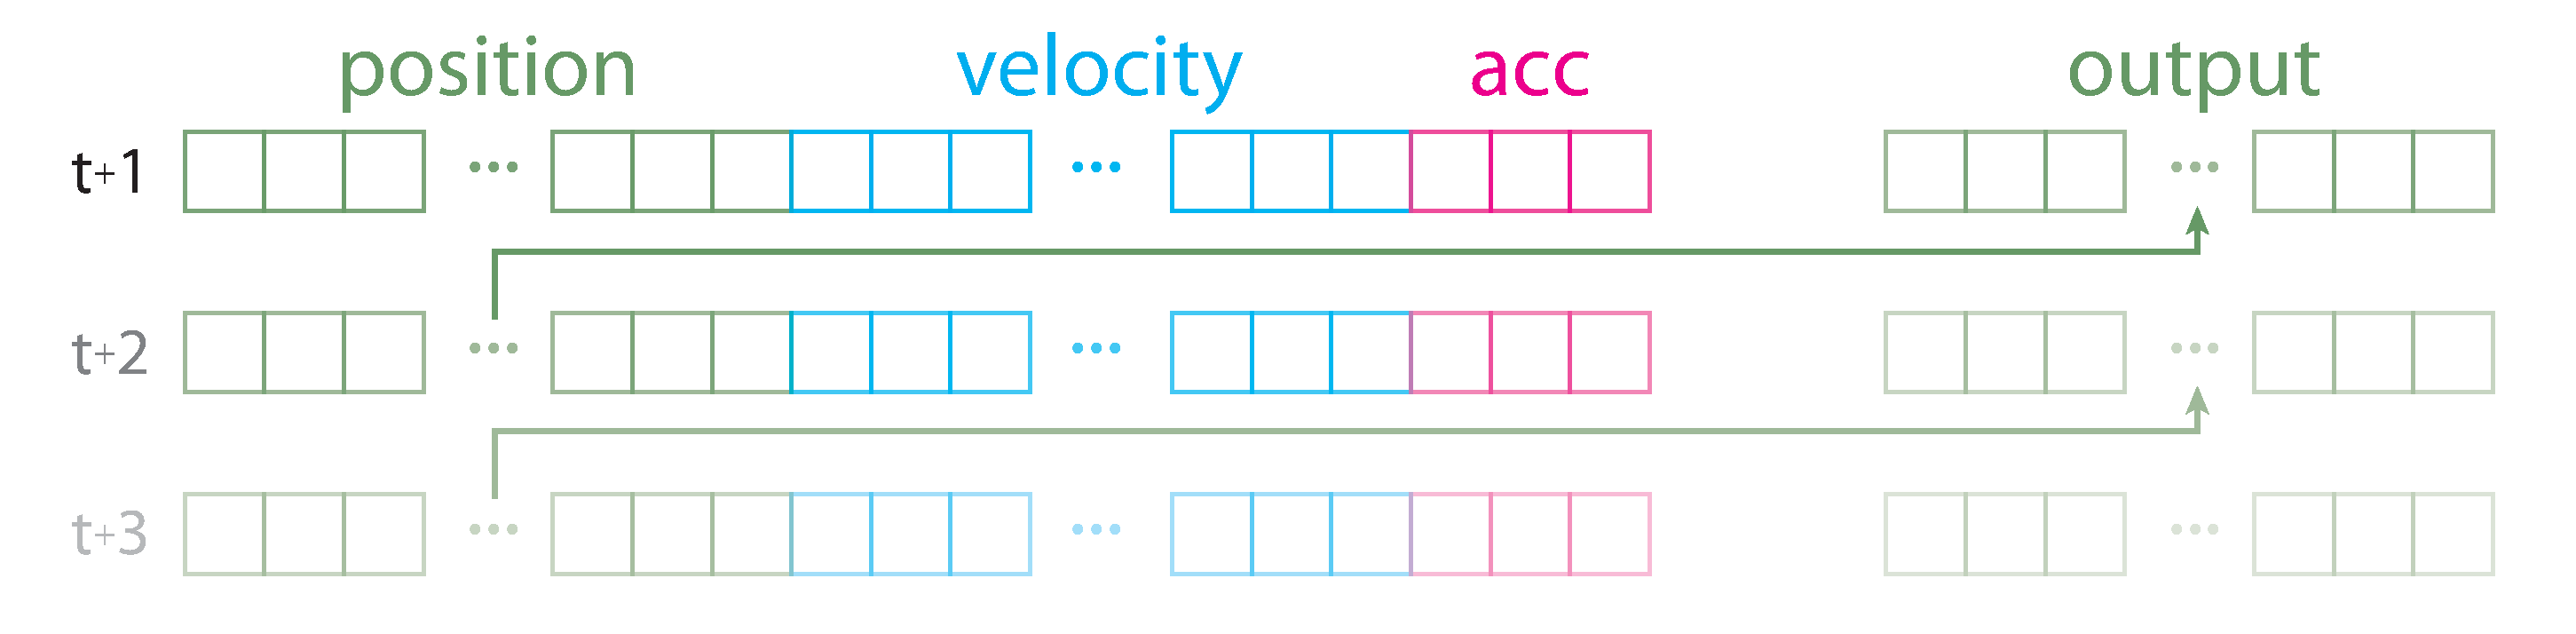
\includegraphics[width=\textwidth]{images/supervised/data2.pdf}
%\caption{Visualization of unrolled LSTM}
%\end{figure}


\subsection{Implementation, setup}
I have implemented a fully recurrent neural network using only python's native \textit{numpy} library used for matrix operations. The network was successfully able to mimic the training data, but the implementation itself was troublesome because every small change in the model (for example different activation) forced the whole backpropagation algorithm to change.

\medskip

I rewrote the net using the \textit{Theano} library which I picked for its complex symbolic differentiation capabilities. I constructed sort of a framework for neural networks, partially inspired by the \textit{keras} library. The 'framework' allowed me to construct networks of several neural layers by just specifying the sizes and types of layers consecutively.

The supported layers are:
\begin{itemize}
\item Fully connected (dense) layer
\item Fully recurrent layer
\item LSTM layer
\end{itemize}

The Theano library (and a few others - like tensorflow) simplify things greatly. Instead of working out the backpropagation updates by hand (or other means), it is only necessary to input symbolic matrix equations of the forward run and compute the gradient using the library's \textit{grad} function.

\medskip

When training the recurrent networks, I had a few different choices:
\begin{itemize}
\item \textbf{Backpropagation through time:} a straightforward learning technique, that unfolds the recurrent network in time by stacking identical copies of the RNN, and redirecting connections within the network to obtain connections between subsequent copies. This process creates a simple (but deep) feedforward network that allows for the use of the basic backpropagation algorithm.

\item \textbf{Limited BPTT:} The previous method however forces the network to unfold once for each time step. This is computationally unsustainable for longer sequences. A simple and commonly used variant of BPTT uses a finite history and limits the number of unfolds.

\item \textbf{Real-time recurrent learning:} RTRL is a gradient-descent method which computes the exact error gradient at every time step. The standard version of the algorithm has time complexity $O(n^4)$ \cite{cite:RTRL-complexity} (where $n$ is number of processing units in the network), which is quite high for effective implementation.
\end{itemize}

I chose Limited BPTT, because it supports efficient repeated batch learning (unlike BPTT and RTRL), needed for the reinforcement learning experiments.

\subsection{Network notation}
I will use the following notation (mimicking notation of the python 'framework') in the remainder of this thesis:

\begin{itemize}
\item \textbf{\{ \}:} basic network container
\item \textbf{\{\textit{i}, \textit{j}, ...\}:} each number represents a layer of stated size, the layers are connected in succession, the input and output layers are not explicitly mentioned
\item \textbf{\{lstm, rnn\}:} virtual recurrent layers, the input and output sizes are specified by sizes of the previous and next layer
\end{itemize}

An example net from figure \ref{fig:nn} would look like this: \{4, 3\}

Unless stated otherwise, the output layer has a tanh activation (to bound the output), hidden layers go through relu activation.

\subsection{Experiments}

The data itself are unfortunately quite limiting, because the recorded sequence is very short and after around 300 time steps it starts repeating itself. Because of this I couldn't use the usual train/validation/test splits and was unable to measure the model's performance by standard means. Instead I evaluated the learned nets on the robot itself, checking which models were able to walk.

I constructed several network architectures and retrained them repeatedly with different initial weights. Then I tested these networks on the robot itself, measuring the time and distance over several (10) runs. This was done to check the networks capability of overcoming the stochastic effects introduced by the simulator.

The nets used in the supervised experiments were the following:
\{\}, \{10\}, \{50\}, \{10, 10\}, \{50, 50\}, \{100, 100\}, \{lstm\}, \{lstm, 10\}, \{lstm, 100\}, \{rnn\}, \{rnn, 10\}, \{rnn, 100\}

This evaluation process is not entirely correct, because in the supervised learning setting, we are only fitting the provided data and the model doesn't know anything about the real walking task. However this was done mainly to test if the nets were even capable of walking and not to learn them to walk in the full extent.


\section{Conclusion}

About a quarter of the networks were capable of walking, however often at the cost of stability. Perhaps the most stable net still capable of walking was \{rnn, 10\}. The results and comparisons can be seen in figures \ref{plot:joints}, \ref{plot:joints2} and also in video~\ref{video:swingup}. For training details, see \ref{tab:supervised}.

\newpage

\begin{figure}[h!]
%% Creator: Matplotlib, PGF backend
%%
%% To include the figure in your LaTeX document, write
%%   \input{<filename>.pgf}
%%
%% Make sure the required packages are loaded in your preamble
%%   \usepackage{pgf}
%%
%% Figures using additional raster images can only be included by \input if
%% they are in the same directory as the main LaTeX file. For loading figures
%% from other directories you can use the `import` package
%%   \usepackage{import}
%% and then include the figures with
%%   \import{<path to file>}{<filename>.pgf}
%%
%% Matplotlib used the following preamble
%%   \usepackage[utf8x]{inputenc}
%%   \usepackage[T1]{fontenc}
%%
\begingroup%
\makeatletter%
\begin{pgfpicture}%
\pgfpathrectangle{\pgfpointorigin}{\pgfqpoint{5.022831in}{3.515982in}}%
\pgfusepath{use as bounding box, clip}%
\begin{pgfscope}%
\pgfsetbuttcap%
\pgfsetmiterjoin%
\definecolor{currentfill}{rgb}{1.000000,1.000000,1.000000}%
\pgfsetfillcolor{currentfill}%
\pgfsetlinewidth{0.000000pt}%
\definecolor{currentstroke}{rgb}{1.000000,1.000000,1.000000}%
\pgfsetstrokecolor{currentstroke}%
\pgfsetdash{}{0pt}%
\pgfpathmoveto{\pgfqpoint{0.000000in}{0.000000in}}%
\pgfpathlineto{\pgfqpoint{5.022831in}{0.000000in}}%
\pgfpathlineto{\pgfqpoint{5.022831in}{3.515982in}}%
\pgfpathlineto{\pgfqpoint{0.000000in}{3.515982in}}%
\pgfpathclose%
\pgfusepath{fill}%
\end{pgfscope}%
\begin{pgfscope}%
\pgfsetbuttcap%
\pgfsetmiterjoin%
\definecolor{currentfill}{rgb}{1.000000,1.000000,1.000000}%
\pgfsetfillcolor{currentfill}%
\pgfsetlinewidth{0.000000pt}%
\definecolor{currentstroke}{rgb}{0.000000,0.000000,0.000000}%
\pgfsetstrokecolor{currentstroke}%
\pgfsetstrokeopacity{0.000000}%
\pgfsetdash{}{0pt}%
\pgfpathmoveto{\pgfqpoint{0.448229in}{2.912771in}}%
\pgfpathlineto{\pgfqpoint{4.784288in}{2.912771in}}%
\pgfpathlineto{\pgfqpoint{4.784288in}{3.316920in}}%
\pgfpathlineto{\pgfqpoint{0.448229in}{3.316920in}}%
\pgfpathclose%
\pgfusepath{fill}%
\end{pgfscope}%
\begin{pgfscope}%
\pgfpathrectangle{\pgfqpoint{0.448229in}{2.912771in}}{\pgfqpoint{4.336059in}{0.404148in}} %
\pgfusepath{clip}%
\pgfsetrectcap%
\pgfsetroundjoin%
\pgfsetlinewidth{0.501875pt}%
\definecolor{currentstroke}{rgb}{0.000000,0.000000,1.000000}%
\pgfsetstrokecolor{currentstroke}%
\pgfsetdash{}{0pt}%
\pgfpathmoveto{\pgfqpoint{0.448229in}{3.074430in}}%
\pgfpathlineto{\pgfqpoint{1.055277in}{3.073527in}}%
\pgfpathlineto{\pgfqpoint{1.107310in}{3.071016in}}%
\pgfpathlineto{\pgfqpoint{1.159342in}{3.067476in}}%
\pgfpathlineto{\pgfqpoint{1.194031in}{3.063053in}}%
\pgfpathlineto{\pgfqpoint{1.280752in}{3.045030in}}%
\pgfpathlineto{\pgfqpoint{1.298096in}{3.043377in}}%
\pgfpathlineto{\pgfqpoint{1.315441in}{3.043509in}}%
\pgfpathlineto{\pgfqpoint{1.332785in}{3.047962in}}%
\pgfpathlineto{\pgfqpoint{1.350129in}{3.053994in}}%
\pgfpathlineto{\pgfqpoint{1.384818in}{3.069449in}}%
\pgfpathlineto{\pgfqpoint{1.402162in}{3.080246in}}%
\pgfpathlineto{\pgfqpoint{1.419506in}{3.076340in}}%
\pgfpathlineto{\pgfqpoint{1.436850in}{3.082083in}}%
\pgfpathlineto{\pgfqpoint{1.454195in}{3.084618in}}%
\pgfpathlineto{\pgfqpoint{1.471539in}{3.084719in}}%
\pgfpathlineto{\pgfqpoint{1.488883in}{3.082619in}}%
\pgfpathlineto{\pgfqpoint{1.506227in}{3.086214in}}%
\pgfpathlineto{\pgfqpoint{1.540916in}{3.070102in}}%
\pgfpathlineto{\pgfqpoint{1.592948in}{3.054183in}}%
\pgfpathlineto{\pgfqpoint{1.610293in}{3.053184in}}%
\pgfpathlineto{\pgfqpoint{1.627637in}{3.055854in}}%
\pgfpathlineto{\pgfqpoint{1.644981in}{3.060623in}}%
\pgfpathlineto{\pgfqpoint{1.662325in}{3.067125in}}%
\pgfpathlineto{\pgfqpoint{1.679670in}{3.076418in}}%
\pgfpathlineto{\pgfqpoint{1.697014in}{3.083852in}}%
\pgfpathlineto{\pgfqpoint{1.714358in}{3.078667in}}%
\pgfpathlineto{\pgfqpoint{1.731702in}{3.083824in}}%
\pgfpathlineto{\pgfqpoint{1.749047in}{3.086267in}}%
\pgfpathlineto{\pgfqpoint{1.766391in}{3.085384in}}%
\pgfpathlineto{\pgfqpoint{1.783735in}{3.083294in}}%
\pgfpathlineto{\pgfqpoint{1.801079in}{3.087152in}}%
\pgfpathlineto{\pgfqpoint{1.835768in}{3.069906in}}%
\pgfpathlineto{\pgfqpoint{1.853112in}{3.063037in}}%
\pgfpathlineto{\pgfqpoint{1.887800in}{3.052970in}}%
\pgfpathlineto{\pgfqpoint{1.905145in}{3.053088in}}%
\pgfpathlineto{\pgfqpoint{1.922489in}{3.055511in}}%
\pgfpathlineto{\pgfqpoint{1.939833in}{3.061570in}}%
\pgfpathlineto{\pgfqpoint{1.957177in}{3.069073in}}%
\pgfpathlineto{\pgfqpoint{1.974522in}{3.077868in}}%
\pgfpathlineto{\pgfqpoint{1.991866in}{3.084180in}}%
\pgfpathlineto{\pgfqpoint{2.009210in}{3.080629in}}%
\pgfpathlineto{\pgfqpoint{2.026554in}{3.084715in}}%
\pgfpathlineto{\pgfqpoint{2.043899in}{3.085850in}}%
\pgfpathlineto{\pgfqpoint{2.061243in}{3.084537in}}%
\pgfpathlineto{\pgfqpoint{2.095931in}{3.085167in}}%
\pgfpathlineto{\pgfqpoint{2.130620in}{3.067849in}}%
\pgfpathlineto{\pgfqpoint{2.147964in}{3.060761in}}%
\pgfpathlineto{\pgfqpoint{2.182653in}{3.052838in}}%
\pgfpathlineto{\pgfqpoint{2.199997in}{3.053281in}}%
\pgfpathlineto{\pgfqpoint{2.217341in}{3.057453in}}%
\pgfpathlineto{\pgfqpoint{2.234685in}{3.063104in}}%
\pgfpathlineto{\pgfqpoint{2.269374in}{3.078678in}}%
\pgfpathlineto{\pgfqpoint{2.286718in}{3.081002in}}%
\pgfpathlineto{\pgfqpoint{2.304062in}{3.079592in}}%
\pgfpathlineto{\pgfqpoint{2.321406in}{3.083488in}}%
\pgfpathlineto{\pgfqpoint{2.338751in}{3.083731in}}%
\pgfpathlineto{\pgfqpoint{2.356095in}{3.082676in}}%
\pgfpathlineto{\pgfqpoint{2.373439in}{3.084591in}}%
\pgfpathlineto{\pgfqpoint{2.390783in}{3.081985in}}%
\pgfpathlineto{\pgfqpoint{2.408128in}{3.072986in}}%
\pgfpathlineto{\pgfqpoint{2.425472in}{3.065614in}}%
\pgfpathlineto{\pgfqpoint{2.460160in}{3.054289in}}%
\pgfpathlineto{\pgfqpoint{2.477505in}{3.051526in}}%
\pgfpathlineto{\pgfqpoint{2.494849in}{3.052957in}}%
\pgfpathlineto{\pgfqpoint{2.512193in}{3.056535in}}%
\pgfpathlineto{\pgfqpoint{2.529537in}{3.063843in}}%
\pgfpathlineto{\pgfqpoint{2.546881in}{3.072572in}}%
\pgfpathlineto{\pgfqpoint{2.564226in}{3.079268in}}%
\pgfpathlineto{\pgfqpoint{2.581570in}{3.079351in}}%
\pgfpathlineto{\pgfqpoint{2.616258in}{3.083477in}}%
\pgfpathlineto{\pgfqpoint{2.633603in}{3.084524in}}%
\pgfpathlineto{\pgfqpoint{2.650947in}{3.082103in}}%
\pgfpathlineto{\pgfqpoint{2.668291in}{3.086950in}}%
\pgfpathlineto{\pgfqpoint{2.685635in}{3.081491in}}%
\pgfpathlineto{\pgfqpoint{2.702980in}{3.071456in}}%
\pgfpathlineto{\pgfqpoint{2.755012in}{3.055499in}}%
\pgfpathlineto{\pgfqpoint{2.772357in}{3.053690in}}%
\pgfpathlineto{\pgfqpoint{2.789701in}{3.055454in}}%
\pgfpathlineto{\pgfqpoint{2.807045in}{3.059742in}}%
\pgfpathlineto{\pgfqpoint{2.824389in}{3.066003in}}%
\pgfpathlineto{\pgfqpoint{2.859078in}{3.082754in}}%
\pgfpathlineto{\pgfqpoint{2.876422in}{3.078864in}}%
\pgfpathlineto{\pgfqpoint{2.893766in}{3.083294in}}%
\pgfpathlineto{\pgfqpoint{2.911110in}{3.085613in}}%
\pgfpathlineto{\pgfqpoint{2.928455in}{3.085710in}}%
\pgfpathlineto{\pgfqpoint{2.945799in}{3.083602in}}%
\pgfpathlineto{\pgfqpoint{2.963143in}{3.087198in}}%
\pgfpathlineto{\pgfqpoint{2.980487in}{3.081434in}}%
\pgfpathlineto{\pgfqpoint{3.015176in}{3.063228in}}%
\pgfpathlineto{\pgfqpoint{3.032520in}{3.056900in}}%
\pgfpathlineto{\pgfqpoint{3.049864in}{3.053474in}}%
\pgfpathlineto{\pgfqpoint{3.067209in}{3.051584in}}%
\pgfpathlineto{\pgfqpoint{3.101897in}{3.058635in}}%
\pgfpathlineto{\pgfqpoint{3.119241in}{3.065323in}}%
\pgfpathlineto{\pgfqpoint{3.136586in}{3.075857in}}%
\pgfpathlineto{\pgfqpoint{3.153930in}{3.081923in}}%
\pgfpathlineto{\pgfqpoint{3.171274in}{3.078608in}}%
\pgfpathlineto{\pgfqpoint{3.205963in}{3.084740in}}%
\pgfpathlineto{\pgfqpoint{3.223307in}{3.084085in}}%
\pgfpathlineto{\pgfqpoint{3.240651in}{3.082249in}}%
\pgfpathlineto{\pgfqpoint{3.257995in}{3.085783in}}%
\pgfpathlineto{\pgfqpoint{3.275339in}{3.075330in}}%
\pgfpathlineto{\pgfqpoint{3.292684in}{3.068540in}}%
\pgfpathlineto{\pgfqpoint{3.310028in}{3.060451in}}%
\pgfpathlineto{\pgfqpoint{3.344716in}{3.051694in}}%
\pgfpathlineto{\pgfqpoint{3.362061in}{3.052060in}}%
\pgfpathlineto{\pgfqpoint{3.379405in}{3.054630in}}%
\pgfpathlineto{\pgfqpoint{3.396749in}{3.060957in}}%
\pgfpathlineto{\pgfqpoint{3.431438in}{3.077711in}}%
\pgfpathlineto{\pgfqpoint{3.448782in}{3.082920in}}%
\pgfpathlineto{\pgfqpoint{3.466126in}{3.078675in}}%
\pgfpathlineto{\pgfqpoint{3.483470in}{3.081629in}}%
\pgfpathlineto{\pgfqpoint{3.500815in}{3.083250in}}%
\pgfpathlineto{\pgfqpoint{3.518159in}{3.082347in}}%
\pgfpathlineto{\pgfqpoint{3.552847in}{3.082930in}}%
\pgfpathlineto{\pgfqpoint{3.587536in}{3.066414in}}%
\pgfpathlineto{\pgfqpoint{3.622224in}{3.054624in}}%
\pgfpathlineto{\pgfqpoint{3.639568in}{3.051512in}}%
\pgfpathlineto{\pgfqpoint{3.656913in}{3.052255in}}%
\pgfpathlineto{\pgfqpoint{3.674257in}{3.056216in}}%
\pgfpathlineto{\pgfqpoint{3.691601in}{3.061868in}}%
\pgfpathlineto{\pgfqpoint{3.708945in}{3.069502in}}%
\pgfpathlineto{\pgfqpoint{3.726290in}{3.078621in}}%
\pgfpathlineto{\pgfqpoint{3.743634in}{3.082278in}}%
\pgfpathlineto{\pgfqpoint{3.760978in}{3.079721in}}%
\pgfpathlineto{\pgfqpoint{3.778322in}{3.082834in}}%
\pgfpathlineto{\pgfqpoint{3.795667in}{3.084360in}}%
\pgfpathlineto{\pgfqpoint{3.813011in}{3.083058in}}%
\pgfpathlineto{\pgfqpoint{3.830355in}{3.085632in}}%
\pgfpathlineto{\pgfqpoint{3.847699in}{3.083352in}}%
\pgfpathlineto{\pgfqpoint{3.865044in}{3.073038in}}%
\pgfpathlineto{\pgfqpoint{3.882388in}{3.065608in}}%
\pgfpathlineto{\pgfqpoint{3.917076in}{3.054750in}}%
\pgfpathlineto{\pgfqpoint{3.934420in}{3.053082in}}%
\pgfpathlineto{\pgfqpoint{3.951765in}{3.054747in}}%
\pgfpathlineto{\pgfqpoint{3.986453in}{3.063712in}}%
\pgfpathlineto{\pgfqpoint{4.003797in}{3.073928in}}%
\pgfpathlineto{\pgfqpoint{4.021142in}{3.082362in}}%
\pgfpathlineto{\pgfqpoint{4.038486in}{3.080721in}}%
\pgfpathlineto{\pgfqpoint{4.055830in}{3.081302in}}%
\pgfpathlineto{\pgfqpoint{4.073174in}{3.084538in}}%
\pgfpathlineto{\pgfqpoint{4.090519in}{3.085090in}}%
\pgfpathlineto{\pgfqpoint{4.107863in}{3.083185in}}%
\pgfpathlineto{\pgfqpoint{4.125207in}{3.087765in}}%
\pgfpathlineto{\pgfqpoint{4.177240in}{3.064022in}}%
\pgfpathlineto{\pgfqpoint{4.194584in}{3.059640in}}%
\pgfpathlineto{\pgfqpoint{4.211928in}{3.053934in}}%
\pgfpathlineto{\pgfqpoint{4.229273in}{3.052220in}}%
\pgfpathlineto{\pgfqpoint{4.263961in}{3.058525in}}%
\pgfpathlineto{\pgfqpoint{4.281305in}{3.064842in}}%
\pgfpathlineto{\pgfqpoint{4.298649in}{3.072951in}}%
\pgfpathlineto{\pgfqpoint{4.315994in}{3.082593in}}%
\pgfpathlineto{\pgfqpoint{4.333338in}{3.078890in}}%
\pgfpathlineto{\pgfqpoint{4.350682in}{3.082636in}}%
\pgfpathlineto{\pgfqpoint{4.368026in}{3.084396in}}%
\pgfpathlineto{\pgfqpoint{4.385371in}{3.084951in}}%
\pgfpathlineto{\pgfqpoint{4.402715in}{3.082229in}}%
\pgfpathlineto{\pgfqpoint{4.420059in}{3.086860in}}%
\pgfpathlineto{\pgfqpoint{4.489436in}{3.056707in}}%
\pgfpathlineto{\pgfqpoint{4.506780in}{3.052312in}}%
\pgfpathlineto{\pgfqpoint{4.524125in}{3.051354in}}%
\pgfpathlineto{\pgfqpoint{4.541469in}{3.054541in}}%
\pgfpathlineto{\pgfqpoint{4.576157in}{3.064642in}}%
\pgfpathlineto{\pgfqpoint{4.610846in}{3.083494in}}%
\pgfpathlineto{\pgfqpoint{4.628190in}{3.079164in}}%
\pgfpathlineto{\pgfqpoint{4.662878in}{3.085223in}}%
\pgfpathlineto{\pgfqpoint{4.680223in}{3.084515in}}%
\pgfpathlineto{\pgfqpoint{4.697567in}{3.082634in}}%
\pgfpathlineto{\pgfqpoint{4.714911in}{3.085754in}}%
\pgfpathlineto{\pgfqpoint{4.732255in}{3.078698in}}%
\pgfpathlineto{\pgfqpoint{4.749600in}{3.068043in}}%
\pgfpathlineto{\pgfqpoint{4.766944in}{3.061273in}}%
\pgfpathlineto{\pgfqpoint{4.766944in}{3.061273in}}%
\pgfusepath{stroke}%
\end{pgfscope}%
\begin{pgfscope}%
\pgfpathrectangle{\pgfqpoint{0.448229in}{2.912771in}}{\pgfqpoint{4.336059in}{0.404148in}} %
\pgfusepath{clip}%
\pgfsetrectcap%
\pgfsetroundjoin%
\pgfsetlinewidth{0.501875pt}%
\definecolor{currentstroke}{rgb}{0.000000,0.500000,0.000000}%
\pgfsetstrokecolor{currentstroke}%
\pgfsetdash{}{0pt}%
\pgfpathmoveto{\pgfqpoint{0.448229in}{3.074430in}}%
\pgfpathlineto{\pgfqpoint{1.055277in}{3.073527in}}%
\pgfpathlineto{\pgfqpoint{1.107310in}{3.071016in}}%
\pgfpathlineto{\pgfqpoint{1.159342in}{3.067476in}}%
\pgfpathlineto{\pgfqpoint{1.194031in}{3.063053in}}%
\pgfpathlineto{\pgfqpoint{1.263408in}{3.049701in}}%
\pgfpathlineto{\pgfqpoint{1.280752in}{3.056753in}}%
\pgfpathlineto{\pgfqpoint{1.315441in}{3.056422in}}%
\pgfpathlineto{\pgfqpoint{1.332785in}{3.058976in}}%
\pgfpathlineto{\pgfqpoint{1.350129in}{3.059627in}}%
\pgfpathlineto{\pgfqpoint{1.367473in}{3.061638in}}%
\pgfpathlineto{\pgfqpoint{1.384818in}{3.069449in}}%
\pgfpathlineto{\pgfqpoint{1.402162in}{3.080246in}}%
\pgfpathlineto{\pgfqpoint{1.436850in}{3.093636in}}%
\pgfpathlineto{\pgfqpoint{1.454195in}{3.096920in}}%
\pgfpathlineto{\pgfqpoint{1.471539in}{3.096158in}}%
\pgfpathlineto{\pgfqpoint{1.488883in}{3.092751in}}%
\pgfpathlineto{\pgfqpoint{1.523571in}{3.080226in}}%
\pgfpathlineto{\pgfqpoint{1.540916in}{3.070103in}}%
\pgfpathlineto{\pgfqpoint{1.558260in}{3.068020in}}%
\pgfpathlineto{\pgfqpoint{1.575604in}{3.069320in}}%
\pgfpathlineto{\pgfqpoint{1.592948in}{3.066217in}}%
\pgfpathlineto{\pgfqpoint{1.610293in}{3.064705in}}%
\pgfpathlineto{\pgfqpoint{1.627637in}{3.066262in}}%
\pgfpathlineto{\pgfqpoint{1.644981in}{3.063795in}}%
\pgfpathlineto{\pgfqpoint{1.662325in}{3.067125in}}%
\pgfpathlineto{\pgfqpoint{1.679670in}{3.076418in}}%
\pgfpathlineto{\pgfqpoint{1.697014in}{3.083852in}}%
\pgfpathlineto{\pgfqpoint{1.714358in}{3.088995in}}%
\pgfpathlineto{\pgfqpoint{1.731702in}{3.095558in}}%
\pgfpathlineto{\pgfqpoint{1.749047in}{3.098573in}}%
\pgfpathlineto{\pgfqpoint{1.783735in}{3.093027in}}%
\pgfpathlineto{\pgfqpoint{1.801079in}{3.087152in}}%
\pgfpathlineto{\pgfqpoint{1.835768in}{3.069906in}}%
\pgfpathlineto{\pgfqpoint{1.870456in}{3.068588in}}%
\pgfpathlineto{\pgfqpoint{1.887800in}{3.065164in}}%
\pgfpathlineto{\pgfqpoint{1.905145in}{3.064594in}}%
\pgfpathlineto{\pgfqpoint{1.922489in}{3.065906in}}%
\pgfpathlineto{\pgfqpoint{1.939833in}{3.062059in}}%
\pgfpathlineto{\pgfqpoint{1.957177in}{3.069073in}}%
\pgfpathlineto{\pgfqpoint{1.974522in}{3.077868in}}%
\pgfpathlineto{\pgfqpoint{2.026554in}{3.096906in}}%
\pgfpathlineto{\pgfqpoint{2.043899in}{3.098104in}}%
\pgfpathlineto{\pgfqpoint{2.078587in}{3.091565in}}%
\pgfpathlineto{\pgfqpoint{2.095931in}{3.085168in}}%
\pgfpathlineto{\pgfqpoint{2.130620in}{3.067849in}}%
\pgfpathlineto{\pgfqpoint{2.147964in}{3.071191in}}%
\pgfpathlineto{\pgfqpoint{2.182653in}{3.065041in}}%
\pgfpathlineto{\pgfqpoint{2.199997in}{3.064722in}}%
\pgfpathlineto{\pgfqpoint{2.217341in}{3.067430in}}%
\pgfpathlineto{\pgfqpoint{2.234685in}{3.063106in}}%
\pgfpathlineto{\pgfqpoint{2.286718in}{3.086574in}}%
\pgfpathlineto{\pgfqpoint{2.304062in}{3.090430in}}%
\pgfpathlineto{\pgfqpoint{2.321406in}{3.095671in}}%
\pgfpathlineto{\pgfqpoint{2.338751in}{3.095486in}}%
\pgfpathlineto{\pgfqpoint{2.356095in}{3.093135in}}%
\pgfpathlineto{\pgfqpoint{2.373439in}{3.088252in}}%
\pgfpathlineto{\pgfqpoint{2.390783in}{3.081986in}}%
\pgfpathlineto{\pgfqpoint{2.408128in}{3.072986in}}%
\pgfpathlineto{\pgfqpoint{2.425472in}{3.065614in}}%
\pgfpathlineto{\pgfqpoint{2.442816in}{3.069998in}}%
\pgfpathlineto{\pgfqpoint{2.460160in}{3.066074in}}%
\pgfpathlineto{\pgfqpoint{2.477505in}{3.063869in}}%
\pgfpathlineto{\pgfqpoint{2.494849in}{3.063904in}}%
\pgfpathlineto{\pgfqpoint{2.512193in}{3.066535in}}%
\pgfpathlineto{\pgfqpoint{2.529537in}{3.063845in}}%
\pgfpathlineto{\pgfqpoint{2.546881in}{3.072572in}}%
\pgfpathlineto{\pgfqpoint{2.564226in}{3.079268in}}%
\pgfpathlineto{\pgfqpoint{2.581570in}{3.087302in}}%
\pgfpathlineto{\pgfqpoint{2.598914in}{3.093161in}}%
\pgfpathlineto{\pgfqpoint{2.616258in}{3.095679in}}%
\pgfpathlineto{\pgfqpoint{2.633603in}{3.096178in}}%
\pgfpathlineto{\pgfqpoint{2.650947in}{3.092227in}}%
\pgfpathlineto{\pgfqpoint{2.685635in}{3.081490in}}%
\pgfpathlineto{\pgfqpoint{2.702980in}{3.071456in}}%
\pgfpathlineto{\pgfqpoint{2.720324in}{3.067227in}}%
\pgfpathlineto{\pgfqpoint{2.737668in}{3.071477in}}%
\pgfpathlineto{\pgfqpoint{2.755012in}{3.067248in}}%
\pgfpathlineto{\pgfqpoint{2.772357in}{3.065606in}}%
\pgfpathlineto{\pgfqpoint{2.807045in}{3.065897in}}%
\pgfpathlineto{\pgfqpoint{2.824389in}{3.066004in}}%
\pgfpathlineto{\pgfqpoint{2.859078in}{3.082754in}}%
\pgfpathlineto{\pgfqpoint{2.893766in}{3.094933in}}%
\pgfpathlineto{\pgfqpoint{2.911110in}{3.098036in}}%
\pgfpathlineto{\pgfqpoint{2.928455in}{3.096994in}}%
\pgfpathlineto{\pgfqpoint{2.945799in}{3.093802in}}%
\pgfpathlineto{\pgfqpoint{2.980487in}{3.081434in}}%
\pgfpathlineto{\pgfqpoint{2.997832in}{3.072249in}}%
\pgfpathlineto{\pgfqpoint{3.015176in}{3.068287in}}%
\pgfpathlineto{\pgfqpoint{3.032520in}{3.067954in}}%
\pgfpathlineto{\pgfqpoint{3.067209in}{3.063589in}}%
\pgfpathlineto{\pgfqpoint{3.084553in}{3.065599in}}%
\pgfpathlineto{\pgfqpoint{3.101897in}{3.063271in}}%
\pgfpathlineto{\pgfqpoint{3.119241in}{3.065324in}}%
\pgfpathlineto{\pgfqpoint{3.136586in}{3.075857in}}%
\pgfpathlineto{\pgfqpoint{3.153930in}{3.081923in}}%
\pgfpathlineto{\pgfqpoint{3.171274in}{3.089189in}}%
\pgfpathlineto{\pgfqpoint{3.205963in}{3.096827in}}%
\pgfpathlineto{\pgfqpoint{3.223307in}{3.095124in}}%
\pgfpathlineto{\pgfqpoint{3.240651in}{3.091207in}}%
\pgfpathlineto{\pgfqpoint{3.257995in}{3.085783in}}%
\pgfpathlineto{\pgfqpoint{3.275339in}{3.075330in}}%
\pgfpathlineto{\pgfqpoint{3.292684in}{3.068540in}}%
\pgfpathlineto{\pgfqpoint{3.327372in}{3.067318in}}%
\pgfpathlineto{\pgfqpoint{3.344716in}{3.064029in}}%
\pgfpathlineto{\pgfqpoint{3.362061in}{3.063620in}}%
\pgfpathlineto{\pgfqpoint{3.379405in}{3.065046in}}%
\pgfpathlineto{\pgfqpoint{3.396749in}{3.061201in}}%
\pgfpathlineto{\pgfqpoint{3.448782in}{3.083173in}}%
\pgfpathlineto{\pgfqpoint{3.466126in}{3.089402in}}%
\pgfpathlineto{\pgfqpoint{3.483470in}{3.093503in}}%
\pgfpathlineto{\pgfqpoint{3.500815in}{3.095178in}}%
\pgfpathlineto{\pgfqpoint{3.518159in}{3.092842in}}%
\pgfpathlineto{\pgfqpoint{3.535503in}{3.089192in}}%
\pgfpathlineto{\pgfqpoint{3.552847in}{3.082931in}}%
\pgfpathlineto{\pgfqpoint{3.587536in}{3.066414in}}%
\pgfpathlineto{\pgfqpoint{3.604880in}{3.069640in}}%
\pgfpathlineto{\pgfqpoint{3.622224in}{3.066145in}}%
\pgfpathlineto{\pgfqpoint{3.639568in}{3.063866in}}%
\pgfpathlineto{\pgfqpoint{3.656913in}{3.063595in}}%
\pgfpathlineto{\pgfqpoint{3.674257in}{3.066274in}}%
\pgfpathlineto{\pgfqpoint{3.691601in}{3.061869in}}%
\pgfpathlineto{\pgfqpoint{3.708945in}{3.069502in}}%
\pgfpathlineto{\pgfqpoint{3.726290in}{3.078621in}}%
\pgfpathlineto{\pgfqpoint{3.743634in}{3.084049in}}%
\pgfpathlineto{\pgfqpoint{3.760978in}{3.090660in}}%
\pgfpathlineto{\pgfqpoint{3.778322in}{3.094907in}}%
\pgfpathlineto{\pgfqpoint{3.795667in}{3.096310in}}%
\pgfpathlineto{\pgfqpoint{3.813011in}{3.093432in}}%
\pgfpathlineto{\pgfqpoint{3.847699in}{3.083353in}}%
\pgfpathlineto{\pgfqpoint{3.865044in}{3.073038in}}%
\pgfpathlineto{\pgfqpoint{3.882388in}{3.065608in}}%
\pgfpathlineto{\pgfqpoint{3.899732in}{3.070661in}}%
\pgfpathlineto{\pgfqpoint{3.917076in}{3.066542in}}%
\pgfpathlineto{\pgfqpoint{3.934420in}{3.065253in}}%
\pgfpathlineto{\pgfqpoint{3.969109in}{3.065698in}}%
\pgfpathlineto{\pgfqpoint{3.986453in}{3.063712in}}%
\pgfpathlineto{\pgfqpoint{4.003797in}{3.073928in}}%
\pgfpathlineto{\pgfqpoint{4.021142in}{3.082362in}}%
\pgfpathlineto{\pgfqpoint{4.073174in}{3.096838in}}%
\pgfpathlineto{\pgfqpoint{4.090519in}{3.096690in}}%
\pgfpathlineto{\pgfqpoint{4.107863in}{3.093415in}}%
\pgfpathlineto{\pgfqpoint{4.125207in}{3.088010in}}%
\pgfpathlineto{\pgfqpoint{4.159896in}{3.072883in}}%
\pgfpathlineto{\pgfqpoint{4.177240in}{3.066555in}}%
\pgfpathlineto{\pgfqpoint{4.194584in}{3.070173in}}%
\pgfpathlineto{\pgfqpoint{4.211928in}{3.065812in}}%
\pgfpathlineto{\pgfqpoint{4.229273in}{3.064167in}}%
\pgfpathlineto{\pgfqpoint{4.246617in}{3.065682in}}%
\pgfpathlineto{\pgfqpoint{4.281305in}{3.064843in}}%
\pgfpathlineto{\pgfqpoint{4.298649in}{3.072951in}}%
\pgfpathlineto{\pgfqpoint{4.315994in}{3.082593in}}%
\pgfpathlineto{\pgfqpoint{4.333338in}{3.087360in}}%
\pgfpathlineto{\pgfqpoint{4.350682in}{3.094351in}}%
\pgfpathlineto{\pgfqpoint{4.368026in}{3.096678in}}%
\pgfpathlineto{\pgfqpoint{4.385371in}{3.096269in}}%
\pgfpathlineto{\pgfqpoint{4.402715in}{3.092284in}}%
\pgfpathlineto{\pgfqpoint{4.420059in}{3.086862in}}%
\pgfpathlineto{\pgfqpoint{4.454748in}{3.071759in}}%
\pgfpathlineto{\pgfqpoint{4.472092in}{3.067092in}}%
\pgfpathlineto{\pgfqpoint{4.489436in}{3.067714in}}%
\pgfpathlineto{\pgfqpoint{4.506780in}{3.064570in}}%
\pgfpathlineto{\pgfqpoint{4.524125in}{3.063227in}}%
\pgfpathlineto{\pgfqpoint{4.541469in}{3.064962in}}%
\pgfpathlineto{\pgfqpoint{4.558813in}{3.062322in}}%
\pgfpathlineto{\pgfqpoint{4.576157in}{3.064642in}}%
\pgfpathlineto{\pgfqpoint{4.610846in}{3.083495in}}%
\pgfpathlineto{\pgfqpoint{4.628190in}{3.089732in}}%
\pgfpathlineto{\pgfqpoint{4.662878in}{3.097371in}}%
\pgfpathlineto{\pgfqpoint{4.680223in}{3.095581in}}%
\pgfpathlineto{\pgfqpoint{4.697567in}{3.091593in}}%
\pgfpathlineto{\pgfqpoint{4.714911in}{3.085753in}}%
\pgfpathlineto{\pgfqpoint{4.732255in}{3.078697in}}%
\pgfpathlineto{\pgfqpoint{4.749600in}{3.068043in}}%
\pgfpathlineto{\pgfqpoint{4.766944in}{3.068284in}}%
\pgfpathlineto{\pgfqpoint{4.766944in}{3.068284in}}%
\pgfusepath{stroke}%
\end{pgfscope}%
\begin{pgfscope}%
\pgfsetrectcap%
\pgfsetmiterjoin%
\pgfsetlinewidth{1.003750pt}%
\definecolor{currentstroke}{rgb}{0.000000,0.000000,0.000000}%
\pgfsetstrokecolor{currentstroke}%
\pgfsetdash{}{0pt}%
\pgfpathmoveto{\pgfqpoint{0.448229in}{3.316920in}}%
\pgfpathlineto{\pgfqpoint{4.784288in}{3.316920in}}%
\pgfusepath{stroke}%
\end{pgfscope}%
\begin{pgfscope}%
\pgfsetrectcap%
\pgfsetmiterjoin%
\pgfsetlinewidth{1.003750pt}%
\definecolor{currentstroke}{rgb}{0.000000,0.000000,0.000000}%
\pgfsetstrokecolor{currentstroke}%
\pgfsetdash{}{0pt}%
\pgfpathmoveto{\pgfqpoint{4.784288in}{2.912771in}}%
\pgfpathlineto{\pgfqpoint{4.784288in}{3.316920in}}%
\pgfusepath{stroke}%
\end{pgfscope}%
\begin{pgfscope}%
\pgfsetrectcap%
\pgfsetmiterjoin%
\pgfsetlinewidth{1.003750pt}%
\definecolor{currentstroke}{rgb}{0.000000,0.000000,0.000000}%
\pgfsetstrokecolor{currentstroke}%
\pgfsetdash{}{0pt}%
\pgfpathmoveto{\pgfqpoint{0.448229in}{2.912771in}}%
\pgfpathlineto{\pgfqpoint{4.784288in}{2.912771in}}%
\pgfusepath{stroke}%
\end{pgfscope}%
\begin{pgfscope}%
\pgfsetrectcap%
\pgfsetmiterjoin%
\pgfsetlinewidth{1.003750pt}%
\definecolor{currentstroke}{rgb}{0.000000,0.000000,0.000000}%
\pgfsetstrokecolor{currentstroke}%
\pgfsetdash{}{0pt}%
\pgfpathmoveto{\pgfqpoint{0.448229in}{2.912771in}}%
\pgfpathlineto{\pgfqpoint{0.448229in}{3.316920in}}%
\pgfusepath{stroke}%
\end{pgfscope}%
\begin{pgfscope}%
\pgfpathrectangle{\pgfqpoint{0.448229in}{2.912771in}}{\pgfqpoint{4.336059in}{0.404148in}} %
\pgfusepath{clip}%
\pgfsetbuttcap%
\pgfsetroundjoin%
\pgfsetlinewidth{0.501875pt}%
\definecolor{currentstroke}{rgb}{0.000000,0.000000,0.000000}%
\pgfsetstrokecolor{currentstroke}%
\pgfsetdash{{1.000000pt}{3.000000pt}}{0.000000pt}%
\pgfpathmoveto{\pgfqpoint{0.448229in}{2.912771in}}%
\pgfpathlineto{\pgfqpoint{0.448229in}{3.316920in}}%
\pgfusepath{stroke}%
\end{pgfscope}%
\begin{pgfscope}%
\pgfsetbuttcap%
\pgfsetroundjoin%
\definecolor{currentfill}{rgb}{0.000000,0.000000,0.000000}%
\pgfsetfillcolor{currentfill}%
\pgfsetlinewidth{0.501875pt}%
\definecolor{currentstroke}{rgb}{0.000000,0.000000,0.000000}%
\pgfsetstrokecolor{currentstroke}%
\pgfsetdash{}{0pt}%
\pgfsys@defobject{currentmarker}{\pgfqpoint{0.000000in}{0.000000in}}{\pgfqpoint{0.000000in}{0.055556in}}{%
\pgfpathmoveto{\pgfqpoint{0.000000in}{0.000000in}}%
\pgfpathlineto{\pgfqpoint{0.000000in}{0.055556in}}%
\pgfusepath{stroke,fill}%
}%
\begin{pgfscope}%
\pgfsys@transformshift{0.448229in}{2.912771in}%
\pgfsys@useobject{currentmarker}{}%
\end{pgfscope}%
\end{pgfscope}%
\begin{pgfscope}%
\pgfsetbuttcap%
\pgfsetroundjoin%
\definecolor{currentfill}{rgb}{0.000000,0.000000,0.000000}%
\pgfsetfillcolor{currentfill}%
\pgfsetlinewidth{0.501875pt}%
\definecolor{currentstroke}{rgb}{0.000000,0.000000,0.000000}%
\pgfsetstrokecolor{currentstroke}%
\pgfsetdash{}{0pt}%
\pgfsys@defobject{currentmarker}{\pgfqpoint{0.000000in}{-0.055556in}}{\pgfqpoint{0.000000in}{0.000000in}}{%
\pgfpathmoveto{\pgfqpoint{0.000000in}{0.000000in}}%
\pgfpathlineto{\pgfqpoint{0.000000in}{-0.055556in}}%
\pgfusepath{stroke,fill}%
}%
\begin{pgfscope}%
\pgfsys@transformshift{0.448229in}{3.316920in}%
\pgfsys@useobject{currentmarker}{}%
\end{pgfscope}%
\end{pgfscope}%
\begin{pgfscope}%
\pgfpathrectangle{\pgfqpoint{0.448229in}{2.912771in}}{\pgfqpoint{4.336059in}{0.404148in}} %
\pgfusepath{clip}%
\pgfsetbuttcap%
\pgfsetroundjoin%
\pgfsetlinewidth{0.501875pt}%
\definecolor{currentstroke}{rgb}{0.000000,0.000000,0.000000}%
\pgfsetstrokecolor{currentstroke}%
\pgfsetdash{{1.000000pt}{3.000000pt}}{0.000000pt}%
\pgfpathmoveto{\pgfqpoint{1.315441in}{2.912771in}}%
\pgfpathlineto{\pgfqpoint{1.315441in}{3.316920in}}%
\pgfusepath{stroke}%
\end{pgfscope}%
\begin{pgfscope}%
\pgfsetbuttcap%
\pgfsetroundjoin%
\definecolor{currentfill}{rgb}{0.000000,0.000000,0.000000}%
\pgfsetfillcolor{currentfill}%
\pgfsetlinewidth{0.501875pt}%
\definecolor{currentstroke}{rgb}{0.000000,0.000000,0.000000}%
\pgfsetstrokecolor{currentstroke}%
\pgfsetdash{}{0pt}%
\pgfsys@defobject{currentmarker}{\pgfqpoint{0.000000in}{0.000000in}}{\pgfqpoint{0.000000in}{0.055556in}}{%
\pgfpathmoveto{\pgfqpoint{0.000000in}{0.000000in}}%
\pgfpathlineto{\pgfqpoint{0.000000in}{0.055556in}}%
\pgfusepath{stroke,fill}%
}%
\begin{pgfscope}%
\pgfsys@transformshift{1.315441in}{2.912771in}%
\pgfsys@useobject{currentmarker}{}%
\end{pgfscope}%
\end{pgfscope}%
\begin{pgfscope}%
\pgfsetbuttcap%
\pgfsetroundjoin%
\definecolor{currentfill}{rgb}{0.000000,0.000000,0.000000}%
\pgfsetfillcolor{currentfill}%
\pgfsetlinewidth{0.501875pt}%
\definecolor{currentstroke}{rgb}{0.000000,0.000000,0.000000}%
\pgfsetstrokecolor{currentstroke}%
\pgfsetdash{}{0pt}%
\pgfsys@defobject{currentmarker}{\pgfqpoint{0.000000in}{-0.055556in}}{\pgfqpoint{0.000000in}{0.000000in}}{%
\pgfpathmoveto{\pgfqpoint{0.000000in}{0.000000in}}%
\pgfpathlineto{\pgfqpoint{0.000000in}{-0.055556in}}%
\pgfusepath{stroke,fill}%
}%
\begin{pgfscope}%
\pgfsys@transformshift{1.315441in}{3.316920in}%
\pgfsys@useobject{currentmarker}{}%
\end{pgfscope}%
\end{pgfscope}%
\begin{pgfscope}%
\pgfpathrectangle{\pgfqpoint{0.448229in}{2.912771in}}{\pgfqpoint{4.336059in}{0.404148in}} %
\pgfusepath{clip}%
\pgfsetbuttcap%
\pgfsetroundjoin%
\pgfsetlinewidth{0.501875pt}%
\definecolor{currentstroke}{rgb}{0.000000,0.000000,0.000000}%
\pgfsetstrokecolor{currentstroke}%
\pgfsetdash{{1.000000pt}{3.000000pt}}{0.000000pt}%
\pgfpathmoveto{\pgfqpoint{2.182653in}{2.912771in}}%
\pgfpathlineto{\pgfqpoint{2.182653in}{3.316920in}}%
\pgfusepath{stroke}%
\end{pgfscope}%
\begin{pgfscope}%
\pgfsetbuttcap%
\pgfsetroundjoin%
\definecolor{currentfill}{rgb}{0.000000,0.000000,0.000000}%
\pgfsetfillcolor{currentfill}%
\pgfsetlinewidth{0.501875pt}%
\definecolor{currentstroke}{rgb}{0.000000,0.000000,0.000000}%
\pgfsetstrokecolor{currentstroke}%
\pgfsetdash{}{0pt}%
\pgfsys@defobject{currentmarker}{\pgfqpoint{0.000000in}{0.000000in}}{\pgfqpoint{0.000000in}{0.055556in}}{%
\pgfpathmoveto{\pgfqpoint{0.000000in}{0.000000in}}%
\pgfpathlineto{\pgfqpoint{0.000000in}{0.055556in}}%
\pgfusepath{stroke,fill}%
}%
\begin{pgfscope}%
\pgfsys@transformshift{2.182653in}{2.912771in}%
\pgfsys@useobject{currentmarker}{}%
\end{pgfscope}%
\end{pgfscope}%
\begin{pgfscope}%
\pgfsetbuttcap%
\pgfsetroundjoin%
\definecolor{currentfill}{rgb}{0.000000,0.000000,0.000000}%
\pgfsetfillcolor{currentfill}%
\pgfsetlinewidth{0.501875pt}%
\definecolor{currentstroke}{rgb}{0.000000,0.000000,0.000000}%
\pgfsetstrokecolor{currentstroke}%
\pgfsetdash{}{0pt}%
\pgfsys@defobject{currentmarker}{\pgfqpoint{0.000000in}{-0.055556in}}{\pgfqpoint{0.000000in}{0.000000in}}{%
\pgfpathmoveto{\pgfqpoint{0.000000in}{0.000000in}}%
\pgfpathlineto{\pgfqpoint{0.000000in}{-0.055556in}}%
\pgfusepath{stroke,fill}%
}%
\begin{pgfscope}%
\pgfsys@transformshift{2.182653in}{3.316920in}%
\pgfsys@useobject{currentmarker}{}%
\end{pgfscope}%
\end{pgfscope}%
\begin{pgfscope}%
\pgfpathrectangle{\pgfqpoint{0.448229in}{2.912771in}}{\pgfqpoint{4.336059in}{0.404148in}} %
\pgfusepath{clip}%
\pgfsetbuttcap%
\pgfsetroundjoin%
\pgfsetlinewidth{0.501875pt}%
\definecolor{currentstroke}{rgb}{0.000000,0.000000,0.000000}%
\pgfsetstrokecolor{currentstroke}%
\pgfsetdash{{1.000000pt}{3.000000pt}}{0.000000pt}%
\pgfpathmoveto{\pgfqpoint{3.049864in}{2.912771in}}%
\pgfpathlineto{\pgfqpoint{3.049864in}{3.316920in}}%
\pgfusepath{stroke}%
\end{pgfscope}%
\begin{pgfscope}%
\pgfsetbuttcap%
\pgfsetroundjoin%
\definecolor{currentfill}{rgb}{0.000000,0.000000,0.000000}%
\pgfsetfillcolor{currentfill}%
\pgfsetlinewidth{0.501875pt}%
\definecolor{currentstroke}{rgb}{0.000000,0.000000,0.000000}%
\pgfsetstrokecolor{currentstroke}%
\pgfsetdash{}{0pt}%
\pgfsys@defobject{currentmarker}{\pgfqpoint{0.000000in}{0.000000in}}{\pgfqpoint{0.000000in}{0.055556in}}{%
\pgfpathmoveto{\pgfqpoint{0.000000in}{0.000000in}}%
\pgfpathlineto{\pgfqpoint{0.000000in}{0.055556in}}%
\pgfusepath{stroke,fill}%
}%
\begin{pgfscope}%
\pgfsys@transformshift{3.049864in}{2.912771in}%
\pgfsys@useobject{currentmarker}{}%
\end{pgfscope}%
\end{pgfscope}%
\begin{pgfscope}%
\pgfsetbuttcap%
\pgfsetroundjoin%
\definecolor{currentfill}{rgb}{0.000000,0.000000,0.000000}%
\pgfsetfillcolor{currentfill}%
\pgfsetlinewidth{0.501875pt}%
\definecolor{currentstroke}{rgb}{0.000000,0.000000,0.000000}%
\pgfsetstrokecolor{currentstroke}%
\pgfsetdash{}{0pt}%
\pgfsys@defobject{currentmarker}{\pgfqpoint{0.000000in}{-0.055556in}}{\pgfqpoint{0.000000in}{0.000000in}}{%
\pgfpathmoveto{\pgfqpoint{0.000000in}{0.000000in}}%
\pgfpathlineto{\pgfqpoint{0.000000in}{-0.055556in}}%
\pgfusepath{stroke,fill}%
}%
\begin{pgfscope}%
\pgfsys@transformshift{3.049864in}{3.316920in}%
\pgfsys@useobject{currentmarker}{}%
\end{pgfscope}%
\end{pgfscope}%
\begin{pgfscope}%
\pgfpathrectangle{\pgfqpoint{0.448229in}{2.912771in}}{\pgfqpoint{4.336059in}{0.404148in}} %
\pgfusepath{clip}%
\pgfsetbuttcap%
\pgfsetroundjoin%
\pgfsetlinewidth{0.501875pt}%
\definecolor{currentstroke}{rgb}{0.000000,0.000000,0.000000}%
\pgfsetstrokecolor{currentstroke}%
\pgfsetdash{{1.000000pt}{3.000000pt}}{0.000000pt}%
\pgfpathmoveto{\pgfqpoint{3.917076in}{2.912771in}}%
\pgfpathlineto{\pgfqpoint{3.917076in}{3.316920in}}%
\pgfusepath{stroke}%
\end{pgfscope}%
\begin{pgfscope}%
\pgfsetbuttcap%
\pgfsetroundjoin%
\definecolor{currentfill}{rgb}{0.000000,0.000000,0.000000}%
\pgfsetfillcolor{currentfill}%
\pgfsetlinewidth{0.501875pt}%
\definecolor{currentstroke}{rgb}{0.000000,0.000000,0.000000}%
\pgfsetstrokecolor{currentstroke}%
\pgfsetdash{}{0pt}%
\pgfsys@defobject{currentmarker}{\pgfqpoint{0.000000in}{0.000000in}}{\pgfqpoint{0.000000in}{0.055556in}}{%
\pgfpathmoveto{\pgfqpoint{0.000000in}{0.000000in}}%
\pgfpathlineto{\pgfqpoint{0.000000in}{0.055556in}}%
\pgfusepath{stroke,fill}%
}%
\begin{pgfscope}%
\pgfsys@transformshift{3.917076in}{2.912771in}%
\pgfsys@useobject{currentmarker}{}%
\end{pgfscope}%
\end{pgfscope}%
\begin{pgfscope}%
\pgfsetbuttcap%
\pgfsetroundjoin%
\definecolor{currentfill}{rgb}{0.000000,0.000000,0.000000}%
\pgfsetfillcolor{currentfill}%
\pgfsetlinewidth{0.501875pt}%
\definecolor{currentstroke}{rgb}{0.000000,0.000000,0.000000}%
\pgfsetstrokecolor{currentstroke}%
\pgfsetdash{}{0pt}%
\pgfsys@defobject{currentmarker}{\pgfqpoint{0.000000in}{-0.055556in}}{\pgfqpoint{0.000000in}{0.000000in}}{%
\pgfpathmoveto{\pgfqpoint{0.000000in}{0.000000in}}%
\pgfpathlineto{\pgfqpoint{0.000000in}{-0.055556in}}%
\pgfusepath{stroke,fill}%
}%
\begin{pgfscope}%
\pgfsys@transformshift{3.917076in}{3.316920in}%
\pgfsys@useobject{currentmarker}{}%
\end{pgfscope}%
\end{pgfscope}%
\begin{pgfscope}%
\pgfpathrectangle{\pgfqpoint{0.448229in}{2.912771in}}{\pgfqpoint{4.336059in}{0.404148in}} %
\pgfusepath{clip}%
\pgfsetbuttcap%
\pgfsetroundjoin%
\pgfsetlinewidth{0.501875pt}%
\definecolor{currentstroke}{rgb}{0.000000,0.000000,0.000000}%
\pgfsetstrokecolor{currentstroke}%
\pgfsetdash{{1.000000pt}{3.000000pt}}{0.000000pt}%
\pgfpathmoveto{\pgfqpoint{4.784288in}{2.912771in}}%
\pgfpathlineto{\pgfqpoint{4.784288in}{3.316920in}}%
\pgfusepath{stroke}%
\end{pgfscope}%
\begin{pgfscope}%
\pgfsetbuttcap%
\pgfsetroundjoin%
\definecolor{currentfill}{rgb}{0.000000,0.000000,0.000000}%
\pgfsetfillcolor{currentfill}%
\pgfsetlinewidth{0.501875pt}%
\definecolor{currentstroke}{rgb}{0.000000,0.000000,0.000000}%
\pgfsetstrokecolor{currentstroke}%
\pgfsetdash{}{0pt}%
\pgfsys@defobject{currentmarker}{\pgfqpoint{0.000000in}{0.000000in}}{\pgfqpoint{0.000000in}{0.055556in}}{%
\pgfpathmoveto{\pgfqpoint{0.000000in}{0.000000in}}%
\pgfpathlineto{\pgfqpoint{0.000000in}{0.055556in}}%
\pgfusepath{stroke,fill}%
}%
\begin{pgfscope}%
\pgfsys@transformshift{4.784288in}{2.912771in}%
\pgfsys@useobject{currentmarker}{}%
\end{pgfscope}%
\end{pgfscope}%
\begin{pgfscope}%
\pgfsetbuttcap%
\pgfsetroundjoin%
\definecolor{currentfill}{rgb}{0.000000,0.000000,0.000000}%
\pgfsetfillcolor{currentfill}%
\pgfsetlinewidth{0.501875pt}%
\definecolor{currentstroke}{rgb}{0.000000,0.000000,0.000000}%
\pgfsetstrokecolor{currentstroke}%
\pgfsetdash{}{0pt}%
\pgfsys@defobject{currentmarker}{\pgfqpoint{0.000000in}{-0.055556in}}{\pgfqpoint{0.000000in}{0.000000in}}{%
\pgfpathmoveto{\pgfqpoint{0.000000in}{0.000000in}}%
\pgfpathlineto{\pgfqpoint{0.000000in}{-0.055556in}}%
\pgfusepath{stroke,fill}%
}%
\begin{pgfscope}%
\pgfsys@transformshift{4.784288in}{3.316920in}%
\pgfsys@useobject{currentmarker}{}%
\end{pgfscope}%
\end{pgfscope}%
\begin{pgfscope}%
\pgfpathrectangle{\pgfqpoint{0.448229in}{2.912771in}}{\pgfqpoint{4.336059in}{0.404148in}} %
\pgfusepath{clip}%
\pgfsetbuttcap%
\pgfsetroundjoin%
\pgfsetlinewidth{0.501875pt}%
\definecolor{currentstroke}{rgb}{0.000000,0.000000,0.000000}%
\pgfsetstrokecolor{currentstroke}%
\pgfsetdash{{1.000000pt}{3.000000pt}}{0.000000pt}%
\pgfpathmoveto{\pgfqpoint{0.448229in}{2.912771in}}%
\pgfpathlineto{\pgfqpoint{4.784288in}{2.912771in}}%
\pgfusepath{stroke}%
\end{pgfscope}%
\begin{pgfscope}%
\pgfsetbuttcap%
\pgfsetroundjoin%
\definecolor{currentfill}{rgb}{0.000000,0.000000,0.000000}%
\pgfsetfillcolor{currentfill}%
\pgfsetlinewidth{0.501875pt}%
\definecolor{currentstroke}{rgb}{0.000000,0.000000,0.000000}%
\pgfsetstrokecolor{currentstroke}%
\pgfsetdash{}{0pt}%
\pgfsys@defobject{currentmarker}{\pgfqpoint{0.000000in}{0.000000in}}{\pgfqpoint{0.055556in}{0.000000in}}{%
\pgfpathmoveto{\pgfqpoint{0.000000in}{0.000000in}}%
\pgfpathlineto{\pgfqpoint{0.055556in}{0.000000in}}%
\pgfusepath{stroke,fill}%
}%
\begin{pgfscope}%
\pgfsys@transformshift{0.448229in}{2.912771in}%
\pgfsys@useobject{currentmarker}{}%
\end{pgfscope}%
\end{pgfscope}%
\begin{pgfscope}%
\pgfsetbuttcap%
\pgfsetroundjoin%
\definecolor{currentfill}{rgb}{0.000000,0.000000,0.000000}%
\pgfsetfillcolor{currentfill}%
\pgfsetlinewidth{0.501875pt}%
\definecolor{currentstroke}{rgb}{0.000000,0.000000,0.000000}%
\pgfsetstrokecolor{currentstroke}%
\pgfsetdash{}{0pt}%
\pgfsys@defobject{currentmarker}{\pgfqpoint{-0.055556in}{0.000000in}}{\pgfqpoint{0.000000in}{0.000000in}}{%
\pgfpathmoveto{\pgfqpoint{0.000000in}{0.000000in}}%
\pgfpathlineto{\pgfqpoint{-0.055556in}{0.000000in}}%
\pgfusepath{stroke,fill}%
}%
\begin{pgfscope}%
\pgfsys@transformshift{4.784288in}{2.912771in}%
\pgfsys@useobject{currentmarker}{}%
\end{pgfscope}%
\end{pgfscope}%
\begin{pgfscope}%
\pgftext[x=0.392673in,y=2.912771in,right,]{\fontsize{8.000000}{9.600000}\selectfont \(\displaystyle -1.0\)}%
\end{pgfscope}%
\begin{pgfscope}%
\pgfpathrectangle{\pgfqpoint{0.448229in}{2.912771in}}{\pgfqpoint{4.336059in}{0.404148in}} %
\pgfusepath{clip}%
\pgfsetbuttcap%
\pgfsetroundjoin%
\pgfsetlinewidth{0.501875pt}%
\definecolor{currentstroke}{rgb}{0.000000,0.000000,0.000000}%
\pgfsetstrokecolor{currentstroke}%
\pgfsetdash{{1.000000pt}{3.000000pt}}{0.000000pt}%
\pgfpathmoveto{\pgfqpoint{0.448229in}{2.993601in}}%
\pgfpathlineto{\pgfqpoint{4.784288in}{2.993601in}}%
\pgfusepath{stroke}%
\end{pgfscope}%
\begin{pgfscope}%
\pgfsetbuttcap%
\pgfsetroundjoin%
\definecolor{currentfill}{rgb}{0.000000,0.000000,0.000000}%
\pgfsetfillcolor{currentfill}%
\pgfsetlinewidth{0.501875pt}%
\definecolor{currentstroke}{rgb}{0.000000,0.000000,0.000000}%
\pgfsetstrokecolor{currentstroke}%
\pgfsetdash{}{0pt}%
\pgfsys@defobject{currentmarker}{\pgfqpoint{0.000000in}{0.000000in}}{\pgfqpoint{0.055556in}{0.000000in}}{%
\pgfpathmoveto{\pgfqpoint{0.000000in}{0.000000in}}%
\pgfpathlineto{\pgfqpoint{0.055556in}{0.000000in}}%
\pgfusepath{stroke,fill}%
}%
\begin{pgfscope}%
\pgfsys@transformshift{0.448229in}{2.993601in}%
\pgfsys@useobject{currentmarker}{}%
\end{pgfscope}%
\end{pgfscope}%
\begin{pgfscope}%
\pgfsetbuttcap%
\pgfsetroundjoin%
\definecolor{currentfill}{rgb}{0.000000,0.000000,0.000000}%
\pgfsetfillcolor{currentfill}%
\pgfsetlinewidth{0.501875pt}%
\definecolor{currentstroke}{rgb}{0.000000,0.000000,0.000000}%
\pgfsetstrokecolor{currentstroke}%
\pgfsetdash{}{0pt}%
\pgfsys@defobject{currentmarker}{\pgfqpoint{-0.055556in}{0.000000in}}{\pgfqpoint{0.000000in}{0.000000in}}{%
\pgfpathmoveto{\pgfqpoint{0.000000in}{0.000000in}}%
\pgfpathlineto{\pgfqpoint{-0.055556in}{0.000000in}}%
\pgfusepath{stroke,fill}%
}%
\begin{pgfscope}%
\pgfsys@transformshift{4.784288in}{2.993601in}%
\pgfsys@useobject{currentmarker}{}%
\end{pgfscope}%
\end{pgfscope}%
\begin{pgfscope}%
\pgftext[x=0.392673in,y=2.993601in,right,]{\fontsize{8.000000}{9.600000}\selectfont \(\displaystyle -0.5\)}%
\end{pgfscope}%
\begin{pgfscope}%
\pgfpathrectangle{\pgfqpoint{0.448229in}{2.912771in}}{\pgfqpoint{4.336059in}{0.404148in}} %
\pgfusepath{clip}%
\pgfsetbuttcap%
\pgfsetroundjoin%
\pgfsetlinewidth{0.501875pt}%
\definecolor{currentstroke}{rgb}{0.000000,0.000000,0.000000}%
\pgfsetstrokecolor{currentstroke}%
\pgfsetdash{{1.000000pt}{3.000000pt}}{0.000000pt}%
\pgfpathmoveto{\pgfqpoint{0.448229in}{3.074430in}}%
\pgfpathlineto{\pgfqpoint{4.784288in}{3.074430in}}%
\pgfusepath{stroke}%
\end{pgfscope}%
\begin{pgfscope}%
\pgfsetbuttcap%
\pgfsetroundjoin%
\definecolor{currentfill}{rgb}{0.000000,0.000000,0.000000}%
\pgfsetfillcolor{currentfill}%
\pgfsetlinewidth{0.501875pt}%
\definecolor{currentstroke}{rgb}{0.000000,0.000000,0.000000}%
\pgfsetstrokecolor{currentstroke}%
\pgfsetdash{}{0pt}%
\pgfsys@defobject{currentmarker}{\pgfqpoint{0.000000in}{0.000000in}}{\pgfqpoint{0.055556in}{0.000000in}}{%
\pgfpathmoveto{\pgfqpoint{0.000000in}{0.000000in}}%
\pgfpathlineto{\pgfqpoint{0.055556in}{0.000000in}}%
\pgfusepath{stroke,fill}%
}%
\begin{pgfscope}%
\pgfsys@transformshift{0.448229in}{3.074430in}%
\pgfsys@useobject{currentmarker}{}%
\end{pgfscope}%
\end{pgfscope}%
\begin{pgfscope}%
\pgfsetbuttcap%
\pgfsetroundjoin%
\definecolor{currentfill}{rgb}{0.000000,0.000000,0.000000}%
\pgfsetfillcolor{currentfill}%
\pgfsetlinewidth{0.501875pt}%
\definecolor{currentstroke}{rgb}{0.000000,0.000000,0.000000}%
\pgfsetstrokecolor{currentstroke}%
\pgfsetdash{}{0pt}%
\pgfsys@defobject{currentmarker}{\pgfqpoint{-0.055556in}{0.000000in}}{\pgfqpoint{0.000000in}{0.000000in}}{%
\pgfpathmoveto{\pgfqpoint{0.000000in}{0.000000in}}%
\pgfpathlineto{\pgfqpoint{-0.055556in}{0.000000in}}%
\pgfusepath{stroke,fill}%
}%
\begin{pgfscope}%
\pgfsys@transformshift{4.784288in}{3.074430in}%
\pgfsys@useobject{currentmarker}{}%
\end{pgfscope}%
\end{pgfscope}%
\begin{pgfscope}%
\pgftext[x=0.392673in,y=3.074430in,right,]{\fontsize{8.000000}{9.600000}\selectfont \(\displaystyle 0.0\)}%
\end{pgfscope}%
\begin{pgfscope}%
\pgfpathrectangle{\pgfqpoint{0.448229in}{2.912771in}}{\pgfqpoint{4.336059in}{0.404148in}} %
\pgfusepath{clip}%
\pgfsetbuttcap%
\pgfsetroundjoin%
\pgfsetlinewidth{0.501875pt}%
\definecolor{currentstroke}{rgb}{0.000000,0.000000,0.000000}%
\pgfsetstrokecolor{currentstroke}%
\pgfsetdash{{1.000000pt}{3.000000pt}}{0.000000pt}%
\pgfpathmoveto{\pgfqpoint{0.448229in}{3.155260in}}%
\pgfpathlineto{\pgfqpoint{4.784288in}{3.155260in}}%
\pgfusepath{stroke}%
\end{pgfscope}%
\begin{pgfscope}%
\pgfsetbuttcap%
\pgfsetroundjoin%
\definecolor{currentfill}{rgb}{0.000000,0.000000,0.000000}%
\pgfsetfillcolor{currentfill}%
\pgfsetlinewidth{0.501875pt}%
\definecolor{currentstroke}{rgb}{0.000000,0.000000,0.000000}%
\pgfsetstrokecolor{currentstroke}%
\pgfsetdash{}{0pt}%
\pgfsys@defobject{currentmarker}{\pgfqpoint{0.000000in}{0.000000in}}{\pgfqpoint{0.055556in}{0.000000in}}{%
\pgfpathmoveto{\pgfqpoint{0.000000in}{0.000000in}}%
\pgfpathlineto{\pgfqpoint{0.055556in}{0.000000in}}%
\pgfusepath{stroke,fill}%
}%
\begin{pgfscope}%
\pgfsys@transformshift{0.448229in}{3.155260in}%
\pgfsys@useobject{currentmarker}{}%
\end{pgfscope}%
\end{pgfscope}%
\begin{pgfscope}%
\pgfsetbuttcap%
\pgfsetroundjoin%
\definecolor{currentfill}{rgb}{0.000000,0.000000,0.000000}%
\pgfsetfillcolor{currentfill}%
\pgfsetlinewidth{0.501875pt}%
\definecolor{currentstroke}{rgb}{0.000000,0.000000,0.000000}%
\pgfsetstrokecolor{currentstroke}%
\pgfsetdash{}{0pt}%
\pgfsys@defobject{currentmarker}{\pgfqpoint{-0.055556in}{0.000000in}}{\pgfqpoint{0.000000in}{0.000000in}}{%
\pgfpathmoveto{\pgfqpoint{0.000000in}{0.000000in}}%
\pgfpathlineto{\pgfqpoint{-0.055556in}{0.000000in}}%
\pgfusepath{stroke,fill}%
}%
\begin{pgfscope}%
\pgfsys@transformshift{4.784288in}{3.155260in}%
\pgfsys@useobject{currentmarker}{}%
\end{pgfscope}%
\end{pgfscope}%
\begin{pgfscope}%
\pgftext[x=0.392673in,y=3.155260in,right,]{\fontsize{8.000000}{9.600000}\selectfont \(\displaystyle 0.5\)}%
\end{pgfscope}%
\begin{pgfscope}%
\pgfpathrectangle{\pgfqpoint{0.448229in}{2.912771in}}{\pgfqpoint{4.336059in}{0.404148in}} %
\pgfusepath{clip}%
\pgfsetbuttcap%
\pgfsetroundjoin%
\pgfsetlinewidth{0.501875pt}%
\definecolor{currentstroke}{rgb}{0.000000,0.000000,0.000000}%
\pgfsetstrokecolor{currentstroke}%
\pgfsetdash{{1.000000pt}{3.000000pt}}{0.000000pt}%
\pgfpathmoveto{\pgfqpoint{0.448229in}{3.236090in}}%
\pgfpathlineto{\pgfqpoint{4.784288in}{3.236090in}}%
\pgfusepath{stroke}%
\end{pgfscope}%
\begin{pgfscope}%
\pgfsetbuttcap%
\pgfsetroundjoin%
\definecolor{currentfill}{rgb}{0.000000,0.000000,0.000000}%
\pgfsetfillcolor{currentfill}%
\pgfsetlinewidth{0.501875pt}%
\definecolor{currentstroke}{rgb}{0.000000,0.000000,0.000000}%
\pgfsetstrokecolor{currentstroke}%
\pgfsetdash{}{0pt}%
\pgfsys@defobject{currentmarker}{\pgfqpoint{0.000000in}{0.000000in}}{\pgfqpoint{0.055556in}{0.000000in}}{%
\pgfpathmoveto{\pgfqpoint{0.000000in}{0.000000in}}%
\pgfpathlineto{\pgfqpoint{0.055556in}{0.000000in}}%
\pgfusepath{stroke,fill}%
}%
\begin{pgfscope}%
\pgfsys@transformshift{0.448229in}{3.236090in}%
\pgfsys@useobject{currentmarker}{}%
\end{pgfscope}%
\end{pgfscope}%
\begin{pgfscope}%
\pgfsetbuttcap%
\pgfsetroundjoin%
\definecolor{currentfill}{rgb}{0.000000,0.000000,0.000000}%
\pgfsetfillcolor{currentfill}%
\pgfsetlinewidth{0.501875pt}%
\definecolor{currentstroke}{rgb}{0.000000,0.000000,0.000000}%
\pgfsetstrokecolor{currentstroke}%
\pgfsetdash{}{0pt}%
\pgfsys@defobject{currentmarker}{\pgfqpoint{-0.055556in}{0.000000in}}{\pgfqpoint{0.000000in}{0.000000in}}{%
\pgfpathmoveto{\pgfqpoint{0.000000in}{0.000000in}}%
\pgfpathlineto{\pgfqpoint{-0.055556in}{0.000000in}}%
\pgfusepath{stroke,fill}%
}%
\begin{pgfscope}%
\pgfsys@transformshift{4.784288in}{3.236090in}%
\pgfsys@useobject{currentmarker}{}%
\end{pgfscope}%
\end{pgfscope}%
\begin{pgfscope}%
\pgftext[x=0.392673in,y=3.236090in,right,]{\fontsize{8.000000}{9.600000}\selectfont \(\displaystyle 1.0\)}%
\end{pgfscope}%
\begin{pgfscope}%
\pgfpathrectangle{\pgfqpoint{0.448229in}{2.912771in}}{\pgfqpoint{4.336059in}{0.404148in}} %
\pgfusepath{clip}%
\pgfsetbuttcap%
\pgfsetroundjoin%
\pgfsetlinewidth{0.501875pt}%
\definecolor{currentstroke}{rgb}{0.000000,0.000000,0.000000}%
\pgfsetstrokecolor{currentstroke}%
\pgfsetdash{{1.000000pt}{3.000000pt}}{0.000000pt}%
\pgfpathmoveto{\pgfqpoint{0.448229in}{3.316920in}}%
\pgfpathlineto{\pgfqpoint{4.784288in}{3.316920in}}%
\pgfusepath{stroke}%
\end{pgfscope}%
\begin{pgfscope}%
\pgfsetbuttcap%
\pgfsetroundjoin%
\definecolor{currentfill}{rgb}{0.000000,0.000000,0.000000}%
\pgfsetfillcolor{currentfill}%
\pgfsetlinewidth{0.501875pt}%
\definecolor{currentstroke}{rgb}{0.000000,0.000000,0.000000}%
\pgfsetstrokecolor{currentstroke}%
\pgfsetdash{}{0pt}%
\pgfsys@defobject{currentmarker}{\pgfqpoint{0.000000in}{0.000000in}}{\pgfqpoint{0.055556in}{0.000000in}}{%
\pgfpathmoveto{\pgfqpoint{0.000000in}{0.000000in}}%
\pgfpathlineto{\pgfqpoint{0.055556in}{0.000000in}}%
\pgfusepath{stroke,fill}%
}%
\begin{pgfscope}%
\pgfsys@transformshift{0.448229in}{3.316920in}%
\pgfsys@useobject{currentmarker}{}%
\end{pgfscope}%
\end{pgfscope}%
\begin{pgfscope}%
\pgfsetbuttcap%
\pgfsetroundjoin%
\definecolor{currentfill}{rgb}{0.000000,0.000000,0.000000}%
\pgfsetfillcolor{currentfill}%
\pgfsetlinewidth{0.501875pt}%
\definecolor{currentstroke}{rgb}{0.000000,0.000000,0.000000}%
\pgfsetstrokecolor{currentstroke}%
\pgfsetdash{}{0pt}%
\pgfsys@defobject{currentmarker}{\pgfqpoint{-0.055556in}{0.000000in}}{\pgfqpoint{0.000000in}{0.000000in}}{%
\pgfpathmoveto{\pgfqpoint{0.000000in}{0.000000in}}%
\pgfpathlineto{\pgfqpoint{-0.055556in}{0.000000in}}%
\pgfusepath{stroke,fill}%
}%
\begin{pgfscope}%
\pgfsys@transformshift{4.784288in}{3.316920in}%
\pgfsys@useobject{currentmarker}{}%
\end{pgfscope}%
\end{pgfscope}%
\begin{pgfscope}%
\pgftext[x=0.392673in,y=3.316920in,right,]{\fontsize{8.000000}{9.600000}\selectfont \(\displaystyle 1.5\)}%
\end{pgfscope}%
\begin{pgfscope}%
\pgfsetbuttcap%
\pgfsetmiterjoin%
\definecolor{currentfill}{rgb}{1.000000,1.000000,1.000000}%
\pgfsetfillcolor{currentfill}%
\pgfsetlinewidth{0.000000pt}%
\definecolor{currentstroke}{rgb}{0.000000,0.000000,0.000000}%
\pgfsetstrokecolor{currentstroke}%
\pgfsetstrokeopacity{0.000000}%
\pgfsetdash{}{0pt}%
\pgfpathmoveto{\pgfqpoint{0.448229in}{2.260498in}}%
\pgfpathlineto{\pgfqpoint{4.784288in}{2.260498in}}%
\pgfpathlineto{\pgfqpoint{4.784288in}{2.664647in}}%
\pgfpathlineto{\pgfqpoint{0.448229in}{2.664647in}}%
\pgfpathclose%
\pgfusepath{fill}%
\end{pgfscope}%
\begin{pgfscope}%
\pgfpathrectangle{\pgfqpoint{0.448229in}{2.260498in}}{\pgfqpoint{4.336059in}{0.404148in}} %
\pgfusepath{clip}%
\pgfsetrectcap%
\pgfsetroundjoin%
\pgfsetlinewidth{0.501875pt}%
\definecolor{currentstroke}{rgb}{0.000000,0.000000,1.000000}%
\pgfsetstrokecolor{currentstroke}%
\pgfsetdash{}{0pt}%
\pgfpathmoveto{\pgfqpoint{0.448229in}{2.418631in}}%
\pgfpathlineto{\pgfqpoint{0.777769in}{2.351621in}}%
\pgfpathlineto{\pgfqpoint{0.916523in}{2.351620in}}%
\pgfpathlineto{\pgfqpoint{0.933867in}{2.353003in}}%
\pgfpathlineto{\pgfqpoint{0.951212in}{2.357551in}}%
\pgfpathlineto{\pgfqpoint{0.985900in}{2.368707in}}%
\pgfpathlineto{\pgfqpoint{1.020589in}{2.369749in}}%
\pgfpathlineto{\pgfqpoint{1.176687in}{2.370726in}}%
\pgfpathlineto{\pgfqpoint{1.263408in}{2.372950in}}%
\pgfpathlineto{\pgfqpoint{1.280752in}{2.346032in}}%
\pgfpathlineto{\pgfqpoint{1.298096in}{2.329331in}}%
\pgfpathlineto{\pgfqpoint{1.315441in}{2.323519in}}%
\pgfpathlineto{\pgfqpoint{1.332785in}{2.333090in}}%
\pgfpathlineto{\pgfqpoint{1.350129in}{2.344754in}}%
\pgfpathlineto{\pgfqpoint{1.367473in}{2.346139in}}%
\pgfpathlineto{\pgfqpoint{1.384818in}{2.349147in}}%
\pgfpathlineto{\pgfqpoint{1.436850in}{2.367891in}}%
\pgfpathlineto{\pgfqpoint{1.506227in}{2.384481in}}%
\pgfpathlineto{\pgfqpoint{1.523571in}{2.390205in}}%
\pgfpathlineto{\pgfqpoint{1.540916in}{2.397214in}}%
\pgfpathlineto{\pgfqpoint{1.558260in}{2.396701in}}%
\pgfpathlineto{\pgfqpoint{1.592948in}{2.340613in}}%
\pgfpathlineto{\pgfqpoint{1.610293in}{2.329771in}}%
\pgfpathlineto{\pgfqpoint{1.627637in}{2.335782in}}%
\pgfpathlineto{\pgfqpoint{1.644981in}{2.343513in}}%
\pgfpathlineto{\pgfqpoint{1.662325in}{2.346021in}}%
\pgfpathlineto{\pgfqpoint{1.697014in}{2.356248in}}%
\pgfpathlineto{\pgfqpoint{1.749047in}{2.373382in}}%
\pgfpathlineto{\pgfqpoint{1.801079in}{2.384649in}}%
\pgfpathlineto{\pgfqpoint{1.835768in}{2.397822in}}%
\pgfpathlineto{\pgfqpoint{1.853112in}{2.391486in}}%
\pgfpathlineto{\pgfqpoint{1.870456in}{2.362526in}}%
\pgfpathlineto{\pgfqpoint{1.887800in}{2.337118in}}%
\pgfpathlineto{\pgfqpoint{1.905145in}{2.329988in}}%
\pgfpathlineto{\pgfqpoint{1.922489in}{2.336159in}}%
\pgfpathlineto{\pgfqpoint{1.939833in}{2.343593in}}%
\pgfpathlineto{\pgfqpoint{1.957177in}{2.347047in}}%
\pgfpathlineto{\pgfqpoint{1.991866in}{2.356528in}}%
\pgfpathlineto{\pgfqpoint{2.009210in}{2.364920in}}%
\pgfpathlineto{\pgfqpoint{2.043899in}{2.374382in}}%
\pgfpathlineto{\pgfqpoint{2.095931in}{2.385815in}}%
\pgfpathlineto{\pgfqpoint{2.130620in}{2.399797in}}%
\pgfpathlineto{\pgfqpoint{2.147964in}{2.380204in}}%
\pgfpathlineto{\pgfqpoint{2.182653in}{2.333015in}}%
\pgfpathlineto{\pgfqpoint{2.199997in}{2.330060in}}%
\pgfpathlineto{\pgfqpoint{2.217341in}{2.340871in}}%
\pgfpathlineto{\pgfqpoint{2.269374in}{2.352240in}}%
\pgfpathlineto{\pgfqpoint{2.286718in}{2.359530in}}%
\pgfpathlineto{\pgfqpoint{2.321406in}{2.370932in}}%
\pgfpathlineto{\pgfqpoint{2.356095in}{2.377915in}}%
\pgfpathlineto{\pgfqpoint{2.390783in}{2.387176in}}%
\pgfpathlineto{\pgfqpoint{2.425472in}{2.401155in}}%
\pgfpathlineto{\pgfqpoint{2.442816in}{2.380229in}}%
\pgfpathlineto{\pgfqpoint{2.460160in}{2.350440in}}%
\pgfpathlineto{\pgfqpoint{2.477505in}{2.333698in}}%
\pgfpathlineto{\pgfqpoint{2.494849in}{2.332497in}}%
\pgfpathlineto{\pgfqpoint{2.512193in}{2.340643in}}%
\pgfpathlineto{\pgfqpoint{2.564226in}{2.353097in}}%
\pgfpathlineto{\pgfqpoint{2.581570in}{2.360717in}}%
\pgfpathlineto{\pgfqpoint{2.598914in}{2.366877in}}%
\pgfpathlineto{\pgfqpoint{2.650947in}{2.379210in}}%
\pgfpathlineto{\pgfqpoint{2.685635in}{2.387941in}}%
\pgfpathlineto{\pgfqpoint{2.702980in}{2.395807in}}%
\pgfpathlineto{\pgfqpoint{2.720324in}{2.400239in}}%
\pgfpathlineto{\pgfqpoint{2.737668in}{2.375397in}}%
\pgfpathlineto{\pgfqpoint{2.755012in}{2.346236in}}%
\pgfpathlineto{\pgfqpoint{2.772357in}{2.330307in}}%
\pgfpathlineto{\pgfqpoint{2.789701in}{2.333291in}}%
\pgfpathlineto{\pgfqpoint{2.807045in}{2.342787in}}%
\pgfpathlineto{\pgfqpoint{2.824389in}{2.345198in}}%
\pgfpathlineto{\pgfqpoint{2.841734in}{2.349259in}}%
\pgfpathlineto{\pgfqpoint{2.876422in}{2.361516in}}%
\pgfpathlineto{\pgfqpoint{2.893766in}{2.367530in}}%
\pgfpathlineto{\pgfqpoint{2.928455in}{2.375921in}}%
\pgfpathlineto{\pgfqpoint{2.945799in}{2.378892in}}%
\pgfpathlineto{\pgfqpoint{2.997832in}{2.395270in}}%
\pgfpathlineto{\pgfqpoint{3.015176in}{2.394667in}}%
\pgfpathlineto{\pgfqpoint{3.032520in}{2.366603in}}%
\pgfpathlineto{\pgfqpoint{3.049864in}{2.344163in}}%
\pgfpathlineto{\pgfqpoint{3.067209in}{2.330169in}}%
\pgfpathlineto{\pgfqpoint{3.101897in}{2.343792in}}%
\pgfpathlineto{\pgfqpoint{3.119241in}{2.345772in}}%
\pgfpathlineto{\pgfqpoint{3.153930in}{2.355388in}}%
\pgfpathlineto{\pgfqpoint{3.171274in}{2.363462in}}%
\pgfpathlineto{\pgfqpoint{3.257995in}{2.384570in}}%
\pgfpathlineto{\pgfqpoint{3.275339in}{2.392005in}}%
\pgfpathlineto{\pgfqpoint{3.292684in}{2.397897in}}%
\pgfpathlineto{\pgfqpoint{3.310028in}{2.386555in}}%
\pgfpathlineto{\pgfqpoint{3.327372in}{2.362720in}}%
\pgfpathlineto{\pgfqpoint{3.344716in}{2.336968in}}%
\pgfpathlineto{\pgfqpoint{3.362061in}{2.330117in}}%
\pgfpathlineto{\pgfqpoint{3.379405in}{2.336250in}}%
\pgfpathlineto{\pgfqpoint{3.396749in}{2.343609in}}%
\pgfpathlineto{\pgfqpoint{3.431438in}{2.351897in}}%
\pgfpathlineto{\pgfqpoint{3.448782in}{2.356518in}}%
\pgfpathlineto{\pgfqpoint{3.466126in}{2.364401in}}%
\pgfpathlineto{\pgfqpoint{3.483470in}{2.369576in}}%
\pgfpathlineto{\pgfqpoint{3.535503in}{2.380824in}}%
\pgfpathlineto{\pgfqpoint{3.552847in}{2.385722in}}%
\pgfpathlineto{\pgfqpoint{3.570192in}{2.391966in}}%
\pgfpathlineto{\pgfqpoint{3.587536in}{2.399448in}}%
\pgfpathlineto{\pgfqpoint{3.604880in}{2.386761in}}%
\pgfpathlineto{\pgfqpoint{3.622224in}{2.357167in}}%
\pgfpathlineto{\pgfqpoint{3.639568in}{2.333915in}}%
\pgfpathlineto{\pgfqpoint{3.656913in}{2.330739in}}%
\pgfpathlineto{\pgfqpoint{3.674257in}{2.339903in}}%
\pgfpathlineto{\pgfqpoint{3.726290in}{2.352579in}}%
\pgfpathlineto{\pgfqpoint{3.743634in}{2.357254in}}%
\pgfpathlineto{\pgfqpoint{3.760978in}{2.365174in}}%
\pgfpathlineto{\pgfqpoint{3.778322in}{2.370123in}}%
\pgfpathlineto{\pgfqpoint{3.813011in}{2.378083in}}%
\pgfpathlineto{\pgfqpoint{3.847699in}{2.386446in}}%
\pgfpathlineto{\pgfqpoint{3.882388in}{2.401507in}}%
\pgfpathlineto{\pgfqpoint{3.899732in}{2.377381in}}%
\pgfpathlineto{\pgfqpoint{3.917076in}{2.347839in}}%
\pgfpathlineto{\pgfqpoint{3.934420in}{2.332206in}}%
\pgfpathlineto{\pgfqpoint{3.951765in}{2.332751in}}%
\pgfpathlineto{\pgfqpoint{3.969109in}{2.342674in}}%
\pgfpathlineto{\pgfqpoint{3.986453in}{2.344333in}}%
\pgfpathlineto{\pgfqpoint{4.038486in}{2.359699in}}%
\pgfpathlineto{\pgfqpoint{4.055830in}{2.366090in}}%
\pgfpathlineto{\pgfqpoint{4.090519in}{2.374892in}}%
\pgfpathlineto{\pgfqpoint{4.125207in}{2.383120in}}%
\pgfpathlineto{\pgfqpoint{4.159896in}{2.394243in}}%
\pgfpathlineto{\pgfqpoint{4.177240in}{2.398151in}}%
\pgfpathlineto{\pgfqpoint{4.194584in}{2.378224in}}%
\pgfpathlineto{\pgfqpoint{4.211928in}{2.348087in}}%
\pgfpathlineto{\pgfqpoint{4.229273in}{2.329808in}}%
\pgfpathlineto{\pgfqpoint{4.246617in}{2.334786in}}%
\pgfpathlineto{\pgfqpoint{4.263961in}{2.342383in}}%
\pgfpathlineto{\pgfqpoint{4.281305in}{2.344919in}}%
\pgfpathlineto{\pgfqpoint{4.298649in}{2.348949in}}%
\pgfpathlineto{\pgfqpoint{4.350682in}{2.367939in}}%
\pgfpathlineto{\pgfqpoint{4.402715in}{2.379317in}}%
\pgfpathlineto{\pgfqpoint{4.420059in}{2.383774in}}%
\pgfpathlineto{\pgfqpoint{4.454748in}{2.395191in}}%
\pgfpathlineto{\pgfqpoint{4.472092in}{2.395984in}}%
\pgfpathlineto{\pgfqpoint{4.506780in}{2.340375in}}%
\pgfpathlineto{\pgfqpoint{4.524125in}{2.330248in}}%
\pgfpathlineto{\pgfqpoint{4.541469in}{2.336342in}}%
\pgfpathlineto{\pgfqpoint{4.558813in}{2.343743in}}%
\pgfpathlineto{\pgfqpoint{4.576157in}{2.345601in}}%
\pgfpathlineto{\pgfqpoint{4.593502in}{2.349711in}}%
\pgfpathlineto{\pgfqpoint{4.628190in}{2.363730in}}%
\pgfpathlineto{\pgfqpoint{4.680223in}{2.376639in}}%
\pgfpathlineto{\pgfqpoint{4.714911in}{2.385174in}}%
\pgfpathlineto{\pgfqpoint{4.732255in}{2.390016in}}%
\pgfpathlineto{\pgfqpoint{4.749600in}{2.398726in}}%
\pgfpathlineto{\pgfqpoint{4.766944in}{2.391522in}}%
\pgfpathlineto{\pgfqpoint{4.766944in}{2.391522in}}%
\pgfusepath{stroke}%
\end{pgfscope}%
\begin{pgfscope}%
\pgfpathrectangle{\pgfqpoint{0.448229in}{2.260498in}}{\pgfqpoint{4.336059in}{0.404148in}} %
\pgfusepath{clip}%
\pgfsetrectcap%
\pgfsetroundjoin%
\pgfsetlinewidth{0.501875pt}%
\definecolor{currentstroke}{rgb}{0.000000,0.500000,0.000000}%
\pgfsetstrokecolor{currentstroke}%
\pgfsetdash{}{0pt}%
\pgfpathmoveto{\pgfqpoint{0.448229in}{2.418631in}}%
\pgfpathlineto{\pgfqpoint{0.777769in}{2.351621in}}%
\pgfpathlineto{\pgfqpoint{0.916523in}{2.351620in}}%
\pgfpathlineto{\pgfqpoint{0.933867in}{2.353003in}}%
\pgfpathlineto{\pgfqpoint{0.951212in}{2.357551in}}%
\pgfpathlineto{\pgfqpoint{0.985900in}{2.368707in}}%
\pgfpathlineto{\pgfqpoint{1.020589in}{2.369749in}}%
\pgfpathlineto{\pgfqpoint{1.176687in}{2.370726in}}%
\pgfpathlineto{\pgfqpoint{1.246064in}{2.373492in}}%
\pgfpathlineto{\pgfqpoint{1.315441in}{2.378678in}}%
\pgfpathlineto{\pgfqpoint{1.350129in}{2.383672in}}%
\pgfpathlineto{\pgfqpoint{1.384818in}{2.392337in}}%
\pgfpathlineto{\pgfqpoint{1.402162in}{2.400523in}}%
\pgfpathlineto{\pgfqpoint{1.419506in}{2.384569in}}%
\pgfpathlineto{\pgfqpoint{1.436850in}{2.354742in}}%
\pgfpathlineto{\pgfqpoint{1.454195in}{2.334323in}}%
\pgfpathlineto{\pgfqpoint{1.471539in}{2.330275in}}%
\pgfpathlineto{\pgfqpoint{1.488883in}{2.339169in}}%
\pgfpathlineto{\pgfqpoint{1.506227in}{2.344322in}}%
\pgfpathlineto{\pgfqpoint{1.523571in}{2.347178in}}%
\pgfpathlineto{\pgfqpoint{1.592948in}{2.369805in}}%
\pgfpathlineto{\pgfqpoint{1.610293in}{2.374682in}}%
\pgfpathlineto{\pgfqpoint{1.644981in}{2.381902in}}%
\pgfpathlineto{\pgfqpoint{1.662325in}{2.387148in}}%
\pgfpathlineto{\pgfqpoint{1.697014in}{2.401563in}}%
\pgfpathlineto{\pgfqpoint{1.714358in}{2.384524in}}%
\pgfpathlineto{\pgfqpoint{1.731702in}{2.354858in}}%
\pgfpathlineto{\pgfqpoint{1.749047in}{2.331583in}}%
\pgfpathlineto{\pgfqpoint{1.766391in}{2.332983in}}%
\pgfpathlineto{\pgfqpoint{1.783735in}{2.341119in}}%
\pgfpathlineto{\pgfqpoint{1.818424in}{2.348339in}}%
\pgfpathlineto{\pgfqpoint{1.835768in}{2.353392in}}%
\pgfpathlineto{\pgfqpoint{1.870456in}{2.366155in}}%
\pgfpathlineto{\pgfqpoint{1.905145in}{2.374994in}}%
\pgfpathlineto{\pgfqpoint{1.922489in}{2.378057in}}%
\pgfpathlineto{\pgfqpoint{1.957177in}{2.388769in}}%
\pgfpathlineto{\pgfqpoint{1.991866in}{2.401995in}}%
\pgfpathlineto{\pgfqpoint{2.026554in}{2.344563in}}%
\pgfpathlineto{\pgfqpoint{2.043899in}{2.331707in}}%
\pgfpathlineto{\pgfqpoint{2.061243in}{2.335291in}}%
\pgfpathlineto{\pgfqpoint{2.078587in}{2.342745in}}%
\pgfpathlineto{\pgfqpoint{2.095931in}{2.345135in}}%
\pgfpathlineto{\pgfqpoint{2.130620in}{2.354834in}}%
\pgfpathlineto{\pgfqpoint{2.147964in}{2.362786in}}%
\pgfpathlineto{\pgfqpoint{2.182653in}{2.372137in}}%
\pgfpathlineto{\pgfqpoint{2.199997in}{2.375215in}}%
\pgfpathlineto{\pgfqpoint{2.252029in}{2.390180in}}%
\pgfpathlineto{\pgfqpoint{2.269374in}{2.396284in}}%
\pgfpathlineto{\pgfqpoint{2.286718in}{2.393919in}}%
\pgfpathlineto{\pgfqpoint{2.304062in}{2.370716in}}%
\pgfpathlineto{\pgfqpoint{2.321406in}{2.337902in}}%
\pgfpathlineto{\pgfqpoint{2.338751in}{2.329960in}}%
\pgfpathlineto{\pgfqpoint{2.356095in}{2.335599in}}%
\pgfpathlineto{\pgfqpoint{2.373439in}{2.343653in}}%
\pgfpathlineto{\pgfqpoint{2.390783in}{2.346032in}}%
\pgfpathlineto{\pgfqpoint{2.425472in}{2.355926in}}%
\pgfpathlineto{\pgfqpoint{2.442816in}{2.362849in}}%
\pgfpathlineto{\pgfqpoint{2.460160in}{2.368429in}}%
\pgfpathlineto{\pgfqpoint{2.512193in}{2.379763in}}%
\pgfpathlineto{\pgfqpoint{2.564226in}{2.397441in}}%
\pgfpathlineto{\pgfqpoint{2.581570in}{2.389115in}}%
\pgfpathlineto{\pgfqpoint{2.598914in}{2.359695in}}%
\pgfpathlineto{\pgfqpoint{2.616258in}{2.338502in}}%
\pgfpathlineto{\pgfqpoint{2.633603in}{2.330033in}}%
\pgfpathlineto{\pgfqpoint{2.650947in}{2.339144in}}%
\pgfpathlineto{\pgfqpoint{2.668291in}{2.343773in}}%
\pgfpathlineto{\pgfqpoint{2.685635in}{2.346518in}}%
\pgfpathlineto{\pgfqpoint{2.772357in}{2.372871in}}%
\pgfpathlineto{\pgfqpoint{2.807045in}{2.380754in}}%
\pgfpathlineto{\pgfqpoint{2.841734in}{2.391973in}}%
\pgfpathlineto{\pgfqpoint{2.859078in}{2.399711in}}%
\pgfpathlineto{\pgfqpoint{2.876422in}{2.385176in}}%
\pgfpathlineto{\pgfqpoint{2.893766in}{2.355563in}}%
\pgfpathlineto{\pgfqpoint{2.911110in}{2.333323in}}%
\pgfpathlineto{\pgfqpoint{2.928455in}{2.331207in}}%
\pgfpathlineto{\pgfqpoint{2.945799in}{2.338478in}}%
\pgfpathlineto{\pgfqpoint{2.963143in}{2.344071in}}%
\pgfpathlineto{\pgfqpoint{2.980487in}{2.346875in}}%
\pgfpathlineto{\pgfqpoint{2.997832in}{2.351537in}}%
\pgfpathlineto{\pgfqpoint{3.032520in}{2.365830in}}%
\pgfpathlineto{\pgfqpoint{3.119241in}{2.386790in}}%
\pgfpathlineto{\pgfqpoint{3.136586in}{2.394500in}}%
\pgfpathlineto{\pgfqpoint{3.153930in}{2.400471in}}%
\pgfpathlineto{\pgfqpoint{3.188618in}{2.352585in}}%
\pgfpathlineto{\pgfqpoint{3.205963in}{2.330783in}}%
\pgfpathlineto{\pgfqpoint{3.223307in}{2.331740in}}%
\pgfpathlineto{\pgfqpoint{3.240651in}{2.341351in}}%
\pgfpathlineto{\pgfqpoint{3.257995in}{2.344389in}}%
\pgfpathlineto{\pgfqpoint{3.310028in}{2.360058in}}%
\pgfpathlineto{\pgfqpoint{3.327372in}{2.366349in}}%
\pgfpathlineto{\pgfqpoint{3.362061in}{2.375190in}}%
\pgfpathlineto{\pgfqpoint{3.379405in}{2.378154in}}%
\pgfpathlineto{\pgfqpoint{3.414093in}{2.389079in}}%
\pgfpathlineto{\pgfqpoint{3.448782in}{2.401433in}}%
\pgfpathlineto{\pgfqpoint{3.483470in}{2.342714in}}%
\pgfpathlineto{\pgfqpoint{3.500815in}{2.330702in}}%
\pgfpathlineto{\pgfqpoint{3.518159in}{2.335082in}}%
\pgfpathlineto{\pgfqpoint{3.535503in}{2.342659in}}%
\pgfpathlineto{\pgfqpoint{3.552847in}{2.345124in}}%
\pgfpathlineto{\pgfqpoint{3.570192in}{2.349246in}}%
\pgfpathlineto{\pgfqpoint{3.604880in}{2.361115in}}%
\pgfpathlineto{\pgfqpoint{3.622224in}{2.367122in}}%
\pgfpathlineto{\pgfqpoint{3.656913in}{2.375603in}}%
\pgfpathlineto{\pgfqpoint{3.691601in}{2.383895in}}%
\pgfpathlineto{\pgfqpoint{3.708945in}{2.389488in}}%
\pgfpathlineto{\pgfqpoint{3.726290in}{2.396708in}}%
\pgfpathlineto{\pgfqpoint{3.743634in}{2.399181in}}%
\pgfpathlineto{\pgfqpoint{3.760978in}{2.367303in}}%
\pgfpathlineto{\pgfqpoint{3.778322in}{2.339945in}}%
\pgfpathlineto{\pgfqpoint{3.795667in}{2.329913in}}%
\pgfpathlineto{\pgfqpoint{3.830355in}{2.343628in}}%
\pgfpathlineto{\pgfqpoint{3.847699in}{2.345577in}}%
\pgfpathlineto{\pgfqpoint{3.882388in}{2.356206in}}%
\pgfpathlineto{\pgfqpoint{3.899732in}{2.363001in}}%
\pgfpathlineto{\pgfqpoint{3.917076in}{2.368474in}}%
\pgfpathlineto{\pgfqpoint{3.934420in}{2.371965in}}%
\pgfpathlineto{\pgfqpoint{3.969109in}{2.380736in}}%
\pgfpathlineto{\pgfqpoint{3.986453in}{2.384463in}}%
\pgfpathlineto{\pgfqpoint{4.021142in}{2.399407in}}%
\pgfpathlineto{\pgfqpoint{4.038486in}{2.391906in}}%
\pgfpathlineto{\pgfqpoint{4.055830in}{2.362396in}}%
\pgfpathlineto{\pgfqpoint{4.073174in}{2.337006in}}%
\pgfpathlineto{\pgfqpoint{4.090519in}{2.329975in}}%
\pgfpathlineto{\pgfqpoint{4.107863in}{2.338050in}}%
\pgfpathlineto{\pgfqpoint{4.125207in}{2.343517in}}%
\pgfpathlineto{\pgfqpoint{4.159896in}{2.350802in}}%
\pgfpathlineto{\pgfqpoint{4.177240in}{2.357689in}}%
\pgfpathlineto{\pgfqpoint{4.229273in}{2.373725in}}%
\pgfpathlineto{\pgfqpoint{4.281305in}{2.385416in}}%
\pgfpathlineto{\pgfqpoint{4.298649in}{2.391556in}}%
\pgfpathlineto{\pgfqpoint{4.315994in}{2.400461in}}%
\pgfpathlineto{\pgfqpoint{4.333338in}{2.387662in}}%
\pgfpathlineto{\pgfqpoint{4.350682in}{2.351917in}}%
\pgfpathlineto{\pgfqpoint{4.368026in}{2.334396in}}%
\pgfpathlineto{\pgfqpoint{4.385371in}{2.330697in}}%
\pgfpathlineto{\pgfqpoint{4.402715in}{2.339877in}}%
\pgfpathlineto{\pgfqpoint{4.454748in}{2.351481in}}%
\pgfpathlineto{\pgfqpoint{4.489436in}{2.365557in}}%
\pgfpathlineto{\pgfqpoint{4.524125in}{2.374619in}}%
\pgfpathlineto{\pgfqpoint{4.576157in}{2.386523in}}%
\pgfpathlineto{\pgfqpoint{4.593502in}{2.392738in}}%
\pgfpathlineto{\pgfqpoint{4.610846in}{2.402128in}}%
\pgfpathlineto{\pgfqpoint{4.662878in}{2.331303in}}%
\pgfpathlineto{\pgfqpoint{4.680223in}{2.332085in}}%
\pgfpathlineto{\pgfqpoint{4.697567in}{2.341572in}}%
\pgfpathlineto{\pgfqpoint{4.732255in}{2.347838in}}%
\pgfpathlineto{\pgfqpoint{4.766944in}{2.360587in}}%
\pgfpathlineto{\pgfqpoint{4.766944in}{2.360587in}}%
\pgfusepath{stroke}%
\end{pgfscope}%
\begin{pgfscope}%
\pgfsetrectcap%
\pgfsetmiterjoin%
\pgfsetlinewidth{1.003750pt}%
\definecolor{currentstroke}{rgb}{0.000000,0.000000,0.000000}%
\pgfsetstrokecolor{currentstroke}%
\pgfsetdash{}{0pt}%
\pgfpathmoveto{\pgfqpoint{0.448229in}{2.664647in}}%
\pgfpathlineto{\pgfqpoint{4.784288in}{2.664647in}}%
\pgfusepath{stroke}%
\end{pgfscope}%
\begin{pgfscope}%
\pgfsetrectcap%
\pgfsetmiterjoin%
\pgfsetlinewidth{1.003750pt}%
\definecolor{currentstroke}{rgb}{0.000000,0.000000,0.000000}%
\pgfsetstrokecolor{currentstroke}%
\pgfsetdash{}{0pt}%
\pgfpathmoveto{\pgfqpoint{4.784288in}{2.260498in}}%
\pgfpathlineto{\pgfqpoint{4.784288in}{2.664647in}}%
\pgfusepath{stroke}%
\end{pgfscope}%
\begin{pgfscope}%
\pgfsetrectcap%
\pgfsetmiterjoin%
\pgfsetlinewidth{1.003750pt}%
\definecolor{currentstroke}{rgb}{0.000000,0.000000,0.000000}%
\pgfsetstrokecolor{currentstroke}%
\pgfsetdash{}{0pt}%
\pgfpathmoveto{\pgfqpoint{0.448229in}{2.260498in}}%
\pgfpathlineto{\pgfqpoint{4.784288in}{2.260498in}}%
\pgfusepath{stroke}%
\end{pgfscope}%
\begin{pgfscope}%
\pgfsetrectcap%
\pgfsetmiterjoin%
\pgfsetlinewidth{1.003750pt}%
\definecolor{currentstroke}{rgb}{0.000000,0.000000,0.000000}%
\pgfsetstrokecolor{currentstroke}%
\pgfsetdash{}{0pt}%
\pgfpathmoveto{\pgfqpoint{0.448229in}{2.260498in}}%
\pgfpathlineto{\pgfqpoint{0.448229in}{2.664647in}}%
\pgfusepath{stroke}%
\end{pgfscope}%
\begin{pgfscope}%
\pgfpathrectangle{\pgfqpoint{0.448229in}{2.260498in}}{\pgfqpoint{4.336059in}{0.404148in}} %
\pgfusepath{clip}%
\pgfsetbuttcap%
\pgfsetroundjoin%
\pgfsetlinewidth{0.501875pt}%
\definecolor{currentstroke}{rgb}{0.000000,0.000000,0.000000}%
\pgfsetstrokecolor{currentstroke}%
\pgfsetdash{{1.000000pt}{3.000000pt}}{0.000000pt}%
\pgfpathmoveto{\pgfqpoint{0.448229in}{2.260498in}}%
\pgfpathlineto{\pgfqpoint{0.448229in}{2.664647in}}%
\pgfusepath{stroke}%
\end{pgfscope}%
\begin{pgfscope}%
\pgfsetbuttcap%
\pgfsetroundjoin%
\definecolor{currentfill}{rgb}{0.000000,0.000000,0.000000}%
\pgfsetfillcolor{currentfill}%
\pgfsetlinewidth{0.501875pt}%
\definecolor{currentstroke}{rgb}{0.000000,0.000000,0.000000}%
\pgfsetstrokecolor{currentstroke}%
\pgfsetdash{}{0pt}%
\pgfsys@defobject{currentmarker}{\pgfqpoint{0.000000in}{0.000000in}}{\pgfqpoint{0.000000in}{0.055556in}}{%
\pgfpathmoveto{\pgfqpoint{0.000000in}{0.000000in}}%
\pgfpathlineto{\pgfqpoint{0.000000in}{0.055556in}}%
\pgfusepath{stroke,fill}%
}%
\begin{pgfscope}%
\pgfsys@transformshift{0.448229in}{2.260498in}%
\pgfsys@useobject{currentmarker}{}%
\end{pgfscope}%
\end{pgfscope}%
\begin{pgfscope}%
\pgfsetbuttcap%
\pgfsetroundjoin%
\definecolor{currentfill}{rgb}{0.000000,0.000000,0.000000}%
\pgfsetfillcolor{currentfill}%
\pgfsetlinewidth{0.501875pt}%
\definecolor{currentstroke}{rgb}{0.000000,0.000000,0.000000}%
\pgfsetstrokecolor{currentstroke}%
\pgfsetdash{}{0pt}%
\pgfsys@defobject{currentmarker}{\pgfqpoint{0.000000in}{-0.055556in}}{\pgfqpoint{0.000000in}{0.000000in}}{%
\pgfpathmoveto{\pgfqpoint{0.000000in}{0.000000in}}%
\pgfpathlineto{\pgfqpoint{0.000000in}{-0.055556in}}%
\pgfusepath{stroke,fill}%
}%
\begin{pgfscope}%
\pgfsys@transformshift{0.448229in}{2.664647in}%
\pgfsys@useobject{currentmarker}{}%
\end{pgfscope}%
\end{pgfscope}%
\begin{pgfscope}%
\pgfpathrectangle{\pgfqpoint{0.448229in}{2.260498in}}{\pgfqpoint{4.336059in}{0.404148in}} %
\pgfusepath{clip}%
\pgfsetbuttcap%
\pgfsetroundjoin%
\pgfsetlinewidth{0.501875pt}%
\definecolor{currentstroke}{rgb}{0.000000,0.000000,0.000000}%
\pgfsetstrokecolor{currentstroke}%
\pgfsetdash{{1.000000pt}{3.000000pt}}{0.000000pt}%
\pgfpathmoveto{\pgfqpoint{1.315441in}{2.260498in}}%
\pgfpathlineto{\pgfqpoint{1.315441in}{2.664647in}}%
\pgfusepath{stroke}%
\end{pgfscope}%
\begin{pgfscope}%
\pgfsetbuttcap%
\pgfsetroundjoin%
\definecolor{currentfill}{rgb}{0.000000,0.000000,0.000000}%
\pgfsetfillcolor{currentfill}%
\pgfsetlinewidth{0.501875pt}%
\definecolor{currentstroke}{rgb}{0.000000,0.000000,0.000000}%
\pgfsetstrokecolor{currentstroke}%
\pgfsetdash{}{0pt}%
\pgfsys@defobject{currentmarker}{\pgfqpoint{0.000000in}{0.000000in}}{\pgfqpoint{0.000000in}{0.055556in}}{%
\pgfpathmoveto{\pgfqpoint{0.000000in}{0.000000in}}%
\pgfpathlineto{\pgfqpoint{0.000000in}{0.055556in}}%
\pgfusepath{stroke,fill}%
}%
\begin{pgfscope}%
\pgfsys@transformshift{1.315441in}{2.260498in}%
\pgfsys@useobject{currentmarker}{}%
\end{pgfscope}%
\end{pgfscope}%
\begin{pgfscope}%
\pgfsetbuttcap%
\pgfsetroundjoin%
\definecolor{currentfill}{rgb}{0.000000,0.000000,0.000000}%
\pgfsetfillcolor{currentfill}%
\pgfsetlinewidth{0.501875pt}%
\definecolor{currentstroke}{rgb}{0.000000,0.000000,0.000000}%
\pgfsetstrokecolor{currentstroke}%
\pgfsetdash{}{0pt}%
\pgfsys@defobject{currentmarker}{\pgfqpoint{0.000000in}{-0.055556in}}{\pgfqpoint{0.000000in}{0.000000in}}{%
\pgfpathmoveto{\pgfqpoint{0.000000in}{0.000000in}}%
\pgfpathlineto{\pgfqpoint{0.000000in}{-0.055556in}}%
\pgfusepath{stroke,fill}%
}%
\begin{pgfscope}%
\pgfsys@transformshift{1.315441in}{2.664647in}%
\pgfsys@useobject{currentmarker}{}%
\end{pgfscope}%
\end{pgfscope}%
\begin{pgfscope}%
\pgfpathrectangle{\pgfqpoint{0.448229in}{2.260498in}}{\pgfqpoint{4.336059in}{0.404148in}} %
\pgfusepath{clip}%
\pgfsetbuttcap%
\pgfsetroundjoin%
\pgfsetlinewidth{0.501875pt}%
\definecolor{currentstroke}{rgb}{0.000000,0.000000,0.000000}%
\pgfsetstrokecolor{currentstroke}%
\pgfsetdash{{1.000000pt}{3.000000pt}}{0.000000pt}%
\pgfpathmoveto{\pgfqpoint{2.182653in}{2.260498in}}%
\pgfpathlineto{\pgfqpoint{2.182653in}{2.664647in}}%
\pgfusepath{stroke}%
\end{pgfscope}%
\begin{pgfscope}%
\pgfsetbuttcap%
\pgfsetroundjoin%
\definecolor{currentfill}{rgb}{0.000000,0.000000,0.000000}%
\pgfsetfillcolor{currentfill}%
\pgfsetlinewidth{0.501875pt}%
\definecolor{currentstroke}{rgb}{0.000000,0.000000,0.000000}%
\pgfsetstrokecolor{currentstroke}%
\pgfsetdash{}{0pt}%
\pgfsys@defobject{currentmarker}{\pgfqpoint{0.000000in}{0.000000in}}{\pgfqpoint{0.000000in}{0.055556in}}{%
\pgfpathmoveto{\pgfqpoint{0.000000in}{0.000000in}}%
\pgfpathlineto{\pgfqpoint{0.000000in}{0.055556in}}%
\pgfusepath{stroke,fill}%
}%
\begin{pgfscope}%
\pgfsys@transformshift{2.182653in}{2.260498in}%
\pgfsys@useobject{currentmarker}{}%
\end{pgfscope}%
\end{pgfscope}%
\begin{pgfscope}%
\pgfsetbuttcap%
\pgfsetroundjoin%
\definecolor{currentfill}{rgb}{0.000000,0.000000,0.000000}%
\pgfsetfillcolor{currentfill}%
\pgfsetlinewidth{0.501875pt}%
\definecolor{currentstroke}{rgb}{0.000000,0.000000,0.000000}%
\pgfsetstrokecolor{currentstroke}%
\pgfsetdash{}{0pt}%
\pgfsys@defobject{currentmarker}{\pgfqpoint{0.000000in}{-0.055556in}}{\pgfqpoint{0.000000in}{0.000000in}}{%
\pgfpathmoveto{\pgfqpoint{0.000000in}{0.000000in}}%
\pgfpathlineto{\pgfqpoint{0.000000in}{-0.055556in}}%
\pgfusepath{stroke,fill}%
}%
\begin{pgfscope}%
\pgfsys@transformshift{2.182653in}{2.664647in}%
\pgfsys@useobject{currentmarker}{}%
\end{pgfscope}%
\end{pgfscope}%
\begin{pgfscope}%
\pgfpathrectangle{\pgfqpoint{0.448229in}{2.260498in}}{\pgfqpoint{4.336059in}{0.404148in}} %
\pgfusepath{clip}%
\pgfsetbuttcap%
\pgfsetroundjoin%
\pgfsetlinewidth{0.501875pt}%
\definecolor{currentstroke}{rgb}{0.000000,0.000000,0.000000}%
\pgfsetstrokecolor{currentstroke}%
\pgfsetdash{{1.000000pt}{3.000000pt}}{0.000000pt}%
\pgfpathmoveto{\pgfqpoint{3.049864in}{2.260498in}}%
\pgfpathlineto{\pgfqpoint{3.049864in}{2.664647in}}%
\pgfusepath{stroke}%
\end{pgfscope}%
\begin{pgfscope}%
\pgfsetbuttcap%
\pgfsetroundjoin%
\definecolor{currentfill}{rgb}{0.000000,0.000000,0.000000}%
\pgfsetfillcolor{currentfill}%
\pgfsetlinewidth{0.501875pt}%
\definecolor{currentstroke}{rgb}{0.000000,0.000000,0.000000}%
\pgfsetstrokecolor{currentstroke}%
\pgfsetdash{}{0pt}%
\pgfsys@defobject{currentmarker}{\pgfqpoint{0.000000in}{0.000000in}}{\pgfqpoint{0.000000in}{0.055556in}}{%
\pgfpathmoveto{\pgfqpoint{0.000000in}{0.000000in}}%
\pgfpathlineto{\pgfqpoint{0.000000in}{0.055556in}}%
\pgfusepath{stroke,fill}%
}%
\begin{pgfscope}%
\pgfsys@transformshift{3.049864in}{2.260498in}%
\pgfsys@useobject{currentmarker}{}%
\end{pgfscope}%
\end{pgfscope}%
\begin{pgfscope}%
\pgfsetbuttcap%
\pgfsetroundjoin%
\definecolor{currentfill}{rgb}{0.000000,0.000000,0.000000}%
\pgfsetfillcolor{currentfill}%
\pgfsetlinewidth{0.501875pt}%
\definecolor{currentstroke}{rgb}{0.000000,0.000000,0.000000}%
\pgfsetstrokecolor{currentstroke}%
\pgfsetdash{}{0pt}%
\pgfsys@defobject{currentmarker}{\pgfqpoint{0.000000in}{-0.055556in}}{\pgfqpoint{0.000000in}{0.000000in}}{%
\pgfpathmoveto{\pgfqpoint{0.000000in}{0.000000in}}%
\pgfpathlineto{\pgfqpoint{0.000000in}{-0.055556in}}%
\pgfusepath{stroke,fill}%
}%
\begin{pgfscope}%
\pgfsys@transformshift{3.049864in}{2.664647in}%
\pgfsys@useobject{currentmarker}{}%
\end{pgfscope}%
\end{pgfscope}%
\begin{pgfscope}%
\pgfpathrectangle{\pgfqpoint{0.448229in}{2.260498in}}{\pgfqpoint{4.336059in}{0.404148in}} %
\pgfusepath{clip}%
\pgfsetbuttcap%
\pgfsetroundjoin%
\pgfsetlinewidth{0.501875pt}%
\definecolor{currentstroke}{rgb}{0.000000,0.000000,0.000000}%
\pgfsetstrokecolor{currentstroke}%
\pgfsetdash{{1.000000pt}{3.000000pt}}{0.000000pt}%
\pgfpathmoveto{\pgfqpoint{3.917076in}{2.260498in}}%
\pgfpathlineto{\pgfqpoint{3.917076in}{2.664647in}}%
\pgfusepath{stroke}%
\end{pgfscope}%
\begin{pgfscope}%
\pgfsetbuttcap%
\pgfsetroundjoin%
\definecolor{currentfill}{rgb}{0.000000,0.000000,0.000000}%
\pgfsetfillcolor{currentfill}%
\pgfsetlinewidth{0.501875pt}%
\definecolor{currentstroke}{rgb}{0.000000,0.000000,0.000000}%
\pgfsetstrokecolor{currentstroke}%
\pgfsetdash{}{0pt}%
\pgfsys@defobject{currentmarker}{\pgfqpoint{0.000000in}{0.000000in}}{\pgfqpoint{0.000000in}{0.055556in}}{%
\pgfpathmoveto{\pgfqpoint{0.000000in}{0.000000in}}%
\pgfpathlineto{\pgfqpoint{0.000000in}{0.055556in}}%
\pgfusepath{stroke,fill}%
}%
\begin{pgfscope}%
\pgfsys@transformshift{3.917076in}{2.260498in}%
\pgfsys@useobject{currentmarker}{}%
\end{pgfscope}%
\end{pgfscope}%
\begin{pgfscope}%
\pgfsetbuttcap%
\pgfsetroundjoin%
\definecolor{currentfill}{rgb}{0.000000,0.000000,0.000000}%
\pgfsetfillcolor{currentfill}%
\pgfsetlinewidth{0.501875pt}%
\definecolor{currentstroke}{rgb}{0.000000,0.000000,0.000000}%
\pgfsetstrokecolor{currentstroke}%
\pgfsetdash{}{0pt}%
\pgfsys@defobject{currentmarker}{\pgfqpoint{0.000000in}{-0.055556in}}{\pgfqpoint{0.000000in}{0.000000in}}{%
\pgfpathmoveto{\pgfqpoint{0.000000in}{0.000000in}}%
\pgfpathlineto{\pgfqpoint{0.000000in}{-0.055556in}}%
\pgfusepath{stroke,fill}%
}%
\begin{pgfscope}%
\pgfsys@transformshift{3.917076in}{2.664647in}%
\pgfsys@useobject{currentmarker}{}%
\end{pgfscope}%
\end{pgfscope}%
\begin{pgfscope}%
\pgfpathrectangle{\pgfqpoint{0.448229in}{2.260498in}}{\pgfqpoint{4.336059in}{0.404148in}} %
\pgfusepath{clip}%
\pgfsetbuttcap%
\pgfsetroundjoin%
\pgfsetlinewidth{0.501875pt}%
\definecolor{currentstroke}{rgb}{0.000000,0.000000,0.000000}%
\pgfsetstrokecolor{currentstroke}%
\pgfsetdash{{1.000000pt}{3.000000pt}}{0.000000pt}%
\pgfpathmoveto{\pgfqpoint{4.784288in}{2.260498in}}%
\pgfpathlineto{\pgfqpoint{4.784288in}{2.664647in}}%
\pgfusepath{stroke}%
\end{pgfscope}%
\begin{pgfscope}%
\pgfsetbuttcap%
\pgfsetroundjoin%
\definecolor{currentfill}{rgb}{0.000000,0.000000,0.000000}%
\pgfsetfillcolor{currentfill}%
\pgfsetlinewidth{0.501875pt}%
\definecolor{currentstroke}{rgb}{0.000000,0.000000,0.000000}%
\pgfsetstrokecolor{currentstroke}%
\pgfsetdash{}{0pt}%
\pgfsys@defobject{currentmarker}{\pgfqpoint{0.000000in}{0.000000in}}{\pgfqpoint{0.000000in}{0.055556in}}{%
\pgfpathmoveto{\pgfqpoint{0.000000in}{0.000000in}}%
\pgfpathlineto{\pgfqpoint{0.000000in}{0.055556in}}%
\pgfusepath{stroke,fill}%
}%
\begin{pgfscope}%
\pgfsys@transformshift{4.784288in}{2.260498in}%
\pgfsys@useobject{currentmarker}{}%
\end{pgfscope}%
\end{pgfscope}%
\begin{pgfscope}%
\pgfsetbuttcap%
\pgfsetroundjoin%
\definecolor{currentfill}{rgb}{0.000000,0.000000,0.000000}%
\pgfsetfillcolor{currentfill}%
\pgfsetlinewidth{0.501875pt}%
\definecolor{currentstroke}{rgb}{0.000000,0.000000,0.000000}%
\pgfsetstrokecolor{currentstroke}%
\pgfsetdash{}{0pt}%
\pgfsys@defobject{currentmarker}{\pgfqpoint{0.000000in}{-0.055556in}}{\pgfqpoint{0.000000in}{0.000000in}}{%
\pgfpathmoveto{\pgfqpoint{0.000000in}{0.000000in}}%
\pgfpathlineto{\pgfqpoint{0.000000in}{-0.055556in}}%
\pgfusepath{stroke,fill}%
}%
\begin{pgfscope}%
\pgfsys@transformshift{4.784288in}{2.664647in}%
\pgfsys@useobject{currentmarker}{}%
\end{pgfscope}%
\end{pgfscope}%
\begin{pgfscope}%
\pgfpathrectangle{\pgfqpoint{0.448229in}{2.260498in}}{\pgfqpoint{4.336059in}{0.404148in}} %
\pgfusepath{clip}%
\pgfsetbuttcap%
\pgfsetroundjoin%
\pgfsetlinewidth{0.501875pt}%
\definecolor{currentstroke}{rgb}{0.000000,0.000000,0.000000}%
\pgfsetstrokecolor{currentstroke}%
\pgfsetdash{{1.000000pt}{3.000000pt}}{0.000000pt}%
\pgfpathmoveto{\pgfqpoint{0.448229in}{2.260498in}}%
\pgfpathlineto{\pgfqpoint{4.784288in}{2.260498in}}%
\pgfusepath{stroke}%
\end{pgfscope}%
\begin{pgfscope}%
\pgfsetbuttcap%
\pgfsetroundjoin%
\definecolor{currentfill}{rgb}{0.000000,0.000000,0.000000}%
\pgfsetfillcolor{currentfill}%
\pgfsetlinewidth{0.501875pt}%
\definecolor{currentstroke}{rgb}{0.000000,0.000000,0.000000}%
\pgfsetstrokecolor{currentstroke}%
\pgfsetdash{}{0pt}%
\pgfsys@defobject{currentmarker}{\pgfqpoint{0.000000in}{0.000000in}}{\pgfqpoint{0.055556in}{0.000000in}}{%
\pgfpathmoveto{\pgfqpoint{0.000000in}{0.000000in}}%
\pgfpathlineto{\pgfqpoint{0.055556in}{0.000000in}}%
\pgfusepath{stroke,fill}%
}%
\begin{pgfscope}%
\pgfsys@transformshift{0.448229in}{2.260498in}%
\pgfsys@useobject{currentmarker}{}%
\end{pgfscope}%
\end{pgfscope}%
\begin{pgfscope}%
\pgfsetbuttcap%
\pgfsetroundjoin%
\definecolor{currentfill}{rgb}{0.000000,0.000000,0.000000}%
\pgfsetfillcolor{currentfill}%
\pgfsetlinewidth{0.501875pt}%
\definecolor{currentstroke}{rgb}{0.000000,0.000000,0.000000}%
\pgfsetstrokecolor{currentstroke}%
\pgfsetdash{}{0pt}%
\pgfsys@defobject{currentmarker}{\pgfqpoint{-0.055556in}{0.000000in}}{\pgfqpoint{0.000000in}{0.000000in}}{%
\pgfpathmoveto{\pgfqpoint{0.000000in}{0.000000in}}%
\pgfpathlineto{\pgfqpoint{-0.055556in}{0.000000in}}%
\pgfusepath{stroke,fill}%
}%
\begin{pgfscope}%
\pgfsys@transformshift{4.784288in}{2.260498in}%
\pgfsys@useobject{currentmarker}{}%
\end{pgfscope}%
\end{pgfscope}%
\begin{pgfscope}%
\pgftext[x=0.392673in,y=2.260498in,right,]{\fontsize{8.000000}{9.600000}\selectfont \(\displaystyle -1.0\)}%
\end{pgfscope}%
\begin{pgfscope}%
\pgfpathrectangle{\pgfqpoint{0.448229in}{2.260498in}}{\pgfqpoint{4.336059in}{0.404148in}} %
\pgfusepath{clip}%
\pgfsetbuttcap%
\pgfsetroundjoin%
\pgfsetlinewidth{0.501875pt}%
\definecolor{currentstroke}{rgb}{0.000000,0.000000,0.000000}%
\pgfsetstrokecolor{currentstroke}%
\pgfsetdash{{1.000000pt}{3.000000pt}}{0.000000pt}%
\pgfpathmoveto{\pgfqpoint{0.448229in}{2.341328in}}%
\pgfpathlineto{\pgfqpoint{4.784288in}{2.341328in}}%
\pgfusepath{stroke}%
\end{pgfscope}%
\begin{pgfscope}%
\pgfsetbuttcap%
\pgfsetroundjoin%
\definecolor{currentfill}{rgb}{0.000000,0.000000,0.000000}%
\pgfsetfillcolor{currentfill}%
\pgfsetlinewidth{0.501875pt}%
\definecolor{currentstroke}{rgb}{0.000000,0.000000,0.000000}%
\pgfsetstrokecolor{currentstroke}%
\pgfsetdash{}{0pt}%
\pgfsys@defobject{currentmarker}{\pgfqpoint{0.000000in}{0.000000in}}{\pgfqpoint{0.055556in}{0.000000in}}{%
\pgfpathmoveto{\pgfqpoint{0.000000in}{0.000000in}}%
\pgfpathlineto{\pgfqpoint{0.055556in}{0.000000in}}%
\pgfusepath{stroke,fill}%
}%
\begin{pgfscope}%
\pgfsys@transformshift{0.448229in}{2.341328in}%
\pgfsys@useobject{currentmarker}{}%
\end{pgfscope}%
\end{pgfscope}%
\begin{pgfscope}%
\pgfsetbuttcap%
\pgfsetroundjoin%
\definecolor{currentfill}{rgb}{0.000000,0.000000,0.000000}%
\pgfsetfillcolor{currentfill}%
\pgfsetlinewidth{0.501875pt}%
\definecolor{currentstroke}{rgb}{0.000000,0.000000,0.000000}%
\pgfsetstrokecolor{currentstroke}%
\pgfsetdash{}{0pt}%
\pgfsys@defobject{currentmarker}{\pgfqpoint{-0.055556in}{0.000000in}}{\pgfqpoint{0.000000in}{0.000000in}}{%
\pgfpathmoveto{\pgfqpoint{0.000000in}{0.000000in}}%
\pgfpathlineto{\pgfqpoint{-0.055556in}{0.000000in}}%
\pgfusepath{stroke,fill}%
}%
\begin{pgfscope}%
\pgfsys@transformshift{4.784288in}{2.341328in}%
\pgfsys@useobject{currentmarker}{}%
\end{pgfscope}%
\end{pgfscope}%
\begin{pgfscope}%
\pgftext[x=0.392673in,y=2.341328in,right,]{\fontsize{8.000000}{9.600000}\selectfont \(\displaystyle -0.5\)}%
\end{pgfscope}%
\begin{pgfscope}%
\pgfpathrectangle{\pgfqpoint{0.448229in}{2.260498in}}{\pgfqpoint{4.336059in}{0.404148in}} %
\pgfusepath{clip}%
\pgfsetbuttcap%
\pgfsetroundjoin%
\pgfsetlinewidth{0.501875pt}%
\definecolor{currentstroke}{rgb}{0.000000,0.000000,0.000000}%
\pgfsetstrokecolor{currentstroke}%
\pgfsetdash{{1.000000pt}{3.000000pt}}{0.000000pt}%
\pgfpathmoveto{\pgfqpoint{0.448229in}{2.422158in}}%
\pgfpathlineto{\pgfqpoint{4.784288in}{2.422158in}}%
\pgfusepath{stroke}%
\end{pgfscope}%
\begin{pgfscope}%
\pgfsetbuttcap%
\pgfsetroundjoin%
\definecolor{currentfill}{rgb}{0.000000,0.000000,0.000000}%
\pgfsetfillcolor{currentfill}%
\pgfsetlinewidth{0.501875pt}%
\definecolor{currentstroke}{rgb}{0.000000,0.000000,0.000000}%
\pgfsetstrokecolor{currentstroke}%
\pgfsetdash{}{0pt}%
\pgfsys@defobject{currentmarker}{\pgfqpoint{0.000000in}{0.000000in}}{\pgfqpoint{0.055556in}{0.000000in}}{%
\pgfpathmoveto{\pgfqpoint{0.000000in}{0.000000in}}%
\pgfpathlineto{\pgfqpoint{0.055556in}{0.000000in}}%
\pgfusepath{stroke,fill}%
}%
\begin{pgfscope}%
\pgfsys@transformshift{0.448229in}{2.422158in}%
\pgfsys@useobject{currentmarker}{}%
\end{pgfscope}%
\end{pgfscope}%
\begin{pgfscope}%
\pgfsetbuttcap%
\pgfsetroundjoin%
\definecolor{currentfill}{rgb}{0.000000,0.000000,0.000000}%
\pgfsetfillcolor{currentfill}%
\pgfsetlinewidth{0.501875pt}%
\definecolor{currentstroke}{rgb}{0.000000,0.000000,0.000000}%
\pgfsetstrokecolor{currentstroke}%
\pgfsetdash{}{0pt}%
\pgfsys@defobject{currentmarker}{\pgfqpoint{-0.055556in}{0.000000in}}{\pgfqpoint{0.000000in}{0.000000in}}{%
\pgfpathmoveto{\pgfqpoint{0.000000in}{0.000000in}}%
\pgfpathlineto{\pgfqpoint{-0.055556in}{0.000000in}}%
\pgfusepath{stroke,fill}%
}%
\begin{pgfscope}%
\pgfsys@transformshift{4.784288in}{2.422158in}%
\pgfsys@useobject{currentmarker}{}%
\end{pgfscope}%
\end{pgfscope}%
\begin{pgfscope}%
\pgftext[x=0.392673in,y=2.422158in,right,]{\fontsize{8.000000}{9.600000}\selectfont \(\displaystyle 0.0\)}%
\end{pgfscope}%
\begin{pgfscope}%
\pgfpathrectangle{\pgfqpoint{0.448229in}{2.260498in}}{\pgfqpoint{4.336059in}{0.404148in}} %
\pgfusepath{clip}%
\pgfsetbuttcap%
\pgfsetroundjoin%
\pgfsetlinewidth{0.501875pt}%
\definecolor{currentstroke}{rgb}{0.000000,0.000000,0.000000}%
\pgfsetstrokecolor{currentstroke}%
\pgfsetdash{{1.000000pt}{3.000000pt}}{0.000000pt}%
\pgfpathmoveto{\pgfqpoint{0.448229in}{2.502987in}}%
\pgfpathlineto{\pgfqpoint{4.784288in}{2.502987in}}%
\pgfusepath{stroke}%
\end{pgfscope}%
\begin{pgfscope}%
\pgfsetbuttcap%
\pgfsetroundjoin%
\definecolor{currentfill}{rgb}{0.000000,0.000000,0.000000}%
\pgfsetfillcolor{currentfill}%
\pgfsetlinewidth{0.501875pt}%
\definecolor{currentstroke}{rgb}{0.000000,0.000000,0.000000}%
\pgfsetstrokecolor{currentstroke}%
\pgfsetdash{}{0pt}%
\pgfsys@defobject{currentmarker}{\pgfqpoint{0.000000in}{0.000000in}}{\pgfqpoint{0.055556in}{0.000000in}}{%
\pgfpathmoveto{\pgfqpoint{0.000000in}{0.000000in}}%
\pgfpathlineto{\pgfqpoint{0.055556in}{0.000000in}}%
\pgfusepath{stroke,fill}%
}%
\begin{pgfscope}%
\pgfsys@transformshift{0.448229in}{2.502987in}%
\pgfsys@useobject{currentmarker}{}%
\end{pgfscope}%
\end{pgfscope}%
\begin{pgfscope}%
\pgfsetbuttcap%
\pgfsetroundjoin%
\definecolor{currentfill}{rgb}{0.000000,0.000000,0.000000}%
\pgfsetfillcolor{currentfill}%
\pgfsetlinewidth{0.501875pt}%
\definecolor{currentstroke}{rgb}{0.000000,0.000000,0.000000}%
\pgfsetstrokecolor{currentstroke}%
\pgfsetdash{}{0pt}%
\pgfsys@defobject{currentmarker}{\pgfqpoint{-0.055556in}{0.000000in}}{\pgfqpoint{0.000000in}{0.000000in}}{%
\pgfpathmoveto{\pgfqpoint{0.000000in}{0.000000in}}%
\pgfpathlineto{\pgfqpoint{-0.055556in}{0.000000in}}%
\pgfusepath{stroke,fill}%
}%
\begin{pgfscope}%
\pgfsys@transformshift{4.784288in}{2.502987in}%
\pgfsys@useobject{currentmarker}{}%
\end{pgfscope}%
\end{pgfscope}%
\begin{pgfscope}%
\pgftext[x=0.392673in,y=2.502987in,right,]{\fontsize{8.000000}{9.600000}\selectfont \(\displaystyle 0.5\)}%
\end{pgfscope}%
\begin{pgfscope}%
\pgfpathrectangle{\pgfqpoint{0.448229in}{2.260498in}}{\pgfqpoint{4.336059in}{0.404148in}} %
\pgfusepath{clip}%
\pgfsetbuttcap%
\pgfsetroundjoin%
\pgfsetlinewidth{0.501875pt}%
\definecolor{currentstroke}{rgb}{0.000000,0.000000,0.000000}%
\pgfsetstrokecolor{currentstroke}%
\pgfsetdash{{1.000000pt}{3.000000pt}}{0.000000pt}%
\pgfpathmoveto{\pgfqpoint{0.448229in}{2.583817in}}%
\pgfpathlineto{\pgfqpoint{4.784288in}{2.583817in}}%
\pgfusepath{stroke}%
\end{pgfscope}%
\begin{pgfscope}%
\pgfsetbuttcap%
\pgfsetroundjoin%
\definecolor{currentfill}{rgb}{0.000000,0.000000,0.000000}%
\pgfsetfillcolor{currentfill}%
\pgfsetlinewidth{0.501875pt}%
\definecolor{currentstroke}{rgb}{0.000000,0.000000,0.000000}%
\pgfsetstrokecolor{currentstroke}%
\pgfsetdash{}{0pt}%
\pgfsys@defobject{currentmarker}{\pgfqpoint{0.000000in}{0.000000in}}{\pgfqpoint{0.055556in}{0.000000in}}{%
\pgfpathmoveto{\pgfqpoint{0.000000in}{0.000000in}}%
\pgfpathlineto{\pgfqpoint{0.055556in}{0.000000in}}%
\pgfusepath{stroke,fill}%
}%
\begin{pgfscope}%
\pgfsys@transformshift{0.448229in}{2.583817in}%
\pgfsys@useobject{currentmarker}{}%
\end{pgfscope}%
\end{pgfscope}%
\begin{pgfscope}%
\pgfsetbuttcap%
\pgfsetroundjoin%
\definecolor{currentfill}{rgb}{0.000000,0.000000,0.000000}%
\pgfsetfillcolor{currentfill}%
\pgfsetlinewidth{0.501875pt}%
\definecolor{currentstroke}{rgb}{0.000000,0.000000,0.000000}%
\pgfsetstrokecolor{currentstroke}%
\pgfsetdash{}{0pt}%
\pgfsys@defobject{currentmarker}{\pgfqpoint{-0.055556in}{0.000000in}}{\pgfqpoint{0.000000in}{0.000000in}}{%
\pgfpathmoveto{\pgfqpoint{0.000000in}{0.000000in}}%
\pgfpathlineto{\pgfqpoint{-0.055556in}{0.000000in}}%
\pgfusepath{stroke,fill}%
}%
\begin{pgfscope}%
\pgfsys@transformshift{4.784288in}{2.583817in}%
\pgfsys@useobject{currentmarker}{}%
\end{pgfscope}%
\end{pgfscope}%
\begin{pgfscope}%
\pgftext[x=0.392673in,y=2.583817in,right,]{\fontsize{8.000000}{9.600000}\selectfont \(\displaystyle 1.0\)}%
\end{pgfscope}%
\begin{pgfscope}%
\pgfpathrectangle{\pgfqpoint{0.448229in}{2.260498in}}{\pgfqpoint{4.336059in}{0.404148in}} %
\pgfusepath{clip}%
\pgfsetbuttcap%
\pgfsetroundjoin%
\pgfsetlinewidth{0.501875pt}%
\definecolor{currentstroke}{rgb}{0.000000,0.000000,0.000000}%
\pgfsetstrokecolor{currentstroke}%
\pgfsetdash{{1.000000pt}{3.000000pt}}{0.000000pt}%
\pgfpathmoveto{\pgfqpoint{0.448229in}{2.664647in}}%
\pgfpathlineto{\pgfqpoint{4.784288in}{2.664647in}}%
\pgfusepath{stroke}%
\end{pgfscope}%
\begin{pgfscope}%
\pgfsetbuttcap%
\pgfsetroundjoin%
\definecolor{currentfill}{rgb}{0.000000,0.000000,0.000000}%
\pgfsetfillcolor{currentfill}%
\pgfsetlinewidth{0.501875pt}%
\definecolor{currentstroke}{rgb}{0.000000,0.000000,0.000000}%
\pgfsetstrokecolor{currentstroke}%
\pgfsetdash{}{0pt}%
\pgfsys@defobject{currentmarker}{\pgfqpoint{0.000000in}{0.000000in}}{\pgfqpoint{0.055556in}{0.000000in}}{%
\pgfpathmoveto{\pgfqpoint{0.000000in}{0.000000in}}%
\pgfpathlineto{\pgfqpoint{0.055556in}{0.000000in}}%
\pgfusepath{stroke,fill}%
}%
\begin{pgfscope}%
\pgfsys@transformshift{0.448229in}{2.664647in}%
\pgfsys@useobject{currentmarker}{}%
\end{pgfscope}%
\end{pgfscope}%
\begin{pgfscope}%
\pgfsetbuttcap%
\pgfsetroundjoin%
\definecolor{currentfill}{rgb}{0.000000,0.000000,0.000000}%
\pgfsetfillcolor{currentfill}%
\pgfsetlinewidth{0.501875pt}%
\definecolor{currentstroke}{rgb}{0.000000,0.000000,0.000000}%
\pgfsetstrokecolor{currentstroke}%
\pgfsetdash{}{0pt}%
\pgfsys@defobject{currentmarker}{\pgfqpoint{-0.055556in}{0.000000in}}{\pgfqpoint{0.000000in}{0.000000in}}{%
\pgfpathmoveto{\pgfqpoint{0.000000in}{0.000000in}}%
\pgfpathlineto{\pgfqpoint{-0.055556in}{0.000000in}}%
\pgfusepath{stroke,fill}%
}%
\begin{pgfscope}%
\pgfsys@transformshift{4.784288in}{2.664647in}%
\pgfsys@useobject{currentmarker}{}%
\end{pgfscope}%
\end{pgfscope}%
\begin{pgfscope}%
\pgftext[x=0.392673in,y=2.664647in,right,]{\fontsize{8.000000}{9.600000}\selectfont \(\displaystyle 1.5\)}%
\end{pgfscope}%
\begin{pgfscope}%
\pgfsetbuttcap%
\pgfsetmiterjoin%
\definecolor{currentfill}{rgb}{1.000000,1.000000,1.000000}%
\pgfsetfillcolor{currentfill}%
\pgfsetlinewidth{0.000000pt}%
\definecolor{currentstroke}{rgb}{0.000000,0.000000,0.000000}%
\pgfsetstrokecolor{currentstroke}%
\pgfsetstrokeopacity{0.000000}%
\pgfsetdash{}{0pt}%
\pgfpathmoveto{\pgfqpoint{0.448229in}{1.608225in}}%
\pgfpathlineto{\pgfqpoint{4.784288in}{1.608225in}}%
\pgfpathlineto{\pgfqpoint{4.784288in}{2.012374in}}%
\pgfpathlineto{\pgfqpoint{0.448229in}{2.012374in}}%
\pgfpathclose%
\pgfusepath{fill}%
\end{pgfscope}%
\begin{pgfscope}%
\pgfpathrectangle{\pgfqpoint{0.448229in}{1.608225in}}{\pgfqpoint{4.336059in}{0.404148in}} %
\pgfusepath{clip}%
\pgfsetrectcap%
\pgfsetroundjoin%
\pgfsetlinewidth{0.501875pt}%
\definecolor{currentstroke}{rgb}{0.000000,0.000000,1.000000}%
\pgfsetstrokecolor{currentstroke}%
\pgfsetdash{}{0pt}%
\pgfpathmoveto{\pgfqpoint{0.448229in}{1.775528in}}%
\pgfpathlineto{\pgfqpoint{0.777769in}{1.882744in}}%
\pgfpathlineto{\pgfqpoint{0.916523in}{1.882744in}}%
\pgfpathlineto{\pgfqpoint{0.933867in}{1.886470in}}%
\pgfpathlineto{\pgfqpoint{0.951212in}{1.895228in}}%
\pgfpathlineto{\pgfqpoint{0.968556in}{1.902586in}}%
\pgfpathlineto{\pgfqpoint{0.985900in}{1.906530in}}%
\pgfpathlineto{\pgfqpoint{1.072621in}{1.906764in}}%
\pgfpathlineto{\pgfqpoint{1.211375in}{1.906026in}}%
\pgfpathlineto{\pgfqpoint{1.246064in}{1.904462in}}%
\pgfpathlineto{\pgfqpoint{1.263408in}{1.906509in}}%
\pgfpathlineto{\pgfqpoint{1.280752in}{1.950823in}}%
\pgfpathlineto{\pgfqpoint{1.298096in}{1.972186in}}%
\pgfpathlineto{\pgfqpoint{1.315441in}{1.967600in}}%
\pgfpathlineto{\pgfqpoint{1.332785in}{1.938309in}}%
\pgfpathlineto{\pgfqpoint{1.350129in}{1.914965in}}%
\pgfpathlineto{\pgfqpoint{1.367473in}{1.920761in}}%
\pgfpathlineto{\pgfqpoint{1.384818in}{1.921871in}}%
\pgfpathlineto{\pgfqpoint{1.402162in}{1.919640in}}%
\pgfpathlineto{\pgfqpoint{1.436850in}{1.908221in}}%
\pgfpathlineto{\pgfqpoint{1.454195in}{1.905811in}}%
\pgfpathlineto{\pgfqpoint{1.488883in}{1.904995in}}%
\pgfpathlineto{\pgfqpoint{1.506227in}{1.904721in}}%
\pgfpathlineto{\pgfqpoint{1.523571in}{1.902819in}}%
\pgfpathlineto{\pgfqpoint{1.540916in}{1.897774in}}%
\pgfpathlineto{\pgfqpoint{1.558260in}{1.902058in}}%
\pgfpathlineto{\pgfqpoint{1.575604in}{1.944496in}}%
\pgfpathlineto{\pgfqpoint{1.592948in}{1.971653in}}%
\pgfpathlineto{\pgfqpoint{1.610293in}{1.955388in}}%
\pgfpathlineto{\pgfqpoint{1.627637in}{1.928247in}}%
\pgfpathlineto{\pgfqpoint{1.644981in}{1.912956in}}%
\pgfpathlineto{\pgfqpoint{1.662325in}{1.918492in}}%
\pgfpathlineto{\pgfqpoint{1.679670in}{1.919600in}}%
\pgfpathlineto{\pgfqpoint{1.697014in}{1.917300in}}%
\pgfpathlineto{\pgfqpoint{1.731702in}{1.907567in}}%
\pgfpathlineto{\pgfqpoint{1.749047in}{1.905138in}}%
\pgfpathlineto{\pgfqpoint{1.801079in}{1.904748in}}%
\pgfpathlineto{\pgfqpoint{1.818424in}{1.902667in}}%
\pgfpathlineto{\pgfqpoint{1.835768in}{1.897451in}}%
\pgfpathlineto{\pgfqpoint{1.853112in}{1.911316in}}%
\pgfpathlineto{\pgfqpoint{1.870456in}{1.952071in}}%
\pgfpathlineto{\pgfqpoint{1.887800in}{1.972508in}}%
\pgfpathlineto{\pgfqpoint{1.905145in}{1.954913in}}%
\pgfpathlineto{\pgfqpoint{1.922489in}{1.927664in}}%
\pgfpathlineto{\pgfqpoint{1.939833in}{1.916063in}}%
\pgfpathlineto{\pgfqpoint{1.957177in}{1.919194in}}%
\pgfpathlineto{\pgfqpoint{1.974522in}{1.919530in}}%
\pgfpathlineto{\pgfqpoint{1.991866in}{1.917449in}}%
\pgfpathlineto{\pgfqpoint{2.009210in}{1.910152in}}%
\pgfpathlineto{\pgfqpoint{2.026554in}{1.906507in}}%
\pgfpathlineto{\pgfqpoint{2.043899in}{1.905000in}}%
\pgfpathlineto{\pgfqpoint{2.095931in}{1.904581in}}%
\pgfpathlineto{\pgfqpoint{2.113276in}{1.901743in}}%
\pgfpathlineto{\pgfqpoint{2.130620in}{1.895757in}}%
\pgfpathlineto{\pgfqpoint{2.147964in}{1.928728in}}%
\pgfpathlineto{\pgfqpoint{2.165308in}{1.959223in}}%
\pgfpathlineto{\pgfqpoint{2.182653in}{1.971993in}}%
\pgfpathlineto{\pgfqpoint{2.199997in}{1.953829in}}%
\pgfpathlineto{\pgfqpoint{2.217341in}{1.915663in}}%
\pgfpathlineto{\pgfqpoint{2.269374in}{1.919676in}}%
\pgfpathlineto{\pgfqpoint{2.321406in}{1.906244in}}%
\pgfpathlineto{\pgfqpoint{2.356095in}{1.905060in}}%
\pgfpathlineto{\pgfqpoint{2.390783in}{1.903973in}}%
\pgfpathlineto{\pgfqpoint{2.408128in}{1.900566in}}%
\pgfpathlineto{\pgfqpoint{2.425472in}{1.893997in}}%
\pgfpathlineto{\pgfqpoint{2.460160in}{1.964782in}}%
\pgfpathlineto{\pgfqpoint{2.477505in}{1.971888in}}%
\pgfpathlineto{\pgfqpoint{2.494849in}{1.940358in}}%
\pgfpathlineto{\pgfqpoint{2.512193in}{1.916192in}}%
\pgfpathlineto{\pgfqpoint{2.546881in}{1.919961in}}%
\pgfpathlineto{\pgfqpoint{2.564226in}{1.919332in}}%
\pgfpathlineto{\pgfqpoint{2.598914in}{1.908506in}}%
\pgfpathlineto{\pgfqpoint{2.633603in}{1.905142in}}%
\pgfpathlineto{\pgfqpoint{2.685635in}{1.903718in}}%
\pgfpathlineto{\pgfqpoint{2.702980in}{1.898986in}}%
\pgfpathlineto{\pgfqpoint{2.720324in}{1.895669in}}%
\pgfpathlineto{\pgfqpoint{2.737668in}{1.934968in}}%
\pgfpathlineto{\pgfqpoint{2.755012in}{1.968042in}}%
\pgfpathlineto{\pgfqpoint{2.772357in}{1.966785in}}%
\pgfpathlineto{\pgfqpoint{2.789701in}{1.936332in}}%
\pgfpathlineto{\pgfqpoint{2.807045in}{1.912099in}}%
\pgfpathlineto{\pgfqpoint{2.824389in}{1.917841in}}%
\pgfpathlineto{\pgfqpoint{2.841734in}{1.919427in}}%
\pgfpathlineto{\pgfqpoint{2.859078in}{1.918016in}}%
\pgfpathlineto{\pgfqpoint{2.893766in}{1.907776in}}%
\pgfpathlineto{\pgfqpoint{2.911110in}{1.905492in}}%
\pgfpathlineto{\pgfqpoint{2.945799in}{1.904968in}}%
\pgfpathlineto{\pgfqpoint{2.963143in}{1.904831in}}%
\pgfpathlineto{\pgfqpoint{2.980487in}{1.903571in}}%
\pgfpathlineto{\pgfqpoint{2.997832in}{1.899536in}}%
\pgfpathlineto{\pgfqpoint{3.015176in}{1.906263in}}%
\pgfpathlineto{\pgfqpoint{3.032520in}{1.947179in}}%
\pgfpathlineto{\pgfqpoint{3.049864in}{1.969577in}}%
\pgfpathlineto{\pgfqpoint{3.067209in}{1.963839in}}%
\pgfpathlineto{\pgfqpoint{3.084553in}{1.925923in}}%
\pgfpathlineto{\pgfqpoint{3.101897in}{1.911563in}}%
\pgfpathlineto{\pgfqpoint{3.119241in}{1.918490in}}%
\pgfpathlineto{\pgfqpoint{3.136586in}{1.919782in}}%
\pgfpathlineto{\pgfqpoint{3.153930in}{1.918042in}}%
\pgfpathlineto{\pgfqpoint{3.171274in}{1.911168in}}%
\pgfpathlineto{\pgfqpoint{3.205963in}{1.905315in}}%
\pgfpathlineto{\pgfqpoint{3.257995in}{1.904670in}}%
\pgfpathlineto{\pgfqpoint{3.275339in}{1.901707in}}%
\pgfpathlineto{\pgfqpoint{3.292684in}{1.897241in}}%
\pgfpathlineto{\pgfqpoint{3.310028in}{1.919175in}}%
\pgfpathlineto{\pgfqpoint{3.327372in}{1.951839in}}%
\pgfpathlineto{\pgfqpoint{3.344716in}{1.972299in}}%
\pgfpathlineto{\pgfqpoint{3.362061in}{1.954275in}}%
\pgfpathlineto{\pgfqpoint{3.379405in}{1.927608in}}%
\pgfpathlineto{\pgfqpoint{3.396749in}{1.916432in}}%
\pgfpathlineto{\pgfqpoint{3.414093in}{1.919422in}}%
\pgfpathlineto{\pgfqpoint{3.431438in}{1.919709in}}%
\pgfpathlineto{\pgfqpoint{3.448782in}{1.917356in}}%
\pgfpathlineto{\pgfqpoint{3.466126in}{1.910388in}}%
\pgfpathlineto{\pgfqpoint{3.483470in}{1.906959in}}%
\pgfpathlineto{\pgfqpoint{3.518159in}{1.905051in}}%
\pgfpathlineto{\pgfqpoint{3.552847in}{1.904387in}}%
\pgfpathlineto{\pgfqpoint{3.570192in}{1.901572in}}%
\pgfpathlineto{\pgfqpoint{3.587536in}{1.895635in}}%
\pgfpathlineto{\pgfqpoint{3.604880in}{1.918456in}}%
\pgfpathlineto{\pgfqpoint{3.622224in}{1.957772in}}%
\pgfpathlineto{\pgfqpoint{3.639568in}{1.971935in}}%
\pgfpathlineto{\pgfqpoint{3.656913in}{1.949027in}}%
\pgfpathlineto{\pgfqpoint{3.674257in}{1.917683in}}%
\pgfpathlineto{\pgfqpoint{3.691601in}{1.916992in}}%
\pgfpathlineto{\pgfqpoint{3.708945in}{1.919424in}}%
\pgfpathlineto{\pgfqpoint{3.726290in}{1.919377in}}%
\pgfpathlineto{\pgfqpoint{3.743634in}{1.916654in}}%
\pgfpathlineto{\pgfqpoint{3.760978in}{1.909686in}}%
\pgfpathlineto{\pgfqpoint{3.778322in}{1.906542in}}%
\pgfpathlineto{\pgfqpoint{3.813011in}{1.904965in}}%
\pgfpathlineto{\pgfqpoint{3.847699in}{1.904178in}}%
\pgfpathlineto{\pgfqpoint{3.865044in}{1.900317in}}%
\pgfpathlineto{\pgfqpoint{3.882388in}{1.893564in}}%
\pgfpathlineto{\pgfqpoint{3.899732in}{1.932208in}}%
\pgfpathlineto{\pgfqpoint{3.917076in}{1.966989in}}%
\pgfpathlineto{\pgfqpoint{3.934420in}{1.971577in}}%
\pgfpathlineto{\pgfqpoint{3.951765in}{1.938391in}}%
\pgfpathlineto{\pgfqpoint{3.969109in}{1.912406in}}%
\pgfpathlineto{\pgfqpoint{3.986453in}{1.917181in}}%
\pgfpathlineto{\pgfqpoint{4.003797in}{1.919524in}}%
\pgfpathlineto{\pgfqpoint{4.021142in}{1.918220in}}%
\pgfpathlineto{\pgfqpoint{4.038486in}{1.914364in}}%
\pgfpathlineto{\pgfqpoint{4.055830in}{1.908833in}}%
\pgfpathlineto{\pgfqpoint{4.073174in}{1.905653in}}%
\pgfpathlineto{\pgfqpoint{4.107863in}{1.904957in}}%
\pgfpathlineto{\pgfqpoint{4.125207in}{1.904942in}}%
\pgfpathlineto{\pgfqpoint{4.142551in}{1.903423in}}%
\pgfpathlineto{\pgfqpoint{4.159896in}{1.900284in}}%
\pgfpathlineto{\pgfqpoint{4.177240in}{1.899856in}}%
\pgfpathlineto{\pgfqpoint{4.194584in}{1.931233in}}%
\pgfpathlineto{\pgfqpoint{4.211928in}{1.966853in}}%
\pgfpathlineto{\pgfqpoint{4.229273in}{1.963883in}}%
\pgfpathlineto{\pgfqpoint{4.246617in}{1.932009in}}%
\pgfpathlineto{\pgfqpoint{4.263961in}{1.913061in}}%
\pgfpathlineto{\pgfqpoint{4.281305in}{1.917804in}}%
\pgfpathlineto{\pgfqpoint{4.298649in}{1.919539in}}%
\pgfpathlineto{\pgfqpoint{4.315994in}{1.917741in}}%
\pgfpathlineto{\pgfqpoint{4.333338in}{1.913408in}}%
\pgfpathlineto{\pgfqpoint{4.350682in}{1.907545in}}%
\pgfpathlineto{\pgfqpoint{4.385371in}{1.904951in}}%
\pgfpathlineto{\pgfqpoint{4.420059in}{1.904835in}}%
\pgfpathlineto{\pgfqpoint{4.437403in}{1.903095in}}%
\pgfpathlineto{\pgfqpoint{4.454748in}{1.899588in}}%
\pgfpathlineto{\pgfqpoint{4.472092in}{1.904120in}}%
\pgfpathlineto{\pgfqpoint{4.489436in}{1.944812in}}%
\pgfpathlineto{\pgfqpoint{4.506780in}{1.972005in}}%
\pgfpathlineto{\pgfqpoint{4.524125in}{1.960229in}}%
\pgfpathlineto{\pgfqpoint{4.541469in}{1.927777in}}%
\pgfpathlineto{\pgfqpoint{4.558813in}{1.913854in}}%
\pgfpathlineto{\pgfqpoint{4.576157in}{1.918385in}}%
\pgfpathlineto{\pgfqpoint{4.593502in}{1.919985in}}%
\pgfpathlineto{\pgfqpoint{4.610846in}{1.917530in}}%
\pgfpathlineto{\pgfqpoint{4.628190in}{1.911371in}}%
\pgfpathlineto{\pgfqpoint{4.662878in}{1.905247in}}%
\pgfpathlineto{\pgfqpoint{4.714911in}{1.904619in}}%
\pgfpathlineto{\pgfqpoint{4.732255in}{1.903033in}}%
\pgfpathlineto{\pgfqpoint{4.749600in}{1.896805in}}%
\pgfpathlineto{\pgfqpoint{4.766944in}{1.911945in}}%
\pgfpathlineto{\pgfqpoint{4.766944in}{1.911945in}}%
\pgfusepath{stroke}%
\end{pgfscope}%
\begin{pgfscope}%
\pgfpathrectangle{\pgfqpoint{0.448229in}{1.608225in}}{\pgfqpoint{4.336059in}{0.404148in}} %
\pgfusepath{clip}%
\pgfsetrectcap%
\pgfsetroundjoin%
\pgfsetlinewidth{0.501875pt}%
\definecolor{currentstroke}{rgb}{0.000000,0.500000,0.000000}%
\pgfsetstrokecolor{currentstroke}%
\pgfsetdash{}{0pt}%
\pgfpathmoveto{\pgfqpoint{0.448229in}{1.775528in}}%
\pgfpathlineto{\pgfqpoint{0.777769in}{1.882744in}}%
\pgfpathlineto{\pgfqpoint{0.916523in}{1.882744in}}%
\pgfpathlineto{\pgfqpoint{0.933867in}{1.886470in}}%
\pgfpathlineto{\pgfqpoint{0.951212in}{1.895228in}}%
\pgfpathlineto{\pgfqpoint{0.968556in}{1.902586in}}%
\pgfpathlineto{\pgfqpoint{0.985900in}{1.906530in}}%
\pgfpathlineto{\pgfqpoint{1.072621in}{1.906764in}}%
\pgfpathlineto{\pgfqpoint{1.211375in}{1.906026in}}%
\pgfpathlineto{\pgfqpoint{1.298096in}{1.904032in}}%
\pgfpathlineto{\pgfqpoint{1.367473in}{1.905229in}}%
\pgfpathlineto{\pgfqpoint{1.384818in}{1.903176in}}%
\pgfpathlineto{\pgfqpoint{1.402162in}{1.896044in}}%
\pgfpathlineto{\pgfqpoint{1.419506in}{1.923187in}}%
\pgfpathlineto{\pgfqpoint{1.436850in}{1.960911in}}%
\pgfpathlineto{\pgfqpoint{1.454195in}{1.972098in}}%
\pgfpathlineto{\pgfqpoint{1.471539in}{1.952600in}}%
\pgfpathlineto{\pgfqpoint{1.488883in}{1.919942in}}%
\pgfpathlineto{\pgfqpoint{1.506227in}{1.917296in}}%
\pgfpathlineto{\pgfqpoint{1.523571in}{1.919256in}}%
\pgfpathlineto{\pgfqpoint{1.540916in}{1.919034in}}%
\pgfpathlineto{\pgfqpoint{1.558260in}{1.916039in}}%
\pgfpathlineto{\pgfqpoint{1.575604in}{1.909844in}}%
\pgfpathlineto{\pgfqpoint{1.592948in}{1.906624in}}%
\pgfpathlineto{\pgfqpoint{1.610293in}{1.905105in}}%
\pgfpathlineto{\pgfqpoint{1.662325in}{1.903945in}}%
\pgfpathlineto{\pgfqpoint{1.679670in}{1.900256in}}%
\pgfpathlineto{\pgfqpoint{1.697014in}{1.893500in}}%
\pgfpathlineto{\pgfqpoint{1.714358in}{1.922380in}}%
\pgfpathlineto{\pgfqpoint{1.731702in}{1.960387in}}%
\pgfpathlineto{\pgfqpoint{1.749047in}{1.967735in}}%
\pgfpathlineto{\pgfqpoint{1.766391in}{1.939119in}}%
\pgfpathlineto{\pgfqpoint{1.783735in}{1.915504in}}%
\pgfpathlineto{\pgfqpoint{1.818424in}{1.919887in}}%
\pgfpathlineto{\pgfqpoint{1.835768in}{1.919136in}}%
\pgfpathlineto{\pgfqpoint{1.887800in}{1.906121in}}%
\pgfpathlineto{\pgfqpoint{1.922489in}{1.904998in}}%
\pgfpathlineto{\pgfqpoint{1.939833in}{1.904899in}}%
\pgfpathlineto{\pgfqpoint{1.957177in}{1.903429in}}%
\pgfpathlineto{\pgfqpoint{1.974522in}{1.899285in}}%
\pgfpathlineto{\pgfqpoint{1.991866in}{1.893329in}}%
\pgfpathlineto{\pgfqpoint{2.009210in}{1.939371in}}%
\pgfpathlineto{\pgfqpoint{2.026554in}{1.969331in}}%
\pgfpathlineto{\pgfqpoint{2.043899in}{1.967672in}}%
\pgfpathlineto{\pgfqpoint{2.061243in}{1.931905in}}%
\pgfpathlineto{\pgfqpoint{2.078587in}{1.913279in}}%
\pgfpathlineto{\pgfqpoint{2.095931in}{1.918197in}}%
\pgfpathlineto{\pgfqpoint{2.113276in}{1.919998in}}%
\pgfpathlineto{\pgfqpoint{2.130620in}{1.918657in}}%
\pgfpathlineto{\pgfqpoint{2.147964in}{1.911978in}}%
\pgfpathlineto{\pgfqpoint{2.182653in}{1.905729in}}%
\pgfpathlineto{\pgfqpoint{2.252029in}{1.902822in}}%
\pgfpathlineto{\pgfqpoint{2.269374in}{1.898894in}}%
\pgfpathlineto{\pgfqpoint{2.286718in}{1.907650in}}%
\pgfpathlineto{\pgfqpoint{2.304062in}{1.942006in}}%
\pgfpathlineto{\pgfqpoint{2.321406in}{1.972632in}}%
\pgfpathlineto{\pgfqpoint{2.338751in}{1.961834in}}%
\pgfpathlineto{\pgfqpoint{2.356095in}{1.929829in}}%
\pgfpathlineto{\pgfqpoint{2.373439in}{1.912677in}}%
\pgfpathlineto{\pgfqpoint{2.390783in}{1.918552in}}%
\pgfpathlineto{\pgfqpoint{2.408128in}{1.919749in}}%
\pgfpathlineto{\pgfqpoint{2.425472in}{1.917584in}}%
\pgfpathlineto{\pgfqpoint{2.442816in}{1.911710in}}%
\pgfpathlineto{\pgfqpoint{2.460160in}{1.907418in}}%
\pgfpathlineto{\pgfqpoint{2.477505in}{1.905604in}}%
\pgfpathlineto{\pgfqpoint{2.546881in}{1.902034in}}%
\pgfpathlineto{\pgfqpoint{2.564226in}{1.897856in}}%
\pgfpathlineto{\pgfqpoint{2.581570in}{1.915219in}}%
\pgfpathlineto{\pgfqpoint{2.598914in}{1.955539in}}%
\pgfpathlineto{\pgfqpoint{2.616258in}{1.972701in}}%
\pgfpathlineto{\pgfqpoint{2.633603in}{1.957753in}}%
\pgfpathlineto{\pgfqpoint{2.650947in}{1.919977in}}%
\pgfpathlineto{\pgfqpoint{2.668291in}{1.916799in}}%
\pgfpathlineto{\pgfqpoint{2.685635in}{1.918869in}}%
\pgfpathlineto{\pgfqpoint{2.702980in}{1.919393in}}%
\pgfpathlineto{\pgfqpoint{2.720324in}{1.917081in}}%
\pgfpathlineto{\pgfqpoint{2.737668in}{1.911158in}}%
\pgfpathlineto{\pgfqpoint{2.755012in}{1.907265in}}%
\pgfpathlineto{\pgfqpoint{2.772357in}{1.905515in}}%
\pgfpathlineto{\pgfqpoint{2.824389in}{1.904309in}}%
\pgfpathlineto{\pgfqpoint{2.841734in}{1.901528in}}%
\pgfpathlineto{\pgfqpoint{2.859078in}{1.895310in}}%
\pgfpathlineto{\pgfqpoint{2.876422in}{1.920906in}}%
\pgfpathlineto{\pgfqpoint{2.893766in}{1.959395in}}%
\pgfpathlineto{\pgfqpoint{2.911110in}{1.971747in}}%
\pgfpathlineto{\pgfqpoint{2.945799in}{1.921426in}}%
\pgfpathlineto{\pgfqpoint{2.963143in}{1.917137in}}%
\pgfpathlineto{\pgfqpoint{2.980487in}{1.919165in}}%
\pgfpathlineto{\pgfqpoint{2.997832in}{1.919642in}}%
\pgfpathlineto{\pgfqpoint{3.015176in}{1.915305in}}%
\pgfpathlineto{\pgfqpoint{3.032520in}{1.909373in}}%
\pgfpathlineto{\pgfqpoint{3.067209in}{1.905090in}}%
\pgfpathlineto{\pgfqpoint{3.119241in}{1.904175in}}%
\pgfpathlineto{\pgfqpoint{3.136586in}{1.900148in}}%
\pgfpathlineto{\pgfqpoint{3.153930in}{1.894818in}}%
\pgfpathlineto{\pgfqpoint{3.171274in}{1.933825in}}%
\pgfpathlineto{\pgfqpoint{3.188618in}{1.962605in}}%
\pgfpathlineto{\pgfqpoint{3.205963in}{1.966876in}}%
\pgfpathlineto{\pgfqpoint{3.223307in}{1.943813in}}%
\pgfpathlineto{\pgfqpoint{3.240651in}{1.914715in}}%
\pgfpathlineto{\pgfqpoint{3.275339in}{1.919686in}}%
\pgfpathlineto{\pgfqpoint{3.292684in}{1.918930in}}%
\pgfpathlineto{\pgfqpoint{3.344716in}{1.905921in}}%
\pgfpathlineto{\pgfqpoint{3.379405in}{1.904952in}}%
\pgfpathlineto{\pgfqpoint{3.396749in}{1.904933in}}%
\pgfpathlineto{\pgfqpoint{3.414093in}{1.903402in}}%
\pgfpathlineto{\pgfqpoint{3.448782in}{1.894116in}}%
\pgfpathlineto{\pgfqpoint{3.466126in}{1.940668in}}%
\pgfpathlineto{\pgfqpoint{3.483470in}{1.970529in}}%
\pgfpathlineto{\pgfqpoint{3.500815in}{1.967222in}}%
\pgfpathlineto{\pgfqpoint{3.518159in}{1.931072in}}%
\pgfpathlineto{\pgfqpoint{3.535503in}{1.912660in}}%
\pgfpathlineto{\pgfqpoint{3.552847in}{1.917858in}}%
\pgfpathlineto{\pgfqpoint{3.570192in}{1.919478in}}%
\pgfpathlineto{\pgfqpoint{3.587536in}{1.918205in}}%
\pgfpathlineto{\pgfqpoint{3.622224in}{1.908064in}}%
\pgfpathlineto{\pgfqpoint{3.639568in}{1.905668in}}%
\pgfpathlineto{\pgfqpoint{3.674257in}{1.905027in}}%
\pgfpathlineto{\pgfqpoint{3.691601in}{1.904845in}}%
\pgfpathlineto{\pgfqpoint{3.708945in}{1.903140in}}%
\pgfpathlineto{\pgfqpoint{3.726290in}{1.898378in}}%
\pgfpathlineto{\pgfqpoint{3.743634in}{1.897986in}}%
\pgfpathlineto{\pgfqpoint{3.760978in}{1.945954in}}%
\pgfpathlineto{\pgfqpoint{3.778322in}{1.972188in}}%
\pgfpathlineto{\pgfqpoint{3.795667in}{1.964830in}}%
\pgfpathlineto{\pgfqpoint{3.813011in}{1.926915in}}%
\pgfpathlineto{\pgfqpoint{3.830355in}{1.913472in}}%
\pgfpathlineto{\pgfqpoint{3.847699in}{1.918200in}}%
\pgfpathlineto{\pgfqpoint{3.865044in}{1.919611in}}%
\pgfpathlineto{\pgfqpoint{3.882388in}{1.917331in}}%
\pgfpathlineto{\pgfqpoint{3.899732in}{1.911340in}}%
\pgfpathlineto{\pgfqpoint{3.917076in}{1.907290in}}%
\pgfpathlineto{\pgfqpoint{3.951765in}{1.905065in}}%
\pgfpathlineto{\pgfqpoint{3.986453in}{1.904656in}}%
\pgfpathlineto{\pgfqpoint{4.003797in}{1.901725in}}%
\pgfpathlineto{\pgfqpoint{4.021142in}{1.895675in}}%
\pgfpathlineto{\pgfqpoint{4.038486in}{1.910269in}}%
\pgfpathlineto{\pgfqpoint{4.055830in}{1.951941in}}%
\pgfpathlineto{\pgfqpoint{4.073174in}{1.972382in}}%
\pgfpathlineto{\pgfqpoint{4.090519in}{1.955345in}}%
\pgfpathlineto{\pgfqpoint{4.107863in}{1.922494in}}%
\pgfpathlineto{\pgfqpoint{4.125207in}{1.916308in}}%
\pgfpathlineto{\pgfqpoint{4.142551in}{1.919327in}}%
\pgfpathlineto{\pgfqpoint{4.159896in}{1.919740in}}%
\pgfpathlineto{\pgfqpoint{4.177240in}{1.916300in}}%
\pgfpathlineto{\pgfqpoint{4.211928in}{1.907179in}}%
\pgfpathlineto{\pgfqpoint{4.229273in}{1.905237in}}%
\pgfpathlineto{\pgfqpoint{4.281305in}{1.904543in}}%
\pgfpathlineto{\pgfqpoint{4.298649in}{1.901886in}}%
\pgfpathlineto{\pgfqpoint{4.315994in}{1.894589in}}%
\pgfpathlineto{\pgfqpoint{4.333338in}{1.916961in}}%
\pgfpathlineto{\pgfqpoint{4.350682in}{1.963042in}}%
\pgfpathlineto{\pgfqpoint{4.368026in}{1.972089in}}%
\pgfpathlineto{\pgfqpoint{4.385371in}{1.949022in}}%
\pgfpathlineto{\pgfqpoint{4.402715in}{1.917661in}}%
\pgfpathlineto{\pgfqpoint{4.420059in}{1.916883in}}%
\pgfpathlineto{\pgfqpoint{4.437403in}{1.919358in}}%
\pgfpathlineto{\pgfqpoint{4.454748in}{1.919643in}}%
\pgfpathlineto{\pgfqpoint{4.472092in}{1.915529in}}%
\pgfpathlineto{\pgfqpoint{4.489436in}{1.909572in}}%
\pgfpathlineto{\pgfqpoint{4.506780in}{1.906289in}}%
\pgfpathlineto{\pgfqpoint{4.524125in}{1.904994in}}%
\pgfpathlineto{\pgfqpoint{4.576157in}{1.904267in}}%
\pgfpathlineto{\pgfqpoint{4.593502in}{1.901459in}}%
\pgfpathlineto{\pgfqpoint{4.610846in}{1.893300in}}%
\pgfpathlineto{\pgfqpoint{4.628190in}{1.931776in}}%
\pgfpathlineto{\pgfqpoint{4.645534in}{1.961240in}}%
\pgfpathlineto{\pgfqpoint{4.662878in}{1.967019in}}%
\pgfpathlineto{\pgfqpoint{4.680223in}{1.943973in}}%
\pgfpathlineto{\pgfqpoint{4.697567in}{1.914998in}}%
\pgfpathlineto{\pgfqpoint{4.732255in}{1.919732in}}%
\pgfpathlineto{\pgfqpoint{4.749600in}{1.919079in}}%
\pgfpathlineto{\pgfqpoint{4.766944in}{1.914350in}}%
\pgfpathlineto{\pgfqpoint{4.766944in}{1.914350in}}%
\pgfusepath{stroke}%
\end{pgfscope}%
\begin{pgfscope}%
\pgfsetrectcap%
\pgfsetmiterjoin%
\pgfsetlinewidth{1.003750pt}%
\definecolor{currentstroke}{rgb}{0.000000,0.000000,0.000000}%
\pgfsetstrokecolor{currentstroke}%
\pgfsetdash{}{0pt}%
\pgfpathmoveto{\pgfqpoint{0.448229in}{2.012374in}}%
\pgfpathlineto{\pgfqpoint{4.784288in}{2.012374in}}%
\pgfusepath{stroke}%
\end{pgfscope}%
\begin{pgfscope}%
\pgfsetrectcap%
\pgfsetmiterjoin%
\pgfsetlinewidth{1.003750pt}%
\definecolor{currentstroke}{rgb}{0.000000,0.000000,0.000000}%
\pgfsetstrokecolor{currentstroke}%
\pgfsetdash{}{0pt}%
\pgfpathmoveto{\pgfqpoint{4.784288in}{1.608225in}}%
\pgfpathlineto{\pgfqpoint{4.784288in}{2.012374in}}%
\pgfusepath{stroke}%
\end{pgfscope}%
\begin{pgfscope}%
\pgfsetrectcap%
\pgfsetmiterjoin%
\pgfsetlinewidth{1.003750pt}%
\definecolor{currentstroke}{rgb}{0.000000,0.000000,0.000000}%
\pgfsetstrokecolor{currentstroke}%
\pgfsetdash{}{0pt}%
\pgfpathmoveto{\pgfqpoint{0.448229in}{1.608225in}}%
\pgfpathlineto{\pgfqpoint{4.784288in}{1.608225in}}%
\pgfusepath{stroke}%
\end{pgfscope}%
\begin{pgfscope}%
\pgfsetrectcap%
\pgfsetmiterjoin%
\pgfsetlinewidth{1.003750pt}%
\definecolor{currentstroke}{rgb}{0.000000,0.000000,0.000000}%
\pgfsetstrokecolor{currentstroke}%
\pgfsetdash{}{0pt}%
\pgfpathmoveto{\pgfqpoint{0.448229in}{1.608225in}}%
\pgfpathlineto{\pgfqpoint{0.448229in}{2.012374in}}%
\pgfusepath{stroke}%
\end{pgfscope}%
\begin{pgfscope}%
\pgfpathrectangle{\pgfqpoint{0.448229in}{1.608225in}}{\pgfqpoint{4.336059in}{0.404148in}} %
\pgfusepath{clip}%
\pgfsetbuttcap%
\pgfsetroundjoin%
\pgfsetlinewidth{0.501875pt}%
\definecolor{currentstroke}{rgb}{0.000000,0.000000,0.000000}%
\pgfsetstrokecolor{currentstroke}%
\pgfsetdash{{1.000000pt}{3.000000pt}}{0.000000pt}%
\pgfpathmoveto{\pgfqpoint{0.448229in}{1.608225in}}%
\pgfpathlineto{\pgfqpoint{0.448229in}{2.012374in}}%
\pgfusepath{stroke}%
\end{pgfscope}%
\begin{pgfscope}%
\pgfsetbuttcap%
\pgfsetroundjoin%
\definecolor{currentfill}{rgb}{0.000000,0.000000,0.000000}%
\pgfsetfillcolor{currentfill}%
\pgfsetlinewidth{0.501875pt}%
\definecolor{currentstroke}{rgb}{0.000000,0.000000,0.000000}%
\pgfsetstrokecolor{currentstroke}%
\pgfsetdash{}{0pt}%
\pgfsys@defobject{currentmarker}{\pgfqpoint{0.000000in}{0.000000in}}{\pgfqpoint{0.000000in}{0.055556in}}{%
\pgfpathmoveto{\pgfqpoint{0.000000in}{0.000000in}}%
\pgfpathlineto{\pgfqpoint{0.000000in}{0.055556in}}%
\pgfusepath{stroke,fill}%
}%
\begin{pgfscope}%
\pgfsys@transformshift{0.448229in}{1.608225in}%
\pgfsys@useobject{currentmarker}{}%
\end{pgfscope}%
\end{pgfscope}%
\begin{pgfscope}%
\pgfsetbuttcap%
\pgfsetroundjoin%
\definecolor{currentfill}{rgb}{0.000000,0.000000,0.000000}%
\pgfsetfillcolor{currentfill}%
\pgfsetlinewidth{0.501875pt}%
\definecolor{currentstroke}{rgb}{0.000000,0.000000,0.000000}%
\pgfsetstrokecolor{currentstroke}%
\pgfsetdash{}{0pt}%
\pgfsys@defobject{currentmarker}{\pgfqpoint{0.000000in}{-0.055556in}}{\pgfqpoint{0.000000in}{0.000000in}}{%
\pgfpathmoveto{\pgfqpoint{0.000000in}{0.000000in}}%
\pgfpathlineto{\pgfqpoint{0.000000in}{-0.055556in}}%
\pgfusepath{stroke,fill}%
}%
\begin{pgfscope}%
\pgfsys@transformshift{0.448229in}{2.012374in}%
\pgfsys@useobject{currentmarker}{}%
\end{pgfscope}%
\end{pgfscope}%
\begin{pgfscope}%
\pgfpathrectangle{\pgfqpoint{0.448229in}{1.608225in}}{\pgfqpoint{4.336059in}{0.404148in}} %
\pgfusepath{clip}%
\pgfsetbuttcap%
\pgfsetroundjoin%
\pgfsetlinewidth{0.501875pt}%
\definecolor{currentstroke}{rgb}{0.000000,0.000000,0.000000}%
\pgfsetstrokecolor{currentstroke}%
\pgfsetdash{{1.000000pt}{3.000000pt}}{0.000000pt}%
\pgfpathmoveto{\pgfqpoint{1.315441in}{1.608225in}}%
\pgfpathlineto{\pgfqpoint{1.315441in}{2.012374in}}%
\pgfusepath{stroke}%
\end{pgfscope}%
\begin{pgfscope}%
\pgfsetbuttcap%
\pgfsetroundjoin%
\definecolor{currentfill}{rgb}{0.000000,0.000000,0.000000}%
\pgfsetfillcolor{currentfill}%
\pgfsetlinewidth{0.501875pt}%
\definecolor{currentstroke}{rgb}{0.000000,0.000000,0.000000}%
\pgfsetstrokecolor{currentstroke}%
\pgfsetdash{}{0pt}%
\pgfsys@defobject{currentmarker}{\pgfqpoint{0.000000in}{0.000000in}}{\pgfqpoint{0.000000in}{0.055556in}}{%
\pgfpathmoveto{\pgfqpoint{0.000000in}{0.000000in}}%
\pgfpathlineto{\pgfqpoint{0.000000in}{0.055556in}}%
\pgfusepath{stroke,fill}%
}%
\begin{pgfscope}%
\pgfsys@transformshift{1.315441in}{1.608225in}%
\pgfsys@useobject{currentmarker}{}%
\end{pgfscope}%
\end{pgfscope}%
\begin{pgfscope}%
\pgfsetbuttcap%
\pgfsetroundjoin%
\definecolor{currentfill}{rgb}{0.000000,0.000000,0.000000}%
\pgfsetfillcolor{currentfill}%
\pgfsetlinewidth{0.501875pt}%
\definecolor{currentstroke}{rgb}{0.000000,0.000000,0.000000}%
\pgfsetstrokecolor{currentstroke}%
\pgfsetdash{}{0pt}%
\pgfsys@defobject{currentmarker}{\pgfqpoint{0.000000in}{-0.055556in}}{\pgfqpoint{0.000000in}{0.000000in}}{%
\pgfpathmoveto{\pgfqpoint{0.000000in}{0.000000in}}%
\pgfpathlineto{\pgfqpoint{0.000000in}{-0.055556in}}%
\pgfusepath{stroke,fill}%
}%
\begin{pgfscope}%
\pgfsys@transformshift{1.315441in}{2.012374in}%
\pgfsys@useobject{currentmarker}{}%
\end{pgfscope}%
\end{pgfscope}%
\begin{pgfscope}%
\pgfpathrectangle{\pgfqpoint{0.448229in}{1.608225in}}{\pgfqpoint{4.336059in}{0.404148in}} %
\pgfusepath{clip}%
\pgfsetbuttcap%
\pgfsetroundjoin%
\pgfsetlinewidth{0.501875pt}%
\definecolor{currentstroke}{rgb}{0.000000,0.000000,0.000000}%
\pgfsetstrokecolor{currentstroke}%
\pgfsetdash{{1.000000pt}{3.000000pt}}{0.000000pt}%
\pgfpathmoveto{\pgfqpoint{2.182653in}{1.608225in}}%
\pgfpathlineto{\pgfqpoint{2.182653in}{2.012374in}}%
\pgfusepath{stroke}%
\end{pgfscope}%
\begin{pgfscope}%
\pgfsetbuttcap%
\pgfsetroundjoin%
\definecolor{currentfill}{rgb}{0.000000,0.000000,0.000000}%
\pgfsetfillcolor{currentfill}%
\pgfsetlinewidth{0.501875pt}%
\definecolor{currentstroke}{rgb}{0.000000,0.000000,0.000000}%
\pgfsetstrokecolor{currentstroke}%
\pgfsetdash{}{0pt}%
\pgfsys@defobject{currentmarker}{\pgfqpoint{0.000000in}{0.000000in}}{\pgfqpoint{0.000000in}{0.055556in}}{%
\pgfpathmoveto{\pgfqpoint{0.000000in}{0.000000in}}%
\pgfpathlineto{\pgfqpoint{0.000000in}{0.055556in}}%
\pgfusepath{stroke,fill}%
}%
\begin{pgfscope}%
\pgfsys@transformshift{2.182653in}{1.608225in}%
\pgfsys@useobject{currentmarker}{}%
\end{pgfscope}%
\end{pgfscope}%
\begin{pgfscope}%
\pgfsetbuttcap%
\pgfsetroundjoin%
\definecolor{currentfill}{rgb}{0.000000,0.000000,0.000000}%
\pgfsetfillcolor{currentfill}%
\pgfsetlinewidth{0.501875pt}%
\definecolor{currentstroke}{rgb}{0.000000,0.000000,0.000000}%
\pgfsetstrokecolor{currentstroke}%
\pgfsetdash{}{0pt}%
\pgfsys@defobject{currentmarker}{\pgfqpoint{0.000000in}{-0.055556in}}{\pgfqpoint{0.000000in}{0.000000in}}{%
\pgfpathmoveto{\pgfqpoint{0.000000in}{0.000000in}}%
\pgfpathlineto{\pgfqpoint{0.000000in}{-0.055556in}}%
\pgfusepath{stroke,fill}%
}%
\begin{pgfscope}%
\pgfsys@transformshift{2.182653in}{2.012374in}%
\pgfsys@useobject{currentmarker}{}%
\end{pgfscope}%
\end{pgfscope}%
\begin{pgfscope}%
\pgfpathrectangle{\pgfqpoint{0.448229in}{1.608225in}}{\pgfqpoint{4.336059in}{0.404148in}} %
\pgfusepath{clip}%
\pgfsetbuttcap%
\pgfsetroundjoin%
\pgfsetlinewidth{0.501875pt}%
\definecolor{currentstroke}{rgb}{0.000000,0.000000,0.000000}%
\pgfsetstrokecolor{currentstroke}%
\pgfsetdash{{1.000000pt}{3.000000pt}}{0.000000pt}%
\pgfpathmoveto{\pgfqpoint{3.049864in}{1.608225in}}%
\pgfpathlineto{\pgfqpoint{3.049864in}{2.012374in}}%
\pgfusepath{stroke}%
\end{pgfscope}%
\begin{pgfscope}%
\pgfsetbuttcap%
\pgfsetroundjoin%
\definecolor{currentfill}{rgb}{0.000000,0.000000,0.000000}%
\pgfsetfillcolor{currentfill}%
\pgfsetlinewidth{0.501875pt}%
\definecolor{currentstroke}{rgb}{0.000000,0.000000,0.000000}%
\pgfsetstrokecolor{currentstroke}%
\pgfsetdash{}{0pt}%
\pgfsys@defobject{currentmarker}{\pgfqpoint{0.000000in}{0.000000in}}{\pgfqpoint{0.000000in}{0.055556in}}{%
\pgfpathmoveto{\pgfqpoint{0.000000in}{0.000000in}}%
\pgfpathlineto{\pgfqpoint{0.000000in}{0.055556in}}%
\pgfusepath{stroke,fill}%
}%
\begin{pgfscope}%
\pgfsys@transformshift{3.049864in}{1.608225in}%
\pgfsys@useobject{currentmarker}{}%
\end{pgfscope}%
\end{pgfscope}%
\begin{pgfscope}%
\pgfsetbuttcap%
\pgfsetroundjoin%
\definecolor{currentfill}{rgb}{0.000000,0.000000,0.000000}%
\pgfsetfillcolor{currentfill}%
\pgfsetlinewidth{0.501875pt}%
\definecolor{currentstroke}{rgb}{0.000000,0.000000,0.000000}%
\pgfsetstrokecolor{currentstroke}%
\pgfsetdash{}{0pt}%
\pgfsys@defobject{currentmarker}{\pgfqpoint{0.000000in}{-0.055556in}}{\pgfqpoint{0.000000in}{0.000000in}}{%
\pgfpathmoveto{\pgfqpoint{0.000000in}{0.000000in}}%
\pgfpathlineto{\pgfqpoint{0.000000in}{-0.055556in}}%
\pgfusepath{stroke,fill}%
}%
\begin{pgfscope}%
\pgfsys@transformshift{3.049864in}{2.012374in}%
\pgfsys@useobject{currentmarker}{}%
\end{pgfscope}%
\end{pgfscope}%
\begin{pgfscope}%
\pgfpathrectangle{\pgfqpoint{0.448229in}{1.608225in}}{\pgfqpoint{4.336059in}{0.404148in}} %
\pgfusepath{clip}%
\pgfsetbuttcap%
\pgfsetroundjoin%
\pgfsetlinewidth{0.501875pt}%
\definecolor{currentstroke}{rgb}{0.000000,0.000000,0.000000}%
\pgfsetstrokecolor{currentstroke}%
\pgfsetdash{{1.000000pt}{3.000000pt}}{0.000000pt}%
\pgfpathmoveto{\pgfqpoint{3.917076in}{1.608225in}}%
\pgfpathlineto{\pgfqpoint{3.917076in}{2.012374in}}%
\pgfusepath{stroke}%
\end{pgfscope}%
\begin{pgfscope}%
\pgfsetbuttcap%
\pgfsetroundjoin%
\definecolor{currentfill}{rgb}{0.000000,0.000000,0.000000}%
\pgfsetfillcolor{currentfill}%
\pgfsetlinewidth{0.501875pt}%
\definecolor{currentstroke}{rgb}{0.000000,0.000000,0.000000}%
\pgfsetstrokecolor{currentstroke}%
\pgfsetdash{}{0pt}%
\pgfsys@defobject{currentmarker}{\pgfqpoint{0.000000in}{0.000000in}}{\pgfqpoint{0.000000in}{0.055556in}}{%
\pgfpathmoveto{\pgfqpoint{0.000000in}{0.000000in}}%
\pgfpathlineto{\pgfqpoint{0.000000in}{0.055556in}}%
\pgfusepath{stroke,fill}%
}%
\begin{pgfscope}%
\pgfsys@transformshift{3.917076in}{1.608225in}%
\pgfsys@useobject{currentmarker}{}%
\end{pgfscope}%
\end{pgfscope}%
\begin{pgfscope}%
\pgfsetbuttcap%
\pgfsetroundjoin%
\definecolor{currentfill}{rgb}{0.000000,0.000000,0.000000}%
\pgfsetfillcolor{currentfill}%
\pgfsetlinewidth{0.501875pt}%
\definecolor{currentstroke}{rgb}{0.000000,0.000000,0.000000}%
\pgfsetstrokecolor{currentstroke}%
\pgfsetdash{}{0pt}%
\pgfsys@defobject{currentmarker}{\pgfqpoint{0.000000in}{-0.055556in}}{\pgfqpoint{0.000000in}{0.000000in}}{%
\pgfpathmoveto{\pgfqpoint{0.000000in}{0.000000in}}%
\pgfpathlineto{\pgfqpoint{0.000000in}{-0.055556in}}%
\pgfusepath{stroke,fill}%
}%
\begin{pgfscope}%
\pgfsys@transformshift{3.917076in}{2.012374in}%
\pgfsys@useobject{currentmarker}{}%
\end{pgfscope}%
\end{pgfscope}%
\begin{pgfscope}%
\pgfpathrectangle{\pgfqpoint{0.448229in}{1.608225in}}{\pgfqpoint{4.336059in}{0.404148in}} %
\pgfusepath{clip}%
\pgfsetbuttcap%
\pgfsetroundjoin%
\pgfsetlinewidth{0.501875pt}%
\definecolor{currentstroke}{rgb}{0.000000,0.000000,0.000000}%
\pgfsetstrokecolor{currentstroke}%
\pgfsetdash{{1.000000pt}{3.000000pt}}{0.000000pt}%
\pgfpathmoveto{\pgfqpoint{4.784288in}{1.608225in}}%
\pgfpathlineto{\pgfqpoint{4.784288in}{2.012374in}}%
\pgfusepath{stroke}%
\end{pgfscope}%
\begin{pgfscope}%
\pgfsetbuttcap%
\pgfsetroundjoin%
\definecolor{currentfill}{rgb}{0.000000,0.000000,0.000000}%
\pgfsetfillcolor{currentfill}%
\pgfsetlinewidth{0.501875pt}%
\definecolor{currentstroke}{rgb}{0.000000,0.000000,0.000000}%
\pgfsetstrokecolor{currentstroke}%
\pgfsetdash{}{0pt}%
\pgfsys@defobject{currentmarker}{\pgfqpoint{0.000000in}{0.000000in}}{\pgfqpoint{0.000000in}{0.055556in}}{%
\pgfpathmoveto{\pgfqpoint{0.000000in}{0.000000in}}%
\pgfpathlineto{\pgfqpoint{0.000000in}{0.055556in}}%
\pgfusepath{stroke,fill}%
}%
\begin{pgfscope}%
\pgfsys@transformshift{4.784288in}{1.608225in}%
\pgfsys@useobject{currentmarker}{}%
\end{pgfscope}%
\end{pgfscope}%
\begin{pgfscope}%
\pgfsetbuttcap%
\pgfsetroundjoin%
\definecolor{currentfill}{rgb}{0.000000,0.000000,0.000000}%
\pgfsetfillcolor{currentfill}%
\pgfsetlinewidth{0.501875pt}%
\definecolor{currentstroke}{rgb}{0.000000,0.000000,0.000000}%
\pgfsetstrokecolor{currentstroke}%
\pgfsetdash{}{0pt}%
\pgfsys@defobject{currentmarker}{\pgfqpoint{0.000000in}{-0.055556in}}{\pgfqpoint{0.000000in}{0.000000in}}{%
\pgfpathmoveto{\pgfqpoint{0.000000in}{0.000000in}}%
\pgfpathlineto{\pgfqpoint{0.000000in}{-0.055556in}}%
\pgfusepath{stroke,fill}%
}%
\begin{pgfscope}%
\pgfsys@transformshift{4.784288in}{2.012374in}%
\pgfsys@useobject{currentmarker}{}%
\end{pgfscope}%
\end{pgfscope}%
\begin{pgfscope}%
\pgfpathrectangle{\pgfqpoint{0.448229in}{1.608225in}}{\pgfqpoint{4.336059in}{0.404148in}} %
\pgfusepath{clip}%
\pgfsetbuttcap%
\pgfsetroundjoin%
\pgfsetlinewidth{0.501875pt}%
\definecolor{currentstroke}{rgb}{0.000000,0.000000,0.000000}%
\pgfsetstrokecolor{currentstroke}%
\pgfsetdash{{1.000000pt}{3.000000pt}}{0.000000pt}%
\pgfpathmoveto{\pgfqpoint{0.448229in}{1.608225in}}%
\pgfpathlineto{\pgfqpoint{4.784288in}{1.608225in}}%
\pgfusepath{stroke}%
\end{pgfscope}%
\begin{pgfscope}%
\pgfsetbuttcap%
\pgfsetroundjoin%
\definecolor{currentfill}{rgb}{0.000000,0.000000,0.000000}%
\pgfsetfillcolor{currentfill}%
\pgfsetlinewidth{0.501875pt}%
\definecolor{currentstroke}{rgb}{0.000000,0.000000,0.000000}%
\pgfsetstrokecolor{currentstroke}%
\pgfsetdash{}{0pt}%
\pgfsys@defobject{currentmarker}{\pgfqpoint{0.000000in}{0.000000in}}{\pgfqpoint{0.055556in}{0.000000in}}{%
\pgfpathmoveto{\pgfqpoint{0.000000in}{0.000000in}}%
\pgfpathlineto{\pgfqpoint{0.055556in}{0.000000in}}%
\pgfusepath{stroke,fill}%
}%
\begin{pgfscope}%
\pgfsys@transformshift{0.448229in}{1.608225in}%
\pgfsys@useobject{currentmarker}{}%
\end{pgfscope}%
\end{pgfscope}%
\begin{pgfscope}%
\pgfsetbuttcap%
\pgfsetroundjoin%
\definecolor{currentfill}{rgb}{0.000000,0.000000,0.000000}%
\pgfsetfillcolor{currentfill}%
\pgfsetlinewidth{0.501875pt}%
\definecolor{currentstroke}{rgb}{0.000000,0.000000,0.000000}%
\pgfsetstrokecolor{currentstroke}%
\pgfsetdash{}{0pt}%
\pgfsys@defobject{currentmarker}{\pgfqpoint{-0.055556in}{0.000000in}}{\pgfqpoint{0.000000in}{0.000000in}}{%
\pgfpathmoveto{\pgfqpoint{0.000000in}{0.000000in}}%
\pgfpathlineto{\pgfqpoint{-0.055556in}{0.000000in}}%
\pgfusepath{stroke,fill}%
}%
\begin{pgfscope}%
\pgfsys@transformshift{4.784288in}{1.608225in}%
\pgfsys@useobject{currentmarker}{}%
\end{pgfscope}%
\end{pgfscope}%
\begin{pgfscope}%
\pgftext[x=0.392673in,y=1.608225in,right,]{\fontsize{8.000000}{9.600000}\selectfont \(\displaystyle -1.0\)}%
\end{pgfscope}%
\begin{pgfscope}%
\pgfpathrectangle{\pgfqpoint{0.448229in}{1.608225in}}{\pgfqpoint{4.336059in}{0.404148in}} %
\pgfusepath{clip}%
\pgfsetbuttcap%
\pgfsetroundjoin%
\pgfsetlinewidth{0.501875pt}%
\definecolor{currentstroke}{rgb}{0.000000,0.000000,0.000000}%
\pgfsetstrokecolor{currentstroke}%
\pgfsetdash{{1.000000pt}{3.000000pt}}{0.000000pt}%
\pgfpathmoveto{\pgfqpoint{0.448229in}{1.689055in}}%
\pgfpathlineto{\pgfqpoint{4.784288in}{1.689055in}}%
\pgfusepath{stroke}%
\end{pgfscope}%
\begin{pgfscope}%
\pgfsetbuttcap%
\pgfsetroundjoin%
\definecolor{currentfill}{rgb}{0.000000,0.000000,0.000000}%
\pgfsetfillcolor{currentfill}%
\pgfsetlinewidth{0.501875pt}%
\definecolor{currentstroke}{rgb}{0.000000,0.000000,0.000000}%
\pgfsetstrokecolor{currentstroke}%
\pgfsetdash{}{0pt}%
\pgfsys@defobject{currentmarker}{\pgfqpoint{0.000000in}{0.000000in}}{\pgfqpoint{0.055556in}{0.000000in}}{%
\pgfpathmoveto{\pgfqpoint{0.000000in}{0.000000in}}%
\pgfpathlineto{\pgfqpoint{0.055556in}{0.000000in}}%
\pgfusepath{stroke,fill}%
}%
\begin{pgfscope}%
\pgfsys@transformshift{0.448229in}{1.689055in}%
\pgfsys@useobject{currentmarker}{}%
\end{pgfscope}%
\end{pgfscope}%
\begin{pgfscope}%
\pgfsetbuttcap%
\pgfsetroundjoin%
\definecolor{currentfill}{rgb}{0.000000,0.000000,0.000000}%
\pgfsetfillcolor{currentfill}%
\pgfsetlinewidth{0.501875pt}%
\definecolor{currentstroke}{rgb}{0.000000,0.000000,0.000000}%
\pgfsetstrokecolor{currentstroke}%
\pgfsetdash{}{0pt}%
\pgfsys@defobject{currentmarker}{\pgfqpoint{-0.055556in}{0.000000in}}{\pgfqpoint{0.000000in}{0.000000in}}{%
\pgfpathmoveto{\pgfqpoint{0.000000in}{0.000000in}}%
\pgfpathlineto{\pgfqpoint{-0.055556in}{0.000000in}}%
\pgfusepath{stroke,fill}%
}%
\begin{pgfscope}%
\pgfsys@transformshift{4.784288in}{1.689055in}%
\pgfsys@useobject{currentmarker}{}%
\end{pgfscope}%
\end{pgfscope}%
\begin{pgfscope}%
\pgftext[x=0.392673in,y=1.689055in,right,]{\fontsize{8.000000}{9.600000}\selectfont \(\displaystyle -0.5\)}%
\end{pgfscope}%
\begin{pgfscope}%
\pgfpathrectangle{\pgfqpoint{0.448229in}{1.608225in}}{\pgfqpoint{4.336059in}{0.404148in}} %
\pgfusepath{clip}%
\pgfsetbuttcap%
\pgfsetroundjoin%
\pgfsetlinewidth{0.501875pt}%
\definecolor{currentstroke}{rgb}{0.000000,0.000000,0.000000}%
\pgfsetstrokecolor{currentstroke}%
\pgfsetdash{{1.000000pt}{3.000000pt}}{0.000000pt}%
\pgfpathmoveto{\pgfqpoint{0.448229in}{1.769885in}}%
\pgfpathlineto{\pgfqpoint{4.784288in}{1.769885in}}%
\pgfusepath{stroke}%
\end{pgfscope}%
\begin{pgfscope}%
\pgfsetbuttcap%
\pgfsetroundjoin%
\definecolor{currentfill}{rgb}{0.000000,0.000000,0.000000}%
\pgfsetfillcolor{currentfill}%
\pgfsetlinewidth{0.501875pt}%
\definecolor{currentstroke}{rgb}{0.000000,0.000000,0.000000}%
\pgfsetstrokecolor{currentstroke}%
\pgfsetdash{}{0pt}%
\pgfsys@defobject{currentmarker}{\pgfqpoint{0.000000in}{0.000000in}}{\pgfqpoint{0.055556in}{0.000000in}}{%
\pgfpathmoveto{\pgfqpoint{0.000000in}{0.000000in}}%
\pgfpathlineto{\pgfqpoint{0.055556in}{0.000000in}}%
\pgfusepath{stroke,fill}%
}%
\begin{pgfscope}%
\pgfsys@transformshift{0.448229in}{1.769885in}%
\pgfsys@useobject{currentmarker}{}%
\end{pgfscope}%
\end{pgfscope}%
\begin{pgfscope}%
\pgfsetbuttcap%
\pgfsetroundjoin%
\definecolor{currentfill}{rgb}{0.000000,0.000000,0.000000}%
\pgfsetfillcolor{currentfill}%
\pgfsetlinewidth{0.501875pt}%
\definecolor{currentstroke}{rgb}{0.000000,0.000000,0.000000}%
\pgfsetstrokecolor{currentstroke}%
\pgfsetdash{}{0pt}%
\pgfsys@defobject{currentmarker}{\pgfqpoint{-0.055556in}{0.000000in}}{\pgfqpoint{0.000000in}{0.000000in}}{%
\pgfpathmoveto{\pgfqpoint{0.000000in}{0.000000in}}%
\pgfpathlineto{\pgfqpoint{-0.055556in}{0.000000in}}%
\pgfusepath{stroke,fill}%
}%
\begin{pgfscope}%
\pgfsys@transformshift{4.784288in}{1.769885in}%
\pgfsys@useobject{currentmarker}{}%
\end{pgfscope}%
\end{pgfscope}%
\begin{pgfscope}%
\pgftext[x=0.392673in,y=1.769885in,right,]{\fontsize{8.000000}{9.600000}\selectfont \(\displaystyle 0.0\)}%
\end{pgfscope}%
\begin{pgfscope}%
\pgfpathrectangle{\pgfqpoint{0.448229in}{1.608225in}}{\pgfqpoint{4.336059in}{0.404148in}} %
\pgfusepath{clip}%
\pgfsetbuttcap%
\pgfsetroundjoin%
\pgfsetlinewidth{0.501875pt}%
\definecolor{currentstroke}{rgb}{0.000000,0.000000,0.000000}%
\pgfsetstrokecolor{currentstroke}%
\pgfsetdash{{1.000000pt}{3.000000pt}}{0.000000pt}%
\pgfpathmoveto{\pgfqpoint{0.448229in}{1.850715in}}%
\pgfpathlineto{\pgfqpoint{4.784288in}{1.850715in}}%
\pgfusepath{stroke}%
\end{pgfscope}%
\begin{pgfscope}%
\pgfsetbuttcap%
\pgfsetroundjoin%
\definecolor{currentfill}{rgb}{0.000000,0.000000,0.000000}%
\pgfsetfillcolor{currentfill}%
\pgfsetlinewidth{0.501875pt}%
\definecolor{currentstroke}{rgb}{0.000000,0.000000,0.000000}%
\pgfsetstrokecolor{currentstroke}%
\pgfsetdash{}{0pt}%
\pgfsys@defobject{currentmarker}{\pgfqpoint{0.000000in}{0.000000in}}{\pgfqpoint{0.055556in}{0.000000in}}{%
\pgfpathmoveto{\pgfqpoint{0.000000in}{0.000000in}}%
\pgfpathlineto{\pgfqpoint{0.055556in}{0.000000in}}%
\pgfusepath{stroke,fill}%
}%
\begin{pgfscope}%
\pgfsys@transformshift{0.448229in}{1.850715in}%
\pgfsys@useobject{currentmarker}{}%
\end{pgfscope}%
\end{pgfscope}%
\begin{pgfscope}%
\pgfsetbuttcap%
\pgfsetroundjoin%
\definecolor{currentfill}{rgb}{0.000000,0.000000,0.000000}%
\pgfsetfillcolor{currentfill}%
\pgfsetlinewidth{0.501875pt}%
\definecolor{currentstroke}{rgb}{0.000000,0.000000,0.000000}%
\pgfsetstrokecolor{currentstroke}%
\pgfsetdash{}{0pt}%
\pgfsys@defobject{currentmarker}{\pgfqpoint{-0.055556in}{0.000000in}}{\pgfqpoint{0.000000in}{0.000000in}}{%
\pgfpathmoveto{\pgfqpoint{0.000000in}{0.000000in}}%
\pgfpathlineto{\pgfqpoint{-0.055556in}{0.000000in}}%
\pgfusepath{stroke,fill}%
}%
\begin{pgfscope}%
\pgfsys@transformshift{4.784288in}{1.850715in}%
\pgfsys@useobject{currentmarker}{}%
\end{pgfscope}%
\end{pgfscope}%
\begin{pgfscope}%
\pgftext[x=0.392673in,y=1.850715in,right,]{\fontsize{8.000000}{9.600000}\selectfont \(\displaystyle 0.5\)}%
\end{pgfscope}%
\begin{pgfscope}%
\pgfpathrectangle{\pgfqpoint{0.448229in}{1.608225in}}{\pgfqpoint{4.336059in}{0.404148in}} %
\pgfusepath{clip}%
\pgfsetbuttcap%
\pgfsetroundjoin%
\pgfsetlinewidth{0.501875pt}%
\definecolor{currentstroke}{rgb}{0.000000,0.000000,0.000000}%
\pgfsetstrokecolor{currentstroke}%
\pgfsetdash{{1.000000pt}{3.000000pt}}{0.000000pt}%
\pgfpathmoveto{\pgfqpoint{0.448229in}{1.931544in}}%
\pgfpathlineto{\pgfqpoint{4.784288in}{1.931544in}}%
\pgfusepath{stroke}%
\end{pgfscope}%
\begin{pgfscope}%
\pgfsetbuttcap%
\pgfsetroundjoin%
\definecolor{currentfill}{rgb}{0.000000,0.000000,0.000000}%
\pgfsetfillcolor{currentfill}%
\pgfsetlinewidth{0.501875pt}%
\definecolor{currentstroke}{rgb}{0.000000,0.000000,0.000000}%
\pgfsetstrokecolor{currentstroke}%
\pgfsetdash{}{0pt}%
\pgfsys@defobject{currentmarker}{\pgfqpoint{0.000000in}{0.000000in}}{\pgfqpoint{0.055556in}{0.000000in}}{%
\pgfpathmoveto{\pgfqpoint{0.000000in}{0.000000in}}%
\pgfpathlineto{\pgfqpoint{0.055556in}{0.000000in}}%
\pgfusepath{stroke,fill}%
}%
\begin{pgfscope}%
\pgfsys@transformshift{0.448229in}{1.931544in}%
\pgfsys@useobject{currentmarker}{}%
\end{pgfscope}%
\end{pgfscope}%
\begin{pgfscope}%
\pgfsetbuttcap%
\pgfsetroundjoin%
\definecolor{currentfill}{rgb}{0.000000,0.000000,0.000000}%
\pgfsetfillcolor{currentfill}%
\pgfsetlinewidth{0.501875pt}%
\definecolor{currentstroke}{rgb}{0.000000,0.000000,0.000000}%
\pgfsetstrokecolor{currentstroke}%
\pgfsetdash{}{0pt}%
\pgfsys@defobject{currentmarker}{\pgfqpoint{-0.055556in}{0.000000in}}{\pgfqpoint{0.000000in}{0.000000in}}{%
\pgfpathmoveto{\pgfqpoint{0.000000in}{0.000000in}}%
\pgfpathlineto{\pgfqpoint{-0.055556in}{0.000000in}}%
\pgfusepath{stroke,fill}%
}%
\begin{pgfscope}%
\pgfsys@transformshift{4.784288in}{1.931544in}%
\pgfsys@useobject{currentmarker}{}%
\end{pgfscope}%
\end{pgfscope}%
\begin{pgfscope}%
\pgftext[x=0.392673in,y=1.931544in,right,]{\fontsize{8.000000}{9.600000}\selectfont \(\displaystyle 1.0\)}%
\end{pgfscope}%
\begin{pgfscope}%
\pgfpathrectangle{\pgfqpoint{0.448229in}{1.608225in}}{\pgfqpoint{4.336059in}{0.404148in}} %
\pgfusepath{clip}%
\pgfsetbuttcap%
\pgfsetroundjoin%
\pgfsetlinewidth{0.501875pt}%
\definecolor{currentstroke}{rgb}{0.000000,0.000000,0.000000}%
\pgfsetstrokecolor{currentstroke}%
\pgfsetdash{{1.000000pt}{3.000000pt}}{0.000000pt}%
\pgfpathmoveto{\pgfqpoint{0.448229in}{2.012374in}}%
\pgfpathlineto{\pgfqpoint{4.784288in}{2.012374in}}%
\pgfusepath{stroke}%
\end{pgfscope}%
\begin{pgfscope}%
\pgfsetbuttcap%
\pgfsetroundjoin%
\definecolor{currentfill}{rgb}{0.000000,0.000000,0.000000}%
\pgfsetfillcolor{currentfill}%
\pgfsetlinewidth{0.501875pt}%
\definecolor{currentstroke}{rgb}{0.000000,0.000000,0.000000}%
\pgfsetstrokecolor{currentstroke}%
\pgfsetdash{}{0pt}%
\pgfsys@defobject{currentmarker}{\pgfqpoint{0.000000in}{0.000000in}}{\pgfqpoint{0.055556in}{0.000000in}}{%
\pgfpathmoveto{\pgfqpoint{0.000000in}{0.000000in}}%
\pgfpathlineto{\pgfqpoint{0.055556in}{0.000000in}}%
\pgfusepath{stroke,fill}%
}%
\begin{pgfscope}%
\pgfsys@transformshift{0.448229in}{2.012374in}%
\pgfsys@useobject{currentmarker}{}%
\end{pgfscope}%
\end{pgfscope}%
\begin{pgfscope}%
\pgfsetbuttcap%
\pgfsetroundjoin%
\definecolor{currentfill}{rgb}{0.000000,0.000000,0.000000}%
\pgfsetfillcolor{currentfill}%
\pgfsetlinewidth{0.501875pt}%
\definecolor{currentstroke}{rgb}{0.000000,0.000000,0.000000}%
\pgfsetstrokecolor{currentstroke}%
\pgfsetdash{}{0pt}%
\pgfsys@defobject{currentmarker}{\pgfqpoint{-0.055556in}{0.000000in}}{\pgfqpoint{0.000000in}{0.000000in}}{%
\pgfpathmoveto{\pgfqpoint{0.000000in}{0.000000in}}%
\pgfpathlineto{\pgfqpoint{-0.055556in}{0.000000in}}%
\pgfusepath{stroke,fill}%
}%
\begin{pgfscope}%
\pgfsys@transformshift{4.784288in}{2.012374in}%
\pgfsys@useobject{currentmarker}{}%
\end{pgfscope}%
\end{pgfscope}%
\begin{pgfscope}%
\pgftext[x=0.392673in,y=2.012374in,right,]{\fontsize{8.000000}{9.600000}\selectfont \(\displaystyle 1.5\)}%
\end{pgfscope}%
\begin{pgfscope}%
\pgfsetbuttcap%
\pgfsetmiterjoin%
\definecolor{currentfill}{rgb}{1.000000,1.000000,1.000000}%
\pgfsetfillcolor{currentfill}%
\pgfsetlinewidth{0.000000pt}%
\definecolor{currentstroke}{rgb}{0.000000,0.000000,0.000000}%
\pgfsetstrokecolor{currentstroke}%
\pgfsetstrokeopacity{0.000000}%
\pgfsetdash{}{0pt}%
\pgfpathmoveto{\pgfqpoint{0.448229in}{0.955953in}}%
\pgfpathlineto{\pgfqpoint{4.784288in}{0.955953in}}%
\pgfpathlineto{\pgfqpoint{4.784288in}{1.360101in}}%
\pgfpathlineto{\pgfqpoint{0.448229in}{1.360101in}}%
\pgfpathclose%
\pgfusepath{fill}%
\end{pgfscope}%
\begin{pgfscope}%
\pgfpathrectangle{\pgfqpoint{0.448229in}{0.955953in}}{\pgfqpoint{4.336059in}{0.404148in}} %
\pgfusepath{clip}%
\pgfsetrectcap%
\pgfsetroundjoin%
\pgfsetlinewidth{0.501875pt}%
\definecolor{currentstroke}{rgb}{0.000000,0.000000,1.000000}%
\pgfsetstrokecolor{currentstroke}%
\pgfsetdash{}{0pt}%
\pgfpathmoveto{\pgfqpoint{0.448229in}{1.114791in}}%
\pgfpathlineto{\pgfqpoint{0.777769in}{1.061182in}}%
\pgfpathlineto{\pgfqpoint{0.916523in}{1.061182in}}%
\pgfpathlineto{\pgfqpoint{0.933867in}{1.057633in}}%
\pgfpathlineto{\pgfqpoint{0.968556in}{1.039696in}}%
\pgfpathlineto{\pgfqpoint{0.985900in}{1.033143in}}%
\pgfpathlineto{\pgfqpoint{1.194031in}{1.032073in}}%
\pgfpathlineto{\pgfqpoint{1.263408in}{1.030195in}}%
\pgfpathlineto{\pgfqpoint{1.280752in}{1.012799in}}%
\pgfpathlineto{\pgfqpoint{1.298096in}{1.008138in}}%
\pgfpathlineto{\pgfqpoint{1.315441in}{1.018536in}}%
\pgfpathlineto{\pgfqpoint{1.332785in}{1.038256in}}%
\pgfpathlineto{\pgfqpoint{1.350129in}{1.049935in}}%
\pgfpathlineto{\pgfqpoint{1.367473in}{1.042754in}}%
\pgfpathlineto{\pgfqpoint{1.402162in}{1.034810in}}%
\pgfpathlineto{\pgfqpoint{1.436850in}{1.033542in}}%
\pgfpathlineto{\pgfqpoint{1.471539in}{1.029149in}}%
\pgfpathlineto{\pgfqpoint{1.488883in}{1.025429in}}%
\pgfpathlineto{\pgfqpoint{1.523571in}{1.016630in}}%
\pgfpathlineto{\pgfqpoint{1.540916in}{1.014666in}}%
\pgfpathlineto{\pgfqpoint{1.558260in}{1.010896in}}%
\pgfpathlineto{\pgfqpoint{1.575604in}{0.996841in}}%
\pgfpathlineto{\pgfqpoint{1.592948in}{0.997389in}}%
\pgfpathlineto{\pgfqpoint{1.610293in}{1.024495in}}%
\pgfpathlineto{\pgfqpoint{1.627637in}{1.045626in}}%
\pgfpathlineto{\pgfqpoint{1.644981in}{1.053186in}}%
\pgfpathlineto{\pgfqpoint{1.662325in}{1.045141in}}%
\pgfpathlineto{\pgfqpoint{1.679670in}{1.039317in}}%
\pgfpathlineto{\pgfqpoint{1.697014in}{1.036106in}}%
\pgfpathlineto{\pgfqpoint{1.731702in}{1.033985in}}%
\pgfpathlineto{\pgfqpoint{1.783735in}{1.024595in}}%
\pgfpathlineto{\pgfqpoint{1.818424in}{1.016225in}}%
\pgfpathlineto{\pgfqpoint{1.835768in}{1.014381in}}%
\pgfpathlineto{\pgfqpoint{1.853112in}{1.006853in}}%
\pgfpathlineto{\pgfqpoint{1.870456in}{0.995058in}}%
\pgfpathlineto{\pgfqpoint{1.887800in}{1.000028in}}%
\pgfpathlineto{\pgfqpoint{1.905145in}{1.024754in}}%
\pgfpathlineto{\pgfqpoint{1.922489in}{1.045831in}}%
\pgfpathlineto{\pgfqpoint{1.939833in}{1.049998in}}%
\pgfpathlineto{\pgfqpoint{1.957177in}{1.043413in}}%
\pgfpathlineto{\pgfqpoint{1.974522in}{1.038399in}}%
\pgfpathlineto{\pgfqpoint{1.991866in}{1.035677in}}%
\pgfpathlineto{\pgfqpoint{2.026554in}{1.032932in}}%
\pgfpathlineto{\pgfqpoint{2.061243in}{1.026676in}}%
\pgfpathlineto{\pgfqpoint{2.095931in}{1.019259in}}%
\pgfpathlineto{\pgfqpoint{2.113276in}{1.015595in}}%
\pgfpathlineto{\pgfqpoint{2.130620in}{1.014101in}}%
\pgfpathlineto{\pgfqpoint{2.147964in}{1.000723in}}%
\pgfpathlineto{\pgfqpoint{2.165308in}{0.994290in}}%
\pgfpathlineto{\pgfqpoint{2.182653in}{1.004646in}}%
\pgfpathlineto{\pgfqpoint{2.199997in}{1.031235in}}%
\pgfpathlineto{\pgfqpoint{2.217341in}{1.053122in}}%
\pgfpathlineto{\pgfqpoint{2.269374in}{1.037738in}}%
\pgfpathlineto{\pgfqpoint{2.286718in}{1.035135in}}%
\pgfpathlineto{\pgfqpoint{2.304062in}{1.034647in}}%
\pgfpathlineto{\pgfqpoint{2.338751in}{1.030150in}}%
\pgfpathlineto{\pgfqpoint{2.373439in}{1.022648in}}%
\pgfpathlineto{\pgfqpoint{2.408128in}{1.015266in}}%
\pgfpathlineto{\pgfqpoint{2.425472in}{1.014502in}}%
\pgfpathlineto{\pgfqpoint{2.442816in}{1.000922in}}%
\pgfpathlineto{\pgfqpoint{2.460160in}{0.994433in}}%
\pgfpathlineto{\pgfqpoint{2.477505in}{1.004069in}}%
\pgfpathlineto{\pgfqpoint{2.494849in}{1.036799in}}%
\pgfpathlineto{\pgfqpoint{2.512193in}{1.052819in}}%
\pgfpathlineto{\pgfqpoint{2.546881in}{1.040622in}}%
\pgfpathlineto{\pgfqpoint{2.564226in}{1.037225in}}%
\pgfpathlineto{\pgfqpoint{2.581570in}{1.035096in}}%
\pgfpathlineto{\pgfqpoint{2.616258in}{1.032633in}}%
\pgfpathlineto{\pgfqpoint{2.633603in}{1.029808in}}%
\pgfpathlineto{\pgfqpoint{2.668291in}{1.021177in}}%
\pgfpathlineto{\pgfqpoint{2.702980in}{1.014862in}}%
\pgfpathlineto{\pgfqpoint{2.720324in}{1.013746in}}%
\pgfpathlineto{\pgfqpoint{2.737668in}{0.999290in}}%
\pgfpathlineto{\pgfqpoint{2.755012in}{0.996620in}}%
\pgfpathlineto{\pgfqpoint{2.772357in}{1.012563in}}%
\pgfpathlineto{\pgfqpoint{2.789701in}{1.040032in}}%
\pgfpathlineto{\pgfqpoint{2.807045in}{1.054769in}}%
\pgfpathlineto{\pgfqpoint{2.824389in}{1.046615in}}%
\pgfpathlineto{\pgfqpoint{2.841734in}{1.040968in}}%
\pgfpathlineto{\pgfqpoint{2.859078in}{1.036775in}}%
\pgfpathlineto{\pgfqpoint{2.911110in}{1.032115in}}%
\pgfpathlineto{\pgfqpoint{2.945799in}{1.025794in}}%
\pgfpathlineto{\pgfqpoint{2.963143in}{1.020724in}}%
\pgfpathlineto{\pgfqpoint{2.997832in}{1.014848in}}%
\pgfpathlineto{\pgfqpoint{3.015176in}{1.008725in}}%
\pgfpathlineto{\pgfqpoint{3.032520in}{0.995873in}}%
\pgfpathlineto{\pgfqpoint{3.049864in}{0.995914in}}%
\pgfpathlineto{\pgfqpoint{3.067209in}{1.015646in}}%
\pgfpathlineto{\pgfqpoint{3.084553in}{1.046810in}}%
\pgfpathlineto{\pgfqpoint{3.101897in}{1.054299in}}%
\pgfpathlineto{\pgfqpoint{3.119241in}{1.045393in}}%
\pgfpathlineto{\pgfqpoint{3.136586in}{1.038896in}}%
\pgfpathlineto{\pgfqpoint{3.153930in}{1.036225in}}%
\pgfpathlineto{\pgfqpoint{3.188618in}{1.033962in}}%
\pgfpathlineto{\pgfqpoint{3.240651in}{1.024558in}}%
\pgfpathlineto{\pgfqpoint{3.275339in}{1.015943in}}%
\pgfpathlineto{\pgfqpoint{3.292684in}{1.014517in}}%
\pgfpathlineto{\pgfqpoint{3.310028in}{1.003924in}}%
\pgfpathlineto{\pgfqpoint{3.327372in}{0.995095in}}%
\pgfpathlineto{\pgfqpoint{3.344716in}{1.000388in}}%
\pgfpathlineto{\pgfqpoint{3.362061in}{1.025262in}}%
\pgfpathlineto{\pgfqpoint{3.379405in}{1.045796in}}%
\pgfpathlineto{\pgfqpoint{3.396749in}{1.049613in}}%
\pgfpathlineto{\pgfqpoint{3.414093in}{1.043004in}}%
\pgfpathlineto{\pgfqpoint{3.431438in}{1.038049in}}%
\pgfpathlineto{\pgfqpoint{3.448782in}{1.035780in}}%
\pgfpathlineto{\pgfqpoint{3.483470in}{1.033120in}}%
\pgfpathlineto{\pgfqpoint{3.500815in}{1.031061in}}%
\pgfpathlineto{\pgfqpoint{3.552847in}{1.019546in}}%
\pgfpathlineto{\pgfqpoint{3.570192in}{1.016117in}}%
\pgfpathlineto{\pgfqpoint{3.587536in}{1.014571in}}%
\pgfpathlineto{\pgfqpoint{3.622224in}{0.994716in}}%
\pgfpathlineto{\pgfqpoint{3.639568in}{1.003804in}}%
\pgfpathlineto{\pgfqpoint{3.656913in}{1.029889in}}%
\pgfpathlineto{\pgfqpoint{3.674257in}{1.052068in}}%
\pgfpathlineto{\pgfqpoint{3.691601in}{1.048718in}}%
\pgfpathlineto{\pgfqpoint{3.726290in}{1.037699in}}%
\pgfpathlineto{\pgfqpoint{3.760978in}{1.034795in}}%
\pgfpathlineto{\pgfqpoint{3.795667in}{1.030833in}}%
\pgfpathlineto{\pgfqpoint{3.847699in}{1.019031in}}%
\pgfpathlineto{\pgfqpoint{3.865044in}{1.015297in}}%
\pgfpathlineto{\pgfqpoint{3.882388in}{1.014584in}}%
\pgfpathlineto{\pgfqpoint{3.899732in}{1.000065in}}%
\pgfpathlineto{\pgfqpoint{3.917076in}{0.994826in}}%
\pgfpathlineto{\pgfqpoint{3.934420in}{1.005872in}}%
\pgfpathlineto{\pgfqpoint{3.951765in}{1.038512in}}%
\pgfpathlineto{\pgfqpoint{3.969109in}{1.054575in}}%
\pgfpathlineto{\pgfqpoint{4.003797in}{1.041019in}}%
\pgfpathlineto{\pgfqpoint{4.021142in}{1.036810in}}%
\pgfpathlineto{\pgfqpoint{4.073174in}{1.032260in}}%
\pgfpathlineto{\pgfqpoint{4.090519in}{1.029748in}}%
\pgfpathlineto{\pgfqpoint{4.177240in}{1.011648in}}%
\pgfpathlineto{\pgfqpoint{4.194584in}{1.000198in}}%
\pgfpathlineto{\pgfqpoint{4.211928in}{0.994715in}}%
\pgfpathlineto{\pgfqpoint{4.229273in}{1.015964in}}%
\pgfpathlineto{\pgfqpoint{4.246617in}{1.042860in}}%
\pgfpathlineto{\pgfqpoint{4.263961in}{1.054211in}}%
\pgfpathlineto{\pgfqpoint{4.281305in}{1.046932in}}%
\pgfpathlineto{\pgfqpoint{4.315994in}{1.036491in}}%
\pgfpathlineto{\pgfqpoint{4.350682in}{1.034171in}}%
\pgfpathlineto{\pgfqpoint{4.368026in}{1.032341in}}%
\pgfpathlineto{\pgfqpoint{4.402715in}{1.025304in}}%
\pgfpathlineto{\pgfqpoint{4.437403in}{1.017079in}}%
\pgfpathlineto{\pgfqpoint{4.454748in}{1.014876in}}%
\pgfpathlineto{\pgfqpoint{4.472092in}{1.009551in}}%
\pgfpathlineto{\pgfqpoint{4.489436in}{0.996334in}}%
\pgfpathlineto{\pgfqpoint{4.506780in}{0.997275in}}%
\pgfpathlineto{\pgfqpoint{4.524125in}{1.019177in}}%
\pgfpathlineto{\pgfqpoint{4.541469in}{1.045536in}}%
\pgfpathlineto{\pgfqpoint{4.558813in}{1.052058in}}%
\pgfpathlineto{\pgfqpoint{4.593502in}{1.039959in}}%
\pgfpathlineto{\pgfqpoint{4.610846in}{1.035516in}}%
\pgfpathlineto{\pgfqpoint{4.645534in}{1.033595in}}%
\pgfpathlineto{\pgfqpoint{4.697567in}{1.024206in}}%
\pgfpathlineto{\pgfqpoint{4.732255in}{1.016605in}}%
\pgfpathlineto{\pgfqpoint{4.749600in}{1.014123in}}%
\pgfpathlineto{\pgfqpoint{4.766944in}{1.006188in}}%
\pgfpathlineto{\pgfqpoint{4.766944in}{1.006188in}}%
\pgfusepath{stroke}%
\end{pgfscope}%
\begin{pgfscope}%
\pgfpathrectangle{\pgfqpoint{0.448229in}{0.955953in}}{\pgfqpoint{4.336059in}{0.404148in}} %
\pgfusepath{clip}%
\pgfsetrectcap%
\pgfsetroundjoin%
\pgfsetlinewidth{0.501875pt}%
\definecolor{currentstroke}{rgb}{0.000000,0.500000,0.000000}%
\pgfsetstrokecolor{currentstroke}%
\pgfsetdash{}{0pt}%
\pgfpathmoveto{\pgfqpoint{0.448229in}{1.114791in}}%
\pgfpathlineto{\pgfqpoint{0.777769in}{1.061182in}}%
\pgfpathlineto{\pgfqpoint{0.916523in}{1.061182in}}%
\pgfpathlineto{\pgfqpoint{0.933867in}{1.057633in}}%
\pgfpathlineto{\pgfqpoint{0.968556in}{1.039696in}}%
\pgfpathlineto{\pgfqpoint{0.985900in}{1.033903in}}%
\pgfpathlineto{\pgfqpoint{1.020589in}{1.033142in}}%
\pgfpathlineto{\pgfqpoint{1.194031in}{1.032073in}}%
\pgfpathlineto{\pgfqpoint{1.280752in}{1.030011in}}%
\pgfpathlineto{\pgfqpoint{1.315441in}{1.026721in}}%
\pgfpathlineto{\pgfqpoint{1.350129in}{1.020370in}}%
\pgfpathlineto{\pgfqpoint{1.367473in}{1.016598in}}%
\pgfpathlineto{\pgfqpoint{1.384818in}{1.014141in}}%
\pgfpathlineto{\pgfqpoint{1.402162in}{1.013087in}}%
\pgfpathlineto{\pgfqpoint{1.419506in}{1.001899in}}%
\pgfpathlineto{\pgfqpoint{1.436850in}{0.994002in}}%
\pgfpathlineto{\pgfqpoint{1.454195in}{1.003233in}}%
\pgfpathlineto{\pgfqpoint{1.488883in}{1.050543in}}%
\pgfpathlineto{\pgfqpoint{1.506227in}{1.048037in}}%
\pgfpathlineto{\pgfqpoint{1.540916in}{1.037639in}}%
\pgfpathlineto{\pgfqpoint{1.610293in}{1.029868in}}%
\pgfpathlineto{\pgfqpoint{1.644981in}{1.022751in}}%
\pgfpathlineto{\pgfqpoint{1.679670in}{1.015278in}}%
\pgfpathlineto{\pgfqpoint{1.697014in}{1.014592in}}%
\pgfpathlineto{\pgfqpoint{1.714358in}{1.002750in}}%
\pgfpathlineto{\pgfqpoint{1.731702in}{0.994409in}}%
\pgfpathlineto{\pgfqpoint{1.749047in}{1.010336in}}%
\pgfpathlineto{\pgfqpoint{1.766391in}{1.037552in}}%
\pgfpathlineto{\pgfqpoint{1.783735in}{1.053031in}}%
\pgfpathlineto{\pgfqpoint{1.835768in}{1.037126in}}%
\pgfpathlineto{\pgfqpoint{1.853112in}{1.035186in}}%
\pgfpathlineto{\pgfqpoint{1.870456in}{1.034446in}}%
\pgfpathlineto{\pgfqpoint{1.905145in}{1.029569in}}%
\pgfpathlineto{\pgfqpoint{1.922489in}{1.026612in}}%
\pgfpathlineto{\pgfqpoint{1.957177in}{1.017456in}}%
\pgfpathlineto{\pgfqpoint{1.974522in}{1.014852in}}%
\pgfpathlineto{\pgfqpoint{1.991866in}{1.014331in}}%
\pgfpathlineto{\pgfqpoint{2.009210in}{0.997305in}}%
\pgfpathlineto{\pgfqpoint{2.026554in}{0.995760in}}%
\pgfpathlineto{\pgfqpoint{2.043899in}{1.010276in}}%
\pgfpathlineto{\pgfqpoint{2.061243in}{1.042459in}}%
\pgfpathlineto{\pgfqpoint{2.078587in}{1.053630in}}%
\pgfpathlineto{\pgfqpoint{2.095931in}{1.046323in}}%
\pgfpathlineto{\pgfqpoint{2.113276in}{1.040243in}}%
\pgfpathlineto{\pgfqpoint{2.130620in}{1.036163in}}%
\pgfpathlineto{\pgfqpoint{2.182653in}{1.031789in}}%
\pgfpathlineto{\pgfqpoint{2.199997in}{1.029360in}}%
\pgfpathlineto{\pgfqpoint{2.252029in}{1.016653in}}%
\pgfpathlineto{\pgfqpoint{2.269374in}{1.014476in}}%
\pgfpathlineto{\pgfqpoint{2.286718in}{1.008085in}}%
\pgfpathlineto{\pgfqpoint{2.304062in}{0.996933in}}%
\pgfpathlineto{\pgfqpoint{2.321406in}{0.999121in}}%
\pgfpathlineto{\pgfqpoint{2.338751in}{1.017861in}}%
\pgfpathlineto{\pgfqpoint{2.356095in}{1.044227in}}%
\pgfpathlineto{\pgfqpoint{2.373439in}{1.053325in}}%
\pgfpathlineto{\pgfqpoint{2.390783in}{1.045071in}}%
\pgfpathlineto{\pgfqpoint{2.408128in}{1.039400in}}%
\pgfpathlineto{\pgfqpoint{2.425472in}{1.036144in}}%
\pgfpathlineto{\pgfqpoint{2.477505in}{1.032033in}}%
\pgfpathlineto{\pgfqpoint{2.546881in}{1.015797in}}%
\pgfpathlineto{\pgfqpoint{2.564226in}{1.014358in}}%
\pgfpathlineto{\pgfqpoint{2.581570in}{1.005320in}}%
\pgfpathlineto{\pgfqpoint{2.598914in}{0.994421in}}%
\pgfpathlineto{\pgfqpoint{2.616258in}{0.998451in}}%
\pgfpathlineto{\pgfqpoint{2.633603in}{1.021869in}}%
\pgfpathlineto{\pgfqpoint{2.650947in}{1.050534in}}%
\pgfpathlineto{\pgfqpoint{2.668291in}{1.049083in}}%
\pgfpathlineto{\pgfqpoint{2.702980in}{1.038314in}}%
\pgfpathlineto{\pgfqpoint{2.720324in}{1.036113in}}%
\pgfpathlineto{\pgfqpoint{2.755012in}{1.033794in}}%
\pgfpathlineto{\pgfqpoint{2.789701in}{1.027833in}}%
\pgfpathlineto{\pgfqpoint{2.841734in}{1.016153in}}%
\pgfpathlineto{\pgfqpoint{2.859078in}{1.014634in}}%
\pgfpathlineto{\pgfqpoint{2.876422in}{1.003573in}}%
\pgfpathlineto{\pgfqpoint{2.893766in}{0.994696in}}%
\pgfpathlineto{\pgfqpoint{2.911110in}{1.004585in}}%
\pgfpathlineto{\pgfqpoint{2.928455in}{1.031476in}}%
\pgfpathlineto{\pgfqpoint{2.945799in}{1.049751in}}%
\pgfpathlineto{\pgfqpoint{2.963143in}{1.048447in}}%
\pgfpathlineto{\pgfqpoint{2.997832in}{1.038475in}}%
\pgfpathlineto{\pgfqpoint{3.015176in}{1.035273in}}%
\pgfpathlineto{\pgfqpoint{3.049864in}{1.033076in}}%
\pgfpathlineto{\pgfqpoint{3.067209in}{1.030459in}}%
\pgfpathlineto{\pgfqpoint{3.119241in}{1.018689in}}%
\pgfpathlineto{\pgfqpoint{3.136586in}{1.015007in}}%
\pgfpathlineto{\pgfqpoint{3.153930in}{1.012892in}}%
\pgfpathlineto{\pgfqpoint{3.171274in}{0.999355in}}%
\pgfpathlineto{\pgfqpoint{3.188618in}{0.994464in}}%
\pgfpathlineto{\pgfqpoint{3.205963in}{1.011996in}}%
\pgfpathlineto{\pgfqpoint{3.223307in}{1.034101in}}%
\pgfpathlineto{\pgfqpoint{3.240651in}{1.053589in}}%
\pgfpathlineto{\pgfqpoint{3.257995in}{1.047972in}}%
\pgfpathlineto{\pgfqpoint{3.275339in}{1.040726in}}%
\pgfpathlineto{\pgfqpoint{3.292684in}{1.037251in}}%
\pgfpathlineto{\pgfqpoint{3.310028in}{1.035247in}}%
\pgfpathlineto{\pgfqpoint{3.327372in}{1.034477in}}%
\pgfpathlineto{\pgfqpoint{3.362061in}{1.029474in}}%
\pgfpathlineto{\pgfqpoint{3.379405in}{1.026549in}}%
\pgfpathlineto{\pgfqpoint{3.414093in}{1.017174in}}%
\pgfpathlineto{\pgfqpoint{3.431438in}{1.014616in}}%
\pgfpathlineto{\pgfqpoint{3.448782in}{1.014105in}}%
\pgfpathlineto{\pgfqpoint{3.466126in}{0.997362in}}%
\pgfpathlineto{\pgfqpoint{3.483470in}{0.996412in}}%
\pgfpathlineto{\pgfqpoint{3.500815in}{1.011731in}}%
\pgfpathlineto{\pgfqpoint{3.518159in}{1.043501in}}%
\pgfpathlineto{\pgfqpoint{3.535503in}{1.054335in}}%
\pgfpathlineto{\pgfqpoint{3.552847in}{1.046672in}}%
\pgfpathlineto{\pgfqpoint{3.570192in}{1.040931in}}%
\pgfpathlineto{\pgfqpoint{3.587536in}{1.036795in}}%
\pgfpathlineto{\pgfqpoint{3.639568in}{1.032238in}}%
\pgfpathlineto{\pgfqpoint{3.674257in}{1.025270in}}%
\pgfpathlineto{\pgfqpoint{3.708945in}{1.017027in}}%
\pgfpathlineto{\pgfqpoint{3.743634in}{1.012487in}}%
\pgfpathlineto{\pgfqpoint{3.760978in}{0.996398in}}%
\pgfpathlineto{\pgfqpoint{3.778322in}{0.997522in}}%
\pgfpathlineto{\pgfqpoint{3.795667in}{1.014912in}}%
\pgfpathlineto{\pgfqpoint{3.813011in}{1.046403in}}%
\pgfpathlineto{\pgfqpoint{3.830355in}{1.052554in}}%
\pgfpathlineto{\pgfqpoint{3.865044in}{1.039364in}}%
\pgfpathlineto{\pgfqpoint{3.882388in}{1.036118in}}%
\pgfpathlineto{\pgfqpoint{3.917076in}{1.033891in}}%
\pgfpathlineto{\pgfqpoint{3.934420in}{1.031973in}}%
\pgfpathlineto{\pgfqpoint{4.003797in}{1.016145in}}%
\pgfpathlineto{\pgfqpoint{4.021142in}{1.014573in}}%
\pgfpathlineto{\pgfqpoint{4.038486in}{1.007479in}}%
\pgfpathlineto{\pgfqpoint{4.055830in}{0.995318in}}%
\pgfpathlineto{\pgfqpoint{4.073174in}{1.000267in}}%
\pgfpathlineto{\pgfqpoint{4.107863in}{1.049111in}}%
\pgfpathlineto{\pgfqpoint{4.125207in}{1.049829in}}%
\pgfpathlineto{\pgfqpoint{4.142551in}{1.043185in}}%
\pgfpathlineto{\pgfqpoint{4.177240in}{1.035665in}}%
\pgfpathlineto{\pgfqpoint{4.211928in}{1.033782in}}%
\pgfpathlineto{\pgfqpoint{4.263961in}{1.023961in}}%
\pgfpathlineto{\pgfqpoint{4.298649in}{1.016213in}}%
\pgfpathlineto{\pgfqpoint{4.315994in}{1.014605in}}%
\pgfpathlineto{\pgfqpoint{4.350682in}{0.994696in}}%
\pgfpathlineto{\pgfqpoint{4.368026in}{1.003169in}}%
\pgfpathlineto{\pgfqpoint{4.385371in}{1.029936in}}%
\pgfpathlineto{\pgfqpoint{4.402715in}{1.052117in}}%
\pgfpathlineto{\pgfqpoint{4.420059in}{1.048897in}}%
\pgfpathlineto{\pgfqpoint{4.437403in}{1.042775in}}%
\pgfpathlineto{\pgfqpoint{4.472092in}{1.035258in}}%
\pgfpathlineto{\pgfqpoint{4.506780in}{1.032733in}}%
\pgfpathlineto{\pgfqpoint{4.541469in}{1.026403in}}%
\pgfpathlineto{\pgfqpoint{4.576157in}{1.018864in}}%
\pgfpathlineto{\pgfqpoint{4.593502in}{1.015457in}}%
\pgfpathlineto{\pgfqpoint{4.610846in}{1.014226in}}%
\pgfpathlineto{\pgfqpoint{4.628190in}{0.999522in}}%
\pgfpathlineto{\pgfqpoint{4.645534in}{0.994053in}}%
\pgfpathlineto{\pgfqpoint{4.662878in}{1.011333in}}%
\pgfpathlineto{\pgfqpoint{4.680223in}{1.033596in}}%
\pgfpathlineto{\pgfqpoint{4.697567in}{1.053084in}}%
\pgfpathlineto{\pgfqpoint{4.749600in}{1.036545in}}%
\pgfpathlineto{\pgfqpoint{4.766944in}{1.034718in}}%
\pgfpathlineto{\pgfqpoint{4.766944in}{1.034718in}}%
\pgfusepath{stroke}%
\end{pgfscope}%
\begin{pgfscope}%
\pgfsetrectcap%
\pgfsetmiterjoin%
\pgfsetlinewidth{1.003750pt}%
\definecolor{currentstroke}{rgb}{0.000000,0.000000,0.000000}%
\pgfsetstrokecolor{currentstroke}%
\pgfsetdash{}{0pt}%
\pgfpathmoveto{\pgfqpoint{0.448229in}{1.360101in}}%
\pgfpathlineto{\pgfqpoint{4.784288in}{1.360101in}}%
\pgfusepath{stroke}%
\end{pgfscope}%
\begin{pgfscope}%
\pgfsetrectcap%
\pgfsetmiterjoin%
\pgfsetlinewidth{1.003750pt}%
\definecolor{currentstroke}{rgb}{0.000000,0.000000,0.000000}%
\pgfsetstrokecolor{currentstroke}%
\pgfsetdash{}{0pt}%
\pgfpathmoveto{\pgfqpoint{4.784288in}{0.955953in}}%
\pgfpathlineto{\pgfqpoint{4.784288in}{1.360101in}}%
\pgfusepath{stroke}%
\end{pgfscope}%
\begin{pgfscope}%
\pgfsetrectcap%
\pgfsetmiterjoin%
\pgfsetlinewidth{1.003750pt}%
\definecolor{currentstroke}{rgb}{0.000000,0.000000,0.000000}%
\pgfsetstrokecolor{currentstroke}%
\pgfsetdash{}{0pt}%
\pgfpathmoveto{\pgfqpoint{0.448229in}{0.955953in}}%
\pgfpathlineto{\pgfqpoint{4.784288in}{0.955953in}}%
\pgfusepath{stroke}%
\end{pgfscope}%
\begin{pgfscope}%
\pgfsetrectcap%
\pgfsetmiterjoin%
\pgfsetlinewidth{1.003750pt}%
\definecolor{currentstroke}{rgb}{0.000000,0.000000,0.000000}%
\pgfsetstrokecolor{currentstroke}%
\pgfsetdash{}{0pt}%
\pgfpathmoveto{\pgfqpoint{0.448229in}{0.955953in}}%
\pgfpathlineto{\pgfqpoint{0.448229in}{1.360101in}}%
\pgfusepath{stroke}%
\end{pgfscope}%
\begin{pgfscope}%
\pgfpathrectangle{\pgfqpoint{0.448229in}{0.955953in}}{\pgfqpoint{4.336059in}{0.404148in}} %
\pgfusepath{clip}%
\pgfsetbuttcap%
\pgfsetroundjoin%
\pgfsetlinewidth{0.501875pt}%
\definecolor{currentstroke}{rgb}{0.000000,0.000000,0.000000}%
\pgfsetstrokecolor{currentstroke}%
\pgfsetdash{{1.000000pt}{3.000000pt}}{0.000000pt}%
\pgfpathmoveto{\pgfqpoint{0.448229in}{0.955953in}}%
\pgfpathlineto{\pgfqpoint{0.448229in}{1.360101in}}%
\pgfusepath{stroke}%
\end{pgfscope}%
\begin{pgfscope}%
\pgfsetbuttcap%
\pgfsetroundjoin%
\definecolor{currentfill}{rgb}{0.000000,0.000000,0.000000}%
\pgfsetfillcolor{currentfill}%
\pgfsetlinewidth{0.501875pt}%
\definecolor{currentstroke}{rgb}{0.000000,0.000000,0.000000}%
\pgfsetstrokecolor{currentstroke}%
\pgfsetdash{}{0pt}%
\pgfsys@defobject{currentmarker}{\pgfqpoint{0.000000in}{0.000000in}}{\pgfqpoint{0.000000in}{0.055556in}}{%
\pgfpathmoveto{\pgfqpoint{0.000000in}{0.000000in}}%
\pgfpathlineto{\pgfqpoint{0.000000in}{0.055556in}}%
\pgfusepath{stroke,fill}%
}%
\begin{pgfscope}%
\pgfsys@transformshift{0.448229in}{0.955953in}%
\pgfsys@useobject{currentmarker}{}%
\end{pgfscope}%
\end{pgfscope}%
\begin{pgfscope}%
\pgfsetbuttcap%
\pgfsetroundjoin%
\definecolor{currentfill}{rgb}{0.000000,0.000000,0.000000}%
\pgfsetfillcolor{currentfill}%
\pgfsetlinewidth{0.501875pt}%
\definecolor{currentstroke}{rgb}{0.000000,0.000000,0.000000}%
\pgfsetstrokecolor{currentstroke}%
\pgfsetdash{}{0pt}%
\pgfsys@defobject{currentmarker}{\pgfqpoint{0.000000in}{-0.055556in}}{\pgfqpoint{0.000000in}{0.000000in}}{%
\pgfpathmoveto{\pgfqpoint{0.000000in}{0.000000in}}%
\pgfpathlineto{\pgfqpoint{0.000000in}{-0.055556in}}%
\pgfusepath{stroke,fill}%
}%
\begin{pgfscope}%
\pgfsys@transformshift{0.448229in}{1.360101in}%
\pgfsys@useobject{currentmarker}{}%
\end{pgfscope}%
\end{pgfscope}%
\begin{pgfscope}%
\pgfpathrectangle{\pgfqpoint{0.448229in}{0.955953in}}{\pgfqpoint{4.336059in}{0.404148in}} %
\pgfusepath{clip}%
\pgfsetbuttcap%
\pgfsetroundjoin%
\pgfsetlinewidth{0.501875pt}%
\definecolor{currentstroke}{rgb}{0.000000,0.000000,0.000000}%
\pgfsetstrokecolor{currentstroke}%
\pgfsetdash{{1.000000pt}{3.000000pt}}{0.000000pt}%
\pgfpathmoveto{\pgfqpoint{1.315441in}{0.955953in}}%
\pgfpathlineto{\pgfqpoint{1.315441in}{1.360101in}}%
\pgfusepath{stroke}%
\end{pgfscope}%
\begin{pgfscope}%
\pgfsetbuttcap%
\pgfsetroundjoin%
\definecolor{currentfill}{rgb}{0.000000,0.000000,0.000000}%
\pgfsetfillcolor{currentfill}%
\pgfsetlinewidth{0.501875pt}%
\definecolor{currentstroke}{rgb}{0.000000,0.000000,0.000000}%
\pgfsetstrokecolor{currentstroke}%
\pgfsetdash{}{0pt}%
\pgfsys@defobject{currentmarker}{\pgfqpoint{0.000000in}{0.000000in}}{\pgfqpoint{0.000000in}{0.055556in}}{%
\pgfpathmoveto{\pgfqpoint{0.000000in}{0.000000in}}%
\pgfpathlineto{\pgfqpoint{0.000000in}{0.055556in}}%
\pgfusepath{stroke,fill}%
}%
\begin{pgfscope}%
\pgfsys@transformshift{1.315441in}{0.955953in}%
\pgfsys@useobject{currentmarker}{}%
\end{pgfscope}%
\end{pgfscope}%
\begin{pgfscope}%
\pgfsetbuttcap%
\pgfsetroundjoin%
\definecolor{currentfill}{rgb}{0.000000,0.000000,0.000000}%
\pgfsetfillcolor{currentfill}%
\pgfsetlinewidth{0.501875pt}%
\definecolor{currentstroke}{rgb}{0.000000,0.000000,0.000000}%
\pgfsetstrokecolor{currentstroke}%
\pgfsetdash{}{0pt}%
\pgfsys@defobject{currentmarker}{\pgfqpoint{0.000000in}{-0.055556in}}{\pgfqpoint{0.000000in}{0.000000in}}{%
\pgfpathmoveto{\pgfqpoint{0.000000in}{0.000000in}}%
\pgfpathlineto{\pgfqpoint{0.000000in}{-0.055556in}}%
\pgfusepath{stroke,fill}%
}%
\begin{pgfscope}%
\pgfsys@transformshift{1.315441in}{1.360101in}%
\pgfsys@useobject{currentmarker}{}%
\end{pgfscope}%
\end{pgfscope}%
\begin{pgfscope}%
\pgfpathrectangle{\pgfqpoint{0.448229in}{0.955953in}}{\pgfqpoint{4.336059in}{0.404148in}} %
\pgfusepath{clip}%
\pgfsetbuttcap%
\pgfsetroundjoin%
\pgfsetlinewidth{0.501875pt}%
\definecolor{currentstroke}{rgb}{0.000000,0.000000,0.000000}%
\pgfsetstrokecolor{currentstroke}%
\pgfsetdash{{1.000000pt}{3.000000pt}}{0.000000pt}%
\pgfpathmoveto{\pgfqpoint{2.182653in}{0.955953in}}%
\pgfpathlineto{\pgfqpoint{2.182653in}{1.360101in}}%
\pgfusepath{stroke}%
\end{pgfscope}%
\begin{pgfscope}%
\pgfsetbuttcap%
\pgfsetroundjoin%
\definecolor{currentfill}{rgb}{0.000000,0.000000,0.000000}%
\pgfsetfillcolor{currentfill}%
\pgfsetlinewidth{0.501875pt}%
\definecolor{currentstroke}{rgb}{0.000000,0.000000,0.000000}%
\pgfsetstrokecolor{currentstroke}%
\pgfsetdash{}{0pt}%
\pgfsys@defobject{currentmarker}{\pgfqpoint{0.000000in}{0.000000in}}{\pgfqpoint{0.000000in}{0.055556in}}{%
\pgfpathmoveto{\pgfqpoint{0.000000in}{0.000000in}}%
\pgfpathlineto{\pgfqpoint{0.000000in}{0.055556in}}%
\pgfusepath{stroke,fill}%
}%
\begin{pgfscope}%
\pgfsys@transformshift{2.182653in}{0.955953in}%
\pgfsys@useobject{currentmarker}{}%
\end{pgfscope}%
\end{pgfscope}%
\begin{pgfscope}%
\pgfsetbuttcap%
\pgfsetroundjoin%
\definecolor{currentfill}{rgb}{0.000000,0.000000,0.000000}%
\pgfsetfillcolor{currentfill}%
\pgfsetlinewidth{0.501875pt}%
\definecolor{currentstroke}{rgb}{0.000000,0.000000,0.000000}%
\pgfsetstrokecolor{currentstroke}%
\pgfsetdash{}{0pt}%
\pgfsys@defobject{currentmarker}{\pgfqpoint{0.000000in}{-0.055556in}}{\pgfqpoint{0.000000in}{0.000000in}}{%
\pgfpathmoveto{\pgfqpoint{0.000000in}{0.000000in}}%
\pgfpathlineto{\pgfqpoint{0.000000in}{-0.055556in}}%
\pgfusepath{stroke,fill}%
}%
\begin{pgfscope}%
\pgfsys@transformshift{2.182653in}{1.360101in}%
\pgfsys@useobject{currentmarker}{}%
\end{pgfscope}%
\end{pgfscope}%
\begin{pgfscope}%
\pgfpathrectangle{\pgfqpoint{0.448229in}{0.955953in}}{\pgfqpoint{4.336059in}{0.404148in}} %
\pgfusepath{clip}%
\pgfsetbuttcap%
\pgfsetroundjoin%
\pgfsetlinewidth{0.501875pt}%
\definecolor{currentstroke}{rgb}{0.000000,0.000000,0.000000}%
\pgfsetstrokecolor{currentstroke}%
\pgfsetdash{{1.000000pt}{3.000000pt}}{0.000000pt}%
\pgfpathmoveto{\pgfqpoint{3.049864in}{0.955953in}}%
\pgfpathlineto{\pgfqpoint{3.049864in}{1.360101in}}%
\pgfusepath{stroke}%
\end{pgfscope}%
\begin{pgfscope}%
\pgfsetbuttcap%
\pgfsetroundjoin%
\definecolor{currentfill}{rgb}{0.000000,0.000000,0.000000}%
\pgfsetfillcolor{currentfill}%
\pgfsetlinewidth{0.501875pt}%
\definecolor{currentstroke}{rgb}{0.000000,0.000000,0.000000}%
\pgfsetstrokecolor{currentstroke}%
\pgfsetdash{}{0pt}%
\pgfsys@defobject{currentmarker}{\pgfqpoint{0.000000in}{0.000000in}}{\pgfqpoint{0.000000in}{0.055556in}}{%
\pgfpathmoveto{\pgfqpoint{0.000000in}{0.000000in}}%
\pgfpathlineto{\pgfqpoint{0.000000in}{0.055556in}}%
\pgfusepath{stroke,fill}%
}%
\begin{pgfscope}%
\pgfsys@transformshift{3.049864in}{0.955953in}%
\pgfsys@useobject{currentmarker}{}%
\end{pgfscope}%
\end{pgfscope}%
\begin{pgfscope}%
\pgfsetbuttcap%
\pgfsetroundjoin%
\definecolor{currentfill}{rgb}{0.000000,0.000000,0.000000}%
\pgfsetfillcolor{currentfill}%
\pgfsetlinewidth{0.501875pt}%
\definecolor{currentstroke}{rgb}{0.000000,0.000000,0.000000}%
\pgfsetstrokecolor{currentstroke}%
\pgfsetdash{}{0pt}%
\pgfsys@defobject{currentmarker}{\pgfqpoint{0.000000in}{-0.055556in}}{\pgfqpoint{0.000000in}{0.000000in}}{%
\pgfpathmoveto{\pgfqpoint{0.000000in}{0.000000in}}%
\pgfpathlineto{\pgfqpoint{0.000000in}{-0.055556in}}%
\pgfusepath{stroke,fill}%
}%
\begin{pgfscope}%
\pgfsys@transformshift{3.049864in}{1.360101in}%
\pgfsys@useobject{currentmarker}{}%
\end{pgfscope}%
\end{pgfscope}%
\begin{pgfscope}%
\pgfpathrectangle{\pgfqpoint{0.448229in}{0.955953in}}{\pgfqpoint{4.336059in}{0.404148in}} %
\pgfusepath{clip}%
\pgfsetbuttcap%
\pgfsetroundjoin%
\pgfsetlinewidth{0.501875pt}%
\definecolor{currentstroke}{rgb}{0.000000,0.000000,0.000000}%
\pgfsetstrokecolor{currentstroke}%
\pgfsetdash{{1.000000pt}{3.000000pt}}{0.000000pt}%
\pgfpathmoveto{\pgfqpoint{3.917076in}{0.955953in}}%
\pgfpathlineto{\pgfqpoint{3.917076in}{1.360101in}}%
\pgfusepath{stroke}%
\end{pgfscope}%
\begin{pgfscope}%
\pgfsetbuttcap%
\pgfsetroundjoin%
\definecolor{currentfill}{rgb}{0.000000,0.000000,0.000000}%
\pgfsetfillcolor{currentfill}%
\pgfsetlinewidth{0.501875pt}%
\definecolor{currentstroke}{rgb}{0.000000,0.000000,0.000000}%
\pgfsetstrokecolor{currentstroke}%
\pgfsetdash{}{0pt}%
\pgfsys@defobject{currentmarker}{\pgfqpoint{0.000000in}{0.000000in}}{\pgfqpoint{0.000000in}{0.055556in}}{%
\pgfpathmoveto{\pgfqpoint{0.000000in}{0.000000in}}%
\pgfpathlineto{\pgfqpoint{0.000000in}{0.055556in}}%
\pgfusepath{stroke,fill}%
}%
\begin{pgfscope}%
\pgfsys@transformshift{3.917076in}{0.955953in}%
\pgfsys@useobject{currentmarker}{}%
\end{pgfscope}%
\end{pgfscope}%
\begin{pgfscope}%
\pgfsetbuttcap%
\pgfsetroundjoin%
\definecolor{currentfill}{rgb}{0.000000,0.000000,0.000000}%
\pgfsetfillcolor{currentfill}%
\pgfsetlinewidth{0.501875pt}%
\definecolor{currentstroke}{rgb}{0.000000,0.000000,0.000000}%
\pgfsetstrokecolor{currentstroke}%
\pgfsetdash{}{0pt}%
\pgfsys@defobject{currentmarker}{\pgfqpoint{0.000000in}{-0.055556in}}{\pgfqpoint{0.000000in}{0.000000in}}{%
\pgfpathmoveto{\pgfqpoint{0.000000in}{0.000000in}}%
\pgfpathlineto{\pgfqpoint{0.000000in}{-0.055556in}}%
\pgfusepath{stroke,fill}%
}%
\begin{pgfscope}%
\pgfsys@transformshift{3.917076in}{1.360101in}%
\pgfsys@useobject{currentmarker}{}%
\end{pgfscope}%
\end{pgfscope}%
\begin{pgfscope}%
\pgfpathrectangle{\pgfqpoint{0.448229in}{0.955953in}}{\pgfqpoint{4.336059in}{0.404148in}} %
\pgfusepath{clip}%
\pgfsetbuttcap%
\pgfsetroundjoin%
\pgfsetlinewidth{0.501875pt}%
\definecolor{currentstroke}{rgb}{0.000000,0.000000,0.000000}%
\pgfsetstrokecolor{currentstroke}%
\pgfsetdash{{1.000000pt}{3.000000pt}}{0.000000pt}%
\pgfpathmoveto{\pgfqpoint{4.784288in}{0.955953in}}%
\pgfpathlineto{\pgfqpoint{4.784288in}{1.360101in}}%
\pgfusepath{stroke}%
\end{pgfscope}%
\begin{pgfscope}%
\pgfsetbuttcap%
\pgfsetroundjoin%
\definecolor{currentfill}{rgb}{0.000000,0.000000,0.000000}%
\pgfsetfillcolor{currentfill}%
\pgfsetlinewidth{0.501875pt}%
\definecolor{currentstroke}{rgb}{0.000000,0.000000,0.000000}%
\pgfsetstrokecolor{currentstroke}%
\pgfsetdash{}{0pt}%
\pgfsys@defobject{currentmarker}{\pgfqpoint{0.000000in}{0.000000in}}{\pgfqpoint{0.000000in}{0.055556in}}{%
\pgfpathmoveto{\pgfqpoint{0.000000in}{0.000000in}}%
\pgfpathlineto{\pgfqpoint{0.000000in}{0.055556in}}%
\pgfusepath{stroke,fill}%
}%
\begin{pgfscope}%
\pgfsys@transformshift{4.784288in}{0.955953in}%
\pgfsys@useobject{currentmarker}{}%
\end{pgfscope}%
\end{pgfscope}%
\begin{pgfscope}%
\pgfsetbuttcap%
\pgfsetroundjoin%
\definecolor{currentfill}{rgb}{0.000000,0.000000,0.000000}%
\pgfsetfillcolor{currentfill}%
\pgfsetlinewidth{0.501875pt}%
\definecolor{currentstroke}{rgb}{0.000000,0.000000,0.000000}%
\pgfsetstrokecolor{currentstroke}%
\pgfsetdash{}{0pt}%
\pgfsys@defobject{currentmarker}{\pgfqpoint{0.000000in}{-0.055556in}}{\pgfqpoint{0.000000in}{0.000000in}}{%
\pgfpathmoveto{\pgfqpoint{0.000000in}{0.000000in}}%
\pgfpathlineto{\pgfqpoint{0.000000in}{-0.055556in}}%
\pgfusepath{stroke,fill}%
}%
\begin{pgfscope}%
\pgfsys@transformshift{4.784288in}{1.360101in}%
\pgfsys@useobject{currentmarker}{}%
\end{pgfscope}%
\end{pgfscope}%
\begin{pgfscope}%
\pgfpathrectangle{\pgfqpoint{0.448229in}{0.955953in}}{\pgfqpoint{4.336059in}{0.404148in}} %
\pgfusepath{clip}%
\pgfsetbuttcap%
\pgfsetroundjoin%
\pgfsetlinewidth{0.501875pt}%
\definecolor{currentstroke}{rgb}{0.000000,0.000000,0.000000}%
\pgfsetstrokecolor{currentstroke}%
\pgfsetdash{{1.000000pt}{3.000000pt}}{0.000000pt}%
\pgfpathmoveto{\pgfqpoint{0.448229in}{0.955953in}}%
\pgfpathlineto{\pgfqpoint{4.784288in}{0.955953in}}%
\pgfusepath{stroke}%
\end{pgfscope}%
\begin{pgfscope}%
\pgfsetbuttcap%
\pgfsetroundjoin%
\definecolor{currentfill}{rgb}{0.000000,0.000000,0.000000}%
\pgfsetfillcolor{currentfill}%
\pgfsetlinewidth{0.501875pt}%
\definecolor{currentstroke}{rgb}{0.000000,0.000000,0.000000}%
\pgfsetstrokecolor{currentstroke}%
\pgfsetdash{}{0pt}%
\pgfsys@defobject{currentmarker}{\pgfqpoint{0.000000in}{0.000000in}}{\pgfqpoint{0.055556in}{0.000000in}}{%
\pgfpathmoveto{\pgfqpoint{0.000000in}{0.000000in}}%
\pgfpathlineto{\pgfqpoint{0.055556in}{0.000000in}}%
\pgfusepath{stroke,fill}%
}%
\begin{pgfscope}%
\pgfsys@transformshift{0.448229in}{0.955953in}%
\pgfsys@useobject{currentmarker}{}%
\end{pgfscope}%
\end{pgfscope}%
\begin{pgfscope}%
\pgfsetbuttcap%
\pgfsetroundjoin%
\definecolor{currentfill}{rgb}{0.000000,0.000000,0.000000}%
\pgfsetfillcolor{currentfill}%
\pgfsetlinewidth{0.501875pt}%
\definecolor{currentstroke}{rgb}{0.000000,0.000000,0.000000}%
\pgfsetstrokecolor{currentstroke}%
\pgfsetdash{}{0pt}%
\pgfsys@defobject{currentmarker}{\pgfqpoint{-0.055556in}{0.000000in}}{\pgfqpoint{0.000000in}{0.000000in}}{%
\pgfpathmoveto{\pgfqpoint{0.000000in}{0.000000in}}%
\pgfpathlineto{\pgfqpoint{-0.055556in}{0.000000in}}%
\pgfusepath{stroke,fill}%
}%
\begin{pgfscope}%
\pgfsys@transformshift{4.784288in}{0.955953in}%
\pgfsys@useobject{currentmarker}{}%
\end{pgfscope}%
\end{pgfscope}%
\begin{pgfscope}%
\pgftext[x=0.392673in,y=0.955953in,right,]{\fontsize{8.000000}{9.600000}\selectfont \(\displaystyle -1.0\)}%
\end{pgfscope}%
\begin{pgfscope}%
\pgfpathrectangle{\pgfqpoint{0.448229in}{0.955953in}}{\pgfqpoint{4.336059in}{0.404148in}} %
\pgfusepath{clip}%
\pgfsetbuttcap%
\pgfsetroundjoin%
\pgfsetlinewidth{0.501875pt}%
\definecolor{currentstroke}{rgb}{0.000000,0.000000,0.000000}%
\pgfsetstrokecolor{currentstroke}%
\pgfsetdash{{1.000000pt}{3.000000pt}}{0.000000pt}%
\pgfpathmoveto{\pgfqpoint{0.448229in}{1.036782in}}%
\pgfpathlineto{\pgfqpoint{4.784288in}{1.036782in}}%
\pgfusepath{stroke}%
\end{pgfscope}%
\begin{pgfscope}%
\pgfsetbuttcap%
\pgfsetroundjoin%
\definecolor{currentfill}{rgb}{0.000000,0.000000,0.000000}%
\pgfsetfillcolor{currentfill}%
\pgfsetlinewidth{0.501875pt}%
\definecolor{currentstroke}{rgb}{0.000000,0.000000,0.000000}%
\pgfsetstrokecolor{currentstroke}%
\pgfsetdash{}{0pt}%
\pgfsys@defobject{currentmarker}{\pgfqpoint{0.000000in}{0.000000in}}{\pgfqpoint{0.055556in}{0.000000in}}{%
\pgfpathmoveto{\pgfqpoint{0.000000in}{0.000000in}}%
\pgfpathlineto{\pgfqpoint{0.055556in}{0.000000in}}%
\pgfusepath{stroke,fill}%
}%
\begin{pgfscope}%
\pgfsys@transformshift{0.448229in}{1.036782in}%
\pgfsys@useobject{currentmarker}{}%
\end{pgfscope}%
\end{pgfscope}%
\begin{pgfscope}%
\pgfsetbuttcap%
\pgfsetroundjoin%
\definecolor{currentfill}{rgb}{0.000000,0.000000,0.000000}%
\pgfsetfillcolor{currentfill}%
\pgfsetlinewidth{0.501875pt}%
\definecolor{currentstroke}{rgb}{0.000000,0.000000,0.000000}%
\pgfsetstrokecolor{currentstroke}%
\pgfsetdash{}{0pt}%
\pgfsys@defobject{currentmarker}{\pgfqpoint{-0.055556in}{0.000000in}}{\pgfqpoint{0.000000in}{0.000000in}}{%
\pgfpathmoveto{\pgfqpoint{0.000000in}{0.000000in}}%
\pgfpathlineto{\pgfqpoint{-0.055556in}{0.000000in}}%
\pgfusepath{stroke,fill}%
}%
\begin{pgfscope}%
\pgfsys@transformshift{4.784288in}{1.036782in}%
\pgfsys@useobject{currentmarker}{}%
\end{pgfscope}%
\end{pgfscope}%
\begin{pgfscope}%
\pgftext[x=0.392673in,y=1.036782in,right,]{\fontsize{8.000000}{9.600000}\selectfont \(\displaystyle -0.5\)}%
\end{pgfscope}%
\begin{pgfscope}%
\pgfpathrectangle{\pgfqpoint{0.448229in}{0.955953in}}{\pgfqpoint{4.336059in}{0.404148in}} %
\pgfusepath{clip}%
\pgfsetbuttcap%
\pgfsetroundjoin%
\pgfsetlinewidth{0.501875pt}%
\definecolor{currentstroke}{rgb}{0.000000,0.000000,0.000000}%
\pgfsetstrokecolor{currentstroke}%
\pgfsetdash{{1.000000pt}{3.000000pt}}{0.000000pt}%
\pgfpathmoveto{\pgfqpoint{0.448229in}{1.117612in}}%
\pgfpathlineto{\pgfqpoint{4.784288in}{1.117612in}}%
\pgfusepath{stroke}%
\end{pgfscope}%
\begin{pgfscope}%
\pgfsetbuttcap%
\pgfsetroundjoin%
\definecolor{currentfill}{rgb}{0.000000,0.000000,0.000000}%
\pgfsetfillcolor{currentfill}%
\pgfsetlinewidth{0.501875pt}%
\definecolor{currentstroke}{rgb}{0.000000,0.000000,0.000000}%
\pgfsetstrokecolor{currentstroke}%
\pgfsetdash{}{0pt}%
\pgfsys@defobject{currentmarker}{\pgfqpoint{0.000000in}{0.000000in}}{\pgfqpoint{0.055556in}{0.000000in}}{%
\pgfpathmoveto{\pgfqpoint{0.000000in}{0.000000in}}%
\pgfpathlineto{\pgfqpoint{0.055556in}{0.000000in}}%
\pgfusepath{stroke,fill}%
}%
\begin{pgfscope}%
\pgfsys@transformshift{0.448229in}{1.117612in}%
\pgfsys@useobject{currentmarker}{}%
\end{pgfscope}%
\end{pgfscope}%
\begin{pgfscope}%
\pgfsetbuttcap%
\pgfsetroundjoin%
\definecolor{currentfill}{rgb}{0.000000,0.000000,0.000000}%
\pgfsetfillcolor{currentfill}%
\pgfsetlinewidth{0.501875pt}%
\definecolor{currentstroke}{rgb}{0.000000,0.000000,0.000000}%
\pgfsetstrokecolor{currentstroke}%
\pgfsetdash{}{0pt}%
\pgfsys@defobject{currentmarker}{\pgfqpoint{-0.055556in}{0.000000in}}{\pgfqpoint{0.000000in}{0.000000in}}{%
\pgfpathmoveto{\pgfqpoint{0.000000in}{0.000000in}}%
\pgfpathlineto{\pgfqpoint{-0.055556in}{0.000000in}}%
\pgfusepath{stroke,fill}%
}%
\begin{pgfscope}%
\pgfsys@transformshift{4.784288in}{1.117612in}%
\pgfsys@useobject{currentmarker}{}%
\end{pgfscope}%
\end{pgfscope}%
\begin{pgfscope}%
\pgftext[x=0.392673in,y=1.117612in,right,]{\fontsize{8.000000}{9.600000}\selectfont \(\displaystyle 0.0\)}%
\end{pgfscope}%
\begin{pgfscope}%
\pgfpathrectangle{\pgfqpoint{0.448229in}{0.955953in}}{\pgfqpoint{4.336059in}{0.404148in}} %
\pgfusepath{clip}%
\pgfsetbuttcap%
\pgfsetroundjoin%
\pgfsetlinewidth{0.501875pt}%
\definecolor{currentstroke}{rgb}{0.000000,0.000000,0.000000}%
\pgfsetstrokecolor{currentstroke}%
\pgfsetdash{{1.000000pt}{3.000000pt}}{0.000000pt}%
\pgfpathmoveto{\pgfqpoint{0.448229in}{1.198442in}}%
\pgfpathlineto{\pgfqpoint{4.784288in}{1.198442in}}%
\pgfusepath{stroke}%
\end{pgfscope}%
\begin{pgfscope}%
\pgfsetbuttcap%
\pgfsetroundjoin%
\definecolor{currentfill}{rgb}{0.000000,0.000000,0.000000}%
\pgfsetfillcolor{currentfill}%
\pgfsetlinewidth{0.501875pt}%
\definecolor{currentstroke}{rgb}{0.000000,0.000000,0.000000}%
\pgfsetstrokecolor{currentstroke}%
\pgfsetdash{}{0pt}%
\pgfsys@defobject{currentmarker}{\pgfqpoint{0.000000in}{0.000000in}}{\pgfqpoint{0.055556in}{0.000000in}}{%
\pgfpathmoveto{\pgfqpoint{0.000000in}{0.000000in}}%
\pgfpathlineto{\pgfqpoint{0.055556in}{0.000000in}}%
\pgfusepath{stroke,fill}%
}%
\begin{pgfscope}%
\pgfsys@transformshift{0.448229in}{1.198442in}%
\pgfsys@useobject{currentmarker}{}%
\end{pgfscope}%
\end{pgfscope}%
\begin{pgfscope}%
\pgfsetbuttcap%
\pgfsetroundjoin%
\definecolor{currentfill}{rgb}{0.000000,0.000000,0.000000}%
\pgfsetfillcolor{currentfill}%
\pgfsetlinewidth{0.501875pt}%
\definecolor{currentstroke}{rgb}{0.000000,0.000000,0.000000}%
\pgfsetstrokecolor{currentstroke}%
\pgfsetdash{}{0pt}%
\pgfsys@defobject{currentmarker}{\pgfqpoint{-0.055556in}{0.000000in}}{\pgfqpoint{0.000000in}{0.000000in}}{%
\pgfpathmoveto{\pgfqpoint{0.000000in}{0.000000in}}%
\pgfpathlineto{\pgfqpoint{-0.055556in}{0.000000in}}%
\pgfusepath{stroke,fill}%
}%
\begin{pgfscope}%
\pgfsys@transformshift{4.784288in}{1.198442in}%
\pgfsys@useobject{currentmarker}{}%
\end{pgfscope}%
\end{pgfscope}%
\begin{pgfscope}%
\pgftext[x=0.392673in,y=1.198442in,right,]{\fontsize{8.000000}{9.600000}\selectfont \(\displaystyle 0.5\)}%
\end{pgfscope}%
\begin{pgfscope}%
\pgfpathrectangle{\pgfqpoint{0.448229in}{0.955953in}}{\pgfqpoint{4.336059in}{0.404148in}} %
\pgfusepath{clip}%
\pgfsetbuttcap%
\pgfsetroundjoin%
\pgfsetlinewidth{0.501875pt}%
\definecolor{currentstroke}{rgb}{0.000000,0.000000,0.000000}%
\pgfsetstrokecolor{currentstroke}%
\pgfsetdash{{1.000000pt}{3.000000pt}}{0.000000pt}%
\pgfpathmoveto{\pgfqpoint{0.448229in}{1.279271in}}%
\pgfpathlineto{\pgfqpoint{4.784288in}{1.279271in}}%
\pgfusepath{stroke}%
\end{pgfscope}%
\begin{pgfscope}%
\pgfsetbuttcap%
\pgfsetroundjoin%
\definecolor{currentfill}{rgb}{0.000000,0.000000,0.000000}%
\pgfsetfillcolor{currentfill}%
\pgfsetlinewidth{0.501875pt}%
\definecolor{currentstroke}{rgb}{0.000000,0.000000,0.000000}%
\pgfsetstrokecolor{currentstroke}%
\pgfsetdash{}{0pt}%
\pgfsys@defobject{currentmarker}{\pgfqpoint{0.000000in}{0.000000in}}{\pgfqpoint{0.055556in}{0.000000in}}{%
\pgfpathmoveto{\pgfqpoint{0.000000in}{0.000000in}}%
\pgfpathlineto{\pgfqpoint{0.055556in}{0.000000in}}%
\pgfusepath{stroke,fill}%
}%
\begin{pgfscope}%
\pgfsys@transformshift{0.448229in}{1.279271in}%
\pgfsys@useobject{currentmarker}{}%
\end{pgfscope}%
\end{pgfscope}%
\begin{pgfscope}%
\pgfsetbuttcap%
\pgfsetroundjoin%
\definecolor{currentfill}{rgb}{0.000000,0.000000,0.000000}%
\pgfsetfillcolor{currentfill}%
\pgfsetlinewidth{0.501875pt}%
\definecolor{currentstroke}{rgb}{0.000000,0.000000,0.000000}%
\pgfsetstrokecolor{currentstroke}%
\pgfsetdash{}{0pt}%
\pgfsys@defobject{currentmarker}{\pgfqpoint{-0.055556in}{0.000000in}}{\pgfqpoint{0.000000in}{0.000000in}}{%
\pgfpathmoveto{\pgfqpoint{0.000000in}{0.000000in}}%
\pgfpathlineto{\pgfqpoint{-0.055556in}{0.000000in}}%
\pgfusepath{stroke,fill}%
}%
\begin{pgfscope}%
\pgfsys@transformshift{4.784288in}{1.279271in}%
\pgfsys@useobject{currentmarker}{}%
\end{pgfscope}%
\end{pgfscope}%
\begin{pgfscope}%
\pgftext[x=0.392673in,y=1.279271in,right,]{\fontsize{8.000000}{9.600000}\selectfont \(\displaystyle 1.0\)}%
\end{pgfscope}%
\begin{pgfscope}%
\pgfpathrectangle{\pgfqpoint{0.448229in}{0.955953in}}{\pgfqpoint{4.336059in}{0.404148in}} %
\pgfusepath{clip}%
\pgfsetbuttcap%
\pgfsetroundjoin%
\pgfsetlinewidth{0.501875pt}%
\definecolor{currentstroke}{rgb}{0.000000,0.000000,0.000000}%
\pgfsetstrokecolor{currentstroke}%
\pgfsetdash{{1.000000pt}{3.000000pt}}{0.000000pt}%
\pgfpathmoveto{\pgfqpoint{0.448229in}{1.360101in}}%
\pgfpathlineto{\pgfqpoint{4.784288in}{1.360101in}}%
\pgfusepath{stroke}%
\end{pgfscope}%
\begin{pgfscope}%
\pgfsetbuttcap%
\pgfsetroundjoin%
\definecolor{currentfill}{rgb}{0.000000,0.000000,0.000000}%
\pgfsetfillcolor{currentfill}%
\pgfsetlinewidth{0.501875pt}%
\definecolor{currentstroke}{rgb}{0.000000,0.000000,0.000000}%
\pgfsetstrokecolor{currentstroke}%
\pgfsetdash{}{0pt}%
\pgfsys@defobject{currentmarker}{\pgfqpoint{0.000000in}{0.000000in}}{\pgfqpoint{0.055556in}{0.000000in}}{%
\pgfpathmoveto{\pgfqpoint{0.000000in}{0.000000in}}%
\pgfpathlineto{\pgfqpoint{0.055556in}{0.000000in}}%
\pgfusepath{stroke,fill}%
}%
\begin{pgfscope}%
\pgfsys@transformshift{0.448229in}{1.360101in}%
\pgfsys@useobject{currentmarker}{}%
\end{pgfscope}%
\end{pgfscope}%
\begin{pgfscope}%
\pgfsetbuttcap%
\pgfsetroundjoin%
\definecolor{currentfill}{rgb}{0.000000,0.000000,0.000000}%
\pgfsetfillcolor{currentfill}%
\pgfsetlinewidth{0.501875pt}%
\definecolor{currentstroke}{rgb}{0.000000,0.000000,0.000000}%
\pgfsetstrokecolor{currentstroke}%
\pgfsetdash{}{0pt}%
\pgfsys@defobject{currentmarker}{\pgfqpoint{-0.055556in}{0.000000in}}{\pgfqpoint{0.000000in}{0.000000in}}{%
\pgfpathmoveto{\pgfqpoint{0.000000in}{0.000000in}}%
\pgfpathlineto{\pgfqpoint{-0.055556in}{0.000000in}}%
\pgfusepath{stroke,fill}%
}%
\begin{pgfscope}%
\pgfsys@transformshift{4.784288in}{1.360101in}%
\pgfsys@useobject{currentmarker}{}%
\end{pgfscope}%
\end{pgfscope}%
\begin{pgfscope}%
\pgftext[x=0.392673in,y=1.360101in,right,]{\fontsize{8.000000}{9.600000}\selectfont \(\displaystyle 1.5\)}%
\end{pgfscope}%
\begin{pgfscope}%
\pgfsetbuttcap%
\pgfsetmiterjoin%
\definecolor{currentfill}{rgb}{1.000000,1.000000,1.000000}%
\pgfsetfillcolor{currentfill}%
\pgfsetlinewidth{0.000000pt}%
\definecolor{currentstroke}{rgb}{0.000000,0.000000,0.000000}%
\pgfsetstrokecolor{currentstroke}%
\pgfsetstrokeopacity{0.000000}%
\pgfsetdash{}{0pt}%
\pgfpathmoveto{\pgfqpoint{0.448229in}{0.303680in}}%
\pgfpathlineto{\pgfqpoint{4.784288in}{0.303680in}}%
\pgfpathlineto{\pgfqpoint{4.784288in}{0.707828in}}%
\pgfpathlineto{\pgfqpoint{0.448229in}{0.707828in}}%
\pgfpathclose%
\pgfusepath{fill}%
\end{pgfscope}%
\begin{pgfscope}%
\pgfpathrectangle{\pgfqpoint{0.448229in}{0.303680in}}{\pgfqpoint{4.336059in}{0.404148in}} %
\pgfusepath{clip}%
\pgfsetrectcap%
\pgfsetroundjoin%
\pgfsetlinewidth{0.501875pt}%
\definecolor{currentstroke}{rgb}{0.000000,0.000000,1.000000}%
\pgfsetstrokecolor{currentstroke}%
\pgfsetdash{}{0pt}%
\pgfpathmoveto{\pgfqpoint{0.448229in}{0.465339in}}%
\pgfpathlineto{\pgfqpoint{1.055277in}{0.466243in}}%
\pgfpathlineto{\pgfqpoint{1.107310in}{0.468753in}}%
\pgfpathlineto{\pgfqpoint{1.159342in}{0.472294in}}%
\pgfpathlineto{\pgfqpoint{1.194031in}{0.476717in}}%
\pgfpathlineto{\pgfqpoint{1.280752in}{0.494740in}}%
\pgfpathlineto{\pgfqpoint{1.298096in}{0.496393in}}%
\pgfpathlineto{\pgfqpoint{1.315441in}{0.496261in}}%
\pgfpathlineto{\pgfqpoint{1.332785in}{0.491808in}}%
\pgfpathlineto{\pgfqpoint{1.350129in}{0.485776in}}%
\pgfpathlineto{\pgfqpoint{1.384818in}{0.470321in}}%
\pgfpathlineto{\pgfqpoint{1.402162in}{0.459524in}}%
\pgfpathlineto{\pgfqpoint{1.436850in}{0.447811in}}%
\pgfpathlineto{\pgfqpoint{1.454195in}{0.445277in}}%
\pgfpathlineto{\pgfqpoint{1.471539in}{0.445175in}}%
\pgfpathlineto{\pgfqpoint{1.488883in}{0.447275in}}%
\pgfpathlineto{\pgfqpoint{1.506227in}{0.453553in}}%
\pgfpathlineto{\pgfqpoint{1.540916in}{0.469667in}}%
\pgfpathlineto{\pgfqpoint{1.592948in}{0.485587in}}%
\pgfpathlineto{\pgfqpoint{1.610293in}{0.486586in}}%
\pgfpathlineto{\pgfqpoint{1.627637in}{0.483916in}}%
\pgfpathlineto{\pgfqpoint{1.644981in}{0.479147in}}%
\pgfpathlineto{\pgfqpoint{1.662325in}{0.472645in}}%
\pgfpathlineto{\pgfqpoint{1.679670in}{0.463352in}}%
\pgfpathlineto{\pgfqpoint{1.697014in}{0.455918in}}%
\pgfpathlineto{\pgfqpoint{1.731702in}{0.446071in}}%
\pgfpathlineto{\pgfqpoint{1.749047in}{0.443628in}}%
\pgfpathlineto{\pgfqpoint{1.766391in}{0.444511in}}%
\pgfpathlineto{\pgfqpoint{1.783735in}{0.446848in}}%
\pgfpathlineto{\pgfqpoint{1.801079in}{0.452615in}}%
\pgfpathlineto{\pgfqpoint{1.835768in}{0.469864in}}%
\pgfpathlineto{\pgfqpoint{1.853112in}{0.476732in}}%
\pgfpathlineto{\pgfqpoint{1.887800in}{0.486800in}}%
\pgfpathlineto{\pgfqpoint{1.905145in}{0.486682in}}%
\pgfpathlineto{\pgfqpoint{1.922489in}{0.484259in}}%
\pgfpathlineto{\pgfqpoint{1.939833in}{0.478200in}}%
\pgfpathlineto{\pgfqpoint{1.957177in}{0.470697in}}%
\pgfpathlineto{\pgfqpoint{1.974522in}{0.461902in}}%
\pgfpathlineto{\pgfqpoint{2.009210in}{0.449268in}}%
\pgfpathlineto{\pgfqpoint{2.026554in}{0.445180in}}%
\pgfpathlineto{\pgfqpoint{2.043899in}{0.443800in}}%
\pgfpathlineto{\pgfqpoint{2.061243in}{0.445358in}}%
\pgfpathlineto{\pgfqpoint{2.078587in}{0.448212in}}%
\pgfpathlineto{\pgfqpoint{2.095931in}{0.454600in}}%
\pgfpathlineto{\pgfqpoint{2.130620in}{0.471921in}}%
\pgfpathlineto{\pgfqpoint{2.147964in}{0.479009in}}%
\pgfpathlineto{\pgfqpoint{2.182653in}{0.486932in}}%
\pgfpathlineto{\pgfqpoint{2.199997in}{0.486044in}}%
\pgfpathlineto{\pgfqpoint{2.217341in}{0.482317in}}%
\pgfpathlineto{\pgfqpoint{2.234685in}{0.476666in}}%
\pgfpathlineto{\pgfqpoint{2.286718in}{0.453362in}}%
\pgfpathlineto{\pgfqpoint{2.321406in}{0.446406in}}%
\pgfpathlineto{\pgfqpoint{2.338751in}{0.446163in}}%
\pgfpathlineto{\pgfqpoint{2.356095in}{0.447219in}}%
\pgfpathlineto{\pgfqpoint{2.373439in}{0.451474in}}%
\pgfpathlineto{\pgfqpoint{2.390783in}{0.457784in}}%
\pgfpathlineto{\pgfqpoint{2.408128in}{0.466784in}}%
\pgfpathlineto{\pgfqpoint{2.425472in}{0.474156in}}%
\pgfpathlineto{\pgfqpoint{2.460160in}{0.485480in}}%
\pgfpathlineto{\pgfqpoint{2.477505in}{0.488244in}}%
\pgfpathlineto{\pgfqpoint{2.494849in}{0.486813in}}%
\pgfpathlineto{\pgfqpoint{2.512193in}{0.483235in}}%
\pgfpathlineto{\pgfqpoint{2.529537in}{0.475926in}}%
\pgfpathlineto{\pgfqpoint{2.546881in}{0.467198in}}%
\pgfpathlineto{\pgfqpoint{2.598914in}{0.448089in}}%
\pgfpathlineto{\pgfqpoint{2.633603in}{0.445371in}}%
\pgfpathlineto{\pgfqpoint{2.650947in}{0.447792in}}%
\pgfpathlineto{\pgfqpoint{2.685635in}{0.458279in}}%
\pgfpathlineto{\pgfqpoint{2.702980in}{0.468314in}}%
\pgfpathlineto{\pgfqpoint{2.755012in}{0.484270in}}%
\pgfpathlineto{\pgfqpoint{2.772357in}{0.486080in}}%
\pgfpathlineto{\pgfqpoint{2.789701in}{0.484316in}}%
\pgfpathlineto{\pgfqpoint{2.807045in}{0.480028in}}%
\pgfpathlineto{\pgfqpoint{2.824389in}{0.473767in}}%
\pgfpathlineto{\pgfqpoint{2.859078in}{0.457016in}}%
\pgfpathlineto{\pgfqpoint{2.893766in}{0.446601in}}%
\pgfpathlineto{\pgfqpoint{2.911110in}{0.444282in}}%
\pgfpathlineto{\pgfqpoint{2.928455in}{0.444184in}}%
\pgfpathlineto{\pgfqpoint{2.945799in}{0.446293in}}%
\pgfpathlineto{\pgfqpoint{2.980487in}{0.458336in}}%
\pgfpathlineto{\pgfqpoint{3.015176in}{0.476542in}}%
\pgfpathlineto{\pgfqpoint{3.032520in}{0.482869in}}%
\pgfpathlineto{\pgfqpoint{3.049864in}{0.486295in}}%
\pgfpathlineto{\pgfqpoint{3.067209in}{0.488186in}}%
\pgfpathlineto{\pgfqpoint{3.101897in}{0.481135in}}%
\pgfpathlineto{\pgfqpoint{3.119241in}{0.474447in}}%
\pgfpathlineto{\pgfqpoint{3.136586in}{0.463913in}}%
\pgfpathlineto{\pgfqpoint{3.171274in}{0.451289in}}%
\pgfpathlineto{\pgfqpoint{3.205963in}{0.445155in}}%
\pgfpathlineto{\pgfqpoint{3.223307in}{0.445810in}}%
\pgfpathlineto{\pgfqpoint{3.240651in}{0.448632in}}%
\pgfpathlineto{\pgfqpoint{3.257995in}{0.453984in}}%
\pgfpathlineto{\pgfqpoint{3.275339in}{0.464440in}}%
\pgfpathlineto{\pgfqpoint{3.292684in}{0.471230in}}%
\pgfpathlineto{\pgfqpoint{3.310028in}{0.479319in}}%
\pgfpathlineto{\pgfqpoint{3.344716in}{0.488076in}}%
\pgfpathlineto{\pgfqpoint{3.362061in}{0.487710in}}%
\pgfpathlineto{\pgfqpoint{3.379405in}{0.485140in}}%
\pgfpathlineto{\pgfqpoint{3.396749in}{0.478813in}}%
\pgfpathlineto{\pgfqpoint{3.431438in}{0.462059in}}%
\pgfpathlineto{\pgfqpoint{3.466126in}{0.451223in}}%
\pgfpathlineto{\pgfqpoint{3.483470in}{0.448265in}}%
\pgfpathlineto{\pgfqpoint{3.500815in}{0.446645in}}%
\pgfpathlineto{\pgfqpoint{3.518159in}{0.447548in}}%
\pgfpathlineto{\pgfqpoint{3.535503in}{0.450572in}}%
\pgfpathlineto{\pgfqpoint{3.552847in}{0.456838in}}%
\pgfpathlineto{\pgfqpoint{3.587536in}{0.473355in}}%
\pgfpathlineto{\pgfqpoint{3.622224in}{0.485146in}}%
\pgfpathlineto{\pgfqpoint{3.639568in}{0.488258in}}%
\pgfpathlineto{\pgfqpoint{3.656913in}{0.487515in}}%
\pgfpathlineto{\pgfqpoint{3.674257in}{0.483554in}}%
\pgfpathlineto{\pgfqpoint{3.691601in}{0.477902in}}%
\pgfpathlineto{\pgfqpoint{3.708945in}{0.470268in}}%
\pgfpathlineto{\pgfqpoint{3.726290in}{0.461149in}}%
\pgfpathlineto{\pgfqpoint{3.760978in}{0.450176in}}%
\pgfpathlineto{\pgfqpoint{3.778322in}{0.447061in}}%
\pgfpathlineto{\pgfqpoint{3.795667in}{0.445535in}}%
\pgfpathlineto{\pgfqpoint{3.813011in}{0.446836in}}%
\pgfpathlineto{\pgfqpoint{3.847699in}{0.456416in}}%
\pgfpathlineto{\pgfqpoint{3.865044in}{0.466732in}}%
\pgfpathlineto{\pgfqpoint{3.882388in}{0.474161in}}%
\pgfpathlineto{\pgfqpoint{3.917076in}{0.485019in}}%
\pgfpathlineto{\pgfqpoint{3.934420in}{0.486687in}}%
\pgfpathlineto{\pgfqpoint{3.951765in}{0.485023in}}%
\pgfpathlineto{\pgfqpoint{3.986453in}{0.476058in}}%
\pgfpathlineto{\pgfqpoint{4.003797in}{0.465842in}}%
\pgfpathlineto{\pgfqpoint{4.021142in}{0.457408in}}%
\pgfpathlineto{\pgfqpoint{4.055830in}{0.448593in}}%
\pgfpathlineto{\pgfqpoint{4.073174in}{0.445029in}}%
\pgfpathlineto{\pgfqpoint{4.090519in}{0.444804in}}%
\pgfpathlineto{\pgfqpoint{4.107863in}{0.446710in}}%
\pgfpathlineto{\pgfqpoint{4.125207in}{0.451755in}}%
\pgfpathlineto{\pgfqpoint{4.177240in}{0.475748in}}%
\pgfpathlineto{\pgfqpoint{4.194584in}{0.480129in}}%
\pgfpathlineto{\pgfqpoint{4.211928in}{0.485836in}}%
\pgfpathlineto{\pgfqpoint{4.229273in}{0.487549in}}%
\pgfpathlineto{\pgfqpoint{4.263961in}{0.481244in}}%
\pgfpathlineto{\pgfqpoint{4.281305in}{0.474928in}}%
\pgfpathlineto{\pgfqpoint{4.298649in}{0.466819in}}%
\pgfpathlineto{\pgfqpoint{4.315994in}{0.457177in}}%
\pgfpathlineto{\pgfqpoint{4.350682in}{0.447259in}}%
\pgfpathlineto{\pgfqpoint{4.368026in}{0.445499in}}%
\pgfpathlineto{\pgfqpoint{4.385371in}{0.444944in}}%
\pgfpathlineto{\pgfqpoint{4.402715in}{0.447665in}}%
\pgfpathlineto{\pgfqpoint{4.420059in}{0.452906in}}%
\pgfpathlineto{\pgfqpoint{4.489436in}{0.483063in}}%
\pgfpathlineto{\pgfqpoint{4.506780in}{0.487457in}}%
\pgfpathlineto{\pgfqpoint{4.524125in}{0.488416in}}%
\pgfpathlineto{\pgfqpoint{4.541469in}{0.485229in}}%
\pgfpathlineto{\pgfqpoint{4.576157in}{0.475128in}}%
\pgfpathlineto{\pgfqpoint{4.610846in}{0.456275in}}%
\pgfpathlineto{\pgfqpoint{4.628190in}{0.450733in}}%
\pgfpathlineto{\pgfqpoint{4.662878in}{0.444672in}}%
\pgfpathlineto{\pgfqpoint{4.680223in}{0.445380in}}%
\pgfpathlineto{\pgfqpoint{4.697567in}{0.448248in}}%
\pgfpathlineto{\pgfqpoint{4.714911in}{0.454015in}}%
\pgfpathlineto{\pgfqpoint{4.732255in}{0.461072in}}%
\pgfpathlineto{\pgfqpoint{4.749600in}{0.471727in}}%
\pgfpathlineto{\pgfqpoint{4.766944in}{0.478496in}}%
\pgfpathlineto{\pgfqpoint{4.766944in}{0.478496in}}%
\pgfusepath{stroke}%
\end{pgfscope}%
\begin{pgfscope}%
\pgfpathrectangle{\pgfqpoint{0.448229in}{0.303680in}}{\pgfqpoint{4.336059in}{0.404148in}} %
\pgfusepath{clip}%
\pgfsetrectcap%
\pgfsetroundjoin%
\pgfsetlinewidth{0.501875pt}%
\definecolor{currentstroke}{rgb}{0.000000,0.500000,0.000000}%
\pgfsetstrokecolor{currentstroke}%
\pgfsetdash{}{0pt}%
\pgfpathmoveto{\pgfqpoint{0.448229in}{0.465339in}}%
\pgfpathlineto{\pgfqpoint{1.055277in}{0.466243in}}%
\pgfpathlineto{\pgfqpoint{1.107310in}{0.468753in}}%
\pgfpathlineto{\pgfqpoint{1.159342in}{0.472294in}}%
\pgfpathlineto{\pgfqpoint{1.194031in}{0.476717in}}%
\pgfpathlineto{\pgfqpoint{1.263408in}{0.491057in}}%
\pgfpathlineto{\pgfqpoint{1.280752in}{0.492890in}}%
\pgfpathlineto{\pgfqpoint{1.315441in}{0.493223in}}%
\pgfpathlineto{\pgfqpoint{1.332785in}{0.490669in}}%
\pgfpathlineto{\pgfqpoint{1.350129in}{0.485821in}}%
\pgfpathlineto{\pgfqpoint{1.384818in}{0.470321in}}%
\pgfpathlineto{\pgfqpoint{1.402162in}{0.459524in}}%
\pgfpathlineto{\pgfqpoint{1.436850in}{0.446134in}}%
\pgfpathlineto{\pgfqpoint{1.454195in}{0.442850in}}%
\pgfpathlineto{\pgfqpoint{1.471539in}{0.443612in}}%
\pgfpathlineto{\pgfqpoint{1.488883in}{0.447018in}}%
\pgfpathlineto{\pgfqpoint{1.523571in}{0.459544in}}%
\pgfpathlineto{\pgfqpoint{1.540916in}{0.469667in}}%
\pgfpathlineto{\pgfqpoint{1.575604in}{0.480323in}}%
\pgfpathlineto{\pgfqpoint{1.592948in}{0.483428in}}%
\pgfpathlineto{\pgfqpoint{1.610293in}{0.484940in}}%
\pgfpathlineto{\pgfqpoint{1.627637in}{0.483383in}}%
\pgfpathlineto{\pgfqpoint{1.644981in}{0.479186in}}%
\pgfpathlineto{\pgfqpoint{1.662325in}{0.472645in}}%
\pgfpathlineto{\pgfqpoint{1.679670in}{0.463352in}}%
\pgfpathlineto{\pgfqpoint{1.697014in}{0.455918in}}%
\pgfpathlineto{\pgfqpoint{1.714358in}{0.450775in}}%
\pgfpathlineto{\pgfqpoint{1.731702in}{0.444211in}}%
\pgfpathlineto{\pgfqpoint{1.749047in}{0.441197in}}%
\pgfpathlineto{\pgfqpoint{1.783735in}{0.446743in}}%
\pgfpathlineto{\pgfqpoint{1.801079in}{0.452617in}}%
\pgfpathlineto{\pgfqpoint{1.835768in}{0.469864in}}%
\pgfpathlineto{\pgfqpoint{1.853112in}{0.476534in}}%
\pgfpathlineto{\pgfqpoint{1.887800in}{0.484481in}}%
\pgfpathlineto{\pgfqpoint{1.905145in}{0.485051in}}%
\pgfpathlineto{\pgfqpoint{1.922489in}{0.483739in}}%
\pgfpathlineto{\pgfqpoint{1.939833in}{0.478208in}}%
\pgfpathlineto{\pgfqpoint{1.957177in}{0.470697in}}%
\pgfpathlineto{\pgfqpoint{1.974522in}{0.461902in}}%
\pgfpathlineto{\pgfqpoint{2.026554in}{0.442864in}}%
\pgfpathlineto{\pgfqpoint{2.043899in}{0.441665in}}%
\pgfpathlineto{\pgfqpoint{2.078587in}{0.448205in}}%
\pgfpathlineto{\pgfqpoint{2.095931in}{0.454601in}}%
\pgfpathlineto{\pgfqpoint{2.130620in}{0.471921in}}%
\pgfpathlineto{\pgfqpoint{2.147964in}{0.478450in}}%
\pgfpathlineto{\pgfqpoint{2.182653in}{0.484604in}}%
\pgfpathlineto{\pgfqpoint{2.199997in}{0.484923in}}%
\pgfpathlineto{\pgfqpoint{2.217341in}{0.482215in}}%
\pgfpathlineto{\pgfqpoint{2.234685in}{0.476667in}}%
\pgfpathlineto{\pgfqpoint{2.286718in}{0.453195in}}%
\pgfpathlineto{\pgfqpoint{2.304062in}{0.449340in}}%
\pgfpathlineto{\pgfqpoint{2.321406in}{0.444099in}}%
\pgfpathlineto{\pgfqpoint{2.338751in}{0.444283in}}%
\pgfpathlineto{\pgfqpoint{2.356095in}{0.446635in}}%
\pgfpathlineto{\pgfqpoint{2.373439in}{0.451517in}}%
\pgfpathlineto{\pgfqpoint{2.390783in}{0.457784in}}%
\pgfpathlineto{\pgfqpoint{2.408128in}{0.466784in}}%
\pgfpathlineto{\pgfqpoint{2.425472in}{0.474156in}}%
\pgfpathlineto{\pgfqpoint{2.442816in}{0.479644in}}%
\pgfpathlineto{\pgfqpoint{2.460160in}{0.483571in}}%
\pgfpathlineto{\pgfqpoint{2.477505in}{0.485776in}}%
\pgfpathlineto{\pgfqpoint{2.494849in}{0.485741in}}%
\pgfpathlineto{\pgfqpoint{2.512193in}{0.483110in}}%
\pgfpathlineto{\pgfqpoint{2.529537in}{0.475927in}}%
\pgfpathlineto{\pgfqpoint{2.546881in}{0.467198in}}%
\pgfpathlineto{\pgfqpoint{2.564226in}{0.460501in}}%
\pgfpathlineto{\pgfqpoint{2.581570in}{0.452467in}}%
\pgfpathlineto{\pgfqpoint{2.598914in}{0.446608in}}%
\pgfpathlineto{\pgfqpoint{2.616258in}{0.444091in}}%
\pgfpathlineto{\pgfqpoint{2.633603in}{0.443592in}}%
\pgfpathlineto{\pgfqpoint{2.650947in}{0.447542in}}%
\pgfpathlineto{\pgfqpoint{2.685635in}{0.458279in}}%
\pgfpathlineto{\pgfqpoint{2.702980in}{0.468314in}}%
\pgfpathlineto{\pgfqpoint{2.755012in}{0.482397in}}%
\pgfpathlineto{\pgfqpoint{2.772357in}{0.484039in}}%
\pgfpathlineto{\pgfqpoint{2.789701in}{0.483498in}}%
\pgfpathlineto{\pgfqpoint{2.807045in}{0.480046in}}%
\pgfpathlineto{\pgfqpoint{2.824389in}{0.473767in}}%
\pgfpathlineto{\pgfqpoint{2.859078in}{0.457016in}}%
\pgfpathlineto{\pgfqpoint{2.893766in}{0.444836in}}%
\pgfpathlineto{\pgfqpoint{2.911110in}{0.441734in}}%
\pgfpathlineto{\pgfqpoint{2.928455in}{0.442776in}}%
\pgfpathlineto{\pgfqpoint{2.945799in}{0.445967in}}%
\pgfpathlineto{\pgfqpoint{2.980487in}{0.458336in}}%
\pgfpathlineto{\pgfqpoint{3.015176in}{0.476419in}}%
\pgfpathlineto{\pgfqpoint{3.032520in}{0.481690in}}%
\pgfpathlineto{\pgfqpoint{3.067209in}{0.486056in}}%
\pgfpathlineto{\pgfqpoint{3.101897in}{0.481191in}}%
\pgfpathlineto{\pgfqpoint{3.119241in}{0.474447in}}%
\pgfpathlineto{\pgfqpoint{3.136586in}{0.463913in}}%
\pgfpathlineto{\pgfqpoint{3.153930in}{0.457846in}}%
\pgfpathlineto{\pgfqpoint{3.171274in}{0.450581in}}%
\pgfpathlineto{\pgfqpoint{3.205963in}{0.442942in}}%
\pgfpathlineto{\pgfqpoint{3.223307in}{0.444645in}}%
\pgfpathlineto{\pgfqpoint{3.240651in}{0.448563in}}%
\pgfpathlineto{\pgfqpoint{3.257995in}{0.453986in}}%
\pgfpathlineto{\pgfqpoint{3.275339in}{0.464440in}}%
\pgfpathlineto{\pgfqpoint{3.310028in}{0.477988in}}%
\pgfpathlineto{\pgfqpoint{3.344716in}{0.485616in}}%
\pgfpathlineto{\pgfqpoint{3.362061in}{0.486025in}}%
\pgfpathlineto{\pgfqpoint{3.379405in}{0.484599in}}%
\pgfpathlineto{\pgfqpoint{3.396749in}{0.478818in}}%
\pgfpathlineto{\pgfqpoint{3.431438in}{0.462059in}}%
\pgfpathlineto{\pgfqpoint{3.483470in}{0.446267in}}%
\pgfpathlineto{\pgfqpoint{3.500815in}{0.444591in}}%
\pgfpathlineto{\pgfqpoint{3.518159in}{0.446928in}}%
\pgfpathlineto{\pgfqpoint{3.535503in}{0.450577in}}%
\pgfpathlineto{\pgfqpoint{3.552847in}{0.456839in}}%
\pgfpathlineto{\pgfqpoint{3.587536in}{0.473355in}}%
\pgfpathlineto{\pgfqpoint{3.622224in}{0.483499in}}%
\pgfpathlineto{\pgfqpoint{3.639568in}{0.485779in}}%
\pgfpathlineto{\pgfqpoint{3.656913in}{0.486050in}}%
\pgfpathlineto{\pgfqpoint{3.674257in}{0.483371in}}%
\pgfpathlineto{\pgfqpoint{3.691601in}{0.477904in}}%
\pgfpathlineto{\pgfqpoint{3.708945in}{0.470268in}}%
\pgfpathlineto{\pgfqpoint{3.726290in}{0.461149in}}%
\pgfpathlineto{\pgfqpoint{3.743634in}{0.455721in}}%
\pgfpathlineto{\pgfqpoint{3.760978in}{0.449109in}}%
\pgfpathlineto{\pgfqpoint{3.778322in}{0.444862in}}%
\pgfpathlineto{\pgfqpoint{3.795667in}{0.443460in}}%
\pgfpathlineto{\pgfqpoint{3.813011in}{0.446338in}}%
\pgfpathlineto{\pgfqpoint{3.847699in}{0.456417in}}%
\pgfpathlineto{\pgfqpoint{3.865044in}{0.466732in}}%
\pgfpathlineto{\pgfqpoint{3.882388in}{0.474161in}}%
\pgfpathlineto{\pgfqpoint{3.917076in}{0.483103in}}%
\pgfpathlineto{\pgfqpoint{3.934420in}{0.484392in}}%
\pgfpathlineto{\pgfqpoint{3.951765in}{0.484108in}}%
\pgfpathlineto{\pgfqpoint{3.986453in}{0.476060in}}%
\pgfpathlineto{\pgfqpoint{4.003797in}{0.465842in}}%
\pgfpathlineto{\pgfqpoint{4.021142in}{0.457408in}}%
\pgfpathlineto{\pgfqpoint{4.073174in}{0.442932in}}%
\pgfpathlineto{\pgfqpoint{4.090519in}{0.443080in}}%
\pgfpathlineto{\pgfqpoint{4.107863in}{0.446355in}}%
\pgfpathlineto{\pgfqpoint{4.125207in}{0.451759in}}%
\pgfpathlineto{\pgfqpoint{4.177240in}{0.475683in}}%
\pgfpathlineto{\pgfqpoint{4.211928in}{0.483833in}}%
\pgfpathlineto{\pgfqpoint{4.229273in}{0.485478in}}%
\pgfpathlineto{\pgfqpoint{4.246617in}{0.483963in}}%
\pgfpathlineto{\pgfqpoint{4.263961in}{0.481233in}}%
\pgfpathlineto{\pgfqpoint{4.281305in}{0.474929in}}%
\pgfpathlineto{\pgfqpoint{4.298649in}{0.466819in}}%
\pgfpathlineto{\pgfqpoint{4.315994in}{0.457177in}}%
\pgfpathlineto{\pgfqpoint{4.333338in}{0.452409in}}%
\pgfpathlineto{\pgfqpoint{4.350682in}{0.445419in}}%
\pgfpathlineto{\pgfqpoint{4.368026in}{0.443092in}}%
\pgfpathlineto{\pgfqpoint{4.385371in}{0.443501in}}%
\pgfpathlineto{\pgfqpoint{4.402715in}{0.447486in}}%
\pgfpathlineto{\pgfqpoint{4.420059in}{0.452908in}}%
\pgfpathlineto{\pgfqpoint{4.472092in}{0.476873in}}%
\pgfpathlineto{\pgfqpoint{4.489436in}{0.481930in}}%
\pgfpathlineto{\pgfqpoint{4.506780in}{0.485075in}}%
\pgfpathlineto{\pgfqpoint{4.524125in}{0.486418in}}%
\pgfpathlineto{\pgfqpoint{4.541469in}{0.484683in}}%
\pgfpathlineto{\pgfqpoint{4.576157in}{0.475128in}}%
\pgfpathlineto{\pgfqpoint{4.610846in}{0.456275in}}%
\pgfpathlineto{\pgfqpoint{4.628190in}{0.450038in}}%
\pgfpathlineto{\pgfqpoint{4.662878in}{0.442399in}}%
\pgfpathlineto{\pgfqpoint{4.680223in}{0.444189in}}%
\pgfpathlineto{\pgfqpoint{4.697567in}{0.448177in}}%
\pgfpathlineto{\pgfqpoint{4.714911in}{0.454016in}}%
\pgfpathlineto{\pgfqpoint{4.732255in}{0.461072in}}%
\pgfpathlineto{\pgfqpoint{4.749600in}{0.471727in}}%
\pgfpathlineto{\pgfqpoint{4.766944in}{0.478242in}}%
\pgfpathlineto{\pgfqpoint{4.766944in}{0.478242in}}%
\pgfusepath{stroke}%
\end{pgfscope}%
\begin{pgfscope}%
\pgfsetrectcap%
\pgfsetmiterjoin%
\pgfsetlinewidth{1.003750pt}%
\definecolor{currentstroke}{rgb}{0.000000,0.000000,0.000000}%
\pgfsetstrokecolor{currentstroke}%
\pgfsetdash{}{0pt}%
\pgfpathmoveto{\pgfqpoint{0.448229in}{0.707828in}}%
\pgfpathlineto{\pgfqpoint{4.784288in}{0.707828in}}%
\pgfusepath{stroke}%
\end{pgfscope}%
\begin{pgfscope}%
\pgfsetrectcap%
\pgfsetmiterjoin%
\pgfsetlinewidth{1.003750pt}%
\definecolor{currentstroke}{rgb}{0.000000,0.000000,0.000000}%
\pgfsetstrokecolor{currentstroke}%
\pgfsetdash{}{0pt}%
\pgfpathmoveto{\pgfqpoint{4.784288in}{0.303680in}}%
\pgfpathlineto{\pgfqpoint{4.784288in}{0.707828in}}%
\pgfusepath{stroke}%
\end{pgfscope}%
\begin{pgfscope}%
\pgfsetrectcap%
\pgfsetmiterjoin%
\pgfsetlinewidth{1.003750pt}%
\definecolor{currentstroke}{rgb}{0.000000,0.000000,0.000000}%
\pgfsetstrokecolor{currentstroke}%
\pgfsetdash{}{0pt}%
\pgfpathmoveto{\pgfqpoint{0.448229in}{0.303680in}}%
\pgfpathlineto{\pgfqpoint{4.784288in}{0.303680in}}%
\pgfusepath{stroke}%
\end{pgfscope}%
\begin{pgfscope}%
\pgfsetrectcap%
\pgfsetmiterjoin%
\pgfsetlinewidth{1.003750pt}%
\definecolor{currentstroke}{rgb}{0.000000,0.000000,0.000000}%
\pgfsetstrokecolor{currentstroke}%
\pgfsetdash{}{0pt}%
\pgfpathmoveto{\pgfqpoint{0.448229in}{0.303680in}}%
\pgfpathlineto{\pgfqpoint{0.448229in}{0.707828in}}%
\pgfusepath{stroke}%
\end{pgfscope}%
\begin{pgfscope}%
\pgfpathrectangle{\pgfqpoint{0.448229in}{0.303680in}}{\pgfqpoint{4.336059in}{0.404148in}} %
\pgfusepath{clip}%
\pgfsetbuttcap%
\pgfsetroundjoin%
\pgfsetlinewidth{0.501875pt}%
\definecolor{currentstroke}{rgb}{0.000000,0.000000,0.000000}%
\pgfsetstrokecolor{currentstroke}%
\pgfsetdash{{1.000000pt}{3.000000pt}}{0.000000pt}%
\pgfpathmoveto{\pgfqpoint{0.448229in}{0.303680in}}%
\pgfpathlineto{\pgfqpoint{0.448229in}{0.707828in}}%
\pgfusepath{stroke}%
\end{pgfscope}%
\begin{pgfscope}%
\pgfsetbuttcap%
\pgfsetroundjoin%
\definecolor{currentfill}{rgb}{0.000000,0.000000,0.000000}%
\pgfsetfillcolor{currentfill}%
\pgfsetlinewidth{0.501875pt}%
\definecolor{currentstroke}{rgb}{0.000000,0.000000,0.000000}%
\pgfsetstrokecolor{currentstroke}%
\pgfsetdash{}{0pt}%
\pgfsys@defobject{currentmarker}{\pgfqpoint{0.000000in}{0.000000in}}{\pgfqpoint{0.000000in}{0.055556in}}{%
\pgfpathmoveto{\pgfqpoint{0.000000in}{0.000000in}}%
\pgfpathlineto{\pgfqpoint{0.000000in}{0.055556in}}%
\pgfusepath{stroke,fill}%
}%
\begin{pgfscope}%
\pgfsys@transformshift{0.448229in}{0.303680in}%
\pgfsys@useobject{currentmarker}{}%
\end{pgfscope}%
\end{pgfscope}%
\begin{pgfscope}%
\pgfsetbuttcap%
\pgfsetroundjoin%
\definecolor{currentfill}{rgb}{0.000000,0.000000,0.000000}%
\pgfsetfillcolor{currentfill}%
\pgfsetlinewidth{0.501875pt}%
\definecolor{currentstroke}{rgb}{0.000000,0.000000,0.000000}%
\pgfsetstrokecolor{currentstroke}%
\pgfsetdash{}{0pt}%
\pgfsys@defobject{currentmarker}{\pgfqpoint{0.000000in}{-0.055556in}}{\pgfqpoint{0.000000in}{0.000000in}}{%
\pgfpathmoveto{\pgfqpoint{0.000000in}{0.000000in}}%
\pgfpathlineto{\pgfqpoint{0.000000in}{-0.055556in}}%
\pgfusepath{stroke,fill}%
}%
\begin{pgfscope}%
\pgfsys@transformshift{0.448229in}{0.707828in}%
\pgfsys@useobject{currentmarker}{}%
\end{pgfscope}%
\end{pgfscope}%
\begin{pgfscope}%
\pgftext[x=0.448229in,y=0.248124in,,top]{\fontsize{8.000000}{9.600000}\selectfont \(\displaystyle 0\)}%
\end{pgfscope}%
\begin{pgfscope}%
\pgfpathrectangle{\pgfqpoint{0.448229in}{0.303680in}}{\pgfqpoint{4.336059in}{0.404148in}} %
\pgfusepath{clip}%
\pgfsetbuttcap%
\pgfsetroundjoin%
\pgfsetlinewidth{0.501875pt}%
\definecolor{currentstroke}{rgb}{0.000000,0.000000,0.000000}%
\pgfsetstrokecolor{currentstroke}%
\pgfsetdash{{1.000000pt}{3.000000pt}}{0.000000pt}%
\pgfpathmoveto{\pgfqpoint{1.315441in}{0.303680in}}%
\pgfpathlineto{\pgfqpoint{1.315441in}{0.707828in}}%
\pgfusepath{stroke}%
\end{pgfscope}%
\begin{pgfscope}%
\pgfsetbuttcap%
\pgfsetroundjoin%
\definecolor{currentfill}{rgb}{0.000000,0.000000,0.000000}%
\pgfsetfillcolor{currentfill}%
\pgfsetlinewidth{0.501875pt}%
\definecolor{currentstroke}{rgb}{0.000000,0.000000,0.000000}%
\pgfsetstrokecolor{currentstroke}%
\pgfsetdash{}{0pt}%
\pgfsys@defobject{currentmarker}{\pgfqpoint{0.000000in}{0.000000in}}{\pgfqpoint{0.000000in}{0.055556in}}{%
\pgfpathmoveto{\pgfqpoint{0.000000in}{0.000000in}}%
\pgfpathlineto{\pgfqpoint{0.000000in}{0.055556in}}%
\pgfusepath{stroke,fill}%
}%
\begin{pgfscope}%
\pgfsys@transformshift{1.315441in}{0.303680in}%
\pgfsys@useobject{currentmarker}{}%
\end{pgfscope}%
\end{pgfscope}%
\begin{pgfscope}%
\pgfsetbuttcap%
\pgfsetroundjoin%
\definecolor{currentfill}{rgb}{0.000000,0.000000,0.000000}%
\pgfsetfillcolor{currentfill}%
\pgfsetlinewidth{0.501875pt}%
\definecolor{currentstroke}{rgb}{0.000000,0.000000,0.000000}%
\pgfsetstrokecolor{currentstroke}%
\pgfsetdash{}{0pt}%
\pgfsys@defobject{currentmarker}{\pgfqpoint{0.000000in}{-0.055556in}}{\pgfqpoint{0.000000in}{0.000000in}}{%
\pgfpathmoveto{\pgfqpoint{0.000000in}{0.000000in}}%
\pgfpathlineto{\pgfqpoint{0.000000in}{-0.055556in}}%
\pgfusepath{stroke,fill}%
}%
\begin{pgfscope}%
\pgfsys@transformshift{1.315441in}{0.707828in}%
\pgfsys@useobject{currentmarker}{}%
\end{pgfscope}%
\end{pgfscope}%
\begin{pgfscope}%
\pgftext[x=1.315441in,y=0.248124in,,top]{\fontsize{8.000000}{9.600000}\selectfont \(\displaystyle 50\)}%
\end{pgfscope}%
\begin{pgfscope}%
\pgfpathrectangle{\pgfqpoint{0.448229in}{0.303680in}}{\pgfqpoint{4.336059in}{0.404148in}} %
\pgfusepath{clip}%
\pgfsetbuttcap%
\pgfsetroundjoin%
\pgfsetlinewidth{0.501875pt}%
\definecolor{currentstroke}{rgb}{0.000000,0.000000,0.000000}%
\pgfsetstrokecolor{currentstroke}%
\pgfsetdash{{1.000000pt}{3.000000pt}}{0.000000pt}%
\pgfpathmoveto{\pgfqpoint{2.182653in}{0.303680in}}%
\pgfpathlineto{\pgfqpoint{2.182653in}{0.707828in}}%
\pgfusepath{stroke}%
\end{pgfscope}%
\begin{pgfscope}%
\pgfsetbuttcap%
\pgfsetroundjoin%
\definecolor{currentfill}{rgb}{0.000000,0.000000,0.000000}%
\pgfsetfillcolor{currentfill}%
\pgfsetlinewidth{0.501875pt}%
\definecolor{currentstroke}{rgb}{0.000000,0.000000,0.000000}%
\pgfsetstrokecolor{currentstroke}%
\pgfsetdash{}{0pt}%
\pgfsys@defobject{currentmarker}{\pgfqpoint{0.000000in}{0.000000in}}{\pgfqpoint{0.000000in}{0.055556in}}{%
\pgfpathmoveto{\pgfqpoint{0.000000in}{0.000000in}}%
\pgfpathlineto{\pgfqpoint{0.000000in}{0.055556in}}%
\pgfusepath{stroke,fill}%
}%
\begin{pgfscope}%
\pgfsys@transformshift{2.182653in}{0.303680in}%
\pgfsys@useobject{currentmarker}{}%
\end{pgfscope}%
\end{pgfscope}%
\begin{pgfscope}%
\pgfsetbuttcap%
\pgfsetroundjoin%
\definecolor{currentfill}{rgb}{0.000000,0.000000,0.000000}%
\pgfsetfillcolor{currentfill}%
\pgfsetlinewidth{0.501875pt}%
\definecolor{currentstroke}{rgb}{0.000000,0.000000,0.000000}%
\pgfsetstrokecolor{currentstroke}%
\pgfsetdash{}{0pt}%
\pgfsys@defobject{currentmarker}{\pgfqpoint{0.000000in}{-0.055556in}}{\pgfqpoint{0.000000in}{0.000000in}}{%
\pgfpathmoveto{\pgfqpoint{0.000000in}{0.000000in}}%
\pgfpathlineto{\pgfqpoint{0.000000in}{-0.055556in}}%
\pgfusepath{stroke,fill}%
}%
\begin{pgfscope}%
\pgfsys@transformshift{2.182653in}{0.707828in}%
\pgfsys@useobject{currentmarker}{}%
\end{pgfscope}%
\end{pgfscope}%
\begin{pgfscope}%
\pgftext[x=2.182653in,y=0.248124in,,top]{\fontsize{8.000000}{9.600000}\selectfont \(\displaystyle 100\)}%
\end{pgfscope}%
\begin{pgfscope}%
\pgfpathrectangle{\pgfqpoint{0.448229in}{0.303680in}}{\pgfqpoint{4.336059in}{0.404148in}} %
\pgfusepath{clip}%
\pgfsetbuttcap%
\pgfsetroundjoin%
\pgfsetlinewidth{0.501875pt}%
\definecolor{currentstroke}{rgb}{0.000000,0.000000,0.000000}%
\pgfsetstrokecolor{currentstroke}%
\pgfsetdash{{1.000000pt}{3.000000pt}}{0.000000pt}%
\pgfpathmoveto{\pgfqpoint{3.049864in}{0.303680in}}%
\pgfpathlineto{\pgfqpoint{3.049864in}{0.707828in}}%
\pgfusepath{stroke}%
\end{pgfscope}%
\begin{pgfscope}%
\pgfsetbuttcap%
\pgfsetroundjoin%
\definecolor{currentfill}{rgb}{0.000000,0.000000,0.000000}%
\pgfsetfillcolor{currentfill}%
\pgfsetlinewidth{0.501875pt}%
\definecolor{currentstroke}{rgb}{0.000000,0.000000,0.000000}%
\pgfsetstrokecolor{currentstroke}%
\pgfsetdash{}{0pt}%
\pgfsys@defobject{currentmarker}{\pgfqpoint{0.000000in}{0.000000in}}{\pgfqpoint{0.000000in}{0.055556in}}{%
\pgfpathmoveto{\pgfqpoint{0.000000in}{0.000000in}}%
\pgfpathlineto{\pgfqpoint{0.000000in}{0.055556in}}%
\pgfusepath{stroke,fill}%
}%
\begin{pgfscope}%
\pgfsys@transformshift{3.049864in}{0.303680in}%
\pgfsys@useobject{currentmarker}{}%
\end{pgfscope}%
\end{pgfscope}%
\begin{pgfscope}%
\pgfsetbuttcap%
\pgfsetroundjoin%
\definecolor{currentfill}{rgb}{0.000000,0.000000,0.000000}%
\pgfsetfillcolor{currentfill}%
\pgfsetlinewidth{0.501875pt}%
\definecolor{currentstroke}{rgb}{0.000000,0.000000,0.000000}%
\pgfsetstrokecolor{currentstroke}%
\pgfsetdash{}{0pt}%
\pgfsys@defobject{currentmarker}{\pgfqpoint{0.000000in}{-0.055556in}}{\pgfqpoint{0.000000in}{0.000000in}}{%
\pgfpathmoveto{\pgfqpoint{0.000000in}{0.000000in}}%
\pgfpathlineto{\pgfqpoint{0.000000in}{-0.055556in}}%
\pgfusepath{stroke,fill}%
}%
\begin{pgfscope}%
\pgfsys@transformshift{3.049864in}{0.707828in}%
\pgfsys@useobject{currentmarker}{}%
\end{pgfscope}%
\end{pgfscope}%
\begin{pgfscope}%
\pgftext[x=3.049864in,y=0.248124in,,top]{\fontsize{8.000000}{9.600000}\selectfont \(\displaystyle 150\)}%
\end{pgfscope}%
\begin{pgfscope}%
\pgfpathrectangle{\pgfqpoint{0.448229in}{0.303680in}}{\pgfqpoint{4.336059in}{0.404148in}} %
\pgfusepath{clip}%
\pgfsetbuttcap%
\pgfsetroundjoin%
\pgfsetlinewidth{0.501875pt}%
\definecolor{currentstroke}{rgb}{0.000000,0.000000,0.000000}%
\pgfsetstrokecolor{currentstroke}%
\pgfsetdash{{1.000000pt}{3.000000pt}}{0.000000pt}%
\pgfpathmoveto{\pgfqpoint{3.917076in}{0.303680in}}%
\pgfpathlineto{\pgfqpoint{3.917076in}{0.707828in}}%
\pgfusepath{stroke}%
\end{pgfscope}%
\begin{pgfscope}%
\pgfsetbuttcap%
\pgfsetroundjoin%
\definecolor{currentfill}{rgb}{0.000000,0.000000,0.000000}%
\pgfsetfillcolor{currentfill}%
\pgfsetlinewidth{0.501875pt}%
\definecolor{currentstroke}{rgb}{0.000000,0.000000,0.000000}%
\pgfsetstrokecolor{currentstroke}%
\pgfsetdash{}{0pt}%
\pgfsys@defobject{currentmarker}{\pgfqpoint{0.000000in}{0.000000in}}{\pgfqpoint{0.000000in}{0.055556in}}{%
\pgfpathmoveto{\pgfqpoint{0.000000in}{0.000000in}}%
\pgfpathlineto{\pgfqpoint{0.000000in}{0.055556in}}%
\pgfusepath{stroke,fill}%
}%
\begin{pgfscope}%
\pgfsys@transformshift{3.917076in}{0.303680in}%
\pgfsys@useobject{currentmarker}{}%
\end{pgfscope}%
\end{pgfscope}%
\begin{pgfscope}%
\pgfsetbuttcap%
\pgfsetroundjoin%
\definecolor{currentfill}{rgb}{0.000000,0.000000,0.000000}%
\pgfsetfillcolor{currentfill}%
\pgfsetlinewidth{0.501875pt}%
\definecolor{currentstroke}{rgb}{0.000000,0.000000,0.000000}%
\pgfsetstrokecolor{currentstroke}%
\pgfsetdash{}{0pt}%
\pgfsys@defobject{currentmarker}{\pgfqpoint{0.000000in}{-0.055556in}}{\pgfqpoint{0.000000in}{0.000000in}}{%
\pgfpathmoveto{\pgfqpoint{0.000000in}{0.000000in}}%
\pgfpathlineto{\pgfqpoint{0.000000in}{-0.055556in}}%
\pgfusepath{stroke,fill}%
}%
\begin{pgfscope}%
\pgfsys@transformshift{3.917076in}{0.707828in}%
\pgfsys@useobject{currentmarker}{}%
\end{pgfscope}%
\end{pgfscope}%
\begin{pgfscope}%
\pgftext[x=3.917076in,y=0.248124in,,top]{\fontsize{8.000000}{9.600000}\selectfont \(\displaystyle 200\)}%
\end{pgfscope}%
\begin{pgfscope}%
\pgfpathrectangle{\pgfqpoint{0.448229in}{0.303680in}}{\pgfqpoint{4.336059in}{0.404148in}} %
\pgfusepath{clip}%
\pgfsetbuttcap%
\pgfsetroundjoin%
\pgfsetlinewidth{0.501875pt}%
\definecolor{currentstroke}{rgb}{0.000000,0.000000,0.000000}%
\pgfsetstrokecolor{currentstroke}%
\pgfsetdash{{1.000000pt}{3.000000pt}}{0.000000pt}%
\pgfpathmoveto{\pgfqpoint{4.784288in}{0.303680in}}%
\pgfpathlineto{\pgfqpoint{4.784288in}{0.707828in}}%
\pgfusepath{stroke}%
\end{pgfscope}%
\begin{pgfscope}%
\pgfsetbuttcap%
\pgfsetroundjoin%
\definecolor{currentfill}{rgb}{0.000000,0.000000,0.000000}%
\pgfsetfillcolor{currentfill}%
\pgfsetlinewidth{0.501875pt}%
\definecolor{currentstroke}{rgb}{0.000000,0.000000,0.000000}%
\pgfsetstrokecolor{currentstroke}%
\pgfsetdash{}{0pt}%
\pgfsys@defobject{currentmarker}{\pgfqpoint{0.000000in}{0.000000in}}{\pgfqpoint{0.000000in}{0.055556in}}{%
\pgfpathmoveto{\pgfqpoint{0.000000in}{0.000000in}}%
\pgfpathlineto{\pgfqpoint{0.000000in}{0.055556in}}%
\pgfusepath{stroke,fill}%
}%
\begin{pgfscope}%
\pgfsys@transformshift{4.784288in}{0.303680in}%
\pgfsys@useobject{currentmarker}{}%
\end{pgfscope}%
\end{pgfscope}%
\begin{pgfscope}%
\pgfsetbuttcap%
\pgfsetroundjoin%
\definecolor{currentfill}{rgb}{0.000000,0.000000,0.000000}%
\pgfsetfillcolor{currentfill}%
\pgfsetlinewidth{0.501875pt}%
\definecolor{currentstroke}{rgb}{0.000000,0.000000,0.000000}%
\pgfsetstrokecolor{currentstroke}%
\pgfsetdash{}{0pt}%
\pgfsys@defobject{currentmarker}{\pgfqpoint{0.000000in}{-0.055556in}}{\pgfqpoint{0.000000in}{0.000000in}}{%
\pgfpathmoveto{\pgfqpoint{0.000000in}{0.000000in}}%
\pgfpathlineto{\pgfqpoint{0.000000in}{-0.055556in}}%
\pgfusepath{stroke,fill}%
}%
\begin{pgfscope}%
\pgfsys@transformshift{4.784288in}{0.707828in}%
\pgfsys@useobject{currentmarker}{}%
\end{pgfscope}%
\end{pgfscope}%
\begin{pgfscope}%
\pgftext[x=4.784288in,y=0.248124in,,top]{\fontsize{8.000000}{9.600000}\selectfont \(\displaystyle 250\)}%
\end{pgfscope}%
\begin{pgfscope}%
\pgfpathrectangle{\pgfqpoint{0.448229in}{0.303680in}}{\pgfqpoint{4.336059in}{0.404148in}} %
\pgfusepath{clip}%
\pgfsetbuttcap%
\pgfsetroundjoin%
\pgfsetlinewidth{0.501875pt}%
\definecolor{currentstroke}{rgb}{0.000000,0.000000,0.000000}%
\pgfsetstrokecolor{currentstroke}%
\pgfsetdash{{1.000000pt}{3.000000pt}}{0.000000pt}%
\pgfpathmoveto{\pgfqpoint{0.448229in}{0.303680in}}%
\pgfpathlineto{\pgfqpoint{4.784288in}{0.303680in}}%
\pgfusepath{stroke}%
\end{pgfscope}%
\begin{pgfscope}%
\pgfsetbuttcap%
\pgfsetroundjoin%
\definecolor{currentfill}{rgb}{0.000000,0.000000,0.000000}%
\pgfsetfillcolor{currentfill}%
\pgfsetlinewidth{0.501875pt}%
\definecolor{currentstroke}{rgb}{0.000000,0.000000,0.000000}%
\pgfsetstrokecolor{currentstroke}%
\pgfsetdash{}{0pt}%
\pgfsys@defobject{currentmarker}{\pgfqpoint{0.000000in}{0.000000in}}{\pgfqpoint{0.055556in}{0.000000in}}{%
\pgfpathmoveto{\pgfqpoint{0.000000in}{0.000000in}}%
\pgfpathlineto{\pgfqpoint{0.055556in}{0.000000in}}%
\pgfusepath{stroke,fill}%
}%
\begin{pgfscope}%
\pgfsys@transformshift{0.448229in}{0.303680in}%
\pgfsys@useobject{currentmarker}{}%
\end{pgfscope}%
\end{pgfscope}%
\begin{pgfscope}%
\pgfsetbuttcap%
\pgfsetroundjoin%
\definecolor{currentfill}{rgb}{0.000000,0.000000,0.000000}%
\pgfsetfillcolor{currentfill}%
\pgfsetlinewidth{0.501875pt}%
\definecolor{currentstroke}{rgb}{0.000000,0.000000,0.000000}%
\pgfsetstrokecolor{currentstroke}%
\pgfsetdash{}{0pt}%
\pgfsys@defobject{currentmarker}{\pgfqpoint{-0.055556in}{0.000000in}}{\pgfqpoint{0.000000in}{0.000000in}}{%
\pgfpathmoveto{\pgfqpoint{0.000000in}{0.000000in}}%
\pgfpathlineto{\pgfqpoint{-0.055556in}{0.000000in}}%
\pgfusepath{stroke,fill}%
}%
\begin{pgfscope}%
\pgfsys@transformshift{4.784288in}{0.303680in}%
\pgfsys@useobject{currentmarker}{}%
\end{pgfscope}%
\end{pgfscope}%
\begin{pgfscope}%
\pgftext[x=0.392673in,y=0.303680in,right,]{\fontsize{8.000000}{9.600000}\selectfont \(\displaystyle -1.0\)}%
\end{pgfscope}%
\begin{pgfscope}%
\pgfpathrectangle{\pgfqpoint{0.448229in}{0.303680in}}{\pgfqpoint{4.336059in}{0.404148in}} %
\pgfusepath{clip}%
\pgfsetbuttcap%
\pgfsetroundjoin%
\pgfsetlinewidth{0.501875pt}%
\definecolor{currentstroke}{rgb}{0.000000,0.000000,0.000000}%
\pgfsetstrokecolor{currentstroke}%
\pgfsetdash{{1.000000pt}{3.000000pt}}{0.000000pt}%
\pgfpathmoveto{\pgfqpoint{0.448229in}{0.384510in}}%
\pgfpathlineto{\pgfqpoint{4.784288in}{0.384510in}}%
\pgfusepath{stroke}%
\end{pgfscope}%
\begin{pgfscope}%
\pgfsetbuttcap%
\pgfsetroundjoin%
\definecolor{currentfill}{rgb}{0.000000,0.000000,0.000000}%
\pgfsetfillcolor{currentfill}%
\pgfsetlinewidth{0.501875pt}%
\definecolor{currentstroke}{rgb}{0.000000,0.000000,0.000000}%
\pgfsetstrokecolor{currentstroke}%
\pgfsetdash{}{0pt}%
\pgfsys@defobject{currentmarker}{\pgfqpoint{0.000000in}{0.000000in}}{\pgfqpoint{0.055556in}{0.000000in}}{%
\pgfpathmoveto{\pgfqpoint{0.000000in}{0.000000in}}%
\pgfpathlineto{\pgfqpoint{0.055556in}{0.000000in}}%
\pgfusepath{stroke,fill}%
}%
\begin{pgfscope}%
\pgfsys@transformshift{0.448229in}{0.384510in}%
\pgfsys@useobject{currentmarker}{}%
\end{pgfscope}%
\end{pgfscope}%
\begin{pgfscope}%
\pgfsetbuttcap%
\pgfsetroundjoin%
\definecolor{currentfill}{rgb}{0.000000,0.000000,0.000000}%
\pgfsetfillcolor{currentfill}%
\pgfsetlinewidth{0.501875pt}%
\definecolor{currentstroke}{rgb}{0.000000,0.000000,0.000000}%
\pgfsetstrokecolor{currentstroke}%
\pgfsetdash{}{0pt}%
\pgfsys@defobject{currentmarker}{\pgfqpoint{-0.055556in}{0.000000in}}{\pgfqpoint{0.000000in}{0.000000in}}{%
\pgfpathmoveto{\pgfqpoint{0.000000in}{0.000000in}}%
\pgfpathlineto{\pgfqpoint{-0.055556in}{0.000000in}}%
\pgfusepath{stroke,fill}%
}%
\begin{pgfscope}%
\pgfsys@transformshift{4.784288in}{0.384510in}%
\pgfsys@useobject{currentmarker}{}%
\end{pgfscope}%
\end{pgfscope}%
\begin{pgfscope}%
\pgftext[x=0.392673in,y=0.384510in,right,]{\fontsize{8.000000}{9.600000}\selectfont \(\displaystyle -0.5\)}%
\end{pgfscope}%
\begin{pgfscope}%
\pgfpathrectangle{\pgfqpoint{0.448229in}{0.303680in}}{\pgfqpoint{4.336059in}{0.404148in}} %
\pgfusepath{clip}%
\pgfsetbuttcap%
\pgfsetroundjoin%
\pgfsetlinewidth{0.501875pt}%
\definecolor{currentstroke}{rgb}{0.000000,0.000000,0.000000}%
\pgfsetstrokecolor{currentstroke}%
\pgfsetdash{{1.000000pt}{3.000000pt}}{0.000000pt}%
\pgfpathmoveto{\pgfqpoint{0.448229in}{0.465339in}}%
\pgfpathlineto{\pgfqpoint{4.784288in}{0.465339in}}%
\pgfusepath{stroke}%
\end{pgfscope}%
\begin{pgfscope}%
\pgfsetbuttcap%
\pgfsetroundjoin%
\definecolor{currentfill}{rgb}{0.000000,0.000000,0.000000}%
\pgfsetfillcolor{currentfill}%
\pgfsetlinewidth{0.501875pt}%
\definecolor{currentstroke}{rgb}{0.000000,0.000000,0.000000}%
\pgfsetstrokecolor{currentstroke}%
\pgfsetdash{}{0pt}%
\pgfsys@defobject{currentmarker}{\pgfqpoint{0.000000in}{0.000000in}}{\pgfqpoint{0.055556in}{0.000000in}}{%
\pgfpathmoveto{\pgfqpoint{0.000000in}{0.000000in}}%
\pgfpathlineto{\pgfqpoint{0.055556in}{0.000000in}}%
\pgfusepath{stroke,fill}%
}%
\begin{pgfscope}%
\pgfsys@transformshift{0.448229in}{0.465339in}%
\pgfsys@useobject{currentmarker}{}%
\end{pgfscope}%
\end{pgfscope}%
\begin{pgfscope}%
\pgfsetbuttcap%
\pgfsetroundjoin%
\definecolor{currentfill}{rgb}{0.000000,0.000000,0.000000}%
\pgfsetfillcolor{currentfill}%
\pgfsetlinewidth{0.501875pt}%
\definecolor{currentstroke}{rgb}{0.000000,0.000000,0.000000}%
\pgfsetstrokecolor{currentstroke}%
\pgfsetdash{}{0pt}%
\pgfsys@defobject{currentmarker}{\pgfqpoint{-0.055556in}{0.000000in}}{\pgfqpoint{0.000000in}{0.000000in}}{%
\pgfpathmoveto{\pgfqpoint{0.000000in}{0.000000in}}%
\pgfpathlineto{\pgfqpoint{-0.055556in}{0.000000in}}%
\pgfusepath{stroke,fill}%
}%
\begin{pgfscope}%
\pgfsys@transformshift{4.784288in}{0.465339in}%
\pgfsys@useobject{currentmarker}{}%
\end{pgfscope}%
\end{pgfscope}%
\begin{pgfscope}%
\pgftext[x=0.392673in,y=0.465339in,right,]{\fontsize{8.000000}{9.600000}\selectfont \(\displaystyle 0.0\)}%
\end{pgfscope}%
\begin{pgfscope}%
\pgfpathrectangle{\pgfqpoint{0.448229in}{0.303680in}}{\pgfqpoint{4.336059in}{0.404148in}} %
\pgfusepath{clip}%
\pgfsetbuttcap%
\pgfsetroundjoin%
\pgfsetlinewidth{0.501875pt}%
\definecolor{currentstroke}{rgb}{0.000000,0.000000,0.000000}%
\pgfsetstrokecolor{currentstroke}%
\pgfsetdash{{1.000000pt}{3.000000pt}}{0.000000pt}%
\pgfpathmoveto{\pgfqpoint{0.448229in}{0.546169in}}%
\pgfpathlineto{\pgfqpoint{4.784288in}{0.546169in}}%
\pgfusepath{stroke}%
\end{pgfscope}%
\begin{pgfscope}%
\pgfsetbuttcap%
\pgfsetroundjoin%
\definecolor{currentfill}{rgb}{0.000000,0.000000,0.000000}%
\pgfsetfillcolor{currentfill}%
\pgfsetlinewidth{0.501875pt}%
\definecolor{currentstroke}{rgb}{0.000000,0.000000,0.000000}%
\pgfsetstrokecolor{currentstroke}%
\pgfsetdash{}{0pt}%
\pgfsys@defobject{currentmarker}{\pgfqpoint{0.000000in}{0.000000in}}{\pgfqpoint{0.055556in}{0.000000in}}{%
\pgfpathmoveto{\pgfqpoint{0.000000in}{0.000000in}}%
\pgfpathlineto{\pgfqpoint{0.055556in}{0.000000in}}%
\pgfusepath{stroke,fill}%
}%
\begin{pgfscope}%
\pgfsys@transformshift{0.448229in}{0.546169in}%
\pgfsys@useobject{currentmarker}{}%
\end{pgfscope}%
\end{pgfscope}%
\begin{pgfscope}%
\pgfsetbuttcap%
\pgfsetroundjoin%
\definecolor{currentfill}{rgb}{0.000000,0.000000,0.000000}%
\pgfsetfillcolor{currentfill}%
\pgfsetlinewidth{0.501875pt}%
\definecolor{currentstroke}{rgb}{0.000000,0.000000,0.000000}%
\pgfsetstrokecolor{currentstroke}%
\pgfsetdash{}{0pt}%
\pgfsys@defobject{currentmarker}{\pgfqpoint{-0.055556in}{0.000000in}}{\pgfqpoint{0.000000in}{0.000000in}}{%
\pgfpathmoveto{\pgfqpoint{0.000000in}{0.000000in}}%
\pgfpathlineto{\pgfqpoint{-0.055556in}{0.000000in}}%
\pgfusepath{stroke,fill}%
}%
\begin{pgfscope}%
\pgfsys@transformshift{4.784288in}{0.546169in}%
\pgfsys@useobject{currentmarker}{}%
\end{pgfscope}%
\end{pgfscope}%
\begin{pgfscope}%
\pgftext[x=0.392673in,y=0.546169in,right,]{\fontsize{8.000000}{9.600000}\selectfont \(\displaystyle 0.5\)}%
\end{pgfscope}%
\begin{pgfscope}%
\pgfpathrectangle{\pgfqpoint{0.448229in}{0.303680in}}{\pgfqpoint{4.336059in}{0.404148in}} %
\pgfusepath{clip}%
\pgfsetbuttcap%
\pgfsetroundjoin%
\pgfsetlinewidth{0.501875pt}%
\definecolor{currentstroke}{rgb}{0.000000,0.000000,0.000000}%
\pgfsetstrokecolor{currentstroke}%
\pgfsetdash{{1.000000pt}{3.000000pt}}{0.000000pt}%
\pgfpathmoveto{\pgfqpoint{0.448229in}{0.626999in}}%
\pgfpathlineto{\pgfqpoint{4.784288in}{0.626999in}}%
\pgfusepath{stroke}%
\end{pgfscope}%
\begin{pgfscope}%
\pgfsetbuttcap%
\pgfsetroundjoin%
\definecolor{currentfill}{rgb}{0.000000,0.000000,0.000000}%
\pgfsetfillcolor{currentfill}%
\pgfsetlinewidth{0.501875pt}%
\definecolor{currentstroke}{rgb}{0.000000,0.000000,0.000000}%
\pgfsetstrokecolor{currentstroke}%
\pgfsetdash{}{0pt}%
\pgfsys@defobject{currentmarker}{\pgfqpoint{0.000000in}{0.000000in}}{\pgfqpoint{0.055556in}{0.000000in}}{%
\pgfpathmoveto{\pgfqpoint{0.000000in}{0.000000in}}%
\pgfpathlineto{\pgfqpoint{0.055556in}{0.000000in}}%
\pgfusepath{stroke,fill}%
}%
\begin{pgfscope}%
\pgfsys@transformshift{0.448229in}{0.626999in}%
\pgfsys@useobject{currentmarker}{}%
\end{pgfscope}%
\end{pgfscope}%
\begin{pgfscope}%
\pgfsetbuttcap%
\pgfsetroundjoin%
\definecolor{currentfill}{rgb}{0.000000,0.000000,0.000000}%
\pgfsetfillcolor{currentfill}%
\pgfsetlinewidth{0.501875pt}%
\definecolor{currentstroke}{rgb}{0.000000,0.000000,0.000000}%
\pgfsetstrokecolor{currentstroke}%
\pgfsetdash{}{0pt}%
\pgfsys@defobject{currentmarker}{\pgfqpoint{-0.055556in}{0.000000in}}{\pgfqpoint{0.000000in}{0.000000in}}{%
\pgfpathmoveto{\pgfqpoint{0.000000in}{0.000000in}}%
\pgfpathlineto{\pgfqpoint{-0.055556in}{0.000000in}}%
\pgfusepath{stroke,fill}%
}%
\begin{pgfscope}%
\pgfsys@transformshift{4.784288in}{0.626999in}%
\pgfsys@useobject{currentmarker}{}%
\end{pgfscope}%
\end{pgfscope}%
\begin{pgfscope}%
\pgftext[x=0.392673in,y=0.626999in,right,]{\fontsize{8.000000}{9.600000}\selectfont \(\displaystyle 1.0\)}%
\end{pgfscope}%
\begin{pgfscope}%
\pgfpathrectangle{\pgfqpoint{0.448229in}{0.303680in}}{\pgfqpoint{4.336059in}{0.404148in}} %
\pgfusepath{clip}%
\pgfsetbuttcap%
\pgfsetroundjoin%
\pgfsetlinewidth{0.501875pt}%
\definecolor{currentstroke}{rgb}{0.000000,0.000000,0.000000}%
\pgfsetstrokecolor{currentstroke}%
\pgfsetdash{{1.000000pt}{3.000000pt}}{0.000000pt}%
\pgfpathmoveto{\pgfqpoint{0.448229in}{0.707828in}}%
\pgfpathlineto{\pgfqpoint{4.784288in}{0.707828in}}%
\pgfusepath{stroke}%
\end{pgfscope}%
\begin{pgfscope}%
\pgfsetbuttcap%
\pgfsetroundjoin%
\definecolor{currentfill}{rgb}{0.000000,0.000000,0.000000}%
\pgfsetfillcolor{currentfill}%
\pgfsetlinewidth{0.501875pt}%
\definecolor{currentstroke}{rgb}{0.000000,0.000000,0.000000}%
\pgfsetstrokecolor{currentstroke}%
\pgfsetdash{}{0pt}%
\pgfsys@defobject{currentmarker}{\pgfqpoint{0.000000in}{0.000000in}}{\pgfqpoint{0.055556in}{0.000000in}}{%
\pgfpathmoveto{\pgfqpoint{0.000000in}{0.000000in}}%
\pgfpathlineto{\pgfqpoint{0.055556in}{0.000000in}}%
\pgfusepath{stroke,fill}%
}%
\begin{pgfscope}%
\pgfsys@transformshift{0.448229in}{0.707828in}%
\pgfsys@useobject{currentmarker}{}%
\end{pgfscope}%
\end{pgfscope}%
\begin{pgfscope}%
\pgfsetbuttcap%
\pgfsetroundjoin%
\definecolor{currentfill}{rgb}{0.000000,0.000000,0.000000}%
\pgfsetfillcolor{currentfill}%
\pgfsetlinewidth{0.501875pt}%
\definecolor{currentstroke}{rgb}{0.000000,0.000000,0.000000}%
\pgfsetstrokecolor{currentstroke}%
\pgfsetdash{}{0pt}%
\pgfsys@defobject{currentmarker}{\pgfqpoint{-0.055556in}{0.000000in}}{\pgfqpoint{0.000000in}{0.000000in}}{%
\pgfpathmoveto{\pgfqpoint{0.000000in}{0.000000in}}%
\pgfpathlineto{\pgfqpoint{-0.055556in}{0.000000in}}%
\pgfusepath{stroke,fill}%
}%
\begin{pgfscope}%
\pgfsys@transformshift{4.784288in}{0.707828in}%
\pgfsys@useobject{currentmarker}{}%
\end{pgfscope}%
\end{pgfscope}%
\begin{pgfscope}%
\pgftext[x=0.392673in,y=0.707828in,right,]{\fontsize{8.000000}{9.600000}\selectfont \(\displaystyle 1.5\)}%
\end{pgfscope}%
\end{pgfpicture}%
\makeatother%
\endgroup%

\caption{The recorded Nao joint angles dataset.}
\centering
\label{plot:joints}
\end{figure}
\begin{figure}[h!]
%% Creator: Matplotlib, PGF backend
%%
%% To include the figure in your LaTeX document, write
%%   \input{<filename>.pgf}
%%
%% Make sure the required packages are loaded in your preamble
%%   \usepackage{pgf}
%%
%% Figures using additional raster images can only be included by \input if
%% they are in the same directory as the main LaTeX file. For loading figures
%% from other directories you can use the `import` package
%%   \usepackage{import}
%% and then include the figures with
%%   \import{<path to file>}{<filename>.pgf}
%%
%% Matplotlib used the following preamble
%%   \usepackage[utf8x]{inputenc}
%%   \usepackage[T1]{fontenc}
%%
\begingroup%
\makeatletter%
\begin{pgfpicture}%
\pgfpathrectangle{\pgfpointorigin}{\pgfqpoint{5.022831in}{3.515982in}}%
\pgfusepath{use as bounding box, clip}%
\begin{pgfscope}%
\pgfsetbuttcap%
\pgfsetmiterjoin%
\definecolor{currentfill}{rgb}{1.000000,1.000000,1.000000}%
\pgfsetfillcolor{currentfill}%
\pgfsetlinewidth{0.000000pt}%
\definecolor{currentstroke}{rgb}{1.000000,1.000000,1.000000}%
\pgfsetstrokecolor{currentstroke}%
\pgfsetdash{}{0pt}%
\pgfpathmoveto{\pgfqpoint{0.000000in}{0.000000in}}%
\pgfpathlineto{\pgfqpoint{5.022831in}{0.000000in}}%
\pgfpathlineto{\pgfqpoint{5.022831in}{3.515982in}}%
\pgfpathlineto{\pgfqpoint{0.000000in}{3.515982in}}%
\pgfpathclose%
\pgfusepath{fill}%
\end{pgfscope}%
\begin{pgfscope}%
\pgfsetbuttcap%
\pgfsetmiterjoin%
\definecolor{currentfill}{rgb}{1.000000,1.000000,1.000000}%
\pgfsetfillcolor{currentfill}%
\pgfsetlinewidth{0.000000pt}%
\definecolor{currentstroke}{rgb}{0.000000,0.000000,0.000000}%
\pgfsetstrokecolor{currentstroke}%
\pgfsetstrokeopacity{0.000000}%
\pgfsetdash{}{0pt}%
\pgfpathmoveto{\pgfqpoint{0.448229in}{2.912771in}}%
\pgfpathlineto{\pgfqpoint{4.784288in}{2.912771in}}%
\pgfpathlineto{\pgfqpoint{4.784288in}{3.316920in}}%
\pgfpathlineto{\pgfqpoint{0.448229in}{3.316920in}}%
\pgfpathclose%
\pgfusepath{fill}%
\end{pgfscope}%
\begin{pgfscope}%
\pgfpathrectangle{\pgfqpoint{0.448229in}{2.912771in}}{\pgfqpoint{4.336059in}{0.404148in}} %
\pgfusepath{clip}%
\pgfsetrectcap%
\pgfsetroundjoin%
\pgfsetlinewidth{0.501875pt}%
\definecolor{currentstroke}{rgb}{0.000000,0.000000,1.000000}%
\pgfsetstrokecolor{currentstroke}%
\pgfsetdash{}{0pt}%
\pgfpathmoveto{\pgfqpoint{0.448229in}{3.079749in}}%
\pgfpathlineto{\pgfqpoint{0.517606in}{3.076758in}}%
\pgfpathlineto{\pgfqpoint{0.604327in}{3.065484in}}%
\pgfpathlineto{\pgfqpoint{0.639015in}{3.066483in}}%
\pgfpathlineto{\pgfqpoint{0.691048in}{3.070680in}}%
\pgfpathlineto{\pgfqpoint{0.725737in}{3.076483in}}%
\pgfpathlineto{\pgfqpoint{0.760425in}{3.079020in}}%
\pgfpathlineto{\pgfqpoint{0.847146in}{3.073946in}}%
\pgfpathlineto{\pgfqpoint{0.881835in}{3.066994in}}%
\pgfpathlineto{\pgfqpoint{0.916523in}{3.058587in}}%
\pgfpathlineto{\pgfqpoint{0.951212in}{3.055570in}}%
\pgfpathlineto{\pgfqpoint{0.968556in}{3.057357in}}%
\pgfpathlineto{\pgfqpoint{1.003244in}{3.064682in}}%
\pgfpathlineto{\pgfqpoint{1.020589in}{3.071082in}}%
\pgfpathlineto{\pgfqpoint{1.055277in}{3.080943in}}%
\pgfpathlineto{\pgfqpoint{1.089966in}{3.085667in}}%
\pgfpathlineto{\pgfqpoint{1.107310in}{3.084123in}}%
\pgfpathlineto{\pgfqpoint{1.159342in}{3.074538in}}%
\pgfpathlineto{\pgfqpoint{1.176687in}{3.072455in}}%
\pgfpathlineto{\pgfqpoint{1.211375in}{3.060896in}}%
\pgfpathlineto{\pgfqpoint{1.228719in}{3.052920in}}%
\pgfpathlineto{\pgfqpoint{1.246064in}{3.049106in}}%
\pgfpathlineto{\pgfqpoint{1.263408in}{3.050472in}}%
\pgfpathlineto{\pgfqpoint{1.280752in}{3.052976in}}%
\pgfpathlineto{\pgfqpoint{1.315441in}{3.065313in}}%
\pgfpathlineto{\pgfqpoint{1.332785in}{3.075475in}}%
\pgfpathlineto{\pgfqpoint{1.367473in}{3.087477in}}%
\pgfpathlineto{\pgfqpoint{1.384818in}{3.089218in}}%
\pgfpathlineto{\pgfqpoint{1.402162in}{3.086695in}}%
\pgfpathlineto{\pgfqpoint{1.419506in}{3.082987in}}%
\pgfpathlineto{\pgfqpoint{1.436850in}{3.078055in}}%
\pgfpathlineto{\pgfqpoint{1.454195in}{3.076134in}}%
\pgfpathlineto{\pgfqpoint{1.471539in}{3.072528in}}%
\pgfpathlineto{\pgfqpoint{1.488883in}{3.067253in}}%
\pgfpathlineto{\pgfqpoint{1.523571in}{3.049708in}}%
\pgfpathlineto{\pgfqpoint{1.540916in}{3.046309in}}%
\pgfpathlineto{\pgfqpoint{1.558260in}{3.048696in}}%
\pgfpathlineto{\pgfqpoint{1.575604in}{3.052730in}}%
\pgfpathlineto{\pgfqpoint{1.610293in}{3.069087in}}%
\pgfpathlineto{\pgfqpoint{1.627637in}{3.078058in}}%
\pgfpathlineto{\pgfqpoint{1.644981in}{3.084106in}}%
\pgfpathlineto{\pgfqpoint{1.662325in}{3.088109in}}%
\pgfpathlineto{\pgfqpoint{1.679670in}{3.089844in}}%
\pgfpathlineto{\pgfqpoint{1.714358in}{3.081290in}}%
\pgfpathlineto{\pgfqpoint{1.749047in}{3.075812in}}%
\pgfpathlineto{\pgfqpoint{1.766391in}{3.069784in}}%
\pgfpathlineto{\pgfqpoint{1.783735in}{3.062236in}}%
\pgfpathlineto{\pgfqpoint{1.801079in}{3.052346in}}%
\pgfpathlineto{\pgfqpoint{1.818424in}{3.046779in}}%
\pgfpathlineto{\pgfqpoint{1.835768in}{3.047324in}}%
\pgfpathlineto{\pgfqpoint{1.853112in}{3.049915in}}%
\pgfpathlineto{\pgfqpoint{1.870456in}{3.056692in}}%
\pgfpathlineto{\pgfqpoint{1.887800in}{3.064936in}}%
\pgfpathlineto{\pgfqpoint{1.905145in}{3.074667in}}%
\pgfpathlineto{\pgfqpoint{1.922489in}{3.081043in}}%
\pgfpathlineto{\pgfqpoint{1.939833in}{3.086120in}}%
\pgfpathlineto{\pgfqpoint{1.957177in}{3.089571in}}%
\pgfpathlineto{\pgfqpoint{1.974522in}{3.087427in}}%
\pgfpathlineto{\pgfqpoint{2.043899in}{3.072260in}}%
\pgfpathlineto{\pgfqpoint{2.061243in}{3.066327in}}%
\pgfpathlineto{\pgfqpoint{2.095931in}{3.047823in}}%
\pgfpathlineto{\pgfqpoint{2.113276in}{3.045362in}}%
\pgfpathlineto{\pgfqpoint{2.130620in}{3.047229in}}%
\pgfpathlineto{\pgfqpoint{2.147964in}{3.051013in}}%
\pgfpathlineto{\pgfqpoint{2.165308in}{3.058102in}}%
\pgfpathlineto{\pgfqpoint{2.199997in}{3.076921in}}%
\pgfpathlineto{\pgfqpoint{2.217341in}{3.083836in}}%
\pgfpathlineto{\pgfqpoint{2.234685in}{3.087783in}}%
\pgfpathlineto{\pgfqpoint{2.252029in}{3.090406in}}%
\pgfpathlineto{\pgfqpoint{2.304062in}{3.077648in}}%
\pgfpathlineto{\pgfqpoint{2.321406in}{3.076096in}}%
\pgfpathlineto{\pgfqpoint{2.338751in}{3.071016in}}%
\pgfpathlineto{\pgfqpoint{2.356095in}{3.063488in}}%
\pgfpathlineto{\pgfqpoint{2.373439in}{3.053051in}}%
\pgfpathlineto{\pgfqpoint{2.390783in}{3.045401in}}%
\pgfpathlineto{\pgfqpoint{2.408128in}{3.045255in}}%
\pgfpathlineto{\pgfqpoint{2.425472in}{3.048395in}}%
\pgfpathlineto{\pgfqpoint{2.442816in}{3.054878in}}%
\pgfpathlineto{\pgfqpoint{2.460160in}{3.063165in}}%
\pgfpathlineto{\pgfqpoint{2.477505in}{3.073472in}}%
\pgfpathlineto{\pgfqpoint{2.494849in}{3.081906in}}%
\pgfpathlineto{\pgfqpoint{2.512193in}{3.086958in}}%
\pgfpathlineto{\pgfqpoint{2.529537in}{3.090643in}}%
\pgfpathlineto{\pgfqpoint{2.546881in}{3.088016in}}%
\pgfpathlineto{\pgfqpoint{2.616258in}{3.072803in}}%
\pgfpathlineto{\pgfqpoint{2.633603in}{3.066437in}}%
\pgfpathlineto{\pgfqpoint{2.668291in}{3.047276in}}%
\pgfpathlineto{\pgfqpoint{2.685635in}{3.044397in}}%
\pgfpathlineto{\pgfqpoint{2.702980in}{3.046047in}}%
\pgfpathlineto{\pgfqpoint{2.720324in}{3.050997in}}%
\pgfpathlineto{\pgfqpoint{2.737668in}{3.058103in}}%
\pgfpathlineto{\pgfqpoint{2.772357in}{3.077127in}}%
\pgfpathlineto{\pgfqpoint{2.789701in}{3.083816in}}%
\pgfpathlineto{\pgfqpoint{2.824389in}{3.090751in}}%
\pgfpathlineto{\pgfqpoint{2.911110in}{3.070595in}}%
\pgfpathlineto{\pgfqpoint{2.928455in}{3.064438in}}%
\pgfpathlineto{\pgfqpoint{2.945799in}{3.054156in}}%
\pgfpathlineto{\pgfqpoint{2.963143in}{3.047194in}}%
\pgfpathlineto{\pgfqpoint{2.980487in}{3.046483in}}%
\pgfpathlineto{\pgfqpoint{2.997832in}{3.049594in}}%
\pgfpathlineto{\pgfqpoint{3.015176in}{3.055185in}}%
\pgfpathlineto{\pgfqpoint{3.032520in}{3.063077in}}%
\pgfpathlineto{\pgfqpoint{3.067209in}{3.080528in}}%
\pgfpathlineto{\pgfqpoint{3.101897in}{3.089584in}}%
\pgfpathlineto{\pgfqpoint{3.119241in}{3.087977in}}%
\pgfpathlineto{\pgfqpoint{3.136586in}{3.084546in}}%
\pgfpathlineto{\pgfqpoint{3.153930in}{3.079809in}}%
\pgfpathlineto{\pgfqpoint{3.188618in}{3.073751in}}%
\pgfpathlineto{\pgfqpoint{3.205963in}{3.067891in}}%
\pgfpathlineto{\pgfqpoint{3.223307in}{3.060069in}}%
\pgfpathlineto{\pgfqpoint{3.240651in}{3.049554in}}%
\pgfpathlineto{\pgfqpoint{3.257995in}{3.045292in}}%
\pgfpathlineto{\pgfqpoint{3.275339in}{3.047106in}}%
\pgfpathlineto{\pgfqpoint{3.292684in}{3.050353in}}%
\pgfpathlineto{\pgfqpoint{3.310028in}{3.057325in}}%
\pgfpathlineto{\pgfqpoint{3.327372in}{3.066001in}}%
\pgfpathlineto{\pgfqpoint{3.344716in}{3.076228in}}%
\pgfpathlineto{\pgfqpoint{3.362061in}{3.082704in}}%
\pgfpathlineto{\pgfqpoint{3.379405in}{3.087402in}}%
\pgfpathlineto{\pgfqpoint{3.396749in}{3.090482in}}%
\pgfpathlineto{\pgfqpoint{3.414093in}{3.087456in}}%
\pgfpathlineto{\pgfqpoint{3.448782in}{3.078490in}}%
\pgfpathlineto{\pgfqpoint{3.466126in}{3.076077in}}%
\pgfpathlineto{\pgfqpoint{3.500815in}{3.065506in}}%
\pgfpathlineto{\pgfqpoint{3.518159in}{3.055635in}}%
\pgfpathlineto{\pgfqpoint{3.535503in}{3.047116in}}%
\pgfpathlineto{\pgfqpoint{3.552847in}{3.045278in}}%
\pgfpathlineto{\pgfqpoint{3.570192in}{3.047082in}}%
\pgfpathlineto{\pgfqpoint{3.587536in}{3.052397in}}%
\pgfpathlineto{\pgfqpoint{3.604880in}{3.059871in}}%
\pgfpathlineto{\pgfqpoint{3.622224in}{3.070002in}}%
\pgfpathlineto{\pgfqpoint{3.639568in}{3.078661in}}%
\pgfpathlineto{\pgfqpoint{3.656913in}{3.084882in}}%
\pgfpathlineto{\pgfqpoint{3.674257in}{3.088586in}}%
\pgfpathlineto{\pgfqpoint{3.691601in}{3.089999in}}%
\pgfpathlineto{\pgfqpoint{3.708945in}{3.086083in}}%
\pgfpathlineto{\pgfqpoint{3.726290in}{3.080835in}}%
\pgfpathlineto{\pgfqpoint{3.760978in}{3.074646in}}%
\pgfpathlineto{\pgfqpoint{3.778322in}{3.069354in}}%
\pgfpathlineto{\pgfqpoint{3.795667in}{3.062599in}}%
\pgfpathlineto{\pgfqpoint{3.813011in}{3.052154in}}%
\pgfpathlineto{\pgfqpoint{3.830355in}{3.046242in}}%
\pgfpathlineto{\pgfqpoint{3.847699in}{3.046803in}}%
\pgfpathlineto{\pgfqpoint{3.865044in}{3.050078in}}%
\pgfpathlineto{\pgfqpoint{3.882388in}{3.056366in}}%
\pgfpathlineto{\pgfqpoint{3.899732in}{3.064638in}}%
\pgfpathlineto{\pgfqpoint{3.917076in}{3.074624in}}%
\pgfpathlineto{\pgfqpoint{3.934420in}{3.081693in}}%
\pgfpathlineto{\pgfqpoint{3.969109in}{3.089900in}}%
\pgfpathlineto{\pgfqpoint{3.986453in}{3.087492in}}%
\pgfpathlineto{\pgfqpoint{4.055830in}{3.072148in}}%
\pgfpathlineto{\pgfqpoint{4.073174in}{3.066522in}}%
\pgfpathlineto{\pgfqpoint{4.107863in}{3.048709in}}%
\pgfpathlineto{\pgfqpoint{4.125207in}{3.045505in}}%
\pgfpathlineto{\pgfqpoint{4.159896in}{3.051355in}}%
\pgfpathlineto{\pgfqpoint{4.177240in}{3.058582in}}%
\pgfpathlineto{\pgfqpoint{4.229273in}{3.083565in}}%
\pgfpathlineto{\pgfqpoint{4.246617in}{3.088117in}}%
\pgfpathlineto{\pgfqpoint{4.263961in}{3.090360in}}%
\pgfpathlineto{\pgfqpoint{4.350682in}{3.071089in}}%
\pgfpathlineto{\pgfqpoint{4.368026in}{3.064549in}}%
\pgfpathlineto{\pgfqpoint{4.385371in}{3.054088in}}%
\pgfpathlineto{\pgfqpoint{4.402715in}{3.046592in}}%
\pgfpathlineto{\pgfqpoint{4.420059in}{3.045484in}}%
\pgfpathlineto{\pgfqpoint{4.437403in}{3.048634in}}%
\pgfpathlineto{\pgfqpoint{4.454748in}{3.054205in}}%
\pgfpathlineto{\pgfqpoint{4.489436in}{3.072030in}}%
\pgfpathlineto{\pgfqpoint{4.506780in}{3.080749in}}%
\pgfpathlineto{\pgfqpoint{4.541469in}{3.090504in}}%
\pgfpathlineto{\pgfqpoint{4.558813in}{3.088588in}}%
\pgfpathlineto{\pgfqpoint{4.628190in}{3.073527in}}%
\pgfpathlineto{\pgfqpoint{4.645534in}{3.067654in}}%
\pgfpathlineto{\pgfqpoint{4.662878in}{3.059014in}}%
\pgfpathlineto{\pgfqpoint{4.680223in}{3.049058in}}%
\pgfpathlineto{\pgfqpoint{4.697567in}{3.044927in}}%
\pgfpathlineto{\pgfqpoint{4.732255in}{3.051004in}}%
\pgfpathlineto{\pgfqpoint{4.766944in}{3.067849in}}%
\pgfpathlineto{\pgfqpoint{4.766944in}{3.067849in}}%
\pgfusepath{stroke}%
\end{pgfscope}%
\begin{pgfscope}%
\pgfpathrectangle{\pgfqpoint{0.448229in}{2.912771in}}{\pgfqpoint{4.336059in}{0.404148in}} %
\pgfusepath{clip}%
\pgfsetrectcap%
\pgfsetroundjoin%
\pgfsetlinewidth{0.501875pt}%
\definecolor{currentstroke}{rgb}{0.000000,0.500000,0.000000}%
\pgfsetstrokecolor{currentstroke}%
\pgfsetdash{}{0pt}%
\pgfpathmoveto{\pgfqpoint{0.448229in}{3.075813in}}%
\pgfpathlineto{\pgfqpoint{0.482917in}{3.077869in}}%
\pgfpathlineto{\pgfqpoint{0.604327in}{3.071364in}}%
\pgfpathlineto{\pgfqpoint{0.639015in}{3.070509in}}%
\pgfpathlineto{\pgfqpoint{0.673704in}{3.067108in}}%
\pgfpathlineto{\pgfqpoint{0.691048in}{3.069501in}}%
\pgfpathlineto{\pgfqpoint{0.708392in}{3.074973in}}%
\pgfpathlineto{\pgfqpoint{0.725737in}{3.079262in}}%
\pgfpathlineto{\pgfqpoint{0.743081in}{3.081116in}}%
\pgfpathlineto{\pgfqpoint{0.777769in}{3.080861in}}%
\pgfpathlineto{\pgfqpoint{0.795114in}{3.082846in}}%
\pgfpathlineto{\pgfqpoint{0.812458in}{3.082818in}}%
\pgfpathlineto{\pgfqpoint{0.829802in}{3.080486in}}%
\pgfpathlineto{\pgfqpoint{0.847146in}{3.076899in}}%
\pgfpathlineto{\pgfqpoint{0.881835in}{3.067320in}}%
\pgfpathlineto{\pgfqpoint{0.899179in}{3.063748in}}%
\pgfpathlineto{\pgfqpoint{0.968556in}{3.061835in}}%
\pgfpathlineto{\pgfqpoint{0.985900in}{3.060098in}}%
\pgfpathlineto{\pgfqpoint{1.003244in}{3.063318in}}%
\pgfpathlineto{\pgfqpoint{1.020589in}{3.069073in}}%
\pgfpathlineto{\pgfqpoint{1.055277in}{3.082530in}}%
\pgfpathlineto{\pgfqpoint{1.072621in}{3.088166in}}%
\pgfpathlineto{\pgfqpoint{1.089966in}{3.092152in}}%
\pgfpathlineto{\pgfqpoint{1.107310in}{3.092292in}}%
\pgfpathlineto{\pgfqpoint{1.159342in}{3.081252in}}%
\pgfpathlineto{\pgfqpoint{1.176687in}{3.076223in}}%
\pgfpathlineto{\pgfqpoint{1.211375in}{3.061361in}}%
\pgfpathlineto{\pgfqpoint{1.228719in}{3.056362in}}%
\pgfpathlineto{\pgfqpoint{1.280752in}{3.060159in}}%
\pgfpathlineto{\pgfqpoint{1.298096in}{3.061500in}}%
\pgfpathlineto{\pgfqpoint{1.315441in}{3.067141in}}%
\pgfpathlineto{\pgfqpoint{1.350129in}{3.082668in}}%
\pgfpathlineto{\pgfqpoint{1.367473in}{3.091415in}}%
\pgfpathlineto{\pgfqpoint{1.384818in}{3.096996in}}%
\pgfpathlineto{\pgfqpoint{1.402162in}{3.097607in}}%
\pgfpathlineto{\pgfqpoint{1.419506in}{3.093453in}}%
\pgfpathlineto{\pgfqpoint{1.436850in}{3.087709in}}%
\pgfpathlineto{\pgfqpoint{1.471539in}{3.079020in}}%
\pgfpathlineto{\pgfqpoint{1.488883in}{3.071482in}}%
\pgfpathlineto{\pgfqpoint{1.506227in}{3.061784in}}%
\pgfpathlineto{\pgfqpoint{1.523571in}{3.054225in}}%
\pgfpathlineto{\pgfqpoint{1.540916in}{3.053334in}}%
\pgfpathlineto{\pgfqpoint{1.558260in}{3.055837in}}%
\pgfpathlineto{\pgfqpoint{1.575604in}{3.059706in}}%
\pgfpathlineto{\pgfqpoint{1.627637in}{3.079174in}}%
\pgfpathlineto{\pgfqpoint{1.662325in}{3.095834in}}%
\pgfpathlineto{\pgfqpoint{1.679670in}{3.099536in}}%
\pgfpathlineto{\pgfqpoint{1.697014in}{3.096090in}}%
\pgfpathlineto{\pgfqpoint{1.749047in}{3.081484in}}%
\pgfpathlineto{\pgfqpoint{1.783735in}{3.065257in}}%
\pgfpathlineto{\pgfqpoint{1.801079in}{3.057311in}}%
\pgfpathlineto{\pgfqpoint{1.818424in}{3.054396in}}%
\pgfpathlineto{\pgfqpoint{1.835768in}{3.055214in}}%
\pgfpathlineto{\pgfqpoint{1.853112in}{3.057561in}}%
\pgfpathlineto{\pgfqpoint{1.870456in}{3.062693in}}%
\pgfpathlineto{\pgfqpoint{1.957177in}{3.097344in}}%
\pgfpathlineto{\pgfqpoint{1.974522in}{3.097289in}}%
\pgfpathlineto{\pgfqpoint{1.991866in}{3.093682in}}%
\pgfpathlineto{\pgfqpoint{2.043899in}{3.077333in}}%
\pgfpathlineto{\pgfqpoint{2.078587in}{3.060392in}}%
\pgfpathlineto{\pgfqpoint{2.095931in}{3.054580in}}%
\pgfpathlineto{\pgfqpoint{2.113276in}{3.053872in}}%
\pgfpathlineto{\pgfqpoint{2.130620in}{3.054464in}}%
\pgfpathlineto{\pgfqpoint{2.147964in}{3.056440in}}%
\pgfpathlineto{\pgfqpoint{2.165308in}{3.062735in}}%
\pgfpathlineto{\pgfqpoint{2.199997in}{3.078218in}}%
\pgfpathlineto{\pgfqpoint{2.217341in}{3.085460in}}%
\pgfpathlineto{\pgfqpoint{2.234685in}{3.094836in}}%
\pgfpathlineto{\pgfqpoint{2.252029in}{3.100362in}}%
\pgfpathlineto{\pgfqpoint{2.269374in}{3.098232in}}%
\pgfpathlineto{\pgfqpoint{2.321406in}{3.083498in}}%
\pgfpathlineto{\pgfqpoint{2.338751in}{3.075737in}}%
\pgfpathlineto{\pgfqpoint{2.373439in}{3.056062in}}%
\pgfpathlineto{\pgfqpoint{2.390783in}{3.051707in}}%
\pgfpathlineto{\pgfqpoint{2.408128in}{3.053560in}}%
\pgfpathlineto{\pgfqpoint{2.442816in}{3.061590in}}%
\pgfpathlineto{\pgfqpoint{2.477505in}{3.076322in}}%
\pgfpathlineto{\pgfqpoint{2.512193in}{3.094242in}}%
\pgfpathlineto{\pgfqpoint{2.529537in}{3.099834in}}%
\pgfpathlineto{\pgfqpoint{2.546881in}{3.098875in}}%
\pgfpathlineto{\pgfqpoint{2.598914in}{3.085440in}}%
\pgfpathlineto{\pgfqpoint{2.616258in}{3.079308in}}%
\pgfpathlineto{\pgfqpoint{2.650947in}{3.059938in}}%
\pgfpathlineto{\pgfqpoint{2.668291in}{3.052912in}}%
\pgfpathlineto{\pgfqpoint{2.685635in}{3.052541in}}%
\pgfpathlineto{\pgfqpoint{2.702980in}{3.054256in}}%
\pgfpathlineto{\pgfqpoint{2.720324in}{3.057654in}}%
\pgfpathlineto{\pgfqpoint{2.755012in}{3.070999in}}%
\pgfpathlineto{\pgfqpoint{2.789701in}{3.085969in}}%
\pgfpathlineto{\pgfqpoint{2.807045in}{3.095067in}}%
\pgfpathlineto{\pgfqpoint{2.824389in}{3.100204in}}%
\pgfpathlineto{\pgfqpoint{2.841734in}{3.097687in}}%
\pgfpathlineto{\pgfqpoint{2.893766in}{3.083398in}}%
\pgfpathlineto{\pgfqpoint{2.928455in}{3.067272in}}%
\pgfpathlineto{\pgfqpoint{2.945799in}{3.057951in}}%
\pgfpathlineto{\pgfqpoint{2.963143in}{3.053504in}}%
\pgfpathlineto{\pgfqpoint{2.997832in}{3.057653in}}%
\pgfpathlineto{\pgfqpoint{3.015176in}{3.061884in}}%
\pgfpathlineto{\pgfqpoint{3.032520in}{3.068214in}}%
\pgfpathlineto{\pgfqpoint{3.084553in}{3.090837in}}%
\pgfpathlineto{\pgfqpoint{3.101897in}{3.097159in}}%
\pgfpathlineto{\pgfqpoint{3.119241in}{3.097607in}}%
\pgfpathlineto{\pgfqpoint{3.136586in}{3.094354in}}%
\pgfpathlineto{\pgfqpoint{3.188618in}{3.080146in}}%
\pgfpathlineto{\pgfqpoint{3.205963in}{3.071925in}}%
\pgfpathlineto{\pgfqpoint{3.223307in}{3.062207in}}%
\pgfpathlineto{\pgfqpoint{3.240651in}{3.054019in}}%
\pgfpathlineto{\pgfqpoint{3.257995in}{3.052443in}}%
\pgfpathlineto{\pgfqpoint{3.292684in}{3.057444in}}%
\pgfpathlineto{\pgfqpoint{3.310028in}{3.062510in}}%
\pgfpathlineto{\pgfqpoint{3.362061in}{3.085143in}}%
\pgfpathlineto{\pgfqpoint{3.379405in}{3.093795in}}%
\pgfpathlineto{\pgfqpoint{3.396749in}{3.098956in}}%
\pgfpathlineto{\pgfqpoint{3.414093in}{3.097713in}}%
\pgfpathlineto{\pgfqpoint{3.466126in}{3.083820in}}%
\pgfpathlineto{\pgfqpoint{3.483470in}{3.077152in}}%
\pgfpathlineto{\pgfqpoint{3.518159in}{3.059202in}}%
\pgfpathlineto{\pgfqpoint{3.535503in}{3.053560in}}%
\pgfpathlineto{\pgfqpoint{3.552847in}{3.052822in}}%
\pgfpathlineto{\pgfqpoint{3.570192in}{3.054389in}}%
\pgfpathlineto{\pgfqpoint{3.587536in}{3.058311in}}%
\pgfpathlineto{\pgfqpoint{3.622224in}{3.072910in}}%
\pgfpathlineto{\pgfqpoint{3.674257in}{3.096372in}}%
\pgfpathlineto{\pgfqpoint{3.691601in}{3.099966in}}%
\pgfpathlineto{\pgfqpoint{3.708945in}{3.096768in}}%
\pgfpathlineto{\pgfqpoint{3.743634in}{3.086715in}}%
\pgfpathlineto{\pgfqpoint{3.760978in}{3.081913in}}%
\pgfpathlineto{\pgfqpoint{3.795667in}{3.065165in}}%
\pgfpathlineto{\pgfqpoint{3.813011in}{3.056256in}}%
\pgfpathlineto{\pgfqpoint{3.830355in}{3.053067in}}%
\pgfpathlineto{\pgfqpoint{3.865044in}{3.057903in}}%
\pgfpathlineto{\pgfqpoint{3.882388in}{3.062555in}}%
\pgfpathlineto{\pgfqpoint{3.899732in}{3.069352in}}%
\pgfpathlineto{\pgfqpoint{3.951765in}{3.092919in}}%
\pgfpathlineto{\pgfqpoint{3.969109in}{3.097843in}}%
\pgfpathlineto{\pgfqpoint{3.986453in}{3.096978in}}%
\pgfpathlineto{\pgfqpoint{4.003797in}{3.093294in}}%
\pgfpathlineto{\pgfqpoint{4.055830in}{3.078466in}}%
\pgfpathlineto{\pgfqpoint{4.107863in}{3.053494in}}%
\pgfpathlineto{\pgfqpoint{4.125207in}{3.053244in}}%
\pgfpathlineto{\pgfqpoint{4.159896in}{3.057999in}}%
\pgfpathlineto{\pgfqpoint{4.177240in}{3.063247in}}%
\pgfpathlineto{\pgfqpoint{4.246617in}{3.094505in}}%
\pgfpathlineto{\pgfqpoint{4.263961in}{3.099461in}}%
\pgfpathlineto{\pgfqpoint{4.281305in}{3.097586in}}%
\pgfpathlineto{\pgfqpoint{4.333338in}{3.083577in}}%
\pgfpathlineto{\pgfqpoint{4.350682in}{3.076574in}}%
\pgfpathlineto{\pgfqpoint{4.385371in}{3.057563in}}%
\pgfpathlineto{\pgfqpoint{4.402715in}{3.052665in}}%
\pgfpathlineto{\pgfqpoint{4.420059in}{3.053766in}}%
\pgfpathlineto{\pgfqpoint{4.437403in}{3.056671in}}%
\pgfpathlineto{\pgfqpoint{4.454748in}{3.061093in}}%
\pgfpathlineto{\pgfqpoint{4.489436in}{3.075073in}}%
\pgfpathlineto{\pgfqpoint{4.506780in}{3.082319in}}%
\pgfpathlineto{\pgfqpoint{4.524125in}{3.091702in}}%
\pgfpathlineto{\pgfqpoint{4.541469in}{3.098934in}}%
\pgfpathlineto{\pgfqpoint{4.558813in}{3.099384in}}%
\pgfpathlineto{\pgfqpoint{4.576157in}{3.095379in}}%
\pgfpathlineto{\pgfqpoint{4.628190in}{3.079984in}}%
\pgfpathlineto{\pgfqpoint{4.645534in}{3.071578in}}%
\pgfpathlineto{\pgfqpoint{4.662878in}{3.061890in}}%
\pgfpathlineto{\pgfqpoint{4.680223in}{3.053907in}}%
\pgfpathlineto{\pgfqpoint{4.697567in}{3.053029in}}%
\pgfpathlineto{\pgfqpoint{4.714911in}{3.055340in}}%
\pgfpathlineto{\pgfqpoint{4.732255in}{3.058869in}}%
\pgfpathlineto{\pgfqpoint{4.749600in}{3.064819in}}%
\pgfpathlineto{\pgfqpoint{4.766944in}{3.072527in}}%
\pgfpathlineto{\pgfqpoint{4.766944in}{3.072527in}}%
\pgfusepath{stroke}%
\end{pgfscope}%
\begin{pgfscope}%
\pgfsetrectcap%
\pgfsetmiterjoin%
\pgfsetlinewidth{1.003750pt}%
\definecolor{currentstroke}{rgb}{0.000000,0.000000,0.000000}%
\pgfsetstrokecolor{currentstroke}%
\pgfsetdash{}{0pt}%
\pgfpathmoveto{\pgfqpoint{0.448229in}{3.316920in}}%
\pgfpathlineto{\pgfqpoint{4.784288in}{3.316920in}}%
\pgfusepath{stroke}%
\end{pgfscope}%
\begin{pgfscope}%
\pgfsetrectcap%
\pgfsetmiterjoin%
\pgfsetlinewidth{1.003750pt}%
\definecolor{currentstroke}{rgb}{0.000000,0.000000,0.000000}%
\pgfsetstrokecolor{currentstroke}%
\pgfsetdash{}{0pt}%
\pgfpathmoveto{\pgfqpoint{4.784288in}{2.912771in}}%
\pgfpathlineto{\pgfqpoint{4.784288in}{3.316920in}}%
\pgfusepath{stroke}%
\end{pgfscope}%
\begin{pgfscope}%
\pgfsetrectcap%
\pgfsetmiterjoin%
\pgfsetlinewidth{1.003750pt}%
\definecolor{currentstroke}{rgb}{0.000000,0.000000,0.000000}%
\pgfsetstrokecolor{currentstroke}%
\pgfsetdash{}{0pt}%
\pgfpathmoveto{\pgfqpoint{0.448229in}{2.912771in}}%
\pgfpathlineto{\pgfqpoint{4.784288in}{2.912771in}}%
\pgfusepath{stroke}%
\end{pgfscope}%
\begin{pgfscope}%
\pgfsetrectcap%
\pgfsetmiterjoin%
\pgfsetlinewidth{1.003750pt}%
\definecolor{currentstroke}{rgb}{0.000000,0.000000,0.000000}%
\pgfsetstrokecolor{currentstroke}%
\pgfsetdash{}{0pt}%
\pgfpathmoveto{\pgfqpoint{0.448229in}{2.912771in}}%
\pgfpathlineto{\pgfqpoint{0.448229in}{3.316920in}}%
\pgfusepath{stroke}%
\end{pgfscope}%
\begin{pgfscope}%
\pgfpathrectangle{\pgfqpoint{0.448229in}{2.912771in}}{\pgfqpoint{4.336059in}{0.404148in}} %
\pgfusepath{clip}%
\pgfsetbuttcap%
\pgfsetroundjoin%
\pgfsetlinewidth{0.501875pt}%
\definecolor{currentstroke}{rgb}{0.000000,0.000000,0.000000}%
\pgfsetstrokecolor{currentstroke}%
\pgfsetdash{{1.000000pt}{3.000000pt}}{0.000000pt}%
\pgfpathmoveto{\pgfqpoint{0.448229in}{2.912771in}}%
\pgfpathlineto{\pgfqpoint{0.448229in}{3.316920in}}%
\pgfusepath{stroke}%
\end{pgfscope}%
\begin{pgfscope}%
\pgfsetbuttcap%
\pgfsetroundjoin%
\definecolor{currentfill}{rgb}{0.000000,0.000000,0.000000}%
\pgfsetfillcolor{currentfill}%
\pgfsetlinewidth{0.501875pt}%
\definecolor{currentstroke}{rgb}{0.000000,0.000000,0.000000}%
\pgfsetstrokecolor{currentstroke}%
\pgfsetdash{}{0pt}%
\pgfsys@defobject{currentmarker}{\pgfqpoint{0.000000in}{0.000000in}}{\pgfqpoint{0.000000in}{0.055556in}}{%
\pgfpathmoveto{\pgfqpoint{0.000000in}{0.000000in}}%
\pgfpathlineto{\pgfqpoint{0.000000in}{0.055556in}}%
\pgfusepath{stroke,fill}%
}%
\begin{pgfscope}%
\pgfsys@transformshift{0.448229in}{2.912771in}%
\pgfsys@useobject{currentmarker}{}%
\end{pgfscope}%
\end{pgfscope}%
\begin{pgfscope}%
\pgfsetbuttcap%
\pgfsetroundjoin%
\definecolor{currentfill}{rgb}{0.000000,0.000000,0.000000}%
\pgfsetfillcolor{currentfill}%
\pgfsetlinewidth{0.501875pt}%
\definecolor{currentstroke}{rgb}{0.000000,0.000000,0.000000}%
\pgfsetstrokecolor{currentstroke}%
\pgfsetdash{}{0pt}%
\pgfsys@defobject{currentmarker}{\pgfqpoint{0.000000in}{-0.055556in}}{\pgfqpoint{0.000000in}{0.000000in}}{%
\pgfpathmoveto{\pgfqpoint{0.000000in}{0.000000in}}%
\pgfpathlineto{\pgfqpoint{0.000000in}{-0.055556in}}%
\pgfusepath{stroke,fill}%
}%
\begin{pgfscope}%
\pgfsys@transformshift{0.448229in}{3.316920in}%
\pgfsys@useobject{currentmarker}{}%
\end{pgfscope}%
\end{pgfscope}%
\begin{pgfscope}%
\pgfpathrectangle{\pgfqpoint{0.448229in}{2.912771in}}{\pgfqpoint{4.336059in}{0.404148in}} %
\pgfusepath{clip}%
\pgfsetbuttcap%
\pgfsetroundjoin%
\pgfsetlinewidth{0.501875pt}%
\definecolor{currentstroke}{rgb}{0.000000,0.000000,0.000000}%
\pgfsetstrokecolor{currentstroke}%
\pgfsetdash{{1.000000pt}{3.000000pt}}{0.000000pt}%
\pgfpathmoveto{\pgfqpoint{1.315441in}{2.912771in}}%
\pgfpathlineto{\pgfqpoint{1.315441in}{3.316920in}}%
\pgfusepath{stroke}%
\end{pgfscope}%
\begin{pgfscope}%
\pgfsetbuttcap%
\pgfsetroundjoin%
\definecolor{currentfill}{rgb}{0.000000,0.000000,0.000000}%
\pgfsetfillcolor{currentfill}%
\pgfsetlinewidth{0.501875pt}%
\definecolor{currentstroke}{rgb}{0.000000,0.000000,0.000000}%
\pgfsetstrokecolor{currentstroke}%
\pgfsetdash{}{0pt}%
\pgfsys@defobject{currentmarker}{\pgfqpoint{0.000000in}{0.000000in}}{\pgfqpoint{0.000000in}{0.055556in}}{%
\pgfpathmoveto{\pgfqpoint{0.000000in}{0.000000in}}%
\pgfpathlineto{\pgfqpoint{0.000000in}{0.055556in}}%
\pgfusepath{stroke,fill}%
}%
\begin{pgfscope}%
\pgfsys@transformshift{1.315441in}{2.912771in}%
\pgfsys@useobject{currentmarker}{}%
\end{pgfscope}%
\end{pgfscope}%
\begin{pgfscope}%
\pgfsetbuttcap%
\pgfsetroundjoin%
\definecolor{currentfill}{rgb}{0.000000,0.000000,0.000000}%
\pgfsetfillcolor{currentfill}%
\pgfsetlinewidth{0.501875pt}%
\definecolor{currentstroke}{rgb}{0.000000,0.000000,0.000000}%
\pgfsetstrokecolor{currentstroke}%
\pgfsetdash{}{0pt}%
\pgfsys@defobject{currentmarker}{\pgfqpoint{0.000000in}{-0.055556in}}{\pgfqpoint{0.000000in}{0.000000in}}{%
\pgfpathmoveto{\pgfqpoint{0.000000in}{0.000000in}}%
\pgfpathlineto{\pgfqpoint{0.000000in}{-0.055556in}}%
\pgfusepath{stroke,fill}%
}%
\begin{pgfscope}%
\pgfsys@transformshift{1.315441in}{3.316920in}%
\pgfsys@useobject{currentmarker}{}%
\end{pgfscope}%
\end{pgfscope}%
\begin{pgfscope}%
\pgfpathrectangle{\pgfqpoint{0.448229in}{2.912771in}}{\pgfqpoint{4.336059in}{0.404148in}} %
\pgfusepath{clip}%
\pgfsetbuttcap%
\pgfsetroundjoin%
\pgfsetlinewidth{0.501875pt}%
\definecolor{currentstroke}{rgb}{0.000000,0.000000,0.000000}%
\pgfsetstrokecolor{currentstroke}%
\pgfsetdash{{1.000000pt}{3.000000pt}}{0.000000pt}%
\pgfpathmoveto{\pgfqpoint{2.182653in}{2.912771in}}%
\pgfpathlineto{\pgfqpoint{2.182653in}{3.316920in}}%
\pgfusepath{stroke}%
\end{pgfscope}%
\begin{pgfscope}%
\pgfsetbuttcap%
\pgfsetroundjoin%
\definecolor{currentfill}{rgb}{0.000000,0.000000,0.000000}%
\pgfsetfillcolor{currentfill}%
\pgfsetlinewidth{0.501875pt}%
\definecolor{currentstroke}{rgb}{0.000000,0.000000,0.000000}%
\pgfsetstrokecolor{currentstroke}%
\pgfsetdash{}{0pt}%
\pgfsys@defobject{currentmarker}{\pgfqpoint{0.000000in}{0.000000in}}{\pgfqpoint{0.000000in}{0.055556in}}{%
\pgfpathmoveto{\pgfqpoint{0.000000in}{0.000000in}}%
\pgfpathlineto{\pgfqpoint{0.000000in}{0.055556in}}%
\pgfusepath{stroke,fill}%
}%
\begin{pgfscope}%
\pgfsys@transformshift{2.182653in}{2.912771in}%
\pgfsys@useobject{currentmarker}{}%
\end{pgfscope}%
\end{pgfscope}%
\begin{pgfscope}%
\pgfsetbuttcap%
\pgfsetroundjoin%
\definecolor{currentfill}{rgb}{0.000000,0.000000,0.000000}%
\pgfsetfillcolor{currentfill}%
\pgfsetlinewidth{0.501875pt}%
\definecolor{currentstroke}{rgb}{0.000000,0.000000,0.000000}%
\pgfsetstrokecolor{currentstroke}%
\pgfsetdash{}{0pt}%
\pgfsys@defobject{currentmarker}{\pgfqpoint{0.000000in}{-0.055556in}}{\pgfqpoint{0.000000in}{0.000000in}}{%
\pgfpathmoveto{\pgfqpoint{0.000000in}{0.000000in}}%
\pgfpathlineto{\pgfqpoint{0.000000in}{-0.055556in}}%
\pgfusepath{stroke,fill}%
}%
\begin{pgfscope}%
\pgfsys@transformshift{2.182653in}{3.316920in}%
\pgfsys@useobject{currentmarker}{}%
\end{pgfscope}%
\end{pgfscope}%
\begin{pgfscope}%
\pgfpathrectangle{\pgfqpoint{0.448229in}{2.912771in}}{\pgfqpoint{4.336059in}{0.404148in}} %
\pgfusepath{clip}%
\pgfsetbuttcap%
\pgfsetroundjoin%
\pgfsetlinewidth{0.501875pt}%
\definecolor{currentstroke}{rgb}{0.000000,0.000000,0.000000}%
\pgfsetstrokecolor{currentstroke}%
\pgfsetdash{{1.000000pt}{3.000000pt}}{0.000000pt}%
\pgfpathmoveto{\pgfqpoint{3.049864in}{2.912771in}}%
\pgfpathlineto{\pgfqpoint{3.049864in}{3.316920in}}%
\pgfusepath{stroke}%
\end{pgfscope}%
\begin{pgfscope}%
\pgfsetbuttcap%
\pgfsetroundjoin%
\definecolor{currentfill}{rgb}{0.000000,0.000000,0.000000}%
\pgfsetfillcolor{currentfill}%
\pgfsetlinewidth{0.501875pt}%
\definecolor{currentstroke}{rgb}{0.000000,0.000000,0.000000}%
\pgfsetstrokecolor{currentstroke}%
\pgfsetdash{}{0pt}%
\pgfsys@defobject{currentmarker}{\pgfqpoint{0.000000in}{0.000000in}}{\pgfqpoint{0.000000in}{0.055556in}}{%
\pgfpathmoveto{\pgfqpoint{0.000000in}{0.000000in}}%
\pgfpathlineto{\pgfqpoint{0.000000in}{0.055556in}}%
\pgfusepath{stroke,fill}%
}%
\begin{pgfscope}%
\pgfsys@transformshift{3.049864in}{2.912771in}%
\pgfsys@useobject{currentmarker}{}%
\end{pgfscope}%
\end{pgfscope}%
\begin{pgfscope}%
\pgfsetbuttcap%
\pgfsetroundjoin%
\definecolor{currentfill}{rgb}{0.000000,0.000000,0.000000}%
\pgfsetfillcolor{currentfill}%
\pgfsetlinewidth{0.501875pt}%
\definecolor{currentstroke}{rgb}{0.000000,0.000000,0.000000}%
\pgfsetstrokecolor{currentstroke}%
\pgfsetdash{}{0pt}%
\pgfsys@defobject{currentmarker}{\pgfqpoint{0.000000in}{-0.055556in}}{\pgfqpoint{0.000000in}{0.000000in}}{%
\pgfpathmoveto{\pgfqpoint{0.000000in}{0.000000in}}%
\pgfpathlineto{\pgfqpoint{0.000000in}{-0.055556in}}%
\pgfusepath{stroke,fill}%
}%
\begin{pgfscope}%
\pgfsys@transformshift{3.049864in}{3.316920in}%
\pgfsys@useobject{currentmarker}{}%
\end{pgfscope}%
\end{pgfscope}%
\begin{pgfscope}%
\pgfpathrectangle{\pgfqpoint{0.448229in}{2.912771in}}{\pgfqpoint{4.336059in}{0.404148in}} %
\pgfusepath{clip}%
\pgfsetbuttcap%
\pgfsetroundjoin%
\pgfsetlinewidth{0.501875pt}%
\definecolor{currentstroke}{rgb}{0.000000,0.000000,0.000000}%
\pgfsetstrokecolor{currentstroke}%
\pgfsetdash{{1.000000pt}{3.000000pt}}{0.000000pt}%
\pgfpathmoveto{\pgfqpoint{3.917076in}{2.912771in}}%
\pgfpathlineto{\pgfqpoint{3.917076in}{3.316920in}}%
\pgfusepath{stroke}%
\end{pgfscope}%
\begin{pgfscope}%
\pgfsetbuttcap%
\pgfsetroundjoin%
\definecolor{currentfill}{rgb}{0.000000,0.000000,0.000000}%
\pgfsetfillcolor{currentfill}%
\pgfsetlinewidth{0.501875pt}%
\definecolor{currentstroke}{rgb}{0.000000,0.000000,0.000000}%
\pgfsetstrokecolor{currentstroke}%
\pgfsetdash{}{0pt}%
\pgfsys@defobject{currentmarker}{\pgfqpoint{0.000000in}{0.000000in}}{\pgfqpoint{0.000000in}{0.055556in}}{%
\pgfpathmoveto{\pgfqpoint{0.000000in}{0.000000in}}%
\pgfpathlineto{\pgfqpoint{0.000000in}{0.055556in}}%
\pgfusepath{stroke,fill}%
}%
\begin{pgfscope}%
\pgfsys@transformshift{3.917076in}{2.912771in}%
\pgfsys@useobject{currentmarker}{}%
\end{pgfscope}%
\end{pgfscope}%
\begin{pgfscope}%
\pgfsetbuttcap%
\pgfsetroundjoin%
\definecolor{currentfill}{rgb}{0.000000,0.000000,0.000000}%
\pgfsetfillcolor{currentfill}%
\pgfsetlinewidth{0.501875pt}%
\definecolor{currentstroke}{rgb}{0.000000,0.000000,0.000000}%
\pgfsetstrokecolor{currentstroke}%
\pgfsetdash{}{0pt}%
\pgfsys@defobject{currentmarker}{\pgfqpoint{0.000000in}{-0.055556in}}{\pgfqpoint{0.000000in}{0.000000in}}{%
\pgfpathmoveto{\pgfqpoint{0.000000in}{0.000000in}}%
\pgfpathlineto{\pgfqpoint{0.000000in}{-0.055556in}}%
\pgfusepath{stroke,fill}%
}%
\begin{pgfscope}%
\pgfsys@transformshift{3.917076in}{3.316920in}%
\pgfsys@useobject{currentmarker}{}%
\end{pgfscope}%
\end{pgfscope}%
\begin{pgfscope}%
\pgfpathrectangle{\pgfqpoint{0.448229in}{2.912771in}}{\pgfqpoint{4.336059in}{0.404148in}} %
\pgfusepath{clip}%
\pgfsetbuttcap%
\pgfsetroundjoin%
\pgfsetlinewidth{0.501875pt}%
\definecolor{currentstroke}{rgb}{0.000000,0.000000,0.000000}%
\pgfsetstrokecolor{currentstroke}%
\pgfsetdash{{1.000000pt}{3.000000pt}}{0.000000pt}%
\pgfpathmoveto{\pgfqpoint{4.784288in}{2.912771in}}%
\pgfpathlineto{\pgfqpoint{4.784288in}{3.316920in}}%
\pgfusepath{stroke}%
\end{pgfscope}%
\begin{pgfscope}%
\pgfsetbuttcap%
\pgfsetroundjoin%
\definecolor{currentfill}{rgb}{0.000000,0.000000,0.000000}%
\pgfsetfillcolor{currentfill}%
\pgfsetlinewidth{0.501875pt}%
\definecolor{currentstroke}{rgb}{0.000000,0.000000,0.000000}%
\pgfsetstrokecolor{currentstroke}%
\pgfsetdash{}{0pt}%
\pgfsys@defobject{currentmarker}{\pgfqpoint{0.000000in}{0.000000in}}{\pgfqpoint{0.000000in}{0.055556in}}{%
\pgfpathmoveto{\pgfqpoint{0.000000in}{0.000000in}}%
\pgfpathlineto{\pgfqpoint{0.000000in}{0.055556in}}%
\pgfusepath{stroke,fill}%
}%
\begin{pgfscope}%
\pgfsys@transformshift{4.784288in}{2.912771in}%
\pgfsys@useobject{currentmarker}{}%
\end{pgfscope}%
\end{pgfscope}%
\begin{pgfscope}%
\pgfsetbuttcap%
\pgfsetroundjoin%
\definecolor{currentfill}{rgb}{0.000000,0.000000,0.000000}%
\pgfsetfillcolor{currentfill}%
\pgfsetlinewidth{0.501875pt}%
\definecolor{currentstroke}{rgb}{0.000000,0.000000,0.000000}%
\pgfsetstrokecolor{currentstroke}%
\pgfsetdash{}{0pt}%
\pgfsys@defobject{currentmarker}{\pgfqpoint{0.000000in}{-0.055556in}}{\pgfqpoint{0.000000in}{0.000000in}}{%
\pgfpathmoveto{\pgfqpoint{0.000000in}{0.000000in}}%
\pgfpathlineto{\pgfqpoint{0.000000in}{-0.055556in}}%
\pgfusepath{stroke,fill}%
}%
\begin{pgfscope}%
\pgfsys@transformshift{4.784288in}{3.316920in}%
\pgfsys@useobject{currentmarker}{}%
\end{pgfscope}%
\end{pgfscope}%
\begin{pgfscope}%
\pgfpathrectangle{\pgfqpoint{0.448229in}{2.912771in}}{\pgfqpoint{4.336059in}{0.404148in}} %
\pgfusepath{clip}%
\pgfsetbuttcap%
\pgfsetroundjoin%
\pgfsetlinewidth{0.501875pt}%
\definecolor{currentstroke}{rgb}{0.000000,0.000000,0.000000}%
\pgfsetstrokecolor{currentstroke}%
\pgfsetdash{{1.000000pt}{3.000000pt}}{0.000000pt}%
\pgfpathmoveto{\pgfqpoint{0.448229in}{2.912771in}}%
\pgfpathlineto{\pgfqpoint{4.784288in}{2.912771in}}%
\pgfusepath{stroke}%
\end{pgfscope}%
\begin{pgfscope}%
\pgfsetbuttcap%
\pgfsetroundjoin%
\definecolor{currentfill}{rgb}{0.000000,0.000000,0.000000}%
\pgfsetfillcolor{currentfill}%
\pgfsetlinewidth{0.501875pt}%
\definecolor{currentstroke}{rgb}{0.000000,0.000000,0.000000}%
\pgfsetstrokecolor{currentstroke}%
\pgfsetdash{}{0pt}%
\pgfsys@defobject{currentmarker}{\pgfqpoint{0.000000in}{0.000000in}}{\pgfqpoint{0.055556in}{0.000000in}}{%
\pgfpathmoveto{\pgfqpoint{0.000000in}{0.000000in}}%
\pgfpathlineto{\pgfqpoint{0.055556in}{0.000000in}}%
\pgfusepath{stroke,fill}%
}%
\begin{pgfscope}%
\pgfsys@transformshift{0.448229in}{2.912771in}%
\pgfsys@useobject{currentmarker}{}%
\end{pgfscope}%
\end{pgfscope}%
\begin{pgfscope}%
\pgfsetbuttcap%
\pgfsetroundjoin%
\definecolor{currentfill}{rgb}{0.000000,0.000000,0.000000}%
\pgfsetfillcolor{currentfill}%
\pgfsetlinewidth{0.501875pt}%
\definecolor{currentstroke}{rgb}{0.000000,0.000000,0.000000}%
\pgfsetstrokecolor{currentstroke}%
\pgfsetdash{}{0pt}%
\pgfsys@defobject{currentmarker}{\pgfqpoint{-0.055556in}{0.000000in}}{\pgfqpoint{0.000000in}{0.000000in}}{%
\pgfpathmoveto{\pgfqpoint{0.000000in}{0.000000in}}%
\pgfpathlineto{\pgfqpoint{-0.055556in}{0.000000in}}%
\pgfusepath{stroke,fill}%
}%
\begin{pgfscope}%
\pgfsys@transformshift{4.784288in}{2.912771in}%
\pgfsys@useobject{currentmarker}{}%
\end{pgfscope}%
\end{pgfscope}%
\begin{pgfscope}%
\pgftext[x=0.392673in,y=2.912771in,right,]{\fontsize{8.000000}{9.600000}\selectfont \(\displaystyle -1.0\)}%
\end{pgfscope}%
\begin{pgfscope}%
\pgfpathrectangle{\pgfqpoint{0.448229in}{2.912771in}}{\pgfqpoint{4.336059in}{0.404148in}} %
\pgfusepath{clip}%
\pgfsetbuttcap%
\pgfsetroundjoin%
\pgfsetlinewidth{0.501875pt}%
\definecolor{currentstroke}{rgb}{0.000000,0.000000,0.000000}%
\pgfsetstrokecolor{currentstroke}%
\pgfsetdash{{1.000000pt}{3.000000pt}}{0.000000pt}%
\pgfpathmoveto{\pgfqpoint{0.448229in}{2.993601in}}%
\pgfpathlineto{\pgfqpoint{4.784288in}{2.993601in}}%
\pgfusepath{stroke}%
\end{pgfscope}%
\begin{pgfscope}%
\pgfsetbuttcap%
\pgfsetroundjoin%
\definecolor{currentfill}{rgb}{0.000000,0.000000,0.000000}%
\pgfsetfillcolor{currentfill}%
\pgfsetlinewidth{0.501875pt}%
\definecolor{currentstroke}{rgb}{0.000000,0.000000,0.000000}%
\pgfsetstrokecolor{currentstroke}%
\pgfsetdash{}{0pt}%
\pgfsys@defobject{currentmarker}{\pgfqpoint{0.000000in}{0.000000in}}{\pgfqpoint{0.055556in}{0.000000in}}{%
\pgfpathmoveto{\pgfqpoint{0.000000in}{0.000000in}}%
\pgfpathlineto{\pgfqpoint{0.055556in}{0.000000in}}%
\pgfusepath{stroke,fill}%
}%
\begin{pgfscope}%
\pgfsys@transformshift{0.448229in}{2.993601in}%
\pgfsys@useobject{currentmarker}{}%
\end{pgfscope}%
\end{pgfscope}%
\begin{pgfscope}%
\pgfsetbuttcap%
\pgfsetroundjoin%
\definecolor{currentfill}{rgb}{0.000000,0.000000,0.000000}%
\pgfsetfillcolor{currentfill}%
\pgfsetlinewidth{0.501875pt}%
\definecolor{currentstroke}{rgb}{0.000000,0.000000,0.000000}%
\pgfsetstrokecolor{currentstroke}%
\pgfsetdash{}{0pt}%
\pgfsys@defobject{currentmarker}{\pgfqpoint{-0.055556in}{0.000000in}}{\pgfqpoint{0.000000in}{0.000000in}}{%
\pgfpathmoveto{\pgfqpoint{0.000000in}{0.000000in}}%
\pgfpathlineto{\pgfqpoint{-0.055556in}{0.000000in}}%
\pgfusepath{stroke,fill}%
}%
\begin{pgfscope}%
\pgfsys@transformshift{4.784288in}{2.993601in}%
\pgfsys@useobject{currentmarker}{}%
\end{pgfscope}%
\end{pgfscope}%
\begin{pgfscope}%
\pgftext[x=0.392673in,y=2.993601in,right,]{\fontsize{8.000000}{9.600000}\selectfont \(\displaystyle -0.5\)}%
\end{pgfscope}%
\begin{pgfscope}%
\pgfpathrectangle{\pgfqpoint{0.448229in}{2.912771in}}{\pgfqpoint{4.336059in}{0.404148in}} %
\pgfusepath{clip}%
\pgfsetbuttcap%
\pgfsetroundjoin%
\pgfsetlinewidth{0.501875pt}%
\definecolor{currentstroke}{rgb}{0.000000,0.000000,0.000000}%
\pgfsetstrokecolor{currentstroke}%
\pgfsetdash{{1.000000pt}{3.000000pt}}{0.000000pt}%
\pgfpathmoveto{\pgfqpoint{0.448229in}{3.074430in}}%
\pgfpathlineto{\pgfqpoint{4.784288in}{3.074430in}}%
\pgfusepath{stroke}%
\end{pgfscope}%
\begin{pgfscope}%
\pgfsetbuttcap%
\pgfsetroundjoin%
\definecolor{currentfill}{rgb}{0.000000,0.000000,0.000000}%
\pgfsetfillcolor{currentfill}%
\pgfsetlinewidth{0.501875pt}%
\definecolor{currentstroke}{rgb}{0.000000,0.000000,0.000000}%
\pgfsetstrokecolor{currentstroke}%
\pgfsetdash{}{0pt}%
\pgfsys@defobject{currentmarker}{\pgfqpoint{0.000000in}{0.000000in}}{\pgfqpoint{0.055556in}{0.000000in}}{%
\pgfpathmoveto{\pgfqpoint{0.000000in}{0.000000in}}%
\pgfpathlineto{\pgfqpoint{0.055556in}{0.000000in}}%
\pgfusepath{stroke,fill}%
}%
\begin{pgfscope}%
\pgfsys@transformshift{0.448229in}{3.074430in}%
\pgfsys@useobject{currentmarker}{}%
\end{pgfscope}%
\end{pgfscope}%
\begin{pgfscope}%
\pgfsetbuttcap%
\pgfsetroundjoin%
\definecolor{currentfill}{rgb}{0.000000,0.000000,0.000000}%
\pgfsetfillcolor{currentfill}%
\pgfsetlinewidth{0.501875pt}%
\definecolor{currentstroke}{rgb}{0.000000,0.000000,0.000000}%
\pgfsetstrokecolor{currentstroke}%
\pgfsetdash{}{0pt}%
\pgfsys@defobject{currentmarker}{\pgfqpoint{-0.055556in}{0.000000in}}{\pgfqpoint{0.000000in}{0.000000in}}{%
\pgfpathmoveto{\pgfqpoint{0.000000in}{0.000000in}}%
\pgfpathlineto{\pgfqpoint{-0.055556in}{0.000000in}}%
\pgfusepath{stroke,fill}%
}%
\begin{pgfscope}%
\pgfsys@transformshift{4.784288in}{3.074430in}%
\pgfsys@useobject{currentmarker}{}%
\end{pgfscope}%
\end{pgfscope}%
\begin{pgfscope}%
\pgftext[x=0.392673in,y=3.074430in,right,]{\fontsize{8.000000}{9.600000}\selectfont \(\displaystyle 0.0\)}%
\end{pgfscope}%
\begin{pgfscope}%
\pgfpathrectangle{\pgfqpoint{0.448229in}{2.912771in}}{\pgfqpoint{4.336059in}{0.404148in}} %
\pgfusepath{clip}%
\pgfsetbuttcap%
\pgfsetroundjoin%
\pgfsetlinewidth{0.501875pt}%
\definecolor{currentstroke}{rgb}{0.000000,0.000000,0.000000}%
\pgfsetstrokecolor{currentstroke}%
\pgfsetdash{{1.000000pt}{3.000000pt}}{0.000000pt}%
\pgfpathmoveto{\pgfqpoint{0.448229in}{3.155260in}}%
\pgfpathlineto{\pgfqpoint{4.784288in}{3.155260in}}%
\pgfusepath{stroke}%
\end{pgfscope}%
\begin{pgfscope}%
\pgfsetbuttcap%
\pgfsetroundjoin%
\definecolor{currentfill}{rgb}{0.000000,0.000000,0.000000}%
\pgfsetfillcolor{currentfill}%
\pgfsetlinewidth{0.501875pt}%
\definecolor{currentstroke}{rgb}{0.000000,0.000000,0.000000}%
\pgfsetstrokecolor{currentstroke}%
\pgfsetdash{}{0pt}%
\pgfsys@defobject{currentmarker}{\pgfqpoint{0.000000in}{0.000000in}}{\pgfqpoint{0.055556in}{0.000000in}}{%
\pgfpathmoveto{\pgfqpoint{0.000000in}{0.000000in}}%
\pgfpathlineto{\pgfqpoint{0.055556in}{0.000000in}}%
\pgfusepath{stroke,fill}%
}%
\begin{pgfscope}%
\pgfsys@transformshift{0.448229in}{3.155260in}%
\pgfsys@useobject{currentmarker}{}%
\end{pgfscope}%
\end{pgfscope}%
\begin{pgfscope}%
\pgfsetbuttcap%
\pgfsetroundjoin%
\definecolor{currentfill}{rgb}{0.000000,0.000000,0.000000}%
\pgfsetfillcolor{currentfill}%
\pgfsetlinewidth{0.501875pt}%
\definecolor{currentstroke}{rgb}{0.000000,0.000000,0.000000}%
\pgfsetstrokecolor{currentstroke}%
\pgfsetdash{}{0pt}%
\pgfsys@defobject{currentmarker}{\pgfqpoint{-0.055556in}{0.000000in}}{\pgfqpoint{0.000000in}{0.000000in}}{%
\pgfpathmoveto{\pgfqpoint{0.000000in}{0.000000in}}%
\pgfpathlineto{\pgfqpoint{-0.055556in}{0.000000in}}%
\pgfusepath{stroke,fill}%
}%
\begin{pgfscope}%
\pgfsys@transformshift{4.784288in}{3.155260in}%
\pgfsys@useobject{currentmarker}{}%
\end{pgfscope}%
\end{pgfscope}%
\begin{pgfscope}%
\pgftext[x=0.392673in,y=3.155260in,right,]{\fontsize{8.000000}{9.600000}\selectfont \(\displaystyle 0.5\)}%
\end{pgfscope}%
\begin{pgfscope}%
\pgfpathrectangle{\pgfqpoint{0.448229in}{2.912771in}}{\pgfqpoint{4.336059in}{0.404148in}} %
\pgfusepath{clip}%
\pgfsetbuttcap%
\pgfsetroundjoin%
\pgfsetlinewidth{0.501875pt}%
\definecolor{currentstroke}{rgb}{0.000000,0.000000,0.000000}%
\pgfsetstrokecolor{currentstroke}%
\pgfsetdash{{1.000000pt}{3.000000pt}}{0.000000pt}%
\pgfpathmoveto{\pgfqpoint{0.448229in}{3.236090in}}%
\pgfpathlineto{\pgfqpoint{4.784288in}{3.236090in}}%
\pgfusepath{stroke}%
\end{pgfscope}%
\begin{pgfscope}%
\pgfsetbuttcap%
\pgfsetroundjoin%
\definecolor{currentfill}{rgb}{0.000000,0.000000,0.000000}%
\pgfsetfillcolor{currentfill}%
\pgfsetlinewidth{0.501875pt}%
\definecolor{currentstroke}{rgb}{0.000000,0.000000,0.000000}%
\pgfsetstrokecolor{currentstroke}%
\pgfsetdash{}{0pt}%
\pgfsys@defobject{currentmarker}{\pgfqpoint{0.000000in}{0.000000in}}{\pgfqpoint{0.055556in}{0.000000in}}{%
\pgfpathmoveto{\pgfqpoint{0.000000in}{0.000000in}}%
\pgfpathlineto{\pgfqpoint{0.055556in}{0.000000in}}%
\pgfusepath{stroke,fill}%
}%
\begin{pgfscope}%
\pgfsys@transformshift{0.448229in}{3.236090in}%
\pgfsys@useobject{currentmarker}{}%
\end{pgfscope}%
\end{pgfscope}%
\begin{pgfscope}%
\pgfsetbuttcap%
\pgfsetroundjoin%
\definecolor{currentfill}{rgb}{0.000000,0.000000,0.000000}%
\pgfsetfillcolor{currentfill}%
\pgfsetlinewidth{0.501875pt}%
\definecolor{currentstroke}{rgb}{0.000000,0.000000,0.000000}%
\pgfsetstrokecolor{currentstroke}%
\pgfsetdash{}{0pt}%
\pgfsys@defobject{currentmarker}{\pgfqpoint{-0.055556in}{0.000000in}}{\pgfqpoint{0.000000in}{0.000000in}}{%
\pgfpathmoveto{\pgfqpoint{0.000000in}{0.000000in}}%
\pgfpathlineto{\pgfqpoint{-0.055556in}{0.000000in}}%
\pgfusepath{stroke,fill}%
}%
\begin{pgfscope}%
\pgfsys@transformshift{4.784288in}{3.236090in}%
\pgfsys@useobject{currentmarker}{}%
\end{pgfscope}%
\end{pgfscope}%
\begin{pgfscope}%
\pgftext[x=0.392673in,y=3.236090in,right,]{\fontsize{8.000000}{9.600000}\selectfont \(\displaystyle 1.0\)}%
\end{pgfscope}%
\begin{pgfscope}%
\pgfpathrectangle{\pgfqpoint{0.448229in}{2.912771in}}{\pgfqpoint{4.336059in}{0.404148in}} %
\pgfusepath{clip}%
\pgfsetbuttcap%
\pgfsetroundjoin%
\pgfsetlinewidth{0.501875pt}%
\definecolor{currentstroke}{rgb}{0.000000,0.000000,0.000000}%
\pgfsetstrokecolor{currentstroke}%
\pgfsetdash{{1.000000pt}{3.000000pt}}{0.000000pt}%
\pgfpathmoveto{\pgfqpoint{0.448229in}{3.316920in}}%
\pgfpathlineto{\pgfqpoint{4.784288in}{3.316920in}}%
\pgfusepath{stroke}%
\end{pgfscope}%
\begin{pgfscope}%
\pgfsetbuttcap%
\pgfsetroundjoin%
\definecolor{currentfill}{rgb}{0.000000,0.000000,0.000000}%
\pgfsetfillcolor{currentfill}%
\pgfsetlinewidth{0.501875pt}%
\definecolor{currentstroke}{rgb}{0.000000,0.000000,0.000000}%
\pgfsetstrokecolor{currentstroke}%
\pgfsetdash{}{0pt}%
\pgfsys@defobject{currentmarker}{\pgfqpoint{0.000000in}{0.000000in}}{\pgfqpoint{0.055556in}{0.000000in}}{%
\pgfpathmoveto{\pgfqpoint{0.000000in}{0.000000in}}%
\pgfpathlineto{\pgfqpoint{0.055556in}{0.000000in}}%
\pgfusepath{stroke,fill}%
}%
\begin{pgfscope}%
\pgfsys@transformshift{0.448229in}{3.316920in}%
\pgfsys@useobject{currentmarker}{}%
\end{pgfscope}%
\end{pgfscope}%
\begin{pgfscope}%
\pgfsetbuttcap%
\pgfsetroundjoin%
\definecolor{currentfill}{rgb}{0.000000,0.000000,0.000000}%
\pgfsetfillcolor{currentfill}%
\pgfsetlinewidth{0.501875pt}%
\definecolor{currentstroke}{rgb}{0.000000,0.000000,0.000000}%
\pgfsetstrokecolor{currentstroke}%
\pgfsetdash{}{0pt}%
\pgfsys@defobject{currentmarker}{\pgfqpoint{-0.055556in}{0.000000in}}{\pgfqpoint{0.000000in}{0.000000in}}{%
\pgfpathmoveto{\pgfqpoint{0.000000in}{0.000000in}}%
\pgfpathlineto{\pgfqpoint{-0.055556in}{0.000000in}}%
\pgfusepath{stroke,fill}%
}%
\begin{pgfscope}%
\pgfsys@transformshift{4.784288in}{3.316920in}%
\pgfsys@useobject{currentmarker}{}%
\end{pgfscope}%
\end{pgfscope}%
\begin{pgfscope}%
\pgftext[x=0.392673in,y=3.316920in,right,]{\fontsize{8.000000}{9.600000}\selectfont \(\displaystyle 1.5\)}%
\end{pgfscope}%
\begin{pgfscope}%
\pgfsetbuttcap%
\pgfsetmiterjoin%
\definecolor{currentfill}{rgb}{1.000000,1.000000,1.000000}%
\pgfsetfillcolor{currentfill}%
\pgfsetlinewidth{0.000000pt}%
\definecolor{currentstroke}{rgb}{0.000000,0.000000,0.000000}%
\pgfsetstrokecolor{currentstroke}%
\pgfsetstrokeopacity{0.000000}%
\pgfsetdash{}{0pt}%
\pgfpathmoveto{\pgfqpoint{0.448229in}{2.260498in}}%
\pgfpathlineto{\pgfqpoint{4.784288in}{2.260498in}}%
\pgfpathlineto{\pgfqpoint{4.784288in}{2.664647in}}%
\pgfpathlineto{\pgfqpoint{0.448229in}{2.664647in}}%
\pgfpathclose%
\pgfusepath{fill}%
\end{pgfscope}%
\begin{pgfscope}%
\pgfpathrectangle{\pgfqpoint{0.448229in}{2.260498in}}{\pgfqpoint{4.336059in}{0.404148in}} %
\pgfusepath{clip}%
\pgfsetrectcap%
\pgfsetroundjoin%
\pgfsetlinewidth{0.501875pt}%
\definecolor{currentstroke}{rgb}{0.000000,0.000000,1.000000}%
\pgfsetstrokecolor{currentstroke}%
\pgfsetdash{}{0pt}%
\pgfpathmoveto{\pgfqpoint{0.448229in}{2.400926in}}%
\pgfpathlineto{\pgfqpoint{0.465573in}{2.395135in}}%
\pgfpathlineto{\pgfqpoint{0.482917in}{2.396579in}}%
\pgfpathlineto{\pgfqpoint{0.517606in}{2.387420in}}%
\pgfpathlineto{\pgfqpoint{0.534950in}{2.385014in}}%
\pgfpathlineto{\pgfqpoint{0.552294in}{2.379591in}}%
\pgfpathlineto{\pgfqpoint{0.586983in}{2.364122in}}%
\pgfpathlineto{\pgfqpoint{0.621671in}{2.357079in}}%
\pgfpathlineto{\pgfqpoint{0.639015in}{2.355091in}}%
\pgfpathlineto{\pgfqpoint{0.691048in}{2.370294in}}%
\pgfpathlineto{\pgfqpoint{0.725737in}{2.371055in}}%
\pgfpathlineto{\pgfqpoint{0.777769in}{2.378921in}}%
\pgfpathlineto{\pgfqpoint{0.795114in}{2.379873in}}%
\pgfpathlineto{\pgfqpoint{0.812458in}{2.378861in}}%
\pgfpathlineto{\pgfqpoint{0.829802in}{2.380712in}}%
\pgfpathlineto{\pgfqpoint{0.847146in}{2.376960in}}%
\pgfpathlineto{\pgfqpoint{0.864490in}{2.375674in}}%
\pgfpathlineto{\pgfqpoint{0.881835in}{2.373251in}}%
\pgfpathlineto{\pgfqpoint{0.899179in}{2.368385in}}%
\pgfpathlineto{\pgfqpoint{0.916523in}{2.358153in}}%
\pgfpathlineto{\pgfqpoint{0.933867in}{2.344127in}}%
\pgfpathlineto{\pgfqpoint{0.951212in}{2.336580in}}%
\pgfpathlineto{\pgfqpoint{0.985900in}{2.347254in}}%
\pgfpathlineto{\pgfqpoint{1.003244in}{2.356824in}}%
\pgfpathlineto{\pgfqpoint{1.020589in}{2.358286in}}%
\pgfpathlineto{\pgfqpoint{1.037933in}{2.366035in}}%
\pgfpathlineto{\pgfqpoint{1.072621in}{2.372588in}}%
\pgfpathlineto{\pgfqpoint{1.089966in}{2.373826in}}%
\pgfpathlineto{\pgfqpoint{1.124654in}{2.380278in}}%
\pgfpathlineto{\pgfqpoint{1.141998in}{2.382214in}}%
\pgfpathlineto{\pgfqpoint{1.159342in}{2.381124in}}%
\pgfpathlineto{\pgfqpoint{1.176687in}{2.375548in}}%
\pgfpathlineto{\pgfqpoint{1.194031in}{2.374179in}}%
\pgfpathlineto{\pgfqpoint{1.228719in}{2.357339in}}%
\pgfpathlineto{\pgfqpoint{1.246064in}{2.345802in}}%
\pgfpathlineto{\pgfqpoint{1.263408in}{2.330235in}}%
\pgfpathlineto{\pgfqpoint{1.280752in}{2.334799in}}%
\pgfpathlineto{\pgfqpoint{1.298096in}{2.336467in}}%
\pgfpathlineto{\pgfqpoint{1.315441in}{2.349173in}}%
\pgfpathlineto{\pgfqpoint{1.332785in}{2.351381in}}%
\pgfpathlineto{\pgfqpoint{1.350129in}{2.366292in}}%
\pgfpathlineto{\pgfqpoint{1.367473in}{2.367071in}}%
\pgfpathlineto{\pgfqpoint{1.419506in}{2.378489in}}%
\pgfpathlineto{\pgfqpoint{1.436850in}{2.384027in}}%
\pgfpathlineto{\pgfqpoint{1.454195in}{2.380986in}}%
\pgfpathlineto{\pgfqpoint{1.471539in}{2.379713in}}%
\pgfpathlineto{\pgfqpoint{1.506227in}{2.362258in}}%
\pgfpathlineto{\pgfqpoint{1.523571in}{2.354831in}}%
\pgfpathlineto{\pgfqpoint{1.558260in}{2.332851in}}%
\pgfpathlineto{\pgfqpoint{1.575604in}{2.333026in}}%
\pgfpathlineto{\pgfqpoint{1.592948in}{2.334436in}}%
\pgfpathlineto{\pgfqpoint{1.627637in}{2.351944in}}%
\pgfpathlineto{\pgfqpoint{1.662325in}{2.366899in}}%
\pgfpathlineto{\pgfqpoint{1.679670in}{2.370732in}}%
\pgfpathlineto{\pgfqpoint{1.714358in}{2.383145in}}%
\pgfpathlineto{\pgfqpoint{1.731702in}{2.385464in}}%
\pgfpathlineto{\pgfqpoint{1.749047in}{2.381696in}}%
\pgfpathlineto{\pgfqpoint{1.766391in}{2.380430in}}%
\pgfpathlineto{\pgfqpoint{1.783735in}{2.367592in}}%
\pgfpathlineto{\pgfqpoint{1.801079in}{2.358970in}}%
\pgfpathlineto{\pgfqpoint{1.818424in}{2.348152in}}%
\pgfpathlineto{\pgfqpoint{1.835768in}{2.334017in}}%
\pgfpathlineto{\pgfqpoint{1.853112in}{2.332050in}}%
\pgfpathlineto{\pgfqpoint{1.870456in}{2.332031in}}%
\pgfpathlineto{\pgfqpoint{1.887800in}{2.340337in}}%
\pgfpathlineto{\pgfqpoint{1.905145in}{2.345801in}}%
\pgfpathlineto{\pgfqpoint{1.922489in}{2.356437in}}%
\pgfpathlineto{\pgfqpoint{1.939833in}{2.365177in}}%
\pgfpathlineto{\pgfqpoint{1.957177in}{2.371448in}}%
\pgfpathlineto{\pgfqpoint{1.974522in}{2.375610in}}%
\pgfpathlineto{\pgfqpoint{1.991866in}{2.377626in}}%
\pgfpathlineto{\pgfqpoint{2.009210in}{2.381934in}}%
\pgfpathlineto{\pgfqpoint{2.026554in}{2.381203in}}%
\pgfpathlineto{\pgfqpoint{2.043899in}{2.377940in}}%
\pgfpathlineto{\pgfqpoint{2.061243in}{2.370109in}}%
\pgfpathlineto{\pgfqpoint{2.078587in}{2.357037in}}%
\pgfpathlineto{\pgfqpoint{2.095931in}{2.351866in}}%
\pgfpathlineto{\pgfqpoint{2.113276in}{2.340584in}}%
\pgfpathlineto{\pgfqpoint{2.130620in}{2.331944in}}%
\pgfpathlineto{\pgfqpoint{2.147964in}{2.331376in}}%
\pgfpathlineto{\pgfqpoint{2.165308in}{2.334675in}}%
\pgfpathlineto{\pgfqpoint{2.182653in}{2.341290in}}%
\pgfpathlineto{\pgfqpoint{2.199997in}{2.351530in}}%
\pgfpathlineto{\pgfqpoint{2.234685in}{2.365022in}}%
\pgfpathlineto{\pgfqpoint{2.252029in}{2.368697in}}%
\pgfpathlineto{\pgfqpoint{2.304062in}{2.384162in}}%
\pgfpathlineto{\pgfqpoint{2.338751in}{2.377129in}}%
\pgfpathlineto{\pgfqpoint{2.373439in}{2.360065in}}%
\pgfpathlineto{\pgfqpoint{2.390783in}{2.352398in}}%
\pgfpathlineto{\pgfqpoint{2.408128in}{2.335915in}}%
\pgfpathlineto{\pgfqpoint{2.425472in}{2.330208in}}%
\pgfpathlineto{\pgfqpoint{2.442816in}{2.329351in}}%
\pgfpathlineto{\pgfqpoint{2.477505in}{2.343793in}}%
\pgfpathlineto{\pgfqpoint{2.494849in}{2.350016in}}%
\pgfpathlineto{\pgfqpoint{2.512193in}{2.360088in}}%
\pgfpathlineto{\pgfqpoint{2.564226in}{2.379309in}}%
\pgfpathlineto{\pgfqpoint{2.581570in}{2.384281in}}%
\pgfpathlineto{\pgfqpoint{2.616258in}{2.380284in}}%
\pgfpathlineto{\pgfqpoint{2.633603in}{2.374188in}}%
\pgfpathlineto{\pgfqpoint{2.650947in}{2.361048in}}%
\pgfpathlineto{\pgfqpoint{2.668291in}{2.354507in}}%
\pgfpathlineto{\pgfqpoint{2.685635in}{2.339895in}}%
\pgfpathlineto{\pgfqpoint{2.702980in}{2.330963in}}%
\pgfpathlineto{\pgfqpoint{2.720324in}{2.329099in}}%
\pgfpathlineto{\pgfqpoint{2.755012in}{2.339544in}}%
\pgfpathlineto{\pgfqpoint{2.772357in}{2.349516in}}%
\pgfpathlineto{\pgfqpoint{2.789701in}{2.356875in}}%
\pgfpathlineto{\pgfqpoint{2.807045in}{2.366390in}}%
\pgfpathlineto{\pgfqpoint{2.824389in}{2.370027in}}%
\pgfpathlineto{\pgfqpoint{2.841734in}{2.375934in}}%
\pgfpathlineto{\pgfqpoint{2.859078in}{2.380586in}}%
\pgfpathlineto{\pgfqpoint{2.876422in}{2.383853in}}%
\pgfpathlineto{\pgfqpoint{2.893766in}{2.380367in}}%
\pgfpathlineto{\pgfqpoint{2.911110in}{2.380006in}}%
\pgfpathlineto{\pgfqpoint{2.928455in}{2.367067in}}%
\pgfpathlineto{\pgfqpoint{2.945799in}{2.359929in}}%
\pgfpathlineto{\pgfqpoint{2.963143in}{2.350456in}}%
\pgfpathlineto{\pgfqpoint{2.980487in}{2.338605in}}%
\pgfpathlineto{\pgfqpoint{2.997832in}{2.331152in}}%
\pgfpathlineto{\pgfqpoint{3.015176in}{2.332632in}}%
\pgfpathlineto{\pgfqpoint{3.032520in}{2.336522in}}%
\pgfpathlineto{\pgfqpoint{3.049864in}{2.344698in}}%
\pgfpathlineto{\pgfqpoint{3.067209in}{2.351520in}}%
\pgfpathlineto{\pgfqpoint{3.084553in}{2.361981in}}%
\pgfpathlineto{\pgfqpoint{3.119241in}{2.374893in}}%
\pgfpathlineto{\pgfqpoint{3.153930in}{2.383414in}}%
\pgfpathlineto{\pgfqpoint{3.171274in}{2.383930in}}%
\pgfpathlineto{\pgfqpoint{3.188618in}{2.379070in}}%
\pgfpathlineto{\pgfqpoint{3.205963in}{2.376888in}}%
\pgfpathlineto{\pgfqpoint{3.223307in}{2.361923in}}%
\pgfpathlineto{\pgfqpoint{3.240651in}{2.356850in}}%
\pgfpathlineto{\pgfqpoint{3.257995in}{2.345588in}}%
\pgfpathlineto{\pgfqpoint{3.275339in}{2.332067in}}%
\pgfpathlineto{\pgfqpoint{3.292684in}{2.331665in}}%
\pgfpathlineto{\pgfqpoint{3.310028in}{2.332878in}}%
\pgfpathlineto{\pgfqpoint{3.327372in}{2.341243in}}%
\pgfpathlineto{\pgfqpoint{3.344716in}{2.347985in}}%
\pgfpathlineto{\pgfqpoint{3.362061in}{2.357966in}}%
\pgfpathlineto{\pgfqpoint{3.379405in}{2.366534in}}%
\pgfpathlineto{\pgfqpoint{3.414093in}{2.375996in}}%
\pgfpathlineto{\pgfqpoint{3.448782in}{2.383658in}}%
\pgfpathlineto{\pgfqpoint{3.466126in}{2.380257in}}%
\pgfpathlineto{\pgfqpoint{3.483470in}{2.380455in}}%
\pgfpathlineto{\pgfqpoint{3.518159in}{2.358179in}}%
\pgfpathlineto{\pgfqpoint{3.535503in}{2.351519in}}%
\pgfpathlineto{\pgfqpoint{3.552847in}{2.338571in}}%
\pgfpathlineto{\pgfqpoint{3.570192in}{2.332126in}}%
\pgfpathlineto{\pgfqpoint{3.587536in}{2.330810in}}%
\pgfpathlineto{\pgfqpoint{3.622224in}{2.341187in}}%
\pgfpathlineto{\pgfqpoint{3.639568in}{2.351646in}}%
\pgfpathlineto{\pgfqpoint{3.656913in}{2.358574in}}%
\pgfpathlineto{\pgfqpoint{3.674257in}{2.367763in}}%
\pgfpathlineto{\pgfqpoint{3.708945in}{2.376111in}}%
\pgfpathlineto{\pgfqpoint{3.726290in}{2.381379in}}%
\pgfpathlineto{\pgfqpoint{3.743634in}{2.383501in}}%
\pgfpathlineto{\pgfqpoint{3.760978in}{2.379286in}}%
\pgfpathlineto{\pgfqpoint{3.778322in}{2.378010in}}%
\pgfpathlineto{\pgfqpoint{3.795667in}{2.363891in}}%
\pgfpathlineto{\pgfqpoint{3.813011in}{2.358073in}}%
\pgfpathlineto{\pgfqpoint{3.830355in}{2.348386in}}%
\pgfpathlineto{\pgfqpoint{3.847699in}{2.335839in}}%
\pgfpathlineto{\pgfqpoint{3.865044in}{2.331108in}}%
\pgfpathlineto{\pgfqpoint{3.882388in}{2.332549in}}%
\pgfpathlineto{\pgfqpoint{3.899732in}{2.338308in}}%
\pgfpathlineto{\pgfqpoint{3.934420in}{2.353258in}}%
\pgfpathlineto{\pgfqpoint{3.951765in}{2.364274in}}%
\pgfpathlineto{\pgfqpoint{3.986453in}{2.376482in}}%
\pgfpathlineto{\pgfqpoint{4.021142in}{2.382916in}}%
\pgfpathlineto{\pgfqpoint{4.038486in}{2.381482in}}%
\pgfpathlineto{\pgfqpoint{4.055830in}{2.377547in}}%
\pgfpathlineto{\pgfqpoint{4.073174in}{2.370558in}}%
\pgfpathlineto{\pgfqpoint{4.090519in}{2.359294in}}%
\pgfpathlineto{\pgfqpoint{4.107863in}{2.353917in}}%
\pgfpathlineto{\pgfqpoint{4.125207in}{2.344725in}}%
\pgfpathlineto{\pgfqpoint{4.142551in}{2.331438in}}%
\pgfpathlineto{\pgfqpoint{4.159896in}{2.333073in}}%
\pgfpathlineto{\pgfqpoint{4.177240in}{2.332861in}}%
\pgfpathlineto{\pgfqpoint{4.194584in}{2.342394in}}%
\pgfpathlineto{\pgfqpoint{4.246617in}{2.365953in}}%
\pgfpathlineto{\pgfqpoint{4.281305in}{2.375891in}}%
\pgfpathlineto{\pgfqpoint{4.315994in}{2.385752in}}%
\pgfpathlineto{\pgfqpoint{4.333338in}{2.380594in}}%
\pgfpathlineto{\pgfqpoint{4.350682in}{2.380088in}}%
\pgfpathlineto{\pgfqpoint{4.368026in}{2.368613in}}%
\pgfpathlineto{\pgfqpoint{4.385371in}{2.361133in}}%
\pgfpathlineto{\pgfqpoint{4.402715in}{2.351625in}}%
\pgfpathlineto{\pgfqpoint{4.420059in}{2.338327in}}%
\pgfpathlineto{\pgfqpoint{4.437403in}{2.330301in}}%
\pgfpathlineto{\pgfqpoint{4.454748in}{2.331549in}}%
\pgfpathlineto{\pgfqpoint{4.472092in}{2.335628in}}%
\pgfpathlineto{\pgfqpoint{4.489436in}{2.344762in}}%
\pgfpathlineto{\pgfqpoint{4.506780in}{2.351569in}}%
\pgfpathlineto{\pgfqpoint{4.524125in}{2.360755in}}%
\pgfpathlineto{\pgfqpoint{4.593502in}{2.384283in}}%
\pgfpathlineto{\pgfqpoint{4.610846in}{2.383414in}}%
\pgfpathlineto{\pgfqpoint{4.628190in}{2.381028in}}%
\pgfpathlineto{\pgfqpoint{4.645534in}{2.375150in}}%
\pgfpathlineto{\pgfqpoint{4.662878in}{2.362792in}}%
\pgfpathlineto{\pgfqpoint{4.680223in}{2.354837in}}%
\pgfpathlineto{\pgfqpoint{4.697567in}{2.344654in}}%
\pgfpathlineto{\pgfqpoint{4.714911in}{2.329597in}}%
\pgfpathlineto{\pgfqpoint{4.732255in}{2.331711in}}%
\pgfpathlineto{\pgfqpoint{4.749600in}{2.331419in}}%
\pgfpathlineto{\pgfqpoint{4.766944in}{2.342003in}}%
\pgfpathlineto{\pgfqpoint{4.766944in}{2.342003in}}%
\pgfusepath{stroke}%
\end{pgfscope}%
\begin{pgfscope}%
\pgfpathrectangle{\pgfqpoint{0.448229in}{2.260498in}}{\pgfqpoint{4.336059in}{0.404148in}} %
\pgfusepath{clip}%
\pgfsetrectcap%
\pgfsetroundjoin%
\pgfsetlinewidth{0.501875pt}%
\definecolor{currentstroke}{rgb}{0.000000,0.500000,0.000000}%
\pgfsetstrokecolor{currentstroke}%
\pgfsetdash{}{0pt}%
\pgfpathmoveto{\pgfqpoint{0.448229in}{2.395065in}}%
\pgfpathlineto{\pgfqpoint{0.465573in}{2.389731in}}%
\pgfpathlineto{\pgfqpoint{0.482917in}{2.375623in}}%
\pgfpathlineto{\pgfqpoint{0.500261in}{2.373007in}}%
\pgfpathlineto{\pgfqpoint{0.517606in}{2.377532in}}%
\pgfpathlineto{\pgfqpoint{0.569638in}{2.376597in}}%
\pgfpathlineto{\pgfqpoint{0.604327in}{2.359525in}}%
\pgfpathlineto{\pgfqpoint{0.621671in}{2.359711in}}%
\pgfpathlineto{\pgfqpoint{0.639015in}{2.369837in}}%
\pgfpathlineto{\pgfqpoint{0.656360in}{2.376479in}}%
\pgfpathlineto{\pgfqpoint{0.673704in}{2.380821in}}%
\pgfpathlineto{\pgfqpoint{0.691048in}{2.382116in}}%
\pgfpathlineto{\pgfqpoint{0.708392in}{2.379160in}}%
\pgfpathlineto{\pgfqpoint{0.743081in}{2.376154in}}%
\pgfpathlineto{\pgfqpoint{0.760425in}{2.378451in}}%
\pgfpathlineto{\pgfqpoint{0.777769in}{2.374780in}}%
\pgfpathlineto{\pgfqpoint{0.795114in}{2.369938in}}%
\pgfpathlineto{\pgfqpoint{0.812458in}{2.367016in}}%
\pgfpathlineto{\pgfqpoint{0.829802in}{2.366393in}}%
\pgfpathlineto{\pgfqpoint{0.864490in}{2.367372in}}%
\pgfpathlineto{\pgfqpoint{0.951212in}{2.366740in}}%
\pgfpathlineto{\pgfqpoint{0.968556in}{2.364412in}}%
\pgfpathlineto{\pgfqpoint{0.985900in}{2.366826in}}%
\pgfpathlineto{\pgfqpoint{1.003244in}{2.375474in}}%
\pgfpathlineto{\pgfqpoint{1.020589in}{2.382874in}}%
\pgfpathlineto{\pgfqpoint{1.037933in}{2.385978in}}%
\pgfpathlineto{\pgfqpoint{1.055277in}{2.383764in}}%
\pgfpathlineto{\pgfqpoint{1.072621in}{2.376234in}}%
\pgfpathlineto{\pgfqpoint{1.089966in}{2.364145in}}%
\pgfpathlineto{\pgfqpoint{1.107310in}{2.353588in}}%
\pgfpathlineto{\pgfqpoint{1.124654in}{2.349564in}}%
\pgfpathlineto{\pgfqpoint{1.141998in}{2.350004in}}%
\pgfpathlineto{\pgfqpoint{1.159342in}{2.352773in}}%
\pgfpathlineto{\pgfqpoint{1.211375in}{2.351862in}}%
\pgfpathlineto{\pgfqpoint{1.228719in}{2.359863in}}%
\pgfpathlineto{\pgfqpoint{1.246064in}{2.362505in}}%
\pgfpathlineto{\pgfqpoint{1.263408in}{2.369949in}}%
\pgfpathlineto{\pgfqpoint{1.280752in}{2.369666in}}%
\pgfpathlineto{\pgfqpoint{1.298096in}{2.371810in}}%
\pgfpathlineto{\pgfqpoint{1.332785in}{2.391662in}}%
\pgfpathlineto{\pgfqpoint{1.350129in}{2.390936in}}%
\pgfpathlineto{\pgfqpoint{1.367473in}{2.377954in}}%
\pgfpathlineto{\pgfqpoint{1.402162in}{2.341768in}}%
\pgfpathlineto{\pgfqpoint{1.419506in}{2.339644in}}%
\pgfpathlineto{\pgfqpoint{1.454195in}{2.340339in}}%
\pgfpathlineto{\pgfqpoint{1.471539in}{2.342884in}}%
\pgfpathlineto{\pgfqpoint{1.488883in}{2.342561in}}%
\pgfpathlineto{\pgfqpoint{1.506227in}{2.345898in}}%
\pgfpathlineto{\pgfqpoint{1.523571in}{2.356396in}}%
\pgfpathlineto{\pgfqpoint{1.558260in}{2.375543in}}%
\pgfpathlineto{\pgfqpoint{1.575604in}{2.378339in}}%
\pgfpathlineto{\pgfqpoint{1.592948in}{2.382390in}}%
\pgfpathlineto{\pgfqpoint{1.610293in}{2.390441in}}%
\pgfpathlineto{\pgfqpoint{1.627637in}{2.394320in}}%
\pgfpathlineto{\pgfqpoint{1.644981in}{2.384484in}}%
\pgfpathlineto{\pgfqpoint{1.662325in}{2.363234in}}%
\pgfpathlineto{\pgfqpoint{1.679670in}{2.347458in}}%
\pgfpathlineto{\pgfqpoint{1.697014in}{2.340292in}}%
\pgfpathlineto{\pgfqpoint{1.714358in}{2.338627in}}%
\pgfpathlineto{\pgfqpoint{1.749047in}{2.338572in}}%
\pgfpathlineto{\pgfqpoint{1.766391in}{2.341081in}}%
\pgfpathlineto{\pgfqpoint{1.783735in}{2.342349in}}%
\pgfpathlineto{\pgfqpoint{1.801079in}{2.352793in}}%
\pgfpathlineto{\pgfqpoint{1.818424in}{2.361892in}}%
\pgfpathlineto{\pgfqpoint{1.835768in}{2.373388in}}%
\pgfpathlineto{\pgfqpoint{1.870456in}{2.379725in}}%
\pgfpathlineto{\pgfqpoint{1.905145in}{2.394432in}}%
\pgfpathlineto{\pgfqpoint{1.922489in}{2.389225in}}%
\pgfpathlineto{\pgfqpoint{1.957177in}{2.356212in}}%
\pgfpathlineto{\pgfqpoint{1.974522in}{2.343874in}}%
\pgfpathlineto{\pgfqpoint{1.991866in}{2.341048in}}%
\pgfpathlineto{\pgfqpoint{2.043899in}{2.340791in}}%
\pgfpathlineto{\pgfqpoint{2.078587in}{2.346376in}}%
\pgfpathlineto{\pgfqpoint{2.113276in}{2.360183in}}%
\pgfpathlineto{\pgfqpoint{2.130620in}{2.371265in}}%
\pgfpathlineto{\pgfqpoint{2.147964in}{2.372318in}}%
\pgfpathlineto{\pgfqpoint{2.165308in}{2.378263in}}%
\pgfpathlineto{\pgfqpoint{2.182653in}{2.388863in}}%
\pgfpathlineto{\pgfqpoint{2.199997in}{2.396005in}}%
\pgfpathlineto{\pgfqpoint{2.217341in}{2.389490in}}%
\pgfpathlineto{\pgfqpoint{2.252029in}{2.348682in}}%
\pgfpathlineto{\pgfqpoint{2.269374in}{2.336693in}}%
\pgfpathlineto{\pgfqpoint{2.286718in}{2.334824in}}%
\pgfpathlineto{\pgfqpoint{2.321406in}{2.336539in}}%
\pgfpathlineto{\pgfqpoint{2.356095in}{2.338736in}}%
\pgfpathlineto{\pgfqpoint{2.373439in}{2.347450in}}%
\pgfpathlineto{\pgfqpoint{2.408128in}{2.368806in}}%
\pgfpathlineto{\pgfqpoint{2.425472in}{2.377317in}}%
\pgfpathlineto{\pgfqpoint{2.442816in}{2.379032in}}%
\pgfpathlineto{\pgfqpoint{2.460160in}{2.385772in}}%
\pgfpathlineto{\pgfqpoint{2.477505in}{2.394448in}}%
\pgfpathlineto{\pgfqpoint{2.494849in}{2.391845in}}%
\pgfpathlineto{\pgfqpoint{2.529537in}{2.353415in}}%
\pgfpathlineto{\pgfqpoint{2.546881in}{2.340876in}}%
\pgfpathlineto{\pgfqpoint{2.564226in}{2.337164in}}%
\pgfpathlineto{\pgfqpoint{2.581570in}{2.335962in}}%
\pgfpathlineto{\pgfqpoint{2.616258in}{2.338062in}}%
\pgfpathlineto{\pgfqpoint{2.633603in}{2.339969in}}%
\pgfpathlineto{\pgfqpoint{2.650947in}{2.344697in}}%
\pgfpathlineto{\pgfqpoint{2.668291in}{2.356275in}}%
\pgfpathlineto{\pgfqpoint{2.702980in}{2.374192in}}%
\pgfpathlineto{\pgfqpoint{2.720324in}{2.375578in}}%
\pgfpathlineto{\pgfqpoint{2.737668in}{2.379996in}}%
\pgfpathlineto{\pgfqpoint{2.772357in}{2.396202in}}%
\pgfpathlineto{\pgfqpoint{2.789701in}{2.387598in}}%
\pgfpathlineto{\pgfqpoint{2.807045in}{2.366298in}}%
\pgfpathlineto{\pgfqpoint{2.824389in}{2.348412in}}%
\pgfpathlineto{\pgfqpoint{2.841734in}{2.339014in}}%
\pgfpathlineto{\pgfqpoint{2.859078in}{2.336479in}}%
\pgfpathlineto{\pgfqpoint{2.911110in}{2.338302in}}%
\pgfpathlineto{\pgfqpoint{2.928455in}{2.341005in}}%
\pgfpathlineto{\pgfqpoint{2.945799in}{2.351685in}}%
\pgfpathlineto{\pgfqpoint{2.980487in}{2.369220in}}%
\pgfpathlineto{\pgfqpoint{2.997832in}{2.377695in}}%
\pgfpathlineto{\pgfqpoint{3.015176in}{2.380440in}}%
\pgfpathlineto{\pgfqpoint{3.032520in}{2.385402in}}%
\pgfpathlineto{\pgfqpoint{3.049864in}{2.393328in}}%
\pgfpathlineto{\pgfqpoint{3.067209in}{2.392613in}}%
\pgfpathlineto{\pgfqpoint{3.084553in}{2.377673in}}%
\pgfpathlineto{\pgfqpoint{3.101897in}{2.359801in}}%
\pgfpathlineto{\pgfqpoint{3.119241in}{2.345593in}}%
\pgfpathlineto{\pgfqpoint{3.136586in}{2.341200in}}%
\pgfpathlineto{\pgfqpoint{3.153930in}{2.339559in}}%
\pgfpathlineto{\pgfqpoint{3.223307in}{2.343398in}}%
\pgfpathlineto{\pgfqpoint{3.240651in}{2.355604in}}%
\pgfpathlineto{\pgfqpoint{3.257995in}{2.362577in}}%
\pgfpathlineto{\pgfqpoint{3.275339in}{2.373531in}}%
\pgfpathlineto{\pgfqpoint{3.292684in}{2.374971in}}%
\pgfpathlineto{\pgfqpoint{3.310028in}{2.377719in}}%
\pgfpathlineto{\pgfqpoint{3.344716in}{2.394956in}}%
\pgfpathlineto{\pgfqpoint{3.362061in}{2.388906in}}%
\pgfpathlineto{\pgfqpoint{3.379405in}{2.369459in}}%
\pgfpathlineto{\pgfqpoint{3.396749in}{2.352421in}}%
\pgfpathlineto{\pgfqpoint{3.414093in}{2.341635in}}%
\pgfpathlineto{\pgfqpoint{3.431438in}{2.339267in}}%
\pgfpathlineto{\pgfqpoint{3.483470in}{2.339501in}}%
\pgfpathlineto{\pgfqpoint{3.500815in}{2.339902in}}%
\pgfpathlineto{\pgfqpoint{3.518159in}{2.346541in}}%
\pgfpathlineto{\pgfqpoint{3.552847in}{2.366258in}}%
\pgfpathlineto{\pgfqpoint{3.570192in}{2.373201in}}%
\pgfpathlineto{\pgfqpoint{3.587536in}{2.375572in}}%
\pgfpathlineto{\pgfqpoint{3.604880in}{2.381551in}}%
\pgfpathlineto{\pgfqpoint{3.622224in}{2.390469in}}%
\pgfpathlineto{\pgfqpoint{3.639568in}{2.395872in}}%
\pgfpathlineto{\pgfqpoint{3.656913in}{2.383567in}}%
\pgfpathlineto{\pgfqpoint{3.674257in}{2.361977in}}%
\pgfpathlineto{\pgfqpoint{3.691601in}{2.345229in}}%
\pgfpathlineto{\pgfqpoint{3.708945in}{2.339422in}}%
\pgfpathlineto{\pgfqpoint{3.726290in}{2.337314in}}%
\pgfpathlineto{\pgfqpoint{3.743634in}{2.337998in}}%
\pgfpathlineto{\pgfqpoint{3.760978in}{2.337456in}}%
\pgfpathlineto{\pgfqpoint{3.795667in}{2.340936in}}%
\pgfpathlineto{\pgfqpoint{3.813011in}{2.352906in}}%
\pgfpathlineto{\pgfqpoint{3.865044in}{2.377339in}}%
\pgfpathlineto{\pgfqpoint{3.882388in}{2.380288in}}%
\pgfpathlineto{\pgfqpoint{3.899732in}{2.386683in}}%
\pgfpathlineto{\pgfqpoint{3.917076in}{2.394926in}}%
\pgfpathlineto{\pgfqpoint{3.934420in}{2.389624in}}%
\pgfpathlineto{\pgfqpoint{3.951765in}{2.371395in}}%
\pgfpathlineto{\pgfqpoint{3.969109in}{2.355330in}}%
\pgfpathlineto{\pgfqpoint{3.986453in}{2.344535in}}%
\pgfpathlineto{\pgfqpoint{4.003797in}{2.341378in}}%
\pgfpathlineto{\pgfqpoint{4.038486in}{2.340269in}}%
\pgfpathlineto{\pgfqpoint{4.055830in}{2.340925in}}%
\pgfpathlineto{\pgfqpoint{4.090519in}{2.347061in}}%
\pgfpathlineto{\pgfqpoint{4.107863in}{2.357061in}}%
\pgfpathlineto{\pgfqpoint{4.125207in}{2.362872in}}%
\pgfpathlineto{\pgfqpoint{4.142551in}{2.372838in}}%
\pgfpathlineto{\pgfqpoint{4.177240in}{2.377690in}}%
\pgfpathlineto{\pgfqpoint{4.194584in}{2.387851in}}%
\pgfpathlineto{\pgfqpoint{4.211928in}{2.394912in}}%
\pgfpathlineto{\pgfqpoint{4.229273in}{2.389597in}}%
\pgfpathlineto{\pgfqpoint{4.263961in}{2.350954in}}%
\pgfpathlineto{\pgfqpoint{4.281305in}{2.339147in}}%
\pgfpathlineto{\pgfqpoint{4.298649in}{2.336674in}}%
\pgfpathlineto{\pgfqpoint{4.333338in}{2.337501in}}%
\pgfpathlineto{\pgfqpoint{4.350682in}{2.340221in}}%
\pgfpathlineto{\pgfqpoint{4.368026in}{2.339995in}}%
\pgfpathlineto{\pgfqpoint{4.385371in}{2.348279in}}%
\pgfpathlineto{\pgfqpoint{4.420059in}{2.368504in}}%
\pgfpathlineto{\pgfqpoint{4.437403in}{2.376387in}}%
\pgfpathlineto{\pgfqpoint{4.454748in}{2.378864in}}%
\pgfpathlineto{\pgfqpoint{4.472092in}{2.384288in}}%
\pgfpathlineto{\pgfqpoint{4.489436in}{2.393535in}}%
\pgfpathlineto{\pgfqpoint{4.506780in}{2.393737in}}%
\pgfpathlineto{\pgfqpoint{4.524125in}{2.377964in}}%
\pgfpathlineto{\pgfqpoint{4.541469in}{2.357603in}}%
\pgfpathlineto{\pgfqpoint{4.558813in}{2.341892in}}%
\pgfpathlineto{\pgfqpoint{4.576157in}{2.337268in}}%
\pgfpathlineto{\pgfqpoint{4.593502in}{2.336354in}}%
\pgfpathlineto{\pgfqpoint{4.628190in}{2.337516in}}%
\pgfpathlineto{\pgfqpoint{4.645534in}{2.339901in}}%
\pgfpathlineto{\pgfqpoint{4.662878in}{2.343971in}}%
\pgfpathlineto{\pgfqpoint{4.680223in}{2.356497in}}%
\pgfpathlineto{\pgfqpoint{4.697567in}{2.364924in}}%
\pgfpathlineto{\pgfqpoint{4.714911in}{2.375297in}}%
\pgfpathlineto{\pgfqpoint{4.749600in}{2.381404in}}%
\pgfpathlineto{\pgfqpoint{4.766944in}{2.390677in}}%
\pgfpathlineto{\pgfqpoint{4.766944in}{2.390677in}}%
\pgfusepath{stroke}%
\end{pgfscope}%
\begin{pgfscope}%
\pgfsetrectcap%
\pgfsetmiterjoin%
\pgfsetlinewidth{1.003750pt}%
\definecolor{currentstroke}{rgb}{0.000000,0.000000,0.000000}%
\pgfsetstrokecolor{currentstroke}%
\pgfsetdash{}{0pt}%
\pgfpathmoveto{\pgfqpoint{0.448229in}{2.664647in}}%
\pgfpathlineto{\pgfqpoint{4.784288in}{2.664647in}}%
\pgfusepath{stroke}%
\end{pgfscope}%
\begin{pgfscope}%
\pgfsetrectcap%
\pgfsetmiterjoin%
\pgfsetlinewidth{1.003750pt}%
\definecolor{currentstroke}{rgb}{0.000000,0.000000,0.000000}%
\pgfsetstrokecolor{currentstroke}%
\pgfsetdash{}{0pt}%
\pgfpathmoveto{\pgfqpoint{4.784288in}{2.260498in}}%
\pgfpathlineto{\pgfqpoint{4.784288in}{2.664647in}}%
\pgfusepath{stroke}%
\end{pgfscope}%
\begin{pgfscope}%
\pgfsetrectcap%
\pgfsetmiterjoin%
\pgfsetlinewidth{1.003750pt}%
\definecolor{currentstroke}{rgb}{0.000000,0.000000,0.000000}%
\pgfsetstrokecolor{currentstroke}%
\pgfsetdash{}{0pt}%
\pgfpathmoveto{\pgfqpoint{0.448229in}{2.260498in}}%
\pgfpathlineto{\pgfqpoint{4.784288in}{2.260498in}}%
\pgfusepath{stroke}%
\end{pgfscope}%
\begin{pgfscope}%
\pgfsetrectcap%
\pgfsetmiterjoin%
\pgfsetlinewidth{1.003750pt}%
\definecolor{currentstroke}{rgb}{0.000000,0.000000,0.000000}%
\pgfsetstrokecolor{currentstroke}%
\pgfsetdash{}{0pt}%
\pgfpathmoveto{\pgfqpoint{0.448229in}{2.260498in}}%
\pgfpathlineto{\pgfqpoint{0.448229in}{2.664647in}}%
\pgfusepath{stroke}%
\end{pgfscope}%
\begin{pgfscope}%
\pgfpathrectangle{\pgfqpoint{0.448229in}{2.260498in}}{\pgfqpoint{4.336059in}{0.404148in}} %
\pgfusepath{clip}%
\pgfsetbuttcap%
\pgfsetroundjoin%
\pgfsetlinewidth{0.501875pt}%
\definecolor{currentstroke}{rgb}{0.000000,0.000000,0.000000}%
\pgfsetstrokecolor{currentstroke}%
\pgfsetdash{{1.000000pt}{3.000000pt}}{0.000000pt}%
\pgfpathmoveto{\pgfqpoint{0.448229in}{2.260498in}}%
\pgfpathlineto{\pgfqpoint{0.448229in}{2.664647in}}%
\pgfusepath{stroke}%
\end{pgfscope}%
\begin{pgfscope}%
\pgfsetbuttcap%
\pgfsetroundjoin%
\definecolor{currentfill}{rgb}{0.000000,0.000000,0.000000}%
\pgfsetfillcolor{currentfill}%
\pgfsetlinewidth{0.501875pt}%
\definecolor{currentstroke}{rgb}{0.000000,0.000000,0.000000}%
\pgfsetstrokecolor{currentstroke}%
\pgfsetdash{}{0pt}%
\pgfsys@defobject{currentmarker}{\pgfqpoint{0.000000in}{0.000000in}}{\pgfqpoint{0.000000in}{0.055556in}}{%
\pgfpathmoveto{\pgfqpoint{0.000000in}{0.000000in}}%
\pgfpathlineto{\pgfqpoint{0.000000in}{0.055556in}}%
\pgfusepath{stroke,fill}%
}%
\begin{pgfscope}%
\pgfsys@transformshift{0.448229in}{2.260498in}%
\pgfsys@useobject{currentmarker}{}%
\end{pgfscope}%
\end{pgfscope}%
\begin{pgfscope}%
\pgfsetbuttcap%
\pgfsetroundjoin%
\definecolor{currentfill}{rgb}{0.000000,0.000000,0.000000}%
\pgfsetfillcolor{currentfill}%
\pgfsetlinewidth{0.501875pt}%
\definecolor{currentstroke}{rgb}{0.000000,0.000000,0.000000}%
\pgfsetstrokecolor{currentstroke}%
\pgfsetdash{}{0pt}%
\pgfsys@defobject{currentmarker}{\pgfqpoint{0.000000in}{-0.055556in}}{\pgfqpoint{0.000000in}{0.000000in}}{%
\pgfpathmoveto{\pgfqpoint{0.000000in}{0.000000in}}%
\pgfpathlineto{\pgfqpoint{0.000000in}{-0.055556in}}%
\pgfusepath{stroke,fill}%
}%
\begin{pgfscope}%
\pgfsys@transformshift{0.448229in}{2.664647in}%
\pgfsys@useobject{currentmarker}{}%
\end{pgfscope}%
\end{pgfscope}%
\begin{pgfscope}%
\pgfpathrectangle{\pgfqpoint{0.448229in}{2.260498in}}{\pgfqpoint{4.336059in}{0.404148in}} %
\pgfusepath{clip}%
\pgfsetbuttcap%
\pgfsetroundjoin%
\pgfsetlinewidth{0.501875pt}%
\definecolor{currentstroke}{rgb}{0.000000,0.000000,0.000000}%
\pgfsetstrokecolor{currentstroke}%
\pgfsetdash{{1.000000pt}{3.000000pt}}{0.000000pt}%
\pgfpathmoveto{\pgfqpoint{1.315441in}{2.260498in}}%
\pgfpathlineto{\pgfqpoint{1.315441in}{2.664647in}}%
\pgfusepath{stroke}%
\end{pgfscope}%
\begin{pgfscope}%
\pgfsetbuttcap%
\pgfsetroundjoin%
\definecolor{currentfill}{rgb}{0.000000,0.000000,0.000000}%
\pgfsetfillcolor{currentfill}%
\pgfsetlinewidth{0.501875pt}%
\definecolor{currentstroke}{rgb}{0.000000,0.000000,0.000000}%
\pgfsetstrokecolor{currentstroke}%
\pgfsetdash{}{0pt}%
\pgfsys@defobject{currentmarker}{\pgfqpoint{0.000000in}{0.000000in}}{\pgfqpoint{0.000000in}{0.055556in}}{%
\pgfpathmoveto{\pgfqpoint{0.000000in}{0.000000in}}%
\pgfpathlineto{\pgfqpoint{0.000000in}{0.055556in}}%
\pgfusepath{stroke,fill}%
}%
\begin{pgfscope}%
\pgfsys@transformshift{1.315441in}{2.260498in}%
\pgfsys@useobject{currentmarker}{}%
\end{pgfscope}%
\end{pgfscope}%
\begin{pgfscope}%
\pgfsetbuttcap%
\pgfsetroundjoin%
\definecolor{currentfill}{rgb}{0.000000,0.000000,0.000000}%
\pgfsetfillcolor{currentfill}%
\pgfsetlinewidth{0.501875pt}%
\definecolor{currentstroke}{rgb}{0.000000,0.000000,0.000000}%
\pgfsetstrokecolor{currentstroke}%
\pgfsetdash{}{0pt}%
\pgfsys@defobject{currentmarker}{\pgfqpoint{0.000000in}{-0.055556in}}{\pgfqpoint{0.000000in}{0.000000in}}{%
\pgfpathmoveto{\pgfqpoint{0.000000in}{0.000000in}}%
\pgfpathlineto{\pgfqpoint{0.000000in}{-0.055556in}}%
\pgfusepath{stroke,fill}%
}%
\begin{pgfscope}%
\pgfsys@transformshift{1.315441in}{2.664647in}%
\pgfsys@useobject{currentmarker}{}%
\end{pgfscope}%
\end{pgfscope}%
\begin{pgfscope}%
\pgfpathrectangle{\pgfqpoint{0.448229in}{2.260498in}}{\pgfqpoint{4.336059in}{0.404148in}} %
\pgfusepath{clip}%
\pgfsetbuttcap%
\pgfsetroundjoin%
\pgfsetlinewidth{0.501875pt}%
\definecolor{currentstroke}{rgb}{0.000000,0.000000,0.000000}%
\pgfsetstrokecolor{currentstroke}%
\pgfsetdash{{1.000000pt}{3.000000pt}}{0.000000pt}%
\pgfpathmoveto{\pgfqpoint{2.182653in}{2.260498in}}%
\pgfpathlineto{\pgfqpoint{2.182653in}{2.664647in}}%
\pgfusepath{stroke}%
\end{pgfscope}%
\begin{pgfscope}%
\pgfsetbuttcap%
\pgfsetroundjoin%
\definecolor{currentfill}{rgb}{0.000000,0.000000,0.000000}%
\pgfsetfillcolor{currentfill}%
\pgfsetlinewidth{0.501875pt}%
\definecolor{currentstroke}{rgb}{0.000000,0.000000,0.000000}%
\pgfsetstrokecolor{currentstroke}%
\pgfsetdash{}{0pt}%
\pgfsys@defobject{currentmarker}{\pgfqpoint{0.000000in}{0.000000in}}{\pgfqpoint{0.000000in}{0.055556in}}{%
\pgfpathmoveto{\pgfqpoint{0.000000in}{0.000000in}}%
\pgfpathlineto{\pgfqpoint{0.000000in}{0.055556in}}%
\pgfusepath{stroke,fill}%
}%
\begin{pgfscope}%
\pgfsys@transformshift{2.182653in}{2.260498in}%
\pgfsys@useobject{currentmarker}{}%
\end{pgfscope}%
\end{pgfscope}%
\begin{pgfscope}%
\pgfsetbuttcap%
\pgfsetroundjoin%
\definecolor{currentfill}{rgb}{0.000000,0.000000,0.000000}%
\pgfsetfillcolor{currentfill}%
\pgfsetlinewidth{0.501875pt}%
\definecolor{currentstroke}{rgb}{0.000000,0.000000,0.000000}%
\pgfsetstrokecolor{currentstroke}%
\pgfsetdash{}{0pt}%
\pgfsys@defobject{currentmarker}{\pgfqpoint{0.000000in}{-0.055556in}}{\pgfqpoint{0.000000in}{0.000000in}}{%
\pgfpathmoveto{\pgfqpoint{0.000000in}{0.000000in}}%
\pgfpathlineto{\pgfqpoint{0.000000in}{-0.055556in}}%
\pgfusepath{stroke,fill}%
}%
\begin{pgfscope}%
\pgfsys@transformshift{2.182653in}{2.664647in}%
\pgfsys@useobject{currentmarker}{}%
\end{pgfscope}%
\end{pgfscope}%
\begin{pgfscope}%
\pgfpathrectangle{\pgfqpoint{0.448229in}{2.260498in}}{\pgfqpoint{4.336059in}{0.404148in}} %
\pgfusepath{clip}%
\pgfsetbuttcap%
\pgfsetroundjoin%
\pgfsetlinewidth{0.501875pt}%
\definecolor{currentstroke}{rgb}{0.000000,0.000000,0.000000}%
\pgfsetstrokecolor{currentstroke}%
\pgfsetdash{{1.000000pt}{3.000000pt}}{0.000000pt}%
\pgfpathmoveto{\pgfqpoint{3.049864in}{2.260498in}}%
\pgfpathlineto{\pgfqpoint{3.049864in}{2.664647in}}%
\pgfusepath{stroke}%
\end{pgfscope}%
\begin{pgfscope}%
\pgfsetbuttcap%
\pgfsetroundjoin%
\definecolor{currentfill}{rgb}{0.000000,0.000000,0.000000}%
\pgfsetfillcolor{currentfill}%
\pgfsetlinewidth{0.501875pt}%
\definecolor{currentstroke}{rgb}{0.000000,0.000000,0.000000}%
\pgfsetstrokecolor{currentstroke}%
\pgfsetdash{}{0pt}%
\pgfsys@defobject{currentmarker}{\pgfqpoint{0.000000in}{0.000000in}}{\pgfqpoint{0.000000in}{0.055556in}}{%
\pgfpathmoveto{\pgfqpoint{0.000000in}{0.000000in}}%
\pgfpathlineto{\pgfqpoint{0.000000in}{0.055556in}}%
\pgfusepath{stroke,fill}%
}%
\begin{pgfscope}%
\pgfsys@transformshift{3.049864in}{2.260498in}%
\pgfsys@useobject{currentmarker}{}%
\end{pgfscope}%
\end{pgfscope}%
\begin{pgfscope}%
\pgfsetbuttcap%
\pgfsetroundjoin%
\definecolor{currentfill}{rgb}{0.000000,0.000000,0.000000}%
\pgfsetfillcolor{currentfill}%
\pgfsetlinewidth{0.501875pt}%
\definecolor{currentstroke}{rgb}{0.000000,0.000000,0.000000}%
\pgfsetstrokecolor{currentstroke}%
\pgfsetdash{}{0pt}%
\pgfsys@defobject{currentmarker}{\pgfqpoint{0.000000in}{-0.055556in}}{\pgfqpoint{0.000000in}{0.000000in}}{%
\pgfpathmoveto{\pgfqpoint{0.000000in}{0.000000in}}%
\pgfpathlineto{\pgfqpoint{0.000000in}{-0.055556in}}%
\pgfusepath{stroke,fill}%
}%
\begin{pgfscope}%
\pgfsys@transformshift{3.049864in}{2.664647in}%
\pgfsys@useobject{currentmarker}{}%
\end{pgfscope}%
\end{pgfscope}%
\begin{pgfscope}%
\pgfpathrectangle{\pgfqpoint{0.448229in}{2.260498in}}{\pgfqpoint{4.336059in}{0.404148in}} %
\pgfusepath{clip}%
\pgfsetbuttcap%
\pgfsetroundjoin%
\pgfsetlinewidth{0.501875pt}%
\definecolor{currentstroke}{rgb}{0.000000,0.000000,0.000000}%
\pgfsetstrokecolor{currentstroke}%
\pgfsetdash{{1.000000pt}{3.000000pt}}{0.000000pt}%
\pgfpathmoveto{\pgfqpoint{3.917076in}{2.260498in}}%
\pgfpathlineto{\pgfqpoint{3.917076in}{2.664647in}}%
\pgfusepath{stroke}%
\end{pgfscope}%
\begin{pgfscope}%
\pgfsetbuttcap%
\pgfsetroundjoin%
\definecolor{currentfill}{rgb}{0.000000,0.000000,0.000000}%
\pgfsetfillcolor{currentfill}%
\pgfsetlinewidth{0.501875pt}%
\definecolor{currentstroke}{rgb}{0.000000,0.000000,0.000000}%
\pgfsetstrokecolor{currentstroke}%
\pgfsetdash{}{0pt}%
\pgfsys@defobject{currentmarker}{\pgfqpoint{0.000000in}{0.000000in}}{\pgfqpoint{0.000000in}{0.055556in}}{%
\pgfpathmoveto{\pgfqpoint{0.000000in}{0.000000in}}%
\pgfpathlineto{\pgfqpoint{0.000000in}{0.055556in}}%
\pgfusepath{stroke,fill}%
}%
\begin{pgfscope}%
\pgfsys@transformshift{3.917076in}{2.260498in}%
\pgfsys@useobject{currentmarker}{}%
\end{pgfscope}%
\end{pgfscope}%
\begin{pgfscope}%
\pgfsetbuttcap%
\pgfsetroundjoin%
\definecolor{currentfill}{rgb}{0.000000,0.000000,0.000000}%
\pgfsetfillcolor{currentfill}%
\pgfsetlinewidth{0.501875pt}%
\definecolor{currentstroke}{rgb}{0.000000,0.000000,0.000000}%
\pgfsetstrokecolor{currentstroke}%
\pgfsetdash{}{0pt}%
\pgfsys@defobject{currentmarker}{\pgfqpoint{0.000000in}{-0.055556in}}{\pgfqpoint{0.000000in}{0.000000in}}{%
\pgfpathmoveto{\pgfqpoint{0.000000in}{0.000000in}}%
\pgfpathlineto{\pgfqpoint{0.000000in}{-0.055556in}}%
\pgfusepath{stroke,fill}%
}%
\begin{pgfscope}%
\pgfsys@transformshift{3.917076in}{2.664647in}%
\pgfsys@useobject{currentmarker}{}%
\end{pgfscope}%
\end{pgfscope}%
\begin{pgfscope}%
\pgfpathrectangle{\pgfqpoint{0.448229in}{2.260498in}}{\pgfqpoint{4.336059in}{0.404148in}} %
\pgfusepath{clip}%
\pgfsetbuttcap%
\pgfsetroundjoin%
\pgfsetlinewidth{0.501875pt}%
\definecolor{currentstroke}{rgb}{0.000000,0.000000,0.000000}%
\pgfsetstrokecolor{currentstroke}%
\pgfsetdash{{1.000000pt}{3.000000pt}}{0.000000pt}%
\pgfpathmoveto{\pgfqpoint{4.784288in}{2.260498in}}%
\pgfpathlineto{\pgfqpoint{4.784288in}{2.664647in}}%
\pgfusepath{stroke}%
\end{pgfscope}%
\begin{pgfscope}%
\pgfsetbuttcap%
\pgfsetroundjoin%
\definecolor{currentfill}{rgb}{0.000000,0.000000,0.000000}%
\pgfsetfillcolor{currentfill}%
\pgfsetlinewidth{0.501875pt}%
\definecolor{currentstroke}{rgb}{0.000000,0.000000,0.000000}%
\pgfsetstrokecolor{currentstroke}%
\pgfsetdash{}{0pt}%
\pgfsys@defobject{currentmarker}{\pgfqpoint{0.000000in}{0.000000in}}{\pgfqpoint{0.000000in}{0.055556in}}{%
\pgfpathmoveto{\pgfqpoint{0.000000in}{0.000000in}}%
\pgfpathlineto{\pgfqpoint{0.000000in}{0.055556in}}%
\pgfusepath{stroke,fill}%
}%
\begin{pgfscope}%
\pgfsys@transformshift{4.784288in}{2.260498in}%
\pgfsys@useobject{currentmarker}{}%
\end{pgfscope}%
\end{pgfscope}%
\begin{pgfscope}%
\pgfsetbuttcap%
\pgfsetroundjoin%
\definecolor{currentfill}{rgb}{0.000000,0.000000,0.000000}%
\pgfsetfillcolor{currentfill}%
\pgfsetlinewidth{0.501875pt}%
\definecolor{currentstroke}{rgb}{0.000000,0.000000,0.000000}%
\pgfsetstrokecolor{currentstroke}%
\pgfsetdash{}{0pt}%
\pgfsys@defobject{currentmarker}{\pgfqpoint{0.000000in}{-0.055556in}}{\pgfqpoint{0.000000in}{0.000000in}}{%
\pgfpathmoveto{\pgfqpoint{0.000000in}{0.000000in}}%
\pgfpathlineto{\pgfqpoint{0.000000in}{-0.055556in}}%
\pgfusepath{stroke,fill}%
}%
\begin{pgfscope}%
\pgfsys@transformshift{4.784288in}{2.664647in}%
\pgfsys@useobject{currentmarker}{}%
\end{pgfscope}%
\end{pgfscope}%
\begin{pgfscope}%
\pgfpathrectangle{\pgfqpoint{0.448229in}{2.260498in}}{\pgfqpoint{4.336059in}{0.404148in}} %
\pgfusepath{clip}%
\pgfsetbuttcap%
\pgfsetroundjoin%
\pgfsetlinewidth{0.501875pt}%
\definecolor{currentstroke}{rgb}{0.000000,0.000000,0.000000}%
\pgfsetstrokecolor{currentstroke}%
\pgfsetdash{{1.000000pt}{3.000000pt}}{0.000000pt}%
\pgfpathmoveto{\pgfqpoint{0.448229in}{2.260498in}}%
\pgfpathlineto{\pgfqpoint{4.784288in}{2.260498in}}%
\pgfusepath{stroke}%
\end{pgfscope}%
\begin{pgfscope}%
\pgfsetbuttcap%
\pgfsetroundjoin%
\definecolor{currentfill}{rgb}{0.000000,0.000000,0.000000}%
\pgfsetfillcolor{currentfill}%
\pgfsetlinewidth{0.501875pt}%
\definecolor{currentstroke}{rgb}{0.000000,0.000000,0.000000}%
\pgfsetstrokecolor{currentstroke}%
\pgfsetdash{}{0pt}%
\pgfsys@defobject{currentmarker}{\pgfqpoint{0.000000in}{0.000000in}}{\pgfqpoint{0.055556in}{0.000000in}}{%
\pgfpathmoveto{\pgfqpoint{0.000000in}{0.000000in}}%
\pgfpathlineto{\pgfqpoint{0.055556in}{0.000000in}}%
\pgfusepath{stroke,fill}%
}%
\begin{pgfscope}%
\pgfsys@transformshift{0.448229in}{2.260498in}%
\pgfsys@useobject{currentmarker}{}%
\end{pgfscope}%
\end{pgfscope}%
\begin{pgfscope}%
\pgfsetbuttcap%
\pgfsetroundjoin%
\definecolor{currentfill}{rgb}{0.000000,0.000000,0.000000}%
\pgfsetfillcolor{currentfill}%
\pgfsetlinewidth{0.501875pt}%
\definecolor{currentstroke}{rgb}{0.000000,0.000000,0.000000}%
\pgfsetstrokecolor{currentstroke}%
\pgfsetdash{}{0pt}%
\pgfsys@defobject{currentmarker}{\pgfqpoint{-0.055556in}{0.000000in}}{\pgfqpoint{0.000000in}{0.000000in}}{%
\pgfpathmoveto{\pgfqpoint{0.000000in}{0.000000in}}%
\pgfpathlineto{\pgfqpoint{-0.055556in}{0.000000in}}%
\pgfusepath{stroke,fill}%
}%
\begin{pgfscope}%
\pgfsys@transformshift{4.784288in}{2.260498in}%
\pgfsys@useobject{currentmarker}{}%
\end{pgfscope}%
\end{pgfscope}%
\begin{pgfscope}%
\pgftext[x=0.392673in,y=2.260498in,right,]{\fontsize{8.000000}{9.600000}\selectfont \(\displaystyle -1.0\)}%
\end{pgfscope}%
\begin{pgfscope}%
\pgfpathrectangle{\pgfqpoint{0.448229in}{2.260498in}}{\pgfqpoint{4.336059in}{0.404148in}} %
\pgfusepath{clip}%
\pgfsetbuttcap%
\pgfsetroundjoin%
\pgfsetlinewidth{0.501875pt}%
\definecolor{currentstroke}{rgb}{0.000000,0.000000,0.000000}%
\pgfsetstrokecolor{currentstroke}%
\pgfsetdash{{1.000000pt}{3.000000pt}}{0.000000pt}%
\pgfpathmoveto{\pgfqpoint{0.448229in}{2.341328in}}%
\pgfpathlineto{\pgfqpoint{4.784288in}{2.341328in}}%
\pgfusepath{stroke}%
\end{pgfscope}%
\begin{pgfscope}%
\pgfsetbuttcap%
\pgfsetroundjoin%
\definecolor{currentfill}{rgb}{0.000000,0.000000,0.000000}%
\pgfsetfillcolor{currentfill}%
\pgfsetlinewidth{0.501875pt}%
\definecolor{currentstroke}{rgb}{0.000000,0.000000,0.000000}%
\pgfsetstrokecolor{currentstroke}%
\pgfsetdash{}{0pt}%
\pgfsys@defobject{currentmarker}{\pgfqpoint{0.000000in}{0.000000in}}{\pgfqpoint{0.055556in}{0.000000in}}{%
\pgfpathmoveto{\pgfqpoint{0.000000in}{0.000000in}}%
\pgfpathlineto{\pgfqpoint{0.055556in}{0.000000in}}%
\pgfusepath{stroke,fill}%
}%
\begin{pgfscope}%
\pgfsys@transformshift{0.448229in}{2.341328in}%
\pgfsys@useobject{currentmarker}{}%
\end{pgfscope}%
\end{pgfscope}%
\begin{pgfscope}%
\pgfsetbuttcap%
\pgfsetroundjoin%
\definecolor{currentfill}{rgb}{0.000000,0.000000,0.000000}%
\pgfsetfillcolor{currentfill}%
\pgfsetlinewidth{0.501875pt}%
\definecolor{currentstroke}{rgb}{0.000000,0.000000,0.000000}%
\pgfsetstrokecolor{currentstroke}%
\pgfsetdash{}{0pt}%
\pgfsys@defobject{currentmarker}{\pgfqpoint{-0.055556in}{0.000000in}}{\pgfqpoint{0.000000in}{0.000000in}}{%
\pgfpathmoveto{\pgfqpoint{0.000000in}{0.000000in}}%
\pgfpathlineto{\pgfqpoint{-0.055556in}{0.000000in}}%
\pgfusepath{stroke,fill}%
}%
\begin{pgfscope}%
\pgfsys@transformshift{4.784288in}{2.341328in}%
\pgfsys@useobject{currentmarker}{}%
\end{pgfscope}%
\end{pgfscope}%
\begin{pgfscope}%
\pgftext[x=0.392673in,y=2.341328in,right,]{\fontsize{8.000000}{9.600000}\selectfont \(\displaystyle -0.5\)}%
\end{pgfscope}%
\begin{pgfscope}%
\pgfpathrectangle{\pgfqpoint{0.448229in}{2.260498in}}{\pgfqpoint{4.336059in}{0.404148in}} %
\pgfusepath{clip}%
\pgfsetbuttcap%
\pgfsetroundjoin%
\pgfsetlinewidth{0.501875pt}%
\definecolor{currentstroke}{rgb}{0.000000,0.000000,0.000000}%
\pgfsetstrokecolor{currentstroke}%
\pgfsetdash{{1.000000pt}{3.000000pt}}{0.000000pt}%
\pgfpathmoveto{\pgfqpoint{0.448229in}{2.422158in}}%
\pgfpathlineto{\pgfqpoint{4.784288in}{2.422158in}}%
\pgfusepath{stroke}%
\end{pgfscope}%
\begin{pgfscope}%
\pgfsetbuttcap%
\pgfsetroundjoin%
\definecolor{currentfill}{rgb}{0.000000,0.000000,0.000000}%
\pgfsetfillcolor{currentfill}%
\pgfsetlinewidth{0.501875pt}%
\definecolor{currentstroke}{rgb}{0.000000,0.000000,0.000000}%
\pgfsetstrokecolor{currentstroke}%
\pgfsetdash{}{0pt}%
\pgfsys@defobject{currentmarker}{\pgfqpoint{0.000000in}{0.000000in}}{\pgfqpoint{0.055556in}{0.000000in}}{%
\pgfpathmoveto{\pgfqpoint{0.000000in}{0.000000in}}%
\pgfpathlineto{\pgfqpoint{0.055556in}{0.000000in}}%
\pgfusepath{stroke,fill}%
}%
\begin{pgfscope}%
\pgfsys@transformshift{0.448229in}{2.422158in}%
\pgfsys@useobject{currentmarker}{}%
\end{pgfscope}%
\end{pgfscope}%
\begin{pgfscope}%
\pgfsetbuttcap%
\pgfsetroundjoin%
\definecolor{currentfill}{rgb}{0.000000,0.000000,0.000000}%
\pgfsetfillcolor{currentfill}%
\pgfsetlinewidth{0.501875pt}%
\definecolor{currentstroke}{rgb}{0.000000,0.000000,0.000000}%
\pgfsetstrokecolor{currentstroke}%
\pgfsetdash{}{0pt}%
\pgfsys@defobject{currentmarker}{\pgfqpoint{-0.055556in}{0.000000in}}{\pgfqpoint{0.000000in}{0.000000in}}{%
\pgfpathmoveto{\pgfqpoint{0.000000in}{0.000000in}}%
\pgfpathlineto{\pgfqpoint{-0.055556in}{0.000000in}}%
\pgfusepath{stroke,fill}%
}%
\begin{pgfscope}%
\pgfsys@transformshift{4.784288in}{2.422158in}%
\pgfsys@useobject{currentmarker}{}%
\end{pgfscope}%
\end{pgfscope}%
\begin{pgfscope}%
\pgftext[x=0.392673in,y=2.422158in,right,]{\fontsize{8.000000}{9.600000}\selectfont \(\displaystyle 0.0\)}%
\end{pgfscope}%
\begin{pgfscope}%
\pgfpathrectangle{\pgfqpoint{0.448229in}{2.260498in}}{\pgfqpoint{4.336059in}{0.404148in}} %
\pgfusepath{clip}%
\pgfsetbuttcap%
\pgfsetroundjoin%
\pgfsetlinewidth{0.501875pt}%
\definecolor{currentstroke}{rgb}{0.000000,0.000000,0.000000}%
\pgfsetstrokecolor{currentstroke}%
\pgfsetdash{{1.000000pt}{3.000000pt}}{0.000000pt}%
\pgfpathmoveto{\pgfqpoint{0.448229in}{2.502987in}}%
\pgfpathlineto{\pgfqpoint{4.784288in}{2.502987in}}%
\pgfusepath{stroke}%
\end{pgfscope}%
\begin{pgfscope}%
\pgfsetbuttcap%
\pgfsetroundjoin%
\definecolor{currentfill}{rgb}{0.000000,0.000000,0.000000}%
\pgfsetfillcolor{currentfill}%
\pgfsetlinewidth{0.501875pt}%
\definecolor{currentstroke}{rgb}{0.000000,0.000000,0.000000}%
\pgfsetstrokecolor{currentstroke}%
\pgfsetdash{}{0pt}%
\pgfsys@defobject{currentmarker}{\pgfqpoint{0.000000in}{0.000000in}}{\pgfqpoint{0.055556in}{0.000000in}}{%
\pgfpathmoveto{\pgfqpoint{0.000000in}{0.000000in}}%
\pgfpathlineto{\pgfqpoint{0.055556in}{0.000000in}}%
\pgfusepath{stroke,fill}%
}%
\begin{pgfscope}%
\pgfsys@transformshift{0.448229in}{2.502987in}%
\pgfsys@useobject{currentmarker}{}%
\end{pgfscope}%
\end{pgfscope}%
\begin{pgfscope}%
\pgfsetbuttcap%
\pgfsetroundjoin%
\definecolor{currentfill}{rgb}{0.000000,0.000000,0.000000}%
\pgfsetfillcolor{currentfill}%
\pgfsetlinewidth{0.501875pt}%
\definecolor{currentstroke}{rgb}{0.000000,0.000000,0.000000}%
\pgfsetstrokecolor{currentstroke}%
\pgfsetdash{}{0pt}%
\pgfsys@defobject{currentmarker}{\pgfqpoint{-0.055556in}{0.000000in}}{\pgfqpoint{0.000000in}{0.000000in}}{%
\pgfpathmoveto{\pgfqpoint{0.000000in}{0.000000in}}%
\pgfpathlineto{\pgfqpoint{-0.055556in}{0.000000in}}%
\pgfusepath{stroke,fill}%
}%
\begin{pgfscope}%
\pgfsys@transformshift{4.784288in}{2.502987in}%
\pgfsys@useobject{currentmarker}{}%
\end{pgfscope}%
\end{pgfscope}%
\begin{pgfscope}%
\pgftext[x=0.392673in,y=2.502987in,right,]{\fontsize{8.000000}{9.600000}\selectfont \(\displaystyle 0.5\)}%
\end{pgfscope}%
\begin{pgfscope}%
\pgfpathrectangle{\pgfqpoint{0.448229in}{2.260498in}}{\pgfqpoint{4.336059in}{0.404148in}} %
\pgfusepath{clip}%
\pgfsetbuttcap%
\pgfsetroundjoin%
\pgfsetlinewidth{0.501875pt}%
\definecolor{currentstroke}{rgb}{0.000000,0.000000,0.000000}%
\pgfsetstrokecolor{currentstroke}%
\pgfsetdash{{1.000000pt}{3.000000pt}}{0.000000pt}%
\pgfpathmoveto{\pgfqpoint{0.448229in}{2.583817in}}%
\pgfpathlineto{\pgfqpoint{4.784288in}{2.583817in}}%
\pgfusepath{stroke}%
\end{pgfscope}%
\begin{pgfscope}%
\pgfsetbuttcap%
\pgfsetroundjoin%
\definecolor{currentfill}{rgb}{0.000000,0.000000,0.000000}%
\pgfsetfillcolor{currentfill}%
\pgfsetlinewidth{0.501875pt}%
\definecolor{currentstroke}{rgb}{0.000000,0.000000,0.000000}%
\pgfsetstrokecolor{currentstroke}%
\pgfsetdash{}{0pt}%
\pgfsys@defobject{currentmarker}{\pgfqpoint{0.000000in}{0.000000in}}{\pgfqpoint{0.055556in}{0.000000in}}{%
\pgfpathmoveto{\pgfqpoint{0.000000in}{0.000000in}}%
\pgfpathlineto{\pgfqpoint{0.055556in}{0.000000in}}%
\pgfusepath{stroke,fill}%
}%
\begin{pgfscope}%
\pgfsys@transformshift{0.448229in}{2.583817in}%
\pgfsys@useobject{currentmarker}{}%
\end{pgfscope}%
\end{pgfscope}%
\begin{pgfscope}%
\pgfsetbuttcap%
\pgfsetroundjoin%
\definecolor{currentfill}{rgb}{0.000000,0.000000,0.000000}%
\pgfsetfillcolor{currentfill}%
\pgfsetlinewidth{0.501875pt}%
\definecolor{currentstroke}{rgb}{0.000000,0.000000,0.000000}%
\pgfsetstrokecolor{currentstroke}%
\pgfsetdash{}{0pt}%
\pgfsys@defobject{currentmarker}{\pgfqpoint{-0.055556in}{0.000000in}}{\pgfqpoint{0.000000in}{0.000000in}}{%
\pgfpathmoveto{\pgfqpoint{0.000000in}{0.000000in}}%
\pgfpathlineto{\pgfqpoint{-0.055556in}{0.000000in}}%
\pgfusepath{stroke,fill}%
}%
\begin{pgfscope}%
\pgfsys@transformshift{4.784288in}{2.583817in}%
\pgfsys@useobject{currentmarker}{}%
\end{pgfscope}%
\end{pgfscope}%
\begin{pgfscope}%
\pgftext[x=0.392673in,y=2.583817in,right,]{\fontsize{8.000000}{9.600000}\selectfont \(\displaystyle 1.0\)}%
\end{pgfscope}%
\begin{pgfscope}%
\pgfpathrectangle{\pgfqpoint{0.448229in}{2.260498in}}{\pgfqpoint{4.336059in}{0.404148in}} %
\pgfusepath{clip}%
\pgfsetbuttcap%
\pgfsetroundjoin%
\pgfsetlinewidth{0.501875pt}%
\definecolor{currentstroke}{rgb}{0.000000,0.000000,0.000000}%
\pgfsetstrokecolor{currentstroke}%
\pgfsetdash{{1.000000pt}{3.000000pt}}{0.000000pt}%
\pgfpathmoveto{\pgfqpoint{0.448229in}{2.664647in}}%
\pgfpathlineto{\pgfqpoint{4.784288in}{2.664647in}}%
\pgfusepath{stroke}%
\end{pgfscope}%
\begin{pgfscope}%
\pgfsetbuttcap%
\pgfsetroundjoin%
\definecolor{currentfill}{rgb}{0.000000,0.000000,0.000000}%
\pgfsetfillcolor{currentfill}%
\pgfsetlinewidth{0.501875pt}%
\definecolor{currentstroke}{rgb}{0.000000,0.000000,0.000000}%
\pgfsetstrokecolor{currentstroke}%
\pgfsetdash{}{0pt}%
\pgfsys@defobject{currentmarker}{\pgfqpoint{0.000000in}{0.000000in}}{\pgfqpoint{0.055556in}{0.000000in}}{%
\pgfpathmoveto{\pgfqpoint{0.000000in}{0.000000in}}%
\pgfpathlineto{\pgfqpoint{0.055556in}{0.000000in}}%
\pgfusepath{stroke,fill}%
}%
\begin{pgfscope}%
\pgfsys@transformshift{0.448229in}{2.664647in}%
\pgfsys@useobject{currentmarker}{}%
\end{pgfscope}%
\end{pgfscope}%
\begin{pgfscope}%
\pgfsetbuttcap%
\pgfsetroundjoin%
\definecolor{currentfill}{rgb}{0.000000,0.000000,0.000000}%
\pgfsetfillcolor{currentfill}%
\pgfsetlinewidth{0.501875pt}%
\definecolor{currentstroke}{rgb}{0.000000,0.000000,0.000000}%
\pgfsetstrokecolor{currentstroke}%
\pgfsetdash{}{0pt}%
\pgfsys@defobject{currentmarker}{\pgfqpoint{-0.055556in}{0.000000in}}{\pgfqpoint{0.000000in}{0.000000in}}{%
\pgfpathmoveto{\pgfqpoint{0.000000in}{0.000000in}}%
\pgfpathlineto{\pgfqpoint{-0.055556in}{0.000000in}}%
\pgfusepath{stroke,fill}%
}%
\begin{pgfscope}%
\pgfsys@transformshift{4.784288in}{2.664647in}%
\pgfsys@useobject{currentmarker}{}%
\end{pgfscope}%
\end{pgfscope}%
\begin{pgfscope}%
\pgftext[x=0.392673in,y=2.664647in,right,]{\fontsize{8.000000}{9.600000}\selectfont \(\displaystyle 1.5\)}%
\end{pgfscope}%
\begin{pgfscope}%
\pgfsetbuttcap%
\pgfsetmiterjoin%
\definecolor{currentfill}{rgb}{1.000000,1.000000,1.000000}%
\pgfsetfillcolor{currentfill}%
\pgfsetlinewidth{0.000000pt}%
\definecolor{currentstroke}{rgb}{0.000000,0.000000,0.000000}%
\pgfsetstrokecolor{currentstroke}%
\pgfsetstrokeopacity{0.000000}%
\pgfsetdash{}{0pt}%
\pgfpathmoveto{\pgfqpoint{0.448229in}{1.608225in}}%
\pgfpathlineto{\pgfqpoint{4.784288in}{1.608225in}}%
\pgfpathlineto{\pgfqpoint{4.784288in}{2.012374in}}%
\pgfpathlineto{\pgfqpoint{0.448229in}{2.012374in}}%
\pgfpathclose%
\pgfusepath{fill}%
\end{pgfscope}%
\begin{pgfscope}%
\pgfpathrectangle{\pgfqpoint{0.448229in}{1.608225in}}{\pgfqpoint{4.336059in}{0.404148in}} %
\pgfusepath{clip}%
\pgfsetrectcap%
\pgfsetroundjoin%
\pgfsetlinewidth{0.501875pt}%
\definecolor{currentstroke}{rgb}{0.000000,0.000000,1.000000}%
\pgfsetstrokecolor{currentstroke}%
\pgfsetdash{}{0pt}%
\pgfpathmoveto{\pgfqpoint{0.448229in}{1.799566in}}%
\pgfpathlineto{\pgfqpoint{0.465573in}{1.808659in}}%
\pgfpathlineto{\pgfqpoint{0.482917in}{1.809698in}}%
\pgfpathlineto{\pgfqpoint{0.500261in}{1.818910in}}%
\pgfpathlineto{\pgfqpoint{0.534950in}{1.832224in}}%
\pgfpathlineto{\pgfqpoint{0.552294in}{1.847033in}}%
\pgfpathlineto{\pgfqpoint{0.569638in}{1.865750in}}%
\pgfpathlineto{\pgfqpoint{0.586983in}{1.880281in}}%
\pgfpathlineto{\pgfqpoint{0.604327in}{1.887139in}}%
\pgfpathlineto{\pgfqpoint{0.621671in}{1.891093in}}%
\pgfpathlineto{\pgfqpoint{0.639015in}{1.893216in}}%
\pgfpathlineto{\pgfqpoint{0.673704in}{1.878801in}}%
\pgfpathlineto{\pgfqpoint{0.691048in}{1.880213in}}%
\pgfpathlineto{\pgfqpoint{0.708392in}{1.888937in}}%
\pgfpathlineto{\pgfqpoint{0.725737in}{1.887265in}}%
\pgfpathlineto{\pgfqpoint{0.743081in}{1.879206in}}%
\pgfpathlineto{\pgfqpoint{0.760425in}{1.869626in}}%
\pgfpathlineto{\pgfqpoint{0.777769in}{1.869682in}}%
\pgfpathlineto{\pgfqpoint{0.795114in}{1.879851in}}%
\pgfpathlineto{\pgfqpoint{0.812458in}{1.882913in}}%
\pgfpathlineto{\pgfqpoint{0.829802in}{1.880458in}}%
\pgfpathlineto{\pgfqpoint{0.864490in}{1.881409in}}%
\pgfpathlineto{\pgfqpoint{0.881835in}{1.887641in}}%
\pgfpathlineto{\pgfqpoint{0.899179in}{1.898414in}}%
\pgfpathlineto{\pgfqpoint{0.916523in}{1.914878in}}%
\pgfpathlineto{\pgfqpoint{0.933867in}{1.929055in}}%
\pgfpathlineto{\pgfqpoint{0.951212in}{1.930308in}}%
\pgfpathlineto{\pgfqpoint{0.968556in}{1.915923in}}%
\pgfpathlineto{\pgfqpoint{0.985900in}{1.903424in}}%
\pgfpathlineto{\pgfqpoint{1.003244in}{1.897870in}}%
\pgfpathlineto{\pgfqpoint{1.020589in}{1.900272in}}%
\pgfpathlineto{\pgfqpoint{1.037933in}{1.896568in}}%
\pgfpathlineto{\pgfqpoint{1.055277in}{1.890975in}}%
\pgfpathlineto{\pgfqpoint{1.072621in}{1.887863in}}%
\pgfpathlineto{\pgfqpoint{1.107310in}{1.885886in}}%
\pgfpathlineto{\pgfqpoint{1.124654in}{1.889520in}}%
\pgfpathlineto{\pgfqpoint{1.159342in}{1.904238in}}%
\pgfpathlineto{\pgfqpoint{1.176687in}{1.908584in}}%
\pgfpathlineto{\pgfqpoint{1.194031in}{1.907044in}}%
\pgfpathlineto{\pgfqpoint{1.211375in}{1.915296in}}%
\pgfpathlineto{\pgfqpoint{1.228719in}{1.929046in}}%
\pgfpathlineto{\pgfqpoint{1.246064in}{1.947252in}}%
\pgfpathlineto{\pgfqpoint{1.263408in}{1.955207in}}%
\pgfpathlineto{\pgfqpoint{1.298096in}{1.925867in}}%
\pgfpathlineto{\pgfqpoint{1.315441in}{1.913196in}}%
\pgfpathlineto{\pgfqpoint{1.332785in}{1.909268in}}%
\pgfpathlineto{\pgfqpoint{1.350129in}{1.900654in}}%
\pgfpathlineto{\pgfqpoint{1.367473in}{1.903104in}}%
\pgfpathlineto{\pgfqpoint{1.384818in}{1.898889in}}%
\pgfpathlineto{\pgfqpoint{1.402162in}{1.897433in}}%
\pgfpathlineto{\pgfqpoint{1.419506in}{1.898149in}}%
\pgfpathlineto{\pgfqpoint{1.436850in}{1.906880in}}%
\pgfpathlineto{\pgfqpoint{1.454195in}{1.921994in}}%
\pgfpathlineto{\pgfqpoint{1.471539in}{1.927294in}}%
\pgfpathlineto{\pgfqpoint{1.506227in}{1.932323in}}%
\pgfpathlineto{\pgfqpoint{1.523571in}{1.937901in}}%
\pgfpathlineto{\pgfqpoint{1.540916in}{1.951513in}}%
\pgfpathlineto{\pgfqpoint{1.558260in}{1.958857in}}%
\pgfpathlineto{\pgfqpoint{1.575604in}{1.952954in}}%
\pgfpathlineto{\pgfqpoint{1.592948in}{1.943519in}}%
\pgfpathlineto{\pgfqpoint{1.610293in}{1.927604in}}%
\pgfpathlineto{\pgfqpoint{1.627637in}{1.909308in}}%
\pgfpathlineto{\pgfqpoint{1.644981in}{1.904915in}}%
\pgfpathlineto{\pgfqpoint{1.662325in}{1.908600in}}%
\pgfpathlineto{\pgfqpoint{1.697014in}{1.899555in}}%
\pgfpathlineto{\pgfqpoint{1.714358in}{1.903118in}}%
\pgfpathlineto{\pgfqpoint{1.731702in}{1.911591in}}%
\pgfpathlineto{\pgfqpoint{1.749047in}{1.922619in}}%
\pgfpathlineto{\pgfqpoint{1.766391in}{1.924804in}}%
\pgfpathlineto{\pgfqpoint{1.783735in}{1.934005in}}%
\pgfpathlineto{\pgfqpoint{1.801079in}{1.940600in}}%
\pgfpathlineto{\pgfqpoint{1.818424in}{1.952016in}}%
\pgfpathlineto{\pgfqpoint{1.835768in}{1.959917in}}%
\pgfpathlineto{\pgfqpoint{1.853112in}{1.954821in}}%
\pgfpathlineto{\pgfqpoint{1.870456in}{1.946548in}}%
\pgfpathlineto{\pgfqpoint{1.905145in}{1.921140in}}%
\pgfpathlineto{\pgfqpoint{1.922489in}{1.910331in}}%
\pgfpathlineto{\pgfqpoint{1.939833in}{1.909527in}}%
\pgfpathlineto{\pgfqpoint{1.957177in}{1.902301in}}%
\pgfpathlineto{\pgfqpoint{1.974522in}{1.898307in}}%
\pgfpathlineto{\pgfqpoint{1.991866in}{1.901497in}}%
\pgfpathlineto{\pgfqpoint{2.009210in}{1.906622in}}%
\pgfpathlineto{\pgfqpoint{2.026554in}{1.916679in}}%
\pgfpathlineto{\pgfqpoint{2.061243in}{1.929221in}}%
\pgfpathlineto{\pgfqpoint{2.078587in}{1.940676in}}%
\pgfpathlineto{\pgfqpoint{2.095931in}{1.948789in}}%
\pgfpathlineto{\pgfqpoint{2.113276in}{1.959673in}}%
\pgfpathlineto{\pgfqpoint{2.130620in}{1.959115in}}%
\pgfpathlineto{\pgfqpoint{2.147964in}{1.949498in}}%
\pgfpathlineto{\pgfqpoint{2.182653in}{1.931745in}}%
\pgfpathlineto{\pgfqpoint{2.199997in}{1.916215in}}%
\pgfpathlineto{\pgfqpoint{2.217341in}{1.906070in}}%
\pgfpathlineto{\pgfqpoint{2.234685in}{1.910242in}}%
\pgfpathlineto{\pgfqpoint{2.269374in}{1.904459in}}%
\pgfpathlineto{\pgfqpoint{2.286718in}{1.909044in}}%
\pgfpathlineto{\pgfqpoint{2.321406in}{1.929377in}}%
\pgfpathlineto{\pgfqpoint{2.338751in}{1.929896in}}%
\pgfpathlineto{\pgfqpoint{2.356095in}{1.932696in}}%
\pgfpathlineto{\pgfqpoint{2.373439in}{1.938694in}}%
\pgfpathlineto{\pgfqpoint{2.390783in}{1.951285in}}%
\pgfpathlineto{\pgfqpoint{2.408128in}{1.966231in}}%
\pgfpathlineto{\pgfqpoint{2.425472in}{1.964583in}}%
\pgfpathlineto{\pgfqpoint{2.442816in}{1.953297in}}%
\pgfpathlineto{\pgfqpoint{2.477505in}{1.923942in}}%
\pgfpathlineto{\pgfqpoint{2.494849in}{1.918112in}}%
\pgfpathlineto{\pgfqpoint{2.512193in}{1.917856in}}%
\pgfpathlineto{\pgfqpoint{2.529537in}{1.909627in}}%
\pgfpathlineto{\pgfqpoint{2.546881in}{1.903565in}}%
\pgfpathlineto{\pgfqpoint{2.564226in}{1.905211in}}%
\pgfpathlineto{\pgfqpoint{2.581570in}{1.913083in}}%
\pgfpathlineto{\pgfqpoint{2.598914in}{1.925161in}}%
\pgfpathlineto{\pgfqpoint{2.616258in}{1.930024in}}%
\pgfpathlineto{\pgfqpoint{2.633603in}{1.930887in}}%
\pgfpathlineto{\pgfqpoint{2.668291in}{1.947006in}}%
\pgfpathlineto{\pgfqpoint{2.685635in}{1.961523in}}%
\pgfpathlineto{\pgfqpoint{2.702980in}{1.964216in}}%
\pgfpathlineto{\pgfqpoint{2.720324in}{1.956485in}}%
\pgfpathlineto{\pgfqpoint{2.737668in}{1.944495in}}%
\pgfpathlineto{\pgfqpoint{2.755012in}{1.930731in}}%
\pgfpathlineto{\pgfqpoint{2.772357in}{1.914169in}}%
\pgfpathlineto{\pgfqpoint{2.789701in}{1.907477in}}%
\pgfpathlineto{\pgfqpoint{2.807045in}{1.910126in}}%
\pgfpathlineto{\pgfqpoint{2.824389in}{1.906715in}}%
\pgfpathlineto{\pgfqpoint{2.841734in}{1.901503in}}%
\pgfpathlineto{\pgfqpoint{2.859078in}{1.906202in}}%
\pgfpathlineto{\pgfqpoint{2.876422in}{1.915803in}}%
\pgfpathlineto{\pgfqpoint{2.893766in}{1.927059in}}%
\pgfpathlineto{\pgfqpoint{2.911110in}{1.928162in}}%
\pgfpathlineto{\pgfqpoint{2.928455in}{1.934853in}}%
\pgfpathlineto{\pgfqpoint{2.945799in}{1.939152in}}%
\pgfpathlineto{\pgfqpoint{2.980487in}{1.962250in}}%
\pgfpathlineto{\pgfqpoint{2.997832in}{1.961886in}}%
\pgfpathlineto{\pgfqpoint{3.015176in}{1.950657in}}%
\pgfpathlineto{\pgfqpoint{3.032520in}{1.938096in}}%
\pgfpathlineto{\pgfqpoint{3.049864in}{1.923352in}}%
\pgfpathlineto{\pgfqpoint{3.067209in}{1.912698in}}%
\pgfpathlineto{\pgfqpoint{3.084553in}{1.910932in}}%
\pgfpathlineto{\pgfqpoint{3.119241in}{1.898880in}}%
\pgfpathlineto{\pgfqpoint{3.136586in}{1.899640in}}%
\pgfpathlineto{\pgfqpoint{3.153930in}{1.906171in}}%
\pgfpathlineto{\pgfqpoint{3.188618in}{1.925981in}}%
\pgfpathlineto{\pgfqpoint{3.205963in}{1.924881in}}%
\pgfpathlineto{\pgfqpoint{3.223307in}{1.934307in}}%
\pgfpathlineto{\pgfqpoint{3.240651in}{1.939628in}}%
\pgfpathlineto{\pgfqpoint{3.257995in}{1.953495in}}%
\pgfpathlineto{\pgfqpoint{3.275339in}{1.961207in}}%
\pgfpathlineto{\pgfqpoint{3.292684in}{1.953753in}}%
\pgfpathlineto{\pgfqpoint{3.310028in}{1.943290in}}%
\pgfpathlineto{\pgfqpoint{3.344716in}{1.916756in}}%
\pgfpathlineto{\pgfqpoint{3.362061in}{1.908099in}}%
\pgfpathlineto{\pgfqpoint{3.379405in}{1.908497in}}%
\pgfpathlineto{\pgfqpoint{3.396749in}{1.902508in}}%
\pgfpathlineto{\pgfqpoint{3.414093in}{1.898591in}}%
\pgfpathlineto{\pgfqpoint{3.431438in}{1.902818in}}%
\pgfpathlineto{\pgfqpoint{3.448782in}{1.910562in}}%
\pgfpathlineto{\pgfqpoint{3.466126in}{1.923736in}}%
\pgfpathlineto{\pgfqpoint{3.483470in}{1.926354in}}%
\pgfpathlineto{\pgfqpoint{3.500815in}{1.932394in}}%
\pgfpathlineto{\pgfqpoint{3.535503in}{1.948500in}}%
\pgfpathlineto{\pgfqpoint{3.552847in}{1.959334in}}%
\pgfpathlineto{\pgfqpoint{3.570192in}{1.959439in}}%
\pgfpathlineto{\pgfqpoint{3.587536in}{1.952386in}}%
\pgfpathlineto{\pgfqpoint{3.604880in}{1.941580in}}%
\pgfpathlineto{\pgfqpoint{3.622224in}{1.928834in}}%
\pgfpathlineto{\pgfqpoint{3.639568in}{1.912730in}}%
\pgfpathlineto{\pgfqpoint{3.656913in}{1.908079in}}%
\pgfpathlineto{\pgfqpoint{3.674257in}{1.907947in}}%
\pgfpathlineto{\pgfqpoint{3.708945in}{1.901645in}}%
\pgfpathlineto{\pgfqpoint{3.726290in}{1.907199in}}%
\pgfpathlineto{\pgfqpoint{3.760978in}{1.928734in}}%
\pgfpathlineto{\pgfqpoint{3.778322in}{1.928791in}}%
\pgfpathlineto{\pgfqpoint{3.795667in}{1.936823in}}%
\pgfpathlineto{\pgfqpoint{3.813011in}{1.940835in}}%
\pgfpathlineto{\pgfqpoint{3.830355in}{1.952881in}}%
\pgfpathlineto{\pgfqpoint{3.847699in}{1.963208in}}%
\pgfpathlineto{\pgfqpoint{3.865044in}{1.960120in}}%
\pgfpathlineto{\pgfqpoint{3.882388in}{1.948644in}}%
\pgfpathlineto{\pgfqpoint{3.917076in}{1.921218in}}%
\pgfpathlineto{\pgfqpoint{3.934420in}{1.913390in}}%
\pgfpathlineto{\pgfqpoint{3.951765in}{1.911251in}}%
\pgfpathlineto{\pgfqpoint{3.969109in}{1.902963in}}%
\pgfpathlineto{\pgfqpoint{3.986453in}{1.898007in}}%
\pgfpathlineto{\pgfqpoint{4.003797in}{1.900945in}}%
\pgfpathlineto{\pgfqpoint{4.021142in}{1.908055in}}%
\pgfpathlineto{\pgfqpoint{4.038486in}{1.919537in}}%
\pgfpathlineto{\pgfqpoint{4.055830in}{1.926469in}}%
\pgfpathlineto{\pgfqpoint{4.073174in}{1.928819in}}%
\pgfpathlineto{\pgfqpoint{4.107863in}{1.943348in}}%
\pgfpathlineto{\pgfqpoint{4.125207in}{1.956002in}}%
\pgfpathlineto{\pgfqpoint{4.142551in}{1.961388in}}%
\pgfpathlineto{\pgfqpoint{4.177240in}{1.940850in}}%
\pgfpathlineto{\pgfqpoint{4.211928in}{1.913903in}}%
\pgfpathlineto{\pgfqpoint{4.229273in}{1.905821in}}%
\pgfpathlineto{\pgfqpoint{4.246617in}{1.907993in}}%
\pgfpathlineto{\pgfqpoint{4.281305in}{1.899893in}}%
\pgfpathlineto{\pgfqpoint{4.298649in}{1.904411in}}%
\pgfpathlineto{\pgfqpoint{4.315994in}{1.913494in}}%
\pgfpathlineto{\pgfqpoint{4.333338in}{1.927242in}}%
\pgfpathlineto{\pgfqpoint{4.350682in}{1.927733in}}%
\pgfpathlineto{\pgfqpoint{4.385371in}{1.936877in}}%
\pgfpathlineto{\pgfqpoint{4.402715in}{1.948665in}}%
\pgfpathlineto{\pgfqpoint{4.420059in}{1.961850in}}%
\pgfpathlineto{\pgfqpoint{4.437403in}{1.962211in}}%
\pgfpathlineto{\pgfqpoint{4.454748in}{1.951607in}}%
\pgfpathlineto{\pgfqpoint{4.472092in}{1.939015in}}%
\pgfpathlineto{\pgfqpoint{4.489436in}{1.923333in}}%
\pgfpathlineto{\pgfqpoint{4.506780in}{1.912210in}}%
\pgfpathlineto{\pgfqpoint{4.524125in}{1.913568in}}%
\pgfpathlineto{\pgfqpoint{4.541469in}{1.909274in}}%
\pgfpathlineto{\pgfqpoint{4.558813in}{1.902813in}}%
\pgfpathlineto{\pgfqpoint{4.576157in}{1.902580in}}%
\pgfpathlineto{\pgfqpoint{4.593502in}{1.909232in}}%
\pgfpathlineto{\pgfqpoint{4.610846in}{1.921228in}}%
\pgfpathlineto{\pgfqpoint{4.628190in}{1.928494in}}%
\pgfpathlineto{\pgfqpoint{4.645534in}{1.930410in}}%
\pgfpathlineto{\pgfqpoint{4.680223in}{1.943986in}}%
\pgfpathlineto{\pgfqpoint{4.697567in}{1.956882in}}%
\pgfpathlineto{\pgfqpoint{4.714911in}{1.964542in}}%
\pgfpathlineto{\pgfqpoint{4.749600in}{1.946703in}}%
\pgfpathlineto{\pgfqpoint{4.766944in}{1.930983in}}%
\pgfpathlineto{\pgfqpoint{4.766944in}{1.930983in}}%
\pgfusepath{stroke}%
\end{pgfscope}%
\begin{pgfscope}%
\pgfpathrectangle{\pgfqpoint{0.448229in}{1.608225in}}{\pgfqpoint{4.336059in}{0.404148in}} %
\pgfusepath{clip}%
\pgfsetrectcap%
\pgfsetroundjoin%
\pgfsetlinewidth{0.501875pt}%
\definecolor{currentstroke}{rgb}{0.000000,0.500000,0.000000}%
\pgfsetstrokecolor{currentstroke}%
\pgfsetdash{}{0pt}%
\pgfpathmoveto{\pgfqpoint{0.448229in}{1.799603in}}%
\pgfpathlineto{\pgfqpoint{0.465573in}{1.817096in}}%
\pgfpathlineto{\pgfqpoint{0.482917in}{1.829305in}}%
\pgfpathlineto{\pgfqpoint{0.500261in}{1.837277in}}%
\pgfpathlineto{\pgfqpoint{0.517606in}{1.838895in}}%
\pgfpathlineto{\pgfqpoint{0.534950in}{1.836592in}}%
\pgfpathlineto{\pgfqpoint{0.552294in}{1.839015in}}%
\pgfpathlineto{\pgfqpoint{0.569638in}{1.852152in}}%
\pgfpathlineto{\pgfqpoint{0.586983in}{1.872869in}}%
\pgfpathlineto{\pgfqpoint{0.604327in}{1.887212in}}%
\pgfpathlineto{\pgfqpoint{0.621671in}{1.888208in}}%
\pgfpathlineto{\pgfqpoint{0.639015in}{1.879456in}}%
\pgfpathlineto{\pgfqpoint{0.656360in}{1.873731in}}%
\pgfpathlineto{\pgfqpoint{0.673704in}{1.874352in}}%
\pgfpathlineto{\pgfqpoint{0.691048in}{1.878147in}}%
\pgfpathlineto{\pgfqpoint{0.708392in}{1.885145in}}%
\pgfpathlineto{\pgfqpoint{0.725737in}{1.886928in}}%
\pgfpathlineto{\pgfqpoint{0.743081in}{1.883706in}}%
\pgfpathlineto{\pgfqpoint{0.760425in}{1.882294in}}%
\pgfpathlineto{\pgfqpoint{0.795114in}{1.894921in}}%
\pgfpathlineto{\pgfqpoint{0.812458in}{1.896215in}}%
\pgfpathlineto{\pgfqpoint{0.829802in}{1.887675in}}%
\pgfpathlineto{\pgfqpoint{0.847146in}{1.880791in}}%
\pgfpathlineto{\pgfqpoint{0.864490in}{1.877528in}}%
\pgfpathlineto{\pgfqpoint{0.899179in}{1.884206in}}%
\pgfpathlineto{\pgfqpoint{0.916523in}{1.891120in}}%
\pgfpathlineto{\pgfqpoint{0.933867in}{1.895278in}}%
\pgfpathlineto{\pgfqpoint{0.968556in}{1.891624in}}%
\pgfpathlineto{\pgfqpoint{0.985900in}{1.896825in}}%
\pgfpathlineto{\pgfqpoint{1.003244in}{1.893598in}}%
\pgfpathlineto{\pgfqpoint{1.020589in}{1.894461in}}%
\pgfpathlineto{\pgfqpoint{1.037933in}{1.892202in}}%
\pgfpathlineto{\pgfqpoint{1.055277in}{1.897055in}}%
\pgfpathlineto{\pgfqpoint{1.072621in}{1.908210in}}%
\pgfpathlineto{\pgfqpoint{1.089966in}{1.920824in}}%
\pgfpathlineto{\pgfqpoint{1.107310in}{1.926831in}}%
\pgfpathlineto{\pgfqpoint{1.124654in}{1.926029in}}%
\pgfpathlineto{\pgfqpoint{1.141998in}{1.918701in}}%
\pgfpathlineto{\pgfqpoint{1.159342in}{1.905517in}}%
\pgfpathlineto{\pgfqpoint{1.176687in}{1.899018in}}%
\pgfpathlineto{\pgfqpoint{1.194031in}{1.895921in}}%
\pgfpathlineto{\pgfqpoint{1.211375in}{1.904407in}}%
\pgfpathlineto{\pgfqpoint{1.228719in}{1.909389in}}%
\pgfpathlineto{\pgfqpoint{1.246064in}{1.909888in}}%
\pgfpathlineto{\pgfqpoint{1.280752in}{1.903136in}}%
\pgfpathlineto{\pgfqpoint{1.298096in}{1.910627in}}%
\pgfpathlineto{\pgfqpoint{1.315441in}{1.905299in}}%
\pgfpathlineto{\pgfqpoint{1.332785in}{1.906823in}}%
\pgfpathlineto{\pgfqpoint{1.350129in}{1.907199in}}%
\pgfpathlineto{\pgfqpoint{1.384818in}{1.942927in}}%
\pgfpathlineto{\pgfqpoint{1.402162in}{1.950168in}}%
\pgfpathlineto{\pgfqpoint{1.419506in}{1.943640in}}%
\pgfpathlineto{\pgfqpoint{1.436850in}{1.931880in}}%
\pgfpathlineto{\pgfqpoint{1.454195in}{1.926745in}}%
\pgfpathlineto{\pgfqpoint{1.471539in}{1.918649in}}%
\pgfpathlineto{\pgfqpoint{1.523571in}{1.918492in}}%
\pgfpathlineto{\pgfqpoint{1.558260in}{1.910309in}}%
\pgfpathlineto{\pgfqpoint{1.575604in}{1.912464in}}%
\pgfpathlineto{\pgfqpoint{1.592948in}{1.916861in}}%
\pgfpathlineto{\pgfqpoint{1.610293in}{1.912168in}}%
\pgfpathlineto{\pgfqpoint{1.627637in}{1.910720in}}%
\pgfpathlineto{\pgfqpoint{1.644981in}{1.926880in}}%
\pgfpathlineto{\pgfqpoint{1.662325in}{1.946676in}}%
\pgfpathlineto{\pgfqpoint{1.679670in}{1.954963in}}%
\pgfpathlineto{\pgfqpoint{1.697014in}{1.950870in}}%
\pgfpathlineto{\pgfqpoint{1.731702in}{1.927987in}}%
\pgfpathlineto{\pgfqpoint{1.749047in}{1.923733in}}%
\pgfpathlineto{\pgfqpoint{1.766391in}{1.917305in}}%
\pgfpathlineto{\pgfqpoint{1.783735in}{1.923436in}}%
\pgfpathlineto{\pgfqpoint{1.801079in}{1.922227in}}%
\pgfpathlineto{\pgfqpoint{1.818424in}{1.917824in}}%
\pgfpathlineto{\pgfqpoint{1.835768in}{1.911913in}}%
\pgfpathlineto{\pgfqpoint{1.853112in}{1.911516in}}%
\pgfpathlineto{\pgfqpoint{1.870456in}{1.916789in}}%
\pgfpathlineto{\pgfqpoint{1.887800in}{1.913841in}}%
\pgfpathlineto{\pgfqpoint{1.905145in}{1.913781in}}%
\pgfpathlineto{\pgfqpoint{1.922489in}{1.920280in}}%
\pgfpathlineto{\pgfqpoint{1.939833in}{1.935832in}}%
\pgfpathlineto{\pgfqpoint{1.957177in}{1.947500in}}%
\pgfpathlineto{\pgfqpoint{1.974522in}{1.950610in}}%
\pgfpathlineto{\pgfqpoint{1.991866in}{1.946553in}}%
\pgfpathlineto{\pgfqpoint{2.009210in}{1.933682in}}%
\pgfpathlineto{\pgfqpoint{2.026554in}{1.923934in}}%
\pgfpathlineto{\pgfqpoint{2.043899in}{1.917156in}}%
\pgfpathlineto{\pgfqpoint{2.061243in}{1.915782in}}%
\pgfpathlineto{\pgfqpoint{2.078587in}{1.924218in}}%
\pgfpathlineto{\pgfqpoint{2.095931in}{1.924147in}}%
\pgfpathlineto{\pgfqpoint{2.113276in}{1.920328in}}%
\pgfpathlineto{\pgfqpoint{2.130620in}{1.911774in}}%
\pgfpathlineto{\pgfqpoint{2.165308in}{1.918655in}}%
\pgfpathlineto{\pgfqpoint{2.182653in}{1.915761in}}%
\pgfpathlineto{\pgfqpoint{2.199997in}{1.911476in}}%
\pgfpathlineto{\pgfqpoint{2.217341in}{1.921016in}}%
\pgfpathlineto{\pgfqpoint{2.234685in}{1.943720in}}%
\pgfpathlineto{\pgfqpoint{2.252029in}{1.958037in}}%
\pgfpathlineto{\pgfqpoint{2.269374in}{1.958772in}}%
\pgfpathlineto{\pgfqpoint{2.286718in}{1.951081in}}%
\pgfpathlineto{\pgfqpoint{2.304062in}{1.938504in}}%
\pgfpathlineto{\pgfqpoint{2.338751in}{1.921324in}}%
\pgfpathlineto{\pgfqpoint{2.356095in}{1.924223in}}%
\pgfpathlineto{\pgfqpoint{2.373439in}{1.925360in}}%
\pgfpathlineto{\pgfqpoint{2.408128in}{1.919118in}}%
\pgfpathlineto{\pgfqpoint{2.425472in}{1.913560in}}%
\pgfpathlineto{\pgfqpoint{2.442816in}{1.918783in}}%
\pgfpathlineto{\pgfqpoint{2.460160in}{1.918536in}}%
\pgfpathlineto{\pgfqpoint{2.477505in}{1.916592in}}%
\pgfpathlineto{\pgfqpoint{2.494849in}{1.927297in}}%
\pgfpathlineto{\pgfqpoint{2.512193in}{1.945055in}}%
\pgfpathlineto{\pgfqpoint{2.529537in}{1.956226in}}%
\pgfpathlineto{\pgfqpoint{2.546881in}{1.958018in}}%
\pgfpathlineto{\pgfqpoint{2.564226in}{1.952391in}}%
\pgfpathlineto{\pgfqpoint{2.581570in}{1.941186in}}%
\pgfpathlineto{\pgfqpoint{2.616258in}{1.925278in}}%
\pgfpathlineto{\pgfqpoint{2.633603in}{1.921932in}}%
\pgfpathlineto{\pgfqpoint{2.650947in}{1.926767in}}%
\pgfpathlineto{\pgfqpoint{2.685635in}{1.919365in}}%
\pgfpathlineto{\pgfqpoint{2.702980in}{1.912925in}}%
\pgfpathlineto{\pgfqpoint{2.720324in}{1.917683in}}%
\pgfpathlineto{\pgfqpoint{2.737668in}{1.918400in}}%
\pgfpathlineto{\pgfqpoint{2.755012in}{1.916823in}}%
\pgfpathlineto{\pgfqpoint{2.772357in}{1.912194in}}%
\pgfpathlineto{\pgfqpoint{2.789701in}{1.925229in}}%
\pgfpathlineto{\pgfqpoint{2.807045in}{1.945889in}}%
\pgfpathlineto{\pgfqpoint{2.824389in}{1.957466in}}%
\pgfpathlineto{\pgfqpoint{2.841734in}{1.955919in}}%
\pgfpathlineto{\pgfqpoint{2.859078in}{1.948110in}}%
\pgfpathlineto{\pgfqpoint{2.876422in}{1.935019in}}%
\pgfpathlineto{\pgfqpoint{2.911110in}{1.920478in}}%
\pgfpathlineto{\pgfqpoint{2.928455in}{1.924185in}}%
\pgfpathlineto{\pgfqpoint{2.963143in}{1.921971in}}%
\pgfpathlineto{\pgfqpoint{2.997832in}{1.913850in}}%
\pgfpathlineto{\pgfqpoint{3.032520in}{1.917381in}}%
\pgfpathlineto{\pgfqpoint{3.049864in}{1.914035in}}%
\pgfpathlineto{\pgfqpoint{3.067209in}{1.919148in}}%
\pgfpathlineto{\pgfqpoint{3.084553in}{1.933623in}}%
\pgfpathlineto{\pgfqpoint{3.101897in}{1.946213in}}%
\pgfpathlineto{\pgfqpoint{3.119241in}{1.950882in}}%
\pgfpathlineto{\pgfqpoint{3.136586in}{1.947407in}}%
\pgfpathlineto{\pgfqpoint{3.171274in}{1.927356in}}%
\pgfpathlineto{\pgfqpoint{3.188618in}{1.921949in}}%
\pgfpathlineto{\pgfqpoint{3.205963in}{1.914228in}}%
\pgfpathlineto{\pgfqpoint{3.223307in}{1.922119in}}%
\pgfpathlineto{\pgfqpoint{3.257995in}{1.916427in}}%
\pgfpathlineto{\pgfqpoint{3.275339in}{1.910823in}}%
\pgfpathlineto{\pgfqpoint{3.292684in}{1.911860in}}%
\pgfpathlineto{\pgfqpoint{3.310028in}{1.916918in}}%
\pgfpathlineto{\pgfqpoint{3.327372in}{1.913948in}}%
\pgfpathlineto{\pgfqpoint{3.344716in}{1.912509in}}%
\pgfpathlineto{\pgfqpoint{3.362061in}{1.921835in}}%
\pgfpathlineto{\pgfqpoint{3.379405in}{1.940242in}}%
\pgfpathlineto{\pgfqpoint{3.396749in}{1.951576in}}%
\pgfpathlineto{\pgfqpoint{3.414093in}{1.952620in}}%
\pgfpathlineto{\pgfqpoint{3.431438in}{1.946768in}}%
\pgfpathlineto{\pgfqpoint{3.448782in}{1.934030in}}%
\pgfpathlineto{\pgfqpoint{3.466126in}{1.927580in}}%
\pgfpathlineto{\pgfqpoint{3.483470in}{1.918839in}}%
\pgfpathlineto{\pgfqpoint{3.500815in}{1.921282in}}%
\pgfpathlineto{\pgfqpoint{3.518159in}{1.924958in}}%
\pgfpathlineto{\pgfqpoint{3.535503in}{1.921696in}}%
\pgfpathlineto{\pgfqpoint{3.570192in}{1.912579in}}%
\pgfpathlineto{\pgfqpoint{3.587536in}{1.917227in}}%
\pgfpathlineto{\pgfqpoint{3.604880in}{1.916928in}}%
\pgfpathlineto{\pgfqpoint{3.639568in}{1.913004in}}%
\pgfpathlineto{\pgfqpoint{3.656913in}{1.929318in}}%
\pgfpathlineto{\pgfqpoint{3.674257in}{1.948316in}}%
\pgfpathlineto{\pgfqpoint{3.691601in}{1.957190in}}%
\pgfpathlineto{\pgfqpoint{3.708945in}{1.953966in}}%
\pgfpathlineto{\pgfqpoint{3.726290in}{1.945063in}}%
\pgfpathlineto{\pgfqpoint{3.743634in}{1.933144in}}%
\pgfpathlineto{\pgfqpoint{3.760978in}{1.926905in}}%
\pgfpathlineto{\pgfqpoint{3.778322in}{1.918822in}}%
\pgfpathlineto{\pgfqpoint{3.795667in}{1.925195in}}%
\pgfpathlineto{\pgfqpoint{3.830355in}{1.921507in}}%
\pgfpathlineto{\pgfqpoint{3.847699in}{1.917153in}}%
\pgfpathlineto{\pgfqpoint{3.865044in}{1.914252in}}%
\pgfpathlineto{\pgfqpoint{3.882388in}{1.917205in}}%
\pgfpathlineto{\pgfqpoint{3.917076in}{1.914837in}}%
\pgfpathlineto{\pgfqpoint{3.934420in}{1.924026in}}%
\pgfpathlineto{\pgfqpoint{3.951765in}{1.939088in}}%
\pgfpathlineto{\pgfqpoint{3.969109in}{1.948379in}}%
\pgfpathlineto{\pgfqpoint{3.986453in}{1.950415in}}%
\pgfpathlineto{\pgfqpoint{4.003797in}{1.946266in}}%
\pgfpathlineto{\pgfqpoint{4.021142in}{1.935384in}}%
\pgfpathlineto{\pgfqpoint{4.038486in}{1.926291in}}%
\pgfpathlineto{\pgfqpoint{4.055830in}{1.919331in}}%
\pgfpathlineto{\pgfqpoint{4.073174in}{1.914975in}}%
\pgfpathlineto{\pgfqpoint{4.090519in}{1.920818in}}%
\pgfpathlineto{\pgfqpoint{4.107863in}{1.920780in}}%
\pgfpathlineto{\pgfqpoint{4.125207in}{1.917691in}}%
\pgfpathlineto{\pgfqpoint{4.142551in}{1.912505in}}%
\pgfpathlineto{\pgfqpoint{4.159896in}{1.911939in}}%
\pgfpathlineto{\pgfqpoint{4.177240in}{1.917751in}}%
\pgfpathlineto{\pgfqpoint{4.194584in}{1.913475in}}%
\pgfpathlineto{\pgfqpoint{4.211928in}{1.911417in}}%
\pgfpathlineto{\pgfqpoint{4.229273in}{1.921047in}}%
\pgfpathlineto{\pgfqpoint{4.246617in}{1.940499in}}%
\pgfpathlineto{\pgfqpoint{4.263961in}{1.953247in}}%
\pgfpathlineto{\pgfqpoint{4.281305in}{1.954100in}}%
\pgfpathlineto{\pgfqpoint{4.298649in}{1.946941in}}%
\pgfpathlineto{\pgfqpoint{4.315994in}{1.933515in}}%
\pgfpathlineto{\pgfqpoint{4.333338in}{1.928653in}}%
\pgfpathlineto{\pgfqpoint{4.350682in}{1.918962in}}%
\pgfpathlineto{\pgfqpoint{4.368026in}{1.922981in}}%
\pgfpathlineto{\pgfqpoint{4.385371in}{1.923040in}}%
\pgfpathlineto{\pgfqpoint{4.402715in}{1.921155in}}%
\pgfpathlineto{\pgfqpoint{4.420059in}{1.916245in}}%
\pgfpathlineto{\pgfqpoint{4.437403in}{1.913014in}}%
\pgfpathlineto{\pgfqpoint{4.472092in}{1.917909in}}%
\pgfpathlineto{\pgfqpoint{4.489436in}{1.913351in}}%
\pgfpathlineto{\pgfqpoint{4.506780in}{1.918730in}}%
\pgfpathlineto{\pgfqpoint{4.524125in}{1.937101in}}%
\pgfpathlineto{\pgfqpoint{4.541469in}{1.952955in}}%
\pgfpathlineto{\pgfqpoint{4.558813in}{1.957548in}}%
\pgfpathlineto{\pgfqpoint{4.576157in}{1.952582in}}%
\pgfpathlineto{\pgfqpoint{4.593502in}{1.940897in}}%
\pgfpathlineto{\pgfqpoint{4.610846in}{1.931538in}}%
\pgfpathlineto{\pgfqpoint{4.628190in}{1.924870in}}%
\pgfpathlineto{\pgfqpoint{4.645534in}{1.920482in}}%
\pgfpathlineto{\pgfqpoint{4.662878in}{1.924686in}}%
\pgfpathlineto{\pgfqpoint{4.680223in}{1.922913in}}%
\pgfpathlineto{\pgfqpoint{4.697567in}{1.917559in}}%
\pgfpathlineto{\pgfqpoint{4.714911in}{1.913908in}}%
\pgfpathlineto{\pgfqpoint{4.732255in}{1.913979in}}%
\pgfpathlineto{\pgfqpoint{4.749600in}{1.919791in}}%
\pgfpathlineto{\pgfqpoint{4.766944in}{1.914435in}}%
\pgfpathlineto{\pgfqpoint{4.766944in}{1.914435in}}%
\pgfusepath{stroke}%
\end{pgfscope}%
\begin{pgfscope}%
\pgfsetrectcap%
\pgfsetmiterjoin%
\pgfsetlinewidth{1.003750pt}%
\definecolor{currentstroke}{rgb}{0.000000,0.000000,0.000000}%
\pgfsetstrokecolor{currentstroke}%
\pgfsetdash{}{0pt}%
\pgfpathmoveto{\pgfqpoint{0.448229in}{2.012374in}}%
\pgfpathlineto{\pgfqpoint{4.784288in}{2.012374in}}%
\pgfusepath{stroke}%
\end{pgfscope}%
\begin{pgfscope}%
\pgfsetrectcap%
\pgfsetmiterjoin%
\pgfsetlinewidth{1.003750pt}%
\definecolor{currentstroke}{rgb}{0.000000,0.000000,0.000000}%
\pgfsetstrokecolor{currentstroke}%
\pgfsetdash{}{0pt}%
\pgfpathmoveto{\pgfqpoint{4.784288in}{1.608225in}}%
\pgfpathlineto{\pgfqpoint{4.784288in}{2.012374in}}%
\pgfusepath{stroke}%
\end{pgfscope}%
\begin{pgfscope}%
\pgfsetrectcap%
\pgfsetmiterjoin%
\pgfsetlinewidth{1.003750pt}%
\definecolor{currentstroke}{rgb}{0.000000,0.000000,0.000000}%
\pgfsetstrokecolor{currentstroke}%
\pgfsetdash{}{0pt}%
\pgfpathmoveto{\pgfqpoint{0.448229in}{1.608225in}}%
\pgfpathlineto{\pgfqpoint{4.784288in}{1.608225in}}%
\pgfusepath{stroke}%
\end{pgfscope}%
\begin{pgfscope}%
\pgfsetrectcap%
\pgfsetmiterjoin%
\pgfsetlinewidth{1.003750pt}%
\definecolor{currentstroke}{rgb}{0.000000,0.000000,0.000000}%
\pgfsetstrokecolor{currentstroke}%
\pgfsetdash{}{0pt}%
\pgfpathmoveto{\pgfqpoint{0.448229in}{1.608225in}}%
\pgfpathlineto{\pgfqpoint{0.448229in}{2.012374in}}%
\pgfusepath{stroke}%
\end{pgfscope}%
\begin{pgfscope}%
\pgfpathrectangle{\pgfqpoint{0.448229in}{1.608225in}}{\pgfqpoint{4.336059in}{0.404148in}} %
\pgfusepath{clip}%
\pgfsetbuttcap%
\pgfsetroundjoin%
\pgfsetlinewidth{0.501875pt}%
\definecolor{currentstroke}{rgb}{0.000000,0.000000,0.000000}%
\pgfsetstrokecolor{currentstroke}%
\pgfsetdash{{1.000000pt}{3.000000pt}}{0.000000pt}%
\pgfpathmoveto{\pgfqpoint{0.448229in}{1.608225in}}%
\pgfpathlineto{\pgfqpoint{0.448229in}{2.012374in}}%
\pgfusepath{stroke}%
\end{pgfscope}%
\begin{pgfscope}%
\pgfsetbuttcap%
\pgfsetroundjoin%
\definecolor{currentfill}{rgb}{0.000000,0.000000,0.000000}%
\pgfsetfillcolor{currentfill}%
\pgfsetlinewidth{0.501875pt}%
\definecolor{currentstroke}{rgb}{0.000000,0.000000,0.000000}%
\pgfsetstrokecolor{currentstroke}%
\pgfsetdash{}{0pt}%
\pgfsys@defobject{currentmarker}{\pgfqpoint{0.000000in}{0.000000in}}{\pgfqpoint{0.000000in}{0.055556in}}{%
\pgfpathmoveto{\pgfqpoint{0.000000in}{0.000000in}}%
\pgfpathlineto{\pgfqpoint{0.000000in}{0.055556in}}%
\pgfusepath{stroke,fill}%
}%
\begin{pgfscope}%
\pgfsys@transformshift{0.448229in}{1.608225in}%
\pgfsys@useobject{currentmarker}{}%
\end{pgfscope}%
\end{pgfscope}%
\begin{pgfscope}%
\pgfsetbuttcap%
\pgfsetroundjoin%
\definecolor{currentfill}{rgb}{0.000000,0.000000,0.000000}%
\pgfsetfillcolor{currentfill}%
\pgfsetlinewidth{0.501875pt}%
\definecolor{currentstroke}{rgb}{0.000000,0.000000,0.000000}%
\pgfsetstrokecolor{currentstroke}%
\pgfsetdash{}{0pt}%
\pgfsys@defobject{currentmarker}{\pgfqpoint{0.000000in}{-0.055556in}}{\pgfqpoint{0.000000in}{0.000000in}}{%
\pgfpathmoveto{\pgfqpoint{0.000000in}{0.000000in}}%
\pgfpathlineto{\pgfqpoint{0.000000in}{-0.055556in}}%
\pgfusepath{stroke,fill}%
}%
\begin{pgfscope}%
\pgfsys@transformshift{0.448229in}{2.012374in}%
\pgfsys@useobject{currentmarker}{}%
\end{pgfscope}%
\end{pgfscope}%
\begin{pgfscope}%
\pgfpathrectangle{\pgfqpoint{0.448229in}{1.608225in}}{\pgfqpoint{4.336059in}{0.404148in}} %
\pgfusepath{clip}%
\pgfsetbuttcap%
\pgfsetroundjoin%
\pgfsetlinewidth{0.501875pt}%
\definecolor{currentstroke}{rgb}{0.000000,0.000000,0.000000}%
\pgfsetstrokecolor{currentstroke}%
\pgfsetdash{{1.000000pt}{3.000000pt}}{0.000000pt}%
\pgfpathmoveto{\pgfqpoint{1.315441in}{1.608225in}}%
\pgfpathlineto{\pgfqpoint{1.315441in}{2.012374in}}%
\pgfusepath{stroke}%
\end{pgfscope}%
\begin{pgfscope}%
\pgfsetbuttcap%
\pgfsetroundjoin%
\definecolor{currentfill}{rgb}{0.000000,0.000000,0.000000}%
\pgfsetfillcolor{currentfill}%
\pgfsetlinewidth{0.501875pt}%
\definecolor{currentstroke}{rgb}{0.000000,0.000000,0.000000}%
\pgfsetstrokecolor{currentstroke}%
\pgfsetdash{}{0pt}%
\pgfsys@defobject{currentmarker}{\pgfqpoint{0.000000in}{0.000000in}}{\pgfqpoint{0.000000in}{0.055556in}}{%
\pgfpathmoveto{\pgfqpoint{0.000000in}{0.000000in}}%
\pgfpathlineto{\pgfqpoint{0.000000in}{0.055556in}}%
\pgfusepath{stroke,fill}%
}%
\begin{pgfscope}%
\pgfsys@transformshift{1.315441in}{1.608225in}%
\pgfsys@useobject{currentmarker}{}%
\end{pgfscope}%
\end{pgfscope}%
\begin{pgfscope}%
\pgfsetbuttcap%
\pgfsetroundjoin%
\definecolor{currentfill}{rgb}{0.000000,0.000000,0.000000}%
\pgfsetfillcolor{currentfill}%
\pgfsetlinewidth{0.501875pt}%
\definecolor{currentstroke}{rgb}{0.000000,0.000000,0.000000}%
\pgfsetstrokecolor{currentstroke}%
\pgfsetdash{}{0pt}%
\pgfsys@defobject{currentmarker}{\pgfqpoint{0.000000in}{-0.055556in}}{\pgfqpoint{0.000000in}{0.000000in}}{%
\pgfpathmoveto{\pgfqpoint{0.000000in}{0.000000in}}%
\pgfpathlineto{\pgfqpoint{0.000000in}{-0.055556in}}%
\pgfusepath{stroke,fill}%
}%
\begin{pgfscope}%
\pgfsys@transformshift{1.315441in}{2.012374in}%
\pgfsys@useobject{currentmarker}{}%
\end{pgfscope}%
\end{pgfscope}%
\begin{pgfscope}%
\pgfpathrectangle{\pgfqpoint{0.448229in}{1.608225in}}{\pgfqpoint{4.336059in}{0.404148in}} %
\pgfusepath{clip}%
\pgfsetbuttcap%
\pgfsetroundjoin%
\pgfsetlinewidth{0.501875pt}%
\definecolor{currentstroke}{rgb}{0.000000,0.000000,0.000000}%
\pgfsetstrokecolor{currentstroke}%
\pgfsetdash{{1.000000pt}{3.000000pt}}{0.000000pt}%
\pgfpathmoveto{\pgfqpoint{2.182653in}{1.608225in}}%
\pgfpathlineto{\pgfqpoint{2.182653in}{2.012374in}}%
\pgfusepath{stroke}%
\end{pgfscope}%
\begin{pgfscope}%
\pgfsetbuttcap%
\pgfsetroundjoin%
\definecolor{currentfill}{rgb}{0.000000,0.000000,0.000000}%
\pgfsetfillcolor{currentfill}%
\pgfsetlinewidth{0.501875pt}%
\definecolor{currentstroke}{rgb}{0.000000,0.000000,0.000000}%
\pgfsetstrokecolor{currentstroke}%
\pgfsetdash{}{0pt}%
\pgfsys@defobject{currentmarker}{\pgfqpoint{0.000000in}{0.000000in}}{\pgfqpoint{0.000000in}{0.055556in}}{%
\pgfpathmoveto{\pgfqpoint{0.000000in}{0.000000in}}%
\pgfpathlineto{\pgfqpoint{0.000000in}{0.055556in}}%
\pgfusepath{stroke,fill}%
}%
\begin{pgfscope}%
\pgfsys@transformshift{2.182653in}{1.608225in}%
\pgfsys@useobject{currentmarker}{}%
\end{pgfscope}%
\end{pgfscope}%
\begin{pgfscope}%
\pgfsetbuttcap%
\pgfsetroundjoin%
\definecolor{currentfill}{rgb}{0.000000,0.000000,0.000000}%
\pgfsetfillcolor{currentfill}%
\pgfsetlinewidth{0.501875pt}%
\definecolor{currentstroke}{rgb}{0.000000,0.000000,0.000000}%
\pgfsetstrokecolor{currentstroke}%
\pgfsetdash{}{0pt}%
\pgfsys@defobject{currentmarker}{\pgfqpoint{0.000000in}{-0.055556in}}{\pgfqpoint{0.000000in}{0.000000in}}{%
\pgfpathmoveto{\pgfqpoint{0.000000in}{0.000000in}}%
\pgfpathlineto{\pgfqpoint{0.000000in}{-0.055556in}}%
\pgfusepath{stroke,fill}%
}%
\begin{pgfscope}%
\pgfsys@transformshift{2.182653in}{2.012374in}%
\pgfsys@useobject{currentmarker}{}%
\end{pgfscope}%
\end{pgfscope}%
\begin{pgfscope}%
\pgfpathrectangle{\pgfqpoint{0.448229in}{1.608225in}}{\pgfqpoint{4.336059in}{0.404148in}} %
\pgfusepath{clip}%
\pgfsetbuttcap%
\pgfsetroundjoin%
\pgfsetlinewidth{0.501875pt}%
\definecolor{currentstroke}{rgb}{0.000000,0.000000,0.000000}%
\pgfsetstrokecolor{currentstroke}%
\pgfsetdash{{1.000000pt}{3.000000pt}}{0.000000pt}%
\pgfpathmoveto{\pgfqpoint{3.049864in}{1.608225in}}%
\pgfpathlineto{\pgfqpoint{3.049864in}{2.012374in}}%
\pgfusepath{stroke}%
\end{pgfscope}%
\begin{pgfscope}%
\pgfsetbuttcap%
\pgfsetroundjoin%
\definecolor{currentfill}{rgb}{0.000000,0.000000,0.000000}%
\pgfsetfillcolor{currentfill}%
\pgfsetlinewidth{0.501875pt}%
\definecolor{currentstroke}{rgb}{0.000000,0.000000,0.000000}%
\pgfsetstrokecolor{currentstroke}%
\pgfsetdash{}{0pt}%
\pgfsys@defobject{currentmarker}{\pgfqpoint{0.000000in}{0.000000in}}{\pgfqpoint{0.000000in}{0.055556in}}{%
\pgfpathmoveto{\pgfqpoint{0.000000in}{0.000000in}}%
\pgfpathlineto{\pgfqpoint{0.000000in}{0.055556in}}%
\pgfusepath{stroke,fill}%
}%
\begin{pgfscope}%
\pgfsys@transformshift{3.049864in}{1.608225in}%
\pgfsys@useobject{currentmarker}{}%
\end{pgfscope}%
\end{pgfscope}%
\begin{pgfscope}%
\pgfsetbuttcap%
\pgfsetroundjoin%
\definecolor{currentfill}{rgb}{0.000000,0.000000,0.000000}%
\pgfsetfillcolor{currentfill}%
\pgfsetlinewidth{0.501875pt}%
\definecolor{currentstroke}{rgb}{0.000000,0.000000,0.000000}%
\pgfsetstrokecolor{currentstroke}%
\pgfsetdash{}{0pt}%
\pgfsys@defobject{currentmarker}{\pgfqpoint{0.000000in}{-0.055556in}}{\pgfqpoint{0.000000in}{0.000000in}}{%
\pgfpathmoveto{\pgfqpoint{0.000000in}{0.000000in}}%
\pgfpathlineto{\pgfqpoint{0.000000in}{-0.055556in}}%
\pgfusepath{stroke,fill}%
}%
\begin{pgfscope}%
\pgfsys@transformshift{3.049864in}{2.012374in}%
\pgfsys@useobject{currentmarker}{}%
\end{pgfscope}%
\end{pgfscope}%
\begin{pgfscope}%
\pgfpathrectangle{\pgfqpoint{0.448229in}{1.608225in}}{\pgfqpoint{4.336059in}{0.404148in}} %
\pgfusepath{clip}%
\pgfsetbuttcap%
\pgfsetroundjoin%
\pgfsetlinewidth{0.501875pt}%
\definecolor{currentstroke}{rgb}{0.000000,0.000000,0.000000}%
\pgfsetstrokecolor{currentstroke}%
\pgfsetdash{{1.000000pt}{3.000000pt}}{0.000000pt}%
\pgfpathmoveto{\pgfqpoint{3.917076in}{1.608225in}}%
\pgfpathlineto{\pgfqpoint{3.917076in}{2.012374in}}%
\pgfusepath{stroke}%
\end{pgfscope}%
\begin{pgfscope}%
\pgfsetbuttcap%
\pgfsetroundjoin%
\definecolor{currentfill}{rgb}{0.000000,0.000000,0.000000}%
\pgfsetfillcolor{currentfill}%
\pgfsetlinewidth{0.501875pt}%
\definecolor{currentstroke}{rgb}{0.000000,0.000000,0.000000}%
\pgfsetstrokecolor{currentstroke}%
\pgfsetdash{}{0pt}%
\pgfsys@defobject{currentmarker}{\pgfqpoint{0.000000in}{0.000000in}}{\pgfqpoint{0.000000in}{0.055556in}}{%
\pgfpathmoveto{\pgfqpoint{0.000000in}{0.000000in}}%
\pgfpathlineto{\pgfqpoint{0.000000in}{0.055556in}}%
\pgfusepath{stroke,fill}%
}%
\begin{pgfscope}%
\pgfsys@transformshift{3.917076in}{1.608225in}%
\pgfsys@useobject{currentmarker}{}%
\end{pgfscope}%
\end{pgfscope}%
\begin{pgfscope}%
\pgfsetbuttcap%
\pgfsetroundjoin%
\definecolor{currentfill}{rgb}{0.000000,0.000000,0.000000}%
\pgfsetfillcolor{currentfill}%
\pgfsetlinewidth{0.501875pt}%
\definecolor{currentstroke}{rgb}{0.000000,0.000000,0.000000}%
\pgfsetstrokecolor{currentstroke}%
\pgfsetdash{}{0pt}%
\pgfsys@defobject{currentmarker}{\pgfqpoint{0.000000in}{-0.055556in}}{\pgfqpoint{0.000000in}{0.000000in}}{%
\pgfpathmoveto{\pgfqpoint{0.000000in}{0.000000in}}%
\pgfpathlineto{\pgfqpoint{0.000000in}{-0.055556in}}%
\pgfusepath{stroke,fill}%
}%
\begin{pgfscope}%
\pgfsys@transformshift{3.917076in}{2.012374in}%
\pgfsys@useobject{currentmarker}{}%
\end{pgfscope}%
\end{pgfscope}%
\begin{pgfscope}%
\pgfpathrectangle{\pgfqpoint{0.448229in}{1.608225in}}{\pgfqpoint{4.336059in}{0.404148in}} %
\pgfusepath{clip}%
\pgfsetbuttcap%
\pgfsetroundjoin%
\pgfsetlinewidth{0.501875pt}%
\definecolor{currentstroke}{rgb}{0.000000,0.000000,0.000000}%
\pgfsetstrokecolor{currentstroke}%
\pgfsetdash{{1.000000pt}{3.000000pt}}{0.000000pt}%
\pgfpathmoveto{\pgfqpoint{4.784288in}{1.608225in}}%
\pgfpathlineto{\pgfqpoint{4.784288in}{2.012374in}}%
\pgfusepath{stroke}%
\end{pgfscope}%
\begin{pgfscope}%
\pgfsetbuttcap%
\pgfsetroundjoin%
\definecolor{currentfill}{rgb}{0.000000,0.000000,0.000000}%
\pgfsetfillcolor{currentfill}%
\pgfsetlinewidth{0.501875pt}%
\definecolor{currentstroke}{rgb}{0.000000,0.000000,0.000000}%
\pgfsetstrokecolor{currentstroke}%
\pgfsetdash{}{0pt}%
\pgfsys@defobject{currentmarker}{\pgfqpoint{0.000000in}{0.000000in}}{\pgfqpoint{0.000000in}{0.055556in}}{%
\pgfpathmoveto{\pgfqpoint{0.000000in}{0.000000in}}%
\pgfpathlineto{\pgfqpoint{0.000000in}{0.055556in}}%
\pgfusepath{stroke,fill}%
}%
\begin{pgfscope}%
\pgfsys@transformshift{4.784288in}{1.608225in}%
\pgfsys@useobject{currentmarker}{}%
\end{pgfscope}%
\end{pgfscope}%
\begin{pgfscope}%
\pgfsetbuttcap%
\pgfsetroundjoin%
\definecolor{currentfill}{rgb}{0.000000,0.000000,0.000000}%
\pgfsetfillcolor{currentfill}%
\pgfsetlinewidth{0.501875pt}%
\definecolor{currentstroke}{rgb}{0.000000,0.000000,0.000000}%
\pgfsetstrokecolor{currentstroke}%
\pgfsetdash{}{0pt}%
\pgfsys@defobject{currentmarker}{\pgfqpoint{0.000000in}{-0.055556in}}{\pgfqpoint{0.000000in}{0.000000in}}{%
\pgfpathmoveto{\pgfqpoint{0.000000in}{0.000000in}}%
\pgfpathlineto{\pgfqpoint{0.000000in}{-0.055556in}}%
\pgfusepath{stroke,fill}%
}%
\begin{pgfscope}%
\pgfsys@transformshift{4.784288in}{2.012374in}%
\pgfsys@useobject{currentmarker}{}%
\end{pgfscope}%
\end{pgfscope}%
\begin{pgfscope}%
\pgfpathrectangle{\pgfqpoint{0.448229in}{1.608225in}}{\pgfqpoint{4.336059in}{0.404148in}} %
\pgfusepath{clip}%
\pgfsetbuttcap%
\pgfsetroundjoin%
\pgfsetlinewidth{0.501875pt}%
\definecolor{currentstroke}{rgb}{0.000000,0.000000,0.000000}%
\pgfsetstrokecolor{currentstroke}%
\pgfsetdash{{1.000000pt}{3.000000pt}}{0.000000pt}%
\pgfpathmoveto{\pgfqpoint{0.448229in}{1.608225in}}%
\pgfpathlineto{\pgfqpoint{4.784288in}{1.608225in}}%
\pgfusepath{stroke}%
\end{pgfscope}%
\begin{pgfscope}%
\pgfsetbuttcap%
\pgfsetroundjoin%
\definecolor{currentfill}{rgb}{0.000000,0.000000,0.000000}%
\pgfsetfillcolor{currentfill}%
\pgfsetlinewidth{0.501875pt}%
\definecolor{currentstroke}{rgb}{0.000000,0.000000,0.000000}%
\pgfsetstrokecolor{currentstroke}%
\pgfsetdash{}{0pt}%
\pgfsys@defobject{currentmarker}{\pgfqpoint{0.000000in}{0.000000in}}{\pgfqpoint{0.055556in}{0.000000in}}{%
\pgfpathmoveto{\pgfqpoint{0.000000in}{0.000000in}}%
\pgfpathlineto{\pgfqpoint{0.055556in}{0.000000in}}%
\pgfusepath{stroke,fill}%
}%
\begin{pgfscope}%
\pgfsys@transformshift{0.448229in}{1.608225in}%
\pgfsys@useobject{currentmarker}{}%
\end{pgfscope}%
\end{pgfscope}%
\begin{pgfscope}%
\pgfsetbuttcap%
\pgfsetroundjoin%
\definecolor{currentfill}{rgb}{0.000000,0.000000,0.000000}%
\pgfsetfillcolor{currentfill}%
\pgfsetlinewidth{0.501875pt}%
\definecolor{currentstroke}{rgb}{0.000000,0.000000,0.000000}%
\pgfsetstrokecolor{currentstroke}%
\pgfsetdash{}{0pt}%
\pgfsys@defobject{currentmarker}{\pgfqpoint{-0.055556in}{0.000000in}}{\pgfqpoint{0.000000in}{0.000000in}}{%
\pgfpathmoveto{\pgfqpoint{0.000000in}{0.000000in}}%
\pgfpathlineto{\pgfqpoint{-0.055556in}{0.000000in}}%
\pgfusepath{stroke,fill}%
}%
\begin{pgfscope}%
\pgfsys@transformshift{4.784288in}{1.608225in}%
\pgfsys@useobject{currentmarker}{}%
\end{pgfscope}%
\end{pgfscope}%
\begin{pgfscope}%
\pgftext[x=0.392673in,y=1.608225in,right,]{\fontsize{8.000000}{9.600000}\selectfont \(\displaystyle -1.0\)}%
\end{pgfscope}%
\begin{pgfscope}%
\pgfpathrectangle{\pgfqpoint{0.448229in}{1.608225in}}{\pgfqpoint{4.336059in}{0.404148in}} %
\pgfusepath{clip}%
\pgfsetbuttcap%
\pgfsetroundjoin%
\pgfsetlinewidth{0.501875pt}%
\definecolor{currentstroke}{rgb}{0.000000,0.000000,0.000000}%
\pgfsetstrokecolor{currentstroke}%
\pgfsetdash{{1.000000pt}{3.000000pt}}{0.000000pt}%
\pgfpathmoveto{\pgfqpoint{0.448229in}{1.689055in}}%
\pgfpathlineto{\pgfqpoint{4.784288in}{1.689055in}}%
\pgfusepath{stroke}%
\end{pgfscope}%
\begin{pgfscope}%
\pgfsetbuttcap%
\pgfsetroundjoin%
\definecolor{currentfill}{rgb}{0.000000,0.000000,0.000000}%
\pgfsetfillcolor{currentfill}%
\pgfsetlinewidth{0.501875pt}%
\definecolor{currentstroke}{rgb}{0.000000,0.000000,0.000000}%
\pgfsetstrokecolor{currentstroke}%
\pgfsetdash{}{0pt}%
\pgfsys@defobject{currentmarker}{\pgfqpoint{0.000000in}{0.000000in}}{\pgfqpoint{0.055556in}{0.000000in}}{%
\pgfpathmoveto{\pgfqpoint{0.000000in}{0.000000in}}%
\pgfpathlineto{\pgfqpoint{0.055556in}{0.000000in}}%
\pgfusepath{stroke,fill}%
}%
\begin{pgfscope}%
\pgfsys@transformshift{0.448229in}{1.689055in}%
\pgfsys@useobject{currentmarker}{}%
\end{pgfscope}%
\end{pgfscope}%
\begin{pgfscope}%
\pgfsetbuttcap%
\pgfsetroundjoin%
\definecolor{currentfill}{rgb}{0.000000,0.000000,0.000000}%
\pgfsetfillcolor{currentfill}%
\pgfsetlinewidth{0.501875pt}%
\definecolor{currentstroke}{rgb}{0.000000,0.000000,0.000000}%
\pgfsetstrokecolor{currentstroke}%
\pgfsetdash{}{0pt}%
\pgfsys@defobject{currentmarker}{\pgfqpoint{-0.055556in}{0.000000in}}{\pgfqpoint{0.000000in}{0.000000in}}{%
\pgfpathmoveto{\pgfqpoint{0.000000in}{0.000000in}}%
\pgfpathlineto{\pgfqpoint{-0.055556in}{0.000000in}}%
\pgfusepath{stroke,fill}%
}%
\begin{pgfscope}%
\pgfsys@transformshift{4.784288in}{1.689055in}%
\pgfsys@useobject{currentmarker}{}%
\end{pgfscope}%
\end{pgfscope}%
\begin{pgfscope}%
\pgftext[x=0.392673in,y=1.689055in,right,]{\fontsize{8.000000}{9.600000}\selectfont \(\displaystyle -0.5\)}%
\end{pgfscope}%
\begin{pgfscope}%
\pgfpathrectangle{\pgfqpoint{0.448229in}{1.608225in}}{\pgfqpoint{4.336059in}{0.404148in}} %
\pgfusepath{clip}%
\pgfsetbuttcap%
\pgfsetroundjoin%
\pgfsetlinewidth{0.501875pt}%
\definecolor{currentstroke}{rgb}{0.000000,0.000000,0.000000}%
\pgfsetstrokecolor{currentstroke}%
\pgfsetdash{{1.000000pt}{3.000000pt}}{0.000000pt}%
\pgfpathmoveto{\pgfqpoint{0.448229in}{1.769885in}}%
\pgfpathlineto{\pgfqpoint{4.784288in}{1.769885in}}%
\pgfusepath{stroke}%
\end{pgfscope}%
\begin{pgfscope}%
\pgfsetbuttcap%
\pgfsetroundjoin%
\definecolor{currentfill}{rgb}{0.000000,0.000000,0.000000}%
\pgfsetfillcolor{currentfill}%
\pgfsetlinewidth{0.501875pt}%
\definecolor{currentstroke}{rgb}{0.000000,0.000000,0.000000}%
\pgfsetstrokecolor{currentstroke}%
\pgfsetdash{}{0pt}%
\pgfsys@defobject{currentmarker}{\pgfqpoint{0.000000in}{0.000000in}}{\pgfqpoint{0.055556in}{0.000000in}}{%
\pgfpathmoveto{\pgfqpoint{0.000000in}{0.000000in}}%
\pgfpathlineto{\pgfqpoint{0.055556in}{0.000000in}}%
\pgfusepath{stroke,fill}%
}%
\begin{pgfscope}%
\pgfsys@transformshift{0.448229in}{1.769885in}%
\pgfsys@useobject{currentmarker}{}%
\end{pgfscope}%
\end{pgfscope}%
\begin{pgfscope}%
\pgfsetbuttcap%
\pgfsetroundjoin%
\definecolor{currentfill}{rgb}{0.000000,0.000000,0.000000}%
\pgfsetfillcolor{currentfill}%
\pgfsetlinewidth{0.501875pt}%
\definecolor{currentstroke}{rgb}{0.000000,0.000000,0.000000}%
\pgfsetstrokecolor{currentstroke}%
\pgfsetdash{}{0pt}%
\pgfsys@defobject{currentmarker}{\pgfqpoint{-0.055556in}{0.000000in}}{\pgfqpoint{0.000000in}{0.000000in}}{%
\pgfpathmoveto{\pgfqpoint{0.000000in}{0.000000in}}%
\pgfpathlineto{\pgfqpoint{-0.055556in}{0.000000in}}%
\pgfusepath{stroke,fill}%
}%
\begin{pgfscope}%
\pgfsys@transformshift{4.784288in}{1.769885in}%
\pgfsys@useobject{currentmarker}{}%
\end{pgfscope}%
\end{pgfscope}%
\begin{pgfscope}%
\pgftext[x=0.392673in,y=1.769885in,right,]{\fontsize{8.000000}{9.600000}\selectfont \(\displaystyle 0.0\)}%
\end{pgfscope}%
\begin{pgfscope}%
\pgfpathrectangle{\pgfqpoint{0.448229in}{1.608225in}}{\pgfqpoint{4.336059in}{0.404148in}} %
\pgfusepath{clip}%
\pgfsetbuttcap%
\pgfsetroundjoin%
\pgfsetlinewidth{0.501875pt}%
\definecolor{currentstroke}{rgb}{0.000000,0.000000,0.000000}%
\pgfsetstrokecolor{currentstroke}%
\pgfsetdash{{1.000000pt}{3.000000pt}}{0.000000pt}%
\pgfpathmoveto{\pgfqpoint{0.448229in}{1.850715in}}%
\pgfpathlineto{\pgfqpoint{4.784288in}{1.850715in}}%
\pgfusepath{stroke}%
\end{pgfscope}%
\begin{pgfscope}%
\pgfsetbuttcap%
\pgfsetroundjoin%
\definecolor{currentfill}{rgb}{0.000000,0.000000,0.000000}%
\pgfsetfillcolor{currentfill}%
\pgfsetlinewidth{0.501875pt}%
\definecolor{currentstroke}{rgb}{0.000000,0.000000,0.000000}%
\pgfsetstrokecolor{currentstroke}%
\pgfsetdash{}{0pt}%
\pgfsys@defobject{currentmarker}{\pgfqpoint{0.000000in}{0.000000in}}{\pgfqpoint{0.055556in}{0.000000in}}{%
\pgfpathmoveto{\pgfqpoint{0.000000in}{0.000000in}}%
\pgfpathlineto{\pgfqpoint{0.055556in}{0.000000in}}%
\pgfusepath{stroke,fill}%
}%
\begin{pgfscope}%
\pgfsys@transformshift{0.448229in}{1.850715in}%
\pgfsys@useobject{currentmarker}{}%
\end{pgfscope}%
\end{pgfscope}%
\begin{pgfscope}%
\pgfsetbuttcap%
\pgfsetroundjoin%
\definecolor{currentfill}{rgb}{0.000000,0.000000,0.000000}%
\pgfsetfillcolor{currentfill}%
\pgfsetlinewidth{0.501875pt}%
\definecolor{currentstroke}{rgb}{0.000000,0.000000,0.000000}%
\pgfsetstrokecolor{currentstroke}%
\pgfsetdash{}{0pt}%
\pgfsys@defobject{currentmarker}{\pgfqpoint{-0.055556in}{0.000000in}}{\pgfqpoint{0.000000in}{0.000000in}}{%
\pgfpathmoveto{\pgfqpoint{0.000000in}{0.000000in}}%
\pgfpathlineto{\pgfqpoint{-0.055556in}{0.000000in}}%
\pgfusepath{stroke,fill}%
}%
\begin{pgfscope}%
\pgfsys@transformshift{4.784288in}{1.850715in}%
\pgfsys@useobject{currentmarker}{}%
\end{pgfscope}%
\end{pgfscope}%
\begin{pgfscope}%
\pgftext[x=0.392673in,y=1.850715in,right,]{\fontsize{8.000000}{9.600000}\selectfont \(\displaystyle 0.5\)}%
\end{pgfscope}%
\begin{pgfscope}%
\pgfpathrectangle{\pgfqpoint{0.448229in}{1.608225in}}{\pgfqpoint{4.336059in}{0.404148in}} %
\pgfusepath{clip}%
\pgfsetbuttcap%
\pgfsetroundjoin%
\pgfsetlinewidth{0.501875pt}%
\definecolor{currentstroke}{rgb}{0.000000,0.000000,0.000000}%
\pgfsetstrokecolor{currentstroke}%
\pgfsetdash{{1.000000pt}{3.000000pt}}{0.000000pt}%
\pgfpathmoveto{\pgfqpoint{0.448229in}{1.931544in}}%
\pgfpathlineto{\pgfqpoint{4.784288in}{1.931544in}}%
\pgfusepath{stroke}%
\end{pgfscope}%
\begin{pgfscope}%
\pgfsetbuttcap%
\pgfsetroundjoin%
\definecolor{currentfill}{rgb}{0.000000,0.000000,0.000000}%
\pgfsetfillcolor{currentfill}%
\pgfsetlinewidth{0.501875pt}%
\definecolor{currentstroke}{rgb}{0.000000,0.000000,0.000000}%
\pgfsetstrokecolor{currentstroke}%
\pgfsetdash{}{0pt}%
\pgfsys@defobject{currentmarker}{\pgfqpoint{0.000000in}{0.000000in}}{\pgfqpoint{0.055556in}{0.000000in}}{%
\pgfpathmoveto{\pgfqpoint{0.000000in}{0.000000in}}%
\pgfpathlineto{\pgfqpoint{0.055556in}{0.000000in}}%
\pgfusepath{stroke,fill}%
}%
\begin{pgfscope}%
\pgfsys@transformshift{0.448229in}{1.931544in}%
\pgfsys@useobject{currentmarker}{}%
\end{pgfscope}%
\end{pgfscope}%
\begin{pgfscope}%
\pgfsetbuttcap%
\pgfsetroundjoin%
\definecolor{currentfill}{rgb}{0.000000,0.000000,0.000000}%
\pgfsetfillcolor{currentfill}%
\pgfsetlinewidth{0.501875pt}%
\definecolor{currentstroke}{rgb}{0.000000,0.000000,0.000000}%
\pgfsetstrokecolor{currentstroke}%
\pgfsetdash{}{0pt}%
\pgfsys@defobject{currentmarker}{\pgfqpoint{-0.055556in}{0.000000in}}{\pgfqpoint{0.000000in}{0.000000in}}{%
\pgfpathmoveto{\pgfqpoint{0.000000in}{0.000000in}}%
\pgfpathlineto{\pgfqpoint{-0.055556in}{0.000000in}}%
\pgfusepath{stroke,fill}%
}%
\begin{pgfscope}%
\pgfsys@transformshift{4.784288in}{1.931544in}%
\pgfsys@useobject{currentmarker}{}%
\end{pgfscope}%
\end{pgfscope}%
\begin{pgfscope}%
\pgftext[x=0.392673in,y=1.931544in,right,]{\fontsize{8.000000}{9.600000}\selectfont \(\displaystyle 1.0\)}%
\end{pgfscope}%
\begin{pgfscope}%
\pgfpathrectangle{\pgfqpoint{0.448229in}{1.608225in}}{\pgfqpoint{4.336059in}{0.404148in}} %
\pgfusepath{clip}%
\pgfsetbuttcap%
\pgfsetroundjoin%
\pgfsetlinewidth{0.501875pt}%
\definecolor{currentstroke}{rgb}{0.000000,0.000000,0.000000}%
\pgfsetstrokecolor{currentstroke}%
\pgfsetdash{{1.000000pt}{3.000000pt}}{0.000000pt}%
\pgfpathmoveto{\pgfqpoint{0.448229in}{2.012374in}}%
\pgfpathlineto{\pgfqpoint{4.784288in}{2.012374in}}%
\pgfusepath{stroke}%
\end{pgfscope}%
\begin{pgfscope}%
\pgfsetbuttcap%
\pgfsetroundjoin%
\definecolor{currentfill}{rgb}{0.000000,0.000000,0.000000}%
\pgfsetfillcolor{currentfill}%
\pgfsetlinewidth{0.501875pt}%
\definecolor{currentstroke}{rgb}{0.000000,0.000000,0.000000}%
\pgfsetstrokecolor{currentstroke}%
\pgfsetdash{}{0pt}%
\pgfsys@defobject{currentmarker}{\pgfqpoint{0.000000in}{0.000000in}}{\pgfqpoint{0.055556in}{0.000000in}}{%
\pgfpathmoveto{\pgfqpoint{0.000000in}{0.000000in}}%
\pgfpathlineto{\pgfqpoint{0.055556in}{0.000000in}}%
\pgfusepath{stroke,fill}%
}%
\begin{pgfscope}%
\pgfsys@transformshift{0.448229in}{2.012374in}%
\pgfsys@useobject{currentmarker}{}%
\end{pgfscope}%
\end{pgfscope}%
\begin{pgfscope}%
\pgfsetbuttcap%
\pgfsetroundjoin%
\definecolor{currentfill}{rgb}{0.000000,0.000000,0.000000}%
\pgfsetfillcolor{currentfill}%
\pgfsetlinewidth{0.501875pt}%
\definecolor{currentstroke}{rgb}{0.000000,0.000000,0.000000}%
\pgfsetstrokecolor{currentstroke}%
\pgfsetdash{}{0pt}%
\pgfsys@defobject{currentmarker}{\pgfqpoint{-0.055556in}{0.000000in}}{\pgfqpoint{0.000000in}{0.000000in}}{%
\pgfpathmoveto{\pgfqpoint{0.000000in}{0.000000in}}%
\pgfpathlineto{\pgfqpoint{-0.055556in}{0.000000in}}%
\pgfusepath{stroke,fill}%
}%
\begin{pgfscope}%
\pgfsys@transformshift{4.784288in}{2.012374in}%
\pgfsys@useobject{currentmarker}{}%
\end{pgfscope}%
\end{pgfscope}%
\begin{pgfscope}%
\pgftext[x=0.392673in,y=2.012374in,right,]{\fontsize{8.000000}{9.600000}\selectfont \(\displaystyle 1.5\)}%
\end{pgfscope}%
\begin{pgfscope}%
\pgfsetbuttcap%
\pgfsetmiterjoin%
\definecolor{currentfill}{rgb}{1.000000,1.000000,1.000000}%
\pgfsetfillcolor{currentfill}%
\pgfsetlinewidth{0.000000pt}%
\definecolor{currentstroke}{rgb}{0.000000,0.000000,0.000000}%
\pgfsetstrokecolor{currentstroke}%
\pgfsetstrokeopacity{0.000000}%
\pgfsetdash{}{0pt}%
\pgfpathmoveto{\pgfqpoint{0.448229in}{0.955953in}}%
\pgfpathlineto{\pgfqpoint{4.784288in}{0.955953in}}%
\pgfpathlineto{\pgfqpoint{4.784288in}{1.360101in}}%
\pgfpathlineto{\pgfqpoint{0.448229in}{1.360101in}}%
\pgfpathclose%
\pgfusepath{fill}%
\end{pgfscope}%
\begin{pgfscope}%
\pgfpathrectangle{\pgfqpoint{0.448229in}{0.955953in}}{\pgfqpoint{4.336059in}{0.404148in}} %
\pgfusepath{clip}%
\pgfsetrectcap%
\pgfsetroundjoin%
\pgfsetlinewidth{0.501875pt}%
\definecolor{currentstroke}{rgb}{0.000000,0.000000,1.000000}%
\pgfsetstrokecolor{currentstroke}%
\pgfsetdash{}{0pt}%
\pgfpathmoveto{\pgfqpoint{0.448229in}{1.101264in}}%
\pgfpathlineto{\pgfqpoint{0.465573in}{1.102698in}}%
\pgfpathlineto{\pgfqpoint{0.482917in}{1.099232in}}%
\pgfpathlineto{\pgfqpoint{0.500261in}{1.092167in}}%
\pgfpathlineto{\pgfqpoint{0.517606in}{1.091302in}}%
\pgfpathlineto{\pgfqpoint{0.534950in}{1.087159in}}%
\pgfpathlineto{\pgfqpoint{0.569638in}{1.068895in}}%
\pgfpathlineto{\pgfqpoint{0.586983in}{1.063750in}}%
\pgfpathlineto{\pgfqpoint{0.639015in}{1.055526in}}%
\pgfpathlineto{\pgfqpoint{0.673704in}{1.060602in}}%
\pgfpathlineto{\pgfqpoint{0.691048in}{1.056092in}}%
\pgfpathlineto{\pgfqpoint{0.708392in}{1.046272in}}%
\pgfpathlineto{\pgfqpoint{0.725737in}{1.048087in}}%
\pgfpathlineto{\pgfqpoint{0.743081in}{1.054226in}}%
\pgfpathlineto{\pgfqpoint{0.760425in}{1.062858in}}%
\pgfpathlineto{\pgfqpoint{0.777769in}{1.061421in}}%
\pgfpathlineto{\pgfqpoint{0.795114in}{1.049444in}}%
\pgfpathlineto{\pgfqpoint{0.812458in}{1.046533in}}%
\pgfpathlineto{\pgfqpoint{0.864490in}{1.050270in}}%
\pgfpathlineto{\pgfqpoint{0.881835in}{1.045719in}}%
\pgfpathlineto{\pgfqpoint{0.916523in}{1.032455in}}%
\pgfpathlineto{\pgfqpoint{0.933867in}{1.030129in}}%
\pgfpathlineto{\pgfqpoint{0.951212in}{1.035003in}}%
\pgfpathlineto{\pgfqpoint{0.985900in}{1.051178in}}%
\pgfpathlineto{\pgfqpoint{1.003244in}{1.049643in}}%
\pgfpathlineto{\pgfqpoint{1.020589in}{1.045147in}}%
\pgfpathlineto{\pgfqpoint{1.037933in}{1.043646in}}%
\pgfpathlineto{\pgfqpoint{1.055277in}{1.047539in}}%
\pgfpathlineto{\pgfqpoint{1.072621in}{1.048858in}}%
\pgfpathlineto{\pgfqpoint{1.089966in}{1.048169in}}%
\pgfpathlineto{\pgfqpoint{1.107310in}{1.045939in}}%
\pgfpathlineto{\pgfqpoint{1.124654in}{1.039664in}}%
\pgfpathlineto{\pgfqpoint{1.141998in}{1.030550in}}%
\pgfpathlineto{\pgfqpoint{1.159342in}{1.023405in}}%
\pgfpathlineto{\pgfqpoint{1.176687in}{1.022748in}}%
\pgfpathlineto{\pgfqpoint{1.194031in}{1.025360in}}%
\pgfpathlineto{\pgfqpoint{1.211375in}{1.023460in}}%
\pgfpathlineto{\pgfqpoint{1.228719in}{1.018886in}}%
\pgfpathlineto{\pgfqpoint{1.246064in}{1.010196in}}%
\pgfpathlineto{\pgfqpoint{1.263408in}{1.013613in}}%
\pgfpathlineto{\pgfqpoint{1.280752in}{1.026868in}}%
\pgfpathlineto{\pgfqpoint{1.298096in}{1.041794in}}%
\pgfpathlineto{\pgfqpoint{1.315441in}{1.046196in}}%
\pgfpathlineto{\pgfqpoint{1.332785in}{1.046586in}}%
\pgfpathlineto{\pgfqpoint{1.350129in}{1.043678in}}%
\pgfpathlineto{\pgfqpoint{1.367473in}{1.038208in}}%
\pgfpathlineto{\pgfqpoint{1.384818in}{1.039791in}}%
\pgfpathlineto{\pgfqpoint{1.402162in}{1.037698in}}%
\pgfpathlineto{\pgfqpoint{1.419506in}{1.032731in}}%
\pgfpathlineto{\pgfqpoint{1.454195in}{1.005668in}}%
\pgfpathlineto{\pgfqpoint{1.471539in}{1.001363in}}%
\pgfpathlineto{\pgfqpoint{1.523571in}{1.012705in}}%
\pgfpathlineto{\pgfqpoint{1.540916in}{1.008312in}}%
\pgfpathlineto{\pgfqpoint{1.558260in}{1.009128in}}%
\pgfpathlineto{\pgfqpoint{1.575604in}{1.017310in}}%
\pgfpathlineto{\pgfqpoint{1.610293in}{1.038032in}}%
\pgfpathlineto{\pgfqpoint{1.627637in}{1.049393in}}%
\pgfpathlineto{\pgfqpoint{1.644981in}{1.047175in}}%
\pgfpathlineto{\pgfqpoint{1.662325in}{1.034264in}}%
\pgfpathlineto{\pgfqpoint{1.679670in}{1.033066in}}%
\pgfpathlineto{\pgfqpoint{1.697014in}{1.033456in}}%
\pgfpathlineto{\pgfqpoint{1.714358in}{1.023980in}}%
\pgfpathlineto{\pgfqpoint{1.731702in}{1.012615in}}%
\pgfpathlineto{\pgfqpoint{1.749047in}{1.003902in}}%
\pgfpathlineto{\pgfqpoint{1.766391in}{1.002885in}}%
\pgfpathlineto{\pgfqpoint{1.783735in}{1.003582in}}%
\pgfpathlineto{\pgfqpoint{1.801079in}{1.005453in}}%
\pgfpathlineto{\pgfqpoint{1.818424in}{1.004355in}}%
\pgfpathlineto{\pgfqpoint{1.835768in}{1.007593in}}%
\pgfpathlineto{\pgfqpoint{1.887800in}{1.034376in}}%
\pgfpathlineto{\pgfqpoint{1.905145in}{1.042569in}}%
\pgfpathlineto{\pgfqpoint{1.922489in}{1.044139in}}%
\pgfpathlineto{\pgfqpoint{1.939833in}{1.034960in}}%
\pgfpathlineto{\pgfqpoint{1.974522in}{1.035653in}}%
\pgfpathlineto{\pgfqpoint{1.991866in}{1.030467in}}%
\pgfpathlineto{\pgfqpoint{2.009210in}{1.021542in}}%
\pgfpathlineto{\pgfqpoint{2.026554in}{1.011349in}}%
\pgfpathlineto{\pgfqpoint{2.043899in}{1.005955in}}%
\pgfpathlineto{\pgfqpoint{2.078587in}{1.005780in}}%
\pgfpathlineto{\pgfqpoint{2.113276in}{1.000115in}}%
\pgfpathlineto{\pgfqpoint{2.130620in}{1.008606in}}%
\pgfpathlineto{\pgfqpoint{2.147964in}{1.021890in}}%
\pgfpathlineto{\pgfqpoint{2.165308in}{1.029679in}}%
\pgfpathlineto{\pgfqpoint{2.182653in}{1.034497in}}%
\pgfpathlineto{\pgfqpoint{2.199997in}{1.042113in}}%
\pgfpathlineto{\pgfqpoint{2.217341in}{1.045684in}}%
\pgfpathlineto{\pgfqpoint{2.234685in}{1.034714in}}%
\pgfpathlineto{\pgfqpoint{2.252029in}{1.032267in}}%
\pgfpathlineto{\pgfqpoint{2.269374in}{1.031151in}}%
\pgfpathlineto{\pgfqpoint{2.286718in}{1.021622in}}%
\pgfpathlineto{\pgfqpoint{2.304062in}{1.006809in}}%
\pgfpathlineto{\pgfqpoint{2.321406in}{0.998062in}}%
\pgfpathlineto{\pgfqpoint{2.338751in}{0.999769in}}%
\pgfpathlineto{\pgfqpoint{2.356095in}{1.004318in}}%
\pgfpathlineto{\pgfqpoint{2.373439in}{1.006052in}}%
\pgfpathlineto{\pgfqpoint{2.408128in}{0.997949in}}%
\pgfpathlineto{\pgfqpoint{2.425472in}{1.005894in}}%
\pgfpathlineto{\pgfqpoint{2.442816in}{1.021098in}}%
\pgfpathlineto{\pgfqpoint{2.460160in}{1.033730in}}%
\pgfpathlineto{\pgfqpoint{2.477505in}{1.042967in}}%
\pgfpathlineto{\pgfqpoint{2.494849in}{1.042295in}}%
\pgfpathlineto{\pgfqpoint{2.512193in}{1.031705in}}%
\pgfpathlineto{\pgfqpoint{2.546881in}{1.032557in}}%
\pgfpathlineto{\pgfqpoint{2.564226in}{1.025490in}}%
\pgfpathlineto{\pgfqpoint{2.581570in}{1.012868in}}%
\pgfpathlineto{\pgfqpoint{2.598914in}{1.001642in}}%
\pgfpathlineto{\pgfqpoint{2.616258in}{0.998270in}}%
\pgfpathlineto{\pgfqpoint{2.650947in}{1.004111in}}%
\pgfpathlineto{\pgfqpoint{2.668291in}{1.003829in}}%
\pgfpathlineto{\pgfqpoint{2.685635in}{1.000601in}}%
\pgfpathlineto{\pgfqpoint{2.702980in}{1.005125in}}%
\pgfpathlineto{\pgfqpoint{2.737668in}{1.027189in}}%
\pgfpathlineto{\pgfqpoint{2.772357in}{1.046889in}}%
\pgfpathlineto{\pgfqpoint{2.789701in}{1.046381in}}%
\pgfpathlineto{\pgfqpoint{2.807045in}{1.033511in}}%
\pgfpathlineto{\pgfqpoint{2.824389in}{1.031514in}}%
\pgfpathlineto{\pgfqpoint{2.841734in}{1.032263in}}%
\pgfpathlineto{\pgfqpoint{2.859078in}{1.023337in}}%
\pgfpathlineto{\pgfqpoint{2.876422in}{1.010287in}}%
\pgfpathlineto{\pgfqpoint{2.893766in}{1.001024in}}%
\pgfpathlineto{\pgfqpoint{2.911110in}{1.000017in}}%
\pgfpathlineto{\pgfqpoint{2.945799in}{1.006213in}}%
\pgfpathlineto{\pgfqpoint{2.963143in}{1.004570in}}%
\pgfpathlineto{\pgfqpoint{2.980487in}{1.001488in}}%
\pgfpathlineto{\pgfqpoint{2.997832in}{1.008380in}}%
\pgfpathlineto{\pgfqpoint{3.015176in}{1.021751in}}%
\pgfpathlineto{\pgfqpoint{3.032520in}{1.033466in}}%
\pgfpathlineto{\pgfqpoint{3.049864in}{1.042600in}}%
\pgfpathlineto{\pgfqpoint{3.067209in}{1.046312in}}%
\pgfpathlineto{\pgfqpoint{3.084553in}{1.037346in}}%
\pgfpathlineto{\pgfqpoint{3.101897in}{1.034958in}}%
\pgfpathlineto{\pgfqpoint{3.119241in}{1.035779in}}%
\pgfpathlineto{\pgfqpoint{3.136586in}{1.031164in}}%
\pgfpathlineto{\pgfqpoint{3.171274in}{1.009133in}}%
\pgfpathlineto{\pgfqpoint{3.188618in}{1.003048in}}%
\pgfpathlineto{\pgfqpoint{3.223307in}{1.007363in}}%
\pgfpathlineto{\pgfqpoint{3.240651in}{1.008537in}}%
\pgfpathlineto{\pgfqpoint{3.257995in}{1.004459in}}%
\pgfpathlineto{\pgfqpoint{3.275339in}{1.006458in}}%
\pgfpathlineto{\pgfqpoint{3.310028in}{1.028522in}}%
\pgfpathlineto{\pgfqpoint{3.344716in}{1.044857in}}%
\pgfpathlineto{\pgfqpoint{3.362061in}{1.044799in}}%
\pgfpathlineto{\pgfqpoint{3.379405in}{1.034695in}}%
\pgfpathlineto{\pgfqpoint{3.414093in}{1.035018in}}%
\pgfpathlineto{\pgfqpoint{3.431438in}{1.027697in}}%
\pgfpathlineto{\pgfqpoint{3.466126in}{1.004618in}}%
\pgfpathlineto{\pgfqpoint{3.483470in}{1.001475in}}%
\pgfpathlineto{\pgfqpoint{3.518159in}{1.004784in}}%
\pgfpathlineto{\pgfqpoint{3.552847in}{1.003560in}}%
\pgfpathlineto{\pgfqpoint{3.570192in}{1.009577in}}%
\pgfpathlineto{\pgfqpoint{3.604880in}{1.028396in}}%
\pgfpathlineto{\pgfqpoint{3.639568in}{1.046422in}}%
\pgfpathlineto{\pgfqpoint{3.656913in}{1.043860in}}%
\pgfpathlineto{\pgfqpoint{3.674257in}{1.034135in}}%
\pgfpathlineto{\pgfqpoint{3.708945in}{1.031800in}}%
\pgfpathlineto{\pgfqpoint{3.726290in}{1.021789in}}%
\pgfpathlineto{\pgfqpoint{3.743634in}{1.008647in}}%
\pgfpathlineto{\pgfqpoint{3.760978in}{1.000049in}}%
\pgfpathlineto{\pgfqpoint{3.778322in}{1.000672in}}%
\pgfpathlineto{\pgfqpoint{3.813011in}{1.005991in}}%
\pgfpathlineto{\pgfqpoint{3.847699in}{1.002159in}}%
\pgfpathlineto{\pgfqpoint{3.865044in}{1.010586in}}%
\pgfpathlineto{\pgfqpoint{3.882388in}{1.023923in}}%
\pgfpathlineto{\pgfqpoint{3.899732in}{1.035307in}}%
\pgfpathlineto{\pgfqpoint{3.917076in}{1.044130in}}%
\pgfpathlineto{\pgfqpoint{3.934420in}{1.044002in}}%
\pgfpathlineto{\pgfqpoint{3.951765in}{1.034349in}}%
\pgfpathlineto{\pgfqpoint{3.986453in}{1.035215in}}%
\pgfpathlineto{\pgfqpoint{4.003797in}{1.029303in}}%
\pgfpathlineto{\pgfqpoint{4.038486in}{1.008404in}}%
\pgfpathlineto{\pgfqpoint{4.055830in}{1.003860in}}%
\pgfpathlineto{\pgfqpoint{4.090519in}{1.008028in}}%
\pgfpathlineto{\pgfqpoint{4.107863in}{1.007391in}}%
\pgfpathlineto{\pgfqpoint{4.125207in}{1.002237in}}%
\pgfpathlineto{\pgfqpoint{4.142551in}{1.006178in}}%
\pgfpathlineto{\pgfqpoint{4.177240in}{1.031243in}}%
\pgfpathlineto{\pgfqpoint{4.211928in}{1.045707in}}%
\pgfpathlineto{\pgfqpoint{4.229273in}{1.045729in}}%
\pgfpathlineto{\pgfqpoint{4.246617in}{1.035658in}}%
\pgfpathlineto{\pgfqpoint{4.281305in}{1.033871in}}%
\pgfpathlineto{\pgfqpoint{4.298649in}{1.024694in}}%
\pgfpathlineto{\pgfqpoint{4.315994in}{1.010923in}}%
\pgfpathlineto{\pgfqpoint{4.333338in}{1.000338in}}%
\pgfpathlineto{\pgfqpoint{4.350682in}{1.000430in}}%
\pgfpathlineto{\pgfqpoint{4.385371in}{1.006986in}}%
\pgfpathlineto{\pgfqpoint{4.420059in}{1.001565in}}%
\pgfpathlineto{\pgfqpoint{4.437403in}{1.008227in}}%
\pgfpathlineto{\pgfqpoint{4.454748in}{1.021170in}}%
\pgfpathlineto{\pgfqpoint{4.472092in}{1.032678in}}%
\pgfpathlineto{\pgfqpoint{4.489436in}{1.042220in}}%
\pgfpathlineto{\pgfqpoint{4.506780in}{1.046797in}}%
\pgfpathlineto{\pgfqpoint{4.524125in}{1.035903in}}%
\pgfpathlineto{\pgfqpoint{4.541469in}{1.032702in}}%
\pgfpathlineto{\pgfqpoint{4.558813in}{1.033712in}}%
\pgfpathlineto{\pgfqpoint{4.576157in}{1.028595in}}%
\pgfpathlineto{\pgfqpoint{4.610846in}{1.004584in}}%
\pgfpathlineto{\pgfqpoint{4.628190in}{0.998971in}}%
\pgfpathlineto{\pgfqpoint{4.680223in}{1.006366in}}%
\pgfpathlineto{\pgfqpoint{4.697567in}{1.002817in}}%
\pgfpathlineto{\pgfqpoint{4.714911in}{1.005662in}}%
\pgfpathlineto{\pgfqpoint{4.766944in}{1.036810in}}%
\pgfpathlineto{\pgfqpoint{4.766944in}{1.036810in}}%
\pgfusepath{stroke}%
\end{pgfscope}%
\begin{pgfscope}%
\pgfpathrectangle{\pgfqpoint{0.448229in}{0.955953in}}{\pgfqpoint{4.336059in}{0.404148in}} %
\pgfusepath{clip}%
\pgfsetrectcap%
\pgfsetroundjoin%
\pgfsetlinewidth{0.501875pt}%
\definecolor{currentstroke}{rgb}{0.000000,0.500000,0.000000}%
\pgfsetstrokecolor{currentstroke}%
\pgfsetdash{}{0pt}%
\pgfpathmoveto{\pgfqpoint{0.448229in}{1.103599in}}%
\pgfpathlineto{\pgfqpoint{0.465573in}{1.098603in}}%
\pgfpathlineto{\pgfqpoint{0.482917in}{1.099813in}}%
\pgfpathlineto{\pgfqpoint{0.500261in}{1.093221in}}%
\pgfpathlineto{\pgfqpoint{0.517606in}{1.088259in}}%
\pgfpathlineto{\pgfqpoint{0.534950in}{1.089207in}}%
\pgfpathlineto{\pgfqpoint{0.552294in}{1.085041in}}%
\pgfpathlineto{\pgfqpoint{0.604327in}{1.061432in}}%
\pgfpathlineto{\pgfqpoint{0.639015in}{1.054964in}}%
\pgfpathlineto{\pgfqpoint{0.656360in}{1.052961in}}%
\pgfpathlineto{\pgfqpoint{0.673704in}{1.048146in}}%
\pgfpathlineto{\pgfqpoint{0.708392in}{1.042758in}}%
\pgfpathlineto{\pgfqpoint{0.725737in}{1.043133in}}%
\pgfpathlineto{\pgfqpoint{0.743081in}{1.047886in}}%
\pgfpathlineto{\pgfqpoint{0.760425in}{1.047437in}}%
\pgfpathlineto{\pgfqpoint{0.795114in}{1.044190in}}%
\pgfpathlineto{\pgfqpoint{0.812458in}{1.045651in}}%
\pgfpathlineto{\pgfqpoint{0.829802in}{1.054189in}}%
\pgfpathlineto{\pgfqpoint{0.847146in}{1.058782in}}%
\pgfpathlineto{\pgfqpoint{0.864490in}{1.060578in}}%
\pgfpathlineto{\pgfqpoint{0.899179in}{1.053387in}}%
\pgfpathlineto{\pgfqpoint{0.933867in}{1.044610in}}%
\pgfpathlineto{\pgfqpoint{0.951212in}{1.043292in}}%
\pgfpathlineto{\pgfqpoint{0.968556in}{1.044366in}}%
\pgfpathlineto{\pgfqpoint{0.985900in}{1.036760in}}%
\pgfpathlineto{\pgfqpoint{1.003244in}{1.034117in}}%
\pgfpathlineto{\pgfqpoint{1.020589in}{1.028682in}}%
\pgfpathlineto{\pgfqpoint{1.037933in}{1.030446in}}%
\pgfpathlineto{\pgfqpoint{1.055277in}{1.029597in}}%
\pgfpathlineto{\pgfqpoint{1.072621in}{1.026198in}}%
\pgfpathlineto{\pgfqpoint{1.089966in}{1.024383in}}%
\pgfpathlineto{\pgfqpoint{1.107310in}{1.027706in}}%
\pgfpathlineto{\pgfqpoint{1.124654in}{1.032540in}}%
\pgfpathlineto{\pgfqpoint{1.141998in}{1.040065in}}%
\pgfpathlineto{\pgfqpoint{1.159342in}{1.050656in}}%
\pgfpathlineto{\pgfqpoint{1.176687in}{1.055437in}}%
\pgfpathlineto{\pgfqpoint{1.194031in}{1.057772in}}%
\pgfpathlineto{\pgfqpoint{1.228719in}{1.036616in}}%
\pgfpathlineto{\pgfqpoint{1.246064in}{1.034055in}}%
\pgfpathlineto{\pgfqpoint{1.263408in}{1.029721in}}%
\pgfpathlineto{\pgfqpoint{1.280752in}{1.030960in}}%
\pgfpathlineto{\pgfqpoint{1.298096in}{1.021693in}}%
\pgfpathlineto{\pgfqpoint{1.315441in}{1.020478in}}%
\pgfpathlineto{\pgfqpoint{1.332785in}{1.012281in}}%
\pgfpathlineto{\pgfqpoint{1.350129in}{1.014921in}}%
\pgfpathlineto{\pgfqpoint{1.367473in}{1.009207in}}%
\pgfpathlineto{\pgfqpoint{1.384818in}{1.006435in}}%
\pgfpathlineto{\pgfqpoint{1.402162in}{1.013847in}}%
\pgfpathlineto{\pgfqpoint{1.419506in}{1.023211in}}%
\pgfpathlineto{\pgfqpoint{1.436850in}{1.036574in}}%
\pgfpathlineto{\pgfqpoint{1.471539in}{1.047586in}}%
\pgfpathlineto{\pgfqpoint{1.488883in}{1.045158in}}%
\pgfpathlineto{\pgfqpoint{1.523571in}{1.030227in}}%
\pgfpathlineto{\pgfqpoint{1.540916in}{1.026740in}}%
\pgfpathlineto{\pgfqpoint{1.575604in}{1.017534in}}%
\pgfpathlineto{\pgfqpoint{1.592948in}{1.010076in}}%
\pgfpathlineto{\pgfqpoint{1.627637in}{1.008229in}}%
\pgfpathlineto{\pgfqpoint{1.644981in}{1.001470in}}%
\pgfpathlineto{\pgfqpoint{1.662325in}{0.999478in}}%
\pgfpathlineto{\pgfqpoint{1.679670in}{1.003896in}}%
\pgfpathlineto{\pgfqpoint{1.697014in}{1.014787in}}%
\pgfpathlineto{\pgfqpoint{1.731702in}{1.041828in}}%
\pgfpathlineto{\pgfqpoint{1.766391in}{1.049826in}}%
\pgfpathlineto{\pgfqpoint{1.801079in}{1.030710in}}%
\pgfpathlineto{\pgfqpoint{1.835768in}{1.022323in}}%
\pgfpathlineto{\pgfqpoint{1.853112in}{1.020102in}}%
\pgfpathlineto{\pgfqpoint{1.870456in}{1.012242in}}%
\pgfpathlineto{\pgfqpoint{1.887800in}{1.009649in}}%
\pgfpathlineto{\pgfqpoint{1.905145in}{1.004913in}}%
\pgfpathlineto{\pgfqpoint{1.939833in}{1.003064in}}%
\pgfpathlineto{\pgfqpoint{1.957177in}{1.004598in}}%
\pgfpathlineto{\pgfqpoint{1.991866in}{1.018990in}}%
\pgfpathlineto{\pgfqpoint{2.009210in}{1.033611in}}%
\pgfpathlineto{\pgfqpoint{2.026554in}{1.044422in}}%
\pgfpathlineto{\pgfqpoint{2.043899in}{1.049716in}}%
\pgfpathlineto{\pgfqpoint{2.061243in}{1.047168in}}%
\pgfpathlineto{\pgfqpoint{2.078587in}{1.034251in}}%
\pgfpathlineto{\pgfqpoint{2.095931in}{1.027643in}}%
\pgfpathlineto{\pgfqpoint{2.113276in}{1.024301in}}%
\pgfpathlineto{\pgfqpoint{2.130620in}{1.022870in}}%
\pgfpathlineto{\pgfqpoint{2.147964in}{1.018121in}}%
\pgfpathlineto{\pgfqpoint{2.165308in}{1.010895in}}%
\pgfpathlineto{\pgfqpoint{2.182653in}{1.006519in}}%
\pgfpathlineto{\pgfqpoint{2.199997in}{1.006254in}}%
\pgfpathlineto{\pgfqpoint{2.217341in}{1.003167in}}%
\pgfpathlineto{\pgfqpoint{2.234685in}{0.998365in}}%
\pgfpathlineto{\pgfqpoint{2.252029in}{0.999403in}}%
\pgfpathlineto{\pgfqpoint{2.269374in}{1.009058in}}%
\pgfpathlineto{\pgfqpoint{2.286718in}{1.020001in}}%
\pgfpathlineto{\pgfqpoint{2.304062in}{1.034456in}}%
\pgfpathlineto{\pgfqpoint{2.338751in}{1.047996in}}%
\pgfpathlineto{\pgfqpoint{2.356095in}{1.041879in}}%
\pgfpathlineto{\pgfqpoint{2.373439in}{1.031705in}}%
\pgfpathlineto{\pgfqpoint{2.408128in}{1.019586in}}%
\pgfpathlineto{\pgfqpoint{2.425472in}{1.017824in}}%
\pgfpathlineto{\pgfqpoint{2.442816in}{1.011139in}}%
\pgfpathlineto{\pgfqpoint{2.477505in}{1.002657in}}%
\pgfpathlineto{\pgfqpoint{2.494849in}{0.995094in}}%
\pgfpathlineto{\pgfqpoint{2.512193in}{0.993477in}}%
\pgfpathlineto{\pgfqpoint{2.529537in}{0.997518in}}%
\pgfpathlineto{\pgfqpoint{2.564226in}{1.016357in}}%
\pgfpathlineto{\pgfqpoint{2.581570in}{1.030629in}}%
\pgfpathlineto{\pgfqpoint{2.598914in}{1.039235in}}%
\pgfpathlineto{\pgfqpoint{2.616258in}{1.045349in}}%
\pgfpathlineto{\pgfqpoint{2.633603in}{1.044870in}}%
\pgfpathlineto{\pgfqpoint{2.650947in}{1.032888in}}%
\pgfpathlineto{\pgfqpoint{2.668291in}{1.026751in}}%
\pgfpathlineto{\pgfqpoint{2.685635in}{1.022594in}}%
\pgfpathlineto{\pgfqpoint{2.702980in}{1.020542in}}%
\pgfpathlineto{\pgfqpoint{2.720324in}{1.014408in}}%
\pgfpathlineto{\pgfqpoint{2.755012in}{1.006280in}}%
\pgfpathlineto{\pgfqpoint{2.772357in}{1.005139in}}%
\pgfpathlineto{\pgfqpoint{2.789701in}{1.000605in}}%
\pgfpathlineto{\pgfqpoint{2.807045in}{0.997858in}}%
\pgfpathlineto{\pgfqpoint{2.824389in}{1.000441in}}%
\pgfpathlineto{\pgfqpoint{2.841734in}{1.010343in}}%
\pgfpathlineto{\pgfqpoint{2.859078in}{1.021838in}}%
\pgfpathlineto{\pgfqpoint{2.876422in}{1.036191in}}%
\pgfpathlineto{\pgfqpoint{2.911110in}{1.049392in}}%
\pgfpathlineto{\pgfqpoint{2.945799in}{1.030699in}}%
\pgfpathlineto{\pgfqpoint{2.963143in}{1.023712in}}%
\pgfpathlineto{\pgfqpoint{2.997832in}{1.017270in}}%
\pgfpathlineto{\pgfqpoint{3.032520in}{1.007942in}}%
\pgfpathlineto{\pgfqpoint{3.049864in}{1.005724in}}%
\pgfpathlineto{\pgfqpoint{3.067209in}{1.002026in}}%
\pgfpathlineto{\pgfqpoint{3.084553in}{1.000729in}}%
\pgfpathlineto{\pgfqpoint{3.101897in}{1.002882in}}%
\pgfpathlineto{\pgfqpoint{3.136586in}{1.017992in}}%
\pgfpathlineto{\pgfqpoint{3.171274in}{1.041494in}}%
\pgfpathlineto{\pgfqpoint{3.205963in}{1.050329in}}%
\pgfpathlineto{\pgfqpoint{3.223307in}{1.038314in}}%
\pgfpathlineto{\pgfqpoint{3.240651in}{1.030248in}}%
\pgfpathlineto{\pgfqpoint{3.292684in}{1.020421in}}%
\pgfpathlineto{\pgfqpoint{3.310028in}{1.013013in}}%
\pgfpathlineto{\pgfqpoint{3.327372in}{1.009972in}}%
\pgfpathlineto{\pgfqpoint{3.344716in}{1.005634in}}%
\pgfpathlineto{\pgfqpoint{3.362061in}{1.002755in}}%
\pgfpathlineto{\pgfqpoint{3.379405in}{1.001090in}}%
\pgfpathlineto{\pgfqpoint{3.396749in}{1.003423in}}%
\pgfpathlineto{\pgfqpoint{3.431438in}{1.020548in}}%
\pgfpathlineto{\pgfqpoint{3.448782in}{1.035259in}}%
\pgfpathlineto{\pgfqpoint{3.483470in}{1.049969in}}%
\pgfpathlineto{\pgfqpoint{3.500815in}{1.044483in}}%
\pgfpathlineto{\pgfqpoint{3.518159in}{1.033100in}}%
\pgfpathlineto{\pgfqpoint{3.535503in}{1.027435in}}%
\pgfpathlineto{\pgfqpoint{3.552847in}{1.023110in}}%
\pgfpathlineto{\pgfqpoint{3.570192in}{1.021265in}}%
\pgfpathlineto{\pgfqpoint{3.587536in}{1.014589in}}%
\pgfpathlineto{\pgfqpoint{3.622224in}{1.005705in}}%
\pgfpathlineto{\pgfqpoint{3.639568in}{1.005002in}}%
\pgfpathlineto{\pgfqpoint{3.656913in}{1.000029in}}%
\pgfpathlineto{\pgfqpoint{3.674257in}{0.998831in}}%
\pgfpathlineto{\pgfqpoint{3.691601in}{1.003429in}}%
\pgfpathlineto{\pgfqpoint{3.708945in}{1.012184in}}%
\pgfpathlineto{\pgfqpoint{3.743634in}{1.037607in}}%
\pgfpathlineto{\pgfqpoint{3.778322in}{1.049736in}}%
\pgfpathlineto{\pgfqpoint{3.795667in}{1.038196in}}%
\pgfpathlineto{\pgfqpoint{3.813011in}{1.029195in}}%
\pgfpathlineto{\pgfqpoint{3.830355in}{1.023641in}}%
\pgfpathlineto{\pgfqpoint{3.899732in}{1.007815in}}%
\pgfpathlineto{\pgfqpoint{3.934420in}{0.999956in}}%
\pgfpathlineto{\pgfqpoint{3.951765in}{1.000542in}}%
\pgfpathlineto{\pgfqpoint{3.969109in}{1.004430in}}%
\pgfpathlineto{\pgfqpoint{4.003797in}{1.019195in}}%
\pgfpathlineto{\pgfqpoint{4.021142in}{1.032381in}}%
\pgfpathlineto{\pgfqpoint{4.038486in}{1.042413in}}%
\pgfpathlineto{\pgfqpoint{4.055830in}{1.048034in}}%
\pgfpathlineto{\pgfqpoint{4.073174in}{1.047543in}}%
\pgfpathlineto{\pgfqpoint{4.090519in}{1.036043in}}%
\pgfpathlineto{\pgfqpoint{4.107863in}{1.027385in}}%
\pgfpathlineto{\pgfqpoint{4.125207in}{1.025500in}}%
\pgfpathlineto{\pgfqpoint{4.142551in}{1.021216in}}%
\pgfpathlineto{\pgfqpoint{4.159896in}{1.020221in}}%
\pgfpathlineto{\pgfqpoint{4.177240in}{1.012149in}}%
\pgfpathlineto{\pgfqpoint{4.246617in}{1.000465in}}%
\pgfpathlineto{\pgfqpoint{4.263961in}{1.002747in}}%
\pgfpathlineto{\pgfqpoint{4.281305in}{1.012138in}}%
\pgfpathlineto{\pgfqpoint{4.298649in}{1.022852in}}%
\pgfpathlineto{\pgfqpoint{4.315994in}{1.037846in}}%
\pgfpathlineto{\pgfqpoint{4.333338in}{1.042488in}}%
\pgfpathlineto{\pgfqpoint{4.350682in}{1.049398in}}%
\pgfpathlineto{\pgfqpoint{4.368026in}{1.042284in}}%
\pgfpathlineto{\pgfqpoint{4.385371in}{1.033354in}}%
\pgfpathlineto{\pgfqpoint{4.402715in}{1.026428in}}%
\pgfpathlineto{\pgfqpoint{4.454748in}{1.013972in}}%
\pgfpathlineto{\pgfqpoint{4.472092in}{1.007960in}}%
\pgfpathlineto{\pgfqpoint{4.489436in}{1.005971in}}%
\pgfpathlineto{\pgfqpoint{4.524125in}{0.997114in}}%
\pgfpathlineto{\pgfqpoint{4.541469in}{0.997544in}}%
\pgfpathlineto{\pgfqpoint{4.558813in}{1.005842in}}%
\pgfpathlineto{\pgfqpoint{4.576157in}{1.015861in}}%
\pgfpathlineto{\pgfqpoint{4.593502in}{1.030341in}}%
\pgfpathlineto{\pgfqpoint{4.610846in}{1.040287in}}%
\pgfpathlineto{\pgfqpoint{4.628190in}{1.046220in}}%
\pgfpathlineto{\pgfqpoint{4.645534in}{1.046684in}}%
\pgfpathlineto{\pgfqpoint{4.680223in}{1.026359in}}%
\pgfpathlineto{\pgfqpoint{4.697567in}{1.024660in}}%
\pgfpathlineto{\pgfqpoint{4.714911in}{1.018790in}}%
\pgfpathlineto{\pgfqpoint{4.732255in}{1.016570in}}%
\pgfpathlineto{\pgfqpoint{4.749600in}{1.008224in}}%
\pgfpathlineto{\pgfqpoint{4.766944in}{1.007083in}}%
\pgfpathlineto{\pgfqpoint{4.766944in}{1.007083in}}%
\pgfusepath{stroke}%
\end{pgfscope}%
\begin{pgfscope}%
\pgfsetrectcap%
\pgfsetmiterjoin%
\pgfsetlinewidth{1.003750pt}%
\definecolor{currentstroke}{rgb}{0.000000,0.000000,0.000000}%
\pgfsetstrokecolor{currentstroke}%
\pgfsetdash{}{0pt}%
\pgfpathmoveto{\pgfqpoint{0.448229in}{1.360101in}}%
\pgfpathlineto{\pgfqpoint{4.784288in}{1.360101in}}%
\pgfusepath{stroke}%
\end{pgfscope}%
\begin{pgfscope}%
\pgfsetrectcap%
\pgfsetmiterjoin%
\pgfsetlinewidth{1.003750pt}%
\definecolor{currentstroke}{rgb}{0.000000,0.000000,0.000000}%
\pgfsetstrokecolor{currentstroke}%
\pgfsetdash{}{0pt}%
\pgfpathmoveto{\pgfqpoint{4.784288in}{0.955953in}}%
\pgfpathlineto{\pgfqpoint{4.784288in}{1.360101in}}%
\pgfusepath{stroke}%
\end{pgfscope}%
\begin{pgfscope}%
\pgfsetrectcap%
\pgfsetmiterjoin%
\pgfsetlinewidth{1.003750pt}%
\definecolor{currentstroke}{rgb}{0.000000,0.000000,0.000000}%
\pgfsetstrokecolor{currentstroke}%
\pgfsetdash{}{0pt}%
\pgfpathmoveto{\pgfqpoint{0.448229in}{0.955953in}}%
\pgfpathlineto{\pgfqpoint{4.784288in}{0.955953in}}%
\pgfusepath{stroke}%
\end{pgfscope}%
\begin{pgfscope}%
\pgfsetrectcap%
\pgfsetmiterjoin%
\pgfsetlinewidth{1.003750pt}%
\definecolor{currentstroke}{rgb}{0.000000,0.000000,0.000000}%
\pgfsetstrokecolor{currentstroke}%
\pgfsetdash{}{0pt}%
\pgfpathmoveto{\pgfqpoint{0.448229in}{0.955953in}}%
\pgfpathlineto{\pgfqpoint{0.448229in}{1.360101in}}%
\pgfusepath{stroke}%
\end{pgfscope}%
\begin{pgfscope}%
\pgfpathrectangle{\pgfqpoint{0.448229in}{0.955953in}}{\pgfqpoint{4.336059in}{0.404148in}} %
\pgfusepath{clip}%
\pgfsetbuttcap%
\pgfsetroundjoin%
\pgfsetlinewidth{0.501875pt}%
\definecolor{currentstroke}{rgb}{0.000000,0.000000,0.000000}%
\pgfsetstrokecolor{currentstroke}%
\pgfsetdash{{1.000000pt}{3.000000pt}}{0.000000pt}%
\pgfpathmoveto{\pgfqpoint{0.448229in}{0.955953in}}%
\pgfpathlineto{\pgfqpoint{0.448229in}{1.360101in}}%
\pgfusepath{stroke}%
\end{pgfscope}%
\begin{pgfscope}%
\pgfsetbuttcap%
\pgfsetroundjoin%
\definecolor{currentfill}{rgb}{0.000000,0.000000,0.000000}%
\pgfsetfillcolor{currentfill}%
\pgfsetlinewidth{0.501875pt}%
\definecolor{currentstroke}{rgb}{0.000000,0.000000,0.000000}%
\pgfsetstrokecolor{currentstroke}%
\pgfsetdash{}{0pt}%
\pgfsys@defobject{currentmarker}{\pgfqpoint{0.000000in}{0.000000in}}{\pgfqpoint{0.000000in}{0.055556in}}{%
\pgfpathmoveto{\pgfqpoint{0.000000in}{0.000000in}}%
\pgfpathlineto{\pgfqpoint{0.000000in}{0.055556in}}%
\pgfusepath{stroke,fill}%
}%
\begin{pgfscope}%
\pgfsys@transformshift{0.448229in}{0.955953in}%
\pgfsys@useobject{currentmarker}{}%
\end{pgfscope}%
\end{pgfscope}%
\begin{pgfscope}%
\pgfsetbuttcap%
\pgfsetroundjoin%
\definecolor{currentfill}{rgb}{0.000000,0.000000,0.000000}%
\pgfsetfillcolor{currentfill}%
\pgfsetlinewidth{0.501875pt}%
\definecolor{currentstroke}{rgb}{0.000000,0.000000,0.000000}%
\pgfsetstrokecolor{currentstroke}%
\pgfsetdash{}{0pt}%
\pgfsys@defobject{currentmarker}{\pgfqpoint{0.000000in}{-0.055556in}}{\pgfqpoint{0.000000in}{0.000000in}}{%
\pgfpathmoveto{\pgfqpoint{0.000000in}{0.000000in}}%
\pgfpathlineto{\pgfqpoint{0.000000in}{-0.055556in}}%
\pgfusepath{stroke,fill}%
}%
\begin{pgfscope}%
\pgfsys@transformshift{0.448229in}{1.360101in}%
\pgfsys@useobject{currentmarker}{}%
\end{pgfscope}%
\end{pgfscope}%
\begin{pgfscope}%
\pgfpathrectangle{\pgfqpoint{0.448229in}{0.955953in}}{\pgfqpoint{4.336059in}{0.404148in}} %
\pgfusepath{clip}%
\pgfsetbuttcap%
\pgfsetroundjoin%
\pgfsetlinewidth{0.501875pt}%
\definecolor{currentstroke}{rgb}{0.000000,0.000000,0.000000}%
\pgfsetstrokecolor{currentstroke}%
\pgfsetdash{{1.000000pt}{3.000000pt}}{0.000000pt}%
\pgfpathmoveto{\pgfqpoint{1.315441in}{0.955953in}}%
\pgfpathlineto{\pgfqpoint{1.315441in}{1.360101in}}%
\pgfusepath{stroke}%
\end{pgfscope}%
\begin{pgfscope}%
\pgfsetbuttcap%
\pgfsetroundjoin%
\definecolor{currentfill}{rgb}{0.000000,0.000000,0.000000}%
\pgfsetfillcolor{currentfill}%
\pgfsetlinewidth{0.501875pt}%
\definecolor{currentstroke}{rgb}{0.000000,0.000000,0.000000}%
\pgfsetstrokecolor{currentstroke}%
\pgfsetdash{}{0pt}%
\pgfsys@defobject{currentmarker}{\pgfqpoint{0.000000in}{0.000000in}}{\pgfqpoint{0.000000in}{0.055556in}}{%
\pgfpathmoveto{\pgfqpoint{0.000000in}{0.000000in}}%
\pgfpathlineto{\pgfqpoint{0.000000in}{0.055556in}}%
\pgfusepath{stroke,fill}%
}%
\begin{pgfscope}%
\pgfsys@transformshift{1.315441in}{0.955953in}%
\pgfsys@useobject{currentmarker}{}%
\end{pgfscope}%
\end{pgfscope}%
\begin{pgfscope}%
\pgfsetbuttcap%
\pgfsetroundjoin%
\definecolor{currentfill}{rgb}{0.000000,0.000000,0.000000}%
\pgfsetfillcolor{currentfill}%
\pgfsetlinewidth{0.501875pt}%
\definecolor{currentstroke}{rgb}{0.000000,0.000000,0.000000}%
\pgfsetstrokecolor{currentstroke}%
\pgfsetdash{}{0pt}%
\pgfsys@defobject{currentmarker}{\pgfqpoint{0.000000in}{-0.055556in}}{\pgfqpoint{0.000000in}{0.000000in}}{%
\pgfpathmoveto{\pgfqpoint{0.000000in}{0.000000in}}%
\pgfpathlineto{\pgfqpoint{0.000000in}{-0.055556in}}%
\pgfusepath{stroke,fill}%
}%
\begin{pgfscope}%
\pgfsys@transformshift{1.315441in}{1.360101in}%
\pgfsys@useobject{currentmarker}{}%
\end{pgfscope}%
\end{pgfscope}%
\begin{pgfscope}%
\pgfpathrectangle{\pgfqpoint{0.448229in}{0.955953in}}{\pgfqpoint{4.336059in}{0.404148in}} %
\pgfusepath{clip}%
\pgfsetbuttcap%
\pgfsetroundjoin%
\pgfsetlinewidth{0.501875pt}%
\definecolor{currentstroke}{rgb}{0.000000,0.000000,0.000000}%
\pgfsetstrokecolor{currentstroke}%
\pgfsetdash{{1.000000pt}{3.000000pt}}{0.000000pt}%
\pgfpathmoveto{\pgfqpoint{2.182653in}{0.955953in}}%
\pgfpathlineto{\pgfqpoint{2.182653in}{1.360101in}}%
\pgfusepath{stroke}%
\end{pgfscope}%
\begin{pgfscope}%
\pgfsetbuttcap%
\pgfsetroundjoin%
\definecolor{currentfill}{rgb}{0.000000,0.000000,0.000000}%
\pgfsetfillcolor{currentfill}%
\pgfsetlinewidth{0.501875pt}%
\definecolor{currentstroke}{rgb}{0.000000,0.000000,0.000000}%
\pgfsetstrokecolor{currentstroke}%
\pgfsetdash{}{0pt}%
\pgfsys@defobject{currentmarker}{\pgfqpoint{0.000000in}{0.000000in}}{\pgfqpoint{0.000000in}{0.055556in}}{%
\pgfpathmoveto{\pgfqpoint{0.000000in}{0.000000in}}%
\pgfpathlineto{\pgfqpoint{0.000000in}{0.055556in}}%
\pgfusepath{stroke,fill}%
}%
\begin{pgfscope}%
\pgfsys@transformshift{2.182653in}{0.955953in}%
\pgfsys@useobject{currentmarker}{}%
\end{pgfscope}%
\end{pgfscope}%
\begin{pgfscope}%
\pgfsetbuttcap%
\pgfsetroundjoin%
\definecolor{currentfill}{rgb}{0.000000,0.000000,0.000000}%
\pgfsetfillcolor{currentfill}%
\pgfsetlinewidth{0.501875pt}%
\definecolor{currentstroke}{rgb}{0.000000,0.000000,0.000000}%
\pgfsetstrokecolor{currentstroke}%
\pgfsetdash{}{0pt}%
\pgfsys@defobject{currentmarker}{\pgfqpoint{0.000000in}{-0.055556in}}{\pgfqpoint{0.000000in}{0.000000in}}{%
\pgfpathmoveto{\pgfqpoint{0.000000in}{0.000000in}}%
\pgfpathlineto{\pgfqpoint{0.000000in}{-0.055556in}}%
\pgfusepath{stroke,fill}%
}%
\begin{pgfscope}%
\pgfsys@transformshift{2.182653in}{1.360101in}%
\pgfsys@useobject{currentmarker}{}%
\end{pgfscope}%
\end{pgfscope}%
\begin{pgfscope}%
\pgfpathrectangle{\pgfqpoint{0.448229in}{0.955953in}}{\pgfqpoint{4.336059in}{0.404148in}} %
\pgfusepath{clip}%
\pgfsetbuttcap%
\pgfsetroundjoin%
\pgfsetlinewidth{0.501875pt}%
\definecolor{currentstroke}{rgb}{0.000000,0.000000,0.000000}%
\pgfsetstrokecolor{currentstroke}%
\pgfsetdash{{1.000000pt}{3.000000pt}}{0.000000pt}%
\pgfpathmoveto{\pgfqpoint{3.049864in}{0.955953in}}%
\pgfpathlineto{\pgfqpoint{3.049864in}{1.360101in}}%
\pgfusepath{stroke}%
\end{pgfscope}%
\begin{pgfscope}%
\pgfsetbuttcap%
\pgfsetroundjoin%
\definecolor{currentfill}{rgb}{0.000000,0.000000,0.000000}%
\pgfsetfillcolor{currentfill}%
\pgfsetlinewidth{0.501875pt}%
\definecolor{currentstroke}{rgb}{0.000000,0.000000,0.000000}%
\pgfsetstrokecolor{currentstroke}%
\pgfsetdash{}{0pt}%
\pgfsys@defobject{currentmarker}{\pgfqpoint{0.000000in}{0.000000in}}{\pgfqpoint{0.000000in}{0.055556in}}{%
\pgfpathmoveto{\pgfqpoint{0.000000in}{0.000000in}}%
\pgfpathlineto{\pgfqpoint{0.000000in}{0.055556in}}%
\pgfusepath{stroke,fill}%
}%
\begin{pgfscope}%
\pgfsys@transformshift{3.049864in}{0.955953in}%
\pgfsys@useobject{currentmarker}{}%
\end{pgfscope}%
\end{pgfscope}%
\begin{pgfscope}%
\pgfsetbuttcap%
\pgfsetroundjoin%
\definecolor{currentfill}{rgb}{0.000000,0.000000,0.000000}%
\pgfsetfillcolor{currentfill}%
\pgfsetlinewidth{0.501875pt}%
\definecolor{currentstroke}{rgb}{0.000000,0.000000,0.000000}%
\pgfsetstrokecolor{currentstroke}%
\pgfsetdash{}{0pt}%
\pgfsys@defobject{currentmarker}{\pgfqpoint{0.000000in}{-0.055556in}}{\pgfqpoint{0.000000in}{0.000000in}}{%
\pgfpathmoveto{\pgfqpoint{0.000000in}{0.000000in}}%
\pgfpathlineto{\pgfqpoint{0.000000in}{-0.055556in}}%
\pgfusepath{stroke,fill}%
}%
\begin{pgfscope}%
\pgfsys@transformshift{3.049864in}{1.360101in}%
\pgfsys@useobject{currentmarker}{}%
\end{pgfscope}%
\end{pgfscope}%
\begin{pgfscope}%
\pgfpathrectangle{\pgfqpoint{0.448229in}{0.955953in}}{\pgfqpoint{4.336059in}{0.404148in}} %
\pgfusepath{clip}%
\pgfsetbuttcap%
\pgfsetroundjoin%
\pgfsetlinewidth{0.501875pt}%
\definecolor{currentstroke}{rgb}{0.000000,0.000000,0.000000}%
\pgfsetstrokecolor{currentstroke}%
\pgfsetdash{{1.000000pt}{3.000000pt}}{0.000000pt}%
\pgfpathmoveto{\pgfqpoint{3.917076in}{0.955953in}}%
\pgfpathlineto{\pgfqpoint{3.917076in}{1.360101in}}%
\pgfusepath{stroke}%
\end{pgfscope}%
\begin{pgfscope}%
\pgfsetbuttcap%
\pgfsetroundjoin%
\definecolor{currentfill}{rgb}{0.000000,0.000000,0.000000}%
\pgfsetfillcolor{currentfill}%
\pgfsetlinewidth{0.501875pt}%
\definecolor{currentstroke}{rgb}{0.000000,0.000000,0.000000}%
\pgfsetstrokecolor{currentstroke}%
\pgfsetdash{}{0pt}%
\pgfsys@defobject{currentmarker}{\pgfqpoint{0.000000in}{0.000000in}}{\pgfqpoint{0.000000in}{0.055556in}}{%
\pgfpathmoveto{\pgfqpoint{0.000000in}{0.000000in}}%
\pgfpathlineto{\pgfqpoint{0.000000in}{0.055556in}}%
\pgfusepath{stroke,fill}%
}%
\begin{pgfscope}%
\pgfsys@transformshift{3.917076in}{0.955953in}%
\pgfsys@useobject{currentmarker}{}%
\end{pgfscope}%
\end{pgfscope}%
\begin{pgfscope}%
\pgfsetbuttcap%
\pgfsetroundjoin%
\definecolor{currentfill}{rgb}{0.000000,0.000000,0.000000}%
\pgfsetfillcolor{currentfill}%
\pgfsetlinewidth{0.501875pt}%
\definecolor{currentstroke}{rgb}{0.000000,0.000000,0.000000}%
\pgfsetstrokecolor{currentstroke}%
\pgfsetdash{}{0pt}%
\pgfsys@defobject{currentmarker}{\pgfqpoint{0.000000in}{-0.055556in}}{\pgfqpoint{0.000000in}{0.000000in}}{%
\pgfpathmoveto{\pgfqpoint{0.000000in}{0.000000in}}%
\pgfpathlineto{\pgfqpoint{0.000000in}{-0.055556in}}%
\pgfusepath{stroke,fill}%
}%
\begin{pgfscope}%
\pgfsys@transformshift{3.917076in}{1.360101in}%
\pgfsys@useobject{currentmarker}{}%
\end{pgfscope}%
\end{pgfscope}%
\begin{pgfscope}%
\pgfpathrectangle{\pgfqpoint{0.448229in}{0.955953in}}{\pgfqpoint{4.336059in}{0.404148in}} %
\pgfusepath{clip}%
\pgfsetbuttcap%
\pgfsetroundjoin%
\pgfsetlinewidth{0.501875pt}%
\definecolor{currentstroke}{rgb}{0.000000,0.000000,0.000000}%
\pgfsetstrokecolor{currentstroke}%
\pgfsetdash{{1.000000pt}{3.000000pt}}{0.000000pt}%
\pgfpathmoveto{\pgfqpoint{4.784288in}{0.955953in}}%
\pgfpathlineto{\pgfqpoint{4.784288in}{1.360101in}}%
\pgfusepath{stroke}%
\end{pgfscope}%
\begin{pgfscope}%
\pgfsetbuttcap%
\pgfsetroundjoin%
\definecolor{currentfill}{rgb}{0.000000,0.000000,0.000000}%
\pgfsetfillcolor{currentfill}%
\pgfsetlinewidth{0.501875pt}%
\definecolor{currentstroke}{rgb}{0.000000,0.000000,0.000000}%
\pgfsetstrokecolor{currentstroke}%
\pgfsetdash{}{0pt}%
\pgfsys@defobject{currentmarker}{\pgfqpoint{0.000000in}{0.000000in}}{\pgfqpoint{0.000000in}{0.055556in}}{%
\pgfpathmoveto{\pgfqpoint{0.000000in}{0.000000in}}%
\pgfpathlineto{\pgfqpoint{0.000000in}{0.055556in}}%
\pgfusepath{stroke,fill}%
}%
\begin{pgfscope}%
\pgfsys@transformshift{4.784288in}{0.955953in}%
\pgfsys@useobject{currentmarker}{}%
\end{pgfscope}%
\end{pgfscope}%
\begin{pgfscope}%
\pgfsetbuttcap%
\pgfsetroundjoin%
\definecolor{currentfill}{rgb}{0.000000,0.000000,0.000000}%
\pgfsetfillcolor{currentfill}%
\pgfsetlinewidth{0.501875pt}%
\definecolor{currentstroke}{rgb}{0.000000,0.000000,0.000000}%
\pgfsetstrokecolor{currentstroke}%
\pgfsetdash{}{0pt}%
\pgfsys@defobject{currentmarker}{\pgfqpoint{0.000000in}{-0.055556in}}{\pgfqpoint{0.000000in}{0.000000in}}{%
\pgfpathmoveto{\pgfqpoint{0.000000in}{0.000000in}}%
\pgfpathlineto{\pgfqpoint{0.000000in}{-0.055556in}}%
\pgfusepath{stroke,fill}%
}%
\begin{pgfscope}%
\pgfsys@transformshift{4.784288in}{1.360101in}%
\pgfsys@useobject{currentmarker}{}%
\end{pgfscope}%
\end{pgfscope}%
\begin{pgfscope}%
\pgfpathrectangle{\pgfqpoint{0.448229in}{0.955953in}}{\pgfqpoint{4.336059in}{0.404148in}} %
\pgfusepath{clip}%
\pgfsetbuttcap%
\pgfsetroundjoin%
\pgfsetlinewidth{0.501875pt}%
\definecolor{currentstroke}{rgb}{0.000000,0.000000,0.000000}%
\pgfsetstrokecolor{currentstroke}%
\pgfsetdash{{1.000000pt}{3.000000pt}}{0.000000pt}%
\pgfpathmoveto{\pgfqpoint{0.448229in}{0.955953in}}%
\pgfpathlineto{\pgfqpoint{4.784288in}{0.955953in}}%
\pgfusepath{stroke}%
\end{pgfscope}%
\begin{pgfscope}%
\pgfsetbuttcap%
\pgfsetroundjoin%
\definecolor{currentfill}{rgb}{0.000000,0.000000,0.000000}%
\pgfsetfillcolor{currentfill}%
\pgfsetlinewidth{0.501875pt}%
\definecolor{currentstroke}{rgb}{0.000000,0.000000,0.000000}%
\pgfsetstrokecolor{currentstroke}%
\pgfsetdash{}{0pt}%
\pgfsys@defobject{currentmarker}{\pgfqpoint{0.000000in}{0.000000in}}{\pgfqpoint{0.055556in}{0.000000in}}{%
\pgfpathmoveto{\pgfqpoint{0.000000in}{0.000000in}}%
\pgfpathlineto{\pgfqpoint{0.055556in}{0.000000in}}%
\pgfusepath{stroke,fill}%
}%
\begin{pgfscope}%
\pgfsys@transformshift{0.448229in}{0.955953in}%
\pgfsys@useobject{currentmarker}{}%
\end{pgfscope}%
\end{pgfscope}%
\begin{pgfscope}%
\pgfsetbuttcap%
\pgfsetroundjoin%
\definecolor{currentfill}{rgb}{0.000000,0.000000,0.000000}%
\pgfsetfillcolor{currentfill}%
\pgfsetlinewidth{0.501875pt}%
\definecolor{currentstroke}{rgb}{0.000000,0.000000,0.000000}%
\pgfsetstrokecolor{currentstroke}%
\pgfsetdash{}{0pt}%
\pgfsys@defobject{currentmarker}{\pgfqpoint{-0.055556in}{0.000000in}}{\pgfqpoint{0.000000in}{0.000000in}}{%
\pgfpathmoveto{\pgfqpoint{0.000000in}{0.000000in}}%
\pgfpathlineto{\pgfqpoint{-0.055556in}{0.000000in}}%
\pgfusepath{stroke,fill}%
}%
\begin{pgfscope}%
\pgfsys@transformshift{4.784288in}{0.955953in}%
\pgfsys@useobject{currentmarker}{}%
\end{pgfscope}%
\end{pgfscope}%
\begin{pgfscope}%
\pgftext[x=0.392673in,y=0.955953in,right,]{\fontsize{8.000000}{9.600000}\selectfont \(\displaystyle -1.0\)}%
\end{pgfscope}%
\begin{pgfscope}%
\pgfpathrectangle{\pgfqpoint{0.448229in}{0.955953in}}{\pgfqpoint{4.336059in}{0.404148in}} %
\pgfusepath{clip}%
\pgfsetbuttcap%
\pgfsetroundjoin%
\pgfsetlinewidth{0.501875pt}%
\definecolor{currentstroke}{rgb}{0.000000,0.000000,0.000000}%
\pgfsetstrokecolor{currentstroke}%
\pgfsetdash{{1.000000pt}{3.000000pt}}{0.000000pt}%
\pgfpathmoveto{\pgfqpoint{0.448229in}{1.036782in}}%
\pgfpathlineto{\pgfqpoint{4.784288in}{1.036782in}}%
\pgfusepath{stroke}%
\end{pgfscope}%
\begin{pgfscope}%
\pgfsetbuttcap%
\pgfsetroundjoin%
\definecolor{currentfill}{rgb}{0.000000,0.000000,0.000000}%
\pgfsetfillcolor{currentfill}%
\pgfsetlinewidth{0.501875pt}%
\definecolor{currentstroke}{rgb}{0.000000,0.000000,0.000000}%
\pgfsetstrokecolor{currentstroke}%
\pgfsetdash{}{0pt}%
\pgfsys@defobject{currentmarker}{\pgfqpoint{0.000000in}{0.000000in}}{\pgfqpoint{0.055556in}{0.000000in}}{%
\pgfpathmoveto{\pgfqpoint{0.000000in}{0.000000in}}%
\pgfpathlineto{\pgfqpoint{0.055556in}{0.000000in}}%
\pgfusepath{stroke,fill}%
}%
\begin{pgfscope}%
\pgfsys@transformshift{0.448229in}{1.036782in}%
\pgfsys@useobject{currentmarker}{}%
\end{pgfscope}%
\end{pgfscope}%
\begin{pgfscope}%
\pgfsetbuttcap%
\pgfsetroundjoin%
\definecolor{currentfill}{rgb}{0.000000,0.000000,0.000000}%
\pgfsetfillcolor{currentfill}%
\pgfsetlinewidth{0.501875pt}%
\definecolor{currentstroke}{rgb}{0.000000,0.000000,0.000000}%
\pgfsetstrokecolor{currentstroke}%
\pgfsetdash{}{0pt}%
\pgfsys@defobject{currentmarker}{\pgfqpoint{-0.055556in}{0.000000in}}{\pgfqpoint{0.000000in}{0.000000in}}{%
\pgfpathmoveto{\pgfqpoint{0.000000in}{0.000000in}}%
\pgfpathlineto{\pgfqpoint{-0.055556in}{0.000000in}}%
\pgfusepath{stroke,fill}%
}%
\begin{pgfscope}%
\pgfsys@transformshift{4.784288in}{1.036782in}%
\pgfsys@useobject{currentmarker}{}%
\end{pgfscope}%
\end{pgfscope}%
\begin{pgfscope}%
\pgftext[x=0.392673in,y=1.036782in,right,]{\fontsize{8.000000}{9.600000}\selectfont \(\displaystyle -0.5\)}%
\end{pgfscope}%
\begin{pgfscope}%
\pgfpathrectangle{\pgfqpoint{0.448229in}{0.955953in}}{\pgfqpoint{4.336059in}{0.404148in}} %
\pgfusepath{clip}%
\pgfsetbuttcap%
\pgfsetroundjoin%
\pgfsetlinewidth{0.501875pt}%
\definecolor{currentstroke}{rgb}{0.000000,0.000000,0.000000}%
\pgfsetstrokecolor{currentstroke}%
\pgfsetdash{{1.000000pt}{3.000000pt}}{0.000000pt}%
\pgfpathmoveto{\pgfqpoint{0.448229in}{1.117612in}}%
\pgfpathlineto{\pgfqpoint{4.784288in}{1.117612in}}%
\pgfusepath{stroke}%
\end{pgfscope}%
\begin{pgfscope}%
\pgfsetbuttcap%
\pgfsetroundjoin%
\definecolor{currentfill}{rgb}{0.000000,0.000000,0.000000}%
\pgfsetfillcolor{currentfill}%
\pgfsetlinewidth{0.501875pt}%
\definecolor{currentstroke}{rgb}{0.000000,0.000000,0.000000}%
\pgfsetstrokecolor{currentstroke}%
\pgfsetdash{}{0pt}%
\pgfsys@defobject{currentmarker}{\pgfqpoint{0.000000in}{0.000000in}}{\pgfqpoint{0.055556in}{0.000000in}}{%
\pgfpathmoveto{\pgfqpoint{0.000000in}{0.000000in}}%
\pgfpathlineto{\pgfqpoint{0.055556in}{0.000000in}}%
\pgfusepath{stroke,fill}%
}%
\begin{pgfscope}%
\pgfsys@transformshift{0.448229in}{1.117612in}%
\pgfsys@useobject{currentmarker}{}%
\end{pgfscope}%
\end{pgfscope}%
\begin{pgfscope}%
\pgfsetbuttcap%
\pgfsetroundjoin%
\definecolor{currentfill}{rgb}{0.000000,0.000000,0.000000}%
\pgfsetfillcolor{currentfill}%
\pgfsetlinewidth{0.501875pt}%
\definecolor{currentstroke}{rgb}{0.000000,0.000000,0.000000}%
\pgfsetstrokecolor{currentstroke}%
\pgfsetdash{}{0pt}%
\pgfsys@defobject{currentmarker}{\pgfqpoint{-0.055556in}{0.000000in}}{\pgfqpoint{0.000000in}{0.000000in}}{%
\pgfpathmoveto{\pgfqpoint{0.000000in}{0.000000in}}%
\pgfpathlineto{\pgfqpoint{-0.055556in}{0.000000in}}%
\pgfusepath{stroke,fill}%
}%
\begin{pgfscope}%
\pgfsys@transformshift{4.784288in}{1.117612in}%
\pgfsys@useobject{currentmarker}{}%
\end{pgfscope}%
\end{pgfscope}%
\begin{pgfscope}%
\pgftext[x=0.392673in,y=1.117612in,right,]{\fontsize{8.000000}{9.600000}\selectfont \(\displaystyle 0.0\)}%
\end{pgfscope}%
\begin{pgfscope}%
\pgfpathrectangle{\pgfqpoint{0.448229in}{0.955953in}}{\pgfqpoint{4.336059in}{0.404148in}} %
\pgfusepath{clip}%
\pgfsetbuttcap%
\pgfsetroundjoin%
\pgfsetlinewidth{0.501875pt}%
\definecolor{currentstroke}{rgb}{0.000000,0.000000,0.000000}%
\pgfsetstrokecolor{currentstroke}%
\pgfsetdash{{1.000000pt}{3.000000pt}}{0.000000pt}%
\pgfpathmoveto{\pgfqpoint{0.448229in}{1.198442in}}%
\pgfpathlineto{\pgfqpoint{4.784288in}{1.198442in}}%
\pgfusepath{stroke}%
\end{pgfscope}%
\begin{pgfscope}%
\pgfsetbuttcap%
\pgfsetroundjoin%
\definecolor{currentfill}{rgb}{0.000000,0.000000,0.000000}%
\pgfsetfillcolor{currentfill}%
\pgfsetlinewidth{0.501875pt}%
\definecolor{currentstroke}{rgb}{0.000000,0.000000,0.000000}%
\pgfsetstrokecolor{currentstroke}%
\pgfsetdash{}{0pt}%
\pgfsys@defobject{currentmarker}{\pgfqpoint{0.000000in}{0.000000in}}{\pgfqpoint{0.055556in}{0.000000in}}{%
\pgfpathmoveto{\pgfqpoint{0.000000in}{0.000000in}}%
\pgfpathlineto{\pgfqpoint{0.055556in}{0.000000in}}%
\pgfusepath{stroke,fill}%
}%
\begin{pgfscope}%
\pgfsys@transformshift{0.448229in}{1.198442in}%
\pgfsys@useobject{currentmarker}{}%
\end{pgfscope}%
\end{pgfscope}%
\begin{pgfscope}%
\pgfsetbuttcap%
\pgfsetroundjoin%
\definecolor{currentfill}{rgb}{0.000000,0.000000,0.000000}%
\pgfsetfillcolor{currentfill}%
\pgfsetlinewidth{0.501875pt}%
\definecolor{currentstroke}{rgb}{0.000000,0.000000,0.000000}%
\pgfsetstrokecolor{currentstroke}%
\pgfsetdash{}{0pt}%
\pgfsys@defobject{currentmarker}{\pgfqpoint{-0.055556in}{0.000000in}}{\pgfqpoint{0.000000in}{0.000000in}}{%
\pgfpathmoveto{\pgfqpoint{0.000000in}{0.000000in}}%
\pgfpathlineto{\pgfqpoint{-0.055556in}{0.000000in}}%
\pgfusepath{stroke,fill}%
}%
\begin{pgfscope}%
\pgfsys@transformshift{4.784288in}{1.198442in}%
\pgfsys@useobject{currentmarker}{}%
\end{pgfscope}%
\end{pgfscope}%
\begin{pgfscope}%
\pgftext[x=0.392673in,y=1.198442in,right,]{\fontsize{8.000000}{9.600000}\selectfont \(\displaystyle 0.5\)}%
\end{pgfscope}%
\begin{pgfscope}%
\pgfpathrectangle{\pgfqpoint{0.448229in}{0.955953in}}{\pgfqpoint{4.336059in}{0.404148in}} %
\pgfusepath{clip}%
\pgfsetbuttcap%
\pgfsetroundjoin%
\pgfsetlinewidth{0.501875pt}%
\definecolor{currentstroke}{rgb}{0.000000,0.000000,0.000000}%
\pgfsetstrokecolor{currentstroke}%
\pgfsetdash{{1.000000pt}{3.000000pt}}{0.000000pt}%
\pgfpathmoveto{\pgfqpoint{0.448229in}{1.279271in}}%
\pgfpathlineto{\pgfqpoint{4.784288in}{1.279271in}}%
\pgfusepath{stroke}%
\end{pgfscope}%
\begin{pgfscope}%
\pgfsetbuttcap%
\pgfsetroundjoin%
\definecolor{currentfill}{rgb}{0.000000,0.000000,0.000000}%
\pgfsetfillcolor{currentfill}%
\pgfsetlinewidth{0.501875pt}%
\definecolor{currentstroke}{rgb}{0.000000,0.000000,0.000000}%
\pgfsetstrokecolor{currentstroke}%
\pgfsetdash{}{0pt}%
\pgfsys@defobject{currentmarker}{\pgfqpoint{0.000000in}{0.000000in}}{\pgfqpoint{0.055556in}{0.000000in}}{%
\pgfpathmoveto{\pgfqpoint{0.000000in}{0.000000in}}%
\pgfpathlineto{\pgfqpoint{0.055556in}{0.000000in}}%
\pgfusepath{stroke,fill}%
}%
\begin{pgfscope}%
\pgfsys@transformshift{0.448229in}{1.279271in}%
\pgfsys@useobject{currentmarker}{}%
\end{pgfscope}%
\end{pgfscope}%
\begin{pgfscope}%
\pgfsetbuttcap%
\pgfsetroundjoin%
\definecolor{currentfill}{rgb}{0.000000,0.000000,0.000000}%
\pgfsetfillcolor{currentfill}%
\pgfsetlinewidth{0.501875pt}%
\definecolor{currentstroke}{rgb}{0.000000,0.000000,0.000000}%
\pgfsetstrokecolor{currentstroke}%
\pgfsetdash{}{0pt}%
\pgfsys@defobject{currentmarker}{\pgfqpoint{-0.055556in}{0.000000in}}{\pgfqpoint{0.000000in}{0.000000in}}{%
\pgfpathmoveto{\pgfqpoint{0.000000in}{0.000000in}}%
\pgfpathlineto{\pgfqpoint{-0.055556in}{0.000000in}}%
\pgfusepath{stroke,fill}%
}%
\begin{pgfscope}%
\pgfsys@transformshift{4.784288in}{1.279271in}%
\pgfsys@useobject{currentmarker}{}%
\end{pgfscope}%
\end{pgfscope}%
\begin{pgfscope}%
\pgftext[x=0.392673in,y=1.279271in,right,]{\fontsize{8.000000}{9.600000}\selectfont \(\displaystyle 1.0\)}%
\end{pgfscope}%
\begin{pgfscope}%
\pgfpathrectangle{\pgfqpoint{0.448229in}{0.955953in}}{\pgfqpoint{4.336059in}{0.404148in}} %
\pgfusepath{clip}%
\pgfsetbuttcap%
\pgfsetroundjoin%
\pgfsetlinewidth{0.501875pt}%
\definecolor{currentstroke}{rgb}{0.000000,0.000000,0.000000}%
\pgfsetstrokecolor{currentstroke}%
\pgfsetdash{{1.000000pt}{3.000000pt}}{0.000000pt}%
\pgfpathmoveto{\pgfqpoint{0.448229in}{1.360101in}}%
\pgfpathlineto{\pgfqpoint{4.784288in}{1.360101in}}%
\pgfusepath{stroke}%
\end{pgfscope}%
\begin{pgfscope}%
\pgfsetbuttcap%
\pgfsetroundjoin%
\definecolor{currentfill}{rgb}{0.000000,0.000000,0.000000}%
\pgfsetfillcolor{currentfill}%
\pgfsetlinewidth{0.501875pt}%
\definecolor{currentstroke}{rgb}{0.000000,0.000000,0.000000}%
\pgfsetstrokecolor{currentstroke}%
\pgfsetdash{}{0pt}%
\pgfsys@defobject{currentmarker}{\pgfqpoint{0.000000in}{0.000000in}}{\pgfqpoint{0.055556in}{0.000000in}}{%
\pgfpathmoveto{\pgfqpoint{0.000000in}{0.000000in}}%
\pgfpathlineto{\pgfqpoint{0.055556in}{0.000000in}}%
\pgfusepath{stroke,fill}%
}%
\begin{pgfscope}%
\pgfsys@transformshift{0.448229in}{1.360101in}%
\pgfsys@useobject{currentmarker}{}%
\end{pgfscope}%
\end{pgfscope}%
\begin{pgfscope}%
\pgfsetbuttcap%
\pgfsetroundjoin%
\definecolor{currentfill}{rgb}{0.000000,0.000000,0.000000}%
\pgfsetfillcolor{currentfill}%
\pgfsetlinewidth{0.501875pt}%
\definecolor{currentstroke}{rgb}{0.000000,0.000000,0.000000}%
\pgfsetstrokecolor{currentstroke}%
\pgfsetdash{}{0pt}%
\pgfsys@defobject{currentmarker}{\pgfqpoint{-0.055556in}{0.000000in}}{\pgfqpoint{0.000000in}{0.000000in}}{%
\pgfpathmoveto{\pgfqpoint{0.000000in}{0.000000in}}%
\pgfpathlineto{\pgfqpoint{-0.055556in}{0.000000in}}%
\pgfusepath{stroke,fill}%
}%
\begin{pgfscope}%
\pgfsys@transformshift{4.784288in}{1.360101in}%
\pgfsys@useobject{currentmarker}{}%
\end{pgfscope}%
\end{pgfscope}%
\begin{pgfscope}%
\pgftext[x=0.392673in,y=1.360101in,right,]{\fontsize{8.000000}{9.600000}\selectfont \(\displaystyle 1.5\)}%
\end{pgfscope}%
\begin{pgfscope}%
\pgfsetbuttcap%
\pgfsetmiterjoin%
\definecolor{currentfill}{rgb}{1.000000,1.000000,1.000000}%
\pgfsetfillcolor{currentfill}%
\pgfsetlinewidth{0.000000pt}%
\definecolor{currentstroke}{rgb}{0.000000,0.000000,0.000000}%
\pgfsetstrokecolor{currentstroke}%
\pgfsetstrokeopacity{0.000000}%
\pgfsetdash{}{0pt}%
\pgfpathmoveto{\pgfqpoint{0.448229in}{0.303680in}}%
\pgfpathlineto{\pgfqpoint{4.784288in}{0.303680in}}%
\pgfpathlineto{\pgfqpoint{4.784288in}{0.707828in}}%
\pgfpathlineto{\pgfqpoint{0.448229in}{0.707828in}}%
\pgfpathclose%
\pgfusepath{fill}%
\end{pgfscope}%
\begin{pgfscope}%
\pgfpathrectangle{\pgfqpoint{0.448229in}{0.303680in}}{\pgfqpoint{4.336059in}{0.404148in}} %
\pgfusepath{clip}%
\pgfsetrectcap%
\pgfsetroundjoin%
\pgfsetlinewidth{0.501875pt}%
\definecolor{currentstroke}{rgb}{0.000000,0.000000,1.000000}%
\pgfsetstrokecolor{currentstroke}%
\pgfsetdash{}{0pt}%
\pgfpathmoveto{\pgfqpoint{0.448229in}{0.461191in}}%
\pgfpathlineto{\pgfqpoint{0.465573in}{0.461981in}}%
\pgfpathlineto{\pgfqpoint{0.500261in}{0.461544in}}%
\pgfpathlineto{\pgfqpoint{0.552294in}{0.466960in}}%
\pgfpathlineto{\pgfqpoint{0.586983in}{0.472525in}}%
\pgfpathlineto{\pgfqpoint{0.604327in}{0.473490in}}%
\pgfpathlineto{\pgfqpoint{0.691048in}{0.469679in}}%
\pgfpathlineto{\pgfqpoint{0.725737in}{0.461294in}}%
\pgfpathlineto{\pgfqpoint{0.743081in}{0.458459in}}%
\pgfpathlineto{\pgfqpoint{0.760425in}{0.457492in}}%
\pgfpathlineto{\pgfqpoint{0.812458in}{0.458668in}}%
\pgfpathlineto{\pgfqpoint{0.847146in}{0.464135in}}%
\pgfpathlineto{\pgfqpoint{0.899179in}{0.479490in}}%
\pgfpathlineto{\pgfqpoint{0.916523in}{0.482580in}}%
\pgfpathlineto{\pgfqpoint{0.951212in}{0.484400in}}%
\pgfpathlineto{\pgfqpoint{0.985900in}{0.480622in}}%
\pgfpathlineto{\pgfqpoint{1.003244in}{0.476348in}}%
\pgfpathlineto{\pgfqpoint{1.055277in}{0.455281in}}%
\pgfpathlineto{\pgfqpoint{1.072621in}{0.449881in}}%
\pgfpathlineto{\pgfqpoint{1.089966in}{0.446385in}}%
\pgfpathlineto{\pgfqpoint{1.107310in}{0.447310in}}%
\pgfpathlineto{\pgfqpoint{1.124654in}{0.451715in}}%
\pgfpathlineto{\pgfqpoint{1.141998in}{0.457738in}}%
\pgfpathlineto{\pgfqpoint{1.176687in}{0.466788in}}%
\pgfpathlineto{\pgfqpoint{1.211375in}{0.481429in}}%
\pgfpathlineto{\pgfqpoint{1.228719in}{0.489842in}}%
\pgfpathlineto{\pgfqpoint{1.246064in}{0.492894in}}%
\pgfpathlineto{\pgfqpoint{1.263408in}{0.491029in}}%
\pgfpathlineto{\pgfqpoint{1.280752in}{0.487607in}}%
\pgfpathlineto{\pgfqpoint{1.298096in}{0.481648in}}%
\pgfpathlineto{\pgfqpoint{1.315441in}{0.474175in}}%
\pgfpathlineto{\pgfqpoint{1.332785in}{0.463208in}}%
\pgfpathlineto{\pgfqpoint{1.350129in}{0.455352in}}%
\pgfpathlineto{\pgfqpoint{1.367473in}{0.445434in}}%
\pgfpathlineto{\pgfqpoint{1.384818in}{0.441369in}}%
\pgfpathlineto{\pgfqpoint{1.402162in}{0.441892in}}%
\pgfpathlineto{\pgfqpoint{1.419506in}{0.447443in}}%
\pgfpathlineto{\pgfqpoint{1.436850in}{0.454995in}}%
\pgfpathlineto{\pgfqpoint{1.488883in}{0.472620in}}%
\pgfpathlineto{\pgfqpoint{1.523571in}{0.492735in}}%
\pgfpathlineto{\pgfqpoint{1.540916in}{0.496773in}}%
\pgfpathlineto{\pgfqpoint{1.558260in}{0.494125in}}%
\pgfpathlineto{\pgfqpoint{1.575604in}{0.488947in}}%
\pgfpathlineto{\pgfqpoint{1.610293in}{0.468973in}}%
\pgfpathlineto{\pgfqpoint{1.644981in}{0.449658in}}%
\pgfpathlineto{\pgfqpoint{1.662325in}{0.442538in}}%
\pgfpathlineto{\pgfqpoint{1.679670in}{0.439610in}}%
\pgfpathlineto{\pgfqpoint{1.697014in}{0.443316in}}%
\pgfpathlineto{\pgfqpoint{1.731702in}{0.456296in}}%
\pgfpathlineto{\pgfqpoint{1.749047in}{0.461951in}}%
\pgfpathlineto{\pgfqpoint{1.783735in}{0.478957in}}%
\pgfpathlineto{\pgfqpoint{1.801079in}{0.489596in}}%
\pgfpathlineto{\pgfqpoint{1.818424in}{0.495720in}}%
\pgfpathlineto{\pgfqpoint{1.835768in}{0.495432in}}%
\pgfpathlineto{\pgfqpoint{1.853112in}{0.492093in}}%
\pgfpathlineto{\pgfqpoint{1.870456in}{0.483895in}}%
\pgfpathlineto{\pgfqpoint{1.922489in}{0.453937in}}%
\pgfpathlineto{\pgfqpoint{1.939833in}{0.445640in}}%
\pgfpathlineto{\pgfqpoint{1.957177in}{0.440954in}}%
\pgfpathlineto{\pgfqpoint{1.974522in}{0.441314in}}%
\pgfpathlineto{\pgfqpoint{1.991866in}{0.446665in}}%
\pgfpathlineto{\pgfqpoint{2.026554in}{0.460724in}}%
\pgfpathlineto{\pgfqpoint{2.043899in}{0.466786in}}%
\pgfpathlineto{\pgfqpoint{2.061243in}{0.474801in}}%
\pgfpathlineto{\pgfqpoint{2.095931in}{0.494455in}}%
\pgfpathlineto{\pgfqpoint{2.113276in}{0.496981in}}%
\pgfpathlineto{\pgfqpoint{2.130620in}{0.495421in}}%
\pgfpathlineto{\pgfqpoint{2.147964in}{0.490954in}}%
\pgfpathlineto{\pgfqpoint{2.165308in}{0.482292in}}%
\pgfpathlineto{\pgfqpoint{2.199997in}{0.460487in}}%
\pgfpathlineto{\pgfqpoint{2.217341in}{0.450930in}}%
\pgfpathlineto{\pgfqpoint{2.234685in}{0.442806in}}%
\pgfpathlineto{\pgfqpoint{2.252029in}{0.438873in}}%
\pgfpathlineto{\pgfqpoint{2.269374in}{0.441515in}}%
\pgfpathlineto{\pgfqpoint{2.304062in}{0.455924in}}%
\pgfpathlineto{\pgfqpoint{2.321406in}{0.460894in}}%
\pgfpathlineto{\pgfqpoint{2.338751in}{0.468254in}}%
\pgfpathlineto{\pgfqpoint{2.356095in}{0.477580in}}%
\pgfpathlineto{\pgfqpoint{2.373439in}{0.489523in}}%
\pgfpathlineto{\pgfqpoint{2.390783in}{0.498008in}}%
\pgfpathlineto{\pgfqpoint{2.408128in}{0.497953in}}%
\pgfpathlineto{\pgfqpoint{2.425472in}{0.493883in}}%
\pgfpathlineto{\pgfqpoint{2.442816in}{0.485852in}}%
\pgfpathlineto{\pgfqpoint{2.460160in}{0.475741in}}%
\pgfpathlineto{\pgfqpoint{2.494849in}{0.452824in}}%
\pgfpathlineto{\pgfqpoint{2.512193in}{0.444106in}}%
\pgfpathlineto{\pgfqpoint{2.529537in}{0.438788in}}%
\pgfpathlineto{\pgfqpoint{2.546881in}{0.439797in}}%
\pgfpathlineto{\pgfqpoint{2.564226in}{0.445690in}}%
\pgfpathlineto{\pgfqpoint{2.581570in}{0.452880in}}%
\pgfpathlineto{\pgfqpoint{2.616258in}{0.465403in}}%
\pgfpathlineto{\pgfqpoint{2.633603in}{0.473980in}}%
\pgfpathlineto{\pgfqpoint{2.668291in}{0.495696in}}%
\pgfpathlineto{\pgfqpoint{2.685635in}{0.498765in}}%
\pgfpathlineto{\pgfqpoint{2.702980in}{0.496878in}}%
\pgfpathlineto{\pgfqpoint{2.720324in}{0.490953in}}%
\pgfpathlineto{\pgfqpoint{2.737668in}{0.481918in}}%
\pgfpathlineto{\pgfqpoint{2.772357in}{0.459952in}}%
\pgfpathlineto{\pgfqpoint{2.789701in}{0.450396in}}%
\pgfpathlineto{\pgfqpoint{2.807045in}{0.443016in}}%
\pgfpathlineto{\pgfqpoint{2.824389in}{0.438652in}}%
\pgfpathlineto{\pgfqpoint{2.841734in}{0.441479in}}%
\pgfpathlineto{\pgfqpoint{2.928455in}{0.476631in}}%
\pgfpathlineto{\pgfqpoint{2.945799in}{0.487877in}}%
\pgfpathlineto{\pgfqpoint{2.963143in}{0.495720in}}%
\pgfpathlineto{\pgfqpoint{2.980487in}{0.496161in}}%
\pgfpathlineto{\pgfqpoint{2.997832in}{0.492489in}}%
\pgfpathlineto{\pgfqpoint{3.015176in}{0.485654in}}%
\pgfpathlineto{\pgfqpoint{3.049864in}{0.465198in}}%
\pgfpathlineto{\pgfqpoint{3.067209in}{0.455080in}}%
\pgfpathlineto{\pgfqpoint{3.084553in}{0.447030in}}%
\pgfpathlineto{\pgfqpoint{3.101897in}{0.441106in}}%
\pgfpathlineto{\pgfqpoint{3.119241in}{0.440900in}}%
\pgfpathlineto{\pgfqpoint{3.136586in}{0.445423in}}%
\pgfpathlineto{\pgfqpoint{3.171274in}{0.458691in}}%
\pgfpathlineto{\pgfqpoint{3.188618in}{0.464218in}}%
\pgfpathlineto{\pgfqpoint{3.205963in}{0.472288in}}%
\pgfpathlineto{\pgfqpoint{3.223307in}{0.481649in}}%
\pgfpathlineto{\pgfqpoint{3.240651in}{0.493205in}}%
\pgfpathlineto{\pgfqpoint{3.257995in}{0.497824in}}%
\pgfpathlineto{\pgfqpoint{3.275339in}{0.495909in}}%
\pgfpathlineto{\pgfqpoint{3.292684in}{0.491659in}}%
\pgfpathlineto{\pgfqpoint{3.310028in}{0.483126in}}%
\pgfpathlineto{\pgfqpoint{3.327372in}{0.472779in}}%
\pgfpathlineto{\pgfqpoint{3.344716in}{0.461131in}}%
\pgfpathlineto{\pgfqpoint{3.362061in}{0.451893in}}%
\pgfpathlineto{\pgfqpoint{3.379405in}{0.443974in}}%
\pgfpathlineto{\pgfqpoint{3.396749in}{0.439414in}}%
\pgfpathlineto{\pgfqpoint{3.414093in}{0.441001in}}%
\pgfpathlineto{\pgfqpoint{3.431438in}{0.447235in}}%
\pgfpathlineto{\pgfqpoint{3.448782in}{0.454778in}}%
\pgfpathlineto{\pgfqpoint{3.466126in}{0.460424in}}%
\pgfpathlineto{\pgfqpoint{3.500815in}{0.475348in}}%
\pgfpathlineto{\pgfqpoint{3.518159in}{0.486417in}}%
\pgfpathlineto{\pgfqpoint{3.535503in}{0.495411in}}%
\pgfpathlineto{\pgfqpoint{3.552847in}{0.497870in}}%
\pgfpathlineto{\pgfqpoint{3.570192in}{0.495690in}}%
\pgfpathlineto{\pgfqpoint{3.587536in}{0.489357in}}%
\pgfpathlineto{\pgfqpoint{3.604880in}{0.480009in}}%
\pgfpathlineto{\pgfqpoint{3.639568in}{0.457838in}}%
\pgfpathlineto{\pgfqpoint{3.656913in}{0.448409in}}%
\pgfpathlineto{\pgfqpoint{3.674257in}{0.441914in}}%
\pgfpathlineto{\pgfqpoint{3.691601in}{0.438926in}}%
\pgfpathlineto{\pgfqpoint{3.708945in}{0.442707in}}%
\pgfpathlineto{\pgfqpoint{3.743634in}{0.457062in}}%
\pgfpathlineto{\pgfqpoint{3.760978in}{0.462700in}}%
\pgfpathlineto{\pgfqpoint{3.795667in}{0.478737in}}%
\pgfpathlineto{\pgfqpoint{3.813011in}{0.490142in}}%
\pgfpathlineto{\pgfqpoint{3.830355in}{0.496683in}}%
\pgfpathlineto{\pgfqpoint{3.847699in}{0.495922in}}%
\pgfpathlineto{\pgfqpoint{3.865044in}{0.491882in}}%
\pgfpathlineto{\pgfqpoint{3.882388in}{0.484216in}}%
\pgfpathlineto{\pgfqpoint{3.899732in}{0.474132in}}%
\pgfpathlineto{\pgfqpoint{3.917076in}{0.462619in}}%
\pgfpathlineto{\pgfqpoint{3.934420in}{0.452953in}}%
\pgfpathlineto{\pgfqpoint{3.951765in}{0.445356in}}%
\pgfpathlineto{\pgfqpoint{3.969109in}{0.440387in}}%
\pgfpathlineto{\pgfqpoint{3.986453in}{0.441344in}}%
\pgfpathlineto{\pgfqpoint{4.003797in}{0.446793in}}%
\pgfpathlineto{\pgfqpoint{4.038486in}{0.460411in}}%
\pgfpathlineto{\pgfqpoint{4.055830in}{0.466308in}}%
\pgfpathlineto{\pgfqpoint{4.073174in}{0.474258in}}%
\pgfpathlineto{\pgfqpoint{4.107863in}{0.494193in}}%
\pgfpathlineto{\pgfqpoint{4.125207in}{0.497423in}}%
\pgfpathlineto{\pgfqpoint{4.142551in}{0.494755in}}%
\pgfpathlineto{\pgfqpoint{4.159896in}{0.490430in}}%
\pgfpathlineto{\pgfqpoint{4.194584in}{0.471407in}}%
\pgfpathlineto{\pgfqpoint{4.211928in}{0.460313in}}%
\pgfpathlineto{\pgfqpoint{4.246617in}{0.443022in}}%
\pgfpathlineto{\pgfqpoint{4.263961in}{0.439238in}}%
\pgfpathlineto{\pgfqpoint{4.281305in}{0.441700in}}%
\pgfpathlineto{\pgfqpoint{4.315994in}{0.455585in}}%
\pgfpathlineto{\pgfqpoint{4.333338in}{0.460584in}}%
\pgfpathlineto{\pgfqpoint{4.368026in}{0.476141in}}%
\pgfpathlineto{\pgfqpoint{4.385371in}{0.488062in}}%
\pgfpathlineto{\pgfqpoint{4.402715in}{0.496447in}}%
\pgfpathlineto{\pgfqpoint{4.420059in}{0.497598in}}%
\pgfpathlineto{\pgfqpoint{4.437403in}{0.493807in}}%
\pgfpathlineto{\pgfqpoint{4.454748in}{0.486764in}}%
\pgfpathlineto{\pgfqpoint{4.489436in}{0.465687in}}%
\pgfpathlineto{\pgfqpoint{4.506780in}{0.455008in}}%
\pgfpathlineto{\pgfqpoint{4.524125in}{0.445943in}}%
\pgfpathlineto{\pgfqpoint{4.541469in}{0.439630in}}%
\pgfpathlineto{\pgfqpoint{4.558813in}{0.439437in}}%
\pgfpathlineto{\pgfqpoint{4.576157in}{0.444675in}}%
\pgfpathlineto{\pgfqpoint{4.593502in}{0.452055in}}%
\pgfpathlineto{\pgfqpoint{4.628190in}{0.464567in}}%
\pgfpathlineto{\pgfqpoint{4.645534in}{0.472622in}}%
\pgfpathlineto{\pgfqpoint{4.680223in}{0.493624in}}%
\pgfpathlineto{\pgfqpoint{4.697567in}{0.498145in}}%
\pgfpathlineto{\pgfqpoint{4.714911in}{0.495294in}}%
\pgfpathlineto{\pgfqpoint{4.732255in}{0.490746in}}%
\pgfpathlineto{\pgfqpoint{4.766944in}{0.470333in}}%
\pgfpathlineto{\pgfqpoint{4.766944in}{0.470333in}}%
\pgfusepath{stroke}%
\end{pgfscope}%
\begin{pgfscope}%
\pgfpathrectangle{\pgfqpoint{0.448229in}{0.303680in}}{\pgfqpoint{4.336059in}{0.404148in}} %
\pgfusepath{clip}%
\pgfsetrectcap%
\pgfsetroundjoin%
\pgfsetlinewidth{0.501875pt}%
\definecolor{currentstroke}{rgb}{0.000000,0.500000,0.000000}%
\pgfsetstrokecolor{currentstroke}%
\pgfsetdash{}{0pt}%
\pgfpathmoveto{\pgfqpoint{0.448229in}{0.461970in}}%
\pgfpathlineto{\pgfqpoint{0.517606in}{0.463148in}}%
\pgfpathlineto{\pgfqpoint{0.604327in}{0.472129in}}%
\pgfpathlineto{\pgfqpoint{0.639015in}{0.471647in}}%
\pgfpathlineto{\pgfqpoint{0.656360in}{0.472443in}}%
\pgfpathlineto{\pgfqpoint{0.673704in}{0.472104in}}%
\pgfpathlineto{\pgfqpoint{0.691048in}{0.469994in}}%
\pgfpathlineto{\pgfqpoint{0.725737in}{0.460732in}}%
\pgfpathlineto{\pgfqpoint{0.743081in}{0.458486in}}%
\pgfpathlineto{\pgfqpoint{0.760425in}{0.457648in}}%
\pgfpathlineto{\pgfqpoint{0.777769in}{0.458037in}}%
\pgfpathlineto{\pgfqpoint{0.795114in}{0.457188in}}%
\pgfpathlineto{\pgfqpoint{0.812458in}{0.457743in}}%
\pgfpathlineto{\pgfqpoint{0.847146in}{0.464019in}}%
\pgfpathlineto{\pgfqpoint{0.899179in}{0.479133in}}%
\pgfpathlineto{\pgfqpoint{0.916523in}{0.481637in}}%
\pgfpathlineto{\pgfqpoint{0.951212in}{0.483165in}}%
\pgfpathlineto{\pgfqpoint{0.985900in}{0.480767in}}%
\pgfpathlineto{\pgfqpoint{1.003244in}{0.476689in}}%
\pgfpathlineto{\pgfqpoint{1.055277in}{0.455431in}}%
\pgfpathlineto{\pgfqpoint{1.072621in}{0.449770in}}%
\pgfpathlineto{\pgfqpoint{1.089966in}{0.445769in}}%
\pgfpathlineto{\pgfqpoint{1.107310in}{0.446413in}}%
\pgfpathlineto{\pgfqpoint{1.124654in}{0.450768in}}%
\pgfpathlineto{\pgfqpoint{1.141998in}{0.456693in}}%
\pgfpathlineto{\pgfqpoint{1.176687in}{0.466319in}}%
\pgfpathlineto{\pgfqpoint{1.228719in}{0.489114in}}%
\pgfpathlineto{\pgfqpoint{1.246064in}{0.491422in}}%
\pgfpathlineto{\pgfqpoint{1.280752in}{0.486662in}}%
\pgfpathlineto{\pgfqpoint{1.298096in}{0.481417in}}%
\pgfpathlineto{\pgfqpoint{1.315441in}{0.474325in}}%
\pgfpathlineto{\pgfqpoint{1.332785in}{0.463596in}}%
\pgfpathlineto{\pgfqpoint{1.350129in}{0.455497in}}%
\pgfpathlineto{\pgfqpoint{1.367473in}{0.445274in}}%
\pgfpathlineto{\pgfqpoint{1.384818in}{0.440237in}}%
\pgfpathlineto{\pgfqpoint{1.402162in}{0.440701in}}%
\pgfpathlineto{\pgfqpoint{1.419506in}{0.446112in}}%
\pgfpathlineto{\pgfqpoint{1.436850in}{0.453989in}}%
\pgfpathlineto{\pgfqpoint{1.471539in}{0.464985in}}%
\pgfpathlineto{\pgfqpoint{1.488883in}{0.472191in}}%
\pgfpathlineto{\pgfqpoint{1.523571in}{0.492167in}}%
\pgfpathlineto{\pgfqpoint{1.540916in}{0.495655in}}%
\pgfpathlineto{\pgfqpoint{1.558260in}{0.492925in}}%
\pgfpathlineto{\pgfqpoint{1.575604in}{0.487868in}}%
\pgfpathlineto{\pgfqpoint{1.610293in}{0.468844in}}%
\pgfpathlineto{\pgfqpoint{1.644981in}{0.449950in}}%
\pgfpathlineto{\pgfqpoint{1.662325in}{0.441605in}}%
\pgfpathlineto{\pgfqpoint{1.679670in}{0.437976in}}%
\pgfpathlineto{\pgfqpoint{1.697014in}{0.442285in}}%
\pgfpathlineto{\pgfqpoint{1.731702in}{0.455280in}}%
\pgfpathlineto{\pgfqpoint{1.749047in}{0.461135in}}%
\pgfpathlineto{\pgfqpoint{1.783735in}{0.478640in}}%
\pgfpathlineto{\pgfqpoint{1.801079in}{0.488885in}}%
\pgfpathlineto{\pgfqpoint{1.818424in}{0.494600in}}%
\pgfpathlineto{\pgfqpoint{1.835768in}{0.494186in}}%
\pgfpathlineto{\pgfqpoint{1.853112in}{0.491017in}}%
\pgfpathlineto{\pgfqpoint{1.870456in}{0.483127in}}%
\pgfpathlineto{\pgfqpoint{1.939833in}{0.445281in}}%
\pgfpathlineto{\pgfqpoint{1.957177in}{0.439738in}}%
\pgfpathlineto{\pgfqpoint{1.974522in}{0.440388in}}%
\pgfpathlineto{\pgfqpoint{1.991866in}{0.445523in}}%
\pgfpathlineto{\pgfqpoint{2.026554in}{0.459707in}}%
\pgfpathlineto{\pgfqpoint{2.043899in}{0.466018in}}%
\pgfpathlineto{\pgfqpoint{2.061243in}{0.474423in}}%
\pgfpathlineto{\pgfqpoint{2.095931in}{0.493348in}}%
\pgfpathlineto{\pgfqpoint{2.113276in}{0.495608in}}%
\pgfpathlineto{\pgfqpoint{2.130620in}{0.494298in}}%
\pgfpathlineto{\pgfqpoint{2.147964in}{0.490242in}}%
\pgfpathlineto{\pgfqpoint{2.165308in}{0.481793in}}%
\pgfpathlineto{\pgfqpoint{2.199997in}{0.460750in}}%
\pgfpathlineto{\pgfqpoint{2.234685in}{0.442329in}}%
\pgfpathlineto{\pgfqpoint{2.252029in}{0.437125in}}%
\pgfpathlineto{\pgfqpoint{2.269374in}{0.440236in}}%
\pgfpathlineto{\pgfqpoint{2.304062in}{0.454677in}}%
\pgfpathlineto{\pgfqpoint{2.321406in}{0.459709in}}%
\pgfpathlineto{\pgfqpoint{2.338751in}{0.467706in}}%
\pgfpathlineto{\pgfqpoint{2.356095in}{0.477403in}}%
\pgfpathlineto{\pgfqpoint{2.373439in}{0.489169in}}%
\pgfpathlineto{\pgfqpoint{2.390783in}{0.496992in}}%
\pgfpathlineto{\pgfqpoint{2.408128in}{0.496509in}}%
\pgfpathlineto{\pgfqpoint{2.425472in}{0.492494in}}%
\pgfpathlineto{\pgfqpoint{2.442816in}{0.485007in}}%
\pgfpathlineto{\pgfqpoint{2.460160in}{0.475327in}}%
\pgfpathlineto{\pgfqpoint{2.494849in}{0.453000in}}%
\pgfpathlineto{\pgfqpoint{2.512193in}{0.443449in}}%
\pgfpathlineto{\pgfqpoint{2.529537in}{0.437314in}}%
\pgfpathlineto{\pgfqpoint{2.546881in}{0.438782in}}%
\pgfpathlineto{\pgfqpoint{2.564226in}{0.444522in}}%
\pgfpathlineto{\pgfqpoint{2.581570in}{0.451732in}}%
\pgfpathlineto{\pgfqpoint{2.598914in}{0.457426in}}%
\pgfpathlineto{\pgfqpoint{2.616258in}{0.464520in}}%
\pgfpathlineto{\pgfqpoint{2.633603in}{0.473638in}}%
\pgfpathlineto{\pgfqpoint{2.668291in}{0.494835in}}%
\pgfpathlineto{\pgfqpoint{2.685635in}{0.497453in}}%
\pgfpathlineto{\pgfqpoint{2.702980in}{0.495599in}}%
\pgfpathlineto{\pgfqpoint{2.720324in}{0.489934in}}%
\pgfpathlineto{\pgfqpoint{2.737668in}{0.481334in}}%
\pgfpathlineto{\pgfqpoint{2.772357in}{0.460252in}}%
\pgfpathlineto{\pgfqpoint{2.807045in}{0.442262in}}%
\pgfpathlineto{\pgfqpoint{2.824389in}{0.436994in}}%
\pgfpathlineto{\pgfqpoint{2.841734in}{0.440364in}}%
\pgfpathlineto{\pgfqpoint{2.911110in}{0.468134in}}%
\pgfpathlineto{\pgfqpoint{2.928455in}{0.476296in}}%
\pgfpathlineto{\pgfqpoint{2.945799in}{0.487460in}}%
\pgfpathlineto{\pgfqpoint{2.963143in}{0.494762in}}%
\pgfpathlineto{\pgfqpoint{2.980487in}{0.494760in}}%
\pgfpathlineto{\pgfqpoint{2.997832in}{0.491298in}}%
\pgfpathlineto{\pgfqpoint{3.015176in}{0.484810in}}%
\pgfpathlineto{\pgfqpoint{3.049864in}{0.465171in}}%
\pgfpathlineto{\pgfqpoint{3.084553in}{0.446805in}}%
\pgfpathlineto{\pgfqpoint{3.101897in}{0.439934in}}%
\pgfpathlineto{\pgfqpoint{3.119241in}{0.439925in}}%
\pgfpathlineto{\pgfqpoint{3.136586in}{0.444366in}}%
\pgfpathlineto{\pgfqpoint{3.171274in}{0.457550in}}%
\pgfpathlineto{\pgfqpoint{3.188618in}{0.463302in}}%
\pgfpathlineto{\pgfqpoint{3.223307in}{0.481507in}}%
\pgfpathlineto{\pgfqpoint{3.240651in}{0.492513in}}%
\pgfpathlineto{\pgfqpoint{3.257995in}{0.496719in}}%
\pgfpathlineto{\pgfqpoint{3.275339in}{0.494651in}}%
\pgfpathlineto{\pgfqpoint{3.292684in}{0.490600in}}%
\pgfpathlineto{\pgfqpoint{3.310028in}{0.482516in}}%
\pgfpathlineto{\pgfqpoint{3.379405in}{0.443437in}}%
\pgfpathlineto{\pgfqpoint{3.396749in}{0.438028in}}%
\pgfpathlineto{\pgfqpoint{3.414093in}{0.440020in}}%
\pgfpathlineto{\pgfqpoint{3.431438in}{0.446105in}}%
\pgfpathlineto{\pgfqpoint{3.448782in}{0.453636in}}%
\pgfpathlineto{\pgfqpoint{3.466126in}{0.459262in}}%
\pgfpathlineto{\pgfqpoint{3.500815in}{0.475022in}}%
\pgfpathlineto{\pgfqpoint{3.518159in}{0.485921in}}%
\pgfpathlineto{\pgfqpoint{3.535503in}{0.494451in}}%
\pgfpathlineto{\pgfqpoint{3.552847in}{0.496624in}}%
\pgfpathlineto{\pgfqpoint{3.570192in}{0.494606in}}%
\pgfpathlineto{\pgfqpoint{3.587536in}{0.488485in}}%
\pgfpathlineto{\pgfqpoint{3.604880in}{0.479497in}}%
\pgfpathlineto{\pgfqpoint{3.639568in}{0.458144in}}%
\pgfpathlineto{\pgfqpoint{3.656913in}{0.448651in}}%
\pgfpathlineto{\pgfqpoint{3.674257in}{0.440932in}}%
\pgfpathlineto{\pgfqpoint{3.691601in}{0.437403in}}%
\pgfpathlineto{\pgfqpoint{3.708945in}{0.441551in}}%
\pgfpathlineto{\pgfqpoint{3.743634in}{0.455793in}}%
\pgfpathlineto{\pgfqpoint{3.760978in}{0.461631in}}%
\pgfpathlineto{\pgfqpoint{3.795667in}{0.478485in}}%
\pgfpathlineto{\pgfqpoint{3.813011in}{0.489609in}}%
\pgfpathlineto{\pgfqpoint{3.830355in}{0.495660in}}%
\pgfpathlineto{\pgfqpoint{3.847699in}{0.494546in}}%
\pgfpathlineto{\pgfqpoint{3.865044in}{0.490737in}}%
\pgfpathlineto{\pgfqpoint{3.882388in}{0.483475in}}%
\pgfpathlineto{\pgfqpoint{3.899732in}{0.473873in}}%
\pgfpathlineto{\pgfqpoint{3.917076in}{0.462690in}}%
\pgfpathlineto{\pgfqpoint{3.951765in}{0.444805in}}%
\pgfpathlineto{\pgfqpoint{3.969109in}{0.439163in}}%
\pgfpathlineto{\pgfqpoint{3.986453in}{0.440523in}}%
\pgfpathlineto{\pgfqpoint{4.003797in}{0.445737in}}%
\pgfpathlineto{\pgfqpoint{4.038486in}{0.459252in}}%
\pgfpathlineto{\pgfqpoint{4.055830in}{0.465407in}}%
\pgfpathlineto{\pgfqpoint{4.073174in}{0.473870in}}%
\pgfpathlineto{\pgfqpoint{4.107863in}{0.493420in}}%
\pgfpathlineto{\pgfqpoint{4.125207in}{0.496175in}}%
\pgfpathlineto{\pgfqpoint{4.142551in}{0.493585in}}%
\pgfpathlineto{\pgfqpoint{4.159896in}{0.489485in}}%
\pgfpathlineto{\pgfqpoint{4.177240in}{0.481073in}}%
\pgfpathlineto{\pgfqpoint{4.246617in}{0.442504in}}%
\pgfpathlineto{\pgfqpoint{4.263961in}{0.437742in}}%
\pgfpathlineto{\pgfqpoint{4.281305in}{0.440573in}}%
\pgfpathlineto{\pgfqpoint{4.350682in}{0.467362in}}%
\pgfpathlineto{\pgfqpoint{4.368026in}{0.475927in}}%
\pgfpathlineto{\pgfqpoint{4.385371in}{0.487660in}}%
\pgfpathlineto{\pgfqpoint{4.402715in}{0.495518in}}%
\pgfpathlineto{\pgfqpoint{4.420059in}{0.496228in}}%
\pgfpathlineto{\pgfqpoint{4.437403in}{0.492516in}}%
\pgfpathlineto{\pgfqpoint{4.454748in}{0.485861in}}%
\pgfpathlineto{\pgfqpoint{4.489436in}{0.465742in}}%
\pgfpathlineto{\pgfqpoint{4.524125in}{0.445731in}}%
\pgfpathlineto{\pgfqpoint{4.541469in}{0.438182in}}%
\pgfpathlineto{\pgfqpoint{4.558813in}{0.438250in}}%
\pgfpathlineto{\pgfqpoint{4.576157in}{0.443501in}}%
\pgfpathlineto{\pgfqpoint{4.593502in}{0.450941in}}%
\pgfpathlineto{\pgfqpoint{4.628190in}{0.463660in}}%
\pgfpathlineto{\pgfqpoint{4.645534in}{0.472167in}}%
\pgfpathlineto{\pgfqpoint{4.680223in}{0.492926in}}%
\pgfpathlineto{\pgfqpoint{4.697567in}{0.496893in}}%
\pgfpathlineto{\pgfqpoint{4.714911in}{0.494041in}}%
\pgfpathlineto{\pgfqpoint{4.732255in}{0.489592in}}%
\pgfpathlineto{\pgfqpoint{4.766944in}{0.470086in}}%
\pgfpathlineto{\pgfqpoint{4.766944in}{0.470086in}}%
\pgfusepath{stroke}%
\end{pgfscope}%
\begin{pgfscope}%
\pgfsetrectcap%
\pgfsetmiterjoin%
\pgfsetlinewidth{1.003750pt}%
\definecolor{currentstroke}{rgb}{0.000000,0.000000,0.000000}%
\pgfsetstrokecolor{currentstroke}%
\pgfsetdash{}{0pt}%
\pgfpathmoveto{\pgfqpoint{0.448229in}{0.707828in}}%
\pgfpathlineto{\pgfqpoint{4.784288in}{0.707828in}}%
\pgfusepath{stroke}%
\end{pgfscope}%
\begin{pgfscope}%
\pgfsetrectcap%
\pgfsetmiterjoin%
\pgfsetlinewidth{1.003750pt}%
\definecolor{currentstroke}{rgb}{0.000000,0.000000,0.000000}%
\pgfsetstrokecolor{currentstroke}%
\pgfsetdash{}{0pt}%
\pgfpathmoveto{\pgfqpoint{4.784288in}{0.303680in}}%
\pgfpathlineto{\pgfqpoint{4.784288in}{0.707828in}}%
\pgfusepath{stroke}%
\end{pgfscope}%
\begin{pgfscope}%
\pgfsetrectcap%
\pgfsetmiterjoin%
\pgfsetlinewidth{1.003750pt}%
\definecolor{currentstroke}{rgb}{0.000000,0.000000,0.000000}%
\pgfsetstrokecolor{currentstroke}%
\pgfsetdash{}{0pt}%
\pgfpathmoveto{\pgfqpoint{0.448229in}{0.303680in}}%
\pgfpathlineto{\pgfqpoint{4.784288in}{0.303680in}}%
\pgfusepath{stroke}%
\end{pgfscope}%
\begin{pgfscope}%
\pgfsetrectcap%
\pgfsetmiterjoin%
\pgfsetlinewidth{1.003750pt}%
\definecolor{currentstroke}{rgb}{0.000000,0.000000,0.000000}%
\pgfsetstrokecolor{currentstroke}%
\pgfsetdash{}{0pt}%
\pgfpathmoveto{\pgfqpoint{0.448229in}{0.303680in}}%
\pgfpathlineto{\pgfqpoint{0.448229in}{0.707828in}}%
\pgfusepath{stroke}%
\end{pgfscope}%
\begin{pgfscope}%
\pgfpathrectangle{\pgfqpoint{0.448229in}{0.303680in}}{\pgfqpoint{4.336059in}{0.404148in}} %
\pgfusepath{clip}%
\pgfsetbuttcap%
\pgfsetroundjoin%
\pgfsetlinewidth{0.501875pt}%
\definecolor{currentstroke}{rgb}{0.000000,0.000000,0.000000}%
\pgfsetstrokecolor{currentstroke}%
\pgfsetdash{{1.000000pt}{3.000000pt}}{0.000000pt}%
\pgfpathmoveto{\pgfqpoint{0.448229in}{0.303680in}}%
\pgfpathlineto{\pgfqpoint{0.448229in}{0.707828in}}%
\pgfusepath{stroke}%
\end{pgfscope}%
\begin{pgfscope}%
\pgfsetbuttcap%
\pgfsetroundjoin%
\definecolor{currentfill}{rgb}{0.000000,0.000000,0.000000}%
\pgfsetfillcolor{currentfill}%
\pgfsetlinewidth{0.501875pt}%
\definecolor{currentstroke}{rgb}{0.000000,0.000000,0.000000}%
\pgfsetstrokecolor{currentstroke}%
\pgfsetdash{}{0pt}%
\pgfsys@defobject{currentmarker}{\pgfqpoint{0.000000in}{0.000000in}}{\pgfqpoint{0.000000in}{0.055556in}}{%
\pgfpathmoveto{\pgfqpoint{0.000000in}{0.000000in}}%
\pgfpathlineto{\pgfqpoint{0.000000in}{0.055556in}}%
\pgfusepath{stroke,fill}%
}%
\begin{pgfscope}%
\pgfsys@transformshift{0.448229in}{0.303680in}%
\pgfsys@useobject{currentmarker}{}%
\end{pgfscope}%
\end{pgfscope}%
\begin{pgfscope}%
\pgfsetbuttcap%
\pgfsetroundjoin%
\definecolor{currentfill}{rgb}{0.000000,0.000000,0.000000}%
\pgfsetfillcolor{currentfill}%
\pgfsetlinewidth{0.501875pt}%
\definecolor{currentstroke}{rgb}{0.000000,0.000000,0.000000}%
\pgfsetstrokecolor{currentstroke}%
\pgfsetdash{}{0pt}%
\pgfsys@defobject{currentmarker}{\pgfqpoint{0.000000in}{-0.055556in}}{\pgfqpoint{0.000000in}{0.000000in}}{%
\pgfpathmoveto{\pgfqpoint{0.000000in}{0.000000in}}%
\pgfpathlineto{\pgfqpoint{0.000000in}{-0.055556in}}%
\pgfusepath{stroke,fill}%
}%
\begin{pgfscope}%
\pgfsys@transformshift{0.448229in}{0.707828in}%
\pgfsys@useobject{currentmarker}{}%
\end{pgfscope}%
\end{pgfscope}%
\begin{pgfscope}%
\pgftext[x=0.448229in,y=0.248124in,,top]{\fontsize{8.000000}{9.600000}\selectfont \(\displaystyle 0\)}%
\end{pgfscope}%
\begin{pgfscope}%
\pgfpathrectangle{\pgfqpoint{0.448229in}{0.303680in}}{\pgfqpoint{4.336059in}{0.404148in}} %
\pgfusepath{clip}%
\pgfsetbuttcap%
\pgfsetroundjoin%
\pgfsetlinewidth{0.501875pt}%
\definecolor{currentstroke}{rgb}{0.000000,0.000000,0.000000}%
\pgfsetstrokecolor{currentstroke}%
\pgfsetdash{{1.000000pt}{3.000000pt}}{0.000000pt}%
\pgfpathmoveto{\pgfqpoint{1.315441in}{0.303680in}}%
\pgfpathlineto{\pgfqpoint{1.315441in}{0.707828in}}%
\pgfusepath{stroke}%
\end{pgfscope}%
\begin{pgfscope}%
\pgfsetbuttcap%
\pgfsetroundjoin%
\definecolor{currentfill}{rgb}{0.000000,0.000000,0.000000}%
\pgfsetfillcolor{currentfill}%
\pgfsetlinewidth{0.501875pt}%
\definecolor{currentstroke}{rgb}{0.000000,0.000000,0.000000}%
\pgfsetstrokecolor{currentstroke}%
\pgfsetdash{}{0pt}%
\pgfsys@defobject{currentmarker}{\pgfqpoint{0.000000in}{0.000000in}}{\pgfqpoint{0.000000in}{0.055556in}}{%
\pgfpathmoveto{\pgfqpoint{0.000000in}{0.000000in}}%
\pgfpathlineto{\pgfqpoint{0.000000in}{0.055556in}}%
\pgfusepath{stroke,fill}%
}%
\begin{pgfscope}%
\pgfsys@transformshift{1.315441in}{0.303680in}%
\pgfsys@useobject{currentmarker}{}%
\end{pgfscope}%
\end{pgfscope}%
\begin{pgfscope}%
\pgfsetbuttcap%
\pgfsetroundjoin%
\definecolor{currentfill}{rgb}{0.000000,0.000000,0.000000}%
\pgfsetfillcolor{currentfill}%
\pgfsetlinewidth{0.501875pt}%
\definecolor{currentstroke}{rgb}{0.000000,0.000000,0.000000}%
\pgfsetstrokecolor{currentstroke}%
\pgfsetdash{}{0pt}%
\pgfsys@defobject{currentmarker}{\pgfqpoint{0.000000in}{-0.055556in}}{\pgfqpoint{0.000000in}{0.000000in}}{%
\pgfpathmoveto{\pgfqpoint{0.000000in}{0.000000in}}%
\pgfpathlineto{\pgfqpoint{0.000000in}{-0.055556in}}%
\pgfusepath{stroke,fill}%
}%
\begin{pgfscope}%
\pgfsys@transformshift{1.315441in}{0.707828in}%
\pgfsys@useobject{currentmarker}{}%
\end{pgfscope}%
\end{pgfscope}%
\begin{pgfscope}%
\pgftext[x=1.315441in,y=0.248124in,,top]{\fontsize{8.000000}{9.600000}\selectfont \(\displaystyle 50\)}%
\end{pgfscope}%
\begin{pgfscope}%
\pgfpathrectangle{\pgfqpoint{0.448229in}{0.303680in}}{\pgfqpoint{4.336059in}{0.404148in}} %
\pgfusepath{clip}%
\pgfsetbuttcap%
\pgfsetroundjoin%
\pgfsetlinewidth{0.501875pt}%
\definecolor{currentstroke}{rgb}{0.000000,0.000000,0.000000}%
\pgfsetstrokecolor{currentstroke}%
\pgfsetdash{{1.000000pt}{3.000000pt}}{0.000000pt}%
\pgfpathmoveto{\pgfqpoint{2.182653in}{0.303680in}}%
\pgfpathlineto{\pgfqpoint{2.182653in}{0.707828in}}%
\pgfusepath{stroke}%
\end{pgfscope}%
\begin{pgfscope}%
\pgfsetbuttcap%
\pgfsetroundjoin%
\definecolor{currentfill}{rgb}{0.000000,0.000000,0.000000}%
\pgfsetfillcolor{currentfill}%
\pgfsetlinewidth{0.501875pt}%
\definecolor{currentstroke}{rgb}{0.000000,0.000000,0.000000}%
\pgfsetstrokecolor{currentstroke}%
\pgfsetdash{}{0pt}%
\pgfsys@defobject{currentmarker}{\pgfqpoint{0.000000in}{0.000000in}}{\pgfqpoint{0.000000in}{0.055556in}}{%
\pgfpathmoveto{\pgfqpoint{0.000000in}{0.000000in}}%
\pgfpathlineto{\pgfqpoint{0.000000in}{0.055556in}}%
\pgfusepath{stroke,fill}%
}%
\begin{pgfscope}%
\pgfsys@transformshift{2.182653in}{0.303680in}%
\pgfsys@useobject{currentmarker}{}%
\end{pgfscope}%
\end{pgfscope}%
\begin{pgfscope}%
\pgfsetbuttcap%
\pgfsetroundjoin%
\definecolor{currentfill}{rgb}{0.000000,0.000000,0.000000}%
\pgfsetfillcolor{currentfill}%
\pgfsetlinewidth{0.501875pt}%
\definecolor{currentstroke}{rgb}{0.000000,0.000000,0.000000}%
\pgfsetstrokecolor{currentstroke}%
\pgfsetdash{}{0pt}%
\pgfsys@defobject{currentmarker}{\pgfqpoint{0.000000in}{-0.055556in}}{\pgfqpoint{0.000000in}{0.000000in}}{%
\pgfpathmoveto{\pgfqpoint{0.000000in}{0.000000in}}%
\pgfpathlineto{\pgfqpoint{0.000000in}{-0.055556in}}%
\pgfusepath{stroke,fill}%
}%
\begin{pgfscope}%
\pgfsys@transformshift{2.182653in}{0.707828in}%
\pgfsys@useobject{currentmarker}{}%
\end{pgfscope}%
\end{pgfscope}%
\begin{pgfscope}%
\pgftext[x=2.182653in,y=0.248124in,,top]{\fontsize{8.000000}{9.600000}\selectfont \(\displaystyle 100\)}%
\end{pgfscope}%
\begin{pgfscope}%
\pgfpathrectangle{\pgfqpoint{0.448229in}{0.303680in}}{\pgfqpoint{4.336059in}{0.404148in}} %
\pgfusepath{clip}%
\pgfsetbuttcap%
\pgfsetroundjoin%
\pgfsetlinewidth{0.501875pt}%
\definecolor{currentstroke}{rgb}{0.000000,0.000000,0.000000}%
\pgfsetstrokecolor{currentstroke}%
\pgfsetdash{{1.000000pt}{3.000000pt}}{0.000000pt}%
\pgfpathmoveto{\pgfqpoint{3.049864in}{0.303680in}}%
\pgfpathlineto{\pgfqpoint{3.049864in}{0.707828in}}%
\pgfusepath{stroke}%
\end{pgfscope}%
\begin{pgfscope}%
\pgfsetbuttcap%
\pgfsetroundjoin%
\definecolor{currentfill}{rgb}{0.000000,0.000000,0.000000}%
\pgfsetfillcolor{currentfill}%
\pgfsetlinewidth{0.501875pt}%
\definecolor{currentstroke}{rgb}{0.000000,0.000000,0.000000}%
\pgfsetstrokecolor{currentstroke}%
\pgfsetdash{}{0pt}%
\pgfsys@defobject{currentmarker}{\pgfqpoint{0.000000in}{0.000000in}}{\pgfqpoint{0.000000in}{0.055556in}}{%
\pgfpathmoveto{\pgfqpoint{0.000000in}{0.000000in}}%
\pgfpathlineto{\pgfqpoint{0.000000in}{0.055556in}}%
\pgfusepath{stroke,fill}%
}%
\begin{pgfscope}%
\pgfsys@transformshift{3.049864in}{0.303680in}%
\pgfsys@useobject{currentmarker}{}%
\end{pgfscope}%
\end{pgfscope}%
\begin{pgfscope}%
\pgfsetbuttcap%
\pgfsetroundjoin%
\definecolor{currentfill}{rgb}{0.000000,0.000000,0.000000}%
\pgfsetfillcolor{currentfill}%
\pgfsetlinewidth{0.501875pt}%
\definecolor{currentstroke}{rgb}{0.000000,0.000000,0.000000}%
\pgfsetstrokecolor{currentstroke}%
\pgfsetdash{}{0pt}%
\pgfsys@defobject{currentmarker}{\pgfqpoint{0.000000in}{-0.055556in}}{\pgfqpoint{0.000000in}{0.000000in}}{%
\pgfpathmoveto{\pgfqpoint{0.000000in}{0.000000in}}%
\pgfpathlineto{\pgfqpoint{0.000000in}{-0.055556in}}%
\pgfusepath{stroke,fill}%
}%
\begin{pgfscope}%
\pgfsys@transformshift{3.049864in}{0.707828in}%
\pgfsys@useobject{currentmarker}{}%
\end{pgfscope}%
\end{pgfscope}%
\begin{pgfscope}%
\pgftext[x=3.049864in,y=0.248124in,,top]{\fontsize{8.000000}{9.600000}\selectfont \(\displaystyle 150\)}%
\end{pgfscope}%
\begin{pgfscope}%
\pgfpathrectangle{\pgfqpoint{0.448229in}{0.303680in}}{\pgfqpoint{4.336059in}{0.404148in}} %
\pgfusepath{clip}%
\pgfsetbuttcap%
\pgfsetroundjoin%
\pgfsetlinewidth{0.501875pt}%
\definecolor{currentstroke}{rgb}{0.000000,0.000000,0.000000}%
\pgfsetstrokecolor{currentstroke}%
\pgfsetdash{{1.000000pt}{3.000000pt}}{0.000000pt}%
\pgfpathmoveto{\pgfqpoint{3.917076in}{0.303680in}}%
\pgfpathlineto{\pgfqpoint{3.917076in}{0.707828in}}%
\pgfusepath{stroke}%
\end{pgfscope}%
\begin{pgfscope}%
\pgfsetbuttcap%
\pgfsetroundjoin%
\definecolor{currentfill}{rgb}{0.000000,0.000000,0.000000}%
\pgfsetfillcolor{currentfill}%
\pgfsetlinewidth{0.501875pt}%
\definecolor{currentstroke}{rgb}{0.000000,0.000000,0.000000}%
\pgfsetstrokecolor{currentstroke}%
\pgfsetdash{}{0pt}%
\pgfsys@defobject{currentmarker}{\pgfqpoint{0.000000in}{0.000000in}}{\pgfqpoint{0.000000in}{0.055556in}}{%
\pgfpathmoveto{\pgfqpoint{0.000000in}{0.000000in}}%
\pgfpathlineto{\pgfqpoint{0.000000in}{0.055556in}}%
\pgfusepath{stroke,fill}%
}%
\begin{pgfscope}%
\pgfsys@transformshift{3.917076in}{0.303680in}%
\pgfsys@useobject{currentmarker}{}%
\end{pgfscope}%
\end{pgfscope}%
\begin{pgfscope}%
\pgfsetbuttcap%
\pgfsetroundjoin%
\definecolor{currentfill}{rgb}{0.000000,0.000000,0.000000}%
\pgfsetfillcolor{currentfill}%
\pgfsetlinewidth{0.501875pt}%
\definecolor{currentstroke}{rgb}{0.000000,0.000000,0.000000}%
\pgfsetstrokecolor{currentstroke}%
\pgfsetdash{}{0pt}%
\pgfsys@defobject{currentmarker}{\pgfqpoint{0.000000in}{-0.055556in}}{\pgfqpoint{0.000000in}{0.000000in}}{%
\pgfpathmoveto{\pgfqpoint{0.000000in}{0.000000in}}%
\pgfpathlineto{\pgfqpoint{0.000000in}{-0.055556in}}%
\pgfusepath{stroke,fill}%
}%
\begin{pgfscope}%
\pgfsys@transformshift{3.917076in}{0.707828in}%
\pgfsys@useobject{currentmarker}{}%
\end{pgfscope}%
\end{pgfscope}%
\begin{pgfscope}%
\pgftext[x=3.917076in,y=0.248124in,,top]{\fontsize{8.000000}{9.600000}\selectfont \(\displaystyle 200\)}%
\end{pgfscope}%
\begin{pgfscope}%
\pgfpathrectangle{\pgfqpoint{0.448229in}{0.303680in}}{\pgfqpoint{4.336059in}{0.404148in}} %
\pgfusepath{clip}%
\pgfsetbuttcap%
\pgfsetroundjoin%
\pgfsetlinewidth{0.501875pt}%
\definecolor{currentstroke}{rgb}{0.000000,0.000000,0.000000}%
\pgfsetstrokecolor{currentstroke}%
\pgfsetdash{{1.000000pt}{3.000000pt}}{0.000000pt}%
\pgfpathmoveto{\pgfqpoint{4.784288in}{0.303680in}}%
\pgfpathlineto{\pgfqpoint{4.784288in}{0.707828in}}%
\pgfusepath{stroke}%
\end{pgfscope}%
\begin{pgfscope}%
\pgfsetbuttcap%
\pgfsetroundjoin%
\definecolor{currentfill}{rgb}{0.000000,0.000000,0.000000}%
\pgfsetfillcolor{currentfill}%
\pgfsetlinewidth{0.501875pt}%
\definecolor{currentstroke}{rgb}{0.000000,0.000000,0.000000}%
\pgfsetstrokecolor{currentstroke}%
\pgfsetdash{}{0pt}%
\pgfsys@defobject{currentmarker}{\pgfqpoint{0.000000in}{0.000000in}}{\pgfqpoint{0.000000in}{0.055556in}}{%
\pgfpathmoveto{\pgfqpoint{0.000000in}{0.000000in}}%
\pgfpathlineto{\pgfqpoint{0.000000in}{0.055556in}}%
\pgfusepath{stroke,fill}%
}%
\begin{pgfscope}%
\pgfsys@transformshift{4.784288in}{0.303680in}%
\pgfsys@useobject{currentmarker}{}%
\end{pgfscope}%
\end{pgfscope}%
\begin{pgfscope}%
\pgfsetbuttcap%
\pgfsetroundjoin%
\definecolor{currentfill}{rgb}{0.000000,0.000000,0.000000}%
\pgfsetfillcolor{currentfill}%
\pgfsetlinewidth{0.501875pt}%
\definecolor{currentstroke}{rgb}{0.000000,0.000000,0.000000}%
\pgfsetstrokecolor{currentstroke}%
\pgfsetdash{}{0pt}%
\pgfsys@defobject{currentmarker}{\pgfqpoint{0.000000in}{-0.055556in}}{\pgfqpoint{0.000000in}{0.000000in}}{%
\pgfpathmoveto{\pgfqpoint{0.000000in}{0.000000in}}%
\pgfpathlineto{\pgfqpoint{0.000000in}{-0.055556in}}%
\pgfusepath{stroke,fill}%
}%
\begin{pgfscope}%
\pgfsys@transformshift{4.784288in}{0.707828in}%
\pgfsys@useobject{currentmarker}{}%
\end{pgfscope}%
\end{pgfscope}%
\begin{pgfscope}%
\pgftext[x=4.784288in,y=0.248124in,,top]{\fontsize{8.000000}{9.600000}\selectfont \(\displaystyle 250\)}%
\end{pgfscope}%
\begin{pgfscope}%
\pgfpathrectangle{\pgfqpoint{0.448229in}{0.303680in}}{\pgfqpoint{4.336059in}{0.404148in}} %
\pgfusepath{clip}%
\pgfsetbuttcap%
\pgfsetroundjoin%
\pgfsetlinewidth{0.501875pt}%
\definecolor{currentstroke}{rgb}{0.000000,0.000000,0.000000}%
\pgfsetstrokecolor{currentstroke}%
\pgfsetdash{{1.000000pt}{3.000000pt}}{0.000000pt}%
\pgfpathmoveto{\pgfqpoint{0.448229in}{0.303680in}}%
\pgfpathlineto{\pgfqpoint{4.784288in}{0.303680in}}%
\pgfusepath{stroke}%
\end{pgfscope}%
\begin{pgfscope}%
\pgfsetbuttcap%
\pgfsetroundjoin%
\definecolor{currentfill}{rgb}{0.000000,0.000000,0.000000}%
\pgfsetfillcolor{currentfill}%
\pgfsetlinewidth{0.501875pt}%
\definecolor{currentstroke}{rgb}{0.000000,0.000000,0.000000}%
\pgfsetstrokecolor{currentstroke}%
\pgfsetdash{}{0pt}%
\pgfsys@defobject{currentmarker}{\pgfqpoint{0.000000in}{0.000000in}}{\pgfqpoint{0.055556in}{0.000000in}}{%
\pgfpathmoveto{\pgfqpoint{0.000000in}{0.000000in}}%
\pgfpathlineto{\pgfqpoint{0.055556in}{0.000000in}}%
\pgfusepath{stroke,fill}%
}%
\begin{pgfscope}%
\pgfsys@transformshift{0.448229in}{0.303680in}%
\pgfsys@useobject{currentmarker}{}%
\end{pgfscope}%
\end{pgfscope}%
\begin{pgfscope}%
\pgfsetbuttcap%
\pgfsetroundjoin%
\definecolor{currentfill}{rgb}{0.000000,0.000000,0.000000}%
\pgfsetfillcolor{currentfill}%
\pgfsetlinewidth{0.501875pt}%
\definecolor{currentstroke}{rgb}{0.000000,0.000000,0.000000}%
\pgfsetstrokecolor{currentstroke}%
\pgfsetdash{}{0pt}%
\pgfsys@defobject{currentmarker}{\pgfqpoint{-0.055556in}{0.000000in}}{\pgfqpoint{0.000000in}{0.000000in}}{%
\pgfpathmoveto{\pgfqpoint{0.000000in}{0.000000in}}%
\pgfpathlineto{\pgfqpoint{-0.055556in}{0.000000in}}%
\pgfusepath{stroke,fill}%
}%
\begin{pgfscope}%
\pgfsys@transformshift{4.784288in}{0.303680in}%
\pgfsys@useobject{currentmarker}{}%
\end{pgfscope}%
\end{pgfscope}%
\begin{pgfscope}%
\pgftext[x=0.392673in,y=0.303680in,right,]{\fontsize{8.000000}{9.600000}\selectfont \(\displaystyle -1.0\)}%
\end{pgfscope}%
\begin{pgfscope}%
\pgfpathrectangle{\pgfqpoint{0.448229in}{0.303680in}}{\pgfqpoint{4.336059in}{0.404148in}} %
\pgfusepath{clip}%
\pgfsetbuttcap%
\pgfsetroundjoin%
\pgfsetlinewidth{0.501875pt}%
\definecolor{currentstroke}{rgb}{0.000000,0.000000,0.000000}%
\pgfsetstrokecolor{currentstroke}%
\pgfsetdash{{1.000000pt}{3.000000pt}}{0.000000pt}%
\pgfpathmoveto{\pgfqpoint{0.448229in}{0.384510in}}%
\pgfpathlineto{\pgfqpoint{4.784288in}{0.384510in}}%
\pgfusepath{stroke}%
\end{pgfscope}%
\begin{pgfscope}%
\pgfsetbuttcap%
\pgfsetroundjoin%
\definecolor{currentfill}{rgb}{0.000000,0.000000,0.000000}%
\pgfsetfillcolor{currentfill}%
\pgfsetlinewidth{0.501875pt}%
\definecolor{currentstroke}{rgb}{0.000000,0.000000,0.000000}%
\pgfsetstrokecolor{currentstroke}%
\pgfsetdash{}{0pt}%
\pgfsys@defobject{currentmarker}{\pgfqpoint{0.000000in}{0.000000in}}{\pgfqpoint{0.055556in}{0.000000in}}{%
\pgfpathmoveto{\pgfqpoint{0.000000in}{0.000000in}}%
\pgfpathlineto{\pgfqpoint{0.055556in}{0.000000in}}%
\pgfusepath{stroke,fill}%
}%
\begin{pgfscope}%
\pgfsys@transformshift{0.448229in}{0.384510in}%
\pgfsys@useobject{currentmarker}{}%
\end{pgfscope}%
\end{pgfscope}%
\begin{pgfscope}%
\pgfsetbuttcap%
\pgfsetroundjoin%
\definecolor{currentfill}{rgb}{0.000000,0.000000,0.000000}%
\pgfsetfillcolor{currentfill}%
\pgfsetlinewidth{0.501875pt}%
\definecolor{currentstroke}{rgb}{0.000000,0.000000,0.000000}%
\pgfsetstrokecolor{currentstroke}%
\pgfsetdash{}{0pt}%
\pgfsys@defobject{currentmarker}{\pgfqpoint{-0.055556in}{0.000000in}}{\pgfqpoint{0.000000in}{0.000000in}}{%
\pgfpathmoveto{\pgfqpoint{0.000000in}{0.000000in}}%
\pgfpathlineto{\pgfqpoint{-0.055556in}{0.000000in}}%
\pgfusepath{stroke,fill}%
}%
\begin{pgfscope}%
\pgfsys@transformshift{4.784288in}{0.384510in}%
\pgfsys@useobject{currentmarker}{}%
\end{pgfscope}%
\end{pgfscope}%
\begin{pgfscope}%
\pgftext[x=0.392673in,y=0.384510in,right,]{\fontsize{8.000000}{9.600000}\selectfont \(\displaystyle -0.5\)}%
\end{pgfscope}%
\begin{pgfscope}%
\pgfpathrectangle{\pgfqpoint{0.448229in}{0.303680in}}{\pgfqpoint{4.336059in}{0.404148in}} %
\pgfusepath{clip}%
\pgfsetbuttcap%
\pgfsetroundjoin%
\pgfsetlinewidth{0.501875pt}%
\definecolor{currentstroke}{rgb}{0.000000,0.000000,0.000000}%
\pgfsetstrokecolor{currentstroke}%
\pgfsetdash{{1.000000pt}{3.000000pt}}{0.000000pt}%
\pgfpathmoveto{\pgfqpoint{0.448229in}{0.465339in}}%
\pgfpathlineto{\pgfqpoint{4.784288in}{0.465339in}}%
\pgfusepath{stroke}%
\end{pgfscope}%
\begin{pgfscope}%
\pgfsetbuttcap%
\pgfsetroundjoin%
\definecolor{currentfill}{rgb}{0.000000,0.000000,0.000000}%
\pgfsetfillcolor{currentfill}%
\pgfsetlinewidth{0.501875pt}%
\definecolor{currentstroke}{rgb}{0.000000,0.000000,0.000000}%
\pgfsetstrokecolor{currentstroke}%
\pgfsetdash{}{0pt}%
\pgfsys@defobject{currentmarker}{\pgfqpoint{0.000000in}{0.000000in}}{\pgfqpoint{0.055556in}{0.000000in}}{%
\pgfpathmoveto{\pgfqpoint{0.000000in}{0.000000in}}%
\pgfpathlineto{\pgfqpoint{0.055556in}{0.000000in}}%
\pgfusepath{stroke,fill}%
}%
\begin{pgfscope}%
\pgfsys@transformshift{0.448229in}{0.465339in}%
\pgfsys@useobject{currentmarker}{}%
\end{pgfscope}%
\end{pgfscope}%
\begin{pgfscope}%
\pgfsetbuttcap%
\pgfsetroundjoin%
\definecolor{currentfill}{rgb}{0.000000,0.000000,0.000000}%
\pgfsetfillcolor{currentfill}%
\pgfsetlinewidth{0.501875pt}%
\definecolor{currentstroke}{rgb}{0.000000,0.000000,0.000000}%
\pgfsetstrokecolor{currentstroke}%
\pgfsetdash{}{0pt}%
\pgfsys@defobject{currentmarker}{\pgfqpoint{-0.055556in}{0.000000in}}{\pgfqpoint{0.000000in}{0.000000in}}{%
\pgfpathmoveto{\pgfqpoint{0.000000in}{0.000000in}}%
\pgfpathlineto{\pgfqpoint{-0.055556in}{0.000000in}}%
\pgfusepath{stroke,fill}%
}%
\begin{pgfscope}%
\pgfsys@transformshift{4.784288in}{0.465339in}%
\pgfsys@useobject{currentmarker}{}%
\end{pgfscope}%
\end{pgfscope}%
\begin{pgfscope}%
\pgftext[x=0.392673in,y=0.465339in,right,]{\fontsize{8.000000}{9.600000}\selectfont \(\displaystyle 0.0\)}%
\end{pgfscope}%
\begin{pgfscope}%
\pgfpathrectangle{\pgfqpoint{0.448229in}{0.303680in}}{\pgfqpoint{4.336059in}{0.404148in}} %
\pgfusepath{clip}%
\pgfsetbuttcap%
\pgfsetroundjoin%
\pgfsetlinewidth{0.501875pt}%
\definecolor{currentstroke}{rgb}{0.000000,0.000000,0.000000}%
\pgfsetstrokecolor{currentstroke}%
\pgfsetdash{{1.000000pt}{3.000000pt}}{0.000000pt}%
\pgfpathmoveto{\pgfqpoint{0.448229in}{0.546169in}}%
\pgfpathlineto{\pgfqpoint{4.784288in}{0.546169in}}%
\pgfusepath{stroke}%
\end{pgfscope}%
\begin{pgfscope}%
\pgfsetbuttcap%
\pgfsetroundjoin%
\definecolor{currentfill}{rgb}{0.000000,0.000000,0.000000}%
\pgfsetfillcolor{currentfill}%
\pgfsetlinewidth{0.501875pt}%
\definecolor{currentstroke}{rgb}{0.000000,0.000000,0.000000}%
\pgfsetstrokecolor{currentstroke}%
\pgfsetdash{}{0pt}%
\pgfsys@defobject{currentmarker}{\pgfqpoint{0.000000in}{0.000000in}}{\pgfqpoint{0.055556in}{0.000000in}}{%
\pgfpathmoveto{\pgfqpoint{0.000000in}{0.000000in}}%
\pgfpathlineto{\pgfqpoint{0.055556in}{0.000000in}}%
\pgfusepath{stroke,fill}%
}%
\begin{pgfscope}%
\pgfsys@transformshift{0.448229in}{0.546169in}%
\pgfsys@useobject{currentmarker}{}%
\end{pgfscope}%
\end{pgfscope}%
\begin{pgfscope}%
\pgfsetbuttcap%
\pgfsetroundjoin%
\definecolor{currentfill}{rgb}{0.000000,0.000000,0.000000}%
\pgfsetfillcolor{currentfill}%
\pgfsetlinewidth{0.501875pt}%
\definecolor{currentstroke}{rgb}{0.000000,0.000000,0.000000}%
\pgfsetstrokecolor{currentstroke}%
\pgfsetdash{}{0pt}%
\pgfsys@defobject{currentmarker}{\pgfqpoint{-0.055556in}{0.000000in}}{\pgfqpoint{0.000000in}{0.000000in}}{%
\pgfpathmoveto{\pgfqpoint{0.000000in}{0.000000in}}%
\pgfpathlineto{\pgfqpoint{-0.055556in}{0.000000in}}%
\pgfusepath{stroke,fill}%
}%
\begin{pgfscope}%
\pgfsys@transformshift{4.784288in}{0.546169in}%
\pgfsys@useobject{currentmarker}{}%
\end{pgfscope}%
\end{pgfscope}%
\begin{pgfscope}%
\pgftext[x=0.392673in,y=0.546169in,right,]{\fontsize{8.000000}{9.600000}\selectfont \(\displaystyle 0.5\)}%
\end{pgfscope}%
\begin{pgfscope}%
\pgfpathrectangle{\pgfqpoint{0.448229in}{0.303680in}}{\pgfqpoint{4.336059in}{0.404148in}} %
\pgfusepath{clip}%
\pgfsetbuttcap%
\pgfsetroundjoin%
\pgfsetlinewidth{0.501875pt}%
\definecolor{currentstroke}{rgb}{0.000000,0.000000,0.000000}%
\pgfsetstrokecolor{currentstroke}%
\pgfsetdash{{1.000000pt}{3.000000pt}}{0.000000pt}%
\pgfpathmoveto{\pgfqpoint{0.448229in}{0.626999in}}%
\pgfpathlineto{\pgfqpoint{4.784288in}{0.626999in}}%
\pgfusepath{stroke}%
\end{pgfscope}%
\begin{pgfscope}%
\pgfsetbuttcap%
\pgfsetroundjoin%
\definecolor{currentfill}{rgb}{0.000000,0.000000,0.000000}%
\pgfsetfillcolor{currentfill}%
\pgfsetlinewidth{0.501875pt}%
\definecolor{currentstroke}{rgb}{0.000000,0.000000,0.000000}%
\pgfsetstrokecolor{currentstroke}%
\pgfsetdash{}{0pt}%
\pgfsys@defobject{currentmarker}{\pgfqpoint{0.000000in}{0.000000in}}{\pgfqpoint{0.055556in}{0.000000in}}{%
\pgfpathmoveto{\pgfqpoint{0.000000in}{0.000000in}}%
\pgfpathlineto{\pgfqpoint{0.055556in}{0.000000in}}%
\pgfusepath{stroke,fill}%
}%
\begin{pgfscope}%
\pgfsys@transformshift{0.448229in}{0.626999in}%
\pgfsys@useobject{currentmarker}{}%
\end{pgfscope}%
\end{pgfscope}%
\begin{pgfscope}%
\pgfsetbuttcap%
\pgfsetroundjoin%
\definecolor{currentfill}{rgb}{0.000000,0.000000,0.000000}%
\pgfsetfillcolor{currentfill}%
\pgfsetlinewidth{0.501875pt}%
\definecolor{currentstroke}{rgb}{0.000000,0.000000,0.000000}%
\pgfsetstrokecolor{currentstroke}%
\pgfsetdash{}{0pt}%
\pgfsys@defobject{currentmarker}{\pgfqpoint{-0.055556in}{0.000000in}}{\pgfqpoint{0.000000in}{0.000000in}}{%
\pgfpathmoveto{\pgfqpoint{0.000000in}{0.000000in}}%
\pgfpathlineto{\pgfqpoint{-0.055556in}{0.000000in}}%
\pgfusepath{stroke,fill}%
}%
\begin{pgfscope}%
\pgfsys@transformshift{4.784288in}{0.626999in}%
\pgfsys@useobject{currentmarker}{}%
\end{pgfscope}%
\end{pgfscope}%
\begin{pgfscope}%
\pgftext[x=0.392673in,y=0.626999in,right,]{\fontsize{8.000000}{9.600000}\selectfont \(\displaystyle 1.0\)}%
\end{pgfscope}%
\begin{pgfscope}%
\pgfpathrectangle{\pgfqpoint{0.448229in}{0.303680in}}{\pgfqpoint{4.336059in}{0.404148in}} %
\pgfusepath{clip}%
\pgfsetbuttcap%
\pgfsetroundjoin%
\pgfsetlinewidth{0.501875pt}%
\definecolor{currentstroke}{rgb}{0.000000,0.000000,0.000000}%
\pgfsetstrokecolor{currentstroke}%
\pgfsetdash{{1.000000pt}{3.000000pt}}{0.000000pt}%
\pgfpathmoveto{\pgfqpoint{0.448229in}{0.707828in}}%
\pgfpathlineto{\pgfqpoint{4.784288in}{0.707828in}}%
\pgfusepath{stroke}%
\end{pgfscope}%
\begin{pgfscope}%
\pgfsetbuttcap%
\pgfsetroundjoin%
\definecolor{currentfill}{rgb}{0.000000,0.000000,0.000000}%
\pgfsetfillcolor{currentfill}%
\pgfsetlinewidth{0.501875pt}%
\definecolor{currentstroke}{rgb}{0.000000,0.000000,0.000000}%
\pgfsetstrokecolor{currentstroke}%
\pgfsetdash{}{0pt}%
\pgfsys@defobject{currentmarker}{\pgfqpoint{0.000000in}{0.000000in}}{\pgfqpoint{0.055556in}{0.000000in}}{%
\pgfpathmoveto{\pgfqpoint{0.000000in}{0.000000in}}%
\pgfpathlineto{\pgfqpoint{0.055556in}{0.000000in}}%
\pgfusepath{stroke,fill}%
}%
\begin{pgfscope}%
\pgfsys@transformshift{0.448229in}{0.707828in}%
\pgfsys@useobject{currentmarker}{}%
\end{pgfscope}%
\end{pgfscope}%
\begin{pgfscope}%
\pgfsetbuttcap%
\pgfsetroundjoin%
\definecolor{currentfill}{rgb}{0.000000,0.000000,0.000000}%
\pgfsetfillcolor{currentfill}%
\pgfsetlinewidth{0.501875pt}%
\definecolor{currentstroke}{rgb}{0.000000,0.000000,0.000000}%
\pgfsetstrokecolor{currentstroke}%
\pgfsetdash{}{0pt}%
\pgfsys@defobject{currentmarker}{\pgfqpoint{-0.055556in}{0.000000in}}{\pgfqpoint{0.000000in}{0.000000in}}{%
\pgfpathmoveto{\pgfqpoint{0.000000in}{0.000000in}}%
\pgfpathlineto{\pgfqpoint{-0.055556in}{0.000000in}}%
\pgfusepath{stroke,fill}%
}%
\begin{pgfscope}%
\pgfsys@transformshift{4.784288in}{0.707828in}%
\pgfsys@useobject{currentmarker}{}%
\end{pgfscope}%
\end{pgfscope}%
\begin{pgfscope}%
\pgftext[x=0.392673in,y=0.707828in,right,]{\fontsize{8.000000}{9.600000}\selectfont \(\displaystyle 1.5\)}%
\end{pgfscope}%
\end{pgfpicture}%
\makeatother%
\endgroup%

\caption{The recorded joint angles of a learned \{rnn,10\} net on the robot.}
\centering
\label{plot:joints2}
\end{figure}